% ******************************* PhD Thesis Template **************************
% Please have a look at the README.md file for info on how to use the template

\documentclass[a4paper,11pt,numbered,print,index,custommargin,customfont]{Classes/PhDThesisPSnPDF}


% ******************************************************************************
% ******************************* Class Options ********************************
% *********************** See README for more details **************************
% ******************************************************************************

% `a4paper'(The University of Cambridge PhD thesis guidelines recommends a page
% size a4 - default option) or `a5paper': A5 Paper size is also allowed as per
% the Cambridge University Engineering Deparment guidelines for PhD thesis
%
% `11pt' or `12pt'(default): Font Size 10pt is NOT recommended by the University
% guidelines
%
% `oneside' or `twoside'(default): Printing double side (twoside) or single
% side.
%
% `print': Use `print' for print version with appropriate margins and page
% layout. Leaving the options field blank will activate Online version.
%
% `index': For index at the end of the thesis
%
% `draftclassic': For draft mode without loading any images (same as draft in book)
%
% `draft': Special draft mode with line numbers, images, and water mark with
% timestamp and custom text. Position of the text can also be modified.
%
% `abstract': To generate only the title page and abstract page with
% dissertation title and name, to submit to the Student Registry
%
% `chapter`: This option enables only the specified chapter and it's references
%  Useful for review and corrections.
%
% ************************* Custom Page Margins ********************************
%
% `custommargin`: Use `custommargin' in options to activate custom page margins,
% which can be defined in the preamble.tex. Custom margin will override
% print/online margin setup.
%
% *********************** Choosing the Fonts in Class Options ******************
%
% `times' : Times font with math support. (The Cambridge University guidelines
% recommend using times)
%
% `fourier': Utopia Font with Fourier Math font (Font has to be installed)
%            It's a free font.
%
% `customfont': Use `customfont' option in the document class and load the
% package in the preamble.tex
%
% default or leave empty: `Latin Modern' font will be loaded.
%
% ********************** Choosing the Bibliography style ***********************
%
% `authoryear': For author-year citation eg., Krishna (2013)
%
% `numbered': (Default Option) For numbered and sorted citation e.g., [1,5,2]
%
% `custombib': Define your own bibliography style in the `preamble.tex' file.
%              `\RequirePackage[square, sort, numbers, authoryear]{natbib}'.
%              This can be also used to load biblatex instead of natbib
%              (See Preamble)
%
% **************************** Choosing the Page Style *************************
%
% `default (leave empty)': For Page Numbers in Header (Left Even, Right Odd) and
% Chapter Name in Header (Right Even) and Section Name (Left Odd). Blank Footer.
%
% `PageStyleI': Chapter Name next & Page Number on Even Side (Left Even).
% Section Name & Page Number in Header on Odd Side (Right Odd). Footer is empty.
%
% `PageStyleII': Chapter Name on Even Side (Left Even) in Header. Section Number
% and Section Name in Header on Odd Side (Right Odd). Page numbering in footer

% Uncomment to change page style
%\pagestyle{PageStyleII}

% ********************************** Preamble **********************************
% Preamble: Contains packages and user-defined commands and settings
%TC:group tabular 1 1
%TC:group table 0 1
% ******************************************************************************
% ****************************** Custom Margin *********************************


% Add `custommargin' in the document class options to use this section
% Set {innerside margin / outerside margin / topmargin / bottom margin}  and
% other page dimensions
\ifsetCustomMargin
  %\RequirePackage[left=37mm,right=30mm,top=35mm,bottom=30mm]{geometry}
  \RequirePackage[left=45mm,right=40mm,top=45mm,bottom=50mm]{geometry}
  %\RequirePackage[left=40mm,right=40mm,top=45mm,bottom=45mm]{geometry}
  \setFancyHdr % To apply fancy header after geometry package is loaded
  \addtolength{\skip\footins}{1em}
\fi


\usepackage{setspace}
\usepackage{chngpage}



% Add spaces between paragraphs
%\setlength{\parskip}{0.5em}
% Ragged bottom avoids extra whitespaces between paragraphs
\raggedbottom
% To remove the excess top spacing for enumeration, list and description
%\usepackage{enumitem}
%\setlist[enumerate,itemize,description]{topsep=0em}

% *****************************************************************************
% ******************* Fonts (like different typewriter fonts etc.)*************

% Add `customfont' in the document class option to use this section

\usepackage{fontspec}
\usepackage{unicode-math,amsmath}



\ifsetCustomFont
  % Set your custom font here and use `customfont' in options. Leave empty to
  % load computer modern font (default LaTeX font).
  %\RequirePackage{helvet}

  % For use with XeLaTeX
  %  \setmainfont[
  %    Path              = ./libertine/opentype/,
  %    Extension         = .otf,
  %    UprightFont = LinLibertine_R,
  %    BoldFont = LinLibertine_RZ, % Linux Libertine O Regular Semibold
  %    ItalicFont = LinLibertine_RI,
  %    BoldItalicFont = LinLibertine_RZI, % Linux Libertine O Regular Semibold Italic
  %  ]
  %  {libertine}
%     \setmainfont[Path = ./Fonts_and_stuff/,  
%     Extension = .otf,
%     UprightFont = *Serif-Regular,
%     BoldFont = *Serif-Bold,
%     ItalicFont = *Serif-Italic,
%     BoldItalicFont = *Serif-BoldItalic]
% {Libertinus}
%     %\setmainfont{Latin Modern Roman}
%     \setmathfont{Libertinus Math}
%     \setmathfont[range = {up, it, bb, bbit, scr, cal, bfcal, frak, tt, sfup, sfit, bfup, bfit, bfscr, bffrak, bfsfup, bfsfit}, Path = ./Fonts_and_stuff/, Extension = .otf]{LibertinusMath-Regular}
    
%     \setsansfont[Path = ./Fonts_and_stuff/,
%     Extension = .otf,
%     UprightFont=*Sans-Regular,
%     BoldFont = *Sans-Bold,
%     ItalicFont = *Sans-Italic]{Libertinus}
    
    
    \setmonofont[FakeBold=0.10,BoldFont={* Light 10 Bold},BoldFeatures={FakeBold=1}]{Latin Modern Mono}
   
    
    
    
  %  % load font from system font
  %  \newfontfamily\libertinesystemfont{Linux Libertine O}
  %\newcommand{\computernmodernfont}{\fontfamily{cmr}\selectfont}
  \newcommand{\libertinusfont}{\fontfamily{Libertinus}\selectfont}
  
  %lmr for latin modern
  
\fi

% *****************************************************************************
% **************************** Custom Packages ********************************

% ************************* Algorithms and Pseudocode **************************

%\usepackage{algpseudocode}


% ********************Captions and Hyperreferencing / URL **********************

% Captions: This makes captions of figures use a boldfaced small font.
\RequirePackage[bf]{caption}

\RequirePackage[labelsep=space,tableposition=top,font=small]{caption}
%\renewcommand{\figurename}{Fig.} %to support older versions of captions.sty

\usepackage{hyperref}
\hypersetup{
    colorlinks,
    citecolor=black,
    filecolor=black,
    linkcolor=black,
    urlcolor=black
}

% *************************** Graphics and figures *****************************

\usepackage{pdflscape}
\usepackage{afterpage}

\usepackage[above]{placeins}

\let\Oldsection\section
\renewcommand{\section}{\FloatBarrier\Oldsection}

%\let\Oldsubsection\subsection
%\renewcommand{\subsection}{\FloatBarrier\Oldsubsection}

%\let\Oldsubsubsection\subsubsection
%\renewcommand{\subsubsection}{\FloatBarrier\Oldsubsubsection}

%\usepackage{rotating}
%\usepackage{wrapfig}

% Uncomment the following two lines to force Latex to place the figure.
% Use [H] when including graphics. Note 'H' instead of 'h'
\usepackage{float}
%\restylefloat{figure}

% Subcaption package is also available in the sty folder you can use that by
% uncommenting the following line
% This is for people stuck with older versions of texlive
%\usepackage{sty/caption/subcaption}
%\usepackage{subcaption}
\usepackage{subfig}

% ********************************** Tables ************************************
\usepackage{booktabs} % For professional looking tables
\usepackage{multirow}
\usepackage{arydshln}

%\usepackage{threeparttable}
\usepackage[para,online,flushleft]{threeparttablex}


%\usepackage{multicol}
\usepackage{longtable}
%\usepackage{tabularx}


% *********************************** SI Units *********************************
\usepackage{siunitx} % use this package module for SI units
\sisetup{number-unit-product = \hspace{0.16667em plus 0.08334em}, range-phrase = \text{--}, range-units = single, product-units = single}
\DeclareSIUnit\arcsec{arcsec}
\DeclareSIUnit\sqdeg{deg^{2}}
\DeclareSIUnit\magab{\text{mag AB}}
\DeclareSIUnit\mag{mag}
\DeclareSIUnit\magvega{\text{mag Vega}}
\DeclareSIUnit\sqarcmin{arcmin^{2}}
\DeclareSIUnit\arcmin{arcmin}
\DeclareSIUnit\MB{MB}
\DeclareSIUnit\GB{GB}
\DeclareSIUnit\PB{PB}
\DeclareSIUnit\TB{TB}





\usepackage{letltxmacro}

% ******************************* Line Spacing *********************************

% Choose linespacing as appropriate. Default is one-half line spacing as per the
% University guidelines

% \doublespacing
% \onehalfspacing
% \singlespacing


% ************************ Formatting / Footnote *******************************
\titleformat{\paragraph}[hang]{\normalfont\normalsize\bfseries}{\theparagraph}{1em}{}
\titlespacing*{\paragraph}{0pt}{3.25ex plus 1ex minus .2ex}{0.5em}

%DES+VIDEO break
\newcommand{\DESVIDEO}{DES+\allowbreak VIDEO }

%break words nicely according to British rules 
\usepackage[british]{babel}

\setlength\emergencystretch{0.5em}

\everymath{\medmuskip=3mu plus 1mu minus 3mu \relax}
\everymath{\thickmuskip=3mu plus 1mu minus 2mu \relax}



% Don't break enumeration (etc.) across pages in an ugly manner (default 10000)
%\clubpenalty=500
%\widowpenalty=500

%\usepackage[perpage]{footmisc} %Range of footnote options


\usepackage{listings}
\lstset{%
basicstyle=\small\ttfamily,
breaklines=true,
columns=fullflexible
}


\usepackage{enumerate}
\usepackage{enumitem}

% *****************************************************************************
% *************************** Bibliography  and References ********************
\citestyle{aa}
\usepackage{sty/jour-abrv}

%\usepackage{cleveref} %Referencing without need to explicitly state fig /table

% Add `custombib' in the document class option to use this section
\ifuseCustomBib
   \RequirePackage[square, sort, numbers, authoryear]{natbib} % CustomBib

% If you would like to use biblatex for your reference management, as opposed to the default `natbibpackage` pass the option `custombib` in the document class. Comment out the previous line to make sure you don't load the natbib package. Uncomment the following lines and specify the location of references.bib file

%\RequirePackage[backend=biber, style=numeric-comp, citestyle=numeric, sorting=nty, natbib=true]{biblatex}
%\bibliography{References/references} %Location of references.bib only for biblatex

\fi

% changes the default name `Bibliography` -> `References'
\renewcommand{\bibname}{References}


% ******************************************************************************
% ************************* User Defined Commands ******************************
% ******************************************************************************

% *********** To change the name of Table of Contents / LOF and LOT ************

%\renewcommand{\contentsname}{My Table of Contents}
%\renewcommand{\listfigurename}{My List of Figures}
%\renewcommand{\listtablename}{My List of Tables}


% ********************** TOC depth and numbering depth *************************


\setcounter{secnumdepth}{3}
\setcounter{tocdepth}{3}


% ******************************* Nomenclature *********************************

% To change the name of the Nomenclature section, uncomment the following line

%\renewcommand{\nomname}{Symbols}


% ********************************* Appendix ***********************************

% The default value of both \appendixtocname and \appendixpagename is `Appendices'. These names can all be changed via:

%\renewcommand{\appendixtocname}{List of appendices}
%\renewcommand{\appendixname}{Appndx}

% *********************** Configure Draft Mode **********************************

% Uncomment to disable figures in `draft'
%\setkeys{Gin}{draft=true}  % set draft to false to enable figures in `draft'

% These options are active only during the draft mode
% Default text is "Draft"
%\SetDraftText{DRAFT}

% Default Watermark location is top. Location (top/bottom)
%\SetDraftWMPosition{bottom}

% Draft Version - default is v1.0
%\SetDraftVersion{v1.1}

% Draft Text grayscale value (should be between 0-black and 1-white)
% Default value is 0.75
%\SetDraftGrayScale{0.8}


% ******************************** Todo Notes **********************************
%% Uncomment the following lines to have todonotes.

%\ifsetDraft
%	\usepackage[colorinlistoftodos]{todonotes}
%	\newcommand{\mynote}[1]{\todo[author=kks32,size=\small,inline,color=green!40]{#1}}
%\else
%	\newcommand{\mynote}[1]{}
%	\newcommand{\listoftodos}{}
%\fi

% Example todo: \mynote{Hey! I have a note}


% ************************ Thesis Information & Meta-data **********************
% Thesis title and author information, refernce file for biblatex
% ************************ Thesis Information & Meta-data **********************
%% The title of the thesis
%\title{Photometric Redshifts and Luminous High-Redshift Galaxies in the Deep Fields of the Dark Energy Survey}
%\title{PHOTOMETRIC REDSHIFTS AND LUMINOUS HIGH-REDSHIFT GALAXIES IN THE DEEP FIELDS OF THE DARK ENERGY SURVEY}
\title{\uppercase{Photometric Redshifts \\ and Luminous High-Redshift Galaxies in the Deep Fields of the Dark Energy Survey}}
%\texorpdfstring is used for PDF metadata. Usage:
%\texorpdfstring{LaTeX_Version}{PDF Version (non-latex)} eg.,
%\texorpdfstring{$sigma$}{sigma}

%% Subtitle (Optional)
\subtitle{}

%% The full name of the author
\author{Anna Lidewij Schooneveld}

%% Department (eg. Department of Engineering, Maths, Physics)
\dept{Institute of Astronomy}

%% University and Crest
\university{University of Cambridge}
% Crest minimum should be 30mm.
\crest{
\includegraphics[width=0.2\textwidth]{University_Crest}}
%% Use this crest, if you are using the college crest
%% Crest long miminum should be 65mm
%\crest{\includegraphics[width=0.45\textwidth]{University_Crest_Long}}

%% College shield [optional] 
% Crest minimum should be 30mm.
%\collegeshield{
\includegraphics[width=0.2\textwidth]{CollegeShields/Magdalene_college_shield_svg}}


%% Supervisor (optional)
%% for multiple supervisors, append each supervisor with the \newline command
\supervisor{Dr. M. Banerji, Prof. P.C. Hewett}

%% Supervisor Role (optional) - Supervisor (default) or advisor
% \supervisorrole{\textbf{Supervisors: }}
\supervisorrole{Supervisors: }
%% if no title is desired:
% \supervisorrole{}

%% Supervisor line width: required to align supervisors
\supervisorlinewidth{0.5\textwidth}

%% Advisor (optional)
%% for multiple advisors, append each advisor with the \newline command
%\advisor{Dr. A. Advisor\newline
%Dr. B. Advisor}
     
%% Advisor Role (optional) - Advisor (default) or leave empty
% \advisorrole{Advisors: }
%% if no title is required
% \advisorrole{}

%% Advisor line width: required to align supervisors
%\advisorlinewidth{0.25\textwidth}


%% You can redefine the submission text:
% Default as per the University guidelines:
% ``This dissertation is submitted for the degree of''
%\renewcommand{\submissiontext}{change the default text here if needed}

%% Full title of the Degree
\degreetitle{Master of Science}

%% College affiliation (optional)
\college{Magdalene College}

%% Submission date
% Default is set as {\monthname[\the\month]\space\the\year}
%\degreedate{September 2014} 

%% Meta information
\subject{LaTeX} \keywords{{LaTeX} {PhD Thesis} {Astronomy} {University of
Cambridge}}


% ***************************** Abstract Separate ******************************
% To printout only the titlepage and the abstract with the PhD title and the
% author name for submission to the Student Registry, use the `abstract' option in
% the document class.

\ifdefineAbstract
 \pagestyle{empty}
 \includeonly{Declaration/declaration, Abstract/abstract}
\fi

% ***************************** Chapter Mode ***********************************
% The chapter mode allows user to only print particular chapters with references
% Title, Contents, Frontmatter are disabled by default
% Useful option to review a particular chapter or to send it to supervisior.
% To use choose `chapter' option in the document class

\ifdefineChapter
 \includeonly{Chapter2/chapter2}
\fi

% ******************************** Front Matter ********************************
\begin{document}
{
\latinmodernfont
\frontmatter

\maketitle
}
% ******************************* Thesis Dedidcation ********************************

\begin{dedication} 
%To all those who inspired in me a love for science, and to all those who supported me along the way. 

Dedicated to Albert Einstein and Ludwig Wittgenstein, \\ the giants on whose shoulders I stand. 

\end{dedication}
% ******************************* Thesis Declaration ***************************

\begin{declaration}
This thesis is the result of my own work and includes nothing which is the outcome of work done in collaboration except as specified in the text. It is not substantially the same as any work that has already been submitted before for any degree or other qualification. It does not exceed 60,000 words, including summary/abstract, tables, footnotes and appendices, but excluding table of contents, photographs, diagrams, figure captions, list of figures/diagrams, list of abbreviations/acronyms, bibliography and acknowledgements.



% Author and date will be inserted automatically from thesis.tex \author \degreedate

\end{declaration}
% ************************** Thesis Acknowledgements **************************

\begin{acknowledgements}    

%first of all, my thanks goes out to 
First of all, I would like to express my utmost gratitude to my supervisors, Manda Banerji and Paul Hewett, for their help and endless patience through the years. Their kindness, even through setbacks and the many delays, means a lot to me. I also want to thank Bob Carswell for his kind assistance with proofreading updates of my work and helping to keep me on track, and Adam Muzzin for useful discussions about photometry. And I am much indebted to Debbie for her outstanding administrative support. \par

%like to express my gratitude to
I would also like to extend my sincere thanks to my parents, without whose generous support finishing this thesis would not have been possible. On top of that, the kindness and moral support from my grandmothers and other family has also been immensely valuable to me. 

%I am also grateful for all the kindness and moral support from my lovely grandmothers. \par



Then, a big thanks goes out to all my friends. To my butler, my master, my butler's dog, and our hippie hermit friend, for the many crazy and incredible adventures we've had throughout the years. To Danny, Ben, and Jo, for introducing me to me a world more amazing than I could ever have imagined. To RockSoc for the fun and silliness that kept me sane. To Serena for being there with me along the way. To my Rum Party friends who, even though we are no longer regularly together often, are still so close to my heart that I could not omit their importance to my life, and therefore to this work. And to Oscar, whose unrelenting support and personal example helped me to learn to write up this large project by myself. \par

And finally, this thesis would not have come together without the people who, throughout my life, inspired in me a love for science, and I am grateful to every single one of them. %would like to thank?



\end{acknowledgements}

% ************************** Thesis Abstract *****************************
% Use `abstract' as an option in the document class to print only the titlepage and the abstract.

\newgeometry{left=45mm,right=40mm,top=45mm,bottom=40mm}
\begin{abstract}
In this thesis I explore photometric redshifts and high-redshift galaxies using multiwavelength datasets,
in particular the combination of optical and near-infrared broadband photometry.

%In this thesis I explore various aspects and applications of multiwavelength datasets, in particular the combination of optical and near-infrared broadband photometry.\par

Firstly, I merge optical imaging from the deep fields of the Dark Energy Survey (DES) with near-infrared data from the Vista Deep Extragalactic Observations (VIDEO) survey, producing a 10-band ($grizYZYJHK_{s}$) multiwavelength catalogue. I achieve this via forced photometry, where the deeper DES data is applied to determine detections which are used to extract flux measurements from the VIDEO imaging. I demonstrate that this technique increases the total number of objects with VIDEO data by 22\% compared to simple position matching, and by as much as 34\% in a sub-region where DES is especially deep compared to VIDEO. The final combined catalogue contains \num{2152575} unique objects over a footprint of 12.1 deg\textsuperscript{2}, with 10.8 deg\textsuperscript{2} reaching $5\sigma$ limiting magnitudes of at least $z_{5\sigma}=24.9$, of which 4.3 deg\textsuperscript{2} reaches at least $z_{5\sigma}=26.2$. \par

Secondly, I compute photometric redshifts for the DES+VIDEO catalogue. I test 18 configurations for the template fitting code \texttt{LePHARE} (2 different template sets and 9 different options for each) and assess their performance compared to spectroscopic redshifts, measuring the bias, scatter, outlier fractions, and high-redshift accuracy. I find that the most optimal configuration at high redshifts adds emission lines to the templates, incorporates adaptive offsets, applies an $N(z)$ prior, uses fixed aperture photometry, and includes both optical and near-IR fluxes. I also study the implications of the photometric redshift tests for general (low-redshift dominated) applications. There, the most important result is that adding near-infrared fluxes strongly improves photometric redshifts, with lower scatter ($\sigma$ lower by 1.1\% and 25.5\% for the two template sets, and $\sigma_{68}$ lower by 45.9\% and 56.4\%) and lower outlier fractions ($f_{2\sigma}$ lower by 12.9\% and 25.5\%, and $f_{3\sigma}$ lower by 14.3\% and 33.5\%). I also determine a suitable star-galaxy separation method for the DES+VIDEO catalogue based on SED fitting. For this separation, I demonstrate that near-infrared data is also of crucial importance: without VIDEO data the stellar contamination rate increases by a factor of 22-35. \par

Lastly, I use the DES+VIDEO photometric redshifts to find bright ($m_{AB}<25.0$) high-redshift ($z\gtrsim5$) Lyman-break galaxies. Using a series of targeted cuts, I identify 34 $z\sim5$ candidates at $z\sim5$ and 36 candidates at $z\sim6$.

\end{abstract}
\restoregeometry

% *********************** Adding TOC and List of Figures ***********************

\tableofcontents

\listoffigures

\listoftables

% \printnomenclature[space] space can be set as 2em between symbol and description
%\printnomenclature[3em]

\printnomenclature

% ******************************** Main Matter *********************************
\mainmatter


%!TEX root = ../thesis.tex
%*******************************************************************************
%*********************************** First Chapter *****************************
%*******************************************************************************

\chapter{Introduction}\label{chapter:introduction}  %Title of the First Chapter
\newcommand*\diff{\mathop{}\!\mathrm{d}} 



\makeatletter
\let\oldr@@t\r@@t
\def\r@@t#1#2{%
\setbox0=\hbox{$\oldr@@t#1{#2\,}$}\dimen0=\ht0
\advance\dimen0-0.2\ht0
\setbox2=\hbox{\vrule height\ht0 depth -\dimen0}%
{\box0\lower0.4pt\box2}}
\LetLtxMacro{\oldsqrt}{\sqrt}
\renewcommand*{\sqrt}[2][\ ]{\oldsqrt[#1]{#2}}
\makeatother


\ifpdf
    \graphicspath{{Chapter1/Figs/Raster/}{Chapter1/Figs/PDF/}{Chapter1/Figs/}}
\else
    \graphicspath{{Chapter1/Figs/Vector/}{Chapter1/Figs/}}
\fi



%TALK ABOUT SPEC-Z SURVEYS

 
\section{An overview of astronomical surveys}\label{section:surveys}
Astronomy, the study of the universe and its contents, is one of the oldest natural sciences. Across its rich history, from the first naked eye observations of the solar system to probing the edge of the observable universe, astronomical research has progressed through a combination of two methods. The first approach is to study an individual object, such as a star, planet or galaxy in detail. But the number of objects in the night sky is too large, and their variety too great, to investigate them all in this manner. The second approach, therefore, is to survey the sky to collect large samples. These samples can be used as a way to find new objects for detailed follow-up, or for statistical studies of populations. Generally speaking, progress in astronomy has often been pushed forward by the development of new observational tools \citep{2013pss2.book..223D}. With each new invention, a new frontier for science opens up. When this happens, surveys are often the first step in the exploration of the newly accessible regimes. \par


\subsection{A brief history of astronomical surveys}\label{subsection:history}
Following \cite{wynn2016surveying}, an insightful way to describe the history of astronomy is to focus on new technologies as a trigger for progress. With the discovery of each major observational toolkit, a new era of discovery opens up. \cite{wynn2016surveying} divides astronomy into five distinct historical epochs: 

\subparagraph{The Naked Eye Era} From BC to the invention of the telescope in the 17th century the sky was catalogued using only naked eye observations. This period saw the first record of what could be considered an astronomical survey: a star catalogue of 71 stars and constellations made by the Babylonians around the 8th century BC. 

\subparagraph{The Telescope Era} Galileo’s invention of the telescope in 1609 launched the beginning of a new form of astronomy. Telescopes allowed for much deeper observations, but objects still had to be recorded by hand. The \cite{1781cote.rept..227M} catalogue  and star counts by the Herschel family in the late 18th century are famous examples of important works from this period. 

\subparagraph{The Photographic Era} The third era started with the introduction of astrophotography around 1880. Using photographic plates, astronomers could make permanent records of their observations, and long exposures allowed them to probe much fainter objects. The Astrographic Catalogue and the Carte du Ciel were ambitious projects undertaken by a collaboration of 20 observatories between 1891 and 1950. Their purpose was to make a photographic map of the entire celestial sphere. Together with the Harvard Plate Collection (1885--1993), which repeatedly photographed the sky in search of variable stars, these could be considered the first instances of a survey in the modern sense of the word. Of all the photographic surveys throughout the epoch, the Palomar Observatory Sky Survey (POSS-I; 1949--1958; see \citealt{1963bad..book..481M}), was perhaps the most impactful. This project, covering two thirds of the sky, was made possible by the invention of Schmidt telescopes, which were especially well suited to taking the wide field exposures required for efficient surveying.

\subparagraph{The Electromagnetic Era} Up until the 1930s, all astronomy was carried out using visible light (with small extensions into the ultraviolet and infrared using special photographic plates). From the 1930s onwards, special detectors opened up the radio, X-ray, ultraviolet (UV), and infrared (IR) wavebands. Of particular interest to this thesis is the development of infrared astronomy, which studies radiation roughly from 1 $\mu$m to 1mm. The range from 1 $\mu$m to 2.5 $\mu$m is referred to\footnote{It must be emphasised that these definitions can differ between publications, and that the conventions listed here are the ones used in this thesis.} as the near-infrared\footnote{In physics the infrared region conventionally starts at 0.7$\mu$m, just beyond the reddest light visible with the naked eye; but in astronomy light between 0.7$\mu$m--1$\mu$m is generally imaged with the same instruments as visible light and is therefore often regarded as part of the optical waveband.}, 2.5 $\mu$m to 30 $\mu$m as the mid-infrared, 30 $\mu$m to 450 $\mu$m as the far-infrared, and 450 $\mu$m to 1 mm as the submillimeter. The IR branch of astronomy took off in the 1960s with the development of sensitive solid-state IR detectors. The Two Micron Sky Survey (TMSS; \citealt{1969tmss.book.....N}) was the first all-sky IR survey, imaging the whole sky in the near-IR at 2.2 $\mu$m (i.e. the present-day $K$-band). 

\subparagraph{The CCD Era} Several breakthroughs in digital technology and computing triggered the beginning of a fifth era of astronomy in the 1990s. Thanks to the enormous progress facilitated by these inventions, we are now firmly in a time where digital technology enables enormous surveys discovering sources by the billions. Several important developments in this period will be the primary focus of the current chapter. 

\subsection{Technological advancements: towards a data revolution}\label{subsection:technological_advancements}
With every new invention in each epoch, the capacity for generating observational data increased. The scientific potential of surveys was, however, often held back by limited ability to process all this data. For example, optical catalogues in the photographic era had to be compiled by hand, which restricted their size to at most several tens of thousands of objects. It was not until the 1990s, when the technology for scanning and digitising images became available, that the full potential of photographic surveys could be unlocked  \citep{1990AJ.....99.2019L,1998wfsc.conf...89D}. To give an example, after the POSS-II (the successor to the POSS; 1980s-1990s; \citealt{1991PASP..103..661R}) had been digitised, the scanned images contained \SI{3}{\TB} of pixel data. These generated a catalogue of $\sim 50$ million galaxies and $\sim 500$ million stars to limiting magnitudes of  $\sim \SI{22}{\mag}$ \citep{1998wfsc.conf...89D} --- a vast increase over the several tens of thousands of galaxies that could be recorded in catalogues compiled by hand. \par


Infrared astronomy was similarly also initially held back by limited data recording and processing capacity. The aforementioned TMSS from the 1960s illustrates these challenges very well. Signals for the eight lead sulfite detectors that made up the TMSS camera were recorded on multi-channel medical strip chart recorders, and source detection and measurements were carried out by eye. Another example comes from other experiments in the 1970s and 1980s with mid- and far-IR telescopes on sub-orbital rockets, which recorded \SI{25}{\MB} of data during 4 minutes of operation. The fact that this data took 5 hours to process, illustrates the enormous computing progress that needed to be made to enable the digital revolution of the CCD era. \par

By the end of the 1980s, however, a digital all-sky IR survey started to become technologically possible. Crucial factors were the release from military classification of solid-state infrared detectors suitable for astronomical research, as well as the availability of cheap computing to process the huge resulting data streams. The first two major digital IR surveys were the Two Micron All Sky Survey (2MASS; 1996--2001; \citealt{2006AJ....131.1163S}) and the Deep Near Infrared Survey of the Southern Sky (DENIS; 1997--2001; \citealt{1997Msngr..87...27E}). They covered the entire sky and the southern hemisphere respectively, both using cameras made up of an array of $256 \times 256$ detectors (i.e. pixels). Every one of these \num{56536} detectors was more sensitive than each one of the eight TMSS sensors, resulting in an \SI{11}{\mag} increase in depth over the TMSS (final survey depths were $K\sim 14.3$ for 2MASS and $K\sim14.0$ for DENIS). The increased sensitivity also facilitated a vast increase in the number of source detections: \num{470 000 000} and \num{355 000 000} for 2MASS and DENIS respectively vs. 5600 for the TMSS. \par

Meanwhile, optical astronomy surveys continued to rely largely on photographic plates. Nevertheless, by the early 1990s, the technology for a large digital project was finally beginning to converge in the optical regime as well, thanks to the invention of large-scale digital cameras with charged coupled device (CCD) chips, together with the development of cheap computing capabilities. In contrast to photographic surveys, which generally used several photographic plates sensitive to various colours, CCD cameras can image different colours in an automated fashion. This is achieved by applying a series of broadband filters (also called bands) that only transmit light within certain wavelength limits (this technique had already been employed in several digital IR surveys in the 1990s as well). The first major project to capitalise on all this new digital optical technology was the Sloan Digital Sky Survey (SDSS; 2000-ongoing; \citealt{2000AJ....120.1579Y}), which has since covered just over a third of the entire sky to depths of $r\sim 22.2$. Its 120 megapixel camera consists of an array of 30 CCDs of $2048 \times 2048$ pixels each, which has thus far been used to assemble an enormous catalogue of nearly one billion unique objects. As of 2019, the total data volume of the SDSS is over \SI{170}{\TB} \citep{2019ApJS..240...23A}. \par


Following on from these early successes, the CCD era of astronomy blossomed. With ever bigger and more advanced projects, astronomy is now well into the petascale data stream regime. For example, the Panoramic Survey Telescope and Rapid Response System (Pan-STARRS; 2010-ongoing; \citealt{2002SPIE.4836..154K}, \citealt{2010SPIE.7733E..0EK}) currently produces several \si{\TB} of data every night, and its most recent \SI{1.6}{\PB} data release from January 2019 is the largest in astronomical history. Using a 1.4 gigapixel camera, Pan-STARRS aims to image three quarters of the sky to $r\sim \SI{23.2}{\mag}$. A second example of a large modern optical survey is the Dark Energy Survey (DES; 2012--2019; \citealt{2005IJMPA..20.3121F}). This project currently constitutes the deepest large-scale survey in the southern hemisphere, having observed \SI{5000}{\sqdeg} to depths of $r\sim24.3$ with its 570 megapixel camera. After data processing will have been completed, its final total volume is expected to be around \SI{2}{\PB} \citep{2012SPIE.8451E..0DM}. \par

In the near-infrared, current state-of-the-art instruments include the United Kingdom Infrared Telescope (UKIRT) and the Visible and Infrared Survey Telescope for Astronomy (VISTA). With 16 megapixel and 67 megapixel  cameras respectively, both telescopes have carried out several large-scale surveys, ranging from footprints of approximately \SI{4000}{\sqdeg} to a full hemisphere  \citep{2007MNRAS.379.1599L,2013Msngr.154...35M,2018MNRAS.473.5113D}. The depths of these surveys reach up to $K\sim \SI{18.2}{\magvega}$ (UKIDSS on UKIRT)  and  $K_{s}\sim\SI{18.1}{\magvega}$ (VHS on VISTA). Such substantial increases in depths and camera sizes over 2MASS and DENIS has allowed these newest surveys to collect far larger numbers of objects. For instance, the wide galactic and extragalactic components of UKIDSS found 84 million galaxies and nearly a billion stars, an enormous gain compared to the $\lesssim500$ million sources for 2MASS and DENIS. \par

The data explosion of the last 30 years presently shows no signs of slowing down. Further telescopes are currently planned or under construction, the most prominent of which is probably the Large Synoptic Survey Telescope (LSST; \citealt{2008SerAJ.176....1I}). When completed, its 3.2 gigapixel camera will be the largest in the world, and it will aim to cover half the sky to a limiting magnitude of $r\sim27.7$ by taking many exposures in short succession. Every night LSST is expected to generate around \SI{20}{\TB} of data, which means that it would take just nine nights to surpass the entire SDSS data output. At the end of the project, the final volume of raw images will amount to \SI{60}{\PB}, and the corresponding \SI{15}{\PB} source catalogue is expected to contain 10 billion galaxies and a similar number of stars. \par

It is clear that  the digital revolution of the CCD era has changed astronomy from a relatively data-poor to an intensely data-rich discipline \citep{2013pss2.book..223D}. This transformation brings many new opportunities for research on ever larger and deeper datasets. The science generated by all these surveys so far has been very broad, and has covered cosmological research such as measurements of large-scale structure, dark matter, and dark energy; as well as galaxy evolution studies. On a smaller scale, research has included investigations of the oldest stars, brown dwarfs, the structure of the Milky Way, and dwarf galaxies. \par


\subsection{Deep-field surveys}\label{subsection:deep_field_surveys}
So far we have seen the amazing technological progress that has revolutionised astronomy by generating very large wide-area surveys. But sometimes, one can also discover a great deal from observing a smaller patch of the sky in detail. The main advantage of such narrower surveys is that they can dedicate much more exposure time to a specific region, which means that observations can go several magnitudes deeper. In some form, small but deep surveys have always existed. Indeed, nearly every telescope throughout history has at some point been pushed to its observational limit to see what lies at the edge. But the field of small-scale surveys truly took off with the space-based observations of the \textit{Hubble Space Telescope (HST)}. Its great success prompted a vast range of surveys from space, and later also from the ground. These projects, sometimes referred to as `deep fields', are almost always aimed at galaxy formation and evolution studies. Their observed area is too small for studies of large-scale cosmology, stars, and galactic structure, but they are ideal for finding distant galaxies, as deep imaging is needed to find these faint sources. \par


\subsubsection{Brief interlude on distances, redshifts and cosmic time}\label{subsubsection:redshift_interlude}
It is interesting to pause and reflect briefly on the scientific value of distant galaxies. Such objects are of primary interest to the study of galaxy evolution, because they can provide a window into the cosmic past. This is due to the finite speed of light, which causes the light from any astronomical source to take a non-zero amount of time to reach an observer. The observer therefore sees the object as it was in the past\footnote{A note from the author: I believe that this point ought to inspire a deep appreciation in anyone with a love for astronomy. The fact that looking further equates to looking earlier in time, is one of the most scientifically useful outcomes of the laws of physics. And yet it is not a necessary truth that the universe is this way; it is a lucky coincidence of sorts, that the universe we live in happens to be one with a finite light speed. --- A. L. S.}. This concept implies a result that is deeply entrenched in modern astronomy, yet in essence highly profound: \textit{in studying galaxies with increasing distance one can probe increasingly far into the cosmic past.} Because this connection is of crucial importance to this thesis, the current section presents a number of important related principles and quantities. \par


First of all, \textit{redshifts} provide a means of measuring distances to faraway galaxies. Due to the expansion of the universe, objects that are moving away from an observer solely due to this expansion (i.e. moving with the so-called Hubble flow) recede with increasing relative velocity the more distant they are \citep{1929PNAS...15..168H}. The light emitted by such an object is Doppler-shifted, and this shift can be captured by a dimensionless quantity called redshift. The redshift $z$ of such a source is defined as:

\begin{equation}
    z \equiv \frac{\lambda_{\mathrm{obs}}-\lambda_{\mathrm{em}}}{\lambda_{\mathrm{em}}} = \frac{\lambda_{\mathrm{obs}}}{\lambda_{\mathrm{em}}}-1, \label{eqn:redshift_definition}
\end{equation}

\noindent where $\lambda_{\mathrm{em}}$ is the wavelength emitted in the rest frame of the moving object, and $\lambda_{\mathrm{obs}}$ is the wavelength in the rest frame of the observer.  \par


Via the standard model of cosmology, the redshift of an object resulting from cosmic expansion can be linked to the lookback time $t_L$, which is the difference between the age of the universe at the point of observation (i.e. now), and the age of the universe when the object emitted the observed photons (\citealt{1999astro.ph..5116H} following \citealt{1993ppc..book.....P}) : 

\begin{equation}
    t_L(z)= \frac{1}{H_{0}} \int_{0}^{z} \frac{ \diff z'}{(1+z')\sqrt{\Omega_{R}(1+z')^4+\Omega_{M}(1+z')^3+\Omega_{k}(1+z')^2+\Omega_{\Lambda}}}.\label{eqn:lookback_time}
\end{equation}


\begin{figure}[t] 
\centering    
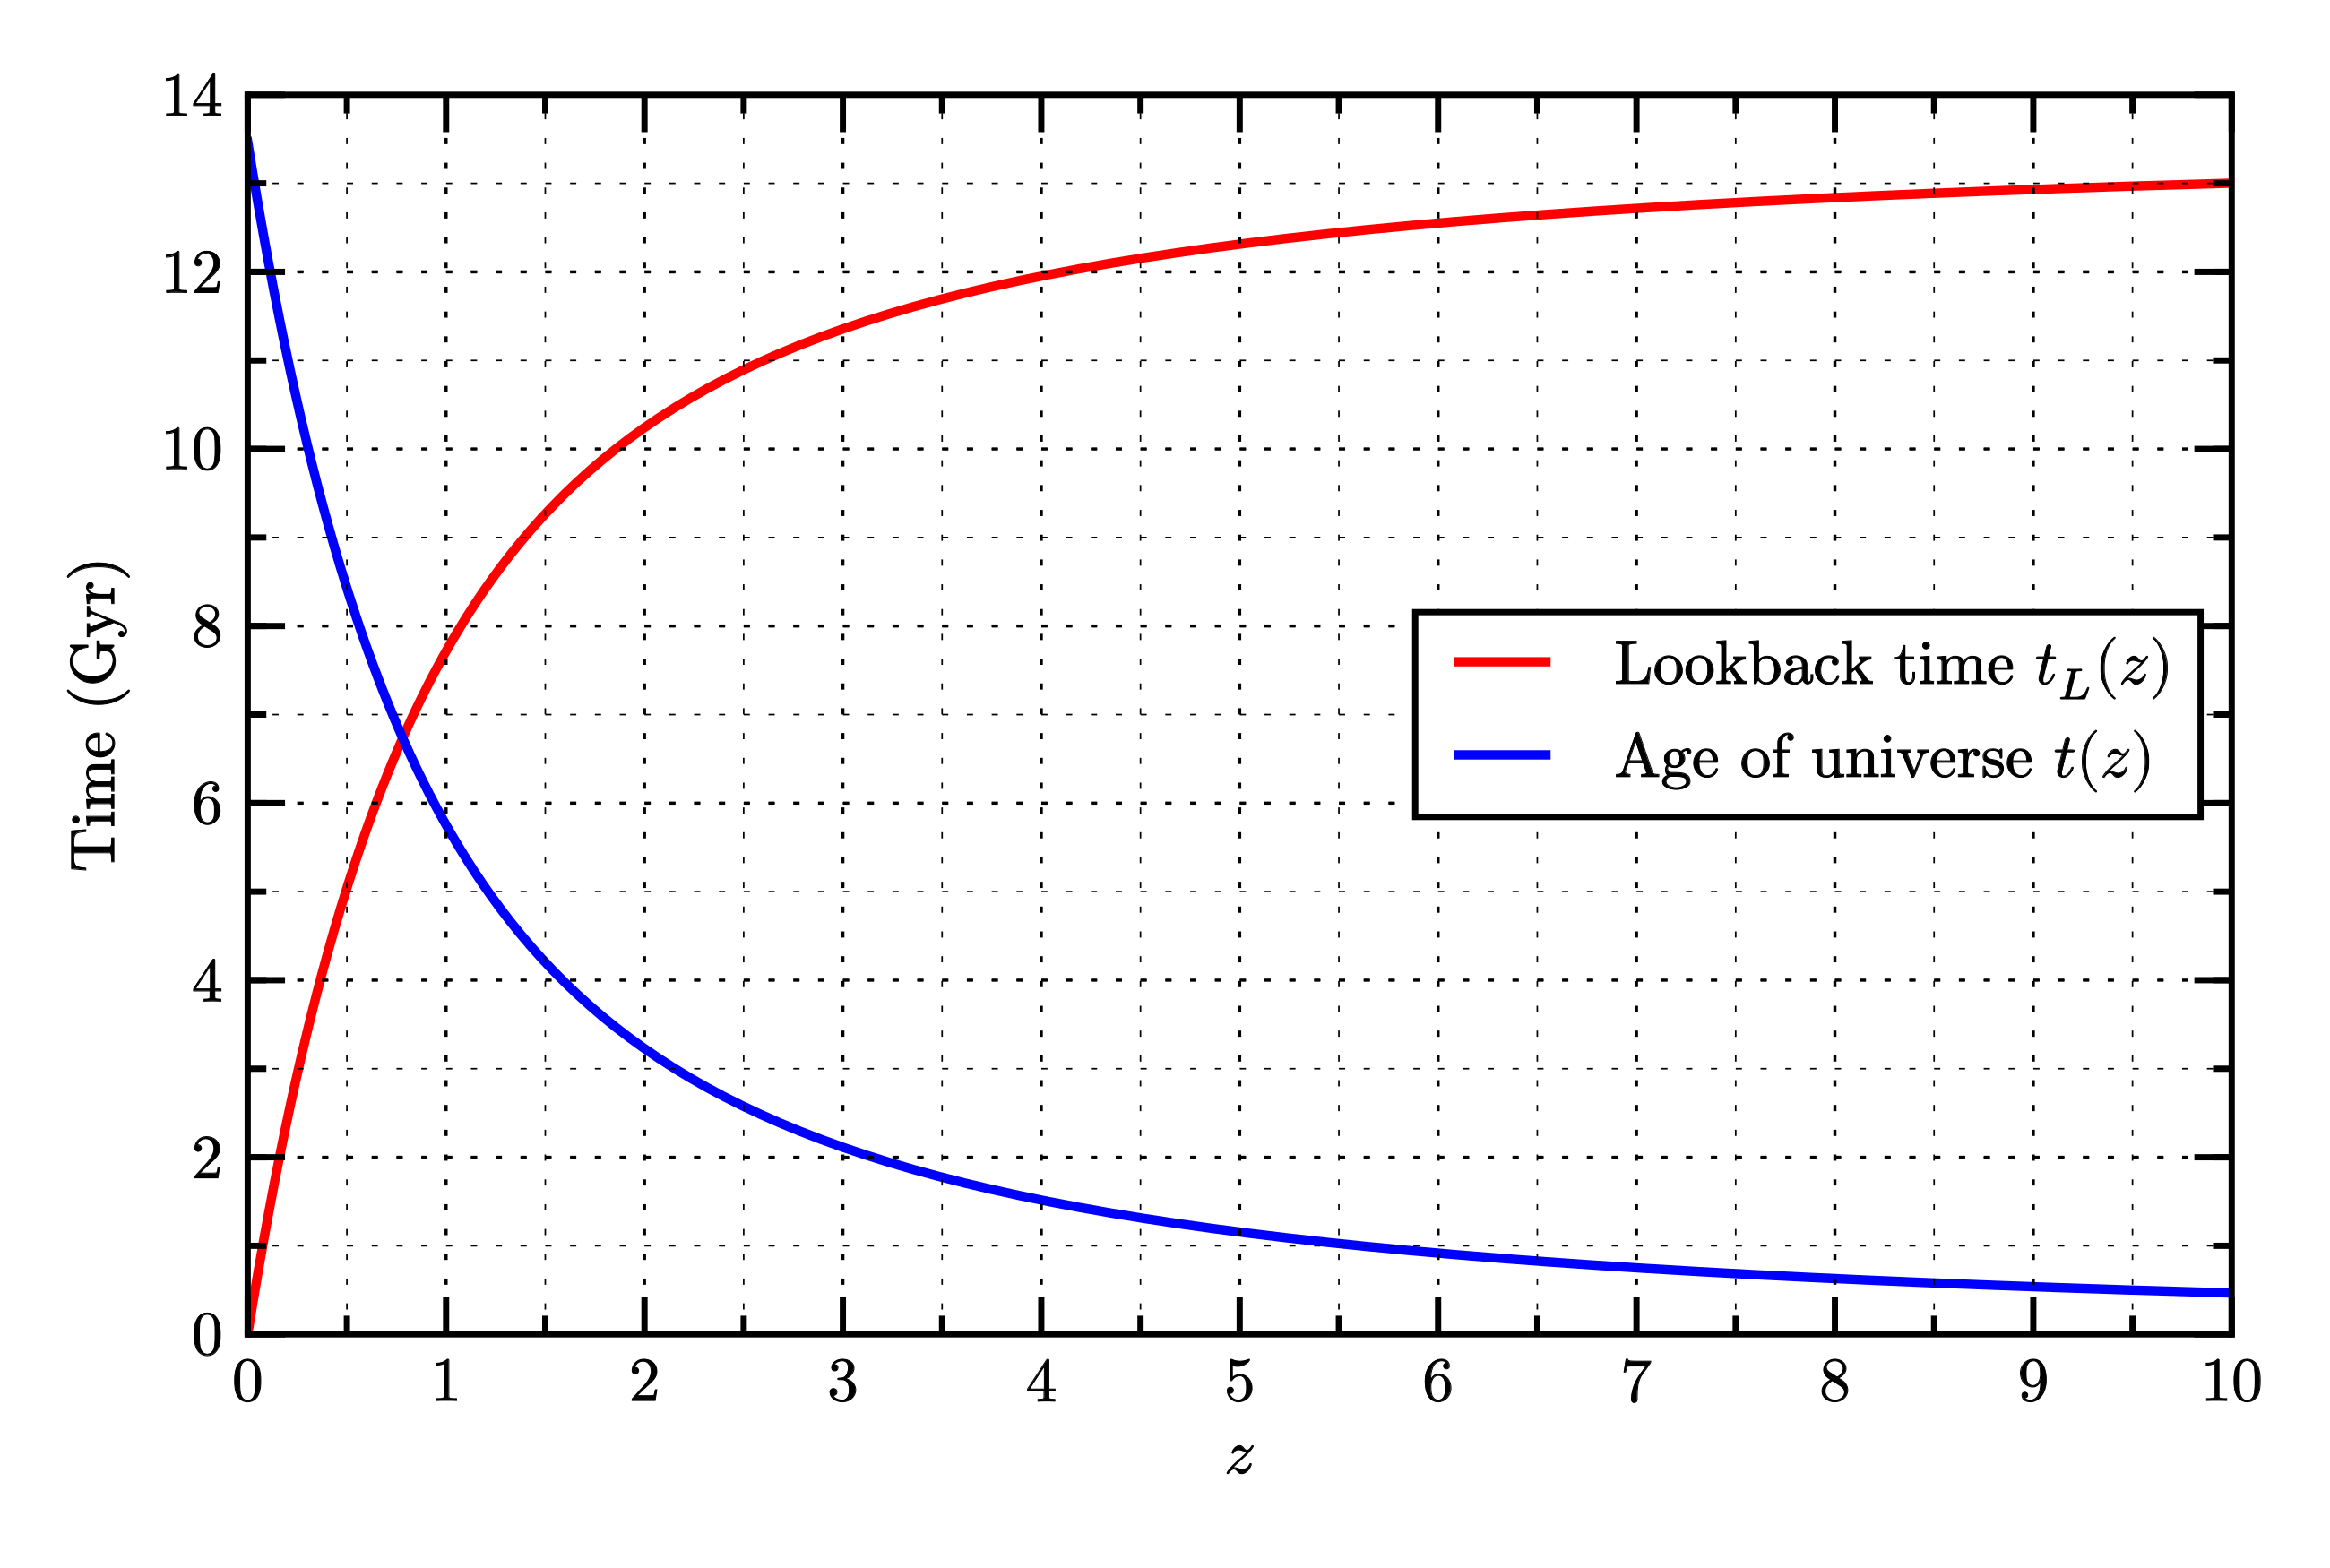
\includegraphics[width=0.95\textwidth]{Chapter1/Figs/lookback_time.png}
\caption[Relation between redshift and cosmic time]{The lookback time $t_L(z)$ and age of the universe $t(z)$ for an object observed at a redshift $z$, provided that its redshift is purely caused by cosmic expansion.} 
\label{fig:lookback_time}
\end{figure}

\noindent Here $\Omega_{R}$ is the present-day radiation density, $\Omega_{M}$ is the present-day total matter density, $\Omega_{\Lambda}$ is the present-day dark energy density, $\Omega_{k}=1-\Omega_{M}-\Omega_{\Lambda}$ is the curvature, and $H_{0}$ is the Hubble constant. Throughout this thesis, all calculations will assume\footnote{Even though the assumption of $\Omega_{R}=0$ is not strictly true, it is an excellent approximation in the matter-dominated era  with which this thesis is concerned, as measurements have shown that $\Omega_{R}\simeq 0.8 \times 10^{-4}$ \citep{2008ARA&A..46..385F}.} a cosmology of $\Omega_{M} = 0.3$, $\Omega_{\Lambda} = 0.70$, $\Omega_{R}=0$ and $H_{0} = \SI{70}{km.s^{-1}.Mpc^{-1}}$. In addition to the lookback time, the age of the universe $t$ when the light from an object at redshift $z$ was emitted can be found by changing the integration boundaries in Equation \ref{eqn:lookback_time} \citep{2008ARA&A..46..385F}: 

\begin{equation}
    t(z)= \frac{1}{H_{0}} \int_{z}^{\infty} \frac{ \diff z'}{(1+z')\sqrt{\Omega_{R}(1+z')^4+\Omega_{M}(1+z')^3+\Omega_{k}(1+z')^2+\Omega_{\Lambda}}}.
\end{equation}

To visualise the relation between cosmic time and redshift, the lookback time and age of the universe\footnote{A note from the author: it is interesting to note that the lookback time increases incrementally slowly with increasing redshift. The fact that the laws of physics cause this behaviour is highly serendipitous; it results in an extremely useful set of circumstances in which the history of the universe can be studied with increasing resolution further back in time. In this way, the redshifts of the very earliest galaxies provide a very precise handle to study the build-up of cosmic structure. --- A. L. S. } are both plotted as a function of redshift in Figure \ref{fig:lookback_time}.  \par




\paragraph{Measuring redshifts} 
The equations above illustrate why redshifts are so important to galaxy evolution studies: if it is possible to obtain redshift measurements, galaxies can be sorted by cosmic epoch, so that changing properties can be studied statistically as a function of time.  As implied by Equation \ref{eqn:redshift_definition}, redshifts can be found by comparing the wavelengths of certain features in an observed, i.e. redshifted, galaxy spectral energy distribution (SED) to their corresponding expected rest-frame wavelengths. The most precise way to do this involves spectroscopy, comparing the observed wavelengths of certain emission or absorption lines in a high-resolution spectrum to the wavelengths of these transitions as measured in a laboratory. Some astronomical surveys, such as the SDSS, incorporate this technique via a spectroscopic component  \citep{2012AJ....144..144B}. There have also been other projects that are exclusively spectroscopic, targeting galaxy candidates that have been selected from other imaging surveys (e.g. \citealt{2001MNRAS.328.1039C, 2005ApJ...620..595W,2005A&A...439..845L}).  \par

However, as will be discussed in more detail in Section \ref{section:photometric_redshifts}, obtaining spectra is time-consuming, and unfeasible for the huge catalogues produced by modern surveys. Nevertheless, even without a high-resolution spectrum that exhibits individual absorption or emission lines, it is often still possible to use colours from broadband filters to obtain an approximate redshift estimate. Examples of this method include photometric redshifts (see Section \ref{section:photometric_redshifts}) and colour cuts (exclusively for objects at $z\gtrsim3$; see Section \ref{subsubsection:lyman_break}). In this way, the redshifts of galaxies in the enormous surveys of the CCD era can be estimated using only the survey data itself.  \par


\subsubsection{Small area space-based surveys}\label{subsubsection:space_based_surveys}
With the power of distance measurements provided by redshift estimates, deep-field surveys can be an extremely powerful tool for galaxy evolution studies. The current section briefly reviews the developments in this fast-moving field of research.  \par


\afterpage{\newpage\begin{ThreePartTable}
\begin{TableNotes}
\item[] \hspace{-0.5em} \textbf{References}: \\
\item[i] \cite{1994AAS...185.5309G}
\item[ii] \cite{1996AJ....112.1335W}
\item[iii] \cite{2000AJ....120.2747C}
\item[iv] \cite{2004ApJ...600L..93G}
\item[v] \cite{2006AJ....132.1729B}
\item[vi] \cite{2005AJ....130....1T}
\item[vii] \cite{2013ApJS..209....6I}
\item[viii] \cite{2007ApJS..172....1S}
\item[ix] \cite{2007ApJ...660L...1D}
\item[x] \citealt{2011ApJS..197...35G, 2011ApJS..197...36K}

\vspace{0.5em}
\item[] \hspace{-0.5em} \textbf{Other comments}: \\
\item[a] The HXDF is assembled out of all Hubble data in the HUDF region. 

\item[] \hspace{-0.3em}\textit{Almost all fields in this table have been studied in several wavelengths since being released, but}
\item[] \hspace{-0.3em}\textit{the following projects contained further multiwavelength data as part of their core science goals:}
\item[b] Also contains X-ray, mid-IR, far-IR data; and ground-based optical, near-IR data. 
\item[c] Also contains X-ray, UV, mid-IR, far-IR data; and ground-based optical, near-IR, radio data.
\end{TableNotes}

\renewcommand\TPTminimum{\textwidth}
\setlength{\tabcolsep}{0.15em}
\centering
\footnotesize
\begin{longtable}{lcccccccccc}
\multicolumn{11}{c}{\normalsize \textsc{Small-scale space-based optical and near-infrared surveys}}\\
\toprule\toprule 
\endhead
\midrule\midrule
\multicolumn{11}{r}{\textit{continued}}
\endfoot
\insertTableNotes \\
\bottomrule\\
\caption[Small-scale space-based surveys]{Overview of major small-scale space-based surveys over optical (`visible'/`vis) and near-infrared (`NIR') wavelengths.}\label{table:space_small_survey}\\
\endlastfoot


Survey & Type & Epoch & Area &  \multicolumn{5}{c}{Bands, depth} & \si{\magab} & \textnumero{} galaxies \\
\midrule

GSS\tnote{i} & Visible & 1994 & \SI{127}{\sqarcmin} & \multicolumn{5}{c}{\begin{tabular}[t]{cc} $V_{606}$ & $I_{814}$ \\ 26.1 & 25.4 \end{tabular}} & $5\sigma$ & 11 000 \\ 
%Groth \cite{1994AAS...185.5309G}

HDF\tnote{ii} & Visible & 1995 & \SI{6.25}{\sqarcmin} & \multicolumn{5}{c}{\begin{tabular}[t]{cccc} $U_{300}$  & $B_{450}$ & $V_{606}$ & $I_{814}$ \\ 27.0 & 27.9 & 28.2 & 27.6  \end{tabular}} & $10\sigma$ & 3000 \\

HDF-S\tnote{iii} & Visible & 1998 & \SI{6.25}{\sqarcmin} & \multicolumn{5}{c}{\begin{tabular}[t]{cccc} $U_{300}$  & $B_{450}$ & $V_{606}$ & $I_{814}$ \\ 26.8 & 27.7 & 28.3 & 27.7  \end{tabular}} & $10\sigma$ & 2700 \\

GOODS\tnote{iv} & Visible\tnote{b} & 2002--2003 & \SI{320}{\sqarcmin} & \multicolumn{5}{c}{\begin{tabular}[t]{cccc} $B_{435}$ & $V_{606}$ & $i_{775}$ & $z_{850}$ \\ 27.8 & 27.8 & 27.1 & 26.6 \end{tabular}} & $10\sigma$ & 73 000  \\

HUDF\tnote{v} & Visible & 2003--2004 & \SI{11}{\sqarcmin} & \multicolumn{5}{c}{\begin{tabular}[t]{cccc} $B_{435}$ & $V_{606}$ & $i_{775}$ & $z_{850}$ \\ 29.1 & 29.5 & 29.4 & 28.7  \end{tabular}} & $10\sigma$ & 10 000 \\

NICMOS UDF\tnote{vi} & NIR & 2003 & \SI{5.8}{\sqarcmin} & \multicolumn{5}{c}{\begin{tabular}[t]{cc} $J_{110}$ & $H_{160}$  \\ 27.7 & 27.7  \end{tabular}} & $5\sigma$ & 1300 \\

%TALK ABOUT THIS IN THE TEXT

HXDF\tnote{vii,a} & Vis-NIR & 2002--2013 & \SI{11}{\sqarcmin} & \multicolumn{5}{c}{\begin{tabular}[t]{ccccc} $B_{435}$ & $V_{606}$ & $i_{775}$ & $I_{814}$ &  $z_{850}$ \\ 29.8 & 30.3 & 30.3 & 29.1 & 29.4 \\ \multicolumn{5}{c}{\begin{tabular}[t]{cccc} $Y_{105}$ & $J_{125}$ & $JH_{140}$ & $H_{160}$ \\ 30.1 & 29.8 & 29.8 & 29.8 \end{tabular}} \end{tabular}} & $5\sigma$ & 14 000\\


COSMOS\tnote{viii} &  {\begin{tabular}[t]{c} Visible\tnote{c} \\ \\ Visible\tnote{c} \\ \\ NIR\tnote{c} \\ \\ \end{tabular} } & 2003--2005 & {\begin{tabular}[t]{c} \SI{1.8}{\sqdeg} \\ \\  \SI{1.07}{\sqdeg} \\ \\ \SI{330}{\sqarcmin} \\ \\ \end{tabular}} &
\multicolumn{5}{c}{\begin{tabular}[t]{cc} $g_{475}$ & $I_{814}$ \\ 27.9 & 27.5 \\ $U_{300}$ & $B_{450}$ \\ 24.8 & 26.7 \\ \multicolumn{2}{c}{$H_{160}$} \\ \multicolumn{2}{c}{ 25.9 } \end{tabular}}   & $5\sigma$ &  {\begin{tabular}[t]{c} 1 700 000 \\ \\ \\ \\ 21 000  \\ \\ \end{tabular}} \\ 

AEGIS\tnote{ix} & {\begin{tabular}[t]{c} Visible\tnote{c} \\ \\ NIR\tnote{c} \\ \\ \end{tabular} } & 2004--2005 &  {\begin{tabular}[t]{c} \SI{700}{\sqarcmin} \\ \\ \SI{46}{\sqarcmin} \\ \\ \end{tabular}} & \multicolumn{5}{c}{\begin{tabular}[t]{cc} $V_{606}$ & $I_{814}$ \\ 28.1 & 27.5 \\ $J_{110}$ & $H_{160}$ \\ 25.7 & 25.5 \end{tabular}} & {\begin{tabular}[t]{c} $5\sigma$ \\ \\ $10\sigma$ \\ \\ \end{tabular} } & {\begin{tabular}[t]{c} 80 000 \\ \\ 4000 \end{tabular}}  \\ 

CANDELS\tnote{x} & Vis-NIR & 2010--2013 &  \multicolumn{5}{c}{} & & $5\sigma$  & 250 000 \\

\multicolumn{1}{l}{\textit{Wide}} & & & \SI{770}{\sqarcmin} & \multicolumn{5}{c}{\begin{tabular}[t]{ccc} \multicolumn{3}{c}{\begin{tabular}[t]{cc}  $V_{606}$ & $I_{814}$ \\ 27.6 & 27.5 \end{tabular} } \\ \multicolumn{3}{c}{ \begin{tabular}[t]{ccc}  $Y_{105}$ & $J_{125}$ & $H_{160}$  \\ 26.6 & 26.4 & 26.5 \end{tabular} } \\\end{tabular}} &  & \\

\multicolumn{1}{l}{\textit{Deep}} & & & \SI{120}{\sqarcmin} & \multicolumn{5}{c}{\begin{tabular}[t]{ccccc}  $B_{435}$ & $V_{606}$ & $i_{775}$ & $I_{814}$ & $z_{850}$ \\ 27.8 & 28.2 & 27.5 & 28.4 & 27.3 \\ 
\multicolumn{5}{c}{ \begin{tabular}[t]{ccc}  $Y_{105}$ & $J_{125}$ & $H_{160}$  \\ 27.3 & 27.4 & 27.2 \end{tabular} } \\  \end{tabular}} &  & \\

\end{longtable}
\end{ThreePartTable}
}



The prototype for the modern concept of extremely deep fields is the Hubble Deep Field (HDF; \citealt{1996AJ....112.1335W}), imaged by the \textit{HST}. The space-borne nature of this instrument makes it especially well suited to extremely deep imaging. Because it avoids blurring by the Earth's atmosphere, images can be more detailed and deeper, as light is spread out over fewer pixels. The HDF contains 3000 galaxies with magnitudes of up to $V \sim \SI{30}{\mag}$ for the faintest sources, and several objects with redshifts of $z>5$. The Hubble Ultra Deep Field (HUDF; \citealt{2006AJ....132.1729B}) and the Hubble Extreme Deep Field (HXDF; \citealt{2013ApJS..209....6I}) imaged the same region of the sky as the original HDF, over larger areas and with newer cameras. These surveys achieved even higher depths and pushed the discovery of high-redshift galaxies to $z\sim7$ and $z\sim12$ respectively, reaching the very limit of what is possible with current technology. Table \ref{table:space_small_survey} presents a summary of some core properties of the Hubble Deep Field surveys. \par 



After the success of the Hubble Deep Fields, further deep \textit{HST} surveys followed.   Progress was mainly made in the direction of larger areas and more wavelength coverage. This helped to build up a more comprehensive picture of galaxy evolution, as the larger size of the observed fields allowed the assembly of larger, statistically significant samples to study changes in galaxy populations. Table \ref{table:space_small_survey} summarises several noteworthy examples of these surveys. Each one specialised in a specific redshift regime, but together they cover cosmic time between roughly $0.5\lesssim z \lesssim 8$. Examples of galaxy properties that have been studied with these datasets include mass assembly, the coupled evolution of galaxies, active galactic nuclei (AGN), and large-scale structure. The bigger sample sizes also facilitated applications in cosmology, such as studies of dark matter through gravitational lensing. \par  


\subsubsection{Intermediate-area ground-based surveys}\label{subsubsection:ground_based_surveys}
A major downside to space-based surveys is that the main optical and near-IR instrument is the \textit{HST}, which has a very restricted amount of available observing time and a limited field of view compared to ground-based telescopes. On top of that, ground-based telescopes are more cost-effective for larger surveys, especially for areas over $\sim \SI{1}{\sqdeg}$. To capitalise on these advantages, astronomers have started to conduct intermediate-area deep surveys from the ground, often utilising the sophisticated terrestrial instruments developed during the CCD revolution (described in Section \ref{subsection:technological_advancements}).  Such intermediate surveys cover several square degrees, to much higher depths than the large-scale wide-area projects from Section \ref{subsection:technological_advancements}. In this way, they can cover much more area than space-based ones, although they are generally not quite as deep and have much lower image resolution due to atmospheric blurring. \par 


\afterpage{\newpage\begin{ThreePartTable}
\begin{TableNotes}
\item[] \hspace{-0.5em} \textbf{References}: \\
\item[i] \cite{1999ASPC..191..111J}
\item[ii] \cite{2002SPIE.4836...73W}
\item[iii] \cite{2004PASJ...56.1011K}
\item[iv] \cite{2008ApJS..176....1F}
\item[v] \cite{2012AJ....143...38G}
\item[vi] \cite{2007MNRAS.379.1599L}
\item[vii] \cite{2013MNRAS.428.1281J}
\item[viii] \cite{2012A&A...544A.156M}
\item[ix] \cite{2012ApJ...753..152B,2016MNRAS.460.1270D}


\vspace{0.5em}
\item[] \hspace{-0.5em} \textbf{Other comments}: \\
\item[a] Because galaxy counts were not provided, these are total source counts. \\
\item[b] These are the expected final depths for point sources from the full five years of observations. They differ from the depths for the DES data presented later in this thesis (Table \ref{table:actual_des} and Figure \ref{fig:area_depth}), which are for a \SI{1.95}{\arcsec} aperture using only the first year of observations. 
\end{TableNotes}

\renewcommand\TPTminimum{\textwidth}
\setlength{\tabcolsep}{0.15em}
\centering
\footnotesize
\begin{longtable}{lcccccccccc}
\multicolumn{11}{c}{\normalsize \textsc{Intermediate-scale ground-based optical and near-infrared surveys}}\\
\toprule\toprule 
\endhead
\bottomrule
\multicolumn{11}{r}{\textit{continued}}
\endfoot
\insertTableNotes \\
\bottomrule\\
\caption[Intermediate-scale ground-based surveys]{Overview of major intermediate-scale ground-based surveys over optical (`visible'/'vis') and near-infrared (`NIR') wavelengths.}\label{table:ground_small_survey}\\ 
\endlastfoot

Survey & Type & Epoch & Area &  \multicolumn{5}{c}{Bands, depth} & \si{\magab} & \textnumero{} galaxies \\
\midrule

NDWFS\tnote{i} & Vis-NIR & 1997--1999 & \SI{9}{\sqdeg} & \multicolumn{5}{c}{\begin{tabular}[t]{cccc} $B_{w}$ & $R$ & $I$ & $K$ \\ 27.2 & 26.3 & 25.9 & 21.0 \end{tabular}}  & $5\sigma$ & 3 200 000\tnote{a} \\

DLS\tnote{ii} & Visible & 2001--2006 & \SI{20}{\sqdeg} & \multicolumn{5}{c}{\begin{tabular}[t]{cccc} $B$ & $V$ & $R$ & $z'$ \\ 26.6 & 26.5 & 26.9 & 24.8  \end{tabular}} & $5\sigma$ & 5 000 000 \\
%\cite{2002SPIE.4836...73W} 

%\cite{1999ASPC..191..111J}
SDF\tnote{iii} & Visible & 2002--2004 & \SI{920}{\sqarcmin} & \multicolumn{5}{c}{\begin{tabular}[t]{ccccc} $B$ & $V$ & $R$ & $i'$ & $z'$ \\ 28.5 & 27.7 & 27.8 & 27.4 & 26.6  \end{tabular}} & $3\sigma$ & 210 000 \\
%\cite{2004PASJ...56.1011K}

SDXF\tnote{iv} & Visible &  2002--2005 & \SI{1.2}{\sqdeg} & \multicolumn{5}{c}{\begin{tabular}[t]{ccccc} $B$ & $V$ & $R_{c}$ & $i'$ & $z'$ \\ 28.4 & 27.8 & 27.7 & 27.7 & 26.6  \end{tabular}} & $3\sigma$ & 900 000\tnote{a} \\

CFHTLS-D\tnote{v} & Visible & 2003--2009 & \SI{4}{\sqdeg} & \multicolumn{5}{c}{\begin{tabular}[t]{ccccc} $u*$ & $g'$ & $r'$ & $i'$ & $z'$ \\ 27.5 & 27.9 & 27.9 & 27.7 & 26.5 \end{tabular}} & $5\sigma$ & > 300 000 \\

UKIDSS-UDS\tnote{vi} & NIR & 2005--2012 & \SI{0.77}{\sqdeg} & \multicolumn{5}{c}{\begin{tabular}[t]{ccc} $J$ & $H$ &  $K$ \\ 26.3 & 26.0 & 25.6  \end{tabular}} & $5\sigma$ & 250 000 \\

UKIDSS-DXS\tnote{vi} & NIR & 2005--2012 & {\begin{tabular}[t]{c}  \SI{35}{\sqdeg} \\ \\ \SI{5}{\sqdeg} \\ \end{tabular}} & \multicolumn{5}{c}{\begin{tabular}[t]{cc} $J$  &  $K$ \\ 23.4 & 22.9 \\ \multicolumn{2}{c}{$H$} \\ \multicolumn{2}{c}{23.4} \end{tabular}} & $5\sigma$ & 3 000 000\tnote{a} \\
%\cite{2007MNRAS.379.1599L}


VIDEO\tnote{vii} & NIR & 2009--2018 & \SI{12}{\sqdeg} & \multicolumn{5}{c}{\begin{tabular}[t]{ccccc} $Z$ & $Y$ & $J$ & $H$ & $K_{s}$ \\ 25.7 & 24.5 & 24.4 & 24.1 & 23.8 \end{tabular}} & $5\sigma$ & 1 700 000\tnote{a} \\
%\cite{2013MNRAS.428.1281J}

UltraVISTA\tnote{viii} & NIR & 2009--2018 & \multicolumn{5}{c}{}  & & $5\sigma$ & 200 000\tnote{a} \\

\multicolumn{1}{l}{\textit{Deep}} & & & \SI{1.5}{\sqdeg} & \multicolumn{5}{c}{\begin{tabular}[t]{cccc} $Y$ & $J$ & $H$ & $K_{s}$ \\ 24.8 & 24.5 & 24.1 & 23.8 \\  \end{tabular}}  &  & \\

\multicolumn{1}{l}{\textit{Ultra-Deep}} & & & \SI{0.73}{\sqdeg} & \multicolumn{5}{c}{\begin{tabular}[t]{cccc} $Y$ & $J$ & $H$ & $K_{s}$ \\ 25.7 & 25.4 & 25.1 & 24.1 \\  \end{tabular}}  &  & \\

DES Deep\tnote{ix}\tnote{b} & Visible & 2013--2019 & & \multicolumn{5}{c}{} & $5\sigma$ & 2 000 000 \\

\multicolumn{1}{l}{\textit{Shallow}} & & & \SI{24}{\sqdeg} & \multicolumn{5}{c}{\begin{tabular}[t]{cccc} $g$ & $r$ & $i$ & $z$ \\  27.7  & 26.5 & 26.8 & 26.6  \\  \end{tabular}}  &  & \\

\multicolumn{1}{l}{\textit{Deep}} & & & \SI{6}{\sqdeg} & \multicolumn{5}{c}{\begin{tabular}[t]{cccc} $g$ & $r$ & $i$ & $z$ \\  28.0 & 28.2 & 27.9 & 27.7  \\  \end{tabular}}  &  & \\

\end{longtable}
\end{ThreePartTable}
}



Their position between the shallow wide-area ground-based surveys and the ultra-deep narrow space-based surveys makes intermediate-scale surveys ideal for intermediate applications. As will be illustrated in more detail below, they are often used to collect larger samples than possible with space-based surveys, in order to improve sample statistics. Furthermore, they are more likely to contain rare objects that require a larger search area. Intermediate-scale surveys can also unveil cosmological structures larger than the few Mpc scales probed by space-based surveys, and can reduce biases introduced by cosmic variance. On top of that, they offer a significant increase in lookback time over wide-area surveys. Their major downside is that they are not able to reach quite as high redshifts as the space-based datasets, so they generally cannot be used to find the  utmost distant sources. \par

%at the same time, they offer...

%For many intermediate-scale surveys, a larger observational footprint has offered significant scientific advantages. 

Table \ref{table:ground_small_survey} lists several important examples of intermediate-scale surveys. For many of these, a larger observational footprint has offered significant scientific advantages. A common research goal has been to collect large samples for improving population statistics. For instance, the Subaru Deep Field (SDF) survey revealed statistically significant samples of Lyman-break galaxies at $z \approx \numrange{4}{5}$ and Lyman-$\alpha$ emitters at $z \approx \numrange{5}{6} $. Similarly, the UKIDSS Deep Extragalactic Survey (UKIDSS-DXS) aimed to facilitate a statistical study of galaxy properties at $z\sim 1$, to compare with the $z\sim 0$ picture from local surveys such as SDSS. Furthermore, UltraVISTA has enabled a representative study of the peak of star formation at $2<z<3$, and the VISTA Deep Extragalactic Observations (VIDEO) survey has been targeted at providing a comprehensive view of the evolution of galaxies with their environment out to $z\approx4$. A second commonly occurring goal of the surveys in question has often involved finding uncommon objects. Rare object searches have included AGN searches in the VIDEO survey, the deep component of the Canada-France-Hawaii Telescope Legacy Survey (CFHTLS-D), and the NOAO Deep Wide Field Survey (NDWFS). Additionally, the most luminous galaxies can be studied at $3<z<5$ in the CFHTLS-D, at $z>4$ in the NDWFS, and out to $z\approx7$ in UltraVISTA and the UKIDSS Ultra-Deep Survey (UKIDSS-UDS). Ultravista was also designed to uncover galaxies at the highest redshifts ($ z \simeq 6.5--9$). A third aim of some ground-based surveys, such as the Dark Energy Survey Deep Fields and CFHTLS-D, has been to look for Type Ia supernovae to constrain dark energy. Lastly, the fourth major application of intermediate-scale surveys concerns studies of large-scale structure for the purpose of constraining cosmological parameters. Examples include the Subaru Deep XMM-Newton Survey (SDXF), NDWFS, and the Deep Lens Survey (DLS), the latter of which specifically focused on weak gravitational lensing. \par 



\subsection{Multiwavelength datasets}\label{subsection:multiwavelength}
Many of the astronomical surveys that have been discussed often cover a particular wavelength regime, generally  optical or near-infrared. Their scientific successes show that each such dataset can be incredibly powerful on its own. However, in many cases, combining observations from surveys over multiple wavebands can open up further opportunities for interesting discoveries. \par 
%SMOOTHE IT UP

Historically, the combination of surveys over a wide range of the electromagnetic spectrum has been very fruitful. Perhaps the oldest and simplest application of such a multiwavelength approach is the use of optical data for the identification of sources that were discovered in other frequencies. For instance, in the early ages of infrared and radio astronomy, the physicists that pioneered these fields often turned to the optical POSS-I survey (see Section \ref{subsection:history}) for this purpose. Other historical examples where combining datasets from different wavelengths has revealed results that could not be recognised in a single dataset alone include the discovery of quasars (QSOs) and ultraluminous starbursts, and the interpretation of $\gamma$-ray bursts (see \citealt{2013pss2.book..223D}). \par


To capitalise on the opportunities offered by multiwavelength astronomy, contemporary observations are often coordinated between instruments specialising in different wavelength regimes. In particular, several of the small and intermediate area surveys from Tables \ref{table:space_small_survey} and \ref{table:ground_small_survey} have been designed as part of a collaboration of different instruments, and some others have later been followed up at other wavelengths. These developments are moving astronomy into a regime where the energetic output of a source can be traced throughout large parts of the electromagnetic spectrum. The study of galaxy evolution is one research area that particularly benefits from the great scientific power of panchromatic datasets, and the following two sections will present two examples. \par 

\subsubsection{Uncovering galaxy properties with multiwavelength data}
The first asset of a multiwavelength approach is that different frequencies trace different galaxy properties. To name a few examples, optical imaging unveils their positions and morphologies, as well as possible environmental disruptions such as mergers with neighbouring objects \citep{2010MNRAS.401.1043D,2017MNRAS.464.4176W}. Near-infrared data can be valuable as well, for instance for measuring stellar masses \citep{2003ApJS..149..289B}. Furthermore, X-ray, mid-infrared, and radio observations can detect AGN, including those obscured by dust \citep{2018ARA&A..56..625H}. X-ray data can also be used to find hot intergalactic gas around galaxy mergers and clusters \citep{2006ApJ...643..692C,2018MNRAS.475.2067B}. Finally, information from the ultraviolet, mid-IR, and radio wavebands can track the rate of active star formation \citep{2017ApJ...847..136B}. \par 

The wavelength regimes listed above generally apply to the rest-frame emission. When objects are redshifted, the wavebands required to trace certain galaxy properties will become redder. For instance, as will be discussed in detail in Section \ref{subsubsection:lyman_break}, galaxies generally show a sharp break at (rest-frame) wavelengths of $\lambda=\SIrange{912}{1216}{\angstrom}$, emitting very little flux below this cutoff. At $z>6$, this cutoff is redshifted to $\lambda>\SI{8500}{\angstrom}$, so sources at these distances will emit almost all their flux in the observed near-infrared and beyond. Therefore, imaging at $\lambda> \SI{8500}{\angstrom}$ will be needed to observe them at all. Furthermore, properties which are locally measured at UV wavelengths, such as the star formation rate, are traced by observed-frame near-IR imaging at these high redshifts. \par

 
\subsubsection{The benefits of multiwavelength data for estimating redshifts}\label{subsubsection:multiwavelength_redshifts}

The second core strength of multiwavelength datasets involves improved redshift estimates from broadband colours. Such measurements generally rely on several strong spectral features in galaxy rest-frame UV and optical emission (most importantly the Lyman limit at $\lambda = \SI{912}{\angstrom} $, the $\lambda=\SI{1216}{\angstrom}$ break, the Balmer break at $\lambda=\SI{3646}{\angstrom}$, and the $\lambda = \SI{4000}{\angstrom}$ break). However, with increasing redshift, these features will trivially shift towards longer wavelengths, so that redder imaging becomes more and more important. For instance, at $z>1.5$ the \SI{4000}{\angstrom} break has redshifted out of the optical and into the near-IR. Secondly, as mentioned earlier, beyond $z>6$ the observed emission from galaxies --- and hence all their important spectral features --- lies almost entirely in the near-IR and beyond. Therefore, near-infrared imaging is almost always necessary to determine redshifts for $z>6$ galaxies  \citep{2009MNRAS.395.2196M,2014MNRAS.440.2810B}. This point will be revisited later in Section \ref{subsubsection:lyman_break_galaxy_history}. \par




A particularly common method for estimating redshifts in modern astronomy is the so-called photometric redshift technique. An in-depth discussion of this method will follow shortly in Section \ref{section:photometric_redshifts}, where it will be shown that this is a highly effective technique for obtaining redshift estimates from broadband fluxes in large surveys. The photometric redshift approach essentially computes the redshift of a given object by using its broadband colours as a very low resolution spectrum. Simple statistics prima facie dictate that adding data in more filters will improve the resulting redshift estimates, simply by increasing the amount of available information. The most striking example of this is perhaps the photometric redshift catalogue for the COSMOS field \citep{2009ApJ...690.1236I}. With 30 broadband colours covering the UV, optical, near-IR, and mid-IR, the accuracy of this panchromatic dataset approaches that of spectroscopic redshifts (when compared with spectroscopic redshifts $\Delta z= z_{\mathrm{spec}} - z_{\mathrm{phot}}$, the dispersion is $\sigma_{\Delta z/ (1+z_{\mathrm{spec}})} =0.007$ for sources brighter than $i^{+}_{\mathrm{AB}}<22.5$).  Furthermore, several simulations \citep{2008MNRAS.386.1219B,2008MNRAS.387..969A} and observational studies \citep{2009ApJ...690.1236I,2013MNRAS.428.1281J,2015MNRAS.446.2523B} have indicated that photometric redshift estimates benefit from including infrared data in particular.  Altogether, it is therefore clear that combining surveys from multiple wavebands is beneficial to galaxy evolution studies (as well as many areas of astronomy in general). \par 


\subsection{Conclusion on surveys}\label{subsection:conclusion_surveys_intro}
We have now reached the end of our birds-eye-view journey through survey astronomy, which forms the first part of the introduction to this thesis. Along the way, we have seen how advances in technology and instrumentation have given rise to a situation where celestial sources can now be discovered electronically millions or billions at a time. Thanks to this data-driven revolution, the last 30 years can undoubtedly be characterised as the CCD era of astronomy. This period has witnessed large-scale wide surveys imaging substantial parts of the sky, as well as smaller deeper surveys unveiling increasingly distant cosmic structures. We have also seen how combining observations over multiple wavelength regimes can often increase the scientific potential of surveys even further. The enormous datasets resulting from all of these developments have led to many new discoveries across several branches of astronomy, and there are doubtlessly many more to come. \par 

But the explosion of data also comes with certain obstacles. Some of these, such as the infrastructure needed to process the gigantic data streams, lie within the realm of technology and computer science. Other challenges are computational and astrophysical in nature, and concern the extraction of physically meaningful quantities from survey data.It is aspects from the latter category that the current text will address. \par

%It is aspects from the latter category that the current work {\color{red}has taken up}.

%

%As part of this, the first part of this thesis will focus on the task of combining

%As part of this, the first part of this thesis will address the task of combining optical and near-infrared data from two deep intermediate-area ground-based surveys to create a single, more powerful multiwavelength catalogue.

As part of this, the first part of this thesis will focus on the task of combining optical and near-infrared data from two deep intermediate-area ground-based surveys to create a single, more powerful multiwavelength catalogue. This new merged data product can harness the potential of panchromatic datasets, creating a useful resource for the rest of this thesis as well as for the scientific community. The next part of the thesis will then describe the process of acquiring distance estimates for all objects in the catalogue. This is achieved through photometric redshifts, and this computational method forms the topic of the next part of this introduction.  \par




\section{Photometric redshifts}\label{section:photometric_redshifts}
Many branches of research in modern extragalactic astronomy rely crucially on distance measurements. As mentioned previously in Section \ref{subsubsection:redshift_interlude}, spectroscopic redshifts generally offer the most accurate way of doing this. However, for a multitude of reasons that will be discussed imminently, it is not always feasible to measure redshifts spectroscopically. To circumvent this problem, photometric redshifts (photo-zs) can be measured from broadband magnitudes only. The idea is simple: multiband photometry is essentially a very low resolution spectrum, and can therefore be used to estimate redshifts \citep{1998astro.ph..9347Y}. Primarily, this tactic relies on broad spectral features that exist in the emission of most galaxies (predominantly the Lyman break at $\lambda = \SIrange{912}{1216}{\angstrom}$ and the Balmer/\SI{4000}{\angstrom} break). The photometric redshift approach has two major strengths: 

%GENERALLY=ON THE WHOLE

\begin{enumerate}
    \item Photometric redshifts can be computed for a far larger number of objects than is feasible with spectroscopy. The catalogues of modern surveys in the CCD era can contain millions or billions of galaxies. Despite the efficiency of modern multi-object spectrographs, it is only possible to measure meaningful spectra for a few percent of these sources, as spectroscopy is relatively time-consuming \citep{2005A&A...439..845L,2019NatAs...3..212S}. On the other hand, broadband magnitudes can be extracted directly from the imaging, which is obtained for all objects in the field of view simultaneously. The remaining problem of estimating the photo-zs is computational in nature, but the time required for this is minimal compared to the duration of spectroscopy. The latter issue is especially pressing for high-redshift research, as even the most luminous galaxies at redshifts $z \sim 6$ are so faint that they require integration times of several hours (e.g. \citealt{2013AJ....145....4W}). This makes spectroscopy an unfeasible method to search for such distant sources, which are extremely rare compared to the abundance of low-redshift galaxies. 
    
    \item The photometric redshift method can be used on sources for which conventional spectroscopy is not possible. As it relies only on broadband magnitudes, the technique can be applied to all galaxies in a given source catalogue, including objects with very low apparent brightness all the way out to a survey's imaging limits \citep{1998astro.ph..9347Y,2019NatAs...3..212S}. These faint sources that lie outside the current realm of spectroscopy include very small galaxies or galaxies at extremely high redshifts. 
\end{enumerate}

\noindent These two advantages have made the use of photometric redshifts ubiquitous for large datasets, and the method has become an integral part of data processing in galaxy surveys \citep{2013ApJ...775...93D}. The following sections will give a historical overview of the development of photo-zs and discuss specific techniques available in the literature. \par

\subsection{Historical overview}\label{subsection:photoz_history}
\cite{1962IAUS...15..390B} was the first ever author to use broadband photometry for estimating galaxy redshifts. He computed photo-zs by comparing magnitudes in nine photometric filters to spectra from galaxies in the Virgo cluster.  After that, the next occurrence of the photometric method was not until the 1980s, when it was once again employed by several authors. Butchins (\citeyear{1981A&A....97..407B}, \citeyear{1983MNRAS.203.1239B}), \cite{1982ApJ...257L..57P}, and \cite{1985AJ.....90..418K} all estimated photometric redshifts by comparing colours from photographic plates to those derived from template galaxy SEDs. Midway through the decade, \cite{1986ApJ...303..154L} first pioneered the use of CCD photometry. After these initial developments, the photometric redshift method remained relatively unused for the next 10 years, but from the middle of the 1990s it experienced a resurgence. The main reasons for this revival were twofold:

 


\begin{itemize}
    \item As the data revolution of the CCD era took off in the 1990s, broadband photometry could suddenly be obtained efficiently for huge samples of galaxies. The object counts of the resulting source catalogues were far too high to perform spectroscopy for every object, so it became necessary to use a more efficient method for distance measurements. In order to meet this need, many authors turned to photometric redshifts. 
    
    \item The publication of the HDF (see Section \ref{subsubsection:space_based_surveys}) provided a dataset containing galaxies with magnitudes out to $V \sim \SI{30}{\magab}$. Such sources are far too faint for conventional spectroscopy, necessitating the use of photometric redshifts. 
\end{itemize}


    
With these factors as impetuses for further development and refinement of the photo-z approach, many papers followed soon after (e.g. \citealt{1995AJ....110.2655C,1997ApJ...482L..21B,1998AJ....116.2081W,1996Natur.381..759L,1996ApJ...468L..77G,1996A&A...314...73P}). As the number of existing surveys and their source counts continued to rise while the CCD era advanced, the use of photometric redshifts grew even more widespread. More codes became available in the literature, and the available methods became more sophisticated. These developments will shortly be detailed further in Section \ref{subsection:methods}, which will describe in detail the variety of codes that have been created over the last three decades.  As the use of photometric redshifts became standard practice, many scientists started to make their photo-z methods publicly available. The first such public code was \texttt{HyperZ} \citep{2000A&A...363..476B}. Many others soon followed, including \texttt{BPZ} \citep{2000ApJ...536..571B},  \texttt{ANNz} \citep{2004PASP..116..345C},  \texttt{ZEBRA} \citep{2006MNRAS.372..565F},  \texttt{LePHARE} \citep{2006A&A...457..841I,2011ascl.soft08009A}, \texttt{EAZY} \citep{2008ApJ...686.1503B}, \texttt{ArborZ} \citep{2010ApJ...715..823G}, \texttt{TPZ} \citep{2013MNRAS.432.1483C,2010ApJ...712..511C} and \texttt{GPz} \citep{2016MNRAS.462..726A}. \par 


\subsection{Methods}\label{subsection:methods}
\cite{2011Ap&SS.331....1W} and \cite{1998astro.ph..9347Y} identify two main photometric redshift strategies commonly used in the literature. \textit{Empirical methods} employ a subset of objects with measured spectroscopic redshifts as a training set. This subset is used to determine an empirical relation between (spectroscopic) redshift and galaxy properties such as colour and magnitude. Photometric redshifts are then inferred by applying this relation to the entire dataset. \textit{Template methods} use pre-existing galaxy spectral energy distributions --- also known as templates --- from models or libraries of observed spectra. These SEDs can be stretched to any redshift, and predicted magnitudes can be computed by convolving the shifted SEDs with the transmission curves used in the relevant survey. For each object, all the predicted magnitudes are then compared to the observed photometry to find the best-fitting redshift and template combination. The following two sections will describe both empirical and template methods in more detail. \par 


\subsubsection{Empirical methods}\label{subsubsection:empirical_methods}
As mentioned above, empirical methods rely on a training sample to  calibrate a relation $z=z(C,m_{0})$ between redshift $z$ and observed colours $C$ or magnitudes $m_{0}$ \citep{2000ApJ...536..571B}. The phrase empirical refers to the fact that this relation is derived empirically from data in the training sample  only. \par 

The first empirical methods were developed when photometric redshifts rose to prominence in the mid-1990s. These early approaches were simple yet powerful. Even fitting functions $z=z(C,m_{0})$ where $z$ is a linear function or simple polynomial proved effective at estimating redshifts when appropriately tuned \citep{1995AJ....110.2655C}. For example, \cite{1998AJ....116.2081W} computed photo-zs via a linear relationship between redshift and three photometric colours ($U-B$, $B-V$, and $V-I$). The simple polynomial approach was applied successfully by e.g. \cite{1995AJ....110.2655C}, who fitted a second order polynomial to $U$, $B_{J}$, $R_{F}$ and $I_{N}$ magnitudes, and by \cite{1997ApJ...482L..21B}, who employed an iterative process with several quadratic functions of $U$, $B$, $R$, and $I$ magnitudes. \par

Early such forms of the empirical method proved superior to template methods \citep{2011Ap&SS.331....1W} for a number of reasons. Firstly, because the training set consists of real galaxies, there can be no issues with inaccurate templates. On top of that, the empirical relation is calibrated using magnitude measurements from survey data, so it inherently accounts for the effects of filter bandpasses and flux calibrations. Empirical methods can also easily provide realistic estimates of redshift uncertainties \citep{2011Ap&SS.331....1W}, and they generally outperform template methods in terms of speed as well \citep{2004A&A...423..761V,2019NatAs...3..212S}.  \par

A disadvantage of the empirical approach is that the derived relation $z=z(C,m_{0})$ is only valid for the full survey if the training set is representative, that is, if the training set has similar observables $C$ and $m_{0}$ to the full survey. This can be an issue when calculating photo-zs for objects much fainter than the training set (such as at high redshifts), because the relation has to be extrapolated in those cases.  Another problem is that galaxies at redshifts beyond those in the training sample may have different intrinsic SEDs. A further,  related drawback is that the sample also needs to be large enough to cover all colours, magnitudes, galaxy types, and redshifts to a statistically significant degree, so that the inferred empirical relation is statistically sound. \par

Empirical photo-z codes have become more advanced since the early methods described before, making use of sophisticated computational techniques which have developed alongside the field of machine learning. The core idea of these approaches is still the same as for the simple early methods: through machine learning, a training set is used to build up a relationship  between survey observables and redshifts. Examples of specific algorithms include decision tree classification (e.g. \texttt{ArborZ}), random forests (e.g. \texttt{TPZ}), support vector machines (e.g. \citealt{2005PASP..117...79W}), Gaussian processes (e.g. \texttt{GPz}), and Neural Networks (e.g. \texttt{ANNz}).  Machine learning techniques inherit all the strengths and weaknesses of the early empirical methods listed above. However, they also enjoy the additional advantage of being able to include other observables on top of the standard photometry. Examples include the bulge-to-total flux ratio \citep{1999ApJS..121..417S}, surface brightness \citep{2007AJ....134.1360K}, Petrosian flux radius \citep{2004PASP..116..345C}, and concentration index \citep{2004PASP..116..345C}. \par


\subsubsection{Template methods}\label{subsubsection:template_methods}
Unlike the empirical strategy, which makes use of a spectroscopic training set, the template method computes photometric redshifts by directly comparing the observed photometry to a library of pre-existing SEDs. These SEDs can be empirical templates (widely used template sets include those by  \citealt{1980ApJS...43..393C} and \citealt{1996ApJ...467...38K}), or theoretical models (such as \citealt{2003MNRAS.344.1000B}).  \par

All of the earliest photo-z implementations discussed in Section \ref{subsection:photoz_history} were variations on the template fitting method. The pioneering work by \cite{1962IAUS...15..390B}, and the studies by Butchins (\citeyear{1981A&A....97..407B}, \citeyear{1983MNRAS.203.1239B}) and \cite{1986ApJ...303..154L} all used empirical spectra. In the mid-1980s, theoretical templates were first introduced by \cite{1985AJ.....90..418K}. That decade also saw the first implementation of a $\chi^2$ minimisation procedure for template fitting  (\citealt{1982ApJ...257L..57P}; see Section \ref{subsubsection:chi_minimisation} for a detailed example of how $\chi^2$ minimisation works in the context of a specific photo-z code). Such $\chi^2$ algorithms, or variations thereof, have since become the most popular computational technique for contemporary template-based studies, and they are used in all subsequent papers and codes mentioned in this section.  \par


Following on from this early period, template methods remained in frequent use when photometric redshifts became increasingly popular during the start of the CCD revolution in the 1990s.  Significant works from this period include studies by \cite{1996Natur.381..759L}, \cite{1996ApJ...468L..77G} and \cite{1999ApJ...513...34F}, who all capitalised on the newly available deep photometry from the Hubble Deep Field. Soon after, a large number of authors created many more template fitting codes, which were often made available for public use. Prominent examples are \texttt{HyperZ}, \texttt{BPZ},  \texttt{ZEBRA},  \texttt{LePHARE}, and \texttt{EAZY}, and many of these still remain in frequent use to the current day. \par 


Compared to the empirical approach, a major asset of the template method is that it works even if there is no sufficient training set available. For this reason, template fitting codes are the preferred option when exploring new regimes, such as in new survey datasets that do not yet have large training sets available, or at high redshifts and faint magnitudes beyond the spectroscopic limit \citep{2011Ap&SS.331....1W,2017ApJ...838....5L}.  Additionally, a further advantage of template fitting is that it can be performed in a fully probabilistic fashion, with explicit priors over redshifts and types of galaxies \citep{2000ApJ...536..571B,2017ApJ...838....5L}. The outputs of some machine learning codes could also be interpreted in probabilistic terms, but their priors are often complicated and implicitly constructed from training data, rather than specified explicitly. Furthermore, the template method allows additional physical properties such as ages or star formation rates to be obtained directly from the best-fit SEDs \citep{2011Ap&SS.331....1W,2017ApJ...838....5L}. It must be noted, though, that some machine learning codes can predict these properties as well, given a suitable training set (see e.g. \citealt{2004MNRAS.348.1038B}). \par


The primary issues with the template fitting method lie with the template library, which needs to be representative of all galaxies in the survey. This is particularly an issue for theoretical model SEDs, which may not be entirely correct, and could be affected by specific details in the treatment of properties such as emission lines or dust reddening \citep{2011Ap&SS.331....1W}. It is also important that the template set is complete, i.e. that it spans the entire colour space of galaxies in the survey. Empirical templates are most susceptible to this problem; firstly because empirical libraries contain a limited number of SEDs, and secondly because the spectra they are measured from are local and thus potentially intrinsically different from higher redshift galaxies at a different evolutionary stage \citep{2011Ap&SS.331....1W}. \par 

Another drawback of the template fitting technique is that it cannot fully capture flux complexities such as biases or error underestimation \citep{2010MNRAS.405..987B,2017ApJ...838....5L}. These are exactly the types of situations where the empirical photo-z methods discussed in the previous section excel, as they can easily adapt to imperfect flux measurements. Some template fitting methods such as  \texttt{LePHARE}, \texttt{EAZY}, and \texttt{GOODZ} \citep{2010ApJ...724..425D} attempt to deal with this problem by adding correction terms to existing templates, or by adopting very flexible templates. For instance,  \texttt{LePHARE} and \texttt{GOODZ} incorporate some of the strengths of empirical methods to mitigate the imperfect flux problem: they use a training set of galaxies to derive corrections to  zero-points (\texttt{LePHARE}) or template SEDs (\texttt{GOODZ}) that minimise the scatter between photometric and spectroscopic redshifts. Nonetheless, these fixes often do not achieve the accuracy level attained by empirical codes. They can also be computationally expensive \citep{2017ApJ...838....5L}, although it must be remarked that the latter is not a problem when using small- or intermediate-scale surveys, for instance when hunting for high-redshift galaxies in deep surveys over relatively small areas. \par

Furthermore, colour-redshift degeneracies, which occur when the colours of a galaxy can be well fitted by SEDs at multiple redshifts, also present a challenge for photometric redshifts in general. They can be particularly problematic for template fitting codes, especially if the template set contains too many SEDs. Empirical codes can mostly circumvent the issue by breaking the degeneracy with additional information from magnitudes (or other observables for more recent machine-learning type codes). However, template methods have also found a way to deal with the problem via the use of Bayesian statistics. Through this framework, extra information can be included in the form of prior probabilities, which quantify the known likelihood of observed properties like galaxy shapes, angular sizes or magnitudes as a function of (measured spectroscopic) redshift. This extra information can break the degeneracy, because after incorporating prior probabilities one redshift solution will generally have a higher posterior probability than the others. In some cases, this could potentially even give template fitting codes an edge over the empirical approach, since it is possible to determine priors independently from the survey or field for which the photo-zs are to be computed.  In fact, many codes include pre-computed priors from previous, well-established spectroscopic fields. Lastly, a Bayesian interpretation of SED fitting can also retrieve redshift probability functions. Template methods that utilise those can produce accurate photo-z uncertainties, allowing such codes to catch up with empirical codes regarding realistic errors. Bayesian statistics and prior probabilities were first implemented in \texttt{BPZ} by \cite{2000A&A...363..476B}, and have since been included in many other codes (out of the ones mentioned in this chapter, specifically  \texttt{ZEBRA},  \texttt{LePHARE}, \texttt{EAZY}, and \texttt{GOODZ}). \par

\subsubsection{Comparison}\label{subsubsection:intro_comparison}
Whether an empirical or template fitting approach would be more suitable for a given dataset depends on the specific application and the availability of spectroscopic redshifts. In those cases where a complete and representative sample of spectroscopic redshifts is available, empirical codes perform better \citep{2011MNRAS.417.1891A,2019NatAs...3..212S}. Empirical codes are also not subject to photometry biases, and are therefore better if the aim is to reduce the impact of such biases, provided of course that a good sample of spectra is available. Finally, the fact that empirical methods are computationally faster provides a distinct advantage for the most massive datasets. This can be a strong asset for the enormous contemporary large-scale surveys. On the other hand, in deep surveys over small areas which extend out to very high redshifts (where there is insufficient spectroscopic coverage), template fitting codes should be favoured \citep{2010A&A...523A..31H}. Regarding the performance of specific codes, \cite{2010A&A...523A..31H} and \cite{2011MNRAS.417.1891A} provide a detailed comparison of several publicly available photo-z methods, both template and empirical --- although it is interesting to note that these two studies failed to identify a single best-performing code in either category. \par 
 

\subsection{Applications}\label{subsubsection:photoz_applications_intro}
The main drawback to the speed and efficiency of the photometric redshift strategy is a reduction in accuracy compared to spectroscopy. Photo-zs have larger errors on the redshift measurements, and they are subject to a greater risk of gross misestimation for a small number of individual objects (so-called catastrophic outliers). This can be a problem in areas where accuracy or certainty are of the utmost importance. However, since quantity is a quality of its own, for many scientific applications the reduced accuracy is an acceptable trade-off. Subsequently, photometric redshifts have become a key tool in many branches of extragalactic astronomy. This introduction cannot possibly do justice to all the existing applications in this extremely rich and fast-moving field, but some key examples will be presented briefly below. \par 


\subsubsection{Cosmology}
Because they facilitate the statistical analysis of large bodies of galaxies, photometric redshifts have become essential in large parts of observational cosmology \citep{2008ApJ...686.1503B}. By mapping out the positions of galaxies through broad regions of space across cosmic time, photo-zs provide valuable information about cosmological large-scale structure \citep{2006ewg3.rept.....P,2007MNRAS.374.1527B,2009ApJ...701...32S,2013PhR...530...87W,2013MNRAS.435.3017D,2018PhRvD..98d3526A,2018PhRvD..98d2006E,2019PASJ...71...43H}. This large-scale structure, in turn, can provide a handle on dark energy and dark matter, and provide a better understanding of the geometry, composition, evolution, and fate, of the universe. The digital revolution of the CCD era has played a crucial role in facilitating this research, and will continue to do so for the foreseeable future. Several current and future large-scale modern cosmology surveys, such as the SDSS, DES, Hyper Suprime-Cam Subaru Strategic Program (HSC-SSP; \citealt{2018PASJ...70S...4A}), and LSST are dedicated towards collecting broadband photometry for billions of objects, from which photometric redshifts can derive cosmological parameters. \par 


\subsubsection{Galaxy evolution}\label{subsubsection:photoz_galaxy_evolution}
As suggested previously in Section \ref{subsubsection:redshift_interlude}, redshift estimates can also be used to select samples of galaxies in specific cosmic epochs, so that changes in their properties can be traced throughout the history of the universe. In this way, the photo-zs of galaxies in large multiwavelength datasets have long been used to study evolving galaxy populations (e.g. \citealt{2000AJ....120.2206F,2012ApJ...756..164F,2014ApJ...792...76B}). The time evolution of galaxy sizes \citep{2000ApJ...530L..73G}, their UV spectral slopes \citep{2012ApJ...756..164F},  and their star formation rates \citep{2007ApJ...670..156D, 2013A&A...556A..55I} are examples of the types of properties that have been traced in this way.  The luminosity function (LF), which gives the number density of galaxies per unit of comoving volume per unit luminosity \citep{2013ASSL..396..223D}, is a common method of summarising changing galaxy demographics. Photometric redshifts can be used to determine the LFs at different redshifts, which, for instance, can be used to study changes in the abundances of bright or faint galaxies (e.g. \citealt{2003ApJ...593L...1P,2011AJ....142...41R,2010MNRAS.403..960M}). By comparing these observational luminosity functions to results obtained from models, it is also possible to obtain insights into the physical processes that drive this evolution. The scientific value of the LF will be illustrated further in Section \ref{subsubsection:high_redshift_galaxy_evolution}, specifically in the context of galaxies at $z\gtrsim5$. \par 



\subsection{Conclusion on photometric redshifts}\label{subsection:conclusion_photoz_intro}
Altogether, we have thus far witnessed clearly how, thanks to their computational efficiency, photometric redshifts have become an excellent way to extract important information out of datasets from modern surveys. Thanks to that valuable quality, this way of estimating cosmic distances now forms a crucial tool for many types of extragalactic astronomy. A core part of this thesis therefore concerns computing photo-zs for the optical+near-IR catalogue outlined earlier in Section \ref{subsection:conclusion_surveys_intro}. \par 

The objective of this work is threefold. Firstly, since photometric redshifts have become so vital to astronomy, it is valuable to study how to optimise their application. For instance, it is important to investigate the effect of the many different code options that we have seen in Section \ref{subsection:methods}.  The optical+near-IR catalogue from this thesis can provide a good testing ground for such tests. Notably, the catalogue also enables an investigation of the extent to which photometric redshifts improve with the addition of near-infrared data, a result suggested by several theoretical (e.g. \citealt{2008MNRAS.386.1219B}, \citealt{2008MNRAS.387..969A}) and observational studies (\citealt{2009ApJ...690.1236I}, \citealt{2013MNRAS.428.1281J}, \citealt{2015MNRAS.446.2523B}). With projects such as LSST and the \textit{James Webb Space Telescope} (\textit{JWST}; \citealt{2006SSRv..123..485G}) set to continue the progression in survey area and depth for at least the next 10 years, photo-zs will remain an extremely important area of study in the coming decades.  With regard to the future, insights on how to perfect their accuracy are thus highly valuable scientifically. Secondly, because of their many applications in astronomy, providing photometric redshifts for the aforementioned optical+near-IR catalogue further increases the value of this dataset for the scientific community in general. Lastly, another core aim of this thesis, which will be introduced in the next part of this introduction, is to search for $z\gtrsim5$ galaxies in the new optical+near-IR dataset. Because a photometric redshift strategy is ideally suited to identifying such objects (which we have previously noted often lie beyond the spectroscopic limit), photo-zs form a vital part of this endeavour.  \par



%\subsubsection{The search for {\color{red}high redshift} objects}
%Due to their capacity to handle huge numbers of sources, photometric redshifts are highly suitable for finding rare objects in large datasets. Interesting examples include recent findings of $6<z<7$ quasars  \citep{2017MNRAS.468.4702R,2019MNRAS.484.5142P,2019arXiv190107456R}, and extremely distant galaxies at $8<z<11$ \citep{2010MNRAS.403..960M,2013ApJ...763L...7E,2013ApJ...762...32C,2015MNRAS.450.3032M}. Particularly interesting is the $z\approx9.6$ candidate that was identified by \cite{2012Natur.489..406Z} based on its photometric redshift was later spectroscopically confirmed at  $z=9.11$ \citep{2018Natur.557..392H}. At the time of writing, a $z=11.1$ object found by \cite{2014ApJ...786..108O}, is currently the highest spectroscopically confirmed galaxy in the universe \citep{2016ApJ...819..129O}. Even though it was not primarily discovered on the basis of its photometric redshift, \cite{2014ApJ...786..108O} did make use of SED fitting to corroborate its high redshift. 


\section{High-redshift galaxies}\label{section:high_redshift_galaxies}
Returning briefly to the topic of modern surveys, Sections \ref{subsection:deep_field_surveys} and \ref{subsection:multiwavelength} have described how the impressive advance of deep field imaging over multiple wavelength regimes has opened the distant universe up to astronomers. Throughout this thesis, unless otherwise stated, the phrase `high-redshift' is used to refer to far-away sources at $z\gtrsim5$, and closer objects are denoted as `low-redshift'. By observing sources at those high redshifts, astronomers are beginning to catch a glimpse of the formation of galaxies in the first billion years of cosmic time. The fact that we are now able to probe such very early times could perhaps be considered one of the most impressive achievements of survey astronomy. The current part of this chapter will now introduce this rapidly advancing field.  \par




\subsection{Selection methods}\label{subsection:high_z_selection_methods}
Compared to the general population of celestial objects, high-redshift galaxies are faint, which makes it extremely time-consuming to measure their spectra, if they are bright enough that this is possible at all. Their faintness, compounded with the fact that they are also extremely rare, rules out spectroscopy as a feasible way to find $z\gtrsim5$ sources. To overcome this obstacle, an arsenal of several alternative search strategies has been developed in the literature. As Section \ref{section:photometric_redshifts} suggested at the start, photometric redshifts are indeed one possibility. The following sections will present several other search methods, and place the photo-z approach within this general scientific landscape. \par 



\subsubsection{Narrowband searches for Lyman-\texorpdfstring{$\alpha$}{TEXT} emitters}\label{subsubsection:Lyman_alpha_emitters}
 At high redshifts, an important --- and frequently strong --- spectral line for determining redshifts is Lyman-$\alpha$ at $\lambda_{\mathrm{em}}=\SI{1216}{\angstrom}$, which corresponds to the transition between the ground state and first excited state of a neutral hydrogen atom. Although this line is undeniably best observed via spectroscopy, in the absence of spectra it is frequently still possible to detect it via the use of narrowband imaging. With this technique, large photometric catalogues which include such imaging can be used to search for so-called Lyman-$\alpha$ emitters (LAEs). These sources can be selected via the distinguishing property that they are brighter in a given narrowband filter compared to a broadband filter centred around the same frequency. This is because if the Lyman-$\alpha$ line falls within a narrowband filter, the bandpass-averaged flux of a LAE in this filter will be higher than its continuum measured by the wider broadband filter. The redshift of the LAE can then be estimated directly from the effective wavelength of the narrow bandpass. \par

Narrowband selection of LAEs was proposed early on by \cite{1967ApJ...147..868P}, and one of the first LAEs was found two decades later \citep{1985ApJ...299L...1D}. But it was not until the emergence of large-aperture telescopes and wide-field optical imagers that larger samples were discovered. Over the last two decades, thousands of LAEs have been found at $2<z<8$ (e.g. \citealt{1998AJ....115.1319C,2000ApJ...545L..85R,2008ApJS..176..301O,2010ApJ...721.1853T}), of which several hundred at $z\gtrsim5$ (e.g. \citealt{2001ApJ...563L...5R,2008ApJS..176..301O,2010ApJ...723..869O,2010A&A...515A..97H,2011ApJ...741..101H,2015MNRAS.451..400M}). When studying these galaxies, it was found that on average, high-redshift LAEs selected via narrowband imaging are significantly fainter than galaxies selected through their continuum emission (as will be explained shortly, this is generally done via colour selection methods or photometric redshifts). The known samples of LAEs therefore form a complementary population to continuum-selected galaxies \citep{2016PASA...33...37F}. Whether they are in essence a separate type of object, or whether narrowband searches are simply able to retrieve lower-mass galaxies from the same general population as the continuum-selected sources, is still a subject of active debate (see \citealt{2013ASSL..396..223D} for a comprehensive review of this topic). \par 

 


\subsubsection{Lyman-break selection}\label{subsubsection:lyman_break}
It is also possible to identify high-redshift galaxies using broadband filters alone. This method makes use of a distinctive spectral break that is present in the ultraviolet colours of young star-forming galaxies. Due to an abundance of young blue stars, these galaxies emit large amounts of UV continuum radiation \citep{1998ApJ...498..106M}. This UV emission displays a break shortward of the Lyman limit at $\lambda=\SI{912}{\angstrom}$, which corresponds to the minimum energy that can ionise a hydrogen atom in its ground state. This drop, often referred to as the Lyman break, originates from the hydrogen ionisation edge in the stellar atmosphere of massive stars, and is further accentuated by photoelectric absorption from interstellar neutral hydrogen (HI) gas. Since massive stars and HI gas are abundant in young star-forming galaxies, their \SI{912}{\angstrom} Lyman break is generally very strong (typically $\gtrsim \SI{2.5}{\magab}$; \citealt{1995ApJ...454L..19L}). At higher redshifts, the ultraviolet continuum between $\lambda=\SI{912}{\angstrom}$ and the Lyman-$\alpha$ transition at $\lambda=\SI{1216}{\angstrom}$ is also dimmed, this time by Lyman-$\alpha$ absorption from pockets of neutral hydrogen along the line of sight. This phenomenon, known as the Lyman-$\alpha$ forest\footnote{Photons emitted by a distant galaxy at wavelengths between \SI{912}{\angstrom} and \SI{1216}{\angstrom} (as well as any remaining ones below \SI{912}{\angstrom}), are redshifted to longer wavelengths by the expansion of the universe as they pass through space on their trajectory to earth. If they are redshifted to \SI{1216}{\angstrom} while passing through an HI cloud, these photons will excite a Lyman-$\alpha$ transition and be absorbed. As the light travels through different pockets of neutral hydrogen at different redshifts, this process causes a series of absorption lines below \SI{1216}{\angstrom} that is referred to as the Lyman-$\alpha$ forest.}, causes a second drop at \SI{1216}{\angstrom}. Since the number of intervening HI clouds generally increases with redshift, this secondary break becomes increasingly strong the further away a galaxy lies. At $z\sim3$, it typically causes a drop in magnitude of roughly $\sim \SI{0.5}{\magab}$ when measured through broadband filters \citep{1995ApJ...441...18M,2004AJ....127.2598S}, and at $z\sim6$ the decrease in magnitude has risen to $\sim\SIrange{2}{3}{\magab}$ \citep{2004AJ....127.2598S}. At high redshifts, the \SI{1216}{\angstrom} break hence overtakes the \SI{912}{\angstrom} break as the main distinguishing UV spectral feature. For this reason, the phrase `Lyman break' often refers to the \SI{1216}{\angstrom} Lyman-$\alpha$ break in the context of high-redshift galaxies. \par 

\begin{figure}[hp] 
\centering    
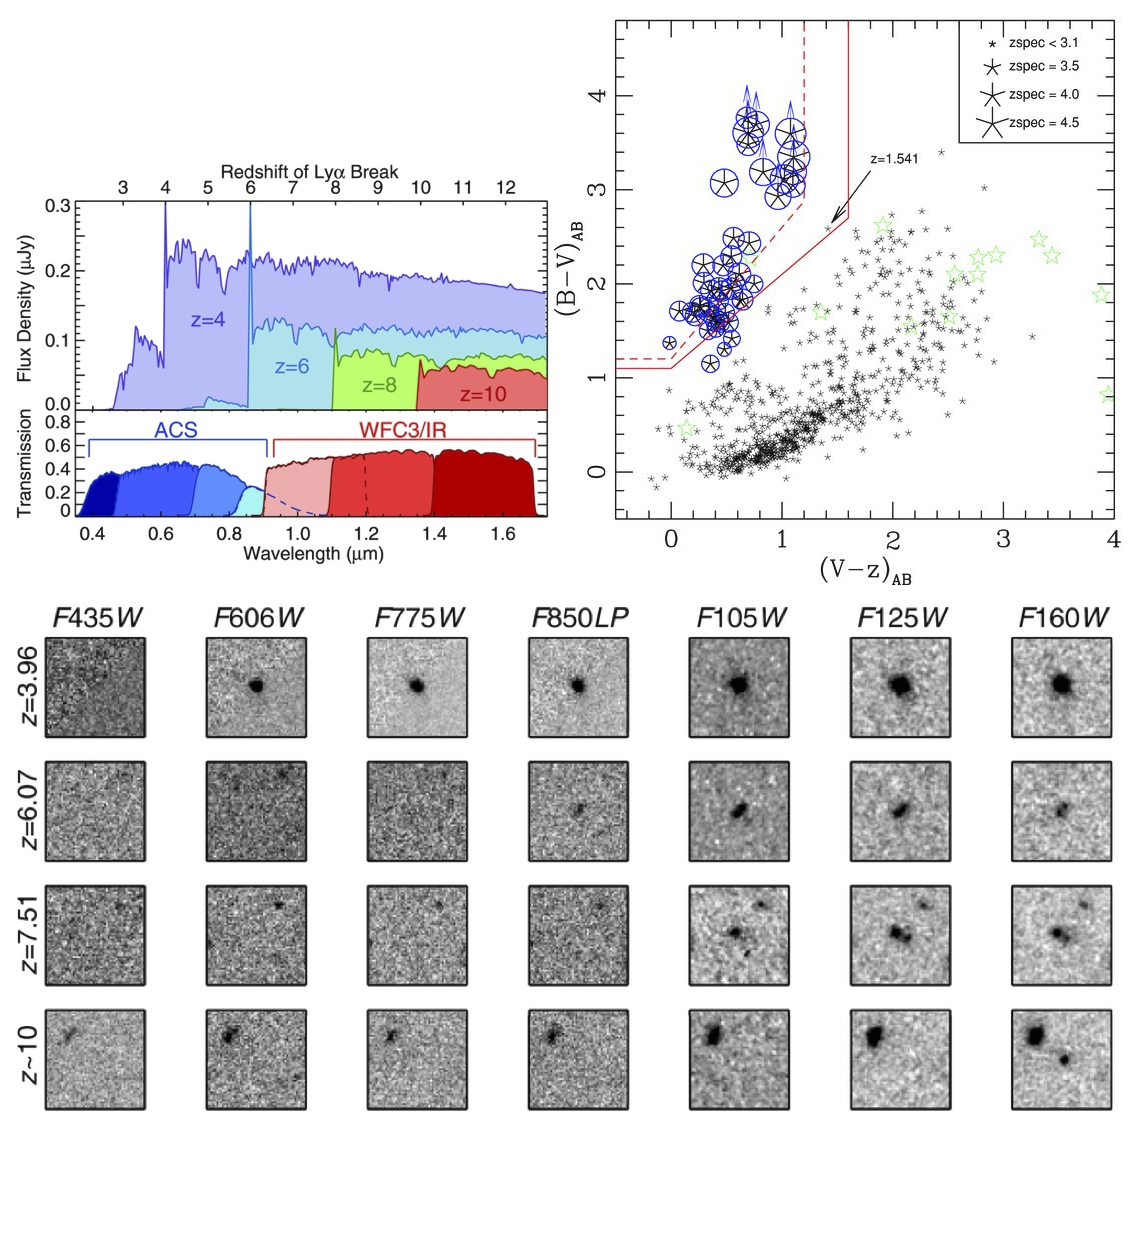
\includegraphics[width=1.0\textwidth]{Chapter1/Figs/Lyman_break_selection.png}
\caption[Selection of Lyman-break galaxies]{Illustration of the selection process for Lyman-break galaxies. The top left part is taken from \cite{2016PASA...33...37F}, and shows model spectra of star-forming galaxies at $z=4$, $z=6$, $z=8$, and $z=10$ together with the transmission curves for seven \textit{HST} filters. The bottom part, also adapted from \cite{2016PASA...33...37F}, consists of cutouts of \textit{HST} imaging showing real candidates in each of the aforementioned filters. It is clear that if the Lyman break lies between two filters, the galaxies show no flux (`drop out') in filters bluer than the Lyman break, but do appear in all redder filters. The top right figure is reproduced from \cite{2009ApJ...695.1163V}, and shows their colour-colour selection of $B$-dropouts (which lie at $3.1<z<4.4$) using the same filterset as the other two subfigures. The black markers indicate spectroscopically confirmed galaxies, with larger symbols denoting higher redshifts up to $z=4.5$. The green $\star$ symbols denote galactic stars, and the red box delineates the colour-colour cuts that were imposed to select $B$-drops. It is noteworthy that the only contamination inside the box consists of a single low-redshift galaxy (flagged by the arrow), thus demonstrating that the colour cuts lead to highly efficient selection.} 
\label{fig:lyman_break}
\end{figure}


For many star-forming galaxies, the Lyman break is strong enough to be observable in broadband imaging, especially if it falls between two filters. Such a galaxy will be visible in all filters redder than the Lyman break, while it will be undetected (it will `drop out') in all bluer filters. Because of this behaviour, such objects are often referred to as \textit{dropout} galaxies, and the first filter longwards of the Lyman break is often referred to as the \textit{detection} filter. Objects with a Lyman break between the $u$-band and $g$-band (or equivalently the $B$-band in other filter sets) are labelled $u$-dropouts. As their observed Lyman break lies between the $u$ and $g$ filter (roughly at $\lambda_{\mathrm{obs}}\simeq\SI{3500}{\angstrom}$, depending on the filter set), their redshift is approximately $z\sim3$. Using the exact same reasoning, $g$-dropouts (sometimes called $B$-dropouts) lie at $z\sim4$, $r$-dropouts (or $V$-dropouts) at $z\sim5$, and $i$-dropouts at $z\sim6$. The dropout mechanism is depicted in Figure \ref{fig:lyman_break}, which illustrates the appearance of Lyman-break galaxies at various redshifts. \par  

The simplest way to select galaxies via their Lyman break involves using colour cuts to select galaxies that show a red colour between the dropout band and the detection band (to confirm a strong Lyman break) and a blue colour between this detection filter and the next reddest band (to select blue star-forming galaxies rather than low-redshift galaxies or stars with intrinsically red colours). This technique is demonstrated in the top right of Figure \ref{fig:lyman_break}. \par 
 
Naturally, it is also possible to find dropout galaxies in a specific redshift range using photometric redshifts. At high redshifts, such a photo-z approach can often essentially be viewed as a form of Lyman-break selection. This is because at $z\gtrsim5$, the Balmer/\SI{4000}{\angstrom} break --- which is generally the second prominent spectral break --- has redshifted beyond the near-infrared. When using only broadband optical and near-IR data, the  Lyman break is therefore the only strong spectral feature that photo-z algorithms can use to estimate the redshift. Throughout this thesis, any galaxy selected via its broadband rest-frame UV colours will be referred to as a \textit{Lyman-break galaxy} (LBG). This includes objects selected via colour-colour cuts as well as via photometric redshifts. \par 

Colour selection methods and photometric redshifts each have their own merits. The colour-cut method is conceptually simple, computationally fast, not affected by specifics in the photo-z code (such as the template set), and highly reproducable. These advantages also make it more straightforward to model contamination and completeness rates for selected LBG samples, which is necessary for some statistical studies (e.g. the luminosity function introduced in Section \ref{subsubsection:photoz_galaxy_evolution} and to be  discussed further in Section \ref{subsubsection:high_redshift_galaxy_evolution}). On the other hand, colour cuts only make use of data in at most three filters, whereas the photo-z approach makes use of the full available dataset. Additionally, as indicated in Section \ref{subsection:methods}, some photometric redshift methods can also constrain certain galaxy properties, as well as output a redshift probability distribution for each source. The latter estimates the probability of potential low-redshift solutions, and also helps to increase the redshift precision (with photometric redshifts the precision at $z\sim6$ is around $\Delta z \sim \pm 0.2\text{--}0.3$, as opposed to $\Delta z \sim0.5$ for colour-cut techniques; \citealt{2016PASA...33...37F}). The history and current status of observational searches for LBGs will be discussed in Section \ref{subsubsection:lyman_break_galaxy_history}, where it will be shown that both photo-zs and colour cuts remain competitive up to the current day. The choice of method therefore largely depends on the research goals and available filtersets for each LBG study, and on the personal preference of the authors. \par  




\subsubsection{Quiescent and dusty high-redshift galaxies}\label{subsubsection:dusty_quiescent}
The selection of LAEs and LBGs described above is based on their rest-frame UV emission, which means that these methods are only sensitive to galaxies with active star formation that is not significantly attenuated by dust. Therefore, these strategies will miss extremely dusty galaxies, as well as passive quiescent galaxies that no longer form stars. \par 

However, an alternative search method that makes use of submillimeter imaging has revealed several highly dust-attenuated galaxies at $z\gtrsim5$ (see e.g. \citealt{2010ApJ...720L.131R,2012Natur.486..233W}). The UV radiation produced by the intense star formation in these extremely reddened objects is almost entirely absorbed by the vast amounts of dust in their interstellar media. This process heats the dust, which then re-radiates its energy at (rest-frame) far-infrared wavelengths. At high redshifts, this emission is shifted into the submillimeter regime, where it can be detected by instruments such as the \textit{Herschell Space Observatory} and the James Clerk Maxwell Telescope.  An in-depth discussion of extremely dusty galaxies is outside the scope of this thesis, but  \cite{2014PhR...541...45C} provide an excellent review for those who are interested in more information. \par 

Regarding quiescent galaxies, there are currently no known secure candidates\footnote{Although it must be noted that \cite{2016PASJ...68...46M} have found a number of uncertain contenders.} of this population at $z\gtrsim5$. While photometric redshifts and colour-colour cuts directed at the Balmer break\footnote{This method works analogously to the Lyman-break colour selection described in Section \ref{subsubsection:lyman_break}.} have yielded a handful of plausible candidates at $z\sim4.5$ \citep{2014ApJ...794...68N,2018MNRAS.473.2098M}, none of these are spectroscopically confirmed. The fact that searches have thus far not returned any convincing results is in fact not unexpected; since galaxies at $z>5$ would have needed to reach quiescence within 1.2 Gyr of the Big Bang, a large population of such objects is very unlikely. If they do indeed exist, the deep near-IR imaging that will soon be available with \textit{JWST} should be able to uncover them \citep{2016PASA...33...37F,2016PASJ...68...46M}. \par




\subsection{Lyman-break galaxies at high redshifts}
Out of all the different types of high-redshift galaxies discussed above, this thesis exclusively concerns itself with Lyman-break sources, for reasons that will be substantiated in Section \ref{section:motivation_high_z}. The rest of the current review of high-redshift science will therefore focus exclusively on this topic. The discussion will cover a brief overview of $z\gtrsim5$ LBG searches in the literature, as well as an outline of several interesting quantities and physical probes that can be studied via these objects. \par 

\subsubsection{Historical overview and state of the art}\label{subsubsection:lyman_break_galaxy_history}
The first attempts to identify distant galaxies by their Lyman break began at the start of the CCD era in the early 1990s \citep{1990ApJ...357L...9G,1993AJ....105.2017S}. These early studies used colour-colour cuts to select $u$-dropouts around $z\sim3$, and the first such candidate was soon spectroscopically confirmed \citep{1994A&A...288..103G}. By the end of the decade, small samples of galaxies were starting to be found around $z\sim5$, with the rapidly developing photo-z techniques providing a valuable tool in this endeavour \citep{1996Natur.381..759L,1999ApJ...513...34F}. A handful of these candidates quickly received spectroscopic confirmation \citep{1998AJ....116.2617S,1998ApJ...505L..95W}.  Nevertheless, larger samples of high-redshift galaxies could not be identified until the development of better red-sensitive instrumentation. After this need was met by new \textit{HST} instruments in the mid-2000s, space-based surveys such as GOODS and the HUDF (see Table \ref{table:space_small_survey} for both) started to unveil samples of more than a hundred $z>5$ galaxy candidates, discovered through either colour-cut or photometric redshift methods \citep{2003MNRAS.342..439S,2004ApJ...600L.103G,2006A&A...449..951G,2006ApJ...653...53B}. One of the first spectroscopic confirmations of a $z\sim6$ candidate followed soon after \citep{2004ApJ...600L..99D}. Around the same time, parallel improvements in terrestrial telescopes enabled significant progress from the ground. Surveys such as the SDF, SDXF (both optical, see Table \ref{table:ground_small_survey}), and UKIDDS (near-IR, idem) prompted the discovery of large samples of high-redshift LBGs from ground-based data, again using both colour cuts and photo-z selection. Although only just over twenty candidates were found at $z>7$ \citep{2009ApJ...706.1136O}, more than a hundred were discovered at $z\sim5$ and $z\sim6$ \citep{2004ApJ...613L...9N,2004ApJ...611..660O,2006MNRAS.372..357M,2006ApJ...653..988Y}. These ground-based searches covered areas of $\sim \SI{1}{\sqdeg}$ --- more than a two-fold increase over GOODS, the largest space-based project at the time. Since larger search areas are more likely to contain rare objects, these ground-based datasets complemented space-based imaging by revealing bright galaxies (<\SI{26.0}{\magab}), which are too uncommon for the relatively narrow surveys from space. \par


The last 10 years brought even further advancements in the selection of LBG samples. From space, improvements in instrumentation led to deeper and wider surveys\footnote{The CANDELS, HUDF09 and HUDF12 data have also been combined into the HXDF, which was introduced in Section \ref{subsubsection:space_based_surveys}.} such as CANDELS (see Table \ref{table:space_small_survey}), HUDF09 (PI: Illingworth, described in e.g. \citealt{2011ApJ...737...90B}), and  HUDF12 \citep{2013ApJS..209....3K}, which together yielded around 3000 $z\sim5$ and 800 $z\sim6$ LBG candidates \citep{2015ApJ...810...71F,2015ApJ...803...34B}. The extreme depths also allowed the selection of several hundred secure candidates out to $z\sim7\text{--}8$ \citep{2015ApJ...810...71F,2015ApJ...803...34B}, and roughly a few dozen\footnote{Among these is an object spectroscopically confirmed at $z=11.1$ \citep{2016ApJ...819..129O}. This galaxy is currently the most distant known source in the universe. As this implies that we are now able to observe a glimpse of the universe just 400Myr after the Big Bang, its discovery can certainly be regarded as a great triumph of extragalactic astronomy.} objects at $z\gtrsim9$ \citep{2013ApJ...773...75O,2014ApJ...786..108O,2015ApJ...803...34B}. Meanwhile, there similarly were significant advances from the ground, with surveys such as CFHTLS, UltraVISTA, and VIDEO (see Table \ref{table:ground_small_survey} for all) covering footprints of $>\SI{1}{\sqdeg}$. Those larger search areas opened up the study of the brightest ($z_{\mathrm{AB}}<25.0$) high-redshift candidates, which will be discussed in more detail shortly. They also revealed several dozen $z\sim7$ candidates \citep{2010A&A...524A..28C,2014MNRAS.440.2810B}, but the vast majority of ground-based objects were discovered at $z\sim5\text{--}6$, with a combined total of hundreds of plausible LBGs at $z\sim6$ \citep{2013AJ....145....4W,2015MNRAS.452.1817B,2009MNRAS.395.2196M} and thousands at $z\sim5$ \citep{2009MNRAS.395.2196M,2010A&A...523A..74V}. The reason why so many more $z\sim5$ candidates have been found compared to $z\sim6$, besides an intrinsic drop in number density with increasing redshift, lies partly in the available datasets. The underlying cause is that secure redshift estimates require detections in at least 2 bands redwards of the Lyman break\footnote{This is necessary to select galaxies with blue intrinsic colours, in order to remove contamination from intrinsically red objects such as dusty galaxies and low mass stars. This requirement applies to both photometric redshift methods and colour cuts, although in the case of photometric redshifts, more detections are additionally useful for providing a better constraint on the fit.}. Since many optical datasets include $i$- and $z$-band data, $r$-dropouts at $z\sim5$ can be found from optical data alone, since they can be detected in both $i$ and $z$. However, additional redder filters are required for $i$-dropouts at $z\sim6$, which means that these searches are restricted by the availability of deep near-IR data. \par 

Up until the current day, colour-cut methods and photometric redshift selection both remain competitive, and the studies mentioned above have used both approaches in roughly equal numbers. Out of all  the LBG candidates that all those searches have identified, more than a hundred $z\gtrsim5$ galaxies have so far been spectroscopically confirmed, mostly at $z<7$  (e.g. \citealt{2005ApJ...626..666M,2009ApJ...695.1163V,2010MNRAS.408.1628S,2011ApJ...743...65J,2012MNRAS.422.1425C,2014ApJ...793..113P,2018MNRAS.479...43K}). \par 

The picture that emerges from this collective body of research is rather impressive. Astronomers are now able to catch a first glimpse of the $z\gtrsim9$ universe, and statistically secure samples of hundreds of $z\sim7\text{--}8$ galaxies are beginning to emerge. The state of the art at $z\sim5$ and $z\sim6$ also contains a wealth of data, with over 1000 and \num{10000} candidates respectively. Nevertheless, despite all this progress, number counts of the brightest ($z_{\mathrm{AB}}<25.0$) LBGs at $z\sim6$ are still relatively low. At the time of writing\footnote{It is possible that the study by \cite{2015ApJ...810...71F} also contains some candidates, but they did not publish apparent magnitudes, and the footprint of their study is almost entirely contained within \cite{2015ApJ...803...34B}, so these results are omitted.}, there are 14 such candidates from a \SI{4}{\sqdeg} ground-based study by \cite{2013AJ....145....4W},  9 from a \SI{1.65}{\sqdeg}  ground-based search by \cite{2015MNRAS.452.1817B}, and approximately\footnote{It must be noted that these galaxies are classified as bright due to their $Y_{105}<25.0$ magnitude, as \cite{2015ApJ...803...34B} did not publish $z$-band magnitudes. Therefore it is possible that the actual number of $z<25.0$ slightly deviates from this number.} 13 from \SI{0.26}{\sqdeg} from a predominantly space-based investigation by \cite{2015ApJ...803...34B}. After accounting for duplicates, those studies contain a relatively modest total of 32 unique $z_{\mathrm{AB}}<25.0$ candidates. A combination of deep optical and near-IR imaging over a large area of several square degrees would be required to improve these numbers. \par





\subsubsection{The importance of Lyman-break galaxies for high-redshift galaxy evolution studies}\label{subsubsection:high_redshift_galaxy_evolution} %CALL THIS 'THE IMPORTANCE OF HIGH-REDSHIFT LYMAN-BREAK GALAXIES'
Samples of high-redshift Lyman-break galaxies from the last 20 years have contributed enormously to the study of galaxy evolution at early times. This is an extremely rich field with a vast quantity of ongoing research, and a detailed summary of recent developments can be found in the reviews by  \cite{2013ASSL..396..223D} and \cite{2016PASA...33...37F}. However, in order to provide a brief illustration of the interesting science that can be achieved with high-redshift LBGs, this section highlights\footnote{Since the target of this thesis is bright LBGs (for reasons that will be presented in Section \ref{subsection:conclusion_high_z_intro} shortly), the narrative will focus predominantly on those objects. More information on all the science that can be achieved with fainter sources can be found in e.g. \cite{2013ASSL..396..223D} and \cite{2016PASA...33...37F}.} a number of interesting galaxy properties that can be investigated through these objects. \par


\paragraph{UV luminosity function} One of the most straightforward quantities to measure from samples of Lyman-break galaxies is the UV luminosity function (LF; briefly introduced in Section \ref{subsubsection:photoz_galaxy_evolution} earlier), which quantifies the number density of galaxies per unit of comoving volume per unit of absolute rest-frame UV luminosity (usually $M_{\SI{1600}{\angstrom}}$ or $M_{\SI{1500}{\angstrom}}$). The reason why LBG LFs are usually measured in the ultraviolet is because the deepest survey data generally exists at optical and near-IR frequencies, which for LBG redshifts of $z\gtrsim3$ translates to the rest-frame UV.  \par


The UV luminosity function is an extremely useful measure, as it provides insights into physical processes in the universe. For instance, it can be used to estimate the total number of ionizing UV photons produced by galaxies, and thus whether galaxies could have been the main contributor to the reionisation of the intergalactic medium \citep{2010Natur.468...49R,2013ApJ...768...71R}. Furthermore, because it tracks light from newly formed blue stars, the UV luminosity function can also be converted into the cosmic star formation rate density, which quantifies the total amount of star formation occurring in the universe at a given redshift. Studying the variation of the cosmic star formation rate with redshift has started to provide some insights into the growth of stellar mass, and when its build-up commenced \citep{2013ApJ...763L...7E,2014ARA&A..52..415M,2015ApJ...803...34B,2015ApJ...810...71F}. Lastly, because it can be computed fairly easily from both theory and observations, the LF is a useful probe for some of the physical processes that drive galaxy evolution.  A comparison between the shape of the luminosity function (from observations) and the halo mass function of the underlying dark matter haloes (from simulations) can provide clues as to the physical mechanisms at play. At both the bright and the faint end, the luminosity function at most redshifts has generally been found to lie below what would be expected on the basis of galaxy halo masses. This suggests that the conversion of gas (the abundance of which roughly scales with the dark matter halo mass) into starlight is less efficient in both the brightest and the faintest galaxies. It is believed that this phenomenon is caused primarily by processes that heat the interstellar medium and expel gas from galaxies, which subsequently suppresses their star formation. The primary candidates for causing this disruption include supernova feedback and stellar winds at the faint end, and AGN feedback at the bright end \citep{2003ApJ...599...38B,2008MNRAS.391..481S,2015ARA&A..53...51S}.  \par


\begin{figure}[t] 
\centering    
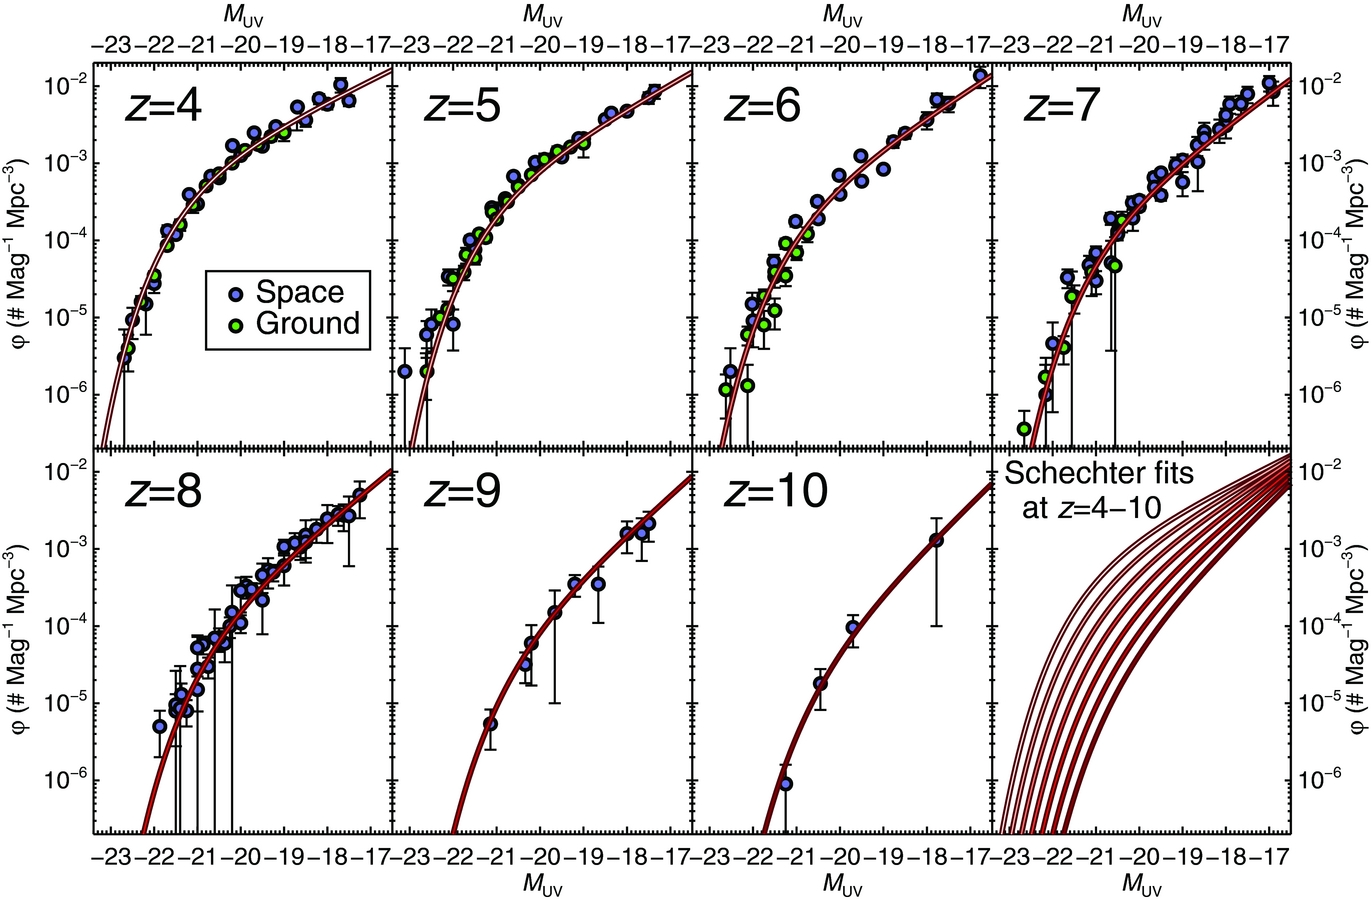
\includegraphics[width=1\textwidth]{Chapter1/Figs/Luminosity_functions.png}
\caption[Luminosity functions at \texorpdfstring{$4<z<10$}{TEXT}]{A compilation of UV luminosity functions created by \cite{2016PASA...33...37F}, constructed from recent samples of LBGs in various redshift bins. The dots are data points from several space-based and ground-based studies (sources are listed in \citealt{2016PASA...33...37F}), and the red curves are reference Schechter function \citep{1976ApJ...203..297S} fits to these data points (computed as described in \citealt{2016PASA...33...37F}).}
%It is clear that at $z\sim4$ and $z\sim5$ the luminosity functions are well constrained, with low scatter and low uncertainties, while at $z\gtrsim7$ the uncertainties are larger due to the smaller sample sizes. The situation at $z\sim6$ is mixed, with low uncertainties at the faint end\footnote{The scatter in the faint end at $z\sim6$ is caused by a difference in the normalisation factor due to systematic differences in the LF computation between studies (see \cite{2016PASA...33...37F})} and larger error bars at the bright end. These large uncertainties are predominantly caused by the small (<50) sample size of these bright objects (see Section \ref{subsubsection:lyman_break_galaxy_history}).
\label{fig:luminosity_functions}
\end{figure}


To study the changes in all these physical processes over time, UV luminosity functions are usually computed from samples of LBGs at various redshifts. In order to be able to reach secure conclusions, it is important that these functions are well measured. To illustrate to what extent current data provide adequate constraints, Figure \ref{fig:luminosity_functions} shows a compilation of LF data points from recent observational studies at $4<z<10$. It is clear that the measurements at $z\sim4$ provide fairly solid constraints, thanks to the generous samples of LBGs used to obtain these data points. Similarly, it is evident that the same largely applies at $z\sim5$ (with the exception of the extreme bright end, which shows some large error bars mainly due to space-based studies having low number counts in this regime). And conversely, it is also apparent that the results at $z\gtrsim7$ are generally rather uncertain, primarily due to the small sample sizes. The data points at $z\sim6$, on the other hand, present a more mixed situation. At the faint end, the uncertainties are small, although there does exist some scatter (likely originating from systematic differences in the LF computation between studies; \citealt{2016PASA...33...37F}). The bright end likewise suggests some tension between studies, but critically shows much larger error bars in addition to that. Those big uncertainties are predominantly caused by the small number of known bright galaxies, an issue which has previously been noted in Section \ref{subsubsection:lyman_break_galaxy_history}. Better constraints in this regime would be valuable, since the bright end around $z\sim6$ also happens to be especially interesting scientifically. This is because there are indications that the aforementioned drop in bright sources compared to the halo mass function, which is known to exist at lower redshifts (e.g. \citealt{2010A&A...523A..74V}), may have commenced around this time \citep{2014MNRAS.440.2810B,2015MNRAS.452.1817B}. This could indicate the start of processes that suppress star formation (such as the beginning of AGN activity), or the onset of dust build-up that obscures some of the stellar UV radiation (see \citealt{2012ApJ...756..164F,2014ApJ...793..115B,2014MNRAS.440.3714R}). \par 


\paragraph{Other galaxy properties}
In addition to the UV luminosity function, there are several other important physical attributes that can be studied with the help of high-redshift LBGs. A major one of these is their stellar masses, which can be probed if mid-IR \textit{Spitzer Space Telescope} data is available  \citep{2006ApJ...651...24Y,2009ApJ...697.1493S,2010ApJ...719.1250F,2011ApJ...735L..34G}. Such imaging captures the rest-frame optical emission, which, in contrast to the rest-frame UV, is sensitive to lower-mass stars that may make up the bulk of galaxy mass. As well as for its own sake, stellar mass has been used to study the amount of star formation in a galaxy per unit of stellar mass (the specific star formation rate; \citealt{2013ApJ...763..129S,2014ApJ...781...34G,2015ApJ...799..183S}) and the dependence of galaxy stellar masses on the underlying dark matter halo mass \citep{2009MNRAS.395.2196M,2013ApJ...770...57B,2015ApJ...814...95F}. Dust attenuation is another interesting property that is being studied, as there is a reasonable amount of evidence that out to $z\sim7$ the brightest galaxies already contain an appreciable amount of dust (displaying reddening of $E(B-V)\sim 0.1\text{--}0.15$; \citealt{2012ApJ...754...83B,2014ApJ...793..115B,2012ApJ...756..164F,2014MNRAS.440.3714R,2015ApJ...814...95F}). Finally, some authors have also begun to make small steps to measure the evolution of galaxy sizes \citep{2010ApJ...709L..21O,2013ApJ...765...68H,2013AJ....145....4W,2014MNRAS.440.2810B}. \par

Spectroscopic follow-up of high-redshift LBG candidates can also provide interesting physical insights, since spectra can  be used to measure the possible presence and strength of the Lyman-$\alpha$ emission line. This can provide constraints on reionisation: if galaxies beyond a certain redshift show an average reduction in their Lyman-$\alpha$ flux, this could signal the presence of increased neutral hydrogen in the IGM (and hence incomplete reionisation). Recent studies indicate that such a drop in Lyman-$\alpha$ has indeed been observed around $z>6$ \citep{2010MNRAS.408.1628S,2011ApJ...743..132P,2013Natur.502..524F,2014ApJ...793..113P}, which agrees with the current consensus that reionisation ended around $z\approx6$. The specifics of how the reduction in Lyman-$\alpha$ at $z>6$ can be converted into particular details about the progression of reionisation are currently the topic of active debate, and there are some tensions between theory and observation (see e.g. the reviews by \citealt{2014PASA...31...40D} and \citealt{2016PASA...33...37F}, and references therein). While spectroscopy at $z>6.5$ would provide the most useful constraints, this is challenging with most instruments due to the dramatic reduction in the sensitivity of optical spectrographs at the extreme red end. However, spectra of $z\approx6$ galaxies are easier to obtain and would also be useful. For instance, galaxies at $z\approx6$ can be used to extrapolate the Lyman-$\alpha$ equivalent width and escape fraction at $z>6.5$ in the absence of neutral hydrogen \citep{2009ApJ...697.1493S,2011ApJ...728L...2S}. This baseline can then be compared to the observed signature from real $z>6.5$ galaxies to estimate how much (not-yet-ionised) neutral hydrogen gas is present in the IGM. There is evidence that the Ly$\alpha$ escape fraction and equivalent width decrease with luminosity, but for the brightest sources the uncertainties on this hypothesis are still large due to the small number counts \citep{2009ApJ...697.1493S,2011ApJ...728L...2S,2012MNRAS.422.1425C}. More spectra of luminous $z\approx6$ objects would therefore be useful. At these great distances, bright galaxies are also more likely to yield usable spectra, making them very suitable targets.  \par


\subsection{Conclusion on high-redshift galaxies}\label{subsection:conclusion_high_z_intro}
In the review above, which focused primarily on Lyman-break galaxies, we have witnessed some key developments in recent high-redshift galaxy evolution studies. Along the way, the discussion presented a strong case in favour of collecting larger samples of the brightest ($z_{\mathrm{AB}}<25.0$) galaxies at $z\sim6$ in particular. For these objects, it was found that the current sample sizes are still small, which leads to large uncertainties on statistical properties. We observed several areas where bright LBG candidates would be valuable for future science. First and foremost, they are required to better constrain the bright end of the luminosity function, which can provide interesting clues as to the onset of AGN activity or dust build-up in the early universe. On top of that, they can also be used to investigate other physical properties, such as galaxy stellar mass and dust content. Finally, if spectra can be obtained, the Lyman-$\alpha$ emission of bright sources can help to provide further constraints on reionisation. \par 

The issue with the small number counts of known bright galaxies is largely caused by the relatively modest footprints of previous optical+near-IR surveys, which did not cover a large enough deep area to find substantial numbers of these rare sources. However, with an effective search area of \SI{4.9}{\sqdeg} ($7.5\sigma$ depths of $z_{\mathrm{AB}}<25.0$), the new optical+near-IR catalogue presented in this thesis offers the largest deep search area to date. Since its footprint only partially overlaps with the previous largest \SI{4}{\sqdeg} study by \cite{2013AJ....145....4W}, it
can provide an appreciable increase in potential sources. Armed with this new dataset, the third part of this thesis thus tackles the important task of identifying additional bright high-redshift Lyman-break galaxies. The largest scientific potential lies in sources at $z\sim6$; but since the dataset is also suitable for objects at $z\sim5$ those sources are also investigated, as we have seen that the extreme bright end of the LF at that redshift does still show considerable uncertainties. The high-redshift samples from these searches will be very valuable for future studies, for instance to help address some of the open questions regarding galaxy properties mentioned in the previous paragraph and Section \ref{subsubsection:high_redshift_galaxy_evolution}. \par




\section{Thesis outline}
Altogether, the current chapter has covered three important and related research areas in contemporary astronomy: surveys, photometric redshifts, and high-redshift galaxies. Each of these topics corresponds to one chapter of this thesis, and the main aims of each part have already been identified in the intermediary conclusions of each section (i.e. Sections \ref{subsection:conclusion_surveys_intro}, \ref{subsection:conclusion_photoz_intro}, and \ref{subsection:conclusion_high_z_intro}). A more detailed structural outline of this thesis is given below: 


\begin{itemize}
    \item \textbf{Chapter \ref{chapter:catalogue}} will address the creation of a \textbf{combined optical and near-infrared source catalogue}. The first section of this chapter will introduce the datasets for this thesis, which consist of the optical ($grizY$) Dark Energy Survey (DES) deep fields, the near-IR ($ZYJHK_{s}$) Vista Deep Extragalactic Observations (VIDEO) survey, and a catalogue of publicly available spectroscopic redshifts for a subset of these sources. The second section will then describe the process of combining the DES and VIDEO datasets into a single multiwavelength catalogue. This is achieved by creating a pipeline that extracts VIDEO forced photometry directly from the imaging and merges it with pre-existing DES collaboration catalogues. The third section will address accuracy verification for the resulting combined \DESVIDEO catalogue, and conclude with an overview of the final photometric data product.
    
    \item \textbf{Chapter \ref{chapter:photometric_redshifts}} will discuss the computation of \textbf{photometric redshifts for the ($grizZYJHK_{s}$) \DESVIDEO catalogue}. The first part will present the template fitting method \texttt{LePHARE} as the choice of code, and describe the working of this algorithm together with its various options and the relevant template SEDs. The second part will then introduce various \texttt{LePHARE} configurations for testing different templates, \texttt{LePHARE} options, and photometry. Each setup is used to compute photo-zs for a subset of \DESVIDEO objects with spectroscopic redshifts, and the photo-z performance of these test runs is assessed via a number of accuracy metrics that capture the difference between photometric and spectroscopic redshift. The primary purpose of this analysis is to identify the most suitable configuration to compute redshifts for the high-redshift search in Chapter \ref{chapter:high_redshift_candidates} (see below), but the discussion will also address the implication of the test results for general photo-z research. The final part of the chapter will then focus on  applying the chosen configurations to the full \DESVIDEO catalogue. This section will also discuss finding an appropriate star-galaxy separation strategy to filter out nonsensical photo-zs from stars, before finally presenting the final redshifts for all galaxies in the \DESVIDEO dataset. 
    
    \item \textbf{Chapter \ref{chapter:high_redshift_candidates}} will describe the \textbf{search for bright $\mathbf{z\sim5}$ and $\mathbf{z\sim6}$ Lyman-break galaxies in the \DESVIDEO catalogue}. The first part will discuss identifying a suitable strategy to select a sample of $m_{\mathrm{AB}} < 25.0$ candidate LBGs at $z\sim5$ and $z\sim6$, detailing the three selection rounds used in this search. The second part will then present the resulting final LBG sample, and compare the outcomes to other studies in the literature. 
\end{itemize}

%!TEX root = ../thesis.tex
%*******************************************************************************
%****************************** Second Chapter *********************************
%*******************************************************************************
\renewcommand{\overbar}[1]{\mkern 1.5mu\overline{\mkern-1.5mu#1\mkern-1.5mu}\mkern 1.5mu}


\makeatletter
\let\ftype@table\ftype@figure
\makeatother

\DeclareUrlCommand\ULurl{%
  \renewcommand\UrlFont{\ttfamily\color{blue}}%
  \renewcommand\UrlLeft{\uline\bgroup}%
  \renewcommand\UrlRight{\egroup}}


\chapter{Combined \DESVIDEO catalogue}\label{chapter:catalogue}

\ifpdf
    \graphicspath{{Chapter2/Figs/Raster/}{Chapter2/Figs/PDF/}{Chapter2/Figs/}}
\else
    \graphicspath{{Chapter2/Figs/Vector/}{Chapter2/Figs/}}
\fi

Astronomy is undoubtedly in a data driven golden age of surveys. Chapter \ref{chapter:introduction} described how, spurred by technological advances in imaging and data processing technology, this revolution has enabled the efficient discovery of millions of galaxies in deep fields. Moreover, the observation of these sources over many parts of the electromagnetic spectrum has opened up a wide range of tracers for galaxy activity. With studies starting to constrain galaxy properties all the way into the first billion years of cosmic evolution, further opportunities for progress now lie in the direction of deeper surveys and larger areas. With a combination of optical and near-infrared imaging over the largest deep ($z_{\mathrm{AB}}<24.9$, $K_{s}<23.8$) area to date, this thesis tackles the latter strategy.  \par

The process of merging optical data from the Dark Energy Survey (DES) and near-infrared data from the VISTA Deep Extragalactic Observations (VIDEO) survey into a combined \DESVIDEO catalogue forms the topic of the current chapter. The first section will introduce the core DES and VIDEO datasets, and present the spectra that are used as auxiliary data in later chapters. After that, the discourse will turn to the forced photometry process that combines the DES and VIDEO data, as well as various data checks to confirm the validity of the resulting combined catalogue. \par



%********************************** %First Section  **************************************
\section{Data}
\subsection{The Dark Energy Survey (DES)}
\subsubsection{Overview}
The Dark Energy Survey (DES; \citealt{2005IJMPA..20.3121F,2018ApJS..239...18A}) is an optical photometric survey with the primary scientific goal of probing the nature of dark energy by measuring the history of cosmic expansion to high precision. It achieves this through four independent probes: supernova distances, galaxy cluster counts, weak gravitational lensing and galaxy angular clustering. The last three quantities are measured by the so-called \textit{wide-field} survey, which covers \SI{5000}{\sqdeg} in five optical $grizY$ filters. This imaging provides the required morphological information and number counts, which can be tracked over cosmic time via photometric redshifts, similarly computed from the broadband data.  The \textit{time-domain} survey contains the supernova part of DES. This transient component covers \SI{27}{\sqdeg} imaged at regular seven-night intervals in $griz$ filters, in order to detect Type Ia supernov\ae{} and measure their lightcurves. Because Type Ia supernov\ae{} are standard candles, measuring their light output provides an independent distance measurement to track the expansion of the universe, and thus constrain dark energy. \par 



\subsubsection{Data collection}\label{subsubsection:data_collection}

\begin{figure}[htbp] 
\centering    
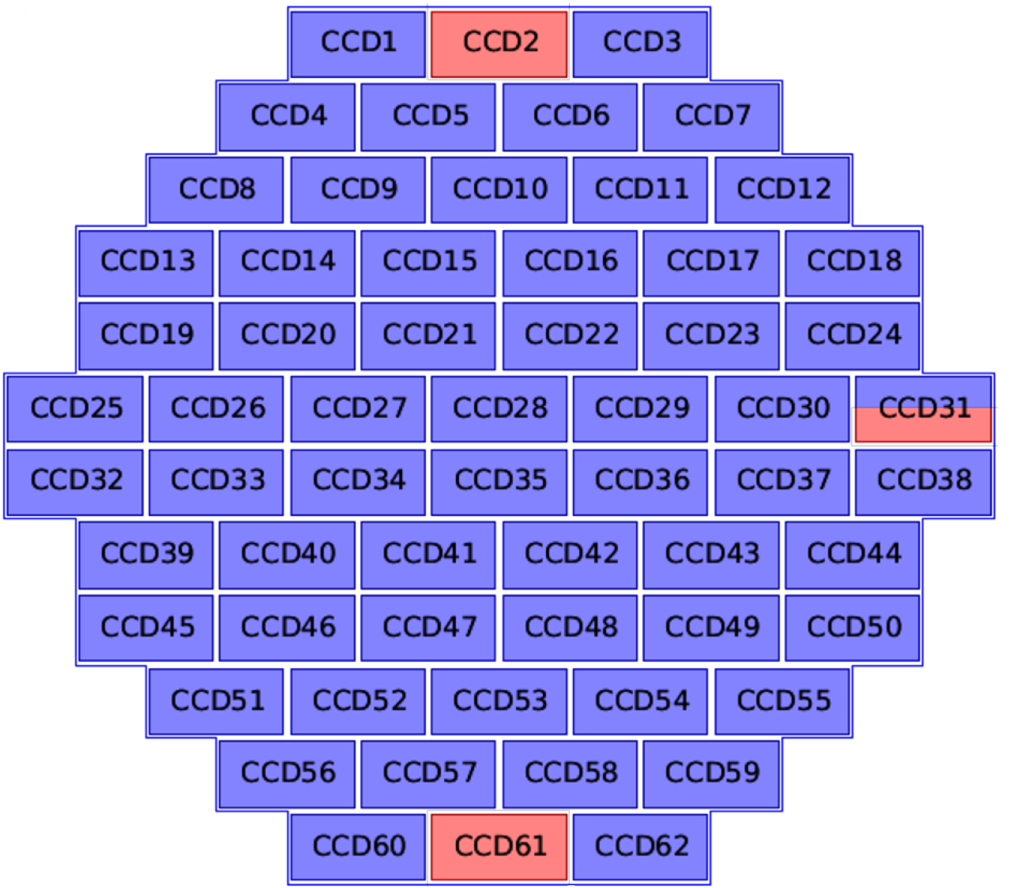
\includegraphics[width=0.6\textwidth]{DECAM_CCD.jpg}
\caption[DECam focal plane]{Focal plane of the Dark Energy Camera (DECam), consisting of 62 CCDs arranged in a hexagonal pattern covering a \SI{3}{\sqdeg} field-of-view. North is displayed at the top and east is on the right. The red sections (CCD 2, CCD 61, and half of CCD 31) were not functional for most of the Year 1 observations used in this catalogue, and data from these regions is not used in this thesis. \textit{Image credit:} \cite{2018ApJS..239...18A}.}
\label{fig:DECAM}
\end{figure} 


Imaging for DES has been obtained with the specially constructed Dark Energy Camera (DECam; \citealt{2015AJ....150..150F}), mounted on the Blanco 4-m telescope at the Cerro Tololo Inter-American Observatory. Containing the latest wide-field imaging technology, DECam has a \SI{3}{\sqdeg} field of view and a 570 megapixel CCD camera, made up of 62 arrays arranged in a hexagonal pattern as per Figure \ref{fig:DECAM}. The camera has a resolution of \SI{0.263}{\arcsec.pix^{-1}}. Observations for DES were conducted using the five main DECam broadband filters $grizY$, of which the transmission curves are plotted in Figure \ref{fig:filters} and wavelength coverage provided in Table \ref{table:effective_wavelengths}. \par



The survey saw first light in September 2012, and observations for the full survey were carried out between August 2013 and January 2019. Over these six years, the \SI{5000}{\sqdeg} wide-field area was covered several times in all five $grizY$ filters to create the footprint shown in Figure \ref{fig:DES_footprint}. In the wide component, each (hexagonal) exposure in the same field was offset by roughly half the focal plane radius, such that objects were observed by different CCDs in each visit. This dithering strategy minimises the effects from inhomogeneities in the DECam apparatus and enhances the photometric calibration. Every year, the exposures collected up to that point are co-added to produce deep imaging (see \citealt{2018ApJS..239...18A} and \citealt{2018PASP..130g4501M} for details), which will reach the final survey depths after the full five years' worth of data have been processed. \par 



\begin{figure}[!pht] 
\centering    
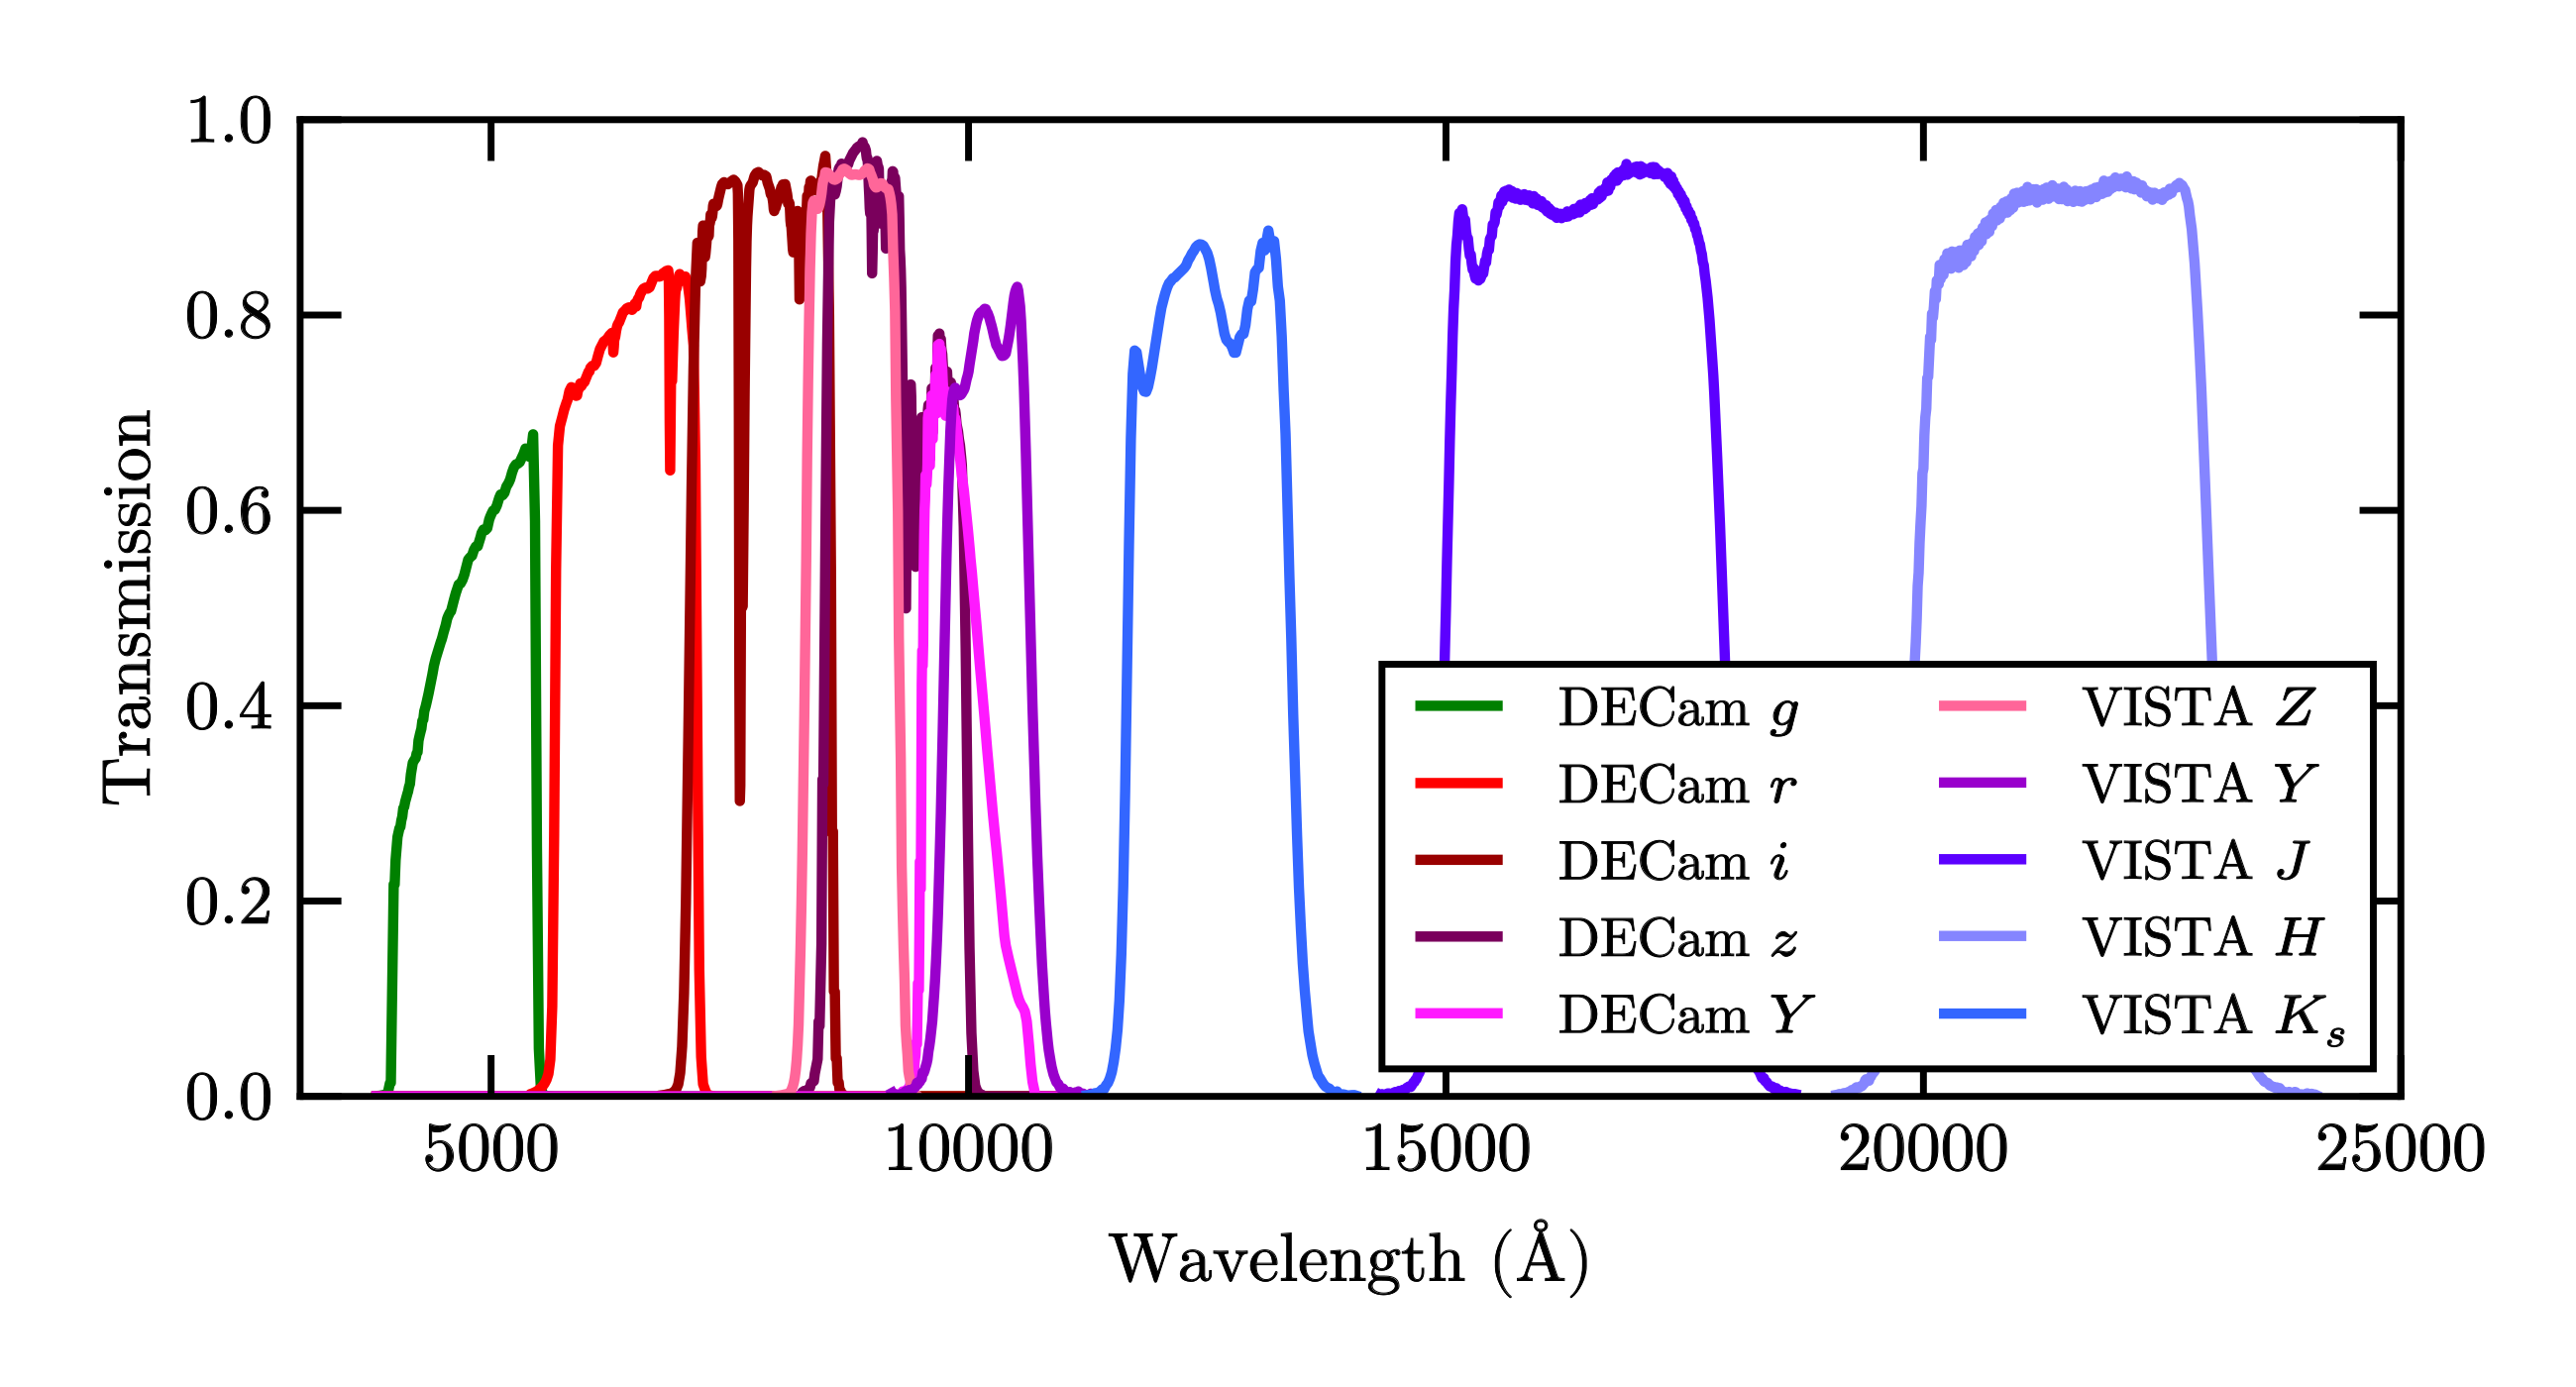
\includegraphics[width=0.95\textwidth]{filters.png}
\caption[DES and VIDEO filter transmission curves]{Transmission curves for the optical to near-infrared filters used in this project from DES (DECam) and VIDEO (VISTA). These plots show the relative total throughput, including the effects of the atmosphere and quantum efficiency of the detector.}
\label{fig:filters}
\end{figure}

\begin{table}[!phb]
\centering
\textsc{Wavelength coverage of filters} \\
\vspace{0.1em}
\footnotesize
\begin{tabular}{lcccclccc}
\toprule\toprule
\multicolumn{4}{c}{\textsc{DECam}} & &  \multicolumn{4}{c}{VISTA}  \\
Filter & $\lambda_{\mathrm{cent}}$ (\si{\angstrom}) & $\lambda_{\mathrm{min}}$ (\si{\angstrom}) & $\lambda_{\mathrm{max}}$ (\si{\angstrom}) & & Filter & $\lambda_{\mathrm{cent}}$ (\si{\angstrom}) & $\lambda_{\mathrm{min}}$ (\si{\angstrom})  & $\lambda_{\mathrm{max}}$ (\si{\angstrom}) \\
\midrule
$g$ & 4730 & 3980 & 5480 & & $Z$ & 8780 & 8285 & 9255 \\ 
$r$ & 6420 & 5680 & 7160 & & $Y$ & 10200 & 9735 & 10665 \\
$i$ & 7840 & 7100 & 8570 & & $J$ & 12520 & 11660 & 13380 \\
$z$ & 9260 & 8500 & 10020 & & $H$ & 16450 & 14995 & 17905 \\
$Y$ & 10090 & 9530 & 10650 & & $K_{s}$ & 21470 & 19925 & 23015 \\
\bottomrule
\end{tabular}
\vspace{1em}
\caption[Wavelength coverage of broadband filters]{The central wavelengths $\lambda_{\mathrm{cent}}$, and left and right edges $\lambda_{\mathrm{min}}$ and $\lambda_{\mathrm{max}}$ for all DECam and VISTA filters used in this thesis. $\lambda_{\mathrm{min}}$ and $\lambda_{\mathrm{max}}$ are defined as the wavelength at which 50\% relative transmission occurs. Each central wavelength is a simple interpolation between $\lambda_{\mathrm{min}}$ and $\lambda_{\mathrm{max}}$.}
\label{table:effective_wavelengths}
\end{table} 




\begin{figure}[htb] 
\centering    
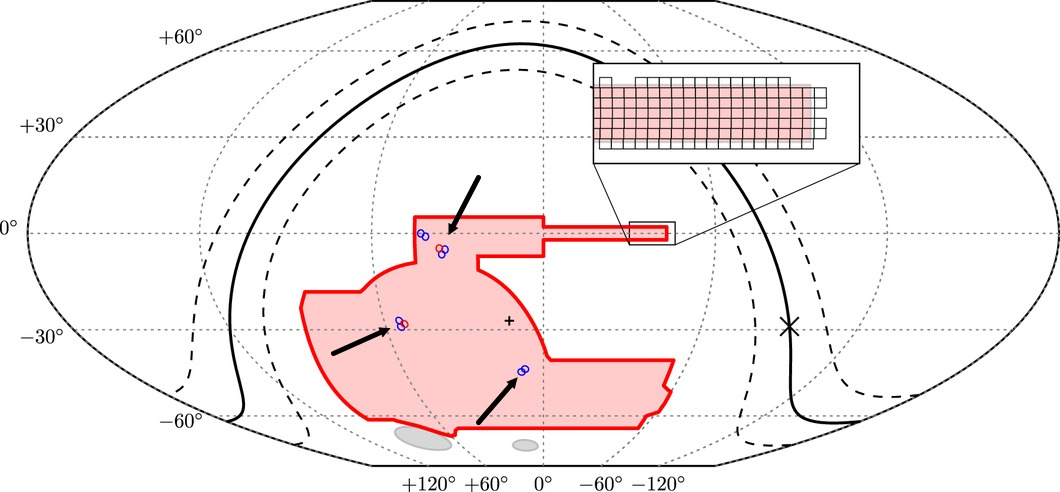
\includegraphics[width=1.0\textwidth]{Chapter2/Figs/DES_footprint_arrows.jpg}
\caption[Map of the DES footprint]{Map of the Dark Energy Survey (DES) area in celestial coordinates. The \SI{5000}{\sqdeg} wide-field survey is shown in red. The eight shallow supernova (SN) fields are displayed as blue circles, and the two deep SN fields are displayed as red circles. The catalogue created in this thesis is based on the eight most southern SN fields, denoted by the black arrows. The other two SN fields around the celestial equator are not included in this work, because they do not overlap with any near-infrared data of a suitable depth. The black line presents the Milky Way plane, and the Galactic center and Galactic pole are marked by a cross ($\times$) and a plus ($+$) respectively. The inlay shows the way the wide-field survey is cut up into co-add tiles by the DESDM processing pipeline. \textit{Image credit:} \cite{2018ApJS..239...18A}}
\label{fig:DES_footprint}
\end{figure}


The time-domain survey has employed a different observing strategy. In this component, the target fields were observed frequently using $griz$ filters only, at regular intervals approximately seven nights apart \citep{2015AJ....150..172K}.  Similarly to the wide-field survey, these exposures are then co-added. These co-added images constitute the so-called DES deep fields, interchangeably referred to as supernova fields. As they contain a substantially higher number of exposures per unit area, these fields reach $\sim\SIrange{1}{2}{\magab}$ deeper in $griz$ compared to the rest of DES. $Y$-band coverage in the supernova fields is provided by the (shallower) wide-field data. In contrast with the main survey, where subsequent exposures in the same field were dithered to achieve maximum data uniformity, each supernova pointing in a given field is the same to within a few arcseconds \citep{2015AJ....150..172K}. While this is useful for supernova science, since it makes it easy to identify if an object has changed in brightness between pointings, an unfortunate side effect of this observing strategy is the presence of chip gaps in the co-added images. These chip gaps originate from the arrangement of the DECam CCDs, which, as demonstrated in Figure \ref{fig:DECAM}, are not perfectly adjacent (see Figures \ref{fig:depth_es1}, \ref{fig:depth_xmm}, and \ref{fig:depth_cdfs} for a visible imprint of these gaps in the data). To compensate for the lack of dithering, the supernova survey used a special photometric calibration strategy, detailed in \cite{2015AJ....150..172K}. \par



The DES deep fields, referred to as the \texttt{DFULL} dataset by the DES collaboration,  form the optical component of the \DESVIDEO catalogue presented in this thesis. To illustrate the positions of the fields, their locations are superimposed on the wide-area DES footprint in Figure \ref{fig:DES_footprint}. It is useful to emphasise that, even though DES has observed a total of ten supernova fields, this thesis includes only eight fields (E1, E2, X1, X2, X3, C1, C2 and C3). The other two (S1 and S2, overlapping the SDSS Stripe 82; \citealt{2007ApJS..172..634A, 2009ApJS..182..543A}) were disregarded due to a lack of available deep near-infrared data. Central coordinates for the eight fields in this thesis are provided in Table \ref{table:fields}. The `E' fields overlap the ELAIS-S1 field \citep{1999MNRAS.305..297G}, the `X' fields overlap the \textit{XMM}–\textit{Newton} Large-Scale Structure field (XMM-LSS; \citealt{2004JCAP...09..011P}), and the `C' fields overlap the \textit{Chandra} Deep Field South (CDF-S; \citealt{2011ApJS..195...10X}). Since each supernova field extends over approximately \SI{3}{\sqdeg} (the field-of-view of a single pointing), the area coverage of the optical data available for this thesis totals around \SI{24}{\sqdeg}. \par





\begin{table}[!htbp]
\centering
\textsc{DES deep (supernova) fields} \\
\vspace{0.1em}
\footnotesize
\begin{tabular}{clccc}
\toprule\toprule
DES name & Field & R.A. (J2000) & DEC (J2000) & Type \\
\midrule
E1 & ELAIS-S1  & 00:31:29.86 & -43:00:34.6 & shallow \\
E2 & ELAIS-S1  & 00:38:00.00 & -43:59:52.8 & shallow \\
X1 & XMM-LSS  & 02:17:54.17 & -04:55:46.2 & shallow \\
X2 & XMM-LSS  & 02:22:39.48 & -06:24:43.6 & shallow \\
X3 & XMM-LSS  & 02:25:48.00 & -04:36:00.0 & deep \\ 
C1 & CDF-S  & 03:37:05.83 & -27:06:41.8 & shallow \\
C2 & CDF-S  & 03:37:05.83 & -29:05:18.2 & shallow \\
C3 & CDF-S  & 03:30:35.62 & -28:06:00.0 & deep \\
\bottomrule
\end{tabular}
\vspace{1em}
\caption[Coordinates of the DES deep fields]{Central coordinates of the eight \SI{3}{\sqdeg} DES deep fields, also referred to as supernova fields. The two so-called deep supernova fields X3 and C3 contain more exposures and are  $\sim\SI{1}{\magab}$  deeper than the shallow fields.}
\label{table:fields}
\end{table}



It is important to point out that this thesis exclusively uses of data from the first year of observations (see \citealt{2014SPIE.9149E..0VD}). This dataset was released internally to the DES collaboration as \texttt{Y1A1} \citep{2018ApJS..235...33D} and is a subset of the data published in the first public data release \texttt{DR1} (which covers all the first three years; \citealt{2018ApJS..239...18A}). The reason for including only the \texttt{Y1A1} data is that at the time the work in this thesis was carried out, data from later years was not yet available due to processing delays. Fortunately, the \DESVIDEO catalogue production pipeline presented in this thesis largely uses automated processes, so it would be straightforward to extend this work to incorporate data from any later releases. \par 




\subsubsection{Data reduction}\label{subsubsection:data_reduction}
After the Year 1 exposures had been taken, the data was processed and combined into deep co-added images. Before this could occur, all DES exposures were required to pass preliminary quality checks on the point spread function (PSF) and signal-to-noise ratio, detailed in  \cite{2018ApJS..235...33D}. The exposures that passed these quality control standards were then processed by the DES data management system (DESDM;  \citealt{2011arXiv1109.6741S, 2012SPIE.8451E..0DM, 2018PASP..130g4501M}), with the aim of producing science ready imaging. The details of this procedure are described at length in \cite{2018ApJS..235...33D} for the \texttt{Y1A1} data used in this thesis. During data processing, the DESDM pipeline removed instrumental signatures from the telescope and DECam setup, and performed masking of artefacts including bright stars, cosmic rays, and fast-moving transients such as satellites and meteors. The DESDM algorithm also created weight images. These weight planes were generated for each individual exposure based on the inverse variance of a flat field image, as this variance captures the Poisson noise and read noise of the instrument. Weight values were then set to zero for all saturated pixels in bright stars, and for masked pixels from artefacts and transients.  \par


The processed exposures then underwent a second round of quality control cuts, intended to blacklist and remove individual CCD images with severe imaging artefacts from phenomena such as scattered light from bright stars, or airplane and meteor trails. For \texttt{Y1A1}, only 1\% of CCD images {were} discarded in this way, and the details of this procedure can once again be found in \cite{2018ApJS..235...33D}. DESDM then produced image co-adds of all approved images, obtained from the weighted average of all overlapping images (using the weight maps described above). The co-addition was performed using \texttt{SWarp} \citep{2002ASPC..281..228B,2010ascl.soft10068B}, which remapped all pixels onto a uniform grid with a pixel scale of \SI{0.263}{\arcsec.pix^{-1}}. This grid was then cut up into co-add tiles of $\num{10 000 x 10 000}$ pixels (covering $\SI[product-units = repeat]{0.73 x 0.73}{deg}$), as illustrated in the inlay of Figure \ref{fig:DES_footprint}. Tiles overlap at the edges by about \SI{1}{\arcmin}, so that for every observed source there exists a tile where it is at least \SI{0.5}{\arcmin} from the edge. One co-added tile was produced for each $grizY$ filter, in addition to a  \texttt{CHI\_MEAN} combination of the $r+i+z$ co-adds intended as a detection image for extracting photometry  \citep{1999AJ....117...68S,2010ascl.soft10068B,2018ApJS..235...33D}. The $g$-band was omitted from this combined image due to the large PSF and noisy sky background in this filter, and the $Y$-band was rejected because of its limited depth and irregular PSF \citep{2018PASP..130g4501M}. In addition to these science co-adds, co-added weight images for all five filters and the combined detection image were produced from the individual exposure weight plane images described above. Conceptually, the idea behind these co-add weight images is to assign a higher weight to pixels with more exposures, and a lower weight in areas where the data is poor. \par 


\subsubsection{Catalogues}\label{subsubsection:des_catalogues}
As part of the data reduction pipeline, DESDM also generated source catalogues from the DES co-adds. The philosophy at the core of this assembly was to create the most inclusive selection of objects, while maintaining low contamination rates \citep{2018ApJS..235...33D}. Such a wide selection of sources suits the aims of this thesis nicely, as the eventual selection of high-redshift objects in Chapter \ref{chapter:high_redshift_candidates} contains its own specific cuts to narrow down the objects. Furthermore, because of the extensive testing that the DES collaboration has applied to the DESDM pipeline, the resulting data products can be trusted to adhere to high quality standards. For these reasons, this thesis has adopted the DESDM catalogues for its optical photometry. \par 

These DESDM catalogues were created with \texttt{SExtractor} (\citealt{1996A&AS..117..393B}), according to a procedure detailed in  \cite{2018ApJS..235...33D}. Objects were detected in the aforementioned combined $r+i+z$ image, and photometry was extracted in each $grizY$ filter based on the detected positions in the combined image.  This technique of using a different image for detection and source extraction is commonly referred to as `forced photometry', and will be revisited in  Section \ref{section:forced_photometry}.  \par


Despite the great diligence with which the DES collaboration has optimised photometric calibration, there nevertheless exist some colour non-uniformities in the DESDM images and catalogues used as the optical backbone for this thesis \citep{2018ApJS..235...33D}. These discrepancies are due to position-dependent variations in the photometric calibration, together with varying levels of Galactic reddening over the survey footprint. The DES collaboration has resolved these issues by determining magnitude corrections, derived via the so-called  stellar locus regression (SLR) method \citep{2004AN....325..583I, 2009AJ....138..110H, 2012ApJ...757...83D, 2014MNRAS.439...28K}. Using a code by \cite{2014MNRAS.439...28K}, \cite{2018ApJS..235...33D} employed this technique to calibrate the proper photometric zero-points from the particular shape of the stellar locus in colour-colour space. Using the DES colours of star samples in $\sim\SI{0.1}{\sqdeg}$ segments, the appropriate SLR correction was determined empirically for each segment of the total footprint. For the data in this thesis, these corrections are later applied by the author at the catalogue level, as will be described in Section \ref{subsection:catalog_production}.  \par




\subsubsection{Data quality}\label{subsubsection:data_quality}
In order to provide an overview of the quality of the optical data in this thesis, this section will outline several important properties of the DES deep field data, specifically the seeing, depths, and weight flags. \par   


%Having described the DES data collection and reduction procedures, the discourse will now turn to the quality of the resulting data products. This discussion will describe the seeing, depth, and weight flags in the DES deep fields, which are


%Having described the data collection and reduction procedures, the discussion will now evaluate the data quality of the resulting data products. 
%\paragraph{} {\color{red} The discussion will now turn to an analysis of the data quality in the images and DESDM catalogues. }

%In order to provide an overview of the quality of the optical data in this thesis, the following section investigates several important properties of the DES deep field data. 

%Due to their importance to the rest of this project these quantities include the seeing, depth and weight flags.  


\paragraph{Seeing}  The DES observing protocol dictated that the supernova fields had to be observed (1) when the seeing was above \SI{1.1}{\arcsec} and thus deemed inadequate for the precision cosmology requirements of the wide-field survey, or (2) when a particular supernova field had not been observed for 7 days. As a result, the seeing in the DES deep fields varies considerably. To eliminate any data with a PSF that is too poor for many scientific applications, the preliminary quality checks described in Section \ref{subsubsection:data_reduction} imposed a quality cut of FWHM < \SI{2}{\arcsec} on any exposures that were included in the co-adds. All in all, these various constraints on the seeing have resulted in an average PSF width of $\sim \SI{1.0}{\arcsec}$ in the DES deep fields \citep{2015AJ....150..172K}. 


\paragraph{Depths} The observing strategy described in Section \ref{subsubsection:data_collection} created inhomogeneous coverage over the DES footprint. Because each field contains regions with different numbers of exposures, the survey depths are non-uniform both across and inside tiles. The heterogeneous nature of the data is increased further by the effect of dead CCDs, chips gaps, and masked objects (e.g. stars and satellite or airplane streaks). With this in mind, the DES collaboration has provided a rigorous analysis of the coverage and depth variation, by creating depth maps that chart the limiting magnitude as a function of sky position. The paper by \cite{2018ApJS..235...33D} describes the creation of these maps in detail. In essence, their approach used the \texttt{mangle} code \citep{2004MNRAS.349..115H,2008MNRAS.387.1391S} to capture the DES survey coverage, firstly masking out bad regions and dividing the DES data into segments. For each segment, the $10\sigma$ limiting magnitude in a \SI{1.95}{\arcsec} aperture in a given filter (i.e. $m_{10\sigma}$) was then calculated based on the \texttt{mangle} co-add weight maps (created from the DESDM weight images\footnote{To be precise, \texttt{mangle} produced its own co-add weight maps from the individual exposure weights rather than the final co-add weight maps.} mentioned in Section \ref{subsubsection:data_reduction}). These calculations used the following equation:

\begin{equation}
m_{10\sigma} = m_{\mathrm{zp}} - 2.5 \log{10 \sqrt{\pi \frac{(D/2)^2}{\omega^2_{\mathrm{pix}}} \frac{1}{w_{\mathrm{tot}}}}},
\end{equation}

\noindent where $m_{\mathrm{zp}}=30$ is the photometric zero-point for the DES tiles, $D=\SI{1.95}{\arcsec}$ is the aperture diameter, $\omega_{pix} = \SI{0.263}{\arcsec.pix^{-1}}$ is the pixel scale and $w_{tot}$ is the total co-added weight in a particular \texttt{mangle} segment. The resulting map of $10 \sigma$ limiting magnitudes was then pixelised and stored as a \texttt{HEALpix} map, which was distributed to the DES collaboration.   \par


The depths from this map are later added to the \DESVIDEO catalogue by the author, together with depths for other values of $\sigma$ (as will be detailed in Section \ref{subsection:catalog_production}). The procedure used to calculate these other depths is as follows. Following \cite{2015arXiv150900870R}, the $10\sigma$ limiting magnitudes in the \texttt{HEALpix} map are firstly converted to other depths via the effective exposure time $t_{\mathrm{eff}}$, which for each filter can be parameterised as a function of limiting magnitude:

\begin{equation}
t_{\mathrm{eff}} = \exp{ \left( a + b \ (m_{10\sigma}-21.0) \right) }.\label{eqn:t_eff}
\end{equation}

\noindent In this formalism $m_{10\sigma}$ is the $10\sigma$ limiting magnitude, 21.0 is a convenient pivot point, and $a$ and $b$ are parameters that were provided by the DES collaboration (obtained by fitting to the DES data). The effective exposure time is related to the flux noise $F_{\mathrm{noise}}$ via

\begin{equation}
F_{\mathrm{noise}} = \frac{F^2_{10\sigma} \ t_{\mathrm{eff}}}{10^2} - F_{10\sigma},\label{eqn:F_noise}
\end{equation}

\noindent and the $10\sigma$ limiting flux $F_{10\sigma}$ required to compute this flux noise can be obtained  straightforwardly from the aforementioned $10\sigma$ limiting magnitudes: 

\begin{equation}
F_{10\sigma} = 10^{(m_{10\sigma}-m_{\mathrm{zp}})/2.5}.\label{eqn:f_10}
\end{equation}

\noindent Here $m_{\mathrm{zp}}=30$ once more represents the photometric zero-point\footnote{The DES collaboration wiki pages mention that this zeropoint ought to be 22.5. However, the author believes that this was likely a mistake, since the paper by \cite{2018ApJS..235...33D} clearly states that the tile zero-point value used in the $m_{\mathrm{lim},10\sigma}$ computations is 30.0. The reason why the wiki pages list a value of 22.5 is likely that the equations on these pages were copied directly from \cite{2015arXiv150900870R}. That paper was written based on SDSS data, where the zero-point is indeed 22.5. The author has calculated the difference in depths between either of these zero-points, and fortunately determined that they were of the order of $\sim \SI{0.02}{\mag}$, so even if the assumption of $m_{\mathrm{zp}}=30.0$ in this thesis is in fact not correct, the effect of this choice is very small.}. Combining Equations \ref{eqn:t_eff}, \ref{eqn:F_noise}, and \ref{eqn:f_10} yields $F_{\mathrm{noise}}$, which can then be translated into limiting fluxes $F_{N\sigma}$ for other values of $\sigma$ denoted by $N$ (in this formalism $N=5$ yields $5\sigma$ depths): 

\begin{equation}
F_{N\sigma}= \frac{N^2+\sqrt{(N^2)^2+4t_{\mathrm{eff}}N^2F_{\mathrm{noise}}}}{2t_{\mathrm{eff}}}.
\end{equation}

\noindent Finally, these limiting fluxes are converted back to magnitudes to obtain the final limiting magnitude $m_{N\sigma}$ for an arbitrary number $N$:

\begin{equation}
m_{N\sigma} = m_{\mathrm{zp}} -2.5\log{F_{N\sigma}}  \label{eqn:m_n}  .
\end{equation}

\noindent Via this method, $7.5\sigma$, $5\sigma$, $3\sigma$, and $1\sigma$ depths can be computed for every DES filter. Section \ref{subsection:catalog_production} will describe how these values are eventually added to the \DESVIDEO catalogue, so that the final data product contains $m_{10\sigma}$, $m_{7.5\sigma}$, $m_{5\sigma}$, $m_{3\sigma}$, $m_{2\sigma}$ and $m_{1\sigma}$ limiting magnitudes in the $grizY$-bands for each object. \par 


\begin{figure}[!ph] 
\centering    
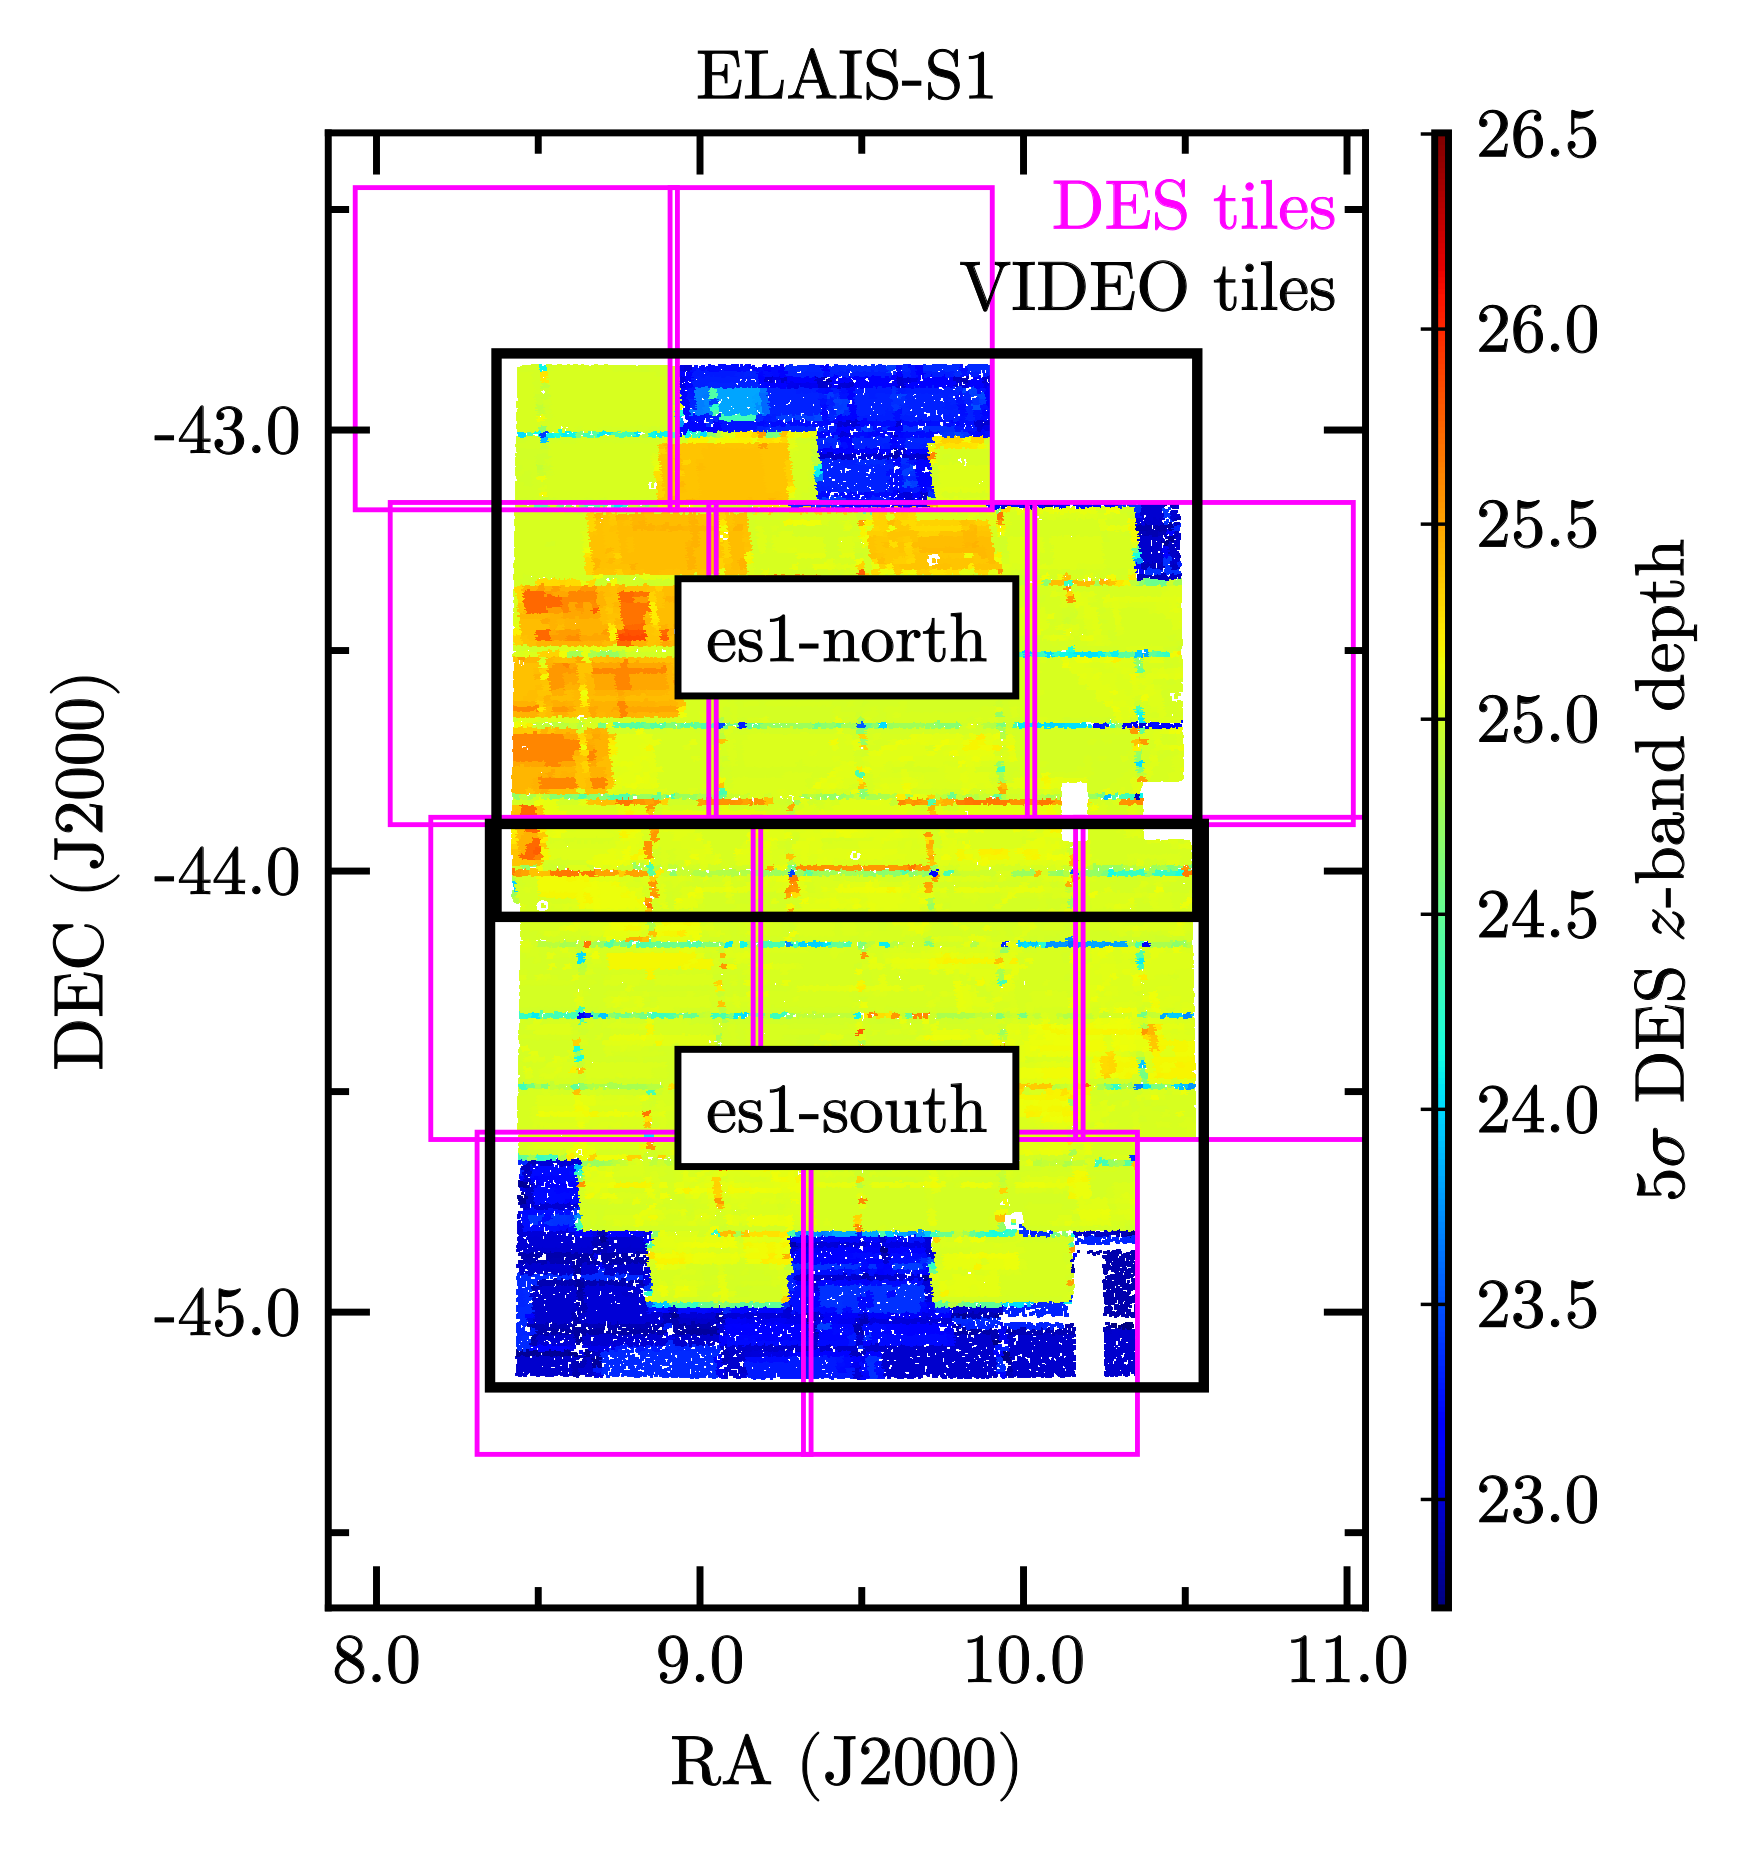
\includegraphics[width=0.618\textwidth]{field_outline_es1.png}
\caption[Depths in the ELAIS-S1 field]{$z$-band $5\sigma$ limiting magnitudes in \SI{1.95}{\arcsec} apertures for the DES data that overlaps the VIDEO footprint in the ELAIS-S1 field. These depths have been derived from the $10\sigma$ depth maps provided by the DES collaboration as detailed in the text. The DES collaboration has included the SLR corrections described in Section \ref{subsubsection:des_catalogues} in their $10\sigma$ depth estimates. The magenta squares show the edges of the DES co-add tiles. VIDEO tiles are outlined in black.}
\label{fig:depth_es1}
\end{figure}

\begin{figure}[!htb] 
\centering    
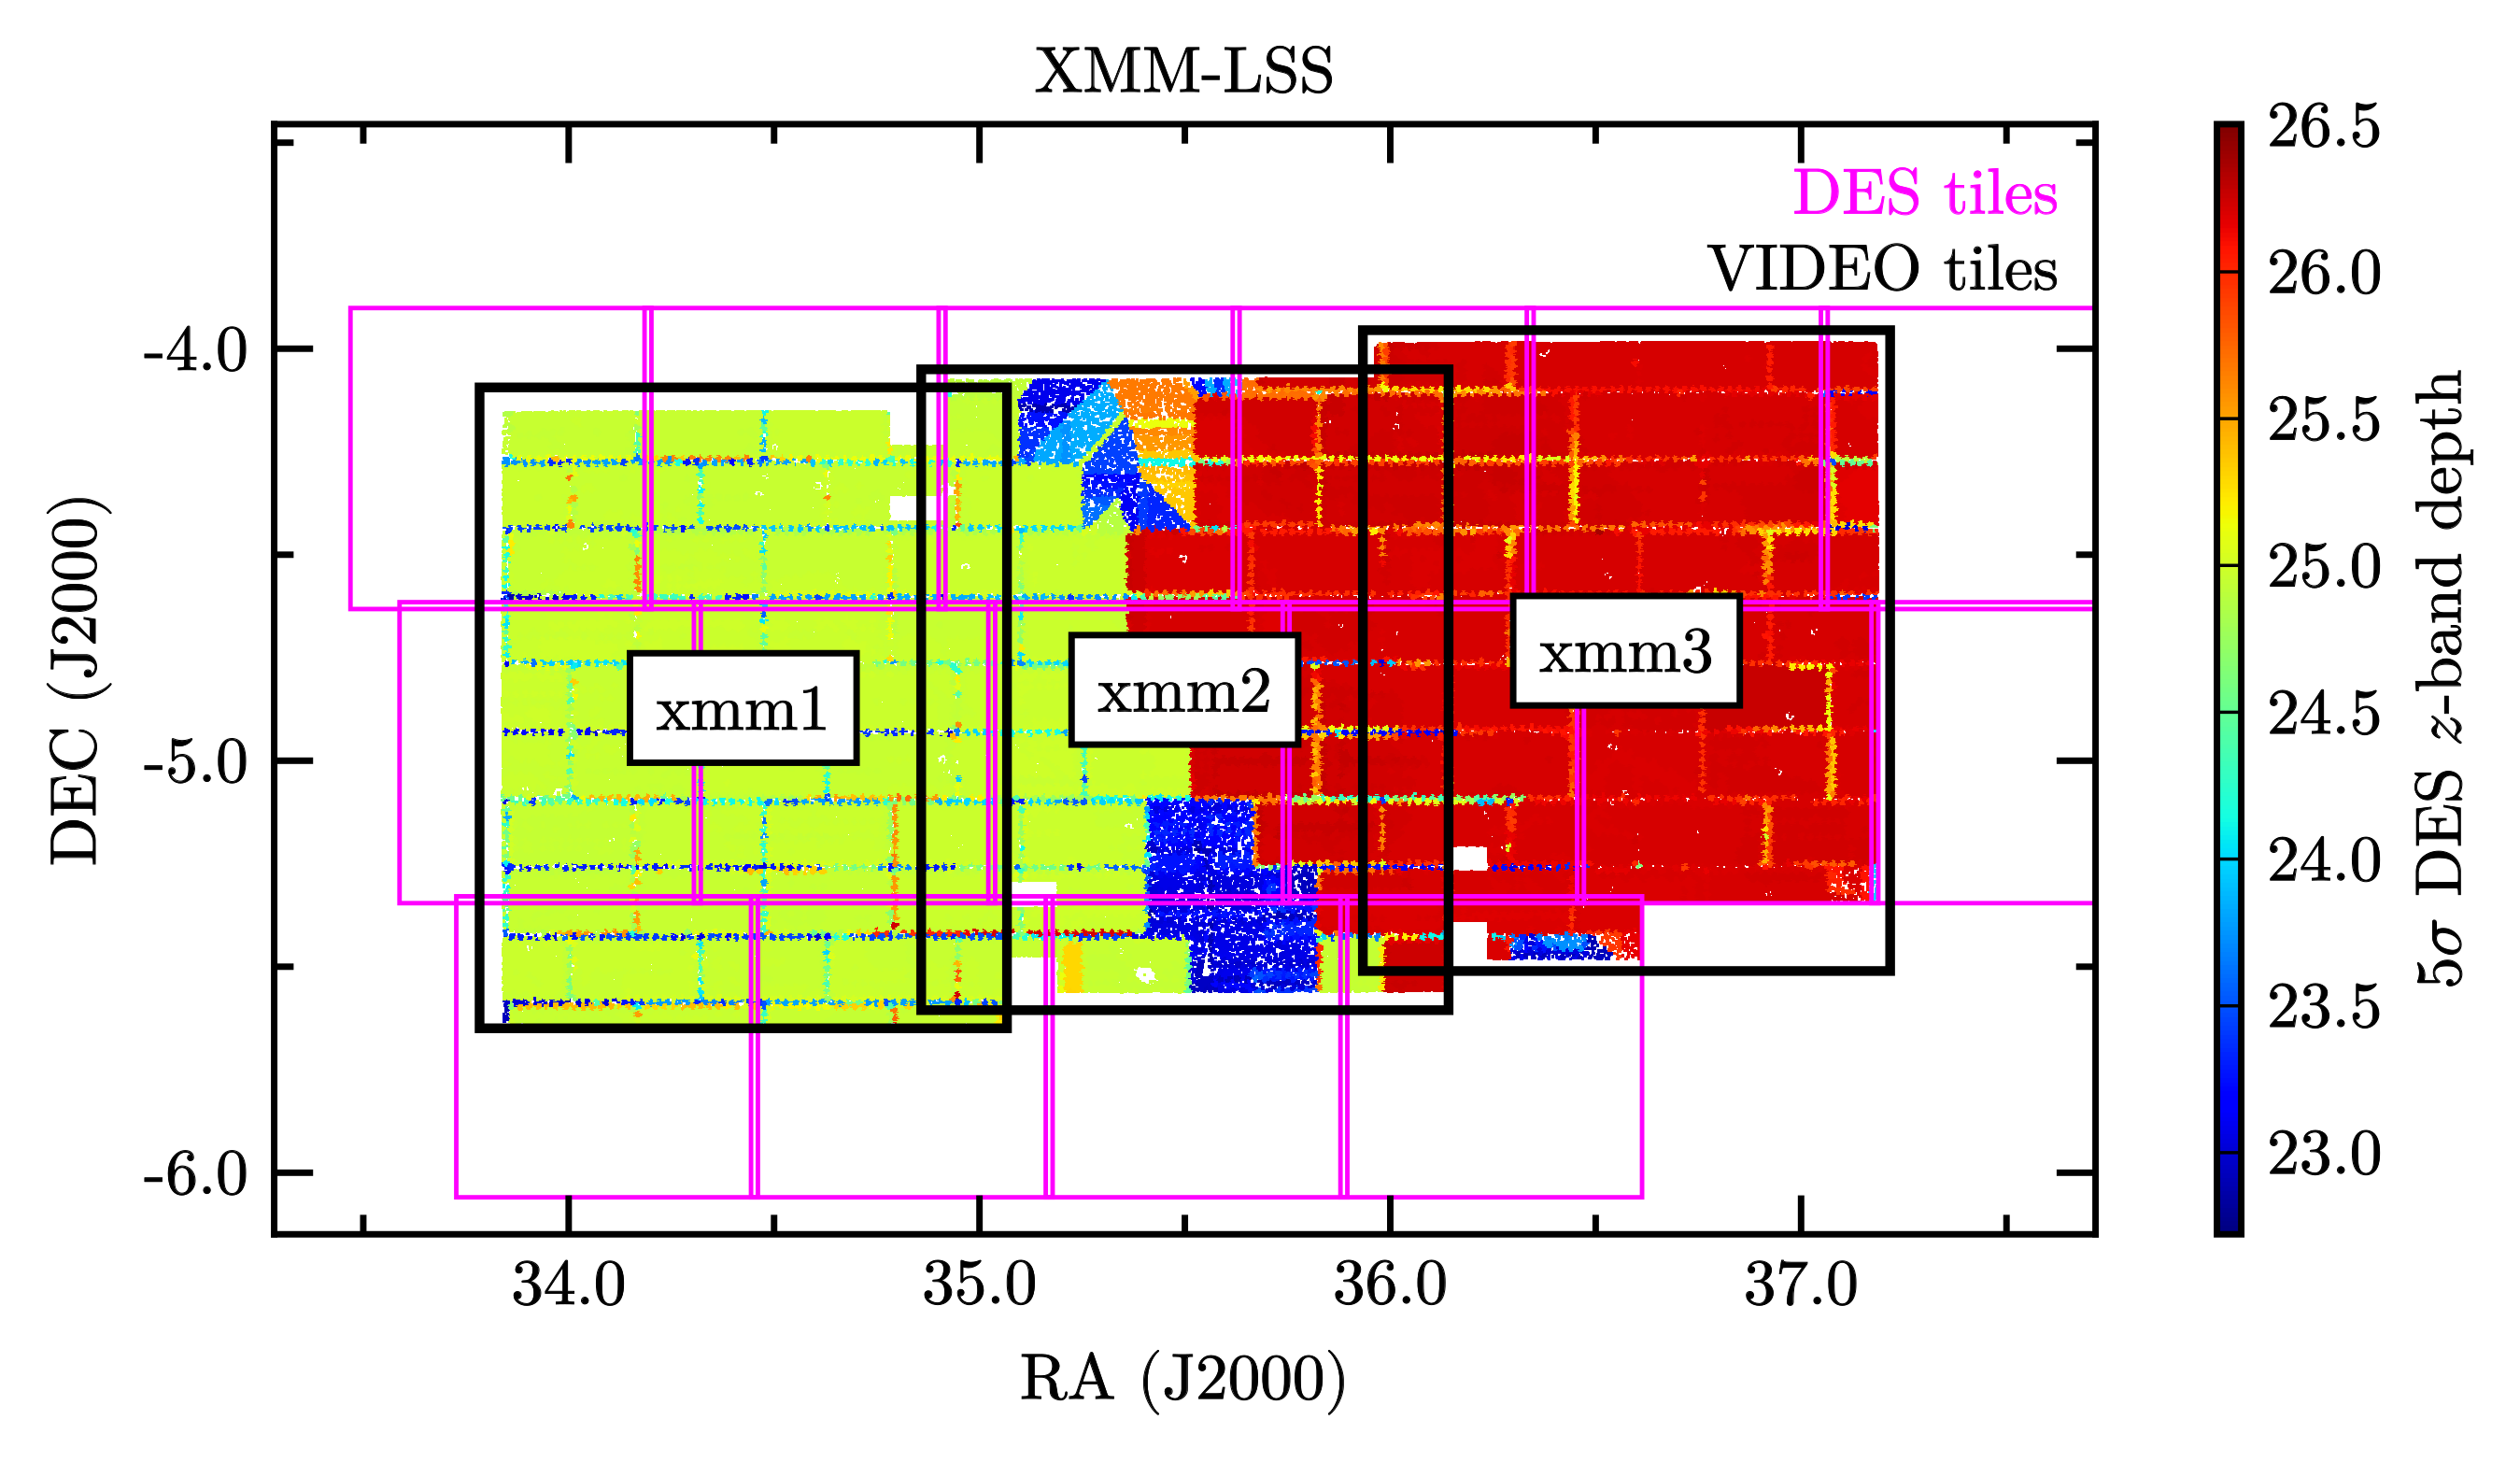
\includegraphics[width=0.95\textwidth]{field_outline_xmm.png}
\caption[Depths in the XMM-LSS field]{$z$-band $5\sigma$ limiting magnitudes in \SI{1.95}{\arcsec} apertures for the XMM-LSS field. The image description is otherwise identical to that of Figure \ref{fig:depth_es1}. The red regions correspond to the deep supernova field X3.}
\label{fig:depth_xmm}
\end{figure}

\begin{figure}[!htb] 
\centering    
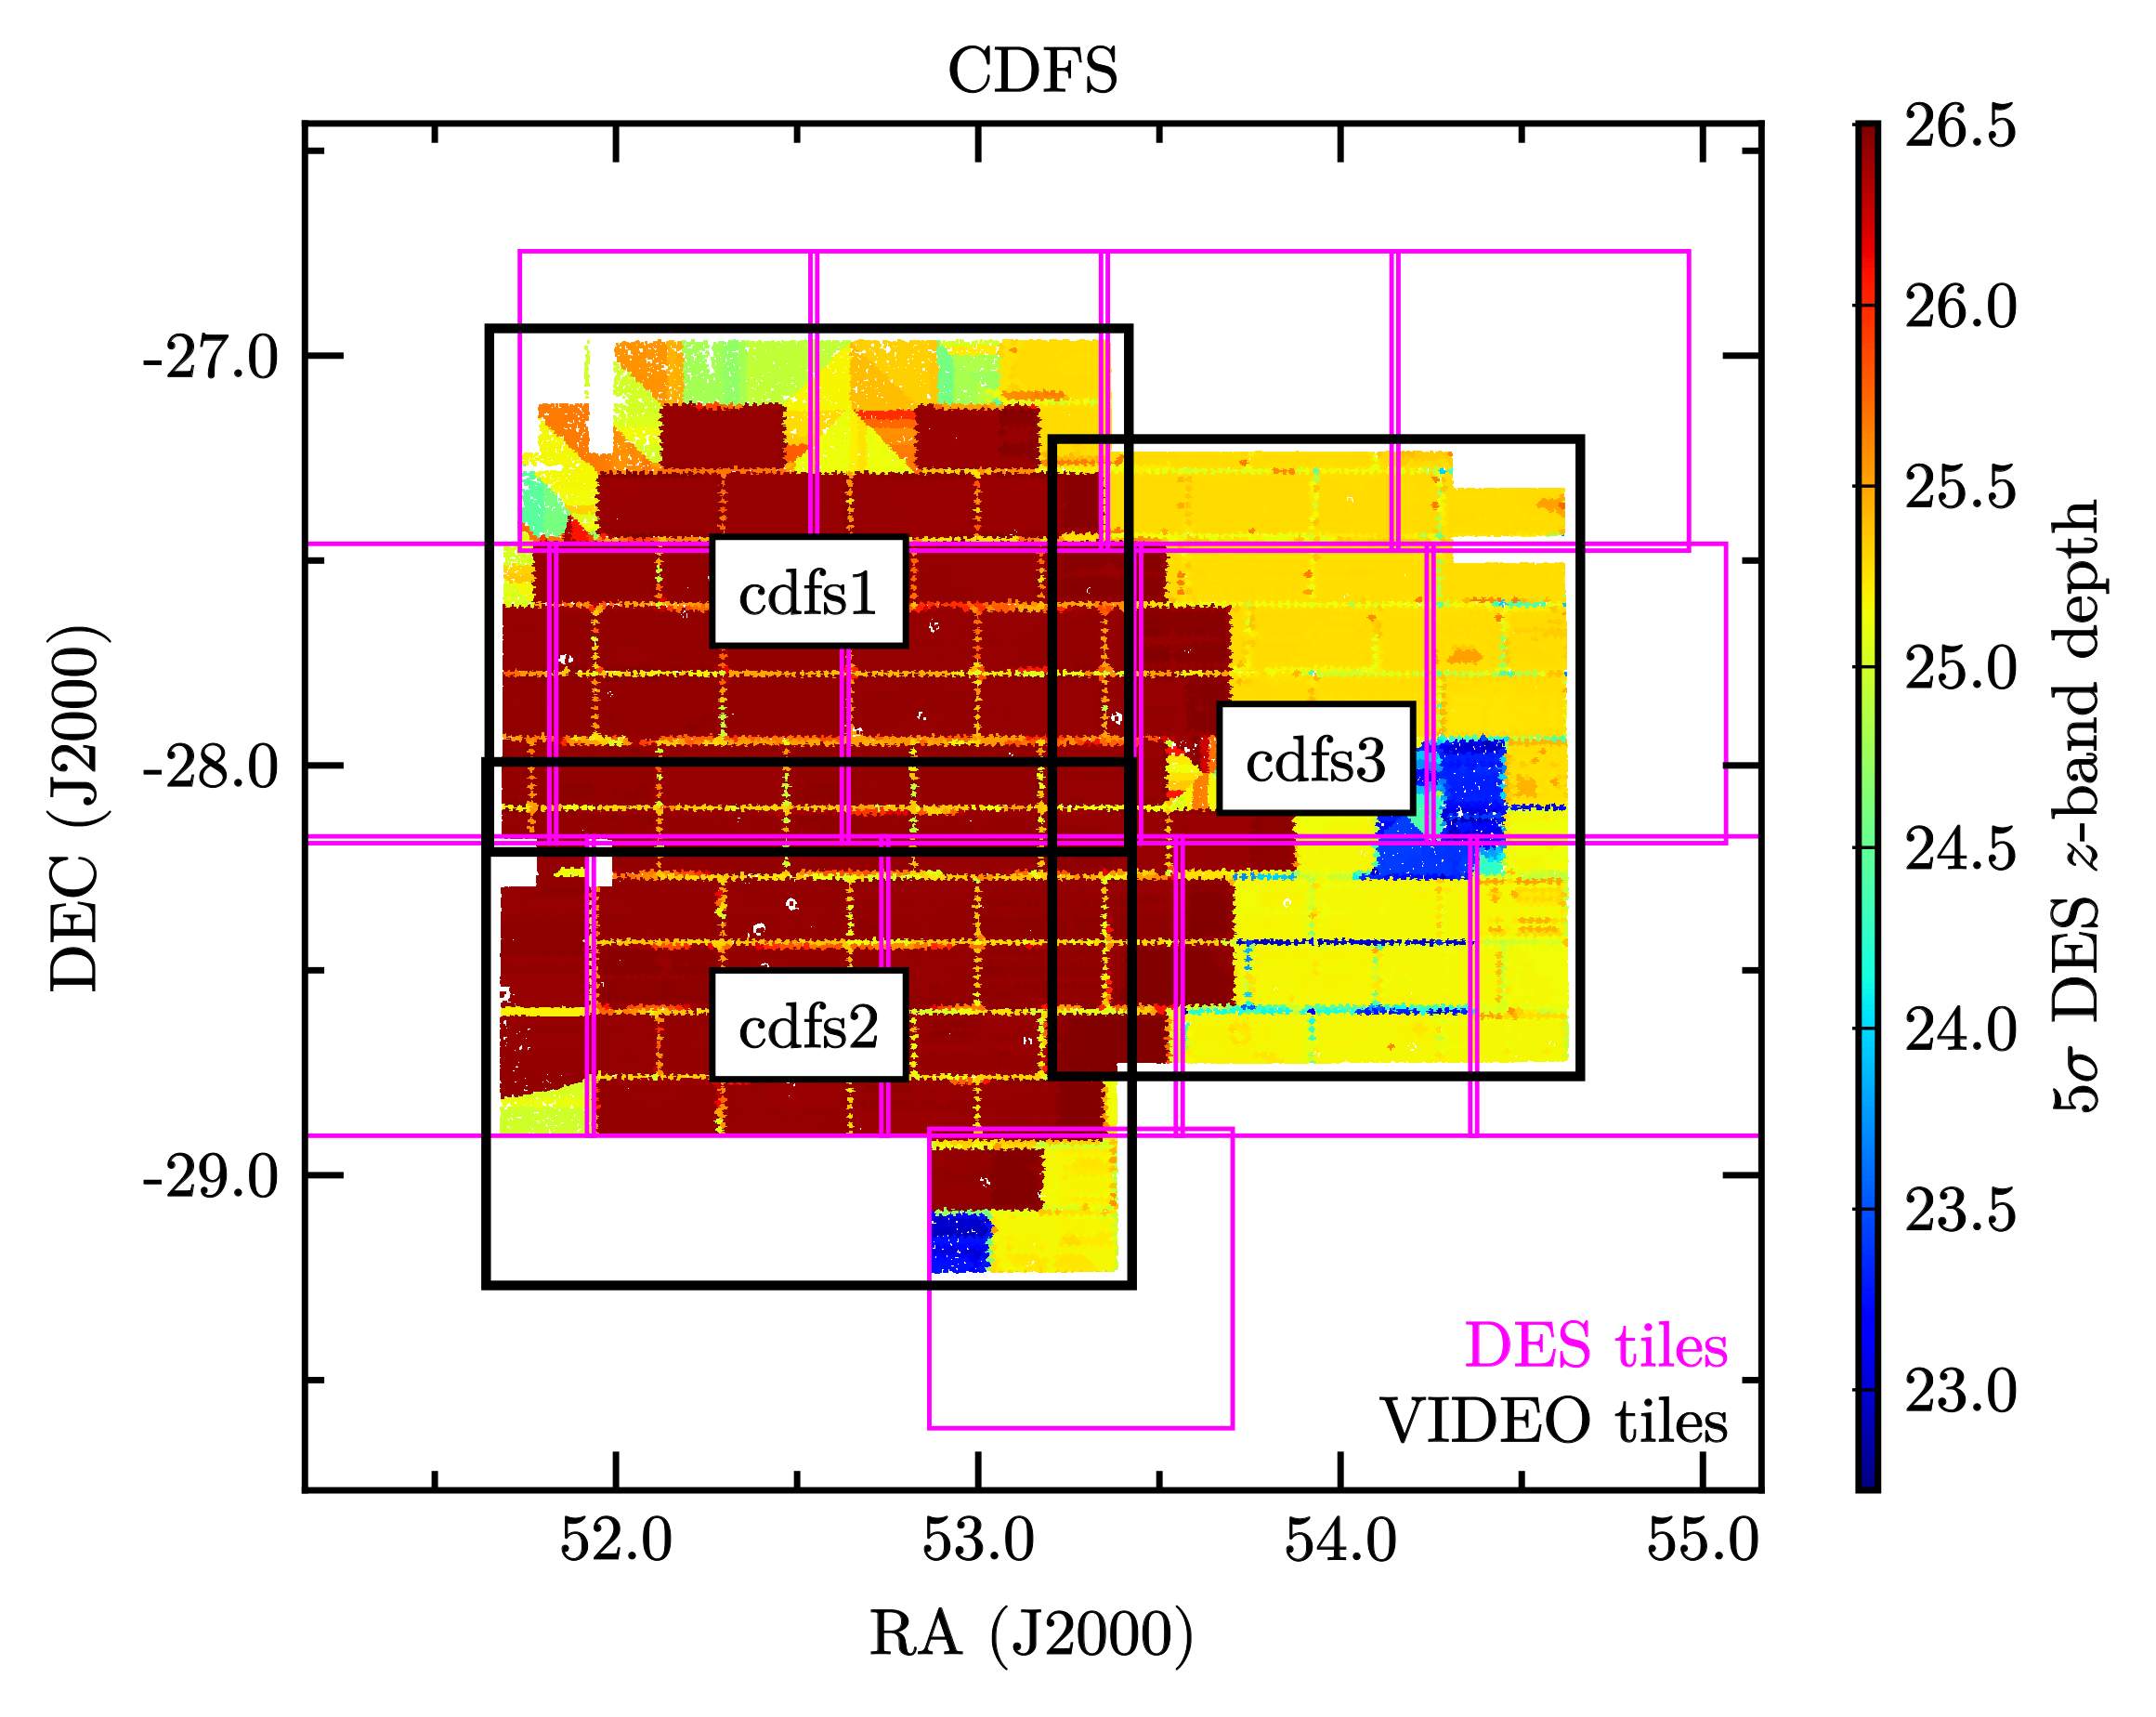
\includegraphics[width=0.825\textwidth]{field_outline_cdfs.png}
\caption[Depths in the CDF-S field]{$z$-band $5\sigma$ limiting magnitudes in \SI{1.95}{\arcsec} apertures for the CDF-S field. The image description is otherwise identical to that of Figure \ref{fig:depth_es1}. The red regions correspond to the deep supernova field C3.}
\label{fig:depth_cdfs}
\end{figure}


To visualise the depths in the eventual \DESVIDEO catalogue, the $z$-band $5\sigma$ depth maps (obtained from the $10\sigma$ DES maps as described above) are plotted in Figures \ref{fig:depth_es1}, \ref{fig:depth_xmm} and \ref{fig:depth_cdfs} for the ELAIS-S1, XMM-LSS, and CDF-S fields respectively. It must be noted that these maps contain only the DES data included in the combined \DESVIDEO catalogue, and that they thus display only regions that overlap the VIDEO survey. The plots clearly show the heterogenous nature of the DES data, as well as the imprint of the hexagonal DECam CCD array and chip gaps in between CCDs. They also illustrate the varying coverage in the DES supernova fields, clearly demonstrating the higher depths in the deepest regions X3 and C3 (see Table \ref{table:fields}). An overview of the depth variation in all DES filters is given in Table \ref{table:actual_des}, which shows the minimum, maximum and median values of the $5\sigma$ depths for the full $grizY$ filterset. \par


\begin{table}[!bt]
\centering
\textsc{$5\sigma$ limiting magnitudes in the DES deep fields} \\
\vspace{0.1em}
\footnotesize
\begin{tabular}{lcc}
\toprule\toprule
Filter & $5\sigma$ depth range (\si{\magab}) & Median $5\sigma$ depth (\si{\magab})  \\
\midrule
$g$ & 24.2 - 26.9 & 25.9 \\
$r$ & 23.8 - 26.9 & 25.6 \\
$i$ & 23.3 - 26.6 & 25.4 \\
$z$ & 22.7 - 26.5 & 25.2 \\
$Y$ & 21.2 - 23.5 & 23.1 \\
\bottomrule
\end{tabular}
\vspace{1em}
\caption[Range of depths in the DES deep fields]{Minimum, maximum, and median (averaged over area) values of the $5\sigma$ limiting magnitudes in \SI{1.95}{\arcsec} apertures, for the DES deep field data overlapping the VIDEO footprint. Values were obtained from the $5\sigma$ depth maps derived as per the text, based on the $10\sigma$ limiting magnitude maps provided by the DES collaboration. The significantly lower $Y$-band depths are explained by the fact that $Y$-band coverage is provided by the wide-area survey, which is considerably shallower. 
}
\label{table:actual_des}
\end{table}


To measure the effective area available for specific science goals, it is useful to consider the total \DESVIDEO area that is available to a given depth. This quantity is explored in Figure \ref{fig:area_depth}, which for each of the $grizY$ filters shows the relationship between a given $5\sigma$ limiting magnitude and the total area with that limiting magnitude or higher. Out of the total combined footprint of \SI{12.1}{\sqdeg}, the largest part ($\approx\SI{11}{\sqdeg}$ in $griz$) comes from the supernova fields. The remaining coverage ($\approx\SI{1}{\sqdeg}$ of the $griz$-bands and all of the $Y$-band) is from the wide-field survey. The effect of the shallow and deep supernova fields (see Table \ref{table:fields}) can be seen in the two `steps' of the $griz$ distributions. In the $z$-band, for instance, there is \SI{10.8}{\sqdeg} available to $5\sigma$ depths of $z_{5\sigma}=24.9$, originating from all eight supernova fields (deep and shallow). A sub-area of \SI{4.3}{\sqdeg} extends even further to $z_{5\sigma}=26.2$; this data comes from the deep supernova fields X3 and C3. \par

\begin{figure}[!htb] 
\centering    
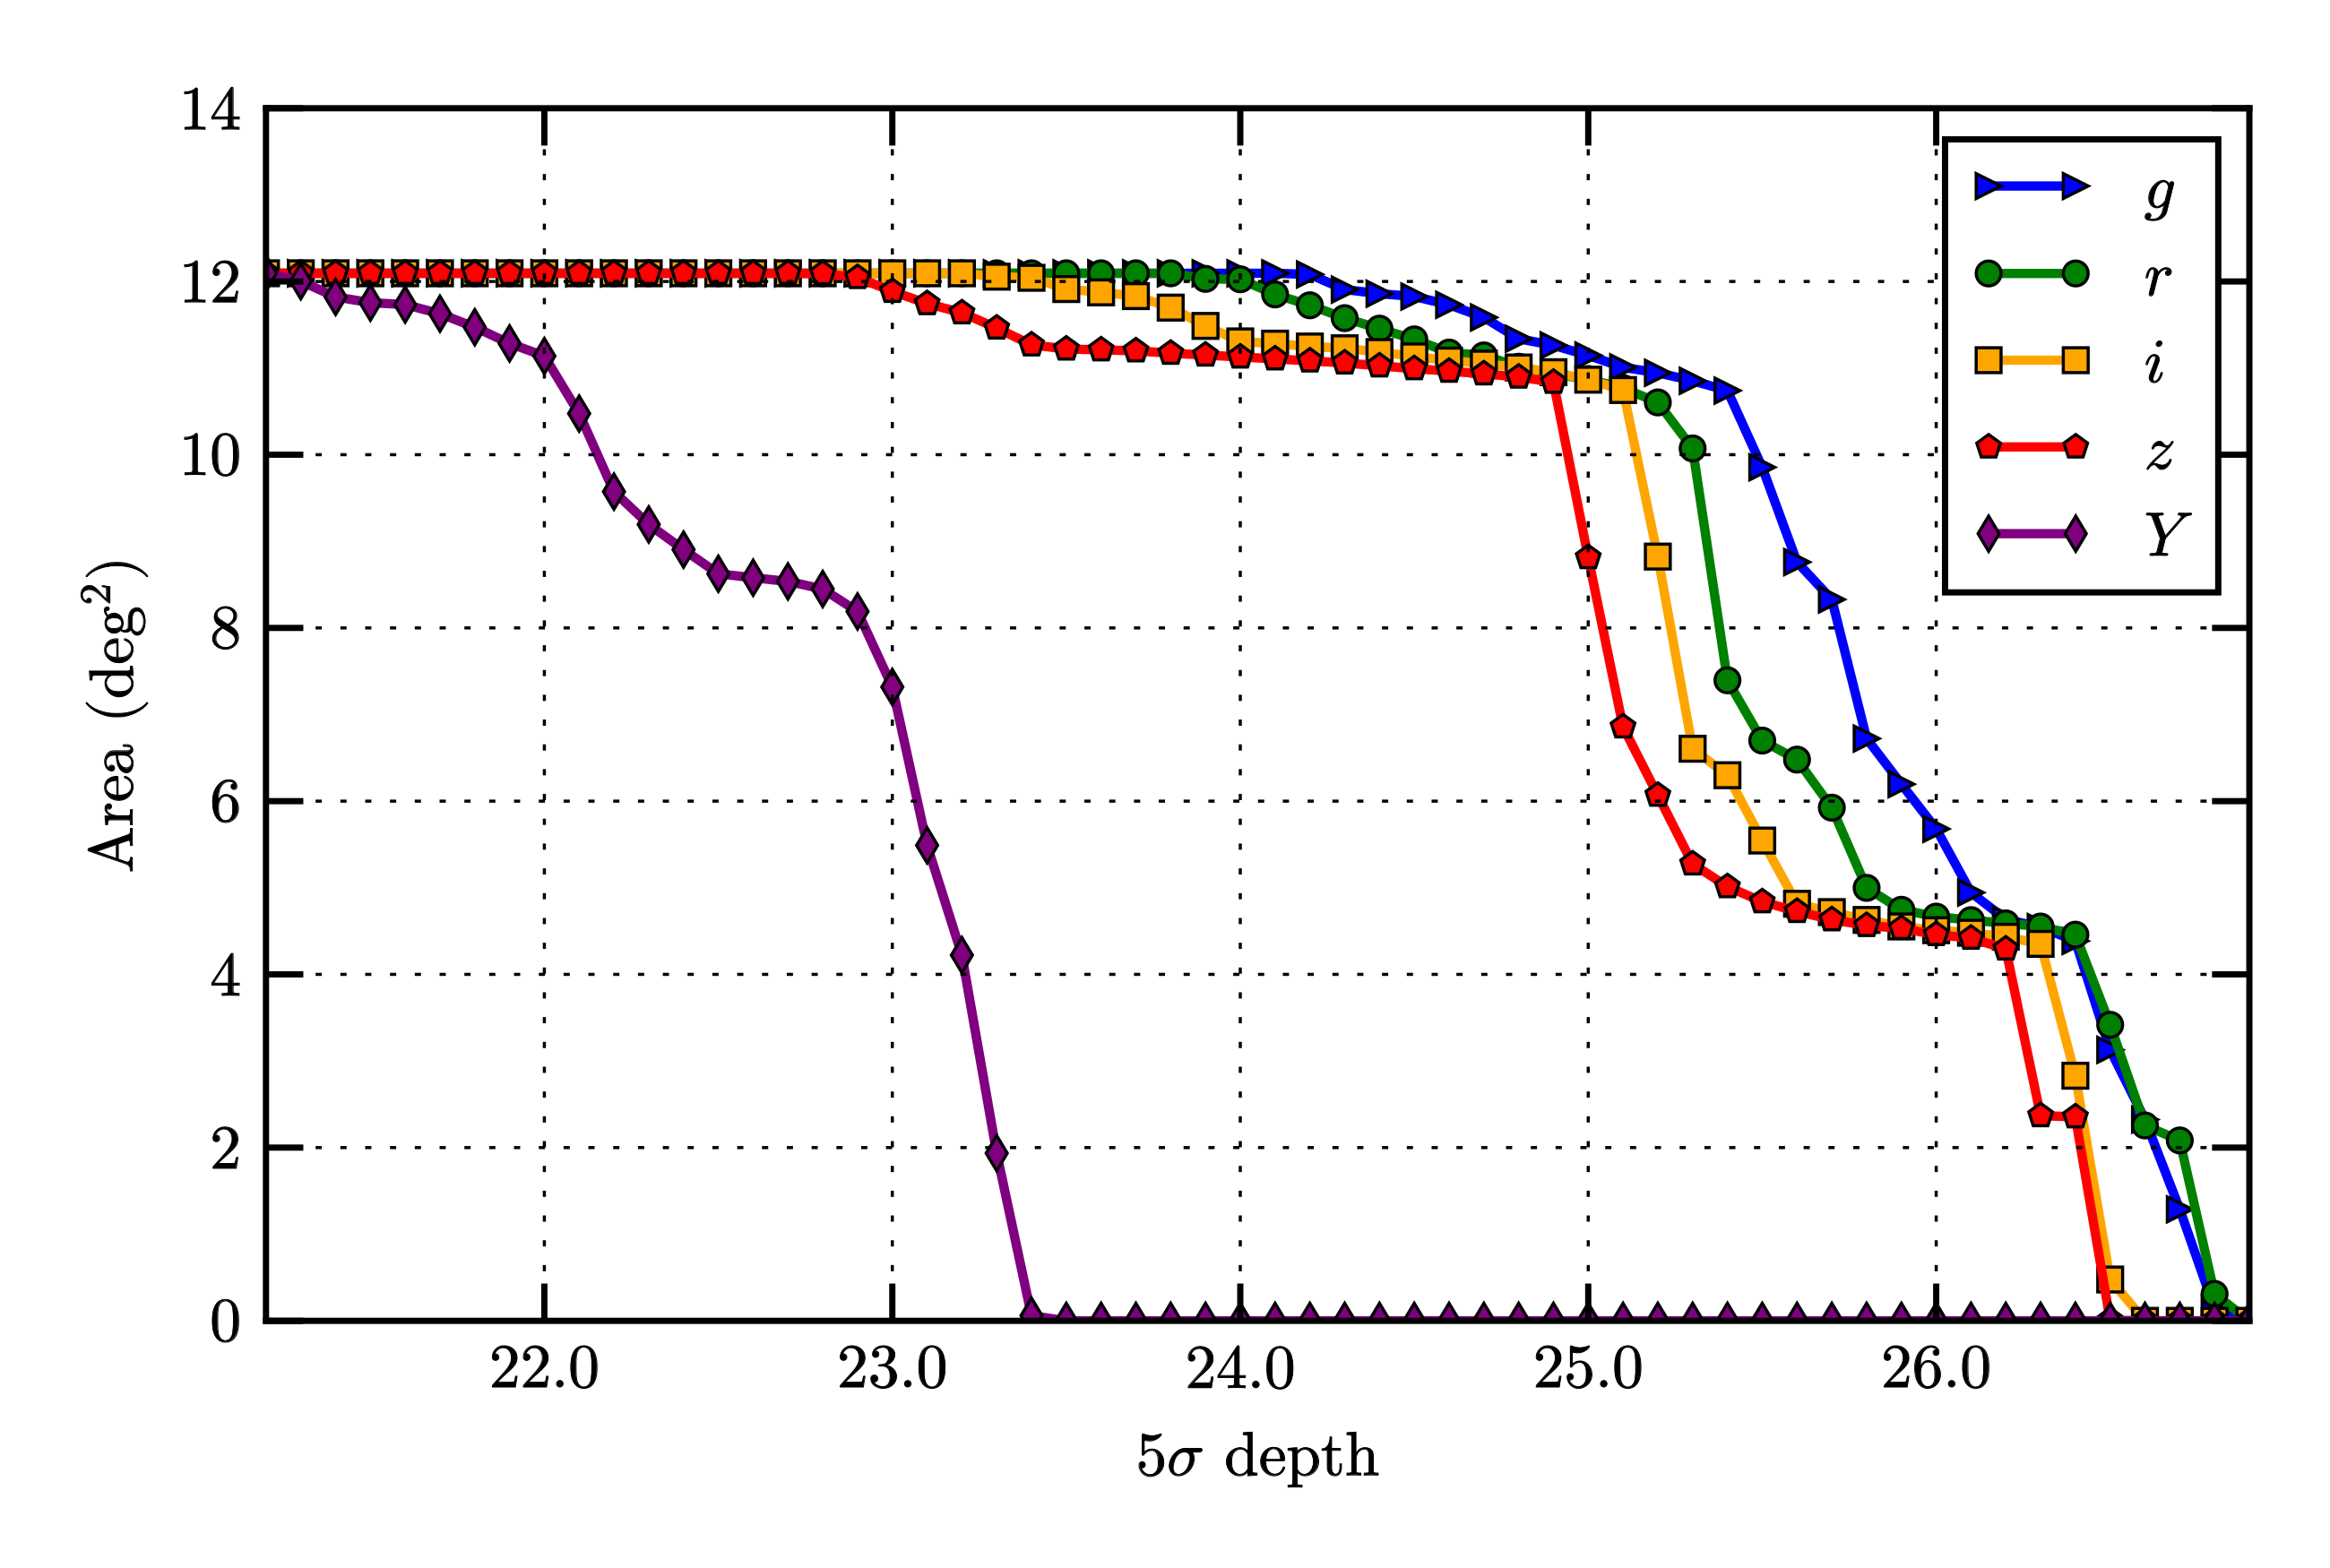
\includegraphics[width=0.95\textwidth]{area_depth_plot_5sig.png}
\caption[Area as a function of \texorpdfstring{$5\sigma$}{} depth for the total survey footprint]{The area available to a given $5\sigma$ depth as a function of that depth, for the catalogue produced in this thesis. The plotted area contains only DES data overlapping VIDEO. Area-depth functions are shown for all five DES filters.}
\label{fig:area_depth}
\end{figure}

Although the \SI{10.8}{\sqdeg} area with $z_{5\sigma}=24.9$ that remains after considering VIDEO overlap is much less than the total $\sim\SI{24}{\sqdeg}$ of DES data available, a comparison with similar surveys in Table \ref{table:ground_small_survey} demonstrates that it is still among the largest footprints to these depths. What is more, the $z_{5\sigma}=26.2$ limiting magnitudes in the deepest \SI{4.3}{\sqdeg} regions are comparable to those of the CFHTLS deep fields, which currently comprise the deepest optical imaging over $\sim \SI{4}{\sqdeg}$. The area-depth coverage of the catalogue in this thesis turns out to be even more significant when also considering the VIDEO limiting magnitudes, because together the \DESVIDEO combined footprint covers the largest area among existing optical+near-IR datasets with comparable near-infrared depths.  This point will be revisited in Section \ref{subsubsection:data_quality_video}, where the VIDEO depths will be introduced and discussed.  \par
%CHANGE THIS MAKE IT NICER 



\paragraph{Weight flags}
To identify sources with questionable photometry, the DESDM catalogues contain a \texttt{FLAGS\_WEIGHT} column that indicates when \texttt{SExtractor} extracted photometry on an object with low weights (as determined from the $r+i+z$ co-add weight maps). \texttt{SExtractor} assigns a \texttt{FLAGS\_WEIGHT} value of 1 to objects which overlap pixels in the weight map below a threshold value \texttt{WEIGHT\_THRESH}, and a value of 2 to objects that are adjacent to pixels below the \texttt{WEIGHT\_THRESH} value\footnote{More specifically, when the isophotal footprint assigned to an object by \texttt{SExtractor} overlaps or is adjacent to pixels which fall below this threshold in the detection image weight map.}. All other, unflagged sources are allocated a \texttt{FLAGS\_WEIGHT} value of 0. The DESDM pipeline used a \texttt{WEIGHT\_THRESH} threshold of 0 \citep{2018PASP..130g4501M}, which means in practice that objects with non-zero weight flags overlap or touch regions that were masked out by DESDM. As discussed in Section \ref{subsubsection:data_reduction}, these masked out regions belong to bad pixels or artefacts, for instance from faulty CCDs, chip gaps, saturated parts of bright stars, cosmic rays, and satellite or meteor trails (see \citealt{2018ApJS..235...33D} and \citealt{2018PASP..130g4501M} for the specific details of the masking algorithm). In this thesis, the weight flags are later used to filter out artefacts and objects with unreliable photometry, during the computation of \DESVIDEO photometric redshifts and the assembly of a high-redshift galaxy sample (described in Sections \ref{subsection:photoz_computation_method} and \ref{subsubsection:weight_flag_cut} respectively). \par







%********************************** %Second Section  **************************************
\subsection{The Vista Extragalactic Deep Observations Survey (VIDEO)}\label{section:video}
\subsubsection{Overview}\label{subsubsection:video_overview}
%The importance of NIR data lies in two points.
The VISTA Extragalactic Deep Observations  survey (VIDEO; \citealt{2013MNRAS.428.1281J}) is a near-infrared survey conducted with the Visible and Infrared Survey Telescope for Astronomy (VISTA). Its scientific aims are to study the evolution of galaxies, clusters, and structures as a function of their environment over the cosmic epoch $0<z<4$, and to trace AGN and the most massive galaxies out into the era of reionisation. To this end, VIDEO covers \SI{12}{\sqdeg} in five near-infrared filters ($ZYJHK_{s}$). Imaging over these wavelengths is crucial to both science goals. Firstly, near-IR data is required for the proposed $z<4$ galaxy evolution studies, because above $z>1$ the bulk of the luminosity output required for stellar mass estimates is emitted in these wavebands. Secondly, when approaching the epoch of reionisation at $z\sim6$, the light output of galaxies is almost entirely redshifted into the near-infrared. The VIDEO science goals also require deep imaging over a large area. Previous near-infrared studies have been either too shallow for high-redshift studies (e.g. VIKING, \citealt{2013Msngr.154...32E}; UKIDSS-LAS, \citealt{2007MNRAS.379.1599L}; VHS, \citealt{2013Msngr.154...35M}), or covered too small areas for statistical studies of large-scale environments and for finding uncommon objects such as massive galaxies and AGN (e.g. CANDELS, see Table \ref{table:space_small_survey}; UltraVISTA, see Table \ref{table:ground_small_survey}).  The VIDEO survey bridges this gap, utilizing the state-of-the-art rapid imaging technology on the VISTA telescope that has made it possible to efficiently probe large cosmological volumes. Its combination of area and depth makes VIDEO an ideal candidate to combine with DES optical imaging, creating a dataset excellently suited to the photometric redshift research and high-redshift galaxy search in this thesis. \par

\subsubsection{Data collection}\label{subsubsection:data_collection_video}
VIDEO observations have been conducted with the VISTA Infrared Camera (VIRCAM; \citealt{2006SPIE.6269E..0XD}) on the 4m VISTA telescope \citep{2004Msngr.117...27E, 2015A&A...575A..25S} at the La Silla Paranal observatory. VIRCAM is the world's largest near-IR camera, made up of 16 \num{2048 x 2048} HgCdTe detector arrays totalling 67 megapixel, with a mean pixel scale of \SI{0.339}{\arcsec.pix^{-1}}. The detectors are spaced out over a \SI{1.65}{deg} diameter focal plane, with gaps of 0.9 and 0.425 of a detector along the x- and y-axes respectively,  as illustrated by Figure \ref{fig:VIRCAM}. Excluding these gaps, the 16 detectors cover an effective \SI{0.6}{\sqdeg} field-of-view. The five $ZYJHK_{s}$ broadband VIRCAM filters used for VIDEO are plotted in Figure \ref{fig:filters}, with detailed wavelength coverage specified in Table \ref{table:effective_wavelengths}. \par

\begin{figure}[tbp] 
\centering    
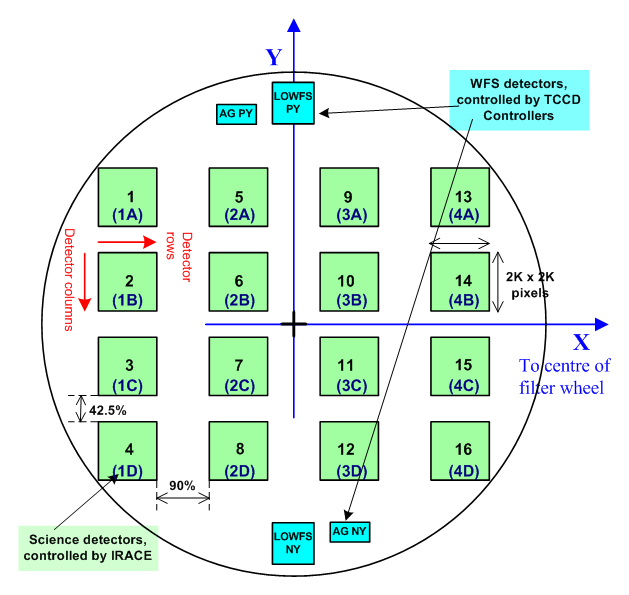
\includegraphics[width=0.75\textwidth]{VIRCAM_detail.png}
\caption[VIRCAM focal plane]{Focal plane of the VISTA Infrared Camera (VIRCAM), made up of 16 HgCdTe detectors. The detectors are spaced out with gaps of 0.9 and 0.425 of a detector in the x- and y-direction respectively. The diameter of the focal plane spans 1.65 deg, and the total effective area covered by all 16 detectors (excluding gaps) is \SI{0.6}{\sqdeg}.  \textit{Image credit:} VISTA ({\color{blue} www.vista.ac.uk})}
\label{fig:VIRCAM}
\end{figure}


Observations commenced in October 2009 and finished in September 2018. Throughout these nine years, imaging was collected using an observing strategy detailed in \cite{2013MNRAS.428.1281J}, which will be now be summarised  briefly. The VIDEO protocol was designed to deal with well-known challenges for near-infrared astronomy, concerning the brightness and variability of the sky background in this wavelength regime (particularly in the $H$- and $K_{s}$-bands). To overcome these issues, individual exposures were split up into small time chunks. Each pointing was observed NDIT times, with a detector integration time DIT (between 10 and 50 seconds depending on the filter), resulting in a total exposure time of $\mathrm{NDIT} \times \mathrm{DIT}$. The telescope was then `jittered' randomly by a small offset of $\lesssim\SI{20}{\arcsec}$, and the $\mathrm{NDIT} \times \mathrm{DIT}$ sequence was repeated at the offset position. This jittering minimises the effect of  both sky fluctuations and detector artefacts such as bad pixels. The totality of $\mathrm{NDIT} \times \mathrm{DIT}$ (jittered) exposures in a given position is called a `paw-print' in VIDEO jargon. Due to the aforementioned gaps between VIRCAM  detectors, these paw-prints do not fill a contiguous area. To cover a full tile, the telescope was moved in a sequence of six offsets in the x- and y-direction, with paw-prints taken in each of these positions. When added together, they produce a VIDEO tile with a total area of $\sim 1 \times \SI{1.5}{\sqdeg}$. \par 



\begin{table}[htb]
\centering
\textsc{VIDEO fields} \\
\vspace{0.1em}
\footnotesize
\begin{tabular}{llccc}
\toprule\toprule
VIDEO name & Field  & R.A. (J2000) & DEC (J2000) & Available filters  \\
\midrule
es1-north & ELAIS-S1 & 00:37:49 & -43:29:53 & $ZYJHK_{s}$\\
es1-south & ELAIS-S1 & 00:37:49 & -44:29:53 & $ZYJHK_{s}$ \\
xmm1 & XMM-LSS & 02:17:42 & -04:51:00 & $ZYHK_{s}$ \\
xmm2 & XMM-LSS & 02:22:00 & -04:48:00 & $YJHK_{s}$ \\
xmm3 & XMM-LSS & 02:26:18 & -04:44:00 & $ZYJHK_{s}$ \\
cdfs1 & CDF-S & 03:30:08 & -27:34:30 & $ZYJHK_{s}$ \\
cdfs2 & CDF-S & 03:30:08 & -28:38:00 & $JHK_{s}$\\
cdfs3 & CDF-S & 03:34:44 & -27:59:00 & $JK_{s}$ \\
\bottomrule
\end{tabular}
\vspace{1em}
\caption[Coordinates of the VIDEO tiles]{Central coordinates for all eight $\sim \SI{1 x 1.5}{\sqdeg}$ VIDEO tiles. The positioning of these tiles, as well as the overlap with DES data, is shown in Figures \ref{fig:depth_es1}, \ref{fig:depth_xmm} and \ref{fig:depth_cdfs} for the ELAIS-S1, XMM-LSS and CDF-S respectively. The filters listed under `available filters' are all the VIDEO wavebands that were observed in the DR5 data release used in this thesis. The number of filters differs across tiles, because the survey had not yet been completed in this release.}
\label{table:VIDEO_fields}
\end{table}

 
The VIDEO survey targeted three fields, which mostly overlap with the DES deep fields introduced in Section \ref{subsubsection:data_collection} and Table \ref{table:fields}. The ELAIS-S1 field contains two VIDEO tiles extending over \SI{3}{\sqdeg}, and the XMM-LSS and CDF-S fields each encompass three VIDEO tiles totalling \SI{4.5}{\sqdeg} for each field. These eight tiles make up the total $\sim \SI{12}{\sqdeg}$ VIDEO footprint. The central coordinates of the VIDEO tiles are given in Table \ref{table:VIDEO_fields}, and their placement is mapped out in Figures \ref{fig:depth_es1}, \ref{fig:depth_xmm} and \ref{fig:depth_cdfs}, which also illustrate the intersection with the DES data.  As mentioned previously in Section \ref{subsubsection:data_quality}, the total overlap area comprises \SI{12.1}{\sqdeg}, with \SI{10.8}{\sqdeg} covered by deep field DES observations with limiting magnitudes $z_{5\sigma}\geq24.9$. \par 

This thesis uses imaging from the fifth VIDEO data release (DR5), which is the most recent publicly available dataset at the Edinburgh VISTA Science Archive\footnote{\color{blue} http://horus.roe.ac.uk/vsa/}. This dataset includes observations taken up to 25 March 2015, and is identified by the date stamp \texttt{2015-03-25} internally to the VIDEO collaboration. As the survey was not yet completed at this time, some tiles in this release do not contain observations in every filter. Table \ref{table:VIDEO_fields} lists the filters that are available in each tile. Some tiles and filters have also progressed further than others in terms of exposure times, resulting in some depth variation between tiles. The extent of this variation will be presented in Section \ref{subsubsection:data_quality_video}. Regarding future data releases, it is useful to mention once more that the \DESVIDEO catalogue production pipeline created in this thesis is largely automated, so that it will be straightforward to include future VIDEO data. \par

\subsubsection{Data reduction}\label{subsubsection:video_data_reduction}
Data reduction for the VIDEO survey was performed by the Cambridge Astronomical Survey Unit (CASU) and \cite{2013MNRAS.428.1281J}. A summary of the procedure is provided below, and the reader is referred to \cite{2013MNRAS.428.1281J} for the full details. The initial data processing steps were conducted by CASU using a pipeline specially developed for VIRCAM data, detailed in \cite{2004SPIE.5493..411I} and updated on the CASU website\footnote{\color{blue} http://casu.ast.cam.ac.uk/surveys-projects/vista/technical/data-processing}. The CASU system firstly processed each $\mathrm{NDIT} \times \mathrm{DIT}$ raw data frame, removing instrument signatures, performing photometric calibration, applying sky background subtraction\footnote{The background correction for VIDEO differs from the default CASU pipeline. As explained in \cite{2013MNRAS.428.1281J}, the VIDEO depths require a special fine-tuned sky subtraction procedure.}, and producing confidence (i.e. weight) maps. CASU then created paw-prints by stacking all jittered iterations of the processed raw data frames, applying outlier rejection to artefacts such as bad pixels, cosmic rays, and fast-moving transients. Stacked weight maps for each paw-print were created at the same time. Afterwards, \cite{2013MNRAS.428.1281J} combined these paw-prints into co-added tiles and co-added weight maps, using \texttt{SWarp} to stack images via a weighted mean algorithm. Paw-prints with a seeing worse than $\mathrm{FWHM}<\SI{0.9}{\arcsec}$ were rejected before co-addition. During the co-addition process, all images were resampled to a pixel scale of \SI{0.2}{\arcsec.pix^{-1}}. The resulting VIDEO images and weight maps make up the imaging from which the near-infrared photometry for this thesis is extracted. \par 



\paragraph{Catalogues}
\cite{2013MNRAS.428.1281J} also produced VIDEO catalogues from the co-add images, assembled via several iterations of \texttt{SExtractor}. In each run, \cite{2013MNRAS.428.1281J} used dual-image mode to extract photometry in a given band, with detection performed in a different band for each iteration (see Section \ref{subsubsection:forced_phot_extraction} for an illustrative application of double-image mode). As an example, they created four catalogues for the $Z$-band, each of which was based on detections in one of the $Y$, $J$, $H$ or $K_{s}$ filters. They then merged these \texttt{SExtractor} iterations into a final catalogue for each tile, retaining only the longest wavelength detection for sources detected in multiple bands. Lastly, \cite{2013MNRAS.428.1281J} corrected their photometric errors in order to account for correlated noise. More detail on all these catalogues can be found in \cite{2013MNRAS.428.1281J}. \par 

It is emphasised that this thesis does not make use of the \cite{2013MNRAS.428.1281J} photometry for the \DESVIDEO catalogue. Instead, VIDEO fluxes in this thesis are extracted straight from the VIDEO co-adds via a forced photometry method that will be introduced in Section \ref{section:forced_photometry}. The \cite{2013MNRAS.428.1281J} catalogues\footnote{Throughout this thesis, these datasets will be referred to as the \cite{2013MNRAS.428.1281J} catalogues, although the version used in this thesis is an updated version from the DR5 data release based on data up to 2015.} are briefly used afterwards to verify the forced photometry results. In this way, they do play a role in assessing the validity of the \DESVIDEO catalogue. \par 



\subsubsection{Data quality}\label{subsubsection:data_quality_video}
It is useful to examine the quality of the VIDEO imaging. Just like the DES quality assessment in Section \ref{subsubsection:data_quality}, this analysis will once again focus on the seeing, depths, and weight flags. \par


\paragraph{Seeing} The VIDEO observing protocol required that observations be carried out in good seeing --- for each filter it was required that $\mathrm{FWHM} < \SI{0.8}{\arcsec}$. However, because observing conditions could change over an observation period, exposures with seeing up to $\mathrm{FWHM} < \SI{0.9}{\arcsec}$ were also included in the co-add tiles. Over the total survey, the mean seeing is \SIlist[list-units = brackets]{0.84; 0.81; 0.79; 0.78; 0.78}{\arcsec} for the $Z$, $Y$, $J$, $H$, and $K_{s}$ filters respectively\footnote{These values were derived by the author based on VIDEO collaboration measurements of the average seeing in each VIDEO tile. The mean was then obtained by averaging these tiles.}.  The smallest seeing of \SI{0.72}{\arcsec} was achieved in the cdfs2 $H$-band, and the largest value of \SI{0.85}{\arcsec} in the cdfs1 $Z$-band.  \par


\paragraph{Depths} The VIDEO observing strategy detailed in Section \ref{subsubsection:data_collection_video} produced reasonably uniform coverage inside each tile. Unlike the DES imaging, the VIDEO tiles do not contain any chip gaps. Nevertheless, some sections in the tiles are slightly deeper than average. These regions are made up of an above average number of exposures, as a result of detector overlap between paw-print shifts. At the same time, some other areas contain below average depths. This is particularly the case in regions with poor detector performance, as well as in two $\sim \SI{0.1}{deg}$ strips at the edges which have only been sampled once (by a single paw-print). The depth variation that results from all these effects is captured by the co-add weight maps. An example weight map for the $K_{s}$-band in the xmm3 tile is shown in Figure \ref{fig:weight_map}.  \par


\begin{figure}[!tb] 
\centering    
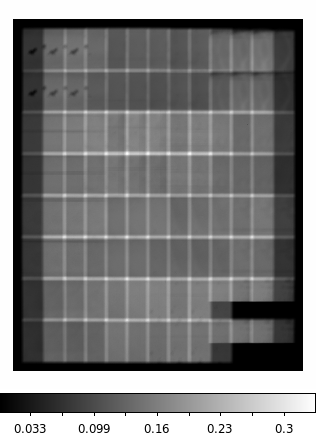
\includegraphics[width=0.5\textwidth]{Chapter2/Figs/xmm3_Ks_weights.png}
\caption[Example weight map]{Weight map for the $K_{s}$-band in the xmm3 tile. Weight values are displayed on a linear scale indicated by the bar. The two black regions in the bottom right corner are due to time-varying quantum efficiency in detector 16. Because flat fielding in that detector is extremely challenging, data from those regions has been assigned zero weight. In the top right a small region has lower weights due to dead pixels in detector 1.}
\label{fig:weight_map}
\end{figure}




In spite of the small divergent regions described above and in the caption to Figure \ref{fig:weight_map}, the overall coverage within a VIDEO tile is fairly uniform. However, even though the tiles themselves are much more uniform than the DES imaging, the VIDEO survey still contains some depth variation between tiles. This is due to the fact that the survey was not yet completed for the data release used in this thesis, so not all tiles had yet been allocated the same exposure time. To explore the variation of VIDEO depths in the \DESVIDEO catalogue, the author computed the $5\sigma$ limiting magnitudes in a \SI{1.95}{\arcsec} aperture for each tile. The procedure for calculating these values is as follows. Firstly, the $5\sigma$ limiting fluxes $F_{5\sigma}$ are derived. Because $F_{5\sigma}$ is simply defined as the flux for which the signal-to-noise ratio (S/N) equals 5, the following equation holds:


\begin{equation}
\mathrm{S/N} \equiv \frac{F_{5\sigma}}{F_{\mathrm{error}}} = 5,\label{eqn:video_signal_noise}
\end{equation}

\noindent where $F_{\mathrm{error}}$ is the VIDEO flux error in a \SI{1.95}{\arcsec} aperture. It follows that $F_{\mathrm{error}}$ can therefore be used to obtain the corresponding limiting flux $F_{5\sigma}$. Section \ref{subsubsection:error_discussion} will describe the way those uncertainties are computed for the \DESVIDEO catalogue in this thesis. The method involves an approximation whereby flux errors in a given aperture are assigned a constant value throughout each VIDEO tile. Because this approximation entails that $F_{\mathrm{error}}$ is constant, for each tile the limiting fluxes can be computed via a single instance of Equation \ref{eqn:video_signal_noise}. The limiting fluxes are then converted into magnitudes to obtain the  the final depths in each tile: 


\begin{equation}
m_{5\sigma} = m_{\mathrm{zp}} - 2.5\log{F_{5\sigma}} = m_{\mathrm{zp}} - 2.5 \log{\left( 5F_{\mathrm{error}} \right)},\label{eqn:m_n_video}
\end{equation}

\noindent where $m_{\mathrm{zp}}=-48.6$ is the AB zero-point. Table \ref{table:VIDEO_depths} shows the range in VIDEO depths derived in this way, listing the magnitude in the shallowest and deepest tiles for each filter. \par 


\begin{table}[!htb]
\centering
\textsc{VIDEO $5\sigma$ limiting magnitudes} \\
\vspace{0.1em}
\footnotesize
\begin{tabular}{lc}
\toprule\toprule
Filter &  $5\sigma$ Depth (\si{\magab}) \\
\midrule
$Z$ & 24.8 - 25.3 \\
$Y$ & 24.6 - 24.9 \\
$J$ & 23.9 - 24.6 \\
$H$ & 23.3 - 24.1 \\
$K_{s}$ & 22.9 - 23.8 \\
\bottomrule
\end{tabular}
\vspace{1em}
\caption[Minimum and maximum depths in the VIDEO data]{Minimum and maximum VIDEO $5\sigma$ depths in a \SI{1.95}{\arcsec} aperture in the \DESVIDEO catalogue. These limiting magnitudes were estimated from the catalogue photometric errors as described in the text. Depths were approximated to be constant across tiles, and the range of depths observed originates from variation between tiles. Depth variation occurs because in the data release used in this thesis the full survey depth has not been achieved in all tiles. }
\label{table:VIDEO_depths}
\end{table}

\paragraph{Weight flags} Weight flags for the VIDEO portion of the \DESVIDEO catalogue are produced by \texttt{SExtractor} during the extraction of forced photometry (see Section \ref{subsubsection:forced_phot_extraction}). As with the DESDM catalogues, non-zero weight flags identify objects that contain or touch pixels with zero weight in the co-add weight maps. For the VIDEO data, these are pixels at the very edge of the imaging and in the regions covered by detector 16 (see the bottom right of Figure \ref{fig:weight_map}). In the same way as for DES, this thesis uses the VIDEO weight flags to filter out artefacts and objects with unreliable photometry, during the computation of photometric redshift and the selection of high-redshift galaxies (see Sections \ref{subsection:photoz_computation_method} and \ref{subsubsection:weight_flag_cut} respectively).  \par


\subsection{Spectroscopic redshifts}\label{subsection:spectra}
To complement the broadband imaging and catalogues, the DES collaboration has compiled a master spectroscopic catalogue of publicly available galaxy spectra that overlap the DES footprint, published in the DES Science Portal database\footnote{\color{blue} http://cdcvs.fnal.gov/redmine/projects/des/wiki/SciencePortalProducts} \citep{2018A&C....24...52F}. This thesis uses the final \texttt{Y1A1} version (from 25 January 2016), with DESDM table name \texttt{brportal.e\_10022146\_295159}.  \par

%I GOT UP TO HERE
The master catalogue includes \num{759 535} galaxy spectra from 31 public surveys in the literature, and contains good quality flags for all objects. However, a quick investigation of the spectra revealed that some galaxies from the EBOSS survey\footnote{The source name for this survey is  \texttt{DES\_EBOSS\_ELG} in the master catalogue.} have unreliable redshifts. These objects have been assigned spectroscopic redshifts of $z_{\mathrm{spec}}>3.0$, while the DES imaging clearly indicates that they are bright ($z_{\mathrm{AB}}\lesssim20$) resolved galaxies, implying they cannot be at such high redshifts. For this reason, it was decided to remove all 335 EBOSS objects with $z_{\mathrm{spec}}>3.0$ from the master catalogue, so that \num{759 200} galaxies remain. These objects are later matched to the \DESVIDEO sources by position (within a \SI{1}{\arcsec} radius), via a process described in Section \ref{subsection:photoz_computation_method}. This matching strategy also removes any spectra with bad \texttt{FLAGS\_WEIGHT} values in any \DESVIDEO filter. At the end, these steps produced a final sample of \num{35596} galaxy spectra with \DESVIDEO photometry. The 21 spectroscopic surveys from which these spectra have been sourced are listed in Table \ref{table:spectra}, together with the fractional contribution of each survey to the total number of \DESVIDEO spectroscopic redshifts. \par 


\begin{table}[!htb]
\centering
\textsc{Sources of spectroscopic redshifts} \\
\vspace{0.1em}
\footnotesize
\begin{tabular}{lclc}
\toprule\toprule
Survey  & \% of total redshifts & Survey & \% of total redshifts \\
\midrule
3DHST & 18.9 \% & SNLS\_FORS & 1.3 \% \\
DES\_AAOMEGA & 16.5 \% & SPARCS & 0.8 \% \\
VVDS & 12.8 \% & VUDS & 0.3 \% \\
ACES & 11.9 \% & 2DF & 0.3 \% \\
GAMA & 9.6 \% & SNLS\_AAO & 0.3 \% \\
EBOSS\_DES\_ELG & 9.2 \% &  STALIN & 0.2 \% \\
NOAO\_OZDES & 8.5 \% & CDB & 0.2 \% \\
UDS & 3.5 \% & 6DF & < 0.1 \% \\
PANSTARRS & 2.4 \% & MOSFIRE & < 0.1 \% \\
ATLAS & 1.6 \% & LCRS & < 0.1 \% \\
SDSS\_OZDES & 1.5 \% & & \\

\bottomrule
\end{tabular}
\vspace{1em}
\caption[Spectra and source surveys]{Publicly available spectroscopic redshift surveys that make up the spectra in the \DESVIDEO catalogue. Spectra have been sourced from the final \texttt{Y1A1} catalogue described in the text. The names in the `Survey' column correspond to the \texttt{SOURCE} tag in this table.}
\label{table:spectra}
\end{table}

Figure \ref{fig:spectra} shows the redshift distribution of the \DESVIDEO spectra, for both the entire dataset and the ELAIS-S1, XMM-LSS, and CDF-S fields individually. With regard to the high-redshift galaxy search later in this thesis, it is important to note that the vast majority of spectra are concentrated at $z_{\mathrm{spec}}<1.0$, with only 11 at $z_{\mathrm{spec}}>4.0$ and none at $z_{\mathrm{spec}}>5.0$. The absence of available spectra at high redshifts impacts the photometric redshift strategy in Chapter \ref{chapter:photometric_redshifts}. \par 


\begin{figure}[!htb] 
\centering    
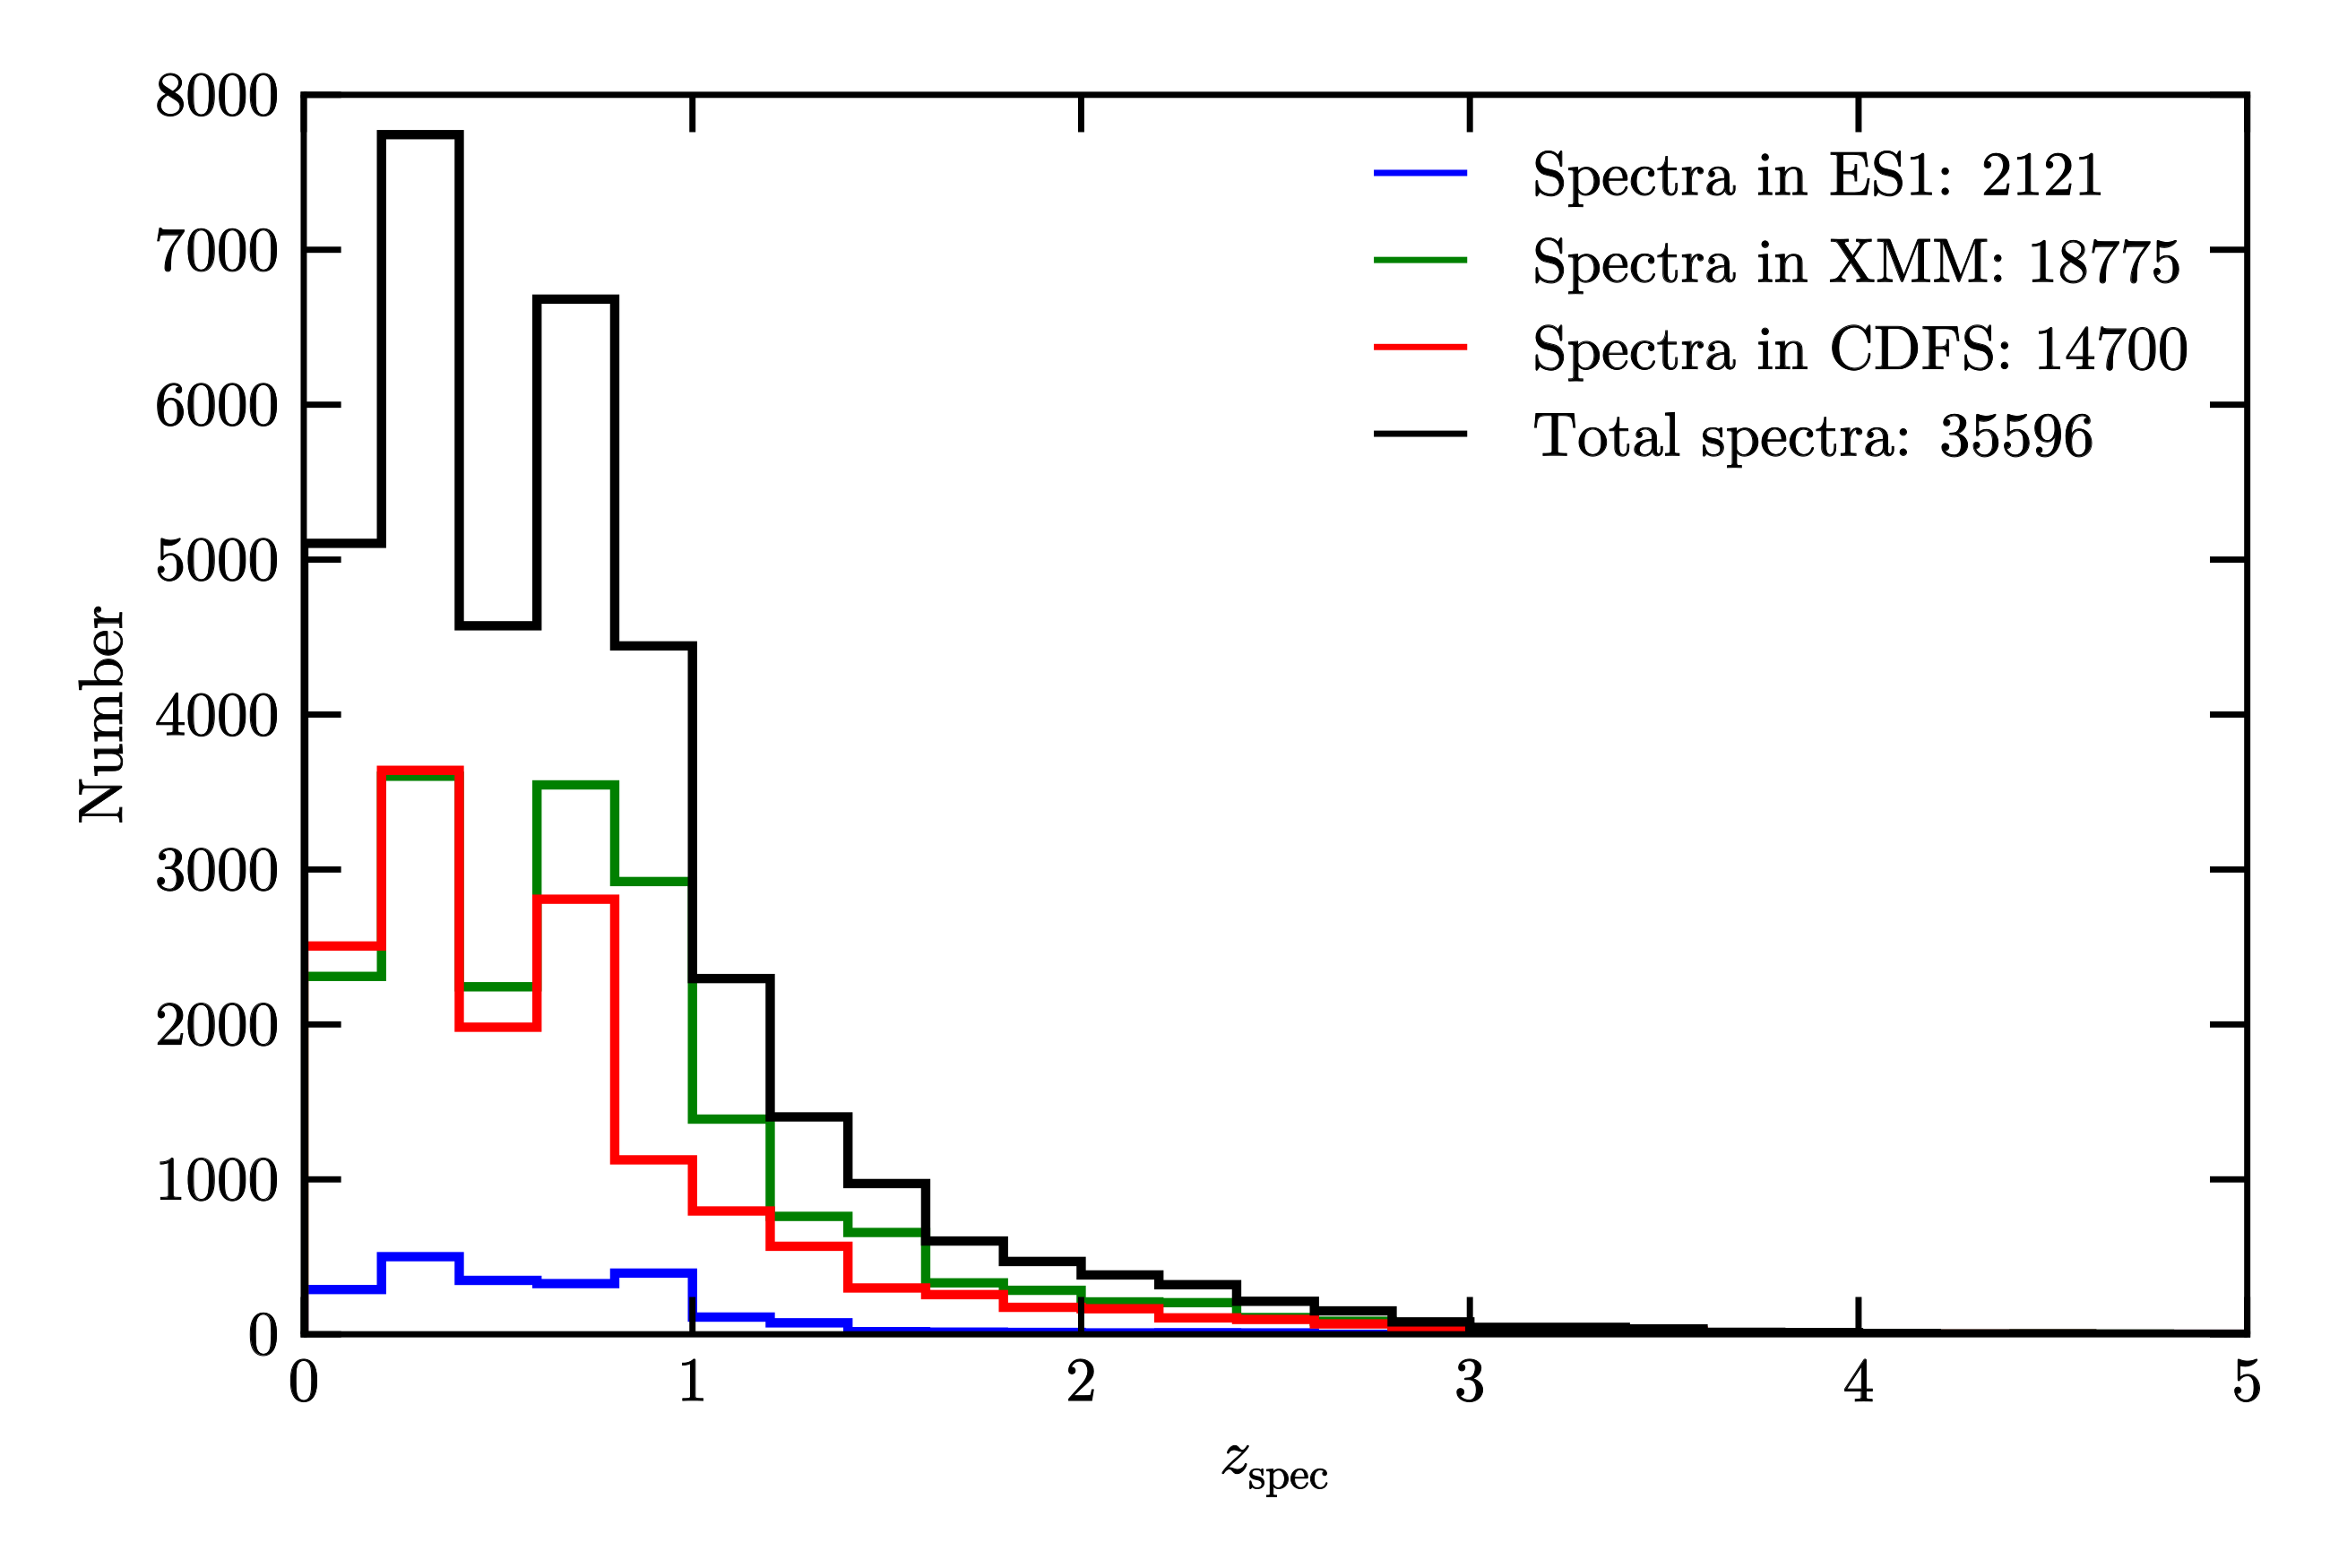
\includegraphics[width=0.95\textwidth]{spectra.png}
\caption[\texorpdfstring{$z_{\mathrm{spec}}$}{} distribution of available spectroscopic redshifts]{Spectroscopic redshift distribution of all spectra in the \DESVIDEO catalogue. The red, blue, and green histograms show the contributions from the ES1, XMM, and CDFS fields respectively, and the black histogram shows the combined distribution of all spectra. All histograms are plotted in redshift bins of $\Delta z_{\mathrm{spec}} = 0.2$.}
\label{fig:spectra}
\end{figure}






%********************************** %Fourth Section  **************************************
%\DESVIDEO CATALOGUE DOES ERRORS PER TILE. NOTE THAT THIS IS AN IMPROVEMENT OVER VIDEO CATALOGS, BECAUSE THEY DO IT PER FIELD. 

%Now the DES and VIDEO datasets have been introduced, the upcoming part of this chapter will describe how these surveys were merged into a single combined catalogue.

%\footnote{In fact, thanks to the slightly smaller PSF, the VIDEO resolution is actually somewhat better.}

\section{Forced photometry and catalogue production}\label{section:forced_photometry}
\subsection{Motivation}\label{subsection:forced_phot_motivation} Now the DES and VIDEO datasets have been introduced, the upcoming part of this chapter will turn to the next step: merging these surveys into a single combined catalogue. The most straightforward way to achieve this merger would simply be to match the existing DES and \cite{2013MNRAS.428.1281J} VIDEO catalogues by position. However, the high quality of the DES data makes it possible to do better. By using a so-called \textit{forced photometry} approach, this thesis aims to extract more information from the VIDEO imaging than is possible with VIDEO alone. The concept behind forced photometry is to use imaging from a deeper or higher resolution survey to improve the photometry and positions that can be measured from shallower or lower resolution data \citep{2015MNRAS.446.2523B, 2016AJ....151...36L}. In the case of DES and VIDEO, the two surveys have fairly similar resolutions, so the potential for improvement mainly revolves around the higher depths in the DES imaging. As demonstrated in Table \ref{table:VIDEO_depths}, the VIDEO $Z$-band data reaches depths of $24.8<Z_{\mathrm{AB}}<25.3$. While this is similar to the $z_{\mathrm{AB}}<24.9$ DES depths over the majority of the \DESVIDEO footprint, the \SI{4.3}{\sqdeg} deepest DES regions extend to $z<26.2$, which is considerably deeper. Additionally, the combined $r+i+z$ is deeper than the $z$-band alone, as it enjoys the combined exposure times from the $r$, $i$ and $z$ imaging. Therefore, it is possible to use the deeper DES imaging to obtain secure detections for objects that would be too faint to pass the detection threshold in the VIDEO imaging alone. By extracting forced photometry from VIDEO based on these secure DES detections, the VIDEO measurements can be pushed to fainter magnitudes, increasing the number of sources with measured VIDEO fluxes. The concept is illustrated in Figure \ref{fig:forced_photometry_des_cat}, which shows the increase in VIDEO measurements that can be achieved with forced photometry based on DES. Furthermore, in addition to the fact that it allows VIDEO fluxes to be obtained for fainter sources, forced photometry has a second benefit for this thesis. As mentioned in Section \ref{subsubsection:data_reduction}, the optical component of the \DESVIDEO catalogue consists of the DESDM catalogues. In order to maximise the amount of information contained within the combined catalogue, it is important to obtain VIDEO photometry for as many of these DESDM sources as possible. Forced photometry helps to achieve this objective, because it can measure VIDEO fluxes for all sources detected in DES. \par  


To extract the forced photometry and to merge it with DES data, the author has created an automated pipeline. The rest of this section will describe this pipeline and the catalogue assembly process in general. The first part will present the implementation of forced photometry, the second part will report on the validation of this method, and the third part will describe the derivation corrected photometric uncertainties for the catalogue. Then, after these parts have identified and verified the necessary steps, the fourth section will summarise the automated pipeline to produce the desired \DESVIDEO catalogue. \par



\begin{figure*}[!htpb]
\centering
\subfloat[DES detection\label{fig:forced_photometry_des_det}]{
	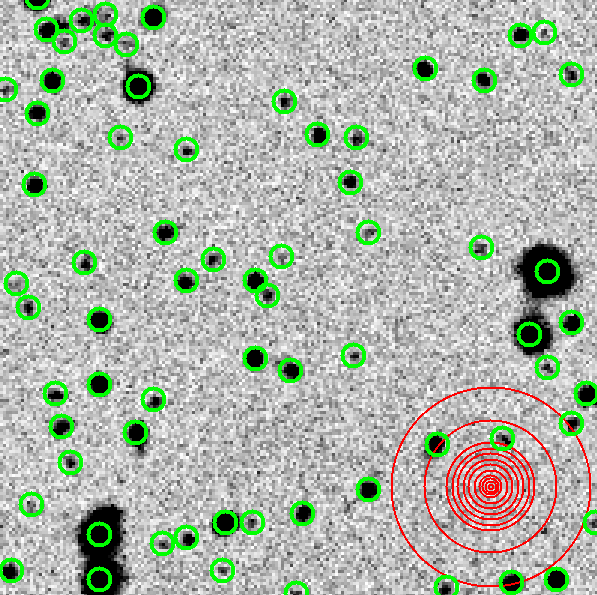
\includegraphics[clip, width=0.32\textwidth]{Chapter2/Figs/des_det_cdfs_cut.png}}
\subfloat[\DESVIDEO]{
	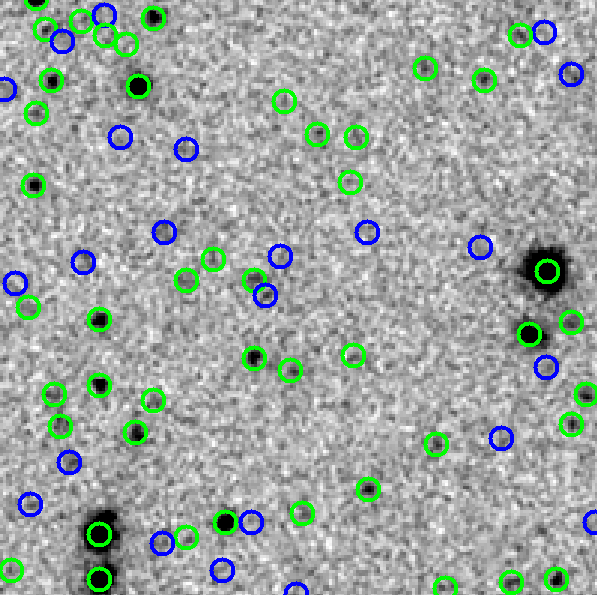
\includegraphics[clip, width=0.32\textwidth]{Chapter2/Figs/video_Z_cdfs_cut.png}}
\subfloat[VIDEO only]{
	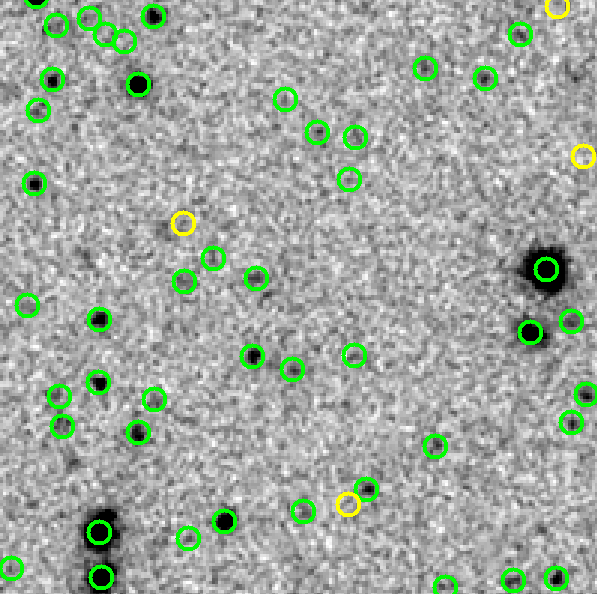
\includegraphics[clip, width=0.32\textwidth]{Chapter2/Figs/video_Z_cat_cdfs_cut.png}}
\caption[Forced photometry]{An illustration of the effectiveness of forced photometry in a section of the CDF-S where the DES data is significantly deeper than VIDEO. \textbf{(a)} DES $r+i+z$ detection image with \SI{1.95}{\arcsec} apertures centred on DES $r+i+z$ detections. All twelve aperture sizes in the \DESVIDEO catalogue (see Table \ref{table:aperture_sizes}) are superimposed to scale in red. \textbf{(b)} VIDEO $Z$-band image with DES detections from (a). The blue circles show sources which are detected in DES but not included in the VIDEO \cite{2013MNRAS.428.1281J} catalogue. \textbf{(c)} VIDEO $Z$-band image with detections from the \cite{2013MNRAS.428.1281J} VIDEO catalogue, based on the longest wavelength detection in the VIDEO $Y$-, $J$-, $H$- or $K_{s}$-band. Sources which are included in the \cite{2013MNRAS.428.1281J} catalogue but not detected in DES are shown in yellow. The abundance of blue circles compared to yellow circles illustrates that by using the deeper DES data, photometry can be obtained for VIDEO sources that are too faint to be detected in the VIDEO imaging.}
\label{fig:forced_photometry_des_cat}
\end{figure*}

%because the forced photometry is eventually measured per DES co-add tile...

\subsection{Method}\label{subsection:forced_phot_preparation}
\subsubsection{Image resampling and preparation}\label{subsubsection:image_resampling}
Before forced photometry can be extracted, the imaging must be suitably prepared. In the \DESVIDEO combination pipeline, this is achieved in the following way. Because the pipeline eventually measures forced photometry per DES co-add tile --- for every combination of intersecting DES and VIDEO tiles --- every VIDEO tile that overlaps a given DES tile is resampled to match the position, pixel scale, and size of that DES tile. This is achieved via \texttt{SWarp} v.2.38.0 \citep{2002ASPC..281..228B,2010ascl.soft10068B}, using a \texttt{LANCOS3} kernel to rescale the VIDEO data from the VIDEO pixel scale of \SI{0.2}{\arcsec.pix^{-1}} to the DES scale of \SI{0.263}{\arcsec.pix^{-1}}. Resampling is performed for every available VIDEO filter, and the \texttt{SWarp} configuration file used for this process is shown in Appendix \ref{appendix:swarp}. The result is a series of VIDEO tiles covering the same \SI{0.73 x 0.73}{\sqdeg} regions as the corresponding DES tiles. If a VIDEO tile does not fully overlap a given DES tile, \texttt{SWarp} sets the pixel values in the image and weight map to 0 in the areas where no VIDEO data is present. \par 


For the DES imaging, preparation requires consideration of the overlap pattern between the DES and VIDEO tiles. There are two special cases, which are both addressed by the pipeline. The first case applies if a DES tile is not fully contained within a given VIDEO tile, i.e. if it lies on an edge. For those tiles, the pipeline trims the DES $r+i+z$ detection image to the size of the overlapping VIDEO image. The second case concerns DES tiles where there is data from multiple VIDEO tiles. In those tiles the pipeline duplicates the detection image for each VIDEO tile and cuts  the duplicates down to the overlapping regions. This trimming is performed based on the resampled VIDEO $K_{s}$-band weight map, which was chosen because it is observed in every tile. After overlap has been accounted for, the pipeline then finishes the data preparation by assigning a value of \texttt{NaN} to all DES detection image pixels for which the corresponding VIDEO weight map pixels are zero. These zero weights occur a) for regions at the very edge of the VIDEO tile where there are no observations, b) for regions in the resampled VIDEO tiles where there is no overlapping DES data (see the previous paragraph), and c) for regions covered by the faulty detector 16 (see Section \ref{subsubsection:data_quality_video}). This approach ensures that all detected sources lie within DES regions that overlap existing and reliable VIDEO data, since the forced photometry code does not allow detected sources to contain \texttt{NaN} values. \par 


\subsubsection{Source extraction}\label{subsubsection:forced_phot_extraction}
As explained previously in Section \ref{subsection:forced_phot_motivation}, one of the advantages of forced photometry is that it can allow VIDEO fluxes to be measured for a maximum number of sources in the DESDM catalogues. To make full use of this strength, the \DESVIDEO catalogue pipeline must therefore replicate the DESDM source detection process as closely as possible, so that the measured VIDEO objects are a close match to the DESDM objects. Unfortunately, the photometry in the DESDM pipeline was obtained with a special of \texttt{SExtractor} that the author does not have access to, so it is not possible to copy that source detection method outright. In spite of this, the author has obtained a very close approximation to the DESDM results (as will be shown in Section \ref{subsection:source_extract_validation}) via a description of the DESDM configuration file, obtained from internal communication with the DES collaboration. Together with the relevant DES, VIDEO, and \texttt{SExtractor} documentation in the literature, this internal communication helped to inform the source extraction method for the \DESVIDEO pipeline. A summary of the adopted approach is presented below. \par 

Forced photometry is extracted in every available VIDEO filter, by running \texttt{SExtractor} v.2.19.5 \citep{1996A&AS..117..393B} in dual image mode for each overlapping \DESVIDEO tile combination. This process uses the DES $r+i+z$ co-adds (prepared as described in the previous section) as detection images, and the corresponding resampled VIDEO tiles as measurement images. Appendix \ref{appendix:sextractor} shows the \texttt{SExtractor} configuration file used in this process. With this setup, \texttt{SExtractor} measures photometry through a series of steps. A summary of this process, including the configuration choices made for this thesis, is presented below. More information can be found in the \texttt{SExtractor} documentation\footnote{\color{blue} http://www.astromatic.net/pubsvn/software/sextractor/trunk/doc/sextractor.pdf}. \par

Firstly, \texttt{SExtractor} creates a background map for both the DES detection and VIDEO measurement images. To do this, it estimates the background in a grid of $16 \times 16 = 256$ pixel boxes (the value of 256 used in this thesis has been imposed via the \texttt{BACK\_SIZE} parameter). Within these boxes, pixels brighter than $3\sigma$ above the median are iteratively clipped. To account for boxes where the background is overestimated due to bright stars, median filtering is applied to the grid, using a filter size of 3 boxes (as specified by the \texttt{BACK\_FILTERSIZE} parameter). The final background maps are obtained by smoothing the grid of boxes via a bicubic-spline interpolation. The resulting maps are then subtracted from the corresponding detection and measurement images. In parallel with the background maps, \texttt{SExtractor} produces a map of the RMS background noise, which is used to scale the input weight maps to the appropriate absolute level. \par 



 %(see the \texttt{SExtractor} documentation\footnote{\color{blue} http://www.astromatic.net/pubsvn/software/sextractor/trunk/doc/sextractor.pdf} for more information)


After substracting the background, \texttt{SExtractor} convolves the detection image  with a $\num{3 x 3}$ pixel convolution kernel. This improves the detectability of faint extended sources\footnote{\color{blue} http://www.astromatic.net/pubsvn/software/sextractor/trunk/doc/sextractor.pdf} by increasing the contrast with the background noise. The kernel file \texttt{sex.conv} used in this thesis is identical to the one used for the DESDM catalogues, and contains the following elements: 

\begin{equation}
\texttt{conv} =
 \begin{bmatrix}
 1 & 2 & 1 \\
 2 & 4 & 2 \\
 1 & 2 & 1 \\
 \end{bmatrix}.
\end{equation}



\texttt{SExtractor} then identifies source detections from the convolved background-subtracted $r+i+z$ detection images. For this thesis, the algorithm considers an object detected if it consists of six or more adjacent pixels (specified via $\texttt{DETECT\_MINAREA} = 6$) with a signal-to-noise ratio of  $1.6\sigma$ ($\texttt{DETECT\_THRESH} = 1.6\sigma$) above the local background\footnote{To be more precise, the required threshold for detection is adjusted for each pixel according to the weight map, such that each pixel must be above a a threshold $t_{i}=1.5\times\sqrt{\sigma_{i}^2}$, where $i$ denotes an individual pixel and $\sigma_{i}^2$ is the variance in that pixel as determined from the weight image.}. For blended detections consisting of overlapping sources, \texttt{SExtractor} attempts to separate the detections into subcomponents using a multi-thresholding algorithm \citep{1996A&AS..117..393B}. For this thesis, a subcomponent of a composite object is considered separate if its total integrated value is greater than 0.001 of the composite (\texttt{DEBLEND\_MINCONT}=0.001), and the maximum number of subcomponents is 32 (\texttt{DEBLEND\_NTHRESH}=32). \par




For every detected object, \texttt{SExtractor} extracts photometry from the back\-ground-subtracted VIDEO measurement images. The photometry consists of two main types of measurement: 


\begin{itemize}
    \item \textbf{Aperture photometry} is measured by counting the flux of pixels inside twelve fixed-size circular apertures, with a range of diameters between \SI{0.49}{\arcsec} and \SI{17.53}{\arcsec}. A list of all the diameters is provided in Table \ref{table:aperture_sizes}. To illustrate their sizes, the apertures are superimposed on part of a DES detection image in Figure \ref{fig:forced_photometry_des_det}. The diameters have been chosen to match the ones used by DESDM, so that all \DESVIDEO fluxes are measured in the same size apertures.  \texttt{SExtractor} outputs the fluxes and magnitudes as \texttt{FLUX\_APER} and \texttt{MAG\_APER} respectively. 
    %AUTO PHOTOMETRY IS EXTRACTED VIA
    \item \textbf{Auto photometry} employs a flexible elliptical aperture scaled to encompass (most of) the flux of a given source. The method implemented in \texttt{SExtractor} follows an approach pioneered by \cite{1980ApJS...43..305K} and adapted by  \cite{1996A&AS..117..393B}. It computes the shape of the desired elliptical aperture (i.e. the ratio between the semi-major and semi-minor axes) from the second order moments of the flux distribution in the detection image. The size of the ellipse is determined by a dimensionless quantity that \texttt{SExtractor} refers to as the Kron radius $R_{\mathrm{Kron}}$, which is a product of the first moment of the flux distribution and a scale factor $k$. For this thesis, the value of $k$ and the minimum permitted Kron radius $R_{\mathrm{Kron,min}}$ are set to values of 2.5 and 3.5 respectively (via the \texttt{PHOT\_AUTOPARAMS} parameter). \texttt{SExtractor} uses $R_{\mathrm{Kron}}$ to obtain the semi-major axis $a$ and semi-minor axis $b$ of the final scaled elliptical aperture in units of pixels:
    
    \begin{align}
    a &= R_{\mathrm{Kron}} \times \texttt{A\_IMAGE} \label{eqn:semi_major}, \\
    b &= R_{\mathrm{Kron}} \times \texttt{B\_IMAGE},\label{eqn:semi_minor}
    \end{align}
    
    \noindent where \texttt{A\_IMAGE} and \texttt{B\_IMAGE} are the aforementioned shape parameters computed from the second order moments, supplied in units of pixels. If the calculated value of $R_{\mathrm{Kron}}$ for a given source is less than $R_{\mathrm{Kron,min}}=3.5$, instead of a scaled aperture \texttt{SExtractor} uses an aperture of fixed area instead (still with an elliptical shape determined from the imaging). Its area corresponds to that of a circular aperture with a radius of 7.41 pixels ($\texttt{PHOT\_AUTOAPERS} = 7.41$)\footnote{This corresponds to a diameter of \SI{1.97}{\arcsec}, roughly equal to the seeing.}. \texttt{SExtractor} saves the resulting auto fluxes and magnitudes as \texttt{FLUX\_AUTO} and \texttt{MAG\_AUTO} in the output catalogues, together with \texttt{A\_IMAGE}, \texttt{B\_IMAGE}, $R_{\mathrm{Kron}}$ (listed as \texttt{KRON\_RADIUS}), and various other shape parameters. 
\end{itemize}

\begin{table}[!htpb]
\centering
\textsc{Aperture diameters} \\
\vspace{0.1em}
\footnotesize
\begin{tabular}{lcclc}
\toprule\toprule
\multicolumn{2}{c}{Aperture size}  & &  \multicolumn{2}{c}{Aperture size} \\
(arcsec) & (pix) & & (arcsec) & (pix) \\
\midrule
0.49 & 1.85 & & 4.87 & 18.52 \\
0.97 & 3.70 & & 5.84 & 22.22 \\
1.46 & 5.55 & & 6.81 & 25.93 \\
1.95 & 7.41 & & 7.79 & 29.63 \\
2.92 & 11.11 & & 11.68 & 44.44 \\
3.90 & 14.81 & & 17.53 & 66.67 \\
\bottomrule
\end{tabular}
\vspace{1em}
\caption[Aperture diameters]{Aperture diameters for the aperture photometry in the \DESVIDEO catalogue. The aperture sizes were chosen to match those of the DESDM catalogues, so that the \DESVIDEO photometry is measured in identical apertures.}
\label{table:aperture_sizes}
\end{table}

%\paragraph{} Photometry obtained via galaxy model fitting and PSF fitting is not included in the \DESVIDEO catalogue. The reason for this is that in order to measure these quantities, \texttt{SExtractor} requires a VIDEO PSF model, which is challenging to model because of the VIDEO observing strategy. As described in Section \ref{subsubsection:data_collection_video}, the VIDEO tiles are made up of paw-prints from six offsets, each of which is consists of contributions from 16 detectors. This entails that in regions of detector overlap, data may be composed of up to 16x6 PSFs. Without PSF homogenisation, this large number of PSF 



\subsection{Source extraction method validation}\label{subsection:source_extract_validation}
It is important to confirm that the configuration in the \DESVIDEO pipeline indeed replicates the DESDM configuration as closely as possible. To verify this, the author used the \DESVIDEO setup for a single \texttt{SExtractor} run in the DES0227-0458 tile, specifying the combined $r+i+z$ image as the detection image and the DES $z$-band image as the measurement image. The current section compares the result to the DESDM catalogue in the same tile.  \par

Within the single tile that was studied, the DESDM catalogue contains \num{126 624} detected sources, whereas the \DESVIDEO method in this thesis --- let us refer to this as the `Schooneveld configuration' --- finds \num{126 980} sources. When merging these catalogues by position\footnote{Based on the \texttt{ALPHAPEAK\_J2000} and \texttt{DELTAPEAK\_J2000} output parameters.} within a \SI{1}{\arcsec} radius (permitting no duplicate matches), the total number of matches is \num{123 993}. The numbers imply that the DESDM catalogues contain 2631 objects ($\approx 2\%$) not detected by the Schooneveld configuration. Conversely, the Schooneveld setup produces 2987 sources ($\approx 2\%$) that are not present in the DESDM catalogues. Figure \ref{fig:z_flux_histogram} illustrates the difference in detections between the two methods as a function of magnitude. When the author inspected the images for the divergent detections, it became clear that these objects are clustered around bright stars. They are also mostly undetected or extremely faint in the $z$-band. This suggests that the difference is caused by small differences in the way the two source extraction methods handle the detection threshold in edge cases, which may have to do with the specifics of the background estimation. Possible explanations are the fact that the DESDM configuration used a different version of \texttt{SExtractor}, or a perhaps slightly different weights image. Nonetheless, compared to the $\sim127 000$ sources in the test tile, the number of $\sim3000$  divergent detections is very small, and it is overall reassuring that the two methods retrieve very similar sets of objects. \par


%INVISIBLE - was this a visual inspection thing in the images or just a low flux in the catalogues kinda thing?






The DESDM and Schooneveld configurations were also compared in terms of the position of the brightest pixel for each object (given by the \texttt{ALPHAPEAK\_J2000} and \texttt{DELTAPEAK\_J2000} parameters). The agreement was found to be excellent: 98.5\% of all detections have identical positions and 99.7\% differ by at most 1 pixel. This demonstrates that the forced photometry is working as desired, since it confirms that the detections in the Schooneveld configuration correspond to the same sources in the DESDM catalogues. Together, this result and the result from the previous paragraph show that the Schooneveld and DESDM configurations retrieve largely the same sources, almost entirely in exactly the same positions. Therefore, it is concluded that the Schooneveld configuration can indeed achieve the aim of obtaining VIDEO photometry for a maximal number of DES sources. \par  


Additionally, Figure \ref{fig:z_flux_compare} illustrates that the Schooneveld configuration also retrieves similar photometry to the DESDM configuration. It is suspected that any discrepancies are  largely due to the fact that the DESDM pipeline possibly uses a slightly different background estimation procedure. Because \texttt{SExtractor} obtains its photometry from the background-subtracted images, magnitudes are sensitive to the specifics of the subtraction process. This suspicion is corroborated by the observation that sources with a magnitude difference of $z_{\mathrm{AB,Schooneveld}}-z_{\mathrm{AB,DESDM}}>0.01$ preferentially reside in regions where the \texttt{SExtractor} \texttt{BACKGROUND} parameter diverges between the two catalogues. \par 

\begin{figure}[h] 
\centering    
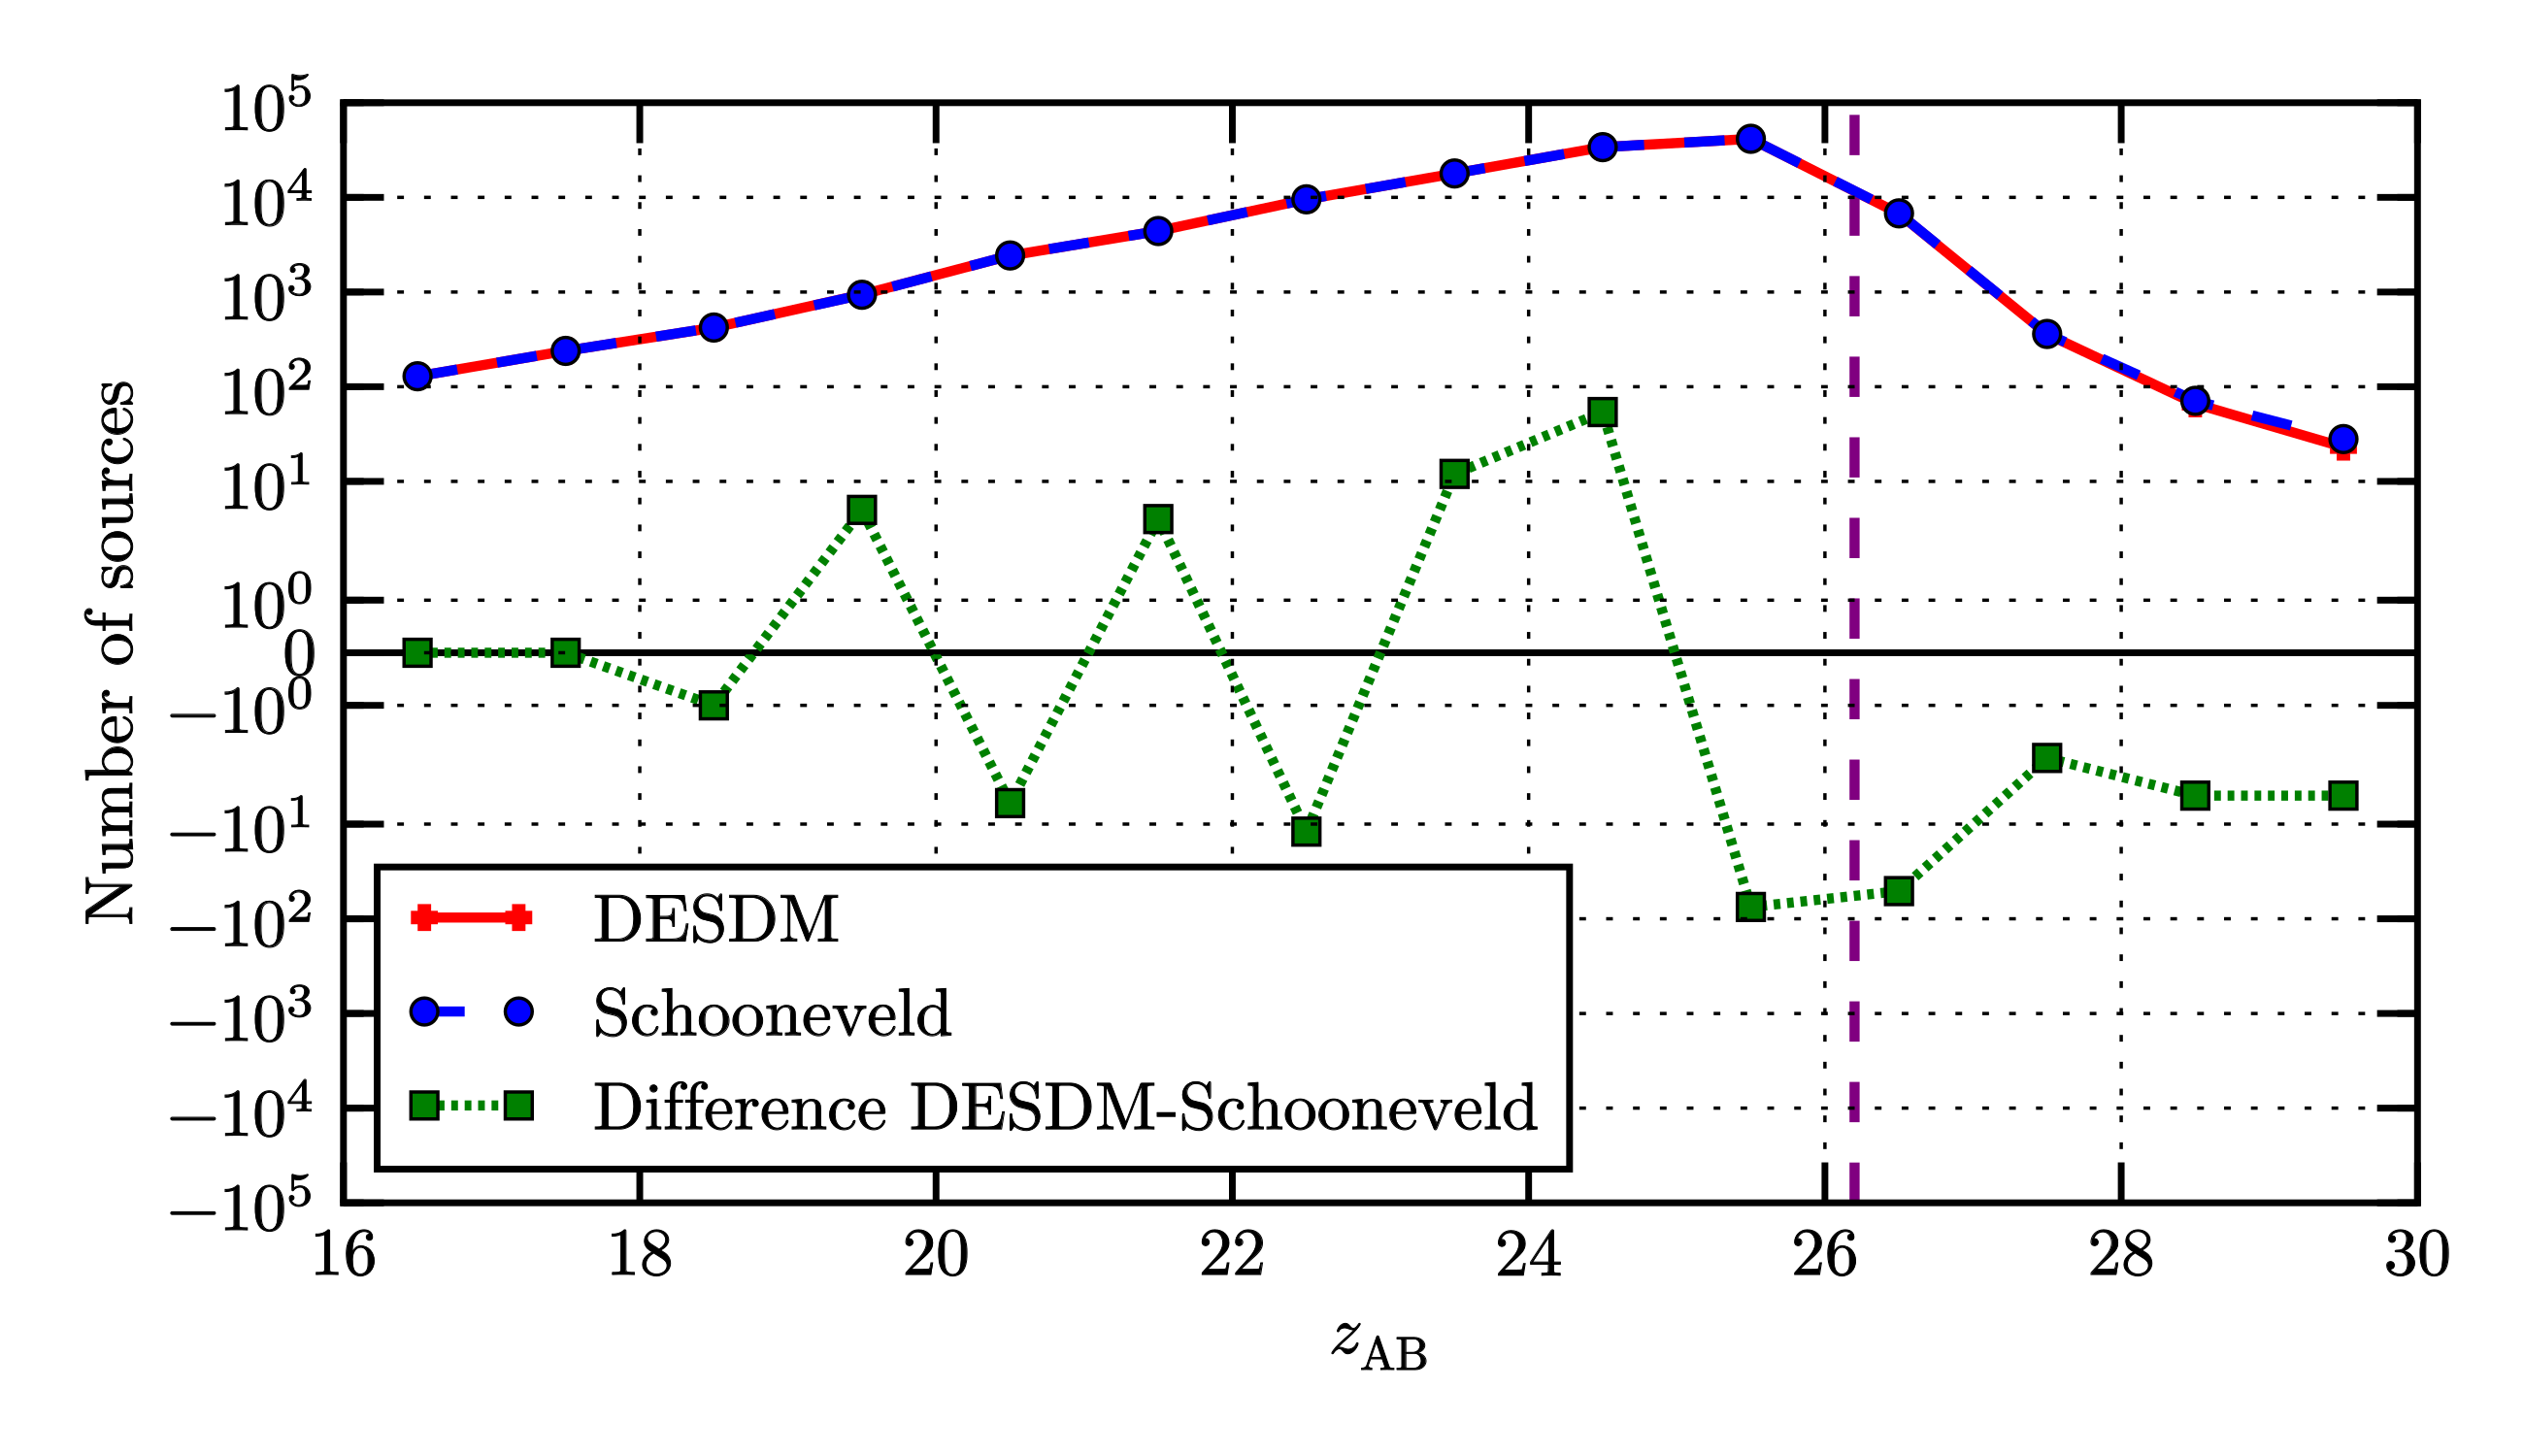
\includegraphics[width=0.95\textwidth]{z_flux_histogram.png}
\caption[Verification of the photometry method: number of source detections]{$z$-band magnitude in a \SI{1.95}{\arcsec} diameter aperture versus number of detections in bins of \SI{1}{\mag}, for detections in the DES0227-0458 tile only. Blue pluses show data from the DESDM catalogues. Green squares show the Schooneveld configuration results, from a single \texttt{SExtractor} run with the \DESVIDEO configuration used in this thesis, as described in the text. The difference between these data points is shown in red. The vertical purple dotted line shows the mean $5\sigma$ depth in the DES0227-0458 tile.}
\label{fig:z_flux_histogram}
\end{figure}


\begin{figure}[h] 
\centering    
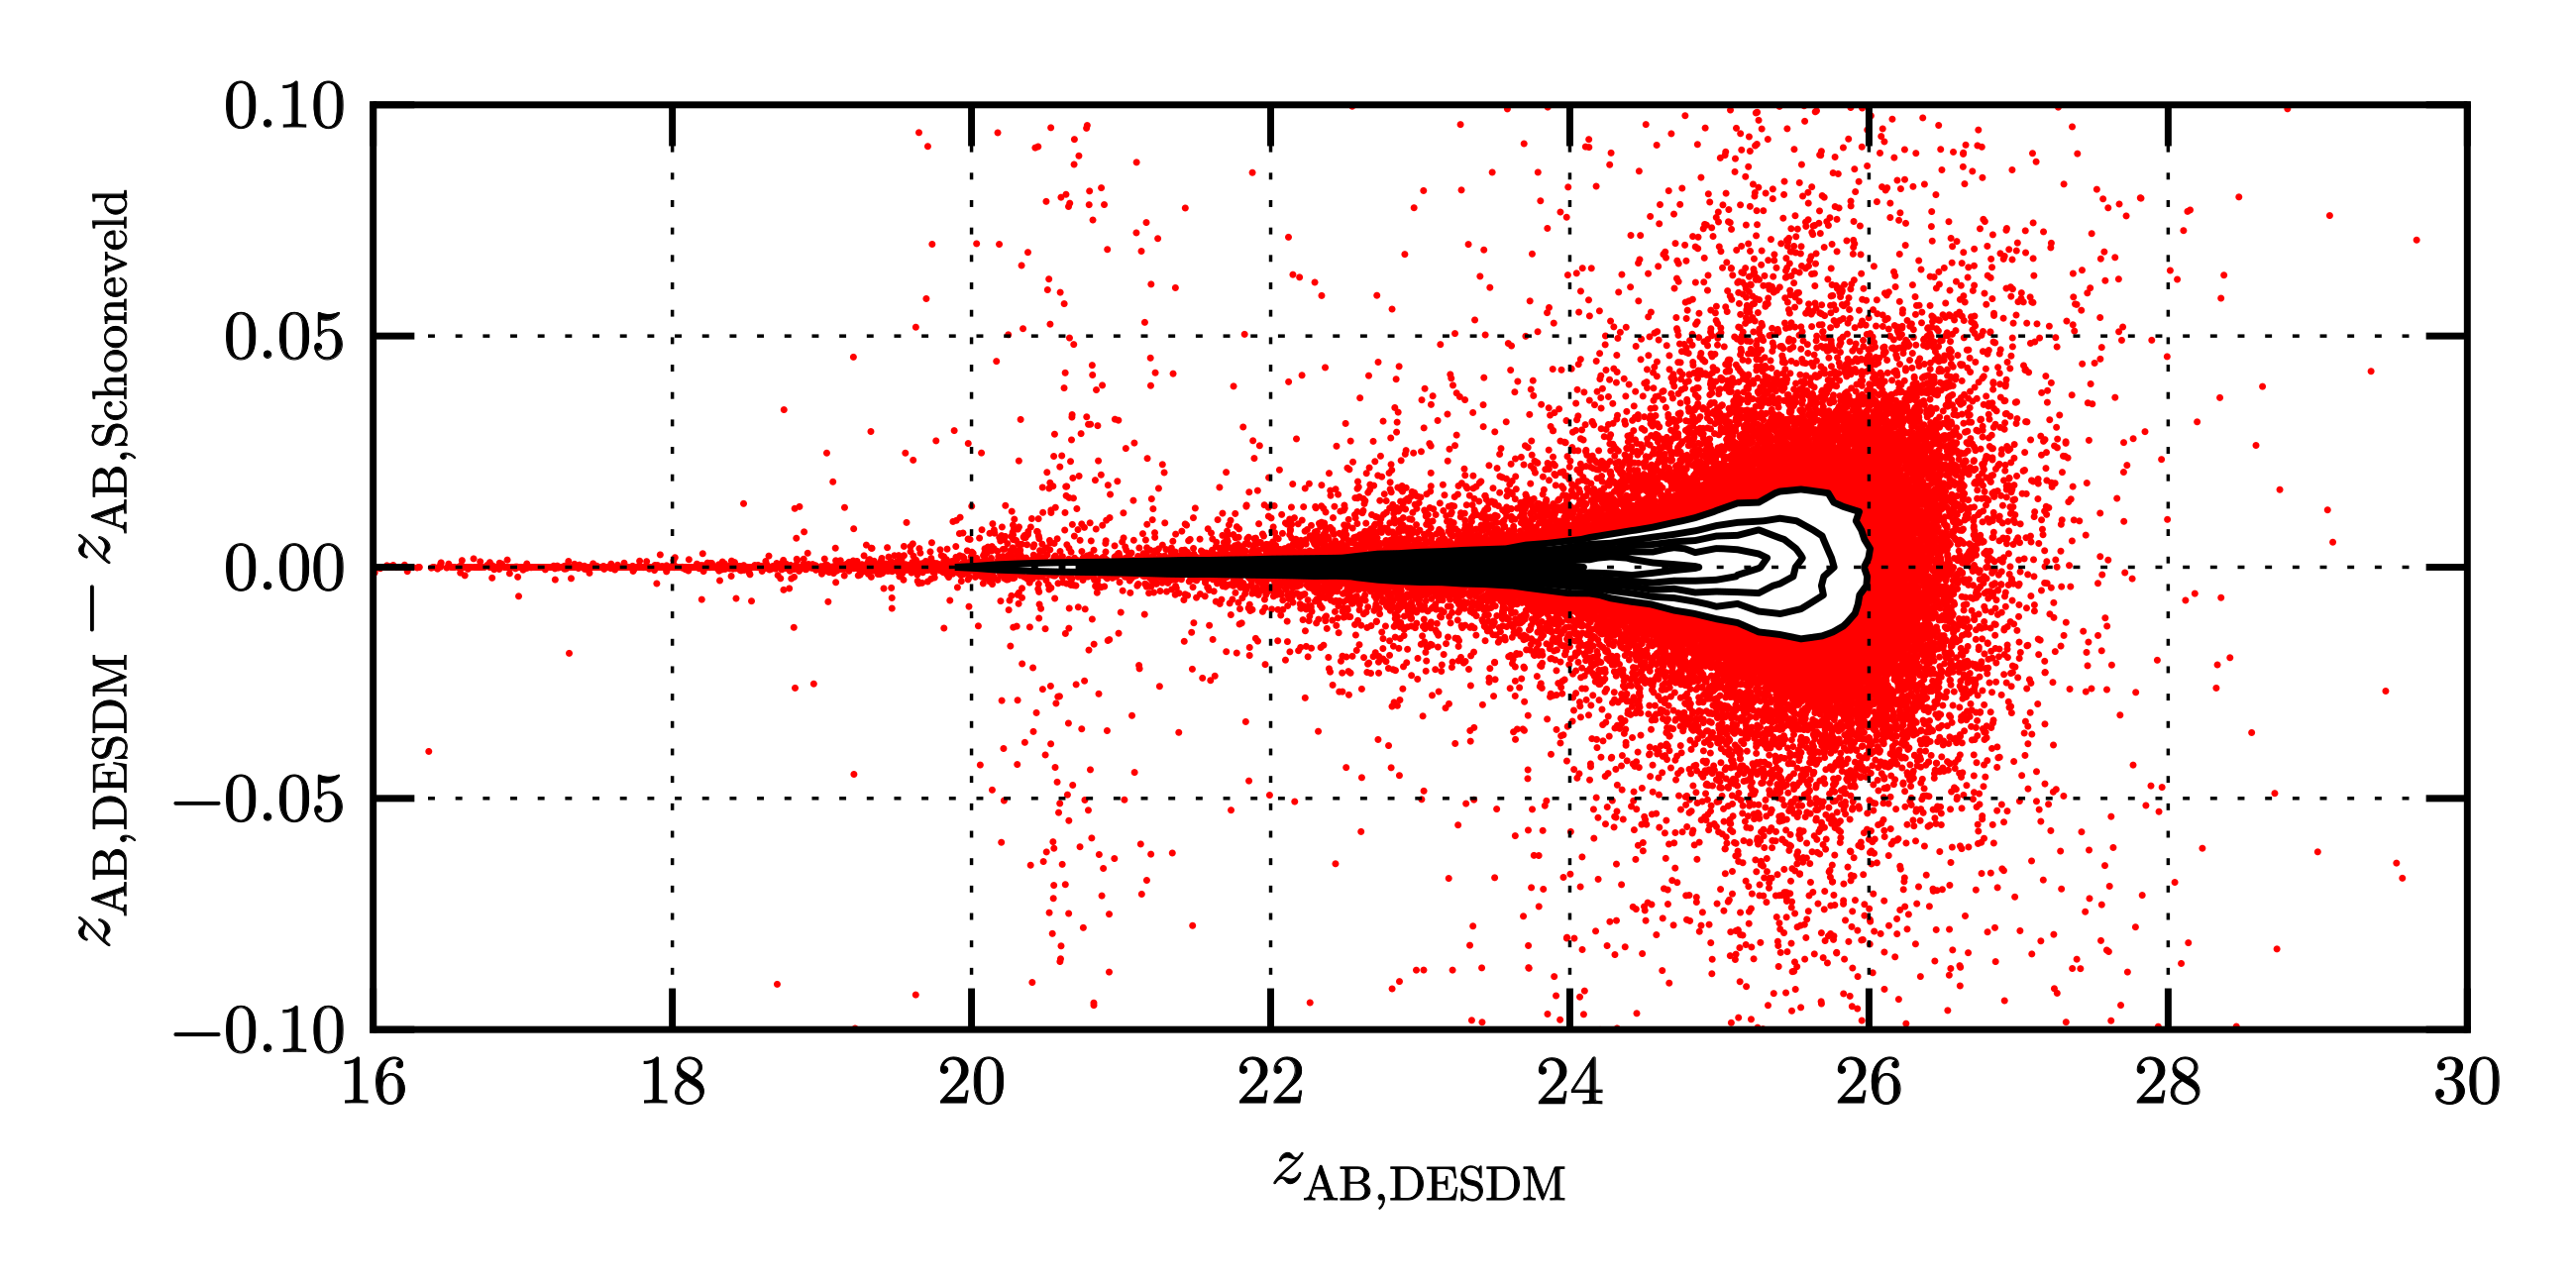
\includegraphics[width=0.95\textwidth]{z_flux_compare.png}
\caption[Verification of the photometry method: photometry]{Difference in $z$-band magnitude in a \SI{1.95}{\arcsec} diameter aperture between the DESDM configuration and the Schooneveld configuration, plotted as a function of DESDM magnitude. Both configurations contain data from the DES0227-0458 tile only. The Schooneveld configuration consists of a single \texttt{SExtractor} run with the \DESVIDEO configuration used in this thesis, as described in the text. Each plotted point corresponds to an object common to both outputs.}
\label{fig:z_flux_compare}
\end{figure}


All in all, the good degree of agreement in all three of the above tests implies that the source extraction method in this thesis is adequate for the purpose of obtaining forced photometry for the \DESVIDEO catalogue. \par 



\subsection{Correction of the VIDEO photometric uncertainties}\label{subsection:errors}
Before the VIDEO forced photometry can be incorporated into the \DESVIDEO catalogue, its uncertainties must be adjusted to the correct values. The photometric noise properties estimated by \texttt{SExtractor} assume that images are made up of uncorrelated pixels, so that the noise follows a Poisson distribution. As a result, the uncertainties listed in the \texttt{SExtractor} output catalogues are simply based on the pixel-to-pixel rms. However, this assumption of uncorrelated noise is not valid for the VIDEO images, as they have been resampled several times. The VIDEO survey data reduction process (see Section \ref{subsubsection:video_data_reduction}) initially rescaled the images from the VIRCAM pixel scale of \SI{0.339}{\arcsec.pix^{-1}} to the VIDEO co-add scale of \SI{0.2}{\arcsec.pix^{-1}}, and the resampling for this thesis (described in Section \ref{subsubsection:image_resampling}) has further rescaled the imaging to the \SI{0.263}{\arcsec.pix^{-1}} DES pixel scale. In both instances, this process has introduced correlations between pixels, which means that the  \texttt{SExtractor} errors are expected to give an inaccurate representation of the true VIDEO uncertainties (see e.g.  \citealt{2003AJ....125.1107L} and \citealt{2006ApJS..162....1G} for a demonstration that correlated fluxes lead to incorrect \texttt{SExtractor} errors). \par

 

To obtain a more accurate measure of the VIDEO errors, the author has computed the correct uncertainties via a technique developed by \cite{2003AJ....125.1107L} and \cite{2006ApJS..162....1G}, which is commonly applied in the literature (e.g. \citealt{2007AJ....134.1103Q,2011ApJ...735...86W,2013ApJS..206....8M,2013MNRAS.428.1281J}). Conceptually, this approach involves measuring the flux inside a large number of  fixed-size apertures placed randomly in empty regions of the image. The distribution of fluxes within these apertures can be approximated by a Gaussian curve. The true photometric error, which corresponds to the  background noise, can then be computed from the standard deviation of this Gaussian. \par 

Before the discussion will move on to applying this method to the data, it is important to note that correlated noise is not an issue for the DES uncertainties. Because the DES co-add pixel scale of  \SI{0.263}{\arcsec.pix^{-1}} is identical to that of the DECam CCDs, the DESDM data reduction process described in Section \ref{subsubsection:data_reduction} did not need to apply any rescaling to resample the DECam exposures into the DES co-adds. This means that the co-addition introduced only minimal flux correlations, exclusively from stacking with \texttt{SWarp}. As a result, the original \texttt{SExtractor} errors in the DESDM catalogues indeed closely capture the true photometric uncertainties, and no corrections are required. \par



\subsubsection{Aperture flux errors}\label{subsubsection:aperture_flux_errors}
The above method for correcting the VIDEO uncertainties has been implemented via a custom code developed by the author. In this algorithm, errors are calculated for each VIDEO tile and filter individually, following a process that will now be described below. Firstly, the error-calibration pipeline creates a segmentation image for each VIDEO co-add tile\footnote{For clarity, these are the original VIDEO data products presented in Section \ref{subsubsection:video_data_reduction}, before the resampling and cutting up by the \DESVIDEO pipeline described in Section \ref{subsubsection:forced_phot_extraction}.} via \texttt{SExtractor}, using essentially\footnote{The only thing that needed to be changed in the input files are the values specified for the aperture diameter, since these must be supplied in pixels. Because the VIDEO tiles have a pixel scale of \SI{0.2}{\arcsec.pix^{-1}}, the aperture sizes in these  \texttt{SExtractor} runs are scaled by a factor of $0.2/0.263=0.760$ compared to the values listed in Table \ref{table:aperture_sizes} and Appendix \ref{appendix:sextractor}. The true size of the apertures (i.e. the size in arcsec) remains the same.} the same configuration as described in Section \ref{subsubsection:forced_phot_extraction} and Appendix \ref{appendix:sextractor}.  In such segmentation maps, \texttt{SExtractor} assigns an integer value to pixels designated as part of a detected object, and a value of zero to all other pixels. An example region of such a segmentation map is shown in Figure \ref{fig:segmentation}. To identify empty regions, the pipeline firstly randomly chooses \num{500000} positions on the segmentation map. For a given aperture size the code then selects a random subset of \num{10000} positions with empty apertures (i.e. not encircling any non-zero pixels that overlap a detected object), which it uses to extract the required background fluxes from the VIDEO co-add tiles. For each tile and filter, the random selection of \num{10000} empty apertures from the \num{500000} random positions and the subsequent photometry procedure is executed seven times --- once for each of the first seven aperture sizes in Table \ref{table:aperture_sizes} (i.e. with diameters between \SI{0.49}{\arcsec} and \SI{4.87}{\arcsec}). The larger apertures are omitted, because these are more likely to encircle some low surface brightness sources just below the detection limit and are thus less reliably truly empty. Fluxes from random apertures on the very edge of a given tile (where the pixel flux values are zero) are then removed by rejecting any fluxes that equal exactly zero. The result is a series of just under\footnote{The numbers ended up as slightly less than \num{10000} because of the rejected fluxes from apertures that happened to lie on the very edge of a tile.} \num{10000} fluxes in random empty apertures for every VIDEO tile, VIDEO filter, and aperture size. \par

\begin{figure}[!tpb] 
\centering    
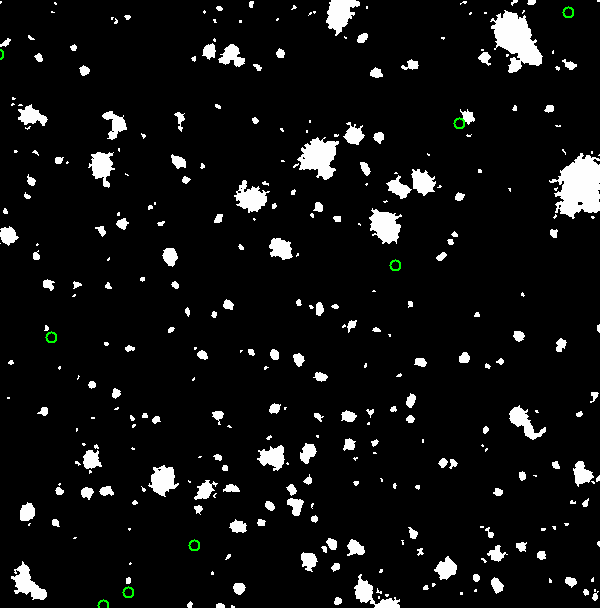
\includegraphics[width=0.45\textwidth]{aperture_errors.png}
\caption[Segmentation image]{Segmentation image for the VIDEO $K_{s}$-band in the xmm3 tile, with \SI{1.95}{\arcsec} apertures randomly placed in empty regions. The white areas consist of pixels that \texttt{SExtractor} has assigned to a detection. For the purpose of error estimations, apertures are designated as empty if they do not encircle any of these pixels.}
\label{fig:segmentation}
\end{figure}


\begin{figure*}[!tpb]
\centering
\subfloat[Flux distribution\label{fig:flux_fitting_distribution}]{
	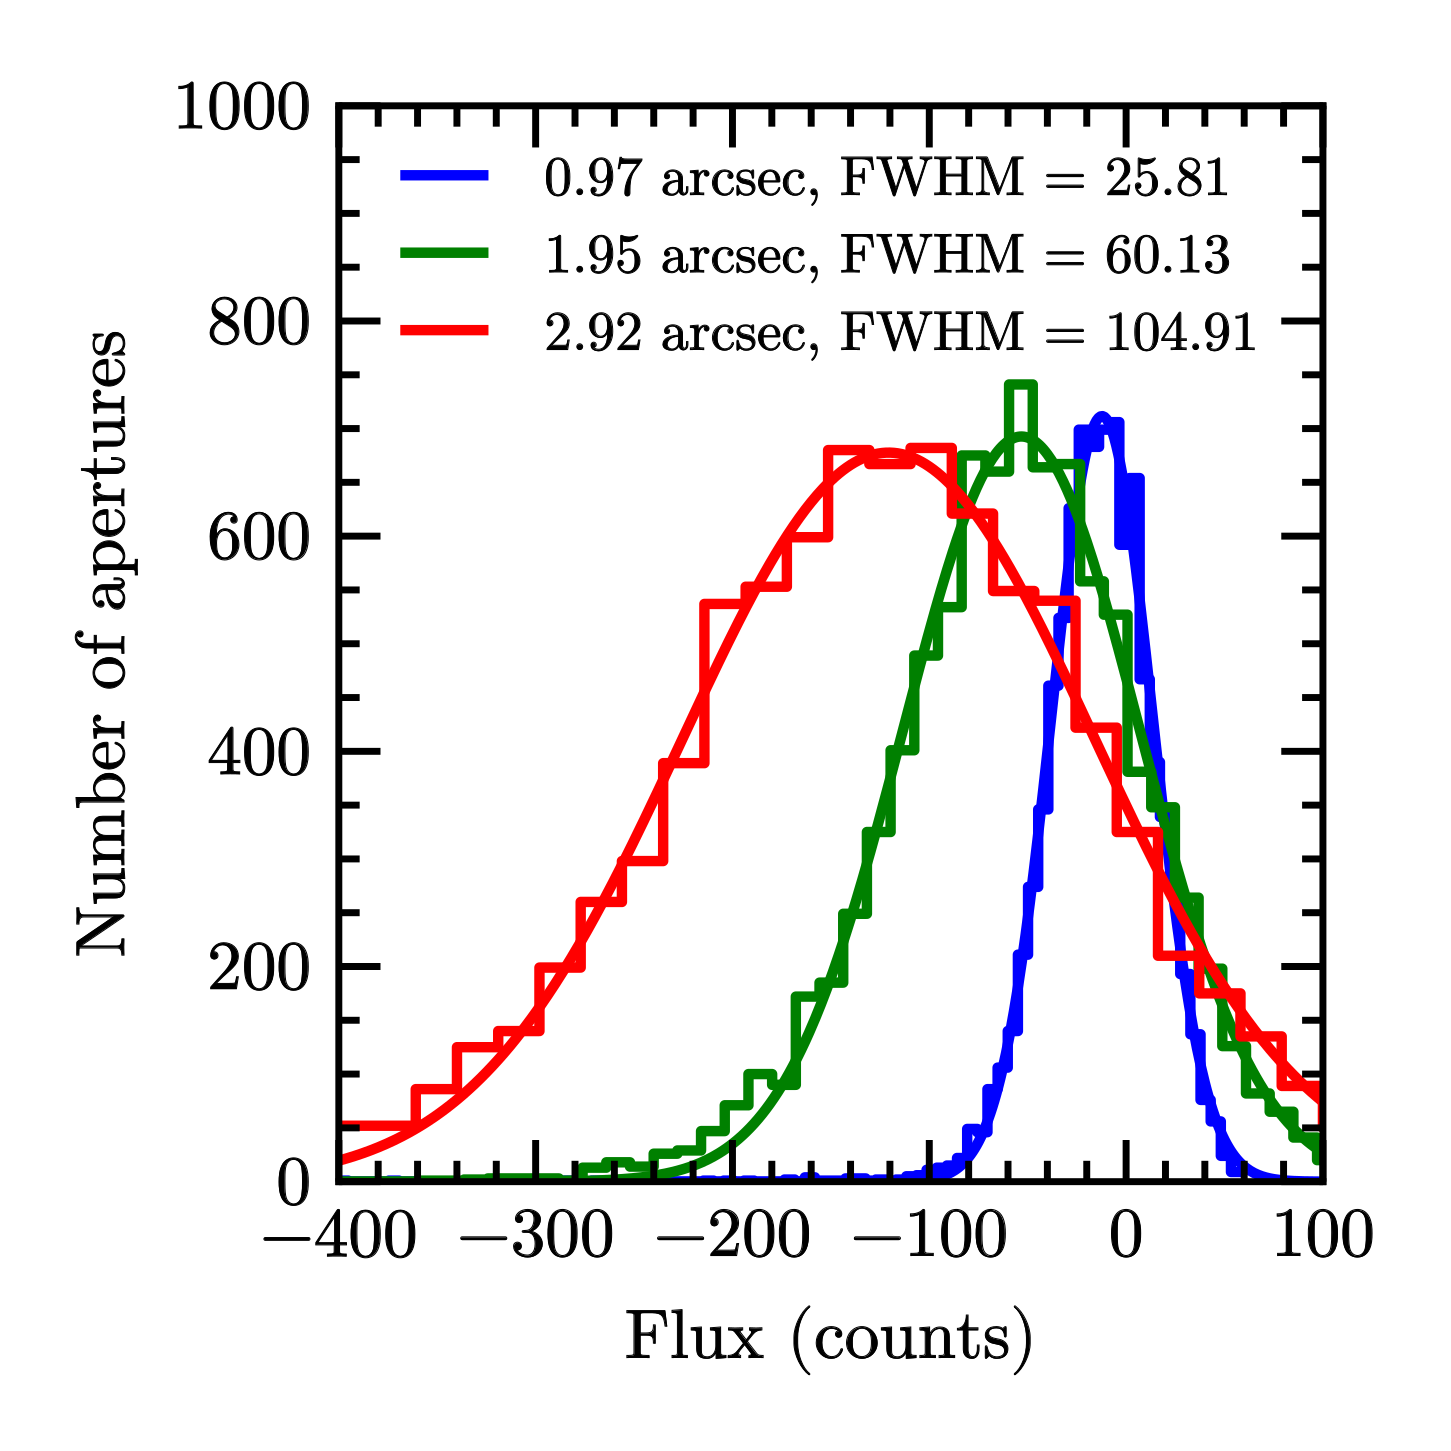
\includegraphics[clip, width=0.50\textwidth]{Chapter2/Figs/error_histogram.png}}
\subfloat[Radius dependence\label{fig:flux_fitting_radius}]{
	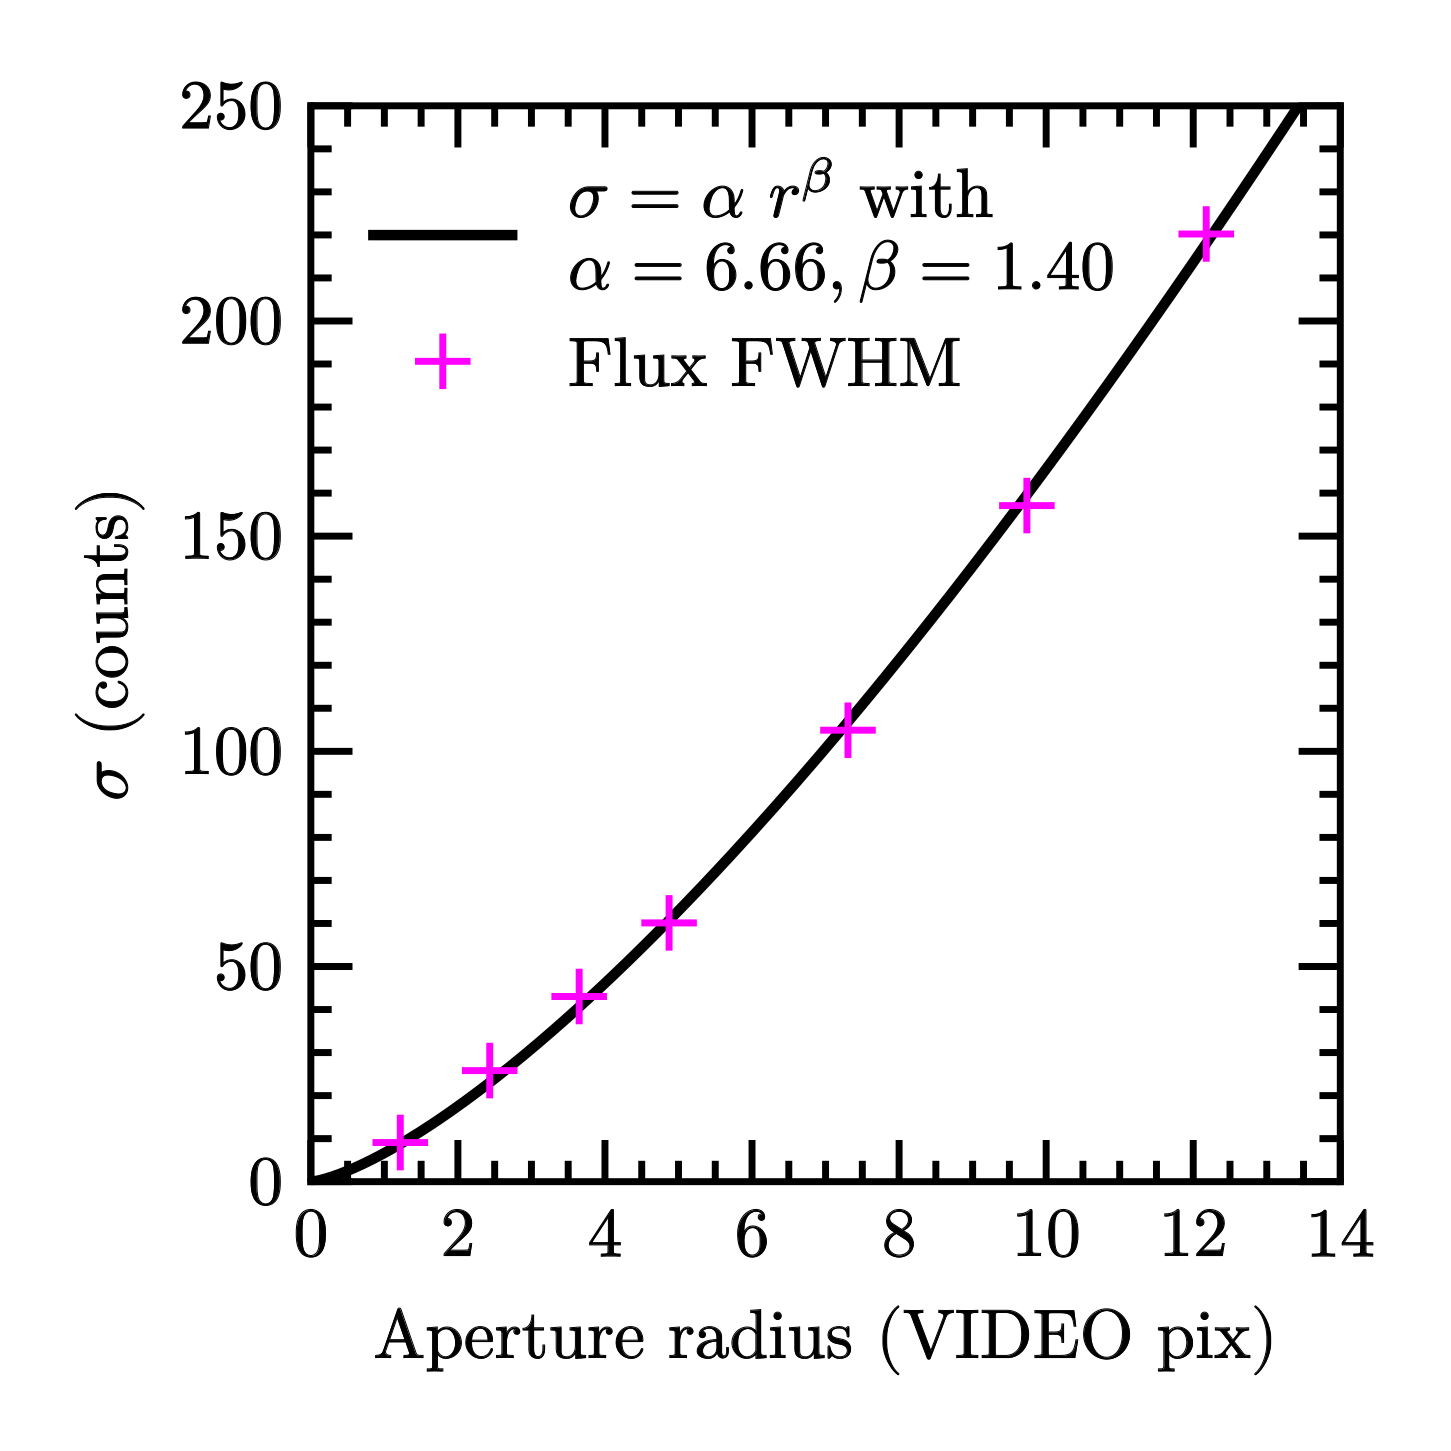
\includegraphics[clip, width=0.50\textwidth]{Chapter2/Figs/error_plot.png}}
\caption[Error estimation procedure]{An illustration of the two-part fitting algorithm to estimate VIDEO photometric errors, showing results for the $K_{s}$-band in the xmm3 tile. \textbf{(a)} Histograms of flux distributions for three of the seven measured apertures (i.e. 0.97, 1.95, and \SI{2.92}{\arcsec}; in blue, green, and red respectively), binned in intervals adjusted proportionally to the standard deviation. Each distribution has been fitted to a Gaussian, which is overplotted. For each aperture size, the measured background error $\sigma$ is equal to the Gaussian FWHM listed in the legend. \textbf{(b)} The background error $\sigma$  for all seven \SIrange{0.49}{4.87}{\arcsec} apertures as a function of aperture radius. The values of $\sigma$ (shown in pink pluses) have been computed via the Gaussian fitting prodecure illustrated in (a). Radii are given in the pixel scale of the VIDEO tiles (i.e. \SI{0.2}{\arcsec.pix^{-1}}), and the apertures from (a) correspond to the second, fourth, and fifth data points from the left.  The values of $\sigma$ have been fitted to a power law $\sigma=\alpha \ r^{\beta}$ to obtain values for $\alpha$ and $\beta$. The power law for the best-fit values of $\alpha$ and $\beta$ is shown in black. This power law is then used to calculate the final errors for all twelve \DESVIDEO aperture sizes.}
\label{fig:flux_fitting}
\end{figure*}


For each tile, filter, and aperture size, the pipeline fits a Gaussian curve to the distribution of fluxes. Figure \ref{fig:flux_fitting_distribution} illustrates this process, showing the results for the 0.97, 1.95, and \SI{2.92}{\arcsec} apertures in the xmm3 $K_{s}$-band. The standard deviation $\sigma$ of the fitted Gaussians corresponds to the desired quantity, i.e. the background error in a given aperture. It is reassuring that upon visual inspection of the pipeline fits, all the measured flux distributions were found to be fitted well by a Gaussian, as expected if the method in the \DESVIDEO pipeline indeed measures the background noise in empty regions \citep{2003AJ....125.1107L,2006ApJS..162....1G}. \par  


Up to this point, the error-estimation algorithm can successfully compute the background error for each tile and filter in the seven smallest aperture sizes. To smooth out the effects of random aperture selection for these seven sizes, as well as to obtain uncertainties for the five largest aperture sizes, the background error $\sigma$ is expressed as a function of aperture radius, from which  maximally reliable errors for all twelve aperture sizes can be interpolated and extrapolated.  Following \cite{2006ApJS..162....1G} and \cite{2011ApJ...735...86W}, this dependence of $\sigma$ on the aperture radius $r$ is parameterised by a power law: 

\begin{equation}
\sigma = \alpha \ r^{\beta}, \label{eqn:sigma}
\end{equation}

\noindent where $\beta=1$ in the case of no correlations between pixels, and  $\beta=2$ for perfect correlations. The pipeline fits this power law to the values of $\sigma$ in all seven measured apertures to obtain $\alpha$ and $\beta$. As an example, the resulting curve for the xmm3 $K_{s}$-band is shown in Figure \ref{fig:flux_fitting_radius}. Here, as well as in all other fields and filters, the output value of $\beta$ was crucially found to lie between 1 and 2, confirming the presence of correlations between pixels. \par

As a final step, the pipeline then computes the desired \DESVIDEO catalogue flux errors (\texttt{FLUXERR\_APER}) for all twelve apertures in Table \ref{table:aperture_sizes}, by inserting the best-fit parameters $\alpha$ and $\beta$ into Equation \ref{eqn:sigma}. At the same time these flux errors are also converted to magnitude errors (\texttt{MAGERR\_APER}). The resulting measurements of \texttt{FLUXERR\_APER} and \texttt{MAGERR\_APER} in every tile and filter are later used by the \DESVIDEO catalogue creation pipeline to replace the original errors computed by \texttt{SExtractor}.  \par

\paragraph{Assumptions} It is important to point out that the above process for computing the corrected VIDEO errors is based on a number of assumptions. Firstly, the error measurements assume that the uncertainties are constant within a given VIDEO tile. In practice, this is not completely true, because some parts of the tiles contain a higher or lower number of exposures than average (as described in Section \ref{subsubsection:data_quality_video}). This variation causes slight differences in the true errors, as a higher density of exposures leads to lower true background errors (and vice versa). Nevertheless, since the VIDEO coverage is reasonably uniform within each tile (as demonstrated in Figure \ref{fig:weight_map}), the assumption of constant errors is reasonably accurate. It is noted that \cite{2013MNRAS.428.1281J} have also made the same assumption. \par 

Secondly, it is assumed that the flux uncertainties can be directly equated with the background error. In reality, the true uncertainties also contain a contribution from the Poisson counting of electrons in the detectors \citep{2007AJ....134.1103Q}. However, this effect is only significant for the very brightest sources. In the \cite{2013MNRAS.428.1281J} catalogues, which do include Poisson counting, its contribution to the error only reaches >1\% at $Z_{\mathrm{AB}}<20.8$ in the $Z$-band and at $K_{s}<17.4$ in the $K_{s}$-band. The \DESVIDEO catalogue is primarily aimed at computing photometric redshifts for galaxies and finding high-redshift galaxies. Since the vast majority of these objects are significantly fainter than the threshold at which Poisson counting becomes important, the omission of the Poisson contribution is justified for the purposes of this thesis. \par 

%This threshold is much brighter than the vast majority of objects that are relevant to the objectives of the \DESVIDEO catalogue, which is aimed at computing photometric redshifts and finding high-redshift galaxies. Therefore, omitting the Poisson contribution is justified for the purposes of this thesis. 

%



\subsubsection{Auto flux errors}
In contrast to aperture photometry, which is measured in circular apertures of a fixed size, \texttt{SExtractor} measures auto photometry in elliptical apertures which are scaled to the size of each individual detection (as explained previously in Section \ref{subsubsection:forced_phot_extraction}).  By using Equation \ref{eqn:sigma}, the \DESVIDEO pipeline can also estimate accurate errors for those varying apertures. In order to do so, the error estimation code defines an `effective radius' $R_{\mathrm{eff}}$, which is the radius that corresponds to a circular aperture of the same area $A_{\mathrm{circ}}$ as the ellipse: 

\begin{equation}
    \pi R_{\mathrm{eff}} = A_{\mathrm{circ}} \equiv A_{\mathrm{ell}} = \pi a b. \label{eqn:A}
\end{equation}

\noindent Here, $A_{\mathrm{ell}}$ is the area of an elliptical aperture with semi-major and semi-minor axes $a$ and $b$. The expressions that \texttt{SExtractor} uses to calculate $a$ and $b$ have been introduced previously in Equations \ref{eqn:semi_major} and \ref{eqn:semi_minor}. Together with Equation \ref{eqn:A}, these yield:

\begin{equation}
R_{\mathrm{eff}} = \sqrt{R_{\mathrm{Kron}} \times \texttt{A\_IMAGE} \times R_{\mathrm{Kron}} \times \texttt{B\_IMAGE}}. \label{eqn:r_eff}
\end{equation}

\noindent If the Kron radius computed by \texttt{SExtractor} falls below the specified minimum value introduced in Section \ref{subsubsection:forced_phot_extraction}, the effective radius $R_{\mathrm{eff}}$ instead corresponds to that of a \SI{1.97}{\arcsec} diameter circular aperture. For each object, the error calibration pipeline computes the auto uncertainties by inserting the value of $R_{\mathrm{eff}}$ into Equation \ref{eqn:sigma}, using the best-fit parameters $\alpha$ and $\beta$ computed from the flux FWHM in circular apertures as described in Section \ref{subsubsection:aperture_flux_errors}. The resulting auto errors and corresponding magnitude errors later replace the \texttt{FLUXERR\_AUTO} and \texttt{MAGERR\_AUTO} uncertainties computed by \texttt{SExtractor}. Similarly to the aperture flux procedure, the auto flux calibration assumes that the background is constant within a tile, and that the contribution from Poisson counting is insignificant. \par 



\subsubsection{Verification of the corrected errors}\label{subsubsection:error_discussion}


\begin{table}[!p]
\centering
\textsc{\DESVIDEO errors compared to \cite{2013MNRAS.428.1281J}} \\
\vspace{0.1em}
\footnotesize
\begin{tabular}{lcccccccc}
\toprule\toprule
& \multicolumn{2}{c}{Error}  & &  \multicolumn{2}{c}{Error} & &  \multicolumn{2}{c}{Error} \\
& \multicolumn{2}{c}{(\SI{2}{\arcsec} aperture)}  & &  \multicolumn{2}{c}{(\SI{2}{\arcsec} aperture)} & &  \multicolumn{2}{c}{(\SI{2}{\arcsec} aperture)} \\
& \multicolumn{2}{c}{(counts)}  & &  \multicolumn{2}{c}{(counts)} & &  \multicolumn{2}{c}{(counts)} \\
\vspace{-0.7em}\\
\toprule
& \multicolumn{2}{c}{$Z$-band}  & &  \multicolumn{2}{c}{$Y$-band}  & &  \multicolumn{2}{c}{$J$-band} \\
Tile & Schooneveld & Jarvis &  & Schooneveld  & Jarvis & & Schooneveld  & Jarvis \\
\midrule\midrule
cdfs1 & 24.4 & 24.8 & & 31.2 & 31.3 & & 31.6 & 32.2 \\
cdfs2 & - & - & & - & - & &  44.7 & 46.5 \\
cdfs3 & - & - & & - & - & &  48.7 & 51.1 \\
es1-north & 15.3 & 14.5 & & 22.7 & 21.2 & & 56.4 & 60.6 \\
es1-south & 17.3 & 16.9 & & 27.7 & 27.1 & &  57.0 & 62.2 \\
xmm1 & 14.0 & 13.0 & & 22.6 & 21.6 & & - & - \\
xmm2 & - & - & & 22.9 & 22.2 & & 30.6 & 31.3 \\
xmm3 & 15.0 & 13.6 & & 22.6 & 21.6 & & 30.3 & 30.6 \\
\midrule
& \multicolumn{2}{c}{$H$-band}  & &  \multicolumn{2}{c}{$K_{s}$-band} \\
Tile & Schooneveld & Jarvis & & Schooneveld  & Jarvis & & &  \\
\midrule\midrule
cdfs1 & 49.7 & 51.1 & & 66.0 & 68.8 & & & \\
cdfs2 & 101.9 & 109.9 & & 73.9 & 76.3 & & & \\
cdfs3 & - & - & & 140.2 & 151.6 & & & \\
es1-north & 53.6 & 54.0 & & 63.6 & 66.0 & & & \\
es1-south & 47.2 & 47.7 & & 64.2 & 67.8 & & & \\
xmm1 & 64.2 & 67.4 & & 70.1 & 72.1 & & & \\
xmm2 & 45.8 & 47.0 & & 67.4 & 70.4 & & & \\
xmm3 & 46.8 & 48.0 & & 63.4 & 66.7 & & & \\
\bottomrule
\end{tabular}
\vspace{1em}
\caption[Comparison of photometric uncertainties]{A comparison between the VIDEO errors computed via the procedure in this thesis (labelled `Schooneveld') and the errors from the \cite{2013MNRAS.428.1281J} catalogues. The \cite{2013MNRAS.428.1281J} errors in this table include the random background error only (i.e. they do not contain the contribution from Poisson counting of electrons in the VIRCAM detectors). Dashes indicate filters which were not observed in a given tile. Since \cite{2013MNRAS.428.1281J} photometry used a \SI{2}{\arcsec} diameter aperture, the Schooneveld errors have been scaled from the DES radius of \SI{0.97}{\arcsec} to the VIDEO radius of \SI{1}{\arcsec} via Equation \ref{eqn:sigma} --- i.e. $\sigma_{\mathrm{2arcsec}} = \sigma_{\mathrm{1.95arcsec}} (1/0.97)^{\beta}$. The values of $\beta$ for each filter and tile have been derived from the best-fit parameters of Equation \ref{eqn:sigma}, which have been obtained as described in Section \ref{subsubsection:aperture_flux_errors}. The agreement between all pairs of errors is generally good, with all values agreeing within 10\% and a majority within 5\%. }
\label{table:error_agreement}
\end{table}

 

To verify that the error estimation algorithm in this thesis functions as intended, the author has compared its output to the errors in the \cite{2013MNRAS.428.1281J} catalogues (which were similarly empirically determined from the standard deviation of flux in randomly placed apertures). Table \ref{table:error_agreement} presents the results of this comparison. Reassuringly, the agreement is generally good. In all tiles and filters, the two error values agree within $<10 \%$, with most differing by less than 5\%. \par

The corrected errors were also compared to the original (uncorrected) \texttt{SExtractor} errors. The analysis revealed a considerable difference, with \texttt{SExtractor} underestimating the uncertainties by up to a factor of 2 in some filters. This observation quantitatively underlines the extent to which flux correlations introduced by image resampling can cause problematic inaccuracies in error estimations that are simply based on pixel-to-pixel rms. It therefore confirms that if such resampling has occurred, other measurement techniques, such as the empty apertures method pioneered by \cite{2003AJ....125.1107L} and \cite{2006ApJS..162....1G} and implemented in this thesis, must be used to identify the errors accurately. \par 



\subsection{Combined \DESVIDEO catalogue production pipeline}\label{subsection:catalog_production}
Now all the necessary sub-procedures for compiling the \DESVIDEO catalogue have been introduced, this section presents the algorithm that combines them into a single data processing pipeline. It consists of the following steps: 

\begin{enumerate}
    \item Firstly, the pipeline prepares the images via the procedure presented in \ref{subsubsection:image_resampling}, resampling the VIDEO tiles to the size and pixel scale of the DES tiles and trimming the DES tiles to the overlap of each VIDEO tile. 
   
    %Firstly, the pipleling resamples the VIDEO tiles to the size and pixel scale of the DES tiles, via the procedure detailed in Section \ref{subsubsection:image_resampling}. For each DES tile, the overlapping VIDEO tiles are identified, and the DES detection images are trimmed to the overlap of each VIDEO tile. 
    
    \item The pipeline then measures forced photometry for the VIDEO data with \texttt{SExtractor}, using the method described in Section \ref{subsubsection:forced_phot_extraction}. To recap, for each combination of overlapping DES and VIDEO tiles, objects are detected based on the DES $r+i+z$ co-adds and their photometry is measured from the resampled VIDEO tiles.
    
    %The pipeline then measures forced photometry for the VIDEO data with \texttt{SExtractor}, using the configuration described in Section \ref{subsubsection:forced_phot_extraction}.  For each combination of overlapping DES and VIDEO tiles, objects are detected based on the DES $r+i+z$ co-adds and their photometry is measured from the resampled VIDEO tiles. 
    
    \item Then, in each DES tile, the pipeline creates and optimises a combined $grizY$ catalogue via two steps: 
    \begin{enumerate}
        \item The raw DESDM catalogues for the individual $g$, $r$, $i$, $z$ and $Y$ filters are merged into one. Because they are all based on exactly the same detection image, the tables for each filter contain the exactly same ordered list of sources, so they can simply be concatenated.
        \item The photometry in this combined table is corrected for position-dependent variations in galactic reddening and photometric calibration, via the SLR corrections described in Section \ref{subsubsection:des_catalogues}. The SLR-corrected values are appended to the table, adding new columns for the auto photometry and \SI{1.95}{\arcsec} diameter aperture photometry. 
    \end{enumerate}
    
    \item For each VIDEO tile overlapping a given DES tile, the pipeline combines the VIDEO \texttt{SExtractor} output from step 2 with the DES $grizY$ catalogues from step 3. To perform this merging, the VIDEO output for every available $ZYJHK_{s}$ filter is matched to the DES tables by position within a \SI{1}{\arcsec} radius. If a VIDEO filter was not observed in a given tile, the corresponding fluxes, magnitudes, and errors are set to -99. The result is a series of $grizYZYJHK_{s}$ \DESVIDEO catalogues for every combination of \DESVIDEO tiles. 
    
    \item The pipeline then corrects the VIDEO aperture and auto photometry errors to account for correlated flux, using the error-calibration code described in Section \ref{subsection:errors}. 
    
    \item All observed fluxes and flux errors are converted from counts to units of \si{erg.s^{-1}.Hz^{-1}}. This is achieved by multiplying all fluxes and flux errors are by a factor of $10^{0.4(-48.6-m_{\mathrm{zp}})}$, where $m_{\mathrm{zp}}=30.0$ is the photometric zero-point of the original imaging, and -48.6 is the zero-point of the AB magnitude system. 
    
    %\item To remove objects with unreliable photometry, sources were removed if they contained non-zero values for \texttt{FLAGS\_WEIGHT} in any of the ten $grizYZYJHK$ filters. Non-zero \texttt{FLAGS\_WEIGHT} values occur when at least one of the pixels assigned to a source overlaps pixels with zero weight in the weight maps. Sections \ref{subsubsection:data_quality} and \ref{subsubsection:video_data_reduction} describe the factors that lead to zero weights in the DES and VIDEO weight maps respectively. 
    
    \item Limiting magnitudes ($10\sigma$, $7.5\sigma$, $5\sigma$, $3\sigma$, and $1\sigma$) for each $grizY$ DES filter are added to the catalogues. The $10\sigma$ depths have been provided by the DES collaboration (see Section \ref{subsubsection:data_quality}), and the other four depths are converted from the $10\sigma$ depths via the method described in Section \ref{subsubsection:data_quality}.
    
    \item The last step concatenates all the catalogues from the previous step. Firstly, in DES tiles that contain multiple overlapping VIDEO tiles, the step 7 catalogues for each VIDEO tile are stacked into a single table, such that there is one complete catalogues for each DES tile. Then, the final \DESVIDEO catalogue is produced by stacking the (stacked) catalogues from all DES tiles. 
\end{enumerate}

The above pipeline was run on the DES and VIDEO datasets, producing a catalogue with \num{2 443 576} sources. Two important points must be made regarding duplicates and aperture corrections; these will be addressed in the following two sections.  \par

\subsubsection{Duplicates}\label{subsubsection:duplicates}
Due to the way the pipeline algorithm stacks data, the output \DESVIDEO catalogue contains some duplicate objects. These arise from tile overlap, both between VIDEO tiles and between DES tiles. In the former case, objects within a particular DES tile are matched to near-IR detections from multiple VIDEO tiles. In the latter case, objects are multiply detected in DES because they lie on the edges of the DES tiles, which overlap by $\sim\SI{1}{\arcmin}$ (as described in Section \ref{subsubsection:data_reduction}). It was decided to retain all such duplicates in the main version of the \DESVIDEO catalogue. Duplicate detections are useful for the high-redshift search in this thesis, because some high-redshift galaxies are likely to have higher quality photometry in one of the duplicate instances. A maximally inclusive range of detections also benefits the catalogue as a resource for the community, since any astronomer who wishes to make use of the dataset can apply their own duplicate removal according to the specific aims of their research project. \par 


Because some parts of this thesis do require a dataset without duplicates (such as the verification tests that will be described in Section \ref{section:catalogue_verification}), the author has also created a non-duplicate version of the \DESVIDEO catalogue. This was achieved by eliminating objects in two stages. The first step removed duplicates from overlapping VIDEO tiles, retaining the objects with the highest VIDEO $K_{s}$-band depth in a \SI{1.95}{\arcsec} aperture. This selection resulted in the rejection of \num{190 599} catalogue entries. The second stage then dealt with duplicates originating from the \SI{1}{\arcmin} overlap between DES tiles. To remove these, the \DESVIDEO catalogue was matched to a list of objects specially assembled by the author from the DESDM catalogues. During this assembly, duplicate detections were removed by retaining only the entries closest to the center of their respective tiles, which is essentially equivalent to trimming each tile by \SI{0.5}{\arcmin}. Care was taken to retain objects on the sides where the VIDEO fields extend beyond the DES footprint (because these sides do not contain duplicates from DES tile overlap). Altogether, the second duplicate rejection stage eliminated \num{100 402} \DESVIDEO objects, resulting in a non-duplicate \DESVIDEO catalogue of \num{2 152 575} objects. \par



\subsubsection{Note on aperture corrections}\label{subsubsection:aperture_corrections}
Photometric datasets sometimes include aperture corrections, which are applied to the photometry in order to account for flux that falls outside the measurement apertures \citep{2003AJ....125.1107L,2007AJ....134.1103Q,2011Ap&SS.331....1W}. For an aperture of a given size, the correction can be obtained from the growth-curve of bright stars, by calculating what fraction of the stellar PSF falls outside the aperture. Consequently, such computations require accurate estimates of the PSF across each image. This would make it challenging to estimate accurate aperture corrections for the DES photometry, because the inhomogeneity of the co-add imaging (see Section \ref{subsubsection:data_quality}) means that the PSF can vary significantly within a tile.  Fortunately, aperture corrections are not strictly necessary for the work in this thesis. As will be explained in detail in Section \ref{subsection:adaptive_offsets}, the photometric redshift code  chosen for this thesis can apply offsets to photometry based on a training sample of galaxies with known spectra, so that colours are adjusted empirically according to the best-fit templates. This essentially automatically incorporates aperture corrections into the colours\footnote{It must be noted that this feature only corrects the colours internally to the photo-z code, and that it leaves the fluxes and magnitudes in the \DESVIDEO catalogue uncorrected.}. \par 


For the reasons described above, it was decided not to apply aperture corrections to the \DESVIDEO photometry. A quick estimate based on results from \cite{2003AJ....125.1107L} suggests that the flux missed as a result of this would amount to roughly $\sim\SI{0.25}{\magab}$ for a \SI{1.95}{\arcsec} diameter aperture, given the \DESVIDEO seeing of $\mathrm{FWHM} \sim \SIrange{0.8}{1.0}{\arcsec}$. A thorough computation of \DESVIDEO aperture corrections is left as a suggestion for future work. \par 

    

%********************************** %Fifth Section  **************************************
\section{Catalogue verification and results}\label{section:catalogue_verification}
Several verification tests have been performed to verify the accuracy of the \DESVIDEO catalogue, all of which shall be presented in this section. These assessments compare its astrometry and photometry to that of the \cite{2013MNRAS.428.1281J} VIDEO catalogues. The investigation also explores the number counts in both datasets, in order to measure the effectiveness of the forced photometry strategy in this thesis. At the end, further number counts are presented to provide an overview of the final \DESVIDEO catalogue. \par 


\subsection{Astrometry verification}\label{subsection:astrometry}
The first verification test concerns whether the astrometry between the DES and VIDEO surveys is consistent. For this comparison, the non-duplicate \DESVIDEO sources were matched to the \cite{2013MNRAS.428.1281J} objects by position within a \SI{1}{\arcsec} radius. The position offsets between the two datasets were then quantified by defining two metrics for each object in the matched catalogue\footnote{Because the DES positions are based on the combined $r+i+z$ images, the position for the DES $g$-band is identical to the DES position in all $grizY$ filters.}: 

\begin{align}
\Delta RA &= RA_{\mathrm{DES}}-RA_{\mathrm{VIDEO}} = \texttt{ALPHAPEAK\_J2000\_G} - \texttt{ALPHAPEAK} \label{eqn:ra_offset},\\
\Delta DEC &= DEC_{\mathrm{DES}}-DEC_{\mathrm{VIDEO}} = \texttt{DELTAPEAK\_J2000\_G} - \texttt{DELTAPEAK}. \label{eqn:dec_offset}
\end{align}

Figure \ref{fig:astrometry_2d} plots the resulting values of $\Delta RA$ and $\Delta DEC$ for the \num{199 252} brightest objects, selected via a cutoff (SLR-corrected) magnitude of $z_{\mathrm{DES,AB}}<22.0$. The mean offsets are $\overbar{\Delta RA} = \SI{-0.012}{\arcsec}$  and $\overbar{\Delta DEC} = \SI{0.027}{\arcsec}$, and the median offsets are ${\Delta RA}_{50} = \SI{-0.026}{\arcsec}$ and ${\Delta DEC}_{50} = \SI{0.016}{\arcsec}$. The quantities $\Delta RA$ and $\Delta DEC$ can also be used to quantify the total separation $\Delta$ for each source:

\begin{equation}
    \Delta=\sqrt{{\Delta RA}^2 + {\Delta DEC}^2}.
\end{equation}

A histogram of the distribution of $\Delta$ is shown in Figure \ref{fig:astrometry_sep}, for the same \num{199 252} brightest sources as before. The distribution of $\Delta$ is strongly peaked, with the highest number of sources showing a separation in the \SIrange{0.08}{0.10}{\arcsec} bin. The mean and median values of $\Delta$ equal $\overbar{\Delta} = \SI{0.24}{\arcsec}$ and $\Delta_{50} = \SI{0.12}{\arcsec}$ respectively. It is important to note that the mean and median for every quantity listed above is smaller than the \SI{0.263}{\arcsec} size of a single DES pixel. Together, all the results in this section therefore confirm that the astrometry of the DES and VIDEO surveys is indeed consistent. \par



\begin{figure*}
\centering
\subfloat[\label{fig:astrometry_2d}]{
	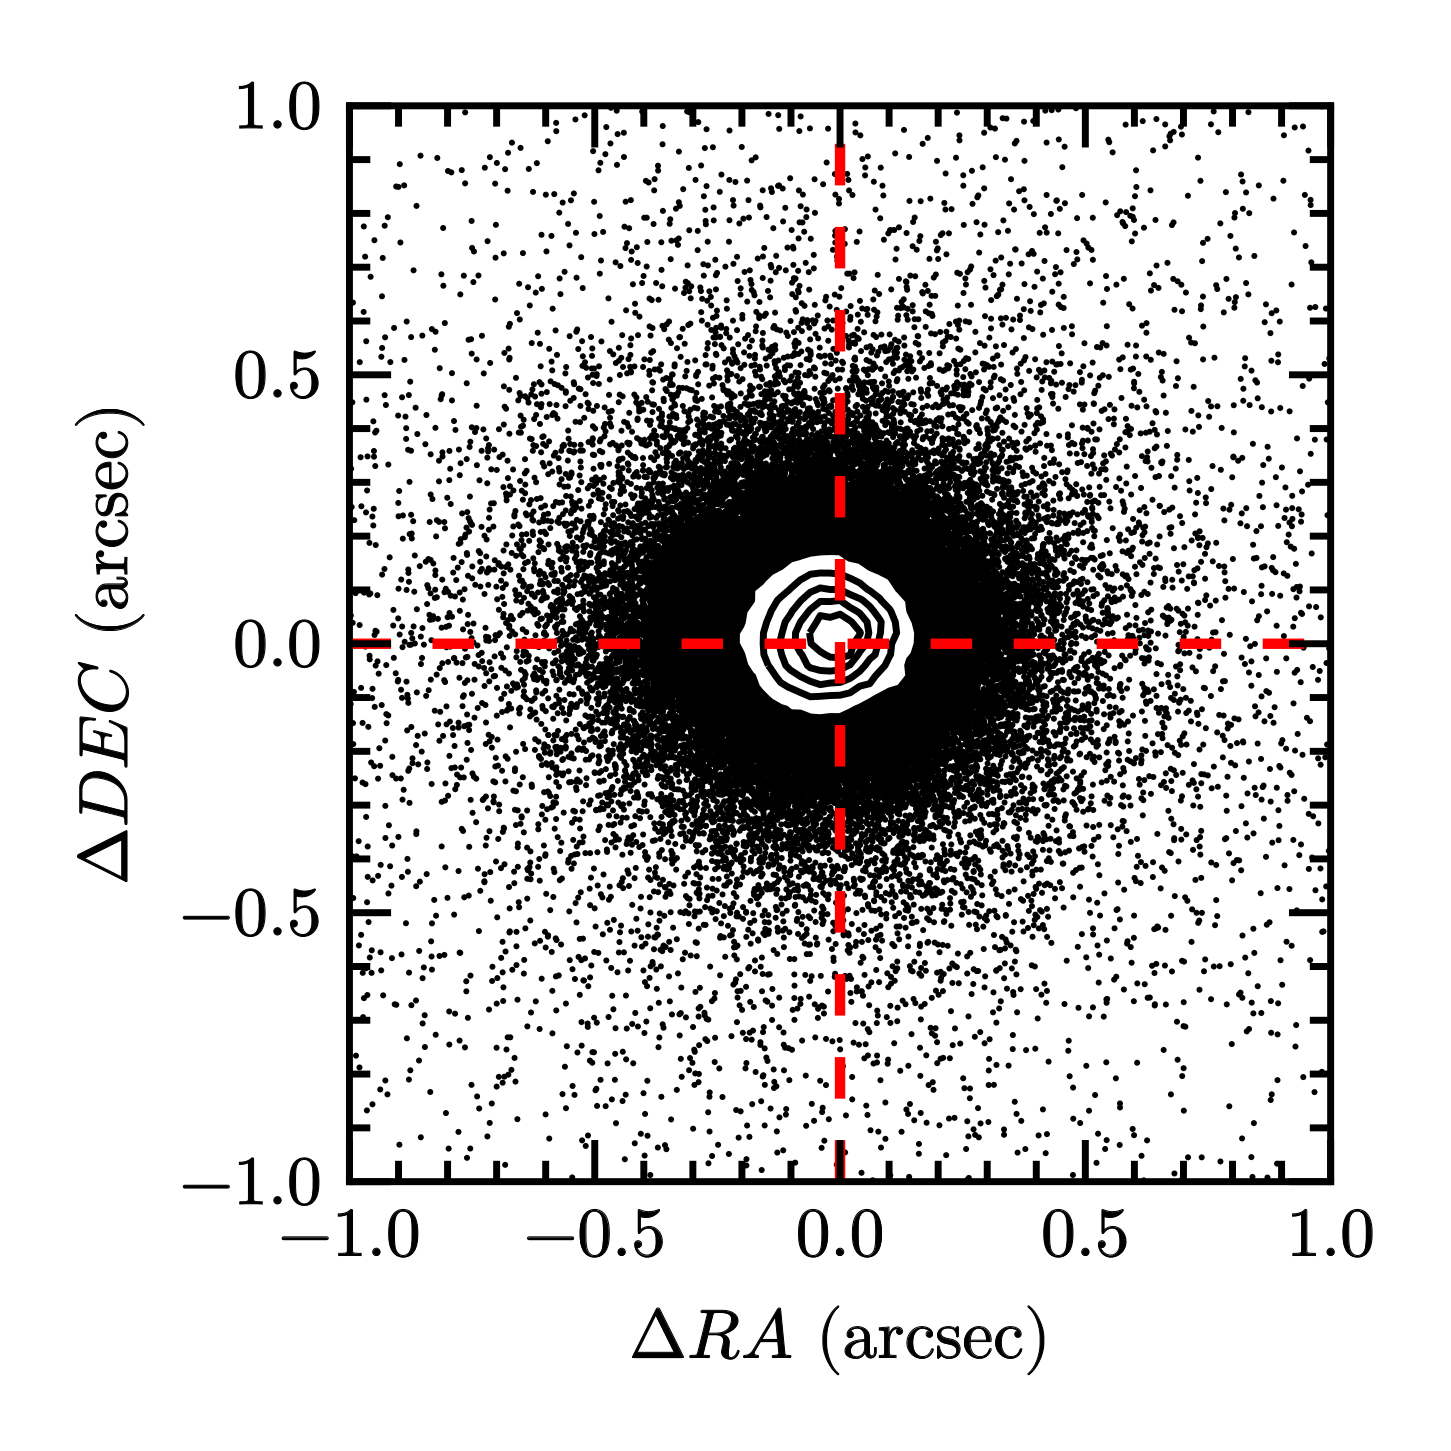
\includegraphics[width=0.5\textwidth]{astrometry_2d_separation.png}}
\subfloat[\label{fig:astrometry_sep}]{
	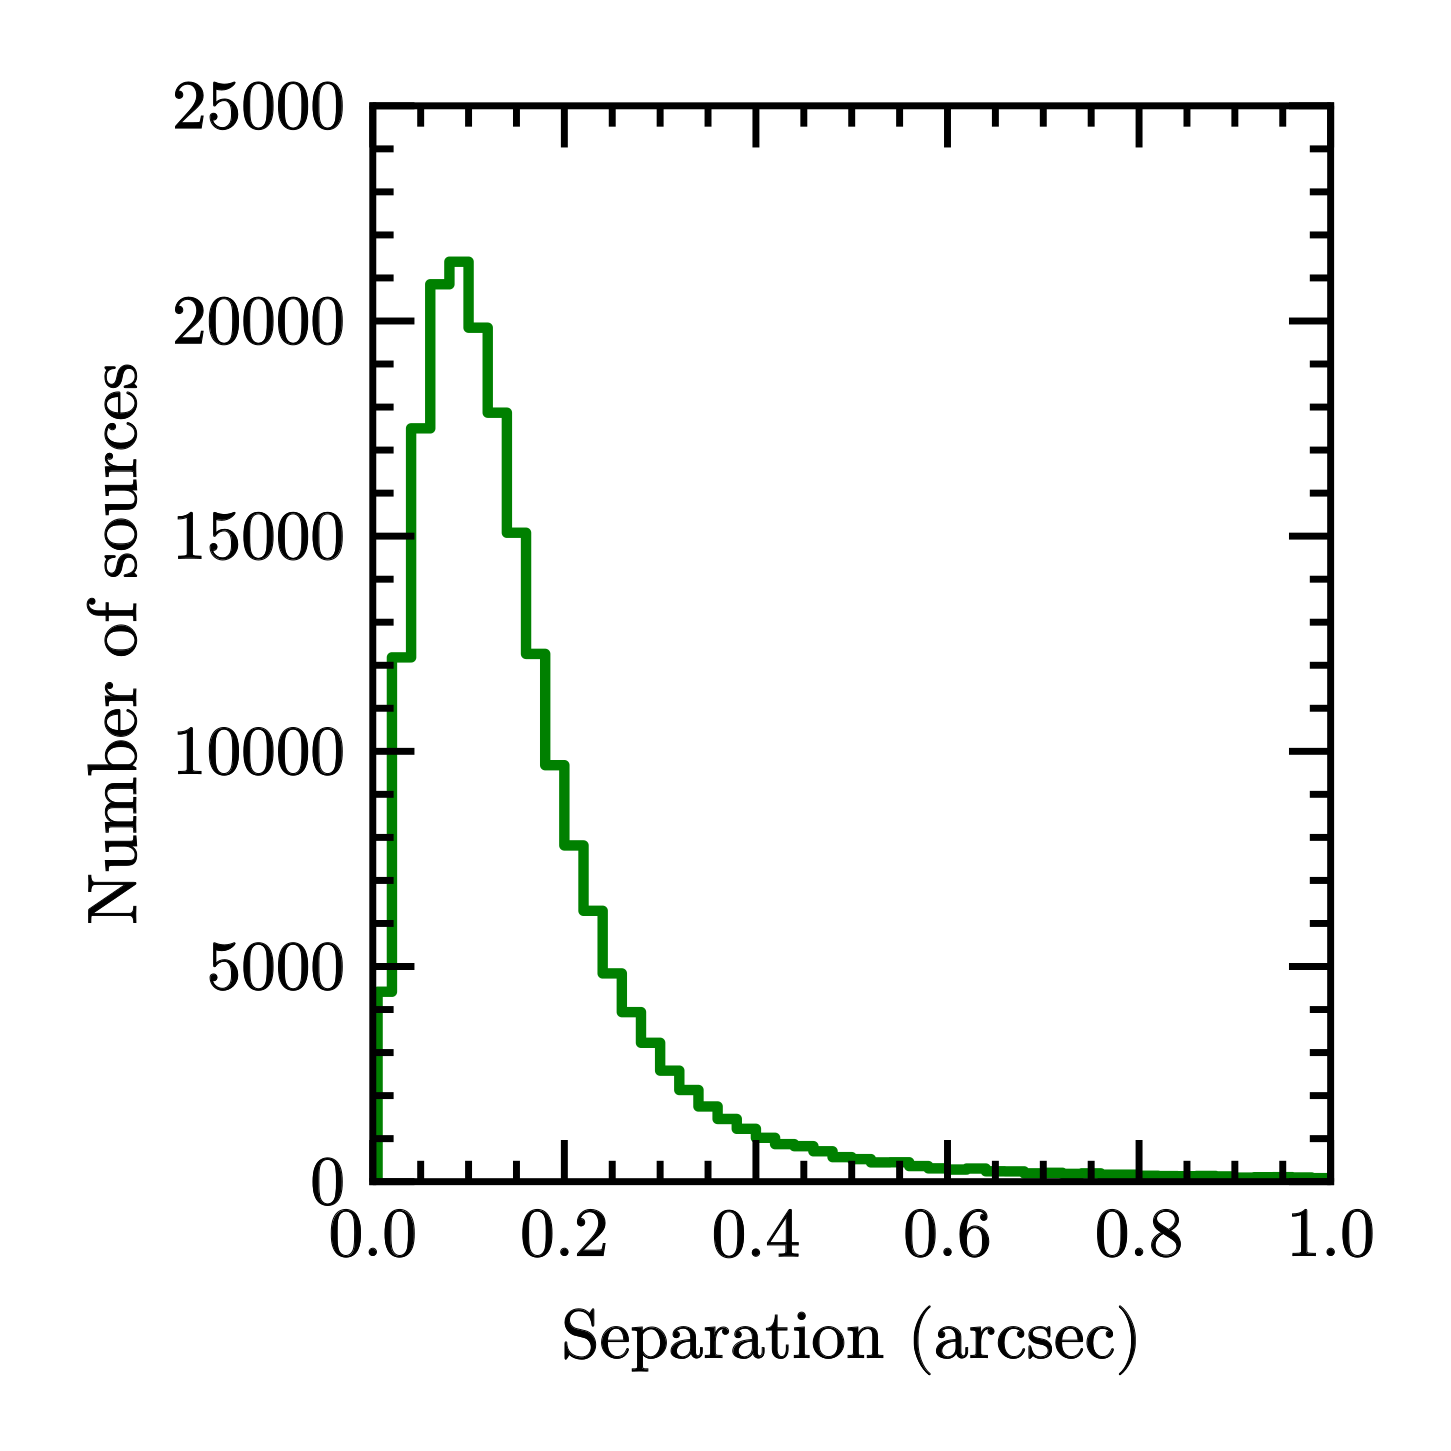
\includegraphics[width=0.5\textwidth]{astrometry_separation.png}}
\caption[Verification of the astrometry]{Comparison between DES and VIDEO astrometry for the \num{199 252} brightest non-duplicate objects, selected by imposing an SLR-corrected magnitude of $z_{\mathrm{DES,AB}}<22.0$. \textbf{(a)} Distribution of the difference  $\Delta RA$ and $\Delta DEC$ between the two surveys as defined in Equations \ref{eqn:ra_offset} and \ref{eqn:dec_offset}. The dashed red lines correspond to an offset of 0. \textbf{(b)} Histogram of the total separation $\Delta=\sqrt{{\Delta RA}^2 + {\Delta DEC}^2}$. Both (a) and (b) indicate excellent astrometric agreement.}
\label{fig:astrometry}
\end{figure*}





\subsection{Photometry verification}
The next validation test compares the photometry between the \DESVIDEO and \cite{2013MNRAS.428.1281J} VIDEO catalogues. For this test, the non-duplicate \DESVIDEO detections were again matched to the \cite{2013MNRAS.428.1281J} objects within a \SI{1}{\arcsec} radius. The magnitude offset between the two surveys was then computed for all matched detections, using magnitudes measured in a $\approx \SI{2}{\arcsec}$ diameter aperture (note: the two catalogues differ slightly in the aperture sizes that have been used  --- \SI{1.95}{\arcsec} for \DESVIDEO and \SI{2}{\arcsec} for \citealt{2013MNRAS.428.1281J}). Figure \ref{fig:mag_comparison} shows the resulting magnitude differences for each VIDEO filter as a function of magnitude. With mean offsets of < \SI{0.022}{\magab} in all filters, the two catalogues are generally in agreement, especially when considering that the \cite{2013MNRAS.428.1281J} apertures are slightly larger.  Despite this broad agreement, one may nevertheless note a slight bias towards bigger mean offsets (i.e. brighter \citealt{2013MNRAS.428.1281J} magnitudes) for redder filters, ranging from 0.007 for the $Z$-band to 0.022 in the $K_{s}$-band. There are several possible explanations for this trend. Firstly, the difference in aperture sizes may play a role. Even though the mean VIDEO PSF actually has a larger FWHM at shorter wavelengths (see Section \ref{subsubsection:data_quality_video}), it is possible that it has more extended wings at longer wavelengths, so that the (smaller) \DESVIDEO aperture catches less of the total flux in the redder filters. Secondly, the \DESVIDEO apertures for a given object have been placed in the same position for all bands (based on the $r+i+z$ detection image), whereas the positions in the \cite{2013MNRAS.428.1281J} catalogues have been derived from the morphology of the object in the reddest detected band (see Section \ref{subsubsection:video_data_reduction}).  For extended sources, this morphology can differ between filters if some regions of a galaxy contain bluer emission than others. Therefore, it is possible that for these sorts of objects the \DESVIDEO apertures are less optimally positioned, so that the \DESVIDEO measurements miss some red flux that is included in the \cite{2013MNRAS.428.1281J} catalogues. Nevertheless, the fact that even in the $K_{s}$-band the mean offsets are no larger than \SI{0.022}{\magab} demonstrates that the general agreement is good. This warrants a good degree of confidence in the accuracy of the \DESVIDEO photometry. \par

% \begin{figure}
% \centering
% \subfloat[\label{}]{
% 	\includegraphics[clip, width=0.50\textwidth]{mag_comparison_Z.png}}
% \subfloat[\label{}]{
% 	\includegraphics[clip, width=0.50\textwidth]{mag_comparison_Y.png}}

% \subfloat[\label{}]{
% 	\includegraphics[clip, width=0.50\textwidth]{mag_comparison_J.png}}
% \subfloat[\label{}]{
% 	\includegraphics[clip, width=0.50\textwidth]{mag_comparison_H.png}}

% \subfloat[\label{}]{
% 	\includegraphics[clip, width=0.50\textwidth]{mag_comparison_K.png}}	

% \caption[Verification of the photometry]{Comparison between VIDEO magnitudes from \DESVIDEO ($m_{\mathrm{DES+VIDEO}}$) and \cite{2013MNRAS.428.1281J} ($m_{\mathrm{VIDEO}}$), for all objects detected in both datasets. The grey dots show the magnitude difference $m_{\mathrm{DES+VIDEO}}-m_{\mathrm{VIDEO}}$ of each source as a function of \DESVIDEO magnitude. The black squares indicate the mean difference in bins of \SI{0.5}{\mag}. The coloured horizontal lines show the total mean value averaged over all grey data points, which is also listed in the legend. It must be noted that \DESVIDEO values have been measured in a \SI{1.95}{\arcsec} diameter aperture, as opposed to \SI{2}{\arcsec} for \cite{2013MNRAS.428.1281J}.}
% \label{fig:mag_comparison}
% \end{figure}

\begin{figure}[ph] 
\centering    
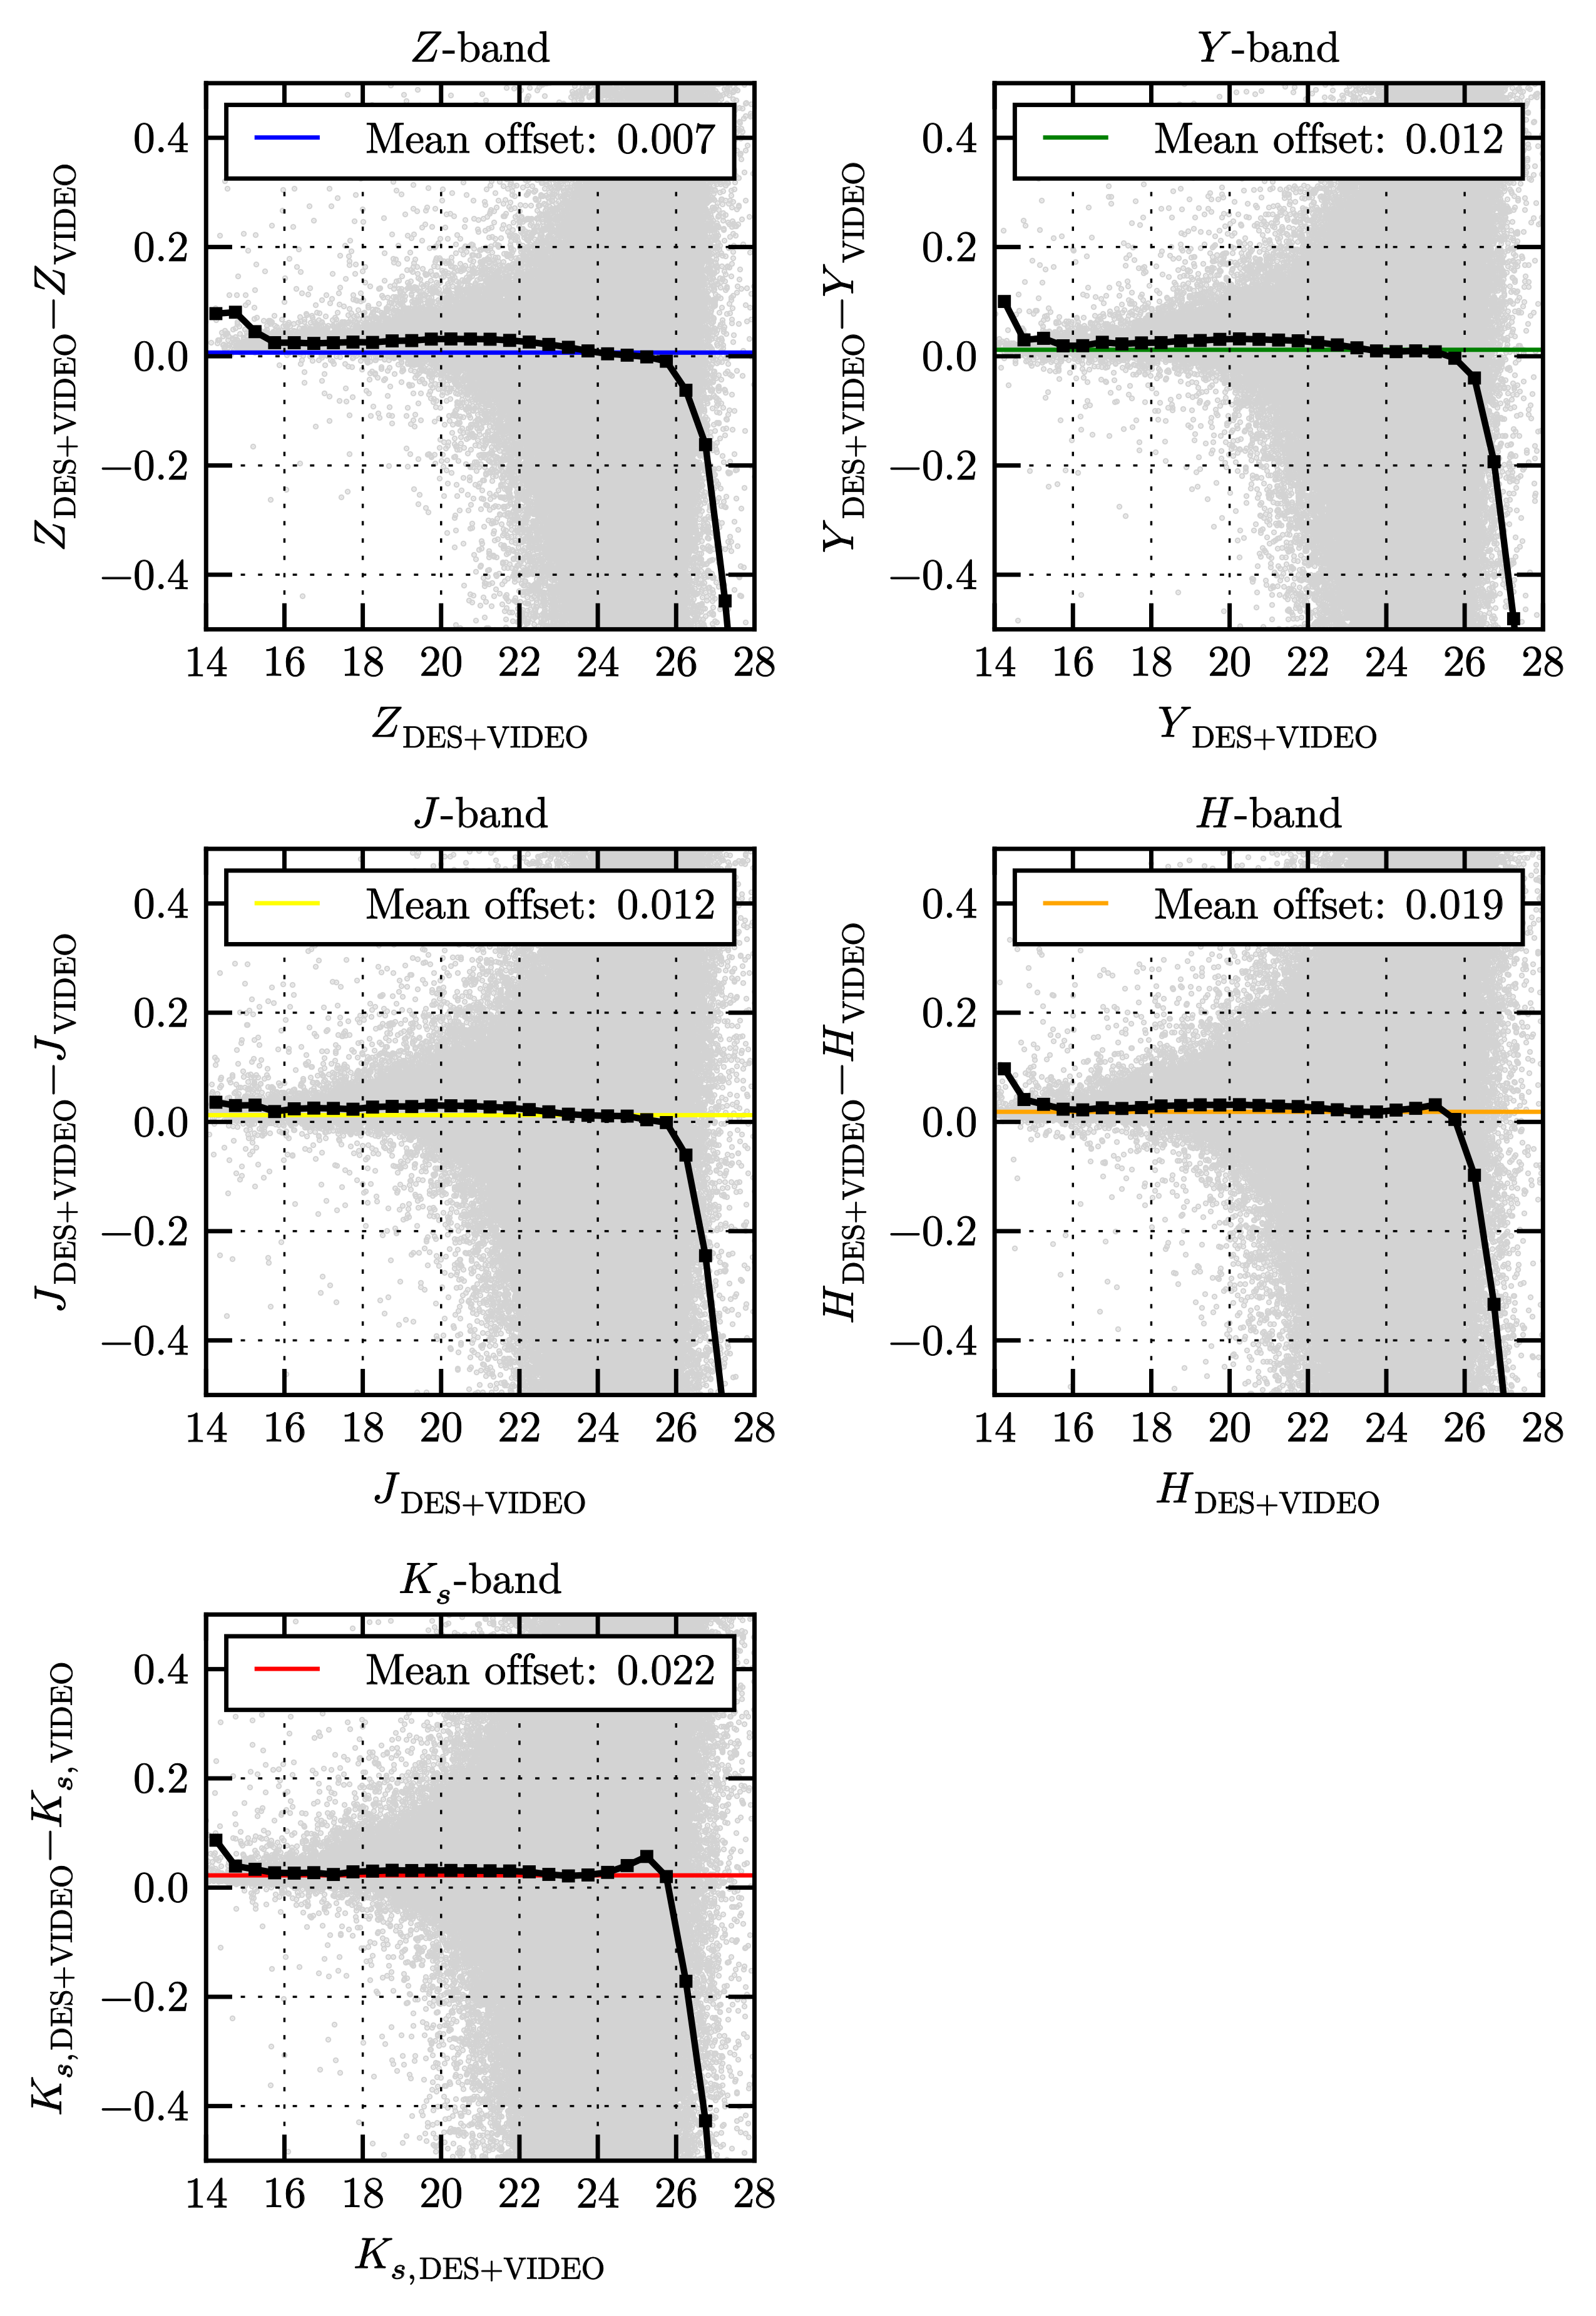
\includegraphics[width=0.95\textwidth]{mag_comparison.png}
\caption[Verification of the photometry]{Comparison between VIDEO magnitudes from \DESVIDEO ($m_{\mathrm{DES+VIDEO}}$) and \cite{2013MNRAS.428.1281J} ($m_{\mathrm{VIDEO}}$), for all objects detected in both datasets. The grey dots show the magnitude difference $m_{\mathrm{DES+VIDEO}}-m_{\mathrm{VIDEO}}$ of each source as a function of \DESVIDEO magnitude. The black squares indicate the mean difference in bins of \SI{0.5}{\mag}. The coloured horizontal lines show the total mean value averaged over all grey data points, which is also listed in the legend. It must be noted that \DESVIDEO values have been measured in a \SI{1.95}{\arcsec} diameter aperture, as opposed to \SI{2}{\arcsec} for \cite{2013MNRAS.428.1281J}.}
\label{fig:mag_comparison}
\end{figure}

 
 
\subsection{Forced photometry verification and results}\label{subsection:forced_phot_verification}
To assess the merits of the \DESVIDEO forced photometry strategy, the current section investigates whether the \DESVIDEO method indeed retrieves measurements for a larger number of sources than  \cite{2013MNRAS.428.1281J}. For this analysis, the \DESVIDEO source counts are compared to the number that would have been obtained via simple catalogue matching between the DESDM and \cite{2013MNRAS.428.1281J} catalogues. In order to estimate the latter number, the author assembled a position-matched dataset via the same catalogue assembly procedure as before (applying step 1, 3, 4, 6, and 8 from the algorithm presented in Section \ref{subsection:catalog_production}), this time using the \cite{2013MNRAS.428.1281J} catalogues instead of \DESVIDEO forced photometry in step 4. Including duplicates\footnote{The new matched catalogue contains duplicates, originating from the same tile overlap pattern that exists in the \DESVIDEO catalogue. A non-duplicate version was also produced.}, position matching retrieved \num{1 862 154} objects, which is 24\% less than the \num{2 443 576} sources obtained before via forced photometry. The unique (i.e. non-duplicate) total equals \num{1 676 054} with the \cite{2013MNRAS.428.1281J} catalogues, a 22\% decrease compared to the \num{2 152 575} unique sources in the forced photometry dataset. These two figures indicate that \DESVIDEO forced photometry indeed significantly increases the amount of information extracted from the VIDEO survey. Even more gains were made in those regions where DES imaging is significantly deeper than VIDEO. For example, in the cdfs1 tile, forced photometry retrieves fluxes for \num{393616} objects (including duplicates), compared to \num{257812} from matching to \cite{2013MNRAS.428.1281J} ---  an improvement of $\approx 35\%$. Without duplicates, these numbers are \num{376079} vs \num{246755}, implying an increase of $\approx 34\%$. \par


\begin{figure*}[tpb]
\centering
\subfloat[\label{fig:number_counts_Ks_total}]{
	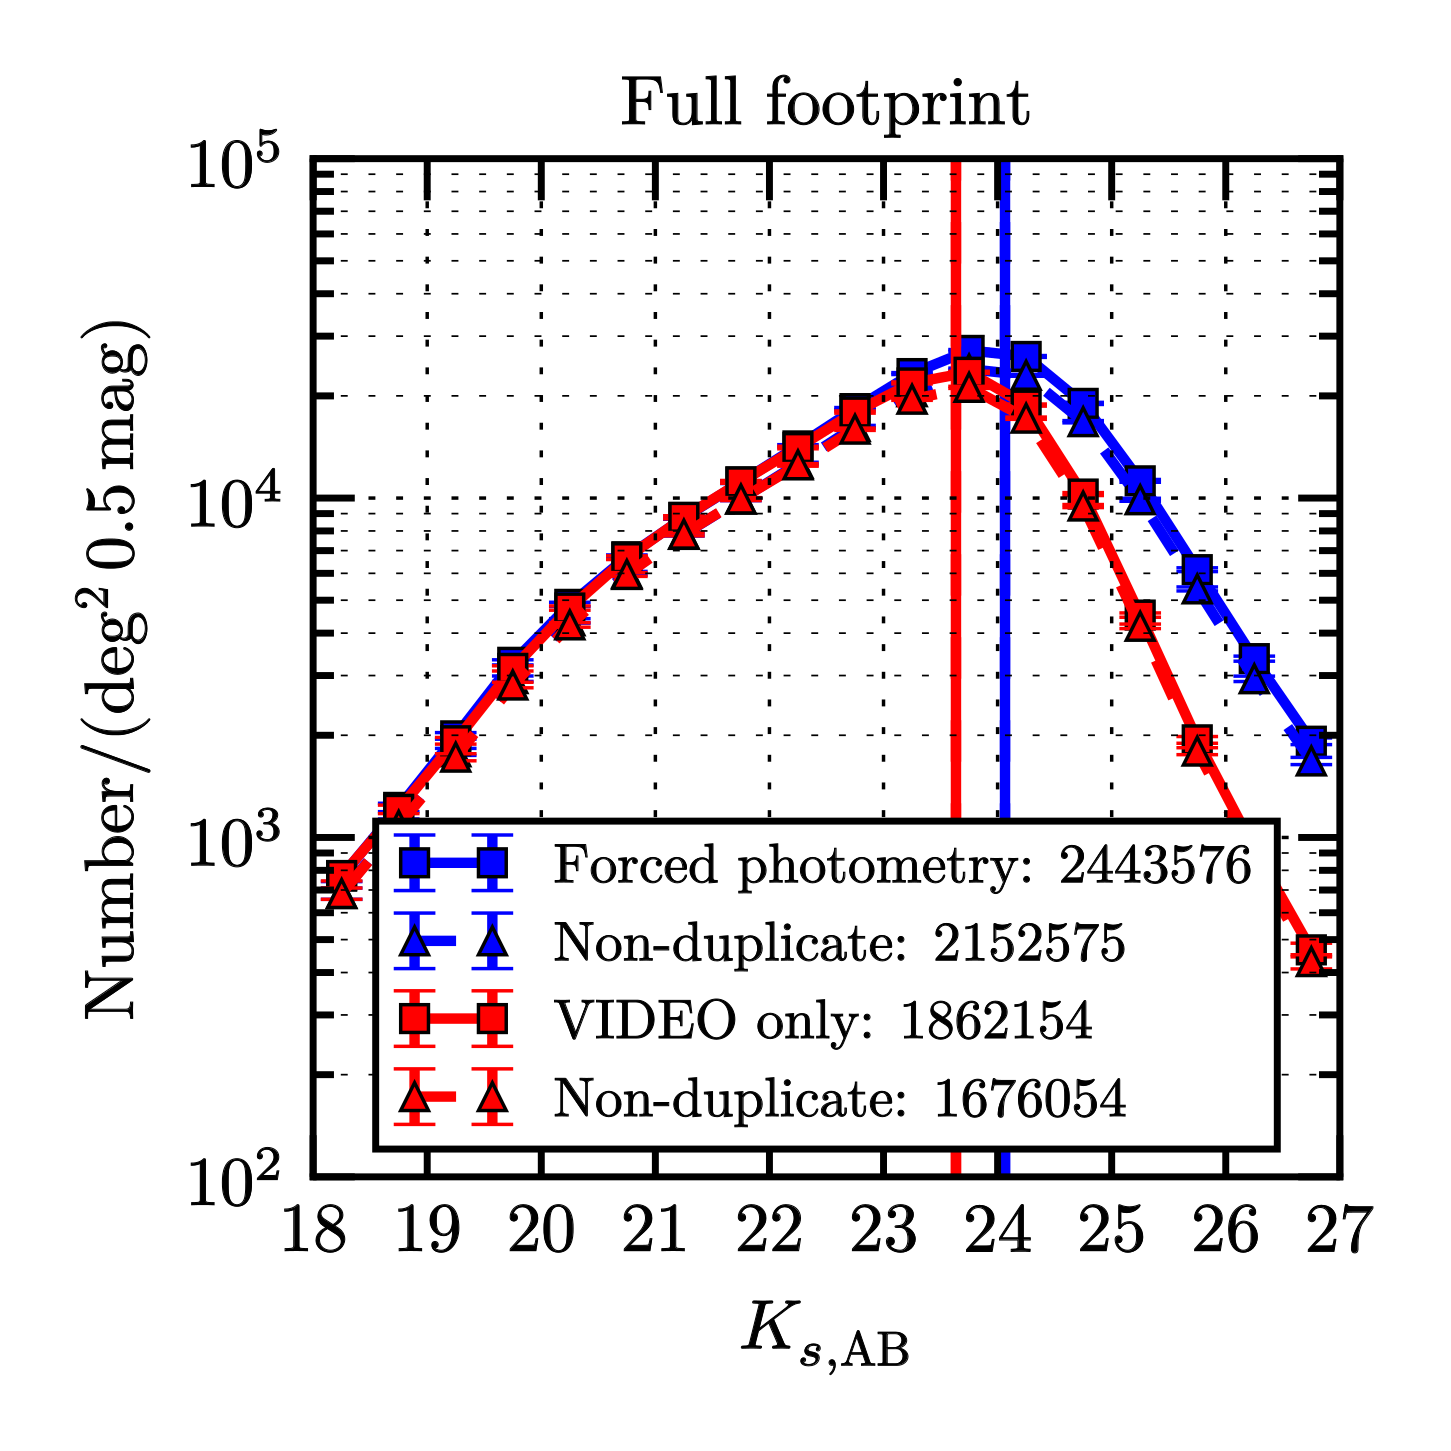
\includegraphics[clip, width=0.50\textwidth]{Chapter2/Figs/number_counts_Ks.png}}
\subfloat[\label{fig:number_counts_Ks_cdfs1}]{
	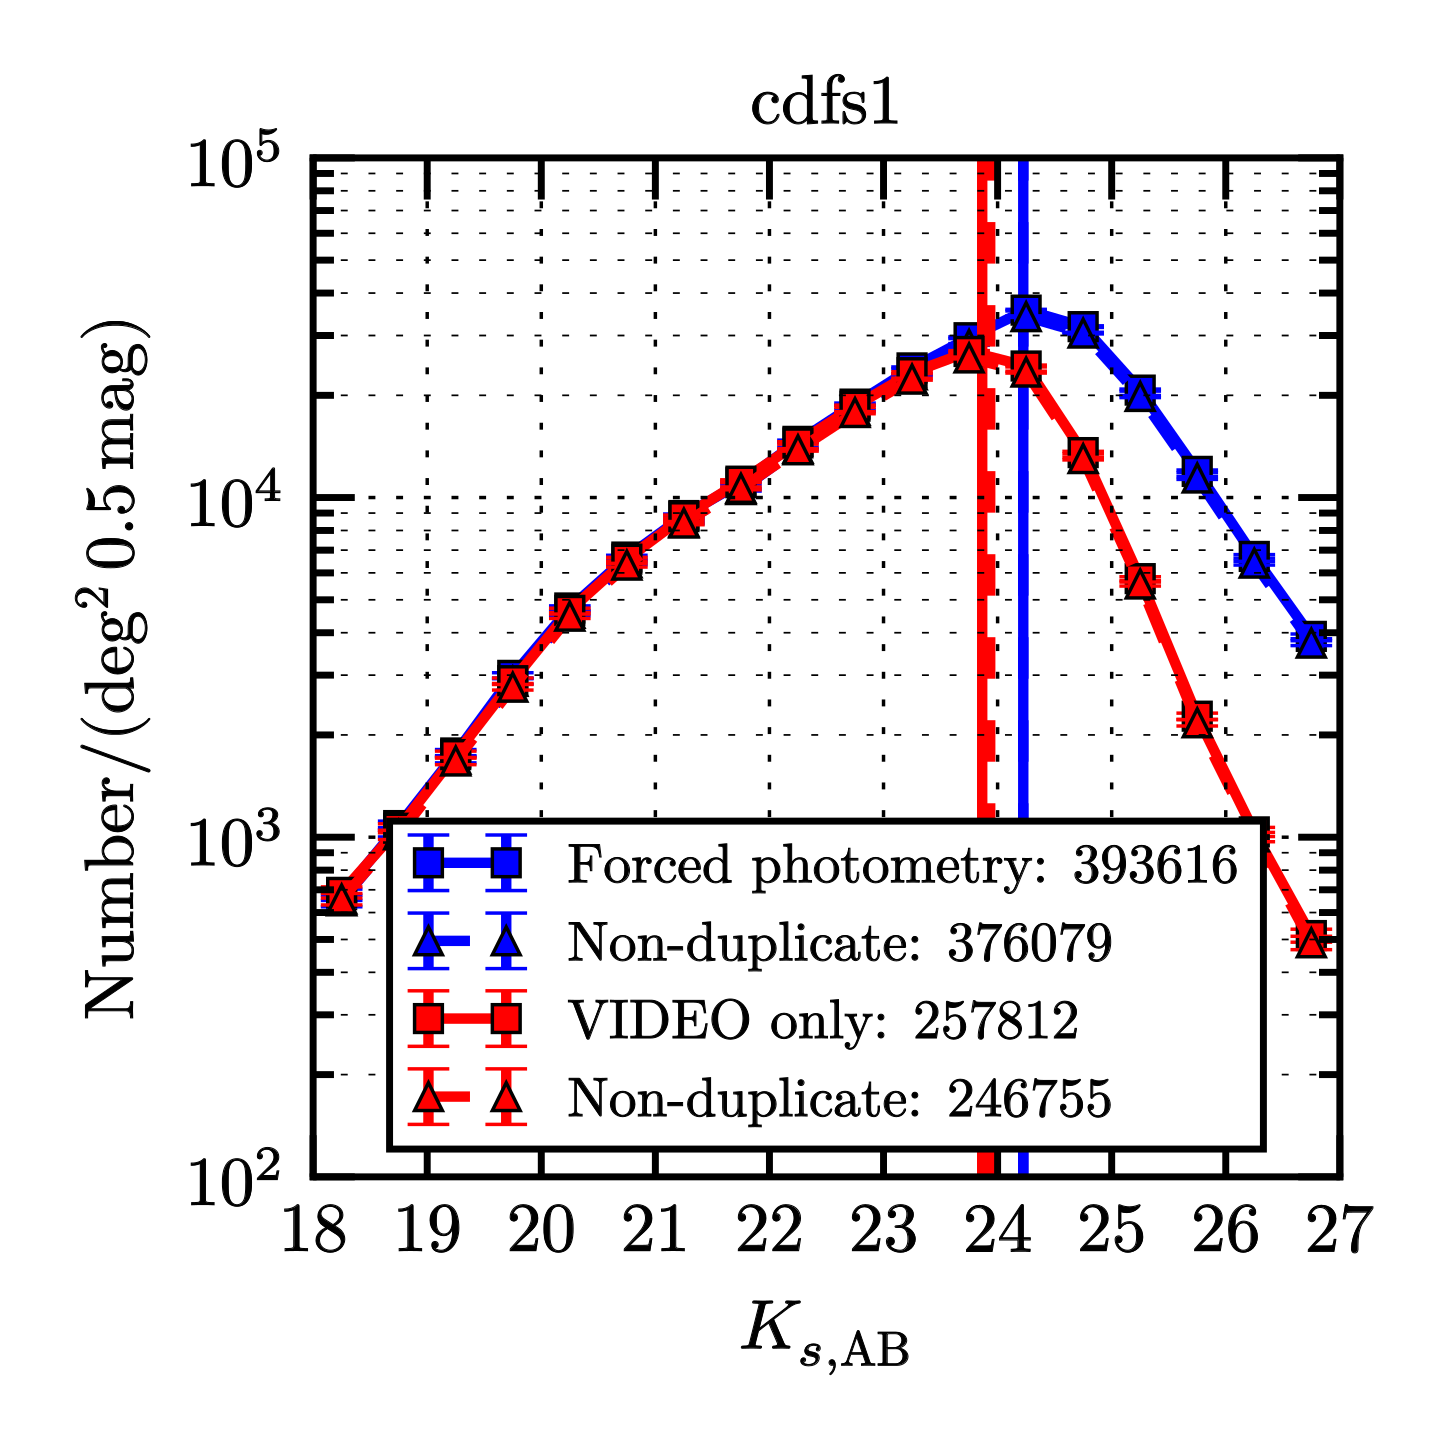
\includegraphics[clip,width=0.50\textwidth]{Chapter2/Figs/number_counts_Ks_cdfs1.png}}
\caption[Number counts in the \texorpdfstring{$K_{s}$}{}-band]{ Number counts per \si{\sqdeg} as a function of $K_{s}$-band magnitude, in bins of \SI{0.5}{\mag}. \DESVIDEO forced photometry (measured in \SI{1.95}{\arcsec} apertures) outcomes are shown in blue. The outcomes from position matching to the \cite{2013MNRAS.428.1281J} VIDEO catalogues (measured in \SI{2}{\arcsec} apertures) are shown in red. Solid lines with squares denote results including duplicates, and the dashed lines and triangles denote results after duplicates have been removed. All data points contain error bars corresponding to Poisson counting uncertainties, but these are smaller than the symbol size in almost all cases. Maxima for all distributions are computed in smaller \SI{0.01}{\mag} bins and denoted by vertical lines. \textbf{(a)} Results for the full \DESVIDEO footprint. The \DESVIDEO maxima both lie at $K_{s,\mathrm{AB}} = 24.065$ (with and without duplicates), and the \cite{2013MNRAS.428.1281J} maxima are at $K_{s,\mathrm{AB}} = 23.635$ (idem). \textbf{(b)} Results for the cdfs1 tile only. The \DESVIDEO maxima lie at $K_{s,\mathrm{AB}} = 24.225$ (with and without duplicates), and the \cite{2013MNRAS.428.1281J} maxima are at $K_{s,\mathrm{AB}} = 23.865$ with duplicates and at $K_{s,\mathrm{AB}} = 23.935$ without duplicates.}
\label{fig:number_counts_Ks}
\end{figure*} 

Further analysis of the number counts also shows that \DESVIDEO forced photometry extracts data for fainter sources than is possible with VIDEO alone. Figure \ref{fig:number_counts_Ks_total}  illustrates this finding by plotting the number of \DESVIDEO vs matched \cite{2013MNRAS.428.1281J} objects as a function of $K_{s}$-band magnitude, per \si{\sqdeg} in bins of \SI{0.5}{\mag}. Like in the previous section, these magnitudes are measured in a $\approx\SI{2}{\arcsec}$ diameter aperture (\SI{1.95}{\arcsec} for \DESVIDEO and \SI{2}{\arcsec} for \citealt{2013MNRAS.428.1281J}). Importantly, the \DESVIDEO number counts agree well with the \cite{2013MNRAS.428.1281J} results at the bright end, but come out considerably higher at the faint end as the \cite{2013MNRAS.428.1281J} distribution starts to roll over. This is exactly the behaviour that one would expect if \DESVIDEO forced photometry indeed extracts data from objects that are too faint to be detected reliably in VIDEO alone. To quantify this increase in faint source counts, the maximum of the $K_{s}$ distribution was determined for both catalogues (grouping magnitudes in smaller bins of \SI{0.01}{\mag} for increased resolution). Without forced photometry, this peak\footnote{All the maxima in this paragraph are given without duplicates, the results including duplicates are shown in Figure \ref{fig:number_counts_Ks} for completeness.} lies at $K_{s,\mathrm{AB}} = 23.635$, whereas the \DESVIDEO peak occurs at $K_{s,\mathrm{AB}} = 24.065$. This indicates that the \DESVIDEO method pushes the VIDEO measurements $\approx \SI{0.4}{\mag}$ fainter (possibly even a bit more given the fact that the \DESVIDEO apertures are slightly smaller than those from \citealt{2013MNRAS.428.1281J}). The above analysis was repeated for the cdfs1 tile studied in the previous paragraph. These results are plotted in Figure \ref{fig:number_counts_Ks_cdfs1}. Here, the \cite{2013MNRAS.428.1281J} maximum occurs at $K_{s,\mathrm{AB}} = 23.935$, while the \DESVIDEO distribution peaks at $K_{s,\mathrm{AB}}=24.225$, i.e. $\approx \SI{0.3}{\mag}$ fainter. This is slightly less than the $\approx \SI{0.4}{\mag}$ increase for the full footprint, most likely due to the fact that the $K_{s}$ data in this tile is slightly deeper than average (see Table \ref{table:error_agreement}). Because \cite{2013MNRAS.428.1281J} based their source detections on the reddest filter in which a given object is detected  (which is often the $K_{s}$-band), in this tile their detection strategy performs slightly above average. Therefore, the  \DESVIDEO forced photometry provides a comparatively smaller increase in faint $K_{s}$-observed sources. One may recall from the previous paragraph that forced photometry does, however, perform above average in the cdfs1 tile in terms of overall source counts (when compared to the full footprint).  This can be attributed to the fact that the $Z$-band imaging is shallower than average in this tile, which means that the corresponding \cite{2013MNRAS.428.1281J} catalogue contains fewer `blue' objects that are undetectable in $YJHK_{s}$ but would nevertheless show up in deeper $Z$-band imaging. At the same time, the DES $z$-band is much deeper than VIDEO in this region, so the \DESVIDEO pipeline does manage to retrieve these blue objects. \par 

The fact that forced photometry can be used to obtain photometry for more and for fainter objects has been shown several times before (e.g. \citealt{2015MNRAS.446.2523B,2016AJ....151...36L,2017ApJS..230....9N}). In fact, the very similar study by \cite{2015MNRAS.446.2523B} demonstrated this principle for the DES wide-field (detection) and VHS (measurement) data. Exploiting the fact that their DES data is considerably deeper than VHS ($\sim\SI{4}{\magab}$ when comparing $i$- and $J$-band magnitudes), they found that forced photometry increases the number of objects with measured VHS fluxes by a factor of 4.5 and pushes the VHS 80\% completeness limit \SI{1.5}{\mag} deeper. Comparatively, the 1.22 times increase in numbers and  \SI{0.4}{\mag} increase in depth found by this thesis are not quite as enormous, since the DES deep field and VIDEO surveys are more evenly matched in terms of limiting magnitudes ($<\SI{2}{\magab}$ difference between $i$ and $J$). However, the \DESVIDEO results nevertheless add to the existing body of evidence in favour of using forced photometry to combine surveys. On top of that, they also demonstrate that doing so can lead to considerable gains even if one survey is only moderately deeper than the other. \par


\begin{figure*}[tpb]
\centering
\subfloat[]{
	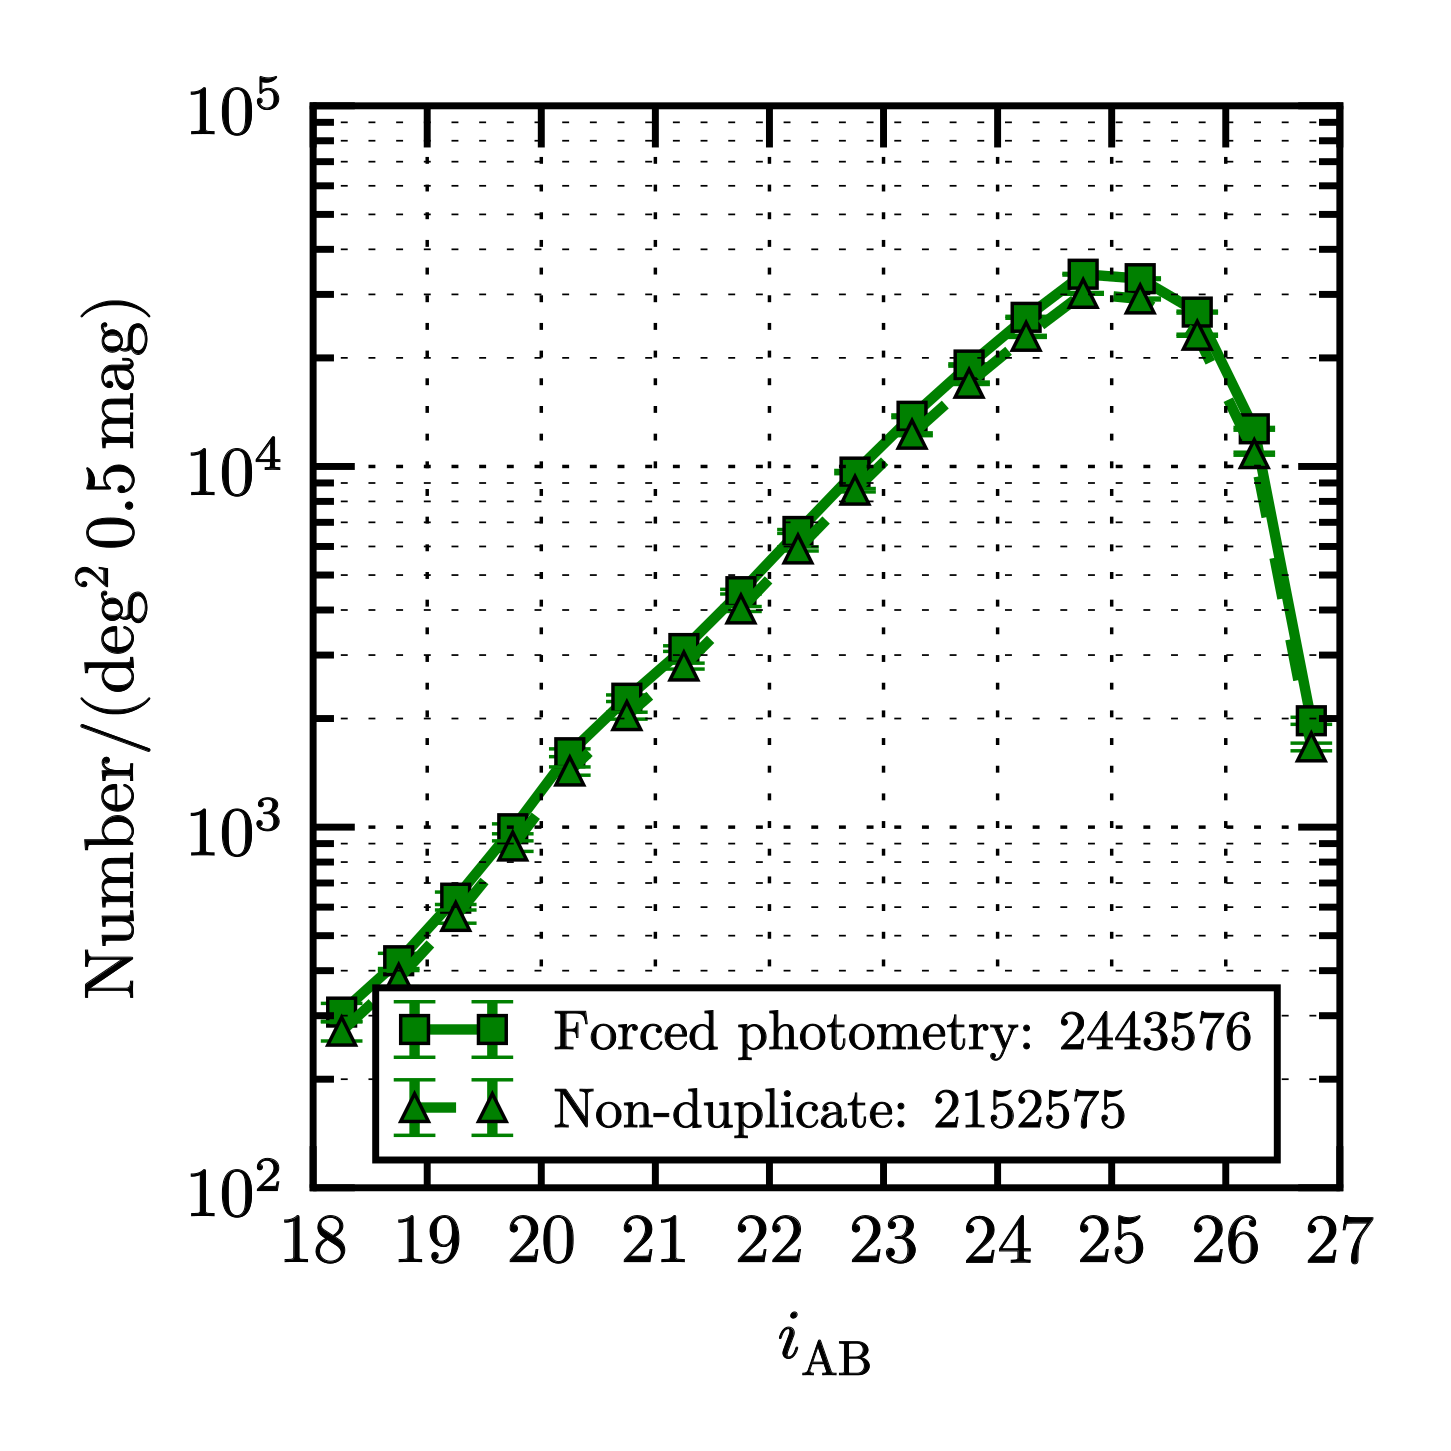
\includegraphics[clip, width=0.50\textwidth]{Chapter2/Figs/number_counts_i.png}}
\subfloat[]{
	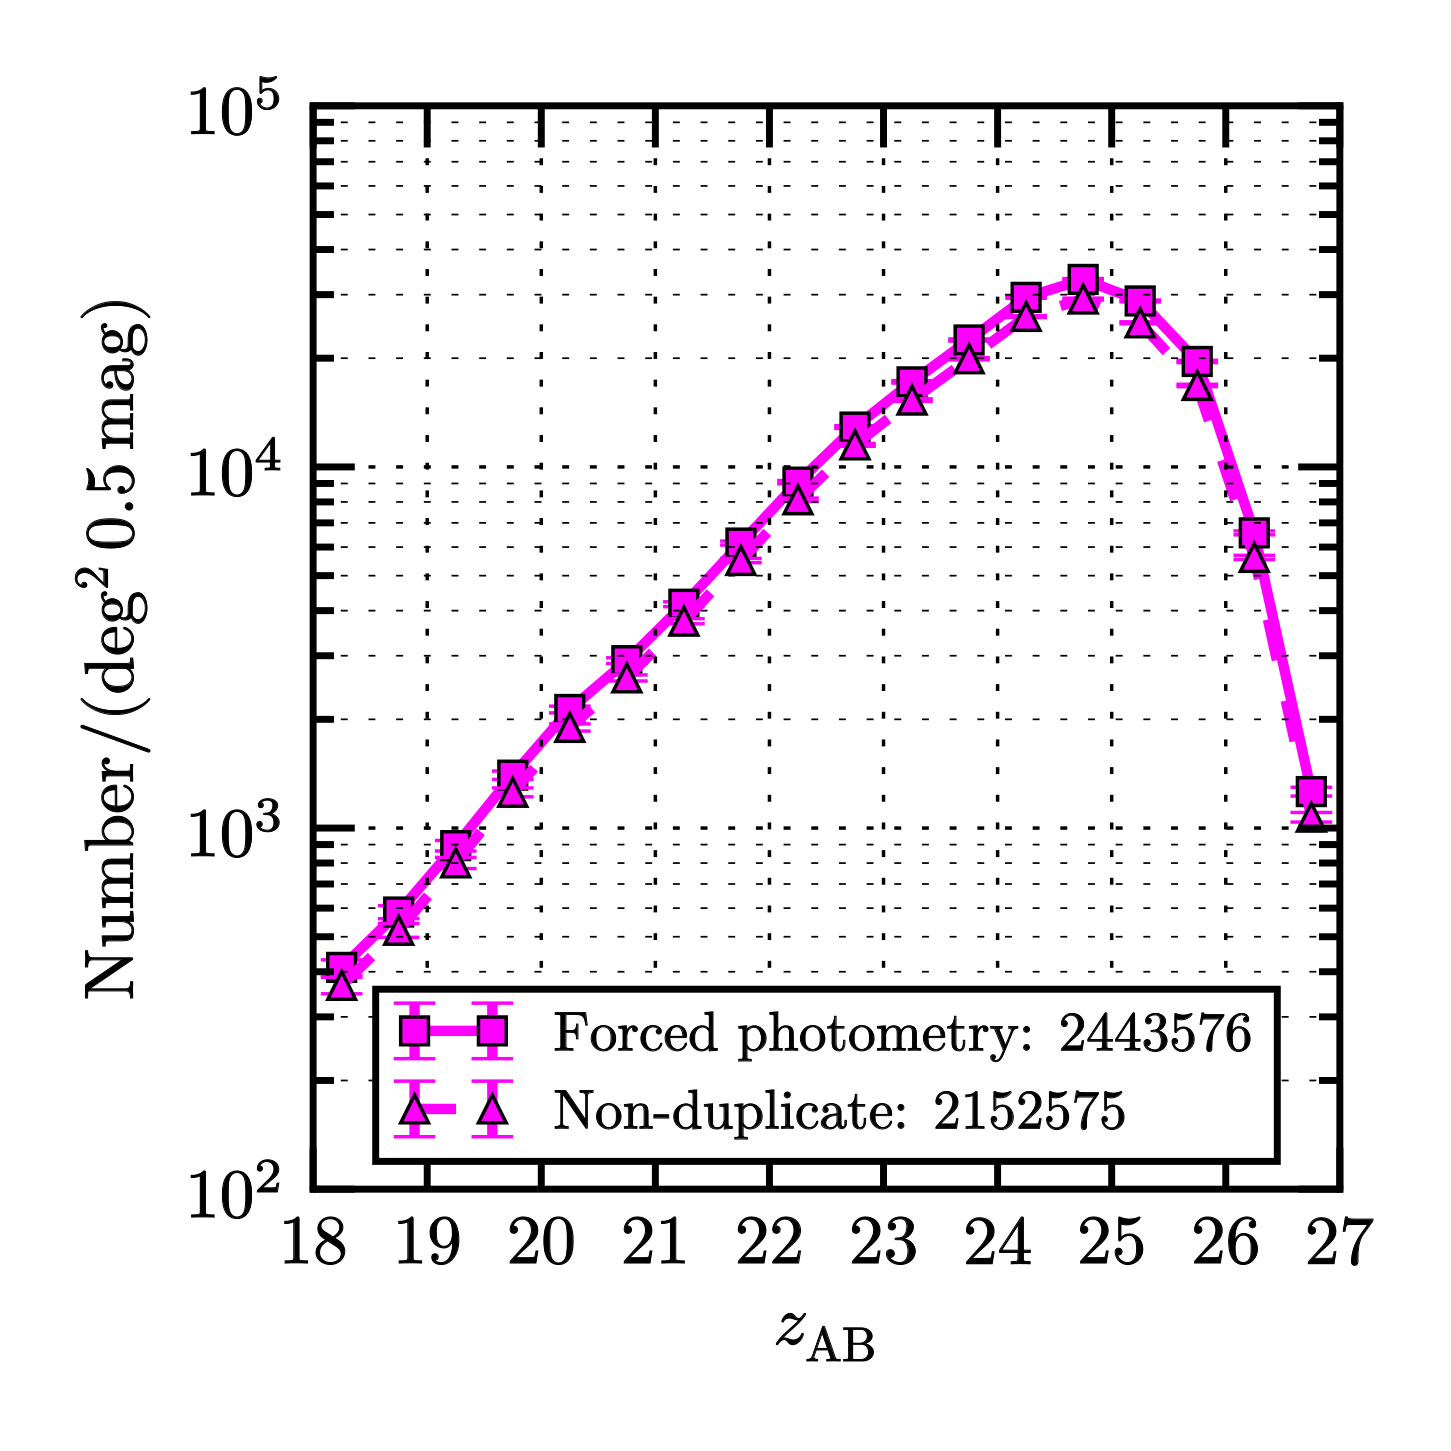
\includegraphics[clip, width=0.50\textwidth]{Chapter2/Figs/number_counts_z.png}}
\caption[Number counts in the \texorpdfstring{$i$}{}-band and \texorpdfstring{$z$}{}-band]{Number counts for the \DESVIDEO catalogue per \si{\sqdeg} as a function of \SI{1.95}{\arcsec} magnitudes in bins of \SI{0.5}{\mag}. The solid lines with squares show results including duplicates, and the dashed lines and triangles show results after duplicates have been removed. Data points for each bin include error bars corresponding to uncertainties from Poisson counting, but these are smaller than the symbol size in almost all cases. \textbf{(a)} Results for the DES $i$-band. \textbf{(b)} Results for the DES $z$-band.}
\label{fig:number_counts_DES}
\end{figure*}


\subsection{Catalogue results}
The validation tests above confirm that the astrometry and photometry of the \DESVIDEO catalogue are indeed accurate, and that the forced photometry is functioning as intended. This establishes the catalogue as a suitable general resource for the scientific community, and demonstrates that it can provide a solid backbone for the photometric redshifts and high-redshift galaxy search later in this thesis. \par 

%The \DESVIDEO catalogue can thus provide a solid backbone for the photometric redshifts and high-redshift galaxy search later in this thesis. 

For the sake of  providing a comprehensive overview of the full catalogue, Figure \ref{fig:number_counts_DES} shows the \DESVIDEO number counts in the $i$-band and $z$-band as a function of magnitude. The distributions behave as expected from the area-depth distributions in Figure \ref{fig:area_depth}. The $z$-band distribution peaks roughly $z_{\mathrm{AB}}\approx24.75$, which approximately corresponds to the $z_{5\sigma}\geq24.9$ magnitude limit for the largest \SI{10.8}{\sqdeg} section of the total footprint. The number counts then decline slightly with increasing magnitude, falling sharply after $z_{\mathrm{AB}}\sim 25.75$. This turning point is reasonably close to the $z_{5\sigma}\geq26.2$ limiting magnitude of the deepest \SI{4.3}{\sqdeg}. Similarly, the maximum of the $i$-band distribution lies around $i_{\mathrm{AB}}\approx25.0$, in agreement with the limiting $i_{5\sigma}\geq25.1$ limiting magnitudes in the largest \SI{10.7}{\sqdeg} $i$-band area. The second turnover at $i_{\mathrm{AB}}\approx 26.0$ again lines up approximately with the $i_{\sigma}\geq26.3$ depths in the deepest \SI{4.4}{\sqdeg} $i$-band regions of the catalogue. \par 

%!TEX root = ../thesis.tex
%*******************************************************************************
%****************************** Third Chapter **********************************
%*******************************************************************************
%\newcommand*\diff{\mathop{}\!\mathrm{d}}
%\newcommand{\overbar}[1]{\mkern 1.5mu\overline{\mkern-1.5mu#1\mkern-1.5mu}\mkern 1.5mu}

%\newcommand*\diff{\mathop{}\!\mathrm{d}} 





\chapter{Photometric redshifts}\label{chapter:photometric_redshifts}

% **************************** Define Graphics Path **************************
\ifpdf
    \graphicspath{{Chapter3/Figs/Raster/}{Chapter3/Figs/PDF/}{Chapter3/Figs/}}
\else
    \graphicspath{{Chapter3/Figs/Vector/}{Chapter3/Figs/}}
\fi

\section{Motivation}\label{section:motivation}
%ADD MORE FLUFF
%INCREASE FOOTNOTE DIVIDER SPACE
%several hundred, possibly thousand

A key result of Chapter \ref{chapter:catalogue} has been the production of a \DESVIDEO source catalogue  that covers \SI{10.8}{\sqdeg} to depths of $z_{5\sigma}\geq25.0$ and a smaller sub-area of \SI{4.3}{\sqdeg} to $z_{5\sigma}\geq26.2$. At the time of writing, this dataset contains the largest footprint to comparable depths over optical and near-IR wavelengths. This makes the \DESVIDEO catalogue a highly attractive resource to search for the brightest ($m_{\mathrm{AB}}<25.0$) galaxies at $z\gtrsim5$. As explained in Section \ref{section:high_redshift_galaxies}, the study of galaxy evolution in the early universe would benefit greatly from the discovery of more of these rare sources, and finding extremely bright high-redshift galaxies is therefore one of the core aims of this thesis. Due to their rarity, no more than a few dozen of these objects are expected within the \DESVIDEO footprint (as will be argued later in Section \ref{subsubsection:expected_number}). This number is evidently small when compared to the catalogue total of \num{2 152 575} unique sources, which indicates that the search will require an efficient and clean selection method. Section \ref{subsection:high_z_selection_methods} described several effective methods that have been developed in the literature, of which Lyman-break colour selection and photometric redshifts are the most appropriate for the current dataset. Even though both strategies have historically been highly successful, this thesis  will opt for a photometric redshift approach. The main reason behind this choice is that for the purpose of selecting candidates, colour-colour methods only use the information from the three bands used in the colour cuts, whereas photometric redshifts incorporate data from all available wavelengths. Given that the \DESVIDEO catalogue covers the full optical+near-IR range in 10 filters of which 9 are deep enough for the photo-zs in this thesis, a photometric redshift approach makes better use of all the available information. Furthermore, as described in Section \ref{subsection:methods}, some photometric redshift methods offer sophisticated probabilistic data handling options, providing another edge over simple colour-cut methods. Features such as the inclusion of a redshift-luminosity prior (see Section \ref{subsection:prior}) or probability distribution (see Section \ref{subsubsection:chi_minimisation}), can be used to remove objects consistent with a low-redshift solution, in order to increase the purity of a high-redshift sample. \par


%The number of high redshift galaxies expected in the \DESVIDEO catalogue is evidently small when compared to the catalogue total of 2 284 987 objects, suggesting a need for an efficient and clean selection method.

In addition to the fact that photometric redshifts offer a more sophisticated treatment of the available flux information, they also deliver redshifts for all objects, instead of only selecting a particular high-redshift sample. This is an important asset for the \DESVIDEO catalogue. Given its utility as a general resource for the scientific community (as proposed in Sections \ref{subsection:conclusion_surveys_intro} and \ref{subsection:conclusion_photoz_intro}), equipping the \DESVIDEO catalogue with photometric redshifts for all \num{2443576} objects will be of general interest. Moreover, because \num{35596} sources have spectroscopic redshifts, their photo-zs can also be used for a case-study of photometric redshift performance. As explained in Sections \ref{subsubsection:photoz_applications_intro} and \ref{subsection:conclusion_photoz_intro}, because photometric redshifts play a crucial role in modern astronomy, such performance tests are highly important, and therefore form another aim of this thesis.\par


The task of calculating photometric redshifts for the \DESVIDEO catalogue is the topic of the current chapter. As part of that process, several photo-z options and features are tested in terms of their performance. At the end, the most suitable configuration is selected to calculate the final \DESVIDEO redshifts. As a concluding remark, it is helpful to emphasise the priorities that have informed some of the choices involved here. Despite the secondary goal of providing photometric redshifts for general use, it must be stressed that the final \DESVIDEO redshift catalogue is primarily created with the selection of $z\gtrsim5$ objects in mind. Thus, the tweaking of the photometric redshift code is aimed towards producing optimal results for high-redshift galaxies, possibly at the cost of fine accuracy for the bulk of the objects at $z\lesssim1.5$. This is a conscious choice, and anyone who wishes to use the photometric redshifts for low-redshift research must bear this caveat in mind.\par

%As a concluding remark, it is helpful to emphasise the priorities that informed some of the choices that will be made here. Despite the secondary goal of providing photometric redshifts for general use, it must be stressed that the \DESVIDEO redshift catalogue will be primarily created with the selection of $z\gtrsim5$ objects in mind. Thus, the tweaking of the photometric redshift code will be aimed towards producing optimal results for high-redshift galaxies, possibly at the cost of {\color{red} fine} accuracy for the bulk of the objects at $z\lesssim2$. This is a conscious choice, and anyone who wishes to use the photometric redshifts for low-redshift research must bear this caveat in mind. 



\section{Description and implementation of the photometric redshift algorithm}\label{section:LePHARE}
\subsection{Choice of code}\label{subsection:code_choice}
With a strong case established in favour of calculating photometric redshifts for the \DESVIDEO dataset, the next step involves selecting a particular code from the large suite of publically available codes described in 
Section \ref{subsection:methods}. To recap briefly, these codes can be grouped into two categories: template fitting methods and empirical methods. Empirical methods rely on spectroscopic redshifts to calibrate an observed colour-redshift relationship empirically, and therefore require a large and representative set of spectroscopic redshifts to function. There is evidence that empirical codes outperform template fitting methods when such a set is available \citep{2011MNRAS.417.1891A,2019NatAs...3..212S}, and that template codes are more suited to regimes where this is not the case, such as at high redshift \citep{2019NatAs...3..212S}. As demonstrated in Section \ref{subsection:spectra}, the spectroscopic coverage in the \DESVIDEO catalogue is sparse at high redshifts, with only 11 objects at $z_{\mathrm{spec}}>4.0$. Due to these extremely small numbers, empirical codes will not be reliable in this redshift range. Since optimal performance at $z\gtrsim5$ is the main priority of the photometric redshift catalogue, a template fitting code is deemed to be the most suitable option. \par


As described in Section \ref{subsubsection:intro_comparison}, studies in the literature comparing different codes have failed to produce a clear consensus on a single best template code \citep{2010A&A...523A..31H,2011MNRAS.417.1891A,2013ApJ...775...93D}. The choice of code for this thesis was therefore informed primarily by what extra features the different codes provide. It was decided to use \texttt{LePHARE} \citep{2006A&A...457..841I,2009ApJ...690.1236I}, predominantly on the basis that it offers a way to calibrate magnitude offsets within photometric bands (a detailed description of this feature and how it benefits the \DESVIDEO catalogue will be presented in Section \ref{subsection:adaptive_offsets}). The fully probabilistic Bayesian approach is also advantageous, especially because it permits the option to include a luminosity prior (see Section \ref{subsection:prior}), and can make use of a redshift probability distribution function $P(z)$ (see Section \ref{subsubsection:chi_minimisation}). Furthermore, \texttt{LePHARE} is a well established code in the literature, and the fact that it has been used in many successful studies demonstrates its quality. For instance, the highly accurate multiwavelength photometric redshift catalogue in the COSMOS field (\citealt{2009ApJ...690.1236I}; previously introduced in Section \ref{subsubsection:multiwavelength_redshifts}) was produced with \texttt{LePHARE}. \cite{2013MNRAS.428.1281J} also noted good performance when applying \texttt{LePHARE} to an optical+near-infrared dataset very similar to the \DESVIDEO catalogue. Another significant case in favour comes from a comparative analysis of 19 photometric redshift codes by  \cite{2010A&A...523A..31H}, who placed \texttt{LePHARE} in the top 5 in terms of performance, showing the lowest scatter and outlier fraction. The latter in particular is important for reducing low-redshift contamination in the search for high-redshift galaxies. \par


Having settled on \texttt{LePHARE} as the choice of code, the remainder of this section will present the way that this piece of software computes photometric redshifts, along with several of its key features and options. \par




\subsubsection{\texorpdfstring{$\chi^2$}{TEXT} minimisation}\label{subsubsection:chi_minimisation}
\texttt{LePHARE} operates using a standard $\chi^2$ minimisation algorithm, which has long been a favoured procedure for template fitting codes (see Section \ref{subsubsection:template_methods} and e.g. \citealt{1982ApJ...257L..57P}, \citealt{2000A&A...363..476B}, \citealt{2008ApJ...686.1503B}). In very rough terms, these $\chi^2$ methods work by comparing the observed colours to those of templates at various redshifts, to find which redshift produces the best fit to the data. \par 

The following paragraphs present in detail the $\chi^2$ minimisation algorithm as implemented in \texttt{LePHARE}. Firstly, the user specifies a set of predicted template SEDs. Each template SED $T$ is redshifted between\footnote{The values of $z_{\mathrm{max}}$ and $\delta z$ can be altered by the user through the \texttt{Z\_STEP} parameter in the configuration file; the values listed here were used in this thesis.} $z_{\mathrm{min}}=0.0$ and $z_{\mathrm{max}}=9.0$ in steps of $\delta z=0.04$. The code then convolves the SEDs at each redshift with the filter transmission curves (supplied by the user) to produce a predicted template flux $F_{T,z,i}$ for each template $T$, redshift $z$, and filter $i$. A redshift-dependent amount of Lyman-$\alpha$ absorption by the intergalactic medium\footnote{This absorption corresponds to the Lyman-$\alpha$ forest previously described in Section \ref{subsubsection:lyman_break}.} is accounted for following \cite{1995ApJ...441...18M}. If specified, dust extinction and emission lines are also applied to the predicted template magnitudes (see Sections \ref{subsection:extinction} and \ref{subsection:emission_lines} for a further explanation of these features). Using the observed fluxes $F_{\mathrm{obs},i}$ and errors $\sigma_{\mathrm{obs},i}$ in each filter $i$ for a particular observed source, one can define the $\chi^2$ statistic: 



\begin{equation}
\chi^2(z,T,A) = \sum_{i}^{N_{f}}{\left[ \frac{F_{\mathrm{obs},i}-A F_{T,z,i}}{\sigma_{i}} \right]^2}, \label{eqn:chi_squared}
\end{equation}

\noindent where $A$ is a normalisation factor, and $N_{f}$ is the number of observed filters. For a given object, this $\chi^2$ is a measure of the discrepancy between the observed fluxes and the predicted fluxes from a template SED $T$ at a redshift of $z$ with normalisation $A$. Lower values of $\chi^2$ indicate a better fit to the data. Using a slightly involved procedure detailed below, \texttt{LePHARE} then varies the free parameters $T$, $z$, and $A$, and estimates the best-fit photometric redshift from the combination of parameters that minimises the $\chi^2$ value. \par


When varying the free parameter $z$, the code saves the minimal $\chi^2$ value for each increment of $z$ (marginalising over $T$ and $A$), and converts these values into a maximum likelihood function $F(z)$:

\begin{equation}
F(z) = \exp[-\chi_{\mathrm{min}}^2(z)/2].\label{eqn:max_likelihood}
\end{equation}

\noindent This maximum likelihood function $F(z)$ is directly proportional to the redshift probability function $P(z)$, which can simply be obtained from $F(z)$ by normalising. In other words, $P(z)\propto F(z)$ and $P(z) = F(z)/ \int F(z) \diff z$. Summarising the previous line of reasoning yields:

\begin{equation}
P(z) \propto \exp[-\chi_{\mathrm{min}}^2(z)/2].\label{eqn:prob_func}
\end{equation}

\noindent At this stage it is important to mention that if a luminosity prior is used, the right hand side of Equations \ref{eqn:max_likelihood} and \ref{eqn:prob_func} will be weighted by the prior probability. This weighting process will be further introduced and mathematically justified in Section \ref{subsection:prior}.\par


\texttt{LePHARE} then uses the maximum likelihood function $F(z)$ --- or in the case where a prior is used, the prior-weighted version\footnote{Considering the properly normalised Bayesian reasoning in Section \ref{subsection:prior}, it is technically more consistent to frame the concepts in this section in terms of prior probability $P(z)$, rather than the unnormalised $F(z)$. However, the use of ‘maximum likelihood’ was retained for the sake of maximal overlap with the terms used in the \texttt{LePHARE} documentation. Fortunately, as the overall normalisation factor does not affect the redshift output results, this issue is merely technical.} --- to compute several types of output redshifts: 


\setlist[description]{font=\normalfont}
\begin{description}
\item[\texttt{Z\_BEST}] is the best redshift estimate, based on a parabolic interpolation of the maximum likelihood $F(z)$ between steps $\delta z$ (following \citealt{1969drea.book.....B}).


\item[\texttt{Z\_BEST\_68\_LOW} and \texttt{Z\_BEST\_68\_HIGH}] are the lower and upper limits on the 68\% confidence interval for \texttt{Z\_BEST}. Using the notation $z_{\mathrm{lim}}$ to represent either \texttt{Z\_BEST\_68\_LOW} or \texttt{Z\_BEST\_68\_HIGH}, these quantities are found by requiring that $\Delta \chi^2 = \lvert \chi^2(z_{\mathrm{lim}}) - \chi^2(z_{\mathrm{best}}) \vert= 1.0$.


\item[\texttt{Z\_ML}] is the median of the maximum likelihood distribution $F(z)$. The associated 68\% confidence limits \texttt{Z\_ML\_68\_LOW} and \texttt{Z\_ML\_68\_HIGH} are again derived by requiring that $\Delta \chi^2 = \lvert \chi^2(z_{\mathrm{lim}}) - \chi^2(z_{\mathrm{ML}}) \vert= 1.0$.

\item[\texttt{Z\_SEC}] provides the best redshift estimate for a potential secondary solution in cases where the $F(z)$ distribution has several maxima (for an example of such a source see Figure \ref{fig:example_g_noise}). The probability threshold above which such a secondary solution will be calculated can be specified with the \texttt{MIN\_THRES} parameter, which was set to 0.1 in this thesis. 

\end{description}

\noindent This thesis uses the values of \texttt{Z\_BEST} as the final photometric redshifts. The uncertainties $\sigma_{z}$ on these redshifts can be calculated using the 68\% confidence limits: $\sigma_{z} = (\texttt{Z\_BEST\_68\_HIGH} - \texttt{Z\_BEST\_68\_LOW})/2$. \par


\subsubsection{Procedure for missing data}
It is common for photometric catalogues to have varying waveband coverage, as some fields in the surveys may not (yet) be imaged in every available waveband. Section \ref{subsubsection:video_data_reduction} described how the VIDEO part of the \DESVIDEO catalogue is an example of such a dataset. To handle this common issue, \texttt{LePHARE} can recognise objects with missing data if the user has set the input fluxes \textit{and} errors in the unobserved filters to -99.0. The code then excludes these filters from the $\chi^2$ minimisation in Equation \ref{eqn:chi_squared}. In this way, unobserved data points can be distinguished from entries where an object is simply undetected in some wavebands, since non-detections have negative fluxes but positive flux errors. This solid treatment of the distinction between missing data and non-detections is very important when searching for $z\gtrsim5$ galaxies. As explained in Section \ref{subsubsection:lyman_break}, those sources are often undetected in the bluest filters due to their strong Lyman breaks.\par



\subsubsection{Reduced \texorpdfstring{$\chi^2$}{TEXT}}
%\footnote{Technically this is only true if one assumes imperfect data or models, so that the photometry is not a perfect fit to the model. If the template is a perfect match in a particular filter, the contributing term for this waveband will equal zero.}
Because the number of available filters $N_{f}$ can vary from object to object, sources with more available filters will have higher average values of $\chi^2$, since their $\chi^2$ sum in Equation \ref{eqn:chi_squared} includes more terms. To allow for direct goodness-of-fit comparisons between sources with different values of $N_{f}$, it is common to capture the best fit in terms of a so-called reduced $\chi^2$ (written as $\chi^2_{\nu}$). For each source, this quantity is defined as follows: 

\begin{equation}
    \chi^2_{\nu} \equiv \frac{\chi^2}{\nu}. 
\end{equation}

\noindent Here, $\chi^2$ is the best-fit value for the source in question as given by Equation \ref{eqn:chi_squared}. $\nu$ encapsulates the number of degrees of freedom, which is the number of input data points minus the number of free parameters in the fits. For the photometric redshift fitting in this thesis, there are $N_{f}$ data points and three free parameters --- namely $z$, $T$, and $A$. Therefore, $\nu =  N_{f} - 3$, which results in the following formula for $\chi^2_{\nu}$:

\begin{equation}
    \chi^2_{\nu} = \frac{\chi^2}{N_{f}-3}. \label{eqn:red_chi_squared}
\end{equation}


\subsection{\texorpdfstring{$N(z)$}{TEXT} prior}\label{subsection:prior}
As a template fitting method, the $\chi^2$ minimisation algorithm in \texttt{LePHARE} inherently suffers from colour-redshift degeneracies, an issue previously described in Section \ref{subsubsection:template_methods}. A common cause of error is confusion between the Lyman break and the \SI{4000}{\angstrom} break, which can lead to catastrophic ($\lvert z_{\mathrm{phot}}-z_{\mathrm{spec}} \rvert>1$) errors in the photometric redshifts \citep{2006A&A...457..841I}. While near-IR photometry can help to break these degeneracies \citep{2000ApJ...536..571B,2006A&A...457..841I}, it is important to investigate further methods to address the problem. \par


In an attempt to break colour-redshift degeneracies, \texttt{LePHARE} contains the option to include a so-called $N(z)$ prior in the fitting procedure. The underlying idea behind this prior is to adjust the photometric redshifts according to pre-existing information from a general galaxy redshift distribution $N(z)$ that has been previously measured. To understand this, let us reconsider the probability function $P(z)$ for a given source found from $\chi^2$ minimisation in Equation \ref{eqn:prob_func}. For each redshift $z$, it is possible to weight this $P(z)$ by the likelihood that the source is at that particular redshift \textit{given its magnitude}, because this likelihood can be estimated from the known distribution of galaxies $N(z)$ with that magnitude (for example, bright galaxies are known to be uncommon, and therefore unlikely, at high redshifts). Bayesian probability theory provides a way of formalising these ideas mathematically. In this framework, the weighting likelihood described above is called a prior probability (or simply prior). This factor will generally\footnote{Strictly speaking, it will naturally only break the degeneracy if the information contained within the prior indicates that one of the degenerate redshifts has a higher probability.} break colour-redshift degeneracies, by indicating that one of the possible redshifts is more likely given known data. \par

 

The use of priors in photometric redshift fitting was first introduced by \cite{2000ApJ...536..571B}, who provided a detailed description of the statistical foundation for this approach within Bayesian probability theory. To grasp the core reasoning behind his approach, start by considering a single source with observed colours $C$ and observed magnitude $m_0$. For this source, $P(z, T | C, m_{0})$ represents the probability that it lies at redshift $z$ and has a spectral type $T$. Under the assumption that the set of possible spectral types is complete, summation over all spectral types generates the probability that the source is at redshift $z$, given the observed $C$ and $m_0$:

\begin{equation}
P(z | C, m_{0}) = \sum_{T}^{}{P(z,T | C, m_{0})}.\label{eqn:prob_z_start}
\end{equation}

\noindent The quantity $P(z | C, m_{0})$ is the desired end product, i.e. the prior-weighted probability that the code will use to compute the final photometric redshifts. To deconstruct $P(z,T | C, m_{0})$, Bayes' theorem can be applied:

\begin{equation}
P(z,T | C, m_{0}) = \frac{P(z, T | m_{0})P(C|z, T)}{P(C)}, \label{eqn:bayes_theorem}
\end{equation}

\noindent which when inserted into Equation \ref{eqn:prob_z_start} trivially yields:

\begin{equation}
P(z | C, m_{0}) = \sum_{T}^{}{\frac{P(z, T | m_{0})P(C|z, T)}{P(C)}}.\label{eqn:prob_z} 
\end{equation}

\noindent Here $P(C)$ is a normalisation factor, and $P(C|z, T)$ is the probability of the observed colours $C$ for a given redshift and spectral type. The latter quantity corresponds to the original, unweighted $P(z)$ from Equation \ref{eqn:prob_func}. The quantity $P(z, T | m_{0})$ in Equation \ref{eqn:prob_z} is referred to as the prior probability and expresses the probability that the observed source has a certain redshift and spectral type given its observed magnitude. \par


To implement the Bayesian framework into \texttt{LePHARE}, \cite{2006A&A...457..841I} devised a functional form for the prior by parameterising $P(z,T|m_{0})$ as a function of $z$, $T$, and several free parameters. Following a computational procedure developed by \cite{2000ApJ...536..571B}, they calibrated the free parameters by fitting that equation to the observed redshift distribution for each spectral type $N_T(z)$ in a deep and representative $I$-selected spectroscopic sample from the VVDS \citep{2005A&A...439..845L}. In the end, the resulting $N(z)$ prior supplied within \texttt{LePHARE} captures the distribution of $B-I$ colour that they found in this dataset. Further details of the functional form for the prior they derived can be found in \cite{2006A&A...457..841I}.\par


Several studies have demonstrated that the use of priors enhances photometric redshifts \citep{2000ApJ...536..571B,2006A&A...457..841I,2015ApJ...801...20T}. Improvements have been observed particularly strongly in the outlier fraction, which is the fraction of objects with significantly poor\footnote{The exact definition of what is considered a bad redshift esimate varies between publications.} photo-zs, as well as in the scatter. For instance, when applying a prior, \cite{2015ApJ...801...20T} found a reduction in outliers from $45\%$ to $25\%$ and a lowering of the scatter by a factor of 0.45. \cite{2000ApJ...536..571B} also found that using a prior reduces outliers, specifically spurious redshift estimations from photometric noise. Minimising the number of outliers is very important for the high-redshift search later in this thesis. Because of the comparative abundance of low-redshift objects compared to true high-redshift candidates in the \DESVIDEO catalogue, even a small increased probability of catastrophic outliers can send a considerable number of contaminating low-z objects into $z\gtrsim5$ redshift bins. A prior is therefore likely to be useful for this thesis.\par

%For instance, when applying a prior, in a faint $i < 25$ survey with $griz$ bands. 

%{\color{red} it is unclear how the spectral type is taken into account when you use different templates, my best guess is through B-I colour, in BPZ paper they sum over all the priors to create the final prior, but do they use that one? then what is the point of dividing by sub type?}\



\subsection{Adaptive offsets}\label{subsection:adaptive_offsets}
Photometric surveys are known to contain small systematic uncertainties in the absolute calibration of photometric zero-points, expected to be of the order of  $\sim\SI{0.05}{\mag}$ \citep{2006ApJS..162...20B,2006A&A...457..841I}. Several studies have attempted to quantify the size of these offsets in various surveys \citep{2006ApJS..162...20B,2006A&A...457..841I,2009ApJ...690.1236I,2013ApJ...775...93D}. To do this, they applied template fitting to samples of objects with known spectroscopic redshifts, and measured the residual difference between the observed magnitude and the magnitude of the best-fitting template for each source (fixing the redshift to the measured spectroscopic value). All found non-negligible discrepancies in most filters, generally of the order of several \SI{0.01}{\mag} --- comparable to the expected value of the zero-point calibration offsets (although these residuals can also trace other factors that will be touched upon shortly). These magnitude residuals can lead to inaccuracies in photometric redshifts \citep{2006A&A...457..841I,2009ApJ...690.1236I}. In their comprehensive multiwavelength study of the COSMOS field, \cite{2009ApJ...690.1236I} found that this effect was of the same order as the photo-z precision. It is therefore important to account properly for any magnitude residuals.\par



For this reason, \texttt{LePHARE} contains the option to calculate so-called adaptive offsets, which provide magnitude corrections that can be applied to the photometry. The code calibrates these offsets on a training sample with measured spectroscopic redshifts, using a subroutine described in \cite{2006A&A...457..841I} and summarised below.  First of all, for each galaxy $g$ with spectroscopic redshift $z_{\mathrm{spec}}$ in the training sample, \texttt{LePHARE} uses Equation \ref{eqn:chi_squared} with a fixed value of $z=z_{\mathrm{spec}}$ to find the statistic $\chi^2(T,A)$. Minimising $\chi^2(T,A)$ yields a best-fit template $T$ and corresponding scale factor $A_{T,g}$. Then, the algorithm computes the predicted fluxes $F_{T,g,i}$ for this template in a given filter $i$, which it uses to compute the total combined flux discrepancy $\psi_{i}^2$ for all galaxies:

\begin{equation}
\psi^2_{i}(s_{i}) = \sum_{g}^{N_{gal}}{{\left[ \frac{A_{T,g}F_{T,g,i} - F_{\mathrm{obs},i}+s_{i}}{\sigma_{\mathrm{obs},i}} \right] }^2}.\label{eqn:phi_squared}
\end{equation}

\noindent Here, $N_{gal}$ is the number of galaxies in the spectroscopic subsample, $F_{\mathrm{obs},i}$ and $\sigma_{\mathrm{obs},i}$ are the observed flux and flux uncertainty within the filter $i$, and $s_{i}$ is a free parameter which corresponds to the adaptive (flux) offset for that filter. $s_i$ is found by determining the value that minimises $\psi^2_i$. Because the best-fit template may change after incorporating these flux offsets, \texttt{LePHARE} then adds the corrections $s_{i}$ to the observed fluxes and repeats the entire process described above, redoing the template fitting and recalculating all the values of $s_{i}$. This iterative process is repeated until $s_{i}$ converges in every filter. After converting to magnitudes, the code outputs these final values as the adaptive offset corrections that can be applied to the observed photometry.\par


In the event of randomly distributed flux errors, the values of the adaptive offsets are expected to be (close to) zero, but in the case of systematic offsets in the photometry they will have a non-zero value. Typical values in the literature are generally of the order of several 0.01 mag, but rarely exceed 0.1 \citep{2006A&A...457..841I,2009ApJ...690.1236I,2013ApJ...775...93D}. It is important to note that while such non-zero offsets mostly tend to reflect errors in the calibration of survey zero-points, other factors can also contribute. These include band-to-band variation in the seeing, and uncertainties in the predicted template colours, for instance through inaccurate filter transmission curves, incomplete template sets, or an incorrect extinction curve. Regardless of the exact origin, the adaptive offsets capture real systematics that ought to be accounted for. Several studies have demonstrated the effectiveness of including offset corrections, indicating that they can reduce the photo-z bias \citep{2009ApJ...690.1236I} as well as the scatter and outlier fraction \citep{2013ApJ...775...93D}. It is emphasised that correcting for systematic photometric offsets is particularly important for catalogues that combine data from several surveys (such the \DESVIDEO catalogue presented in this thesis), due to the fact that different surveys can use different zero-point calibration processes. Furthermore, because of the difficulties described in Section \ref{subsubsection:aperture_corrections} regarding \DESVIDEO aperture corrections, adaptive offsets are expected to provide an additional considerable benefit for this thesis; since they account for any systematic flux variation within a filter, the offsets essentially provide a rough empirical aperture correction of sorts. \par



\section{Templates}\label{section:templates}
The SEDs with which \texttt{LePHARE} performs its template fitting must be specified by the user. This section presents a brief description of the templates that are used in thesis, and of the way that the code applies dust extinction and emission lines to the template magnitudes. \par


\subsection{Galaxy templates}\label{subsection:galaxy_templates}
The default installation of \texttt{LePHARE} is equipped with a wide range of common galaxy template sets. For this thesis, two sets were chosen from this selection. The discussion below will introduce both sets of SEDs, and present the reasons why those were considered suitable. \par




\subsubsection{\texttt{AVEROI\_NEW} templates}\label{subsubsection:AVEROI_NEW}
The collection of templates referred to as \texttt{AVEROI\_NEW} in the \texttt{LePHARE} documentation is a set of 62 empirical galaxy SEDs, assembled by \cite{2007A&A...476..137A}. The templates are based on the original four observed CWW spectra \citep{1980ApJS...43..393C} with the addition of two starburst spectra from \cite{1996ApJ...467...38K}. The original CWW set consists of optical spectra for elliptical (Ell), spiral (Sbc, Scd) and irregular (Irr) spectral types, which \cite{2007A&A...476..137A} extrapolated into ultraviolet and infra-red wavelengths using the GISSEL synthetic models \citep{2003MNRAS.344.1000B}. They then linearly interpolated these six spectra to create a final set of 62 SEDs, which they optimised using a sample of spectroscopic redshifts (following \citealt{2006A&A...457..841I}). A representative subset of the \texttt{AVEROI\_NEW} templates is plotted in Figure \ref{fig:templates_averoin}.\par
 
 %these six CWW+starburst spectra
 
 \begin{figure*}
\centering
\subfloat[\label{fig:templates_averoin}]{
	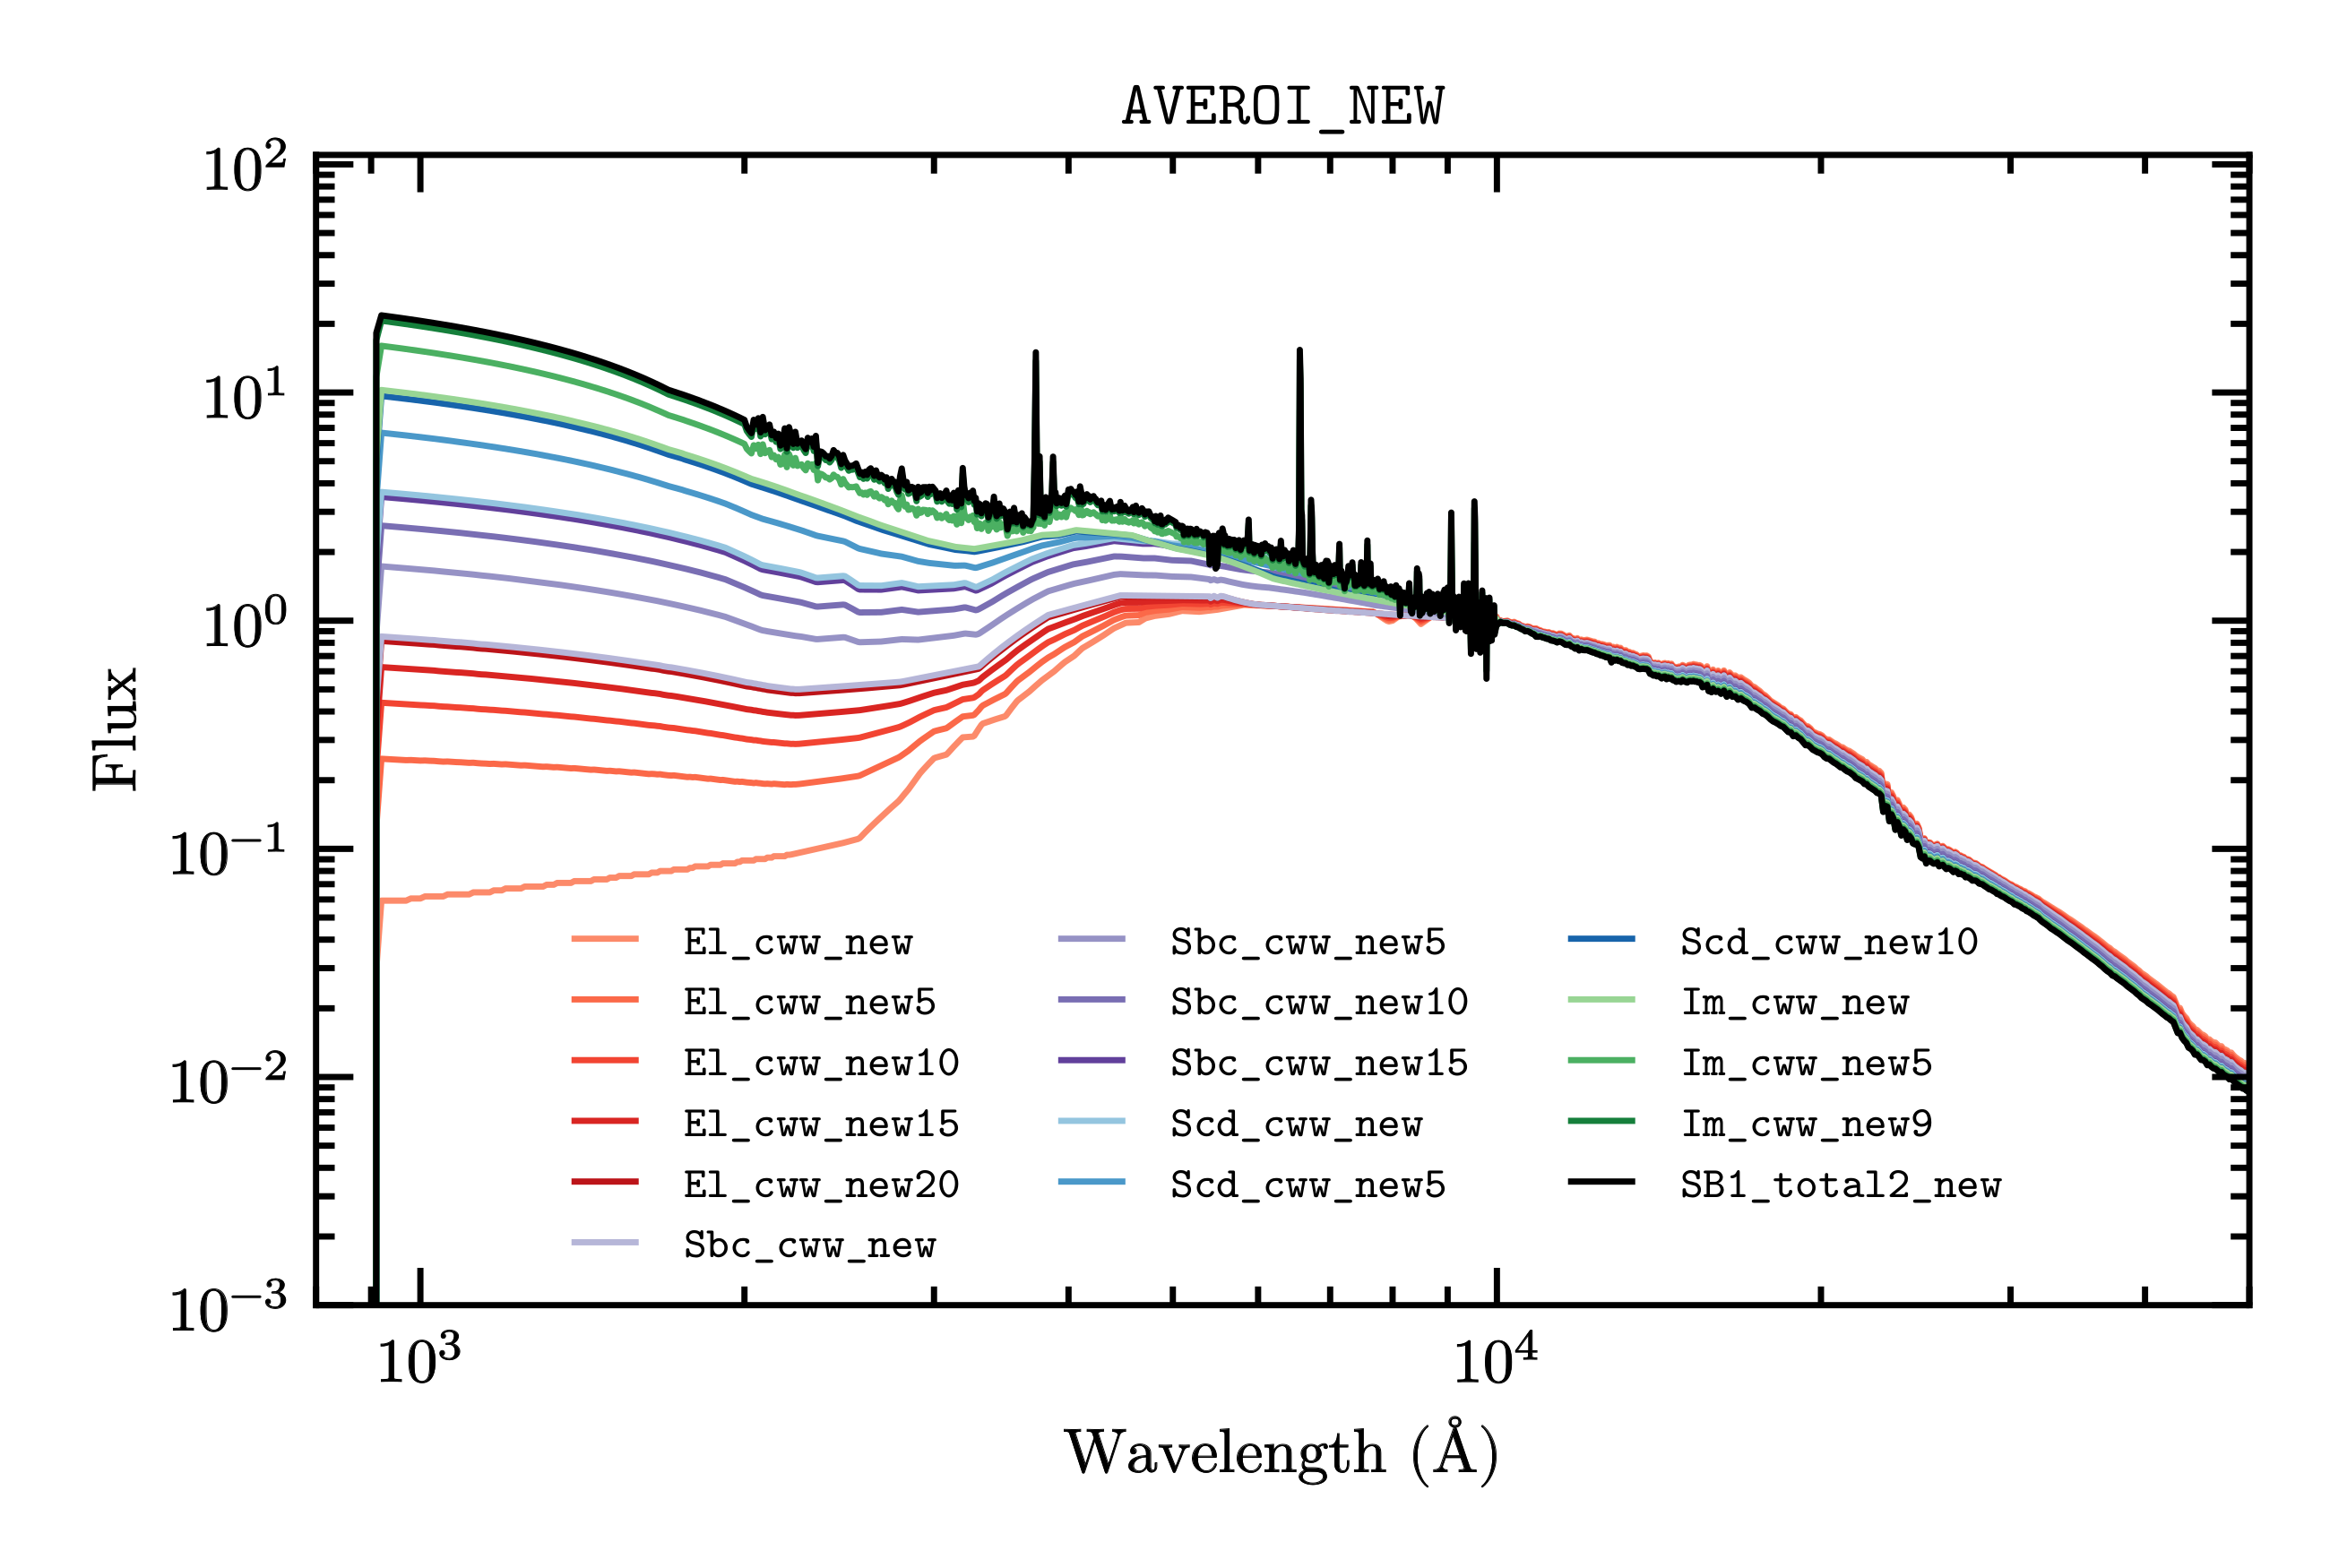
\includegraphics[clip, width=0.95\textwidth]{lephare_template_plots_averoin.png}}

\subfloat[\label{fig:templates_cosmos}]{
	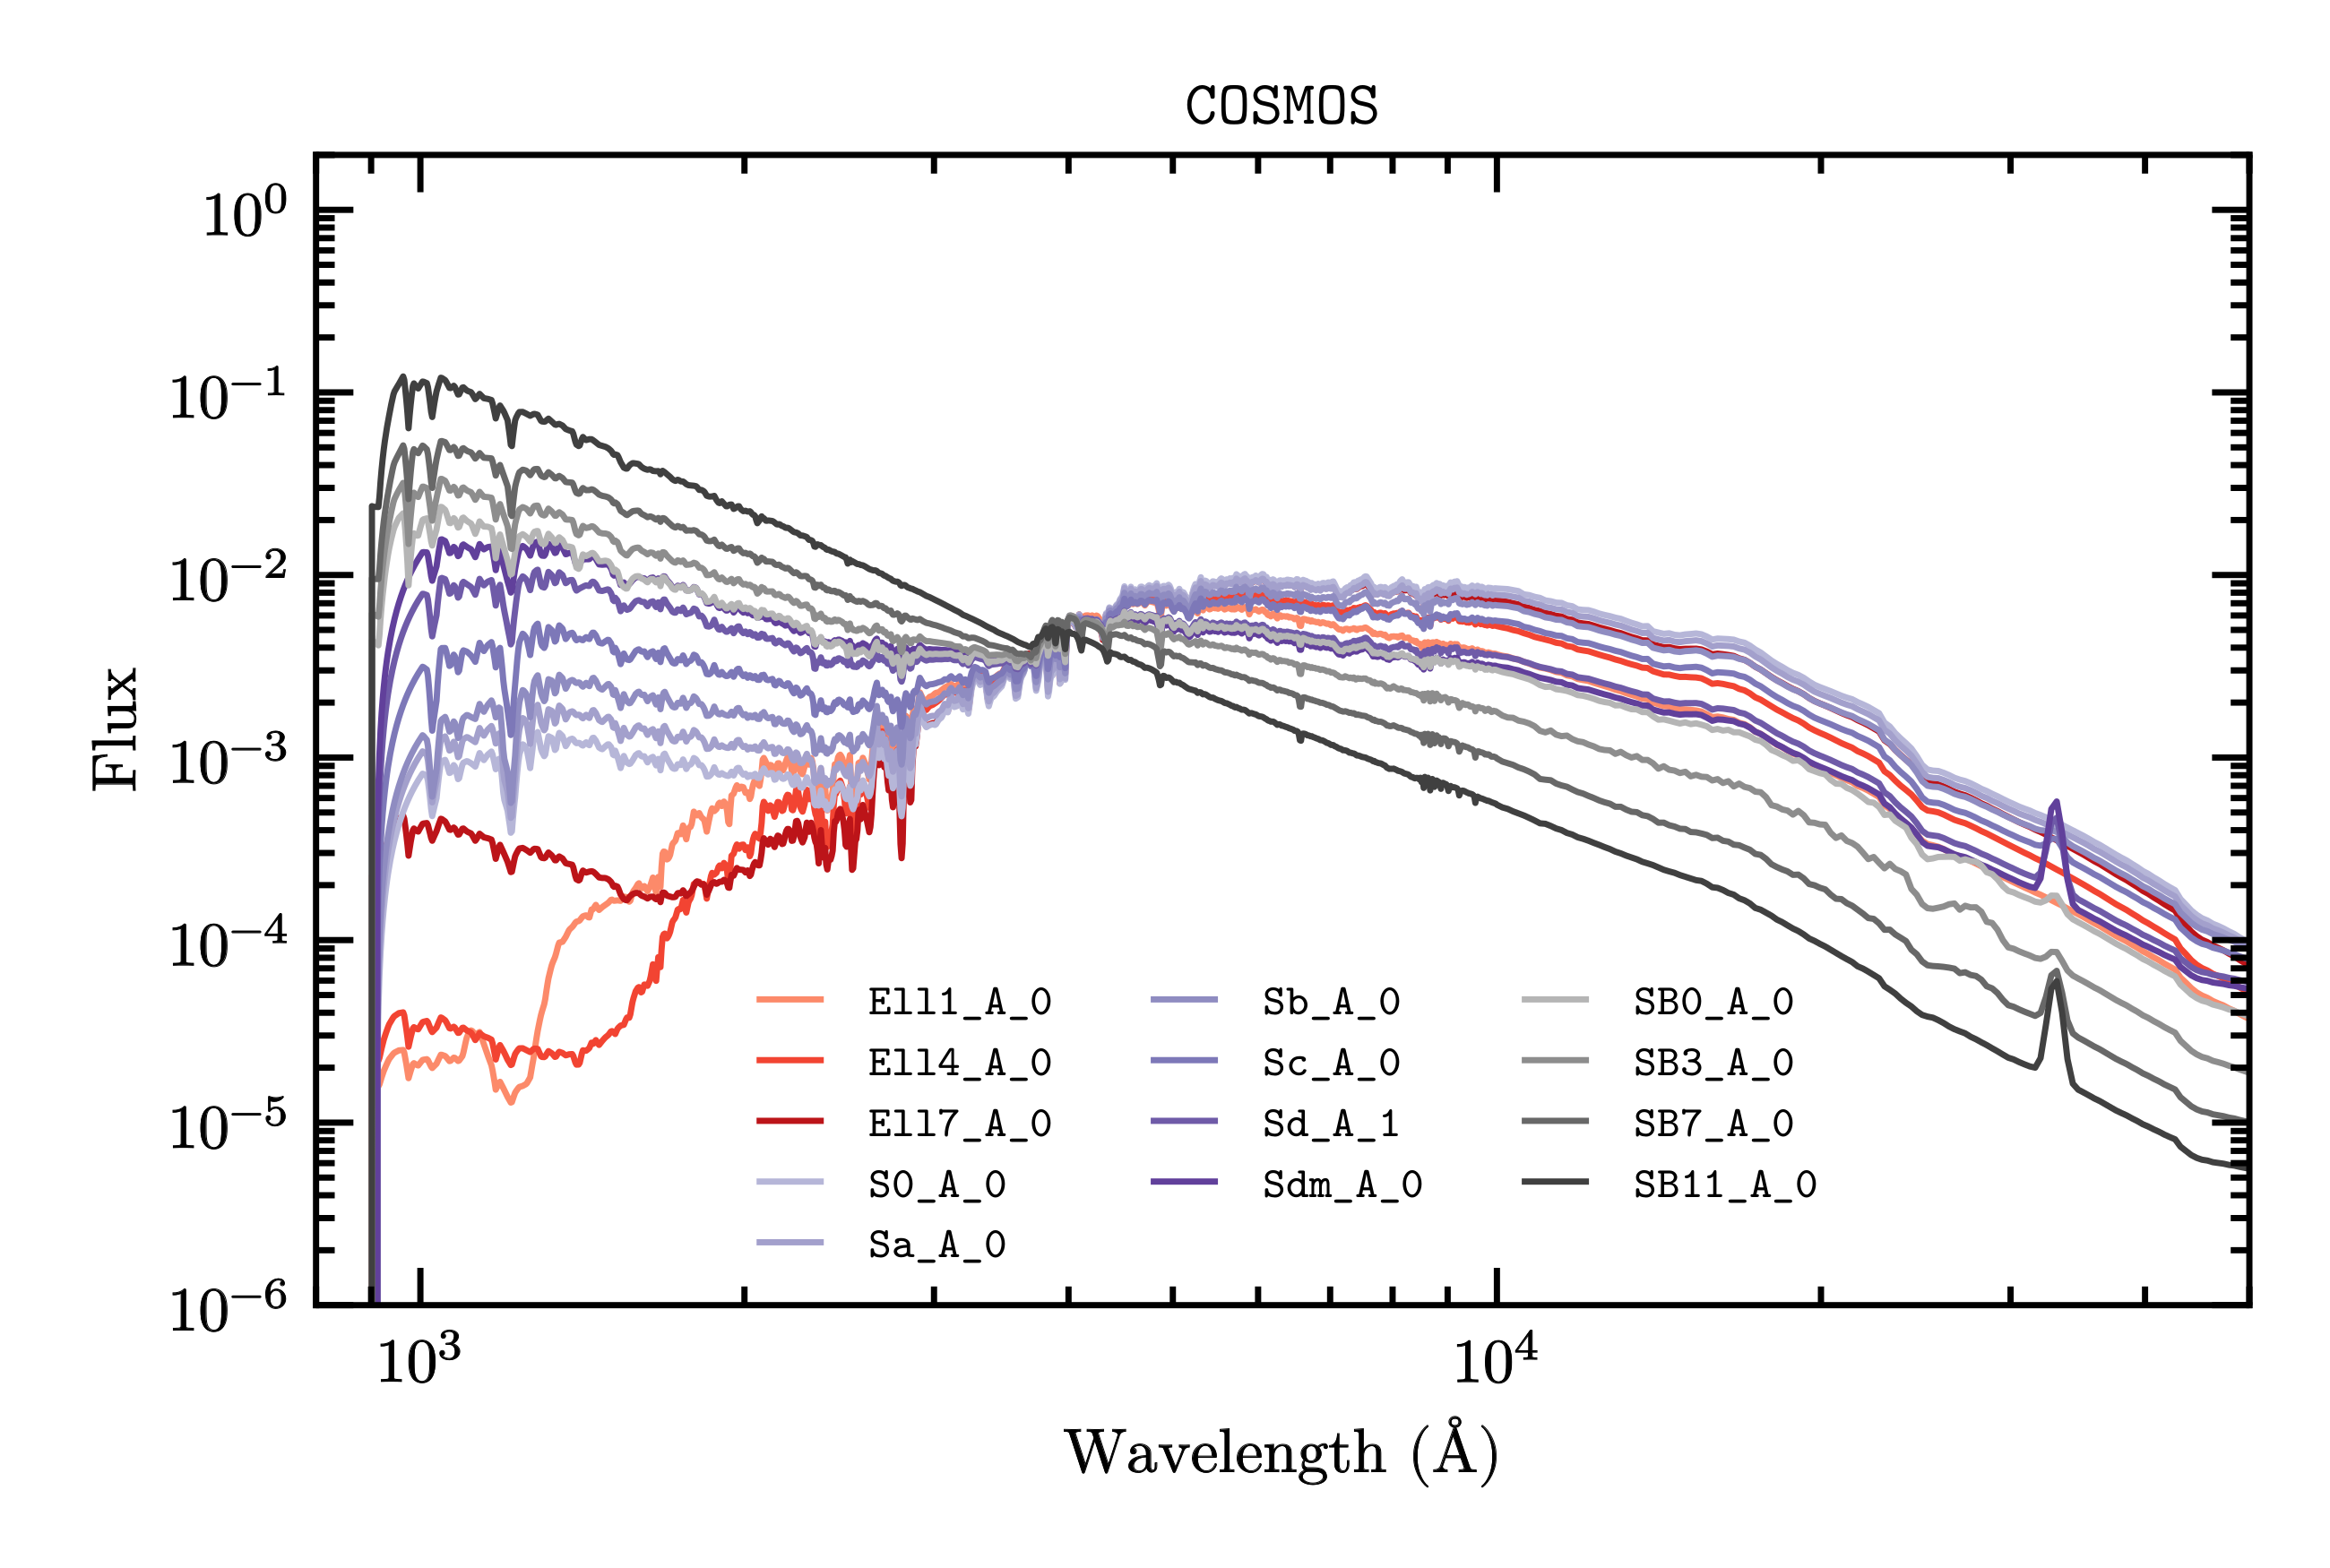
\includegraphics[clip, width=0.95\textwidth]{lephare_template_plots_cosmos.png}}
\caption[Galaxy template SEDs]{Spectra for the two sets of templates used to calculate photometric redshifts for the \DESVIDEO catalogue. The plots display a subset of templates covering a representative fraction of the full template set for \textbf{(a)} the \texttt{AVEROI\_NEW} templates and \textbf{(b)} the \texttt{COSMOS} templates. The names of these templates have been copied directly from the \texttt{LePHARE} installation. Broadly following the Hubble classification scheme for galaxy morphologies, spectra beginning in \texttt{El} or \texttt{Ell} correspond to elliptical galaxies, \texttt{Im} to irregular galaxies, \texttt{SB} to starburst galaxies, \texttt{S0\_A\_D} to a lenticular galaxy, and the other names starting in \texttt{S} to various forms of spirals.}
\label{fig:templates}
\end{figure*}

%among the plethora of photo-z studies

The CWW spectra that form the basis of the \texttt{AVEROI\_NEW} SEDs are a common choice of template among photo-z studies in the literature (e.g. \citealt{1999ApJ...513...34F,1999MNRAS.310..540A}), especially when augmented by starburst templates \citep{1997AJ....113....1S,2006ApJS..162...20B,2006A&A...457..841I}. For the CWW+starburst sets in particular, this choice enjoys strong observational support, as the combination of these templates has been shown to span the range of galaxy properties observed in the Hubble Deep Field over a wide redshift range of $0 < z < 6$ \citep{2000ApJ...536..571B,2002MNRAS.330..889F}. This completeness well into the high-redshift regime suggests that the \texttt{AVEROI\_NEW} templates make a highly appropriate choice for this thesis. \par


 

\subsubsection{\texttt{COSMOS} templates}\label{subsubsection:COSMOS}
The \texttt{COSMOS} template set consists of 31 theoretical SEDs assembled by \cite{2009ApJ...690.1236I} for their photo-z study of the COSMOS field. Nine of these templates were initially created by \cite{2007ApJ...663...81P}, who used the GRASIL code \citep{1998ApJ...509..103S} to generate templates that fitted the observed UV to mid-IR broadband colours of spectroscopically confirmed objects in the VVDS survey \citep{2005A&A...439..845L}. Three of these spectra represent elliptical types and six are spiral types (S0, Sa, Sb, Sc, Sd, Sdm). \cite{2009ApJ...690.1236I} linearly interpolated these nine SEDs to produce 19 templates. Because this collection does not adequately sample the blue end of galaxy colour space, \cite{2009ApJ...690.1236I} generated 12 additional templates using \cite{2003MNRAS.344.1000B} models with starburst ages from 0.03 to 3 Gyr, and extended these beyond 3 $\mu$m using the Sdm \cite{2007ApJ...663...81P} template. Together, all 31 SEDs form the \texttt{COSMOS} template set. Figure \ref{fig:templates_cosmos} shows a subset of these spectra.\par 


Because the \texttt{COSMOS} SEDs have been selected to fit the UV-mid-IR colours of an observed sample, \cite{2009ApJ...690.1236I} claim that they provide a better joining of the UV and mid-IR than  template sets based on the CWW spectra (such as the \texttt{AVEROI\_NEW} templates), which have been extrapolated from the optical theoretically. For this reason, it was deemed of interest to this thesis to test the \texttt{COSMOS} templates as well. Moreover, the \texttt{COSMOS} SEDs have also produced noteworthy observational success. As described above, they were used by \cite{2009ApJ...690.1236I} in the production of their COSMOS 30-band photometric redshift catalogue. Section \ref{subsubsection:multiwavelength_redshifts} previously mentioned
that this catalogue is extremely accurate, with a dispersion of only $\sigma_{\Delta z/ (1+z_{\mathrm{spec}})} =0.007$ (for the brightest $i^{+}_{\mathrm{AB}}<22.5$). \cite{2009ApJ...690.1236I} also demonstrated a 3--5 times improvement in accuracy compared to the previous 16-band COSMOS catalogue \citep{2007ApJS..172..117M} and CFHTLS-Deep results \citep{2006A&A...457..841I}, which were both based on modified versions of the CWW templates. Even though the exceptional accuracy is almost certainly for a large part thanks to the remarkable 30-band coverage, it also corroborates the quality of the \texttt{COSMOS} templates, and suggests that these may be an suitable choice for this thesis. The indicated improvement over CWW+starburst template sets is also interesting, and warrants a comparative investigation with the \texttt{AVEROI\_NEW} performance using the \DESVIDEO dataset.  



\subsection{Stellar and QSO templates}\label{subsection:star_qso_templates}
In addition to galaxy SEDs, \texttt{LePHARE} also determines the best-fit solutions for stellar and quasar (QSO) templates. This feature can be useful, because a comparison of the best-fit $\chi^2$ for each SED type can identify whether the observed colours of a given source are most consistent with a galaxy, a star, or a quasar.
Because stellar sources will have nonsensical photo-zs, they can contaminate photometric redshift catalogues, so it is important to have an effective method for differentiating between stars and galaxies. This task will be addressed in Section \ref{subsection:star_galaxy}, which will describe the process of finding a suitable star-galaxy separation method based on the SED fitting with \texttt{LePHARE}. Rejecting stars and low-redshift QSOs is also be important to the high-redshift galaxy search, so this thesis makes extensive use of the template fitting feature in Chapter \ref{chapter:high_redshift_candidates} as well. \par


To make sure that \texttt{LePHARE} can fit stars accurately, it is important to include a good selection of stellar SEDs. For this reason, it was decided to use the broadest set of stars contained in the default \texttt{LePHARE} installation. This collection consists of a total of 254 templates, composed of 131 empirical star SEDs from \cite{1998PASP..110..863P}, 4 observed white dwarf spectra from \cite{1995AJ....110.1316B}, 18 theoretical models of late-type stars, and a collection of 99 low mass stars and brown dwarfs from \cite{2000ApJ...542..464C}. Having a large selection of SEDs to cover the colours of low mass stars as comprehensively as possible is especially important for this thesis, since low mass stars and brown dwarfs are known to be major contaminants of $z\gtrsim5$ candidates \citep{2009MNRAS.395.2196M,2013AJ....145....4W,2015MNRAS.452.1817B,2016PASA...33...37F}. \par


%LABELLED X IN THE DEFAULT INSTALLATION
The QSO templates used in this thesis are based on models by \cite{2009ApJ...690.1250S}, and are taken from a collection labelled \texttt{QSO\_MARA} in the default \texttt{LePHARE} installation. These models contain  AGN-to-total luminosity ratios of $0.1<L_{\mathrm{AGN}}/L_{\mathrm{tot}}<0.9$, which cover a range of relative contributions to the combined spectrum from AGN or host galaxy emission. \par


\subsection{Extinction}\label{subsection:extinction}
All the templates presented so far are intrinsic SEDs, which do not include the effects of reddening by dust. Instead, \texttt{LePHARE} applies the necessary corrections for dust extinction itself, during the stage where it computes the predicted template magnitudes for Equation \ref{eqn:chi_squared} (see Section \ref{subsubsection:chi_minimisation}). The basic mechanism of dust extinction and its implementation in the code will be briefly described below. \par



Dust grains cause reddening of galaxy spectra by absorbing high energy UV and optical starlight and re-radiating it thermally at IR and submillimeter wavelengths. At a given wavelength $\lambda$ this process causes a shift $A_{\lambda}$ in the observed magnitude compared to the intrinsic (i.e. non-reddened) magnitude:

\begin{equation}
m_{\mathrm{obs}}(\lambda) = m_{\mathrm{int}}(\lambda) + A_{\lambda},\label{eqn:attenuation}
\end{equation}

\noindent where $m_{\mathrm{obs}}$ and $m_{\mathrm{int}}$ are the observed and intrinsic magnitudes respectively, and the shift $A_{\lambda}$ is what is referred to as the extinction (or attenuation). The wavelength dependence of $A_{\lambda}$ is customarily captured by the extinction curve $k(\lambda)$, which is defined as: 


\begin{equation}
k(\lambda) = \frac{A_{\lambda}}{E(B-V)}.\label{eqn:extinction_curve}
\end{equation}

\noindent Here, $E(B-V)$ is a reddening parameter which is equal to the discrepancy between observed and intrinsic $B-V$ colour:
 

\begin{equation}
E(B-V) = (B-V)_{\mathrm{obs}}-(B-V)_{\mathrm{int}}.\label{eqn:eb_v}
\end{equation}

The exact shape of the extinction curve $k(\lambda)$ depends on the content of the interstellar medium, which differs among galaxies.  A functional form has been found for a small number of local objects, notably the Milky Way \citep{1979MNRAS.187P..73S,1976MNRAS.174P..29A}, Large Magellanic Cloud (LMC; \citealt{1986AJ.....92.1068F}), Small Magellanic Cloud (SMC; \citealt{1984A&A...132..389P}; see Figure \ref{fig:extinction}), and starburst galaxies (\citealt{2000ApJ...533..682C}; see Figure \ref{fig:extinction}).  \texttt{LePHARE} allows the user to specify an extinction law and includes the extinction curves from the above studies by default. When applying extinction, the user must also provide a range of values for $E(B-V)$. With these user-specified choices for $k(\lambda)$ and $E(B-V)$, $A_{\lambda}$ can be inferred from Equation \ref{eqn:extinction_curve} and applied to the template SEDs via Equation \ref{eqn:attenuation}, to compute predicted galaxy magnitudes for varying amounts of dust attenuation. \par


For the purpose of this thesis, it was decided to follow the recommended dust extinction procedure for each template set as specified in the \texttt{LePHARE} documentation\footnote{More specifically, in the \texttt{README} files of the default installation.}. Following these instructions, the \texttt{AVEROI\_NEW} templates of star-forming galaxies are attenuated via the  SMC extinction curve. For the \texttt{COSMOS} templates, the SMC law is applied to the redder star-forming galaxies, and the Calzetti law is used for the bluest starburst galaxies. The specific details of the application of dust extinction will be addressed in Section \ref{section:setups}. \par



\begin{figure*}[h]
\centering
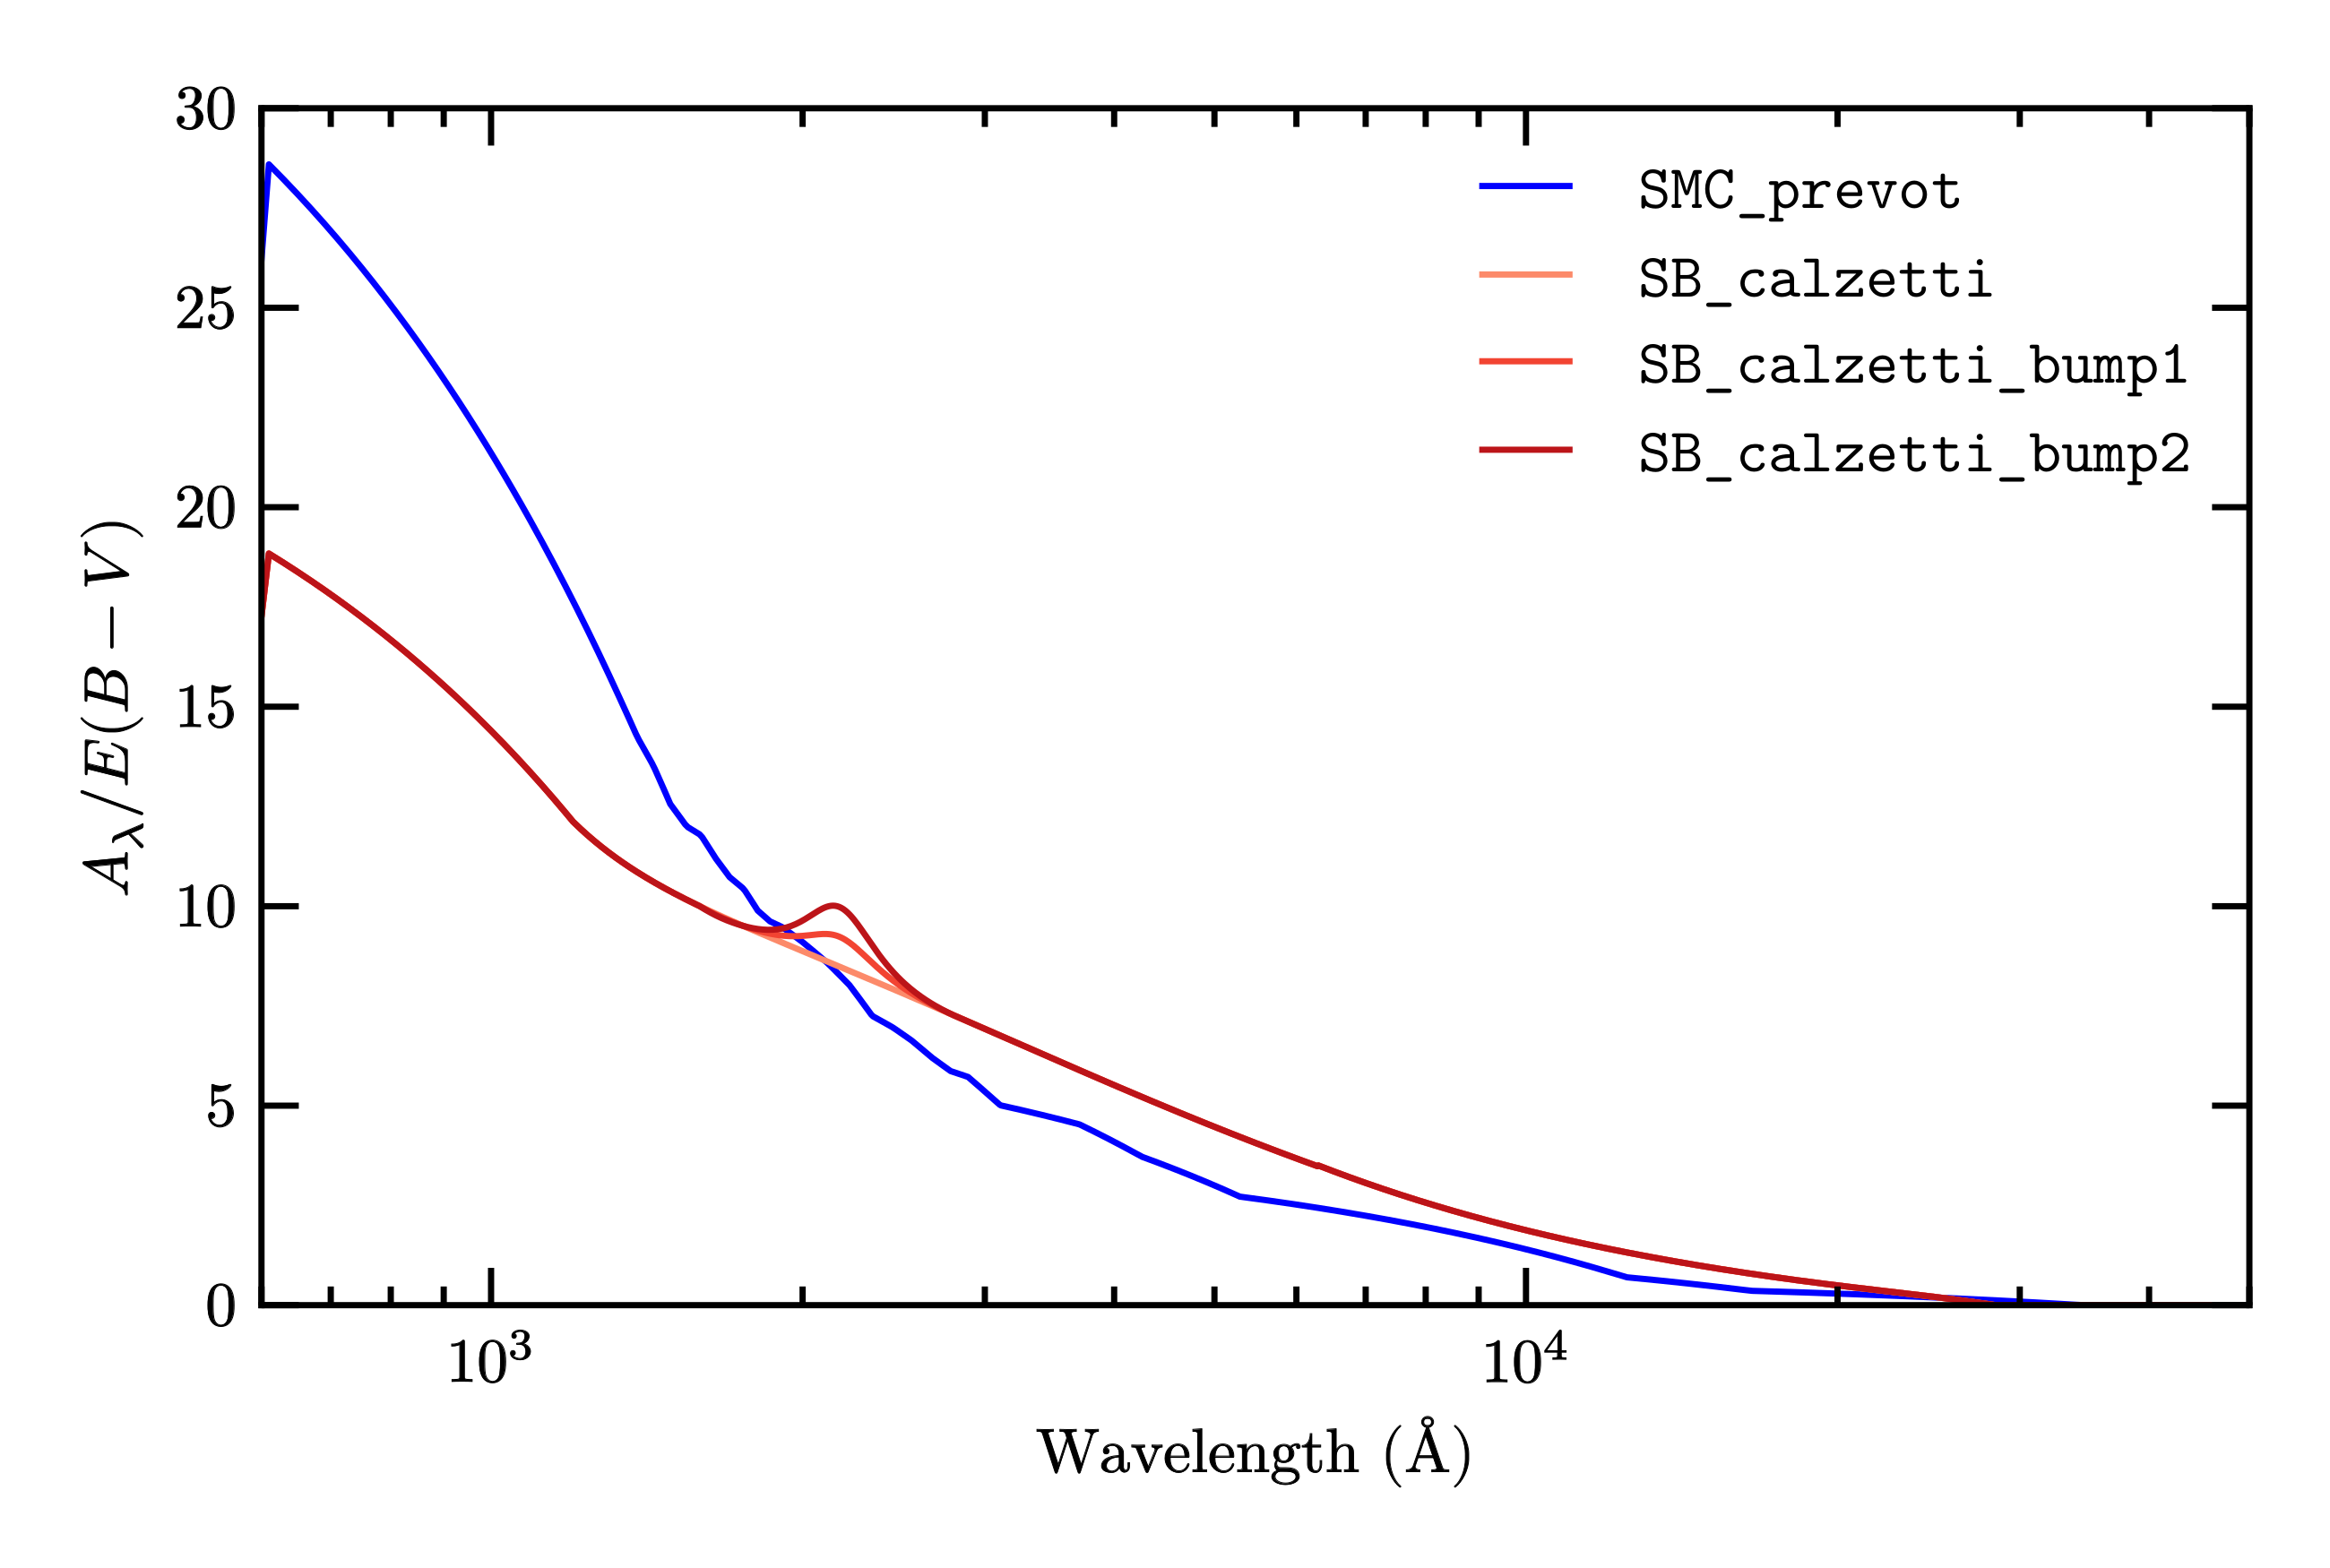
\includegraphics[width=0.95\textwidth]{lephare_extinction_plot.png}
\caption[Dust extinction curves]{Dust extinction curves $k(\lambda) = A_{\lambda} / E(B-V)$ for the SMC \citep{1984A&A...132..389P} and \cite{2000ApJ...533..682C} attenuation laws as included in the default \texttt{LePHARE} installation. There are three available options for the \cite{2000ApJ...533..682C} law, which have differing strengths of the \SI{2175}{\angstrom} bump (see e.g. \citealt{1965ApJ...142.1683S,1994ApJ...422..176M,2011ApJ...733...91X} for more information on this feature).}
\label{fig:extinction}
\end{figure*}


\subsection{Emission lines}\label{subsection:emission_lines}
To ensure that predicted template magnitudes are maximally accurate, it is important to consider the effect of emission lines.  \cite{2009ApJ...690.1236I} argue that strong emission lines can cause notable changes in colour even in broadband filters (up to $\sim0.15$ mag), and that for accurate photometric redshifts, emission lines must therefore be taken into account. \par

There is an option within \texttt{LePHARE} to add Ly$\alpha$, H$\alpha$, H$\beta$, [$\mathrm{O_{II}}$], and [$\mathrm{O_{III}}$] emission lines to the galaxy templates. This feature has been implemented via a process described in \cite{2009ApJ...690.1236I}, which infers the emission line strengths from template UV fluxes. Via a relation from \cite{1998ARA&A..36..189K}, the UV luminosity is firstly used to estimate the global star formation rate (SFR):

%I GOT UP TO HERE. UNITS!!!!!!

\begin{equation}
\mathrm{SFR} (M_{\odot}\mathrm{yr^{-1}} ) = 1.4 \times 10^{-28} L_{\nu,\mathrm{UV}} (\mathrm{erg \ s^{-1} \ Hz^{-1}} ),\label{eqn:kennicut}
\end{equation} 

\noindent which can be related to the [$\mathrm{O_{II}}$] emission line luminosity via:

\begin{equation}
\mathrm{SFR} (M_{\odot}\mathrm{yr^{-1}}) = (1.4 \pm 0.4) \times 10^{-41} L_{[\mathrm{O_{II}}]} (\mathrm{erg \ s^{-1}}).\label{eqn:sfr_oii}
\end{equation}

Putting Equation \ref{eqn:kennicut} and \ref{eqn:sfr_oii} together, and converting luminosity to flux or magnitude, \cite{2009ApJ...690.1236I} obtain:


\begin{equation}
\log{ \left\{ F_{[\mathrm{O_{II}}]}(10^{-17}\mathrm{erg \ s^{-1} cm^2}) \right\} } = -0.1 \times M_{\mathrm{UV}} +10.65 -\frac{DM(z)}{2.5},
\end{equation}

\noindent where $F_{[\mathrm{O_{II}}]}$ is the [$\mathrm{O_{II}}$] line flux, $DM(z)$ is the distance modulus, and $M_{UV}$ is the UV absolute magnitude measured at \SI{2300}{\angstrom} from the (dust-corrected) template SEDs. Because \texttt{LePHARE} can directly measure the latter two quantities, it is able to measure the value of $F_{[\mathrm{O_{II}}]}$ for each (redshifted) template. It then estimates the other emission lines from their intrinsic, unextincted flux ratios with [$\mathrm{O_{II}}$]: $[\mathrm{O_{III}/O_{II}}]=0.36$, $[\mathrm{H}\beta/\mathrm{O_{II}}] = 0.61$, $[\mathrm{H}_{\alpha}/\mathrm{O_{II}}] =1.77$, and $[\mathrm{H}_{\alpha}/\mathrm{O_{II}}] = 2$ \citep{1985ApJS...57....1M,2006ApJ...642..775M,2005MNRAS.362.1143M,1998ARA&A..36..189K}. To obtain the final line strengths, these values are corrected with the appropriate attenuation. At the end, the code adds all the emission lines to the desired predicted magnitudes for the template fitting in \ref{eqn:chi_squared}. It only applies emission lines to templates with a dust free colour bluer than $(NUV-r)_{\mathrm{ABS}} \leq 4$. \par


\section{Photometric redshift configurations}\label{section:setups}
Now the proposed photometric redshift code and template SEDs have been presented, the next step is to introduce the input details for the code. The previous few sections have mentioned several options and parameters in \texttt{LePHARE} that must be specified by the user. The values of these, and various other required inputs, can be provided in configuration files. Throughout this thesis, a particular configuration is referred to as a `setup'. For the \DESVIDEO dataset, a number of setups with different parameters have been tested and compared in terms of their photometric redshift performance, which is assessed by comparing the photo-zs for spectroscopically confirmed galaxies to their measured spectroscopic redshifts. The current section will introduce all these different test configurations.  Afterwards, Section \ref{section:photoz_computation} will then describe the process of computing the photo-zs and various performance assessment measures, which will be analysed in detail in Section \ref{section:photoz_discussion}. \par

 
The photo-z tests have been conducted on the spectroscopic \DESVIDEO subsample only (see Section \ref{subsection:spectra}). The objective is to find the optimal configuration (judged primarily by high-redshift performance) for both the \texttt{AVEROI\_NEW} and \texttt{COSMOS} SEDs, previously introduced in Section \ref{subsection:galaxy_templates}.  The end of this chapter will describe how these setups are used to compute photometric redshifts for the full \DESVIDEO catalogue. There are several reasons for studying two sets of templates in detail. Firstly, computing photo-zs with several template sets makes the \DESVIDEO catalogue more useful as a general resource, as future users will be able to choose which template set is best suited to their particular research. Secondly, the discussion in Section \ref{subsubsection:COSMOS} offered some indications that the \texttt{COSMOS} templates might provide more accurate photo-zs than the \texttt{AVEROI\_NEW} SEDs, which suggests that it is interesting to use the \DESVIDEO data to compare their performance in detail. Thirdly, as one of the aims of this thesis is to perform a precise investigation of how the setup choice impacts photo-zs, the use of different templates provides a better template-independent means of assessing the effect of each configuration parameter.\par


\subsection{The \texttt{default} configurations}\label{subsection:default}
A first attempt at a suitable setup for either template set was constructed by the author, based on a configuration created by \cite{2013MNRAS.428.1281J} for a very similar dataset, and on findings by previous studies. These two setups are subsequently referred to as `\texttt{default}', and the corresponding configuration file for the \texttt{AVEROI\_NEW} templates is shown in full in Appendix \ref{appendix:config_lephare}. \par


\subsubsection{Templates}
The first \texttt{default} input file uses the \texttt{AVEROI\_NEW} templates. To recap, Section \ref{subsubsection:AVEROI_NEW} mentioned that these SEDs were chosen based on the consideration that similar CWW+starburst template combinations have been successful in  many photo-z studies, and that they have been shown to represent galaxies all the way out to $z\sim6$. Following recommendations in the \texttt{LePHARE} documentation, the SMC extinction curve (see Figure \ref{fig:extinction}) is applied to all Scd, irregular (Im in Figure \ref{fig:templates_averoin}) and starburst (SB in Figure \ref{fig:templates_averoin}) spectral types, with $E(B-V)$ values of 0.0, 0.05, 0.1, 0.15, 0.2, 0.3, 0.4, 0.5, 0.7, 1.0. This range is larger than the recommended values listed in the \texttt{README} file of the \texttt{LePHARE} installation, which instead suggests a maximum permitted value of $E(B-V)=0.3$. The higher \texttt{default} maximum was chosen in order to capture very red dusty galaxies, which can contaminate samples of high-redshift candidates (however, the original recommendation of $E(B-V)\leq0.3$ will also be tested via an alternative configuration presented shortly in Section \ref{subsection:alternative_setups}). Finally, the \texttt{AVEROI\_NEW default} configuration adds emission lines to the templates, on the basis that \cite{2009ApJ...690.1236I} claimed that this improves the photometric redshifts (see Section \ref{subsection:emission_lines}).\par

The second \texttt{default} setup uses the \texttt{COSMOS} SEDs. Earlier on, Section \ref{subsubsection:COSMOS} suggested that these templates may be a suitable choice based on previous observational success. In the \texttt{COSMOS default} configuration, dust extinction is applied with values of $E(B-V) = 0.0, 0.1, 0.2, 0.3, 0.4, 0.5$. The Calzetti extinction law (see Figure \ref{fig:extinction}) is applied to the SB3 galaxy type and all bluer types (the reader is referred to Figure \ref{fig:templates_cosmos} for a clarification of the \texttt{COSMOS} spectral types), and the SMC law (see Figure \ref{fig:extinction}) is applied to all types redder than SB3 (including SB3). No extinction is applied to galaxies redder than Sb. The Calzetti law is applied three times, once for each of the three strengths of the \SI{2175}{\angstrom} bump in Figure \ref{fig:extinction}. All the above decisions directly follow the recommendations in the \texttt{LePHARE} installation, which are also covered in \cite{2009ApJ...690.1236I}. For the same reasons listed for the \texttt{AVEROI\_NEW} templates, emission lines are enabled for the \texttt{COSMOS} \texttt{default} configuration.\par 



\subsubsection{Photometric redshift code options for the \texttt{default} configurations}\label{subsubsection:photoz_options_default}
Sections \ref{subsection:prior} and \ref{subsection:adaptive_offsets} introduced two options in \texttt{LePHARE} designed to aid in the redshift estimations. The \texttt{default} setups each use both these features, discussed below and implemented as described.\par


\paragraph{$N(z)$ prior} The \texttt{default} configurations both enable the option to apply a luminosity prior $N(z)$, described in Section \ref{subsection:prior}. The discussion there described how the use of a prior is likely to be helpful for this thesis, as it has been shown to reduce outliers. As mentioned, the $N(z)$ prior in \texttt{LePHARE} refers to the $B-I$ colour of objects in the VVDS. While the DES observations naturally do not include $B$-band data, \cite{2014MNRAS.445.1482S} have demonstrated that DES $g-i$ colour is a reasonable substitute, so the \texttt{default} configurations use these two filters as input for the prior. \par



\paragraph{Adaptive offsets}Section \ref{subsection:adaptive_offsets} presented several reasons why the inclusion of adaptive offsets, which calibrate zero-point offsets via spectroscopic redshifts, might be beneficial for the \DESVIDEO catalogue. In particular, the ability to incorporate aperture corrections, and the capacity to compensate for uncertainties in the photometric zero-point calibration are considered especially important to this thesis. With these arguments in mind, it was decided to activate this option in the \texttt{default} configurations. \par

Inconveniently, a quick first attempt at calculating suitable adaptive offsets for each \DESVIDEO tile revealed that the offsets determined by \texttt{LePHARE} vary considerably from tile to tile. This is not unexpected --- differences in imaging quality and cosmic variance can cause such an effect in several ways. For starters, the seeing fluctuates across tiles, which leads to different compensation for aperture corrections. Secondly, due to the varying depth and cosmic variance, the galaxy populations observed in each tile are different as well. Because of the effect that template incompleteness can have on the adaptive offset values, differences in spectral types can lead to disparity in the offsets. \par

The reasoning above implies that the adaptive offsets would be most accurate when computed on a DES tile-to-tile basis. Unfortunately, some DES tiles contain an insufficient number of spectroscopic redshifts to make the calculated values statistically sound (e.g. there exist 19 DES tiles with <100 spectra). However, each of the eight VIDEO tiles does include a sizeable number (>1000) of spectra. It was therefore decided to compute the adaptive offsets individually for each VIDEO tile. This ensures that the offsets are based on VIDEO imaging with constant limiting magnitudes. There are still depth differences among each of the DES co-adds covering a given VIDEO tile, but this variation is generally smaller than the DES variation over the full footprint (see Figures \ref{fig:depth_es1}, \ref{fig:depth_xmm}, and \ref{fig:depth_cdfs}). Therefore, the proposed strategy method provides a good balance, allowing the adaptive offsets to capture most of the depth variation, while also ensuring that they are based on a statistically sound number of spectra. \par

Because the uncertainties in the adaptive offsets computed by \texttt{LePHARE} are not better than \SI{0.01}{\mag} \citep{2009ApJ...690.1236I}, a value of 0.01 is added in quadrature to the apparent magnitude errors in the input photometry\footnote{This is taken care of by specifying a value of \SI{0.01}{\mag} for the \texttt{ERR\_SCALE} parameter, which leads \texttt{LePHARE} to increase the errors automatically.}. 

\subsubsection{Input photometry for the \texttt{default} configurations}\label{subsubsection:input_phot_default}
Naturally, in order to be able to compute photometric redshifts, \texttt{LePHARE} requires the user to supply input photometry. For the \texttt{default} setups, these input files consist of fluxes in all the \DESVIDEO $grizZYJHK_{s}$-bands (note that this excludes the DES $Y$-band, which is too shallow compared to the other bands to be useful for the photo-zs in this thesis), measured in a fixed \SI{1.95}{\arcsec} diameter aperture. The choice for fixed-size aperture fluxes over auto photometry was mirrored on similar studies in the literature (e.g. \citealt{2009ApJ...701.1839M,2013MNRAS.428.1281J,2012MNRAS.426.2772B,2014MNRAS.440.2810B}). The relatively small \SI{1.95}{\arcsec} size was chosen because high-redshift candidates are expected to be faint, and measuring fluxes over too large an aperture compromises the signal-to-noise for faint sources \citep{2019NatAs...3..212S}. The aperture diameter is therefore designed to be not much larger than the expected spatial extent of $z\gtrsim5$ galaxies. In previous ground-based surveys with similar seeing, galaxy sizes around $z\sim6$ have generally been dominated by the seeing \citep{2013AJ....145....4W,2014MNRAS.440.2810B,2015MNRAS.452.1817B}. Given that the DES and VIDEO FWHM is around $\sim\SI{1}{\arcsec}$, \SI{1.95}{\arcsec} apertures are expected to enclose the majority of galaxy flux, while also being small enough to minimise photometric noise. A comparable \SI{2}{\arcsec} diameter has also been used by previous studies with similar datasets \citep{2013MNRAS.428.1281J,2012MNRAS.426.2772B}, and has been shown to deliver good results at low redshifts as well \citep{2009ApJ...701.1839M,2013MNRAS.428.1281J}. \par 


\subsection{Alternative configurations}\label{subsection:alternative_setups}
To investigate the effect of different input parameters on the photo-zs, the performance of the \texttt{default} setup for both template sets is compared to other possible configurations. Each of these rival setups is identical to the \texttt{default} version with the exception of one factor. This section presents all the alternative setups for this investigation, alongside a clarification of which parameters have been changed. \par

{\vspace{1em plus 0.2em minus 0.1em}}
\textit{The configurations for the following four setups are template dependent, and are defined individually for each template set:} \par

\subparagraph{\texttt{AVEROI\_NEW less\_ext}} This setup uses the original extinction recommendation found in the \texttt{README} file for the \texttt{AVEROI\_NEW} templates in the \texttt{LePHARE} installation. These values equal $E(B-V)=0.0,0.05,0.10,0.15,0.20,0.25,0.30$. The aim of this setup is to investigate whether this lower extinction range is sufficient to produce accurate photo-zs, by testing whether it performs as well as (or better than) the wider range of up to $E(B-V)=1.0$ used in the \texttt{default} setup. 

\subparagraph{\texttt{AVEROI\_NEW more\_ext}} As emphasised throughout this chapter, a priority for the \DESVIDEO photo-zs is optimal performance at $z\gtrsim5$. Very red dusty galaxies are a known contaminant at these redshifts \citep{2016PASA...33...37F}, because their extremely red colours replicate those of true high-redshift sources in some filters. The \texttt{more\_ext} setup tests whether maximally reducing contamination at high redshifts requires even higher extinction than the \texttt{default} values, in order to capture adequately the colours of any extremely red low-redshift interlopers. The permitted extinction range in the \texttt{more\_ext} setup equals $E(B-V) = 0.0, 0.05, 0.1, 0.15, 0.2, 0.3, 0.4, 0.5, 0.7, 1.0, 1.3, 1.6, 2.0$. 

\subparagraph{\texttt{COSMOS} \texttt{ext}, \texttt{more\_ext}} The \texttt{default} setup for the \texttt{COSMOS} templates uses extinction values of up to $E(B-V)=0.5$. For the same reasons as for the \texttt{AVEROI\_NEW more\_ext} setup above, the \texttt{COSMOS} \texttt{ext} and \texttt{more\_ext} configurations test whether a larger amount of reddening is required for optimal (high-redshift) results. The permitted extinction values are $E(B-V)=0.0,\allowbreak 0.1,\allowbreak 0.2,\allowbreak 0.3,\allowbreak 0.4,\allowbreak 0.5,\allowbreak 0.7,\allowbreak 1.0$ for the \texttt{ext} setup, and $E(B-V)=0.0,\allowbreak 0.1,\allowbreak 0.2,\allowbreak 0.3,\allowbreak 0.4,\allowbreak 0.5,\allowbreak 0.7,\allowbreak 1.0,\allowbreak 1.3,\allowbreak 1.6,\allowbreak 2.0$ for the \texttt{more\_ext} configuration. \par

{\vspace{1.2em plus 0.2em minus 0.1em}}\textit{The remainder of the alternative setups are the same for both the \textup{\texttt{AVEROI\_NEW}} and \textup{\texttt{COSMOS}} template sets (i.e. each configuration contains the same change to the respective \textup{\texttt{default}} setups).} \par


\subparagraph{\texttt{no\_emlines}} To evaluate whether the photometric redshift accuracy improves by adding emission lines to the templates (as claimed by \citealt{2009ApJ...690.1236I}), emission lines are turned off in the \texttt{no\_emlines} setups.

\subparagraph{\texttt{no\_adapt}} The use of adaptive offsets is disabled in the  \texttt{no\_adapt} setups, in order to assess how the offsets affect the photo-z results. 

\subparagraph{\texttt{no\_prior}} Due to fact that known distributions of galaxies are heavily skewed towards low redshifts, including an $N(z)$ prior will inherently bias photo-z estimates against high-redshift solutions \citep{2000ApJ...536..571B}. This could potentially remove some genuine high-redshift galaxies from any resulting $z\gtrsim5$ sample. It is therefore interesting to investigate whether it is possible to avoid using a prior, while still maintaining a manageable level of high-redshift contamination by low-redshift interlopers. Interestingly, several results in the literature indicate that the inclusion of near-infrared photometry may help to break the colour-redshift degeneracies that can lead to those contaminating catastrophic outliers \citep{2000ApJ...536..571B,2006A&A...457..841I}. To investigate whether the \DESVIDEO catalogue does in fact contain enough photometric data to permit not using a prior, the \texttt{no\_prior} configurations test the photo-z performance without the use of an $N(z)$ prior. 
 

\subparagraph{\texttt{auto}} As mentioned previously in Section \ref{subsection:default}, it is common in the literature to use aperture magnitudes as input photometry, and the \texttt{default} configurations follow this custom. To test the validity of this assumption, the \texttt{auto} setups use an input catalogue based on auto fluxes instead. 



\subparagraph{\texttt{des}, \texttt{des\_auto}} While the default setups use data from all nine $grizZYJHK_{s}$ \DESVIDEO bands, the \texttt{des} and \texttt{des\_auto} configurations only include flux measurements from the DES $griz$ filters, using aperture and auto photometry respectively. By assessing the photo-z performance without the VIDEO data, these setups can probe the extent to which near-IR coverage improves the photometric redshifts.



\section{Configuration testing}\label{section:photoz_computation}
\subsection{Photometric redshift computation method}\label{subsection:photoz_computation_method}
The next stage in the investigation aims to quantify which is the most suitable configuration for the \DESVIDEO catalogue. To this end, photometric redshifts have been computed for the subset of galaxies with spectroscopic redshifts, using all of the 18 configurations introduced in the previous section (9 for each template set). The redshifts have been obtained via a procedure with several stages, which ensure that the resulting photo-zs are as reliable as possible. This algorithm consists of the following steps: 

\begin{enumerate}
    \item Firstly, the list of sources with spectroscopic redshifts (see Section \ref{subsection:spectra}) is combined with the \DESVIDEO dataset. To do this, the spectra are matched within a \SI{1}{\arcsec} radius to the \DESVIDEO tables from step 7 of the assembly pipeline in Section \ref{subsection:catalog_production}, i.e. the photometric catalogues for each combination of overlapping DES and VIDEO tiles. At this stage, the objective of the spectroscopic redshifts is to calibrate adaptive offsets. Therefore, in order to make sure that the input data for these offsets is maximally reliable, the algorithm removes spectroscopic objects with a bad \texttt{FLAGS\_WEIGHT} value in any DES or VIDEO band. This criterion also applies to the DES $Y$-band, which is not used in any subsequent photo-z computations. The reason why it is nonetheless included here relates to the need for reliable input fluxes. As described in Section \ref{subsubsection:data_quality}, the \texttt{FLAGS\_WEIGHT} value in a given band is non-zero if the object overlaps a region with bad data or no data in that filter. In the case of the DES data, these bad regions include chip gaps. The images in all DES bands are severely more noisy in the vicinity of these gaps, but the DESDM catalogue uncertainties have not been suitably adjusted to account for this, which results in unreliable photometry around those regions. Because the weight maps in the five $grizY$-bands have slightly different widths for the chip gaps, using the \texttt{FLAGS\_WEIGHT} parameter in all bands ensures the exclusion of as many objects as possible in the noisy border regions. 
    
    %\footnote{}
    
    %I GOT UP TO HERE
    
    \item For each VIDEO tile, the algorithm then merges the spectroscopic catalogues from step 1 together for all the \DESVIDEO tiles that overlap that VIDEO tile. In the merging process, any duplicate spectra from overlapping DES tiles are removed, so that the combined catalogues include each spectrum only once per VIDEO tile. The duplicates are removed by rejecting any objects that do not exist within the non-duplicate version of the DESDM catalogues (assembled previously by the author as described in Section \ref{subsubsection:duplicates}). 
    
    %THIS IS BECAUSE OF THE ADAPTIVE OFFSETS
    \item To calculate photometric redshifts, \texttt{LePHARE} is run individually on each of the VIDEO tiles, using all of the 18 setups introduced in Section \ref{section:setups} (9 for each template set). The input contains photometry and spectroscopic redshifts from the catalogues in step 2, and the output consists of the standard \texttt{LePHARE} output, which includes photometric redshifts for all sources, as well as adaptive offsets (for the configurations where they were enabled).  Running \texttt{LePHARE} in the above way automatically achieves the goal previously laid out in Section \ref{subsubsection:photoz_options_default}, of calibrating the adaptive offsets for each VIDEO tile individually. 
    
    \item For each configuration, the \texttt{LePHARE} results from all eight VIDEO tiles are then merged together. To achieve this, the algorithm stacks the eight output files from step 3. The objective of these merged datasets is to enable a statistical analysis of the photo-z performance for each setup (which will be described later in Section \ref{subsection:accuracy_metrics}). Initially, the simple stacked catalogues contain duplicates from the overlapping regions between tiles. While these duplicate objects were needed in the earlier steps to make sure that the adaptive offsets are based on a maximal number of spectra, they introduce bias in the statistics. Duplicates are therefore removed; when a single DES object is covered by multiple VIDEO tiles, the algorithm retains the data from the highest ranking VIDEO tile. The author determined this ranking from Table \ref{table:error_agreement}, based on the depths and available bands. In order of descending priority, the order is: (es1-north, es1-south) for the ELAIS-S1, (xmm3, xmm2, xmm1) for the XMM-LSS and (cdfs1, cdfs2, cdfs3) for the CDF-S. The final product is a series of 18 photo-z catalogues (one for each configuration), where each spectrum is included only once. 
    
\end{enumerate}

After the above algorithm was applied to the \DESVIDEO dataset, the resulting 18 photo-z catalogues each contain a total of \num{35596} sources with spectrocopic and photometric redshifts. \par


\subsection{Accuracy metrics for assessing photo-z performance}\label{subsection:accuracy_metrics}
The redshift catalogues from the previous section can be used to assess the photo-z performance of each configuration. To do so, this thesis uses eight accuracy metrics, largely following \cite{2014MNRAS.445.1482S}.  In this framework, the individual bias (i.e. the photometric-to-spectroscopic discrepancy) for each object $i$ is defined as $\Delta z_{i} = z_{\mathrm{phot},i}-z_{\mathrm{spec},i}$, and $N$ represents the total number of objects used in the estimation of the statistics. Using these notations, eight statistical measures have been defined to capture various aspects of the photo-z distribution:



\begin{enumerate}[label=(\roman*)]
\item \textbf{Bias}. Two metrics capture the average bias. The first of these is the mean bias $\overbar{\Delta z}$, which is defined as follows:
\begin{equation}
\overbar{\Delta z} = \frac{1}{N} \sum^{N}_{i} \Delta z_{i}. \label{eqn:bias}
\end{equation}
  
Secondly, the median bias $\Delta z_{50}$ corresponds to the median of the $\Delta z$ distribution, defined as the (interpolated) middle value of an ordered list of $\Delta z_{i}$ values. In other words, the median is the value of $\Delta z$ that satisfies the following equation:

\begin{equation}
 P_{50} \equiv P(\Delta z \leq \Delta z_{50}) = \frac{1}{2}. \label{eqn:median}
\end{equation}
 
\item \textbf{Scatter}. The scatter is measured by two separate statistics, corresponding to the two bias metrics defined above. Firstly, there is the standard deviation $\sigma$ of the mean bias $\overbar{\Delta z}$, which is expressed as: 

 \begin{equation}
 \sigma = \sqrt{\frac{1}{N} \sum^{N}_{i} (\Delta z_{i} - \overbar{\Delta z})}.
 \end{equation}

The second statistic measures the 68 percentile width $\sigma_{68}$ of the $\Delta z$ distribution about the median bias $\Delta z_{50}$; in other words, $\Delta z_{50} \pm \sigma_{68}$ encloses 68\% of the $\Delta z$ distribution:

\begin{equation}
\sigma_{68} = \frac{1}{2} (\Delta z_{84} - \Delta z_{16}),
\end{equation}
 
\noindent where $\Delta z_{84}$ and $\Delta z_{16}$ are defined analogously to $\Delta z_{50}$ in Equation \ref{eqn:median}. \par


In the specific case where the values of $\Delta z_i$ are normally distributed, it is the case that $\sigma = \sigma_{68}$. However, in general the bias distribution is not Gaussian, and $\sigma_{68}$ captures the scatter in the core of the $\Delta z$ distribution  $\sigma$ is more sensitive to the tails.\par  

\item \textbf{Outliers}. The number of objects with significantly bad photo-z estimates is quantified in the outlier fractions. The $2\sigma$ outlier fraction $f_{2\sigma}$, which measures the fraction of objects more than $2\sigma$ away from the mean, can be written as: 
  \begin{equation}
  f_{2\sigma} = \frac{1}{N}\sum^{N}_{i}{W_{2,i}},
  \end{equation}
where
  \[
  W_{2,i} =
  \begin{cases}
  1, & \text{if } \left| \Delta z_{i} - \overbar{\Delta z} \right| > 2 \sigma \\
  0, & \text{if } \left| \Delta z_{i} - \overbar{\Delta z} \right| \leq 2 \sigma 
  \end{cases}.
  \]

Similarly, the $3\sigma$ outlier fraction $f_{3\sigma}$ is expressed as follows:
  \begin{equation}
  f_{3\sigma} = \frac{1}{N}\sum^{N}_{i}{W_{3,i}}, \label{eqn:frac3}
  \end{equation}
where
  \[
  W_{3,i} =
  \begin{cases}
  1, & \text{if } \left| \Delta z_{i} - \overbar{\Delta z} \right| > 3 \sigma \\
  0, & \text{if } \left| \Delta z_{i} - \overbar{\Delta z} \right| \leq 3 \sigma 
  \end{cases}.
  \]
  
  \item \textbf{High-redshift performance.} The six numbered equations above, all based on \cite{2014MNRAS.445.1482S}, capture the photo-z accuracy for the full redshift range (within a given configuration). To determine the performance at high redshifts specifically, the author has defined two additional metrics. The first quantity $N_{\mathrm{int}}$ captures the galaxy contamination by counting the number of low-redshift ($z_{\mathrm{spec}}<2.0$) interlopers in a $z_{\mathrm{phot}}>4.0$ sample. It is defined as follows: 
  \begin{equation}
      N_{\mathrm{int}} = \sum^{N}_{i}{W_{\mathrm{int},i}},\label{eqn:N_int}
  \end{equation}
  where
    \[
  W_{\mathrm{int},i} =
  \begin{cases}
  1, & \text{if } z_{\mathrm{phot}}>4.0 \text{ and } z_{\mathrm{spec}}<2.0 \\
  0, & \text{ otherwise} 
  \end{cases}.
  \]
  
  The second high-redshift metric $N_{\mathrm{good}}$ counts the number of actual high-redshift ($z_{\mathrm{spec}}$ > 3.5) objects that are retrieved at high redshift (with $z_{\mathrm{phot}}$ within 0.5 of $z_{\mathrm{spec}}$):
  \begin{equation}
      N_{\mathrm{good}} = \sum^{N}_{i}{W_{\mathrm{good},i}},\label{eqn:N_good}
  \end{equation}
  where
    \[
  W_{\mathrm{good},i} =
  \begin{cases}
  1, & \text{if } z_{\mathrm{spec}}>3.5 \text{ and } \left| z_{\mathrm{spec}} - z_{\mathrm{phot}} \right| < 0.5 \\
  0, & \text{ otherwise} 
  \end{cases}.
  \]  
  The reader may have noticed that the meaning of the phrase `high-redshift' for the two metrics $N_{\mathrm{int}}$ and $N_{\mathrm{good}}$ is slightly different from the general $z\gtrsim5$ definition used throughout this thesis. This is because the spectroscopic subsample does not contain any spectroscopic redshifts above $z_{\mathrm{spec}}=5.0$, and only 11 objects at $z_{\mathrm{spec}}>4.0$. To obtain the closest possible measurement of the $z\gtrsim5$ performance, it is therefore necessary to lower the definition of high redshifts for $N_{\mathrm{good}}$, and to assume that this metric gives an indication of the true accuracy at $z\gtrsim5$. It is emphasised that placing the threshold at $z_{\mathrm{spec}}>3.5$ should avoid $N_{\mathrm{good}}$ being significantly biased by issues with colour-redshift degeneracies from confusion between the Lyman and \SI{4000}{\angstrom} breaks (since a Lyman break between \SI{912}{\angstrom} and \SI{1216}{\angstrom} enters the $g$-band between $z=3.36$ and $z=2.27$ respectively and breaks the degeneracy). Therefore, there ought to be no major issues inherent within the photometric redshift method that implies that the $z_{\mathrm{spec}}>3.5$  performance does not carry over to $z\gtrsim5$. Regarding $N_{\mathrm{int}}$, the $z_{\mathrm{phot}}=4.0$ cutoff is likewise below $z=5.0$, this time to ensure that $N_{\mathrm{int}}$ captures contamination over a slightly wider photo-z range.  When this metric is used to find the best configuration for the $z\gtrsim5$ galaxy search, the $z_{\mathrm{phot}}=4.0$ threshold minimises the potential effect of low-redshift objects around $z_{\mathrm{phot}} \sim 4.5$ scattering into a $z_{\mathrm{phot}}\gtrsim5$ sample. Furthermore, the lower cutoff also ensures consistency with the value used for $N_{\mathrm{good}}$. 
  
  %CHECK THIS, SHORTEN THIS FOR FORMATTING ISSUES, NEED TO CUT OUT LIKE 10 LINES THOUGH
  
\end{enumerate}


\subsection{Results}\label{subsection:photoz_results}

The statistics introduced above have been calculated for all the configurations from Section \ref{section:setups}. Table \ref{table:photoz_test} shows the results, grouped together by template set. For every one of the setups, the distribution of spectroscopic vs photometric redshift is also plotted in Figure \ref{fig:photoz_distribution}. Together, these plots and metrics provide a comprehensive picture of the photo-z performance. Naturally, smaller values for the metrics generally imply better accuracy for all indicators except $N_{\mathrm{good}}$, where a larger value is better (since it indicates that a larger number of $z_{\mathrm{spec}}>3.5$ objects were correctly assigned a high redshift). When considering the performance, one must bear in mind that some metrics are interdependent. Most importantly, the $2\sigma$ and $3\sigma$ outlier fractions $f_{2\sigma}$ and $f_{3\sigma}$ depend on the value of $\sigma$. Because a higher scatter widens the bounds of $f_{2\sigma}$ and $f_{3\sigma}$, lower values for these outlier fractions only indicate a better performance if the scatter $\sigma$ is the same or lower. Lastly, for the purpose of this thesis, only the absolute value of the mean and median bias is important,  because it only matters how much these quantities differ from zero.\par


{\vspace{5em plus 2em minus 5em} \penalty-200}


\begin{table}[hb]
\setlength{\tabcolsep}{0.5em}

\centering
\textsc{Photo-z accuracy for the \texttt{AVEROI\_NEW} templates} \\
\vspace{0.1em}
\footnotesize
\begin{tabular}{lcccccccc}
\toprule\toprule
setup & $\overbar{\Delta z}$ & $\Delta z_{50}$ & $\sigma$ & $\sigma_{68}$ &  $f_{2\sigma}$ & $f_{3\sigma}$ & $N_{\mathrm{int}}$ & $N_{\mathrm{good}}$ \\
\midrule
\texttt{default} & 0.00259 & 0.01675 & 0.47682 & 0.09439 & 0.04335 & 0.02669 & 105 & 23 \\
\texttt{less\_ext} & 0.02224 & 0.01706 & 0.51961 & 0.10407 & 0.04610 & 0.02910 & 120 & 23 \\
\texttt{more\_ext} & 0.00220 & 0.01675 & 0.47683 & 0.09448 & 0.04340 & 0.02677 & 104 & 23 \\
\texttt{no\_emlines} & -0.00112 & 0.01127 & 0.47774 & 0.09221 & 0.04321 & 0.02677 & 109 & 23 \\
\texttt{no\_prior} & 0.01475 & 0.01590 & 0.52508 & 0.09914 & 0.04332 & 0.02641 & 176 & 27 \\
\texttt{no\_adapt} & -0.00260 & 0.01488 & 0.50593 & 0.12308 & 0.04363 & 0.02801 & 119 & 22 \\
\texttt{auto} & -0.01653 & 0.01007 & 0.46644 & 0.10813 & 0.04377 & 0.02641 & 72 & 14 \\
\texttt{des} & -0.00438 & 0.01122 & 0.48223 & 0.17451 & 0.04976 & 0.03113 & 5 & 16 \\
\texttt{des\_auto} & -0.02364 & 0.00006 & 0.48641 & 0.17312 & 0.05001 & 0.03101 & 3 & 9 \\
\bottomrule
\end{tabular}
%\caption[]{}\label{table:photoz_test_averoin}

\vspace{2em}

\centering
\normalsize
\textsc{Photo-z accuracy for the \texttt{COSMOS} templates} \\
\vspace{0.1em}
\footnotesize
\begin{tabular}{lcccccccc}
\toprule\toprule
setup & $\overbar{\Delta z}$ & $\Delta z_{50}$ & $\sigma$ & $\sigma_{68}$ &  $f_{2\sigma}$ & $f_{3\sigma}$ & $N_{\mathrm{int}}$ & $N_{\mathrm{good}}$\\
\midrule
\texttt{default} & -0.01853 & -0.01125 & 0.40009 & 0.07213 & 0.04304 & 0.02405 & 52 & 14 \\
\texttt{ext} & -0.01990 & -0.01131 & 0.39913 & 0.07264 & 0.04335 & 0.02444 & 51 & 14 \\
\texttt{more\_ext} & -0.02002 & -0.01132 & 0.39943 & 0.07267 & 0.04338 & 0.02433 & 51 & 14 \\
\texttt{no\_emlines} & -0.00610 & -0.01380 & 0.40535 & 0.11407 & 0.04267 & 0.02211 & 51 & 15 \\
\texttt{no\_prior} & -0.00530 & -0.01230 & 0.43921 & 0.07499 & 0.04023 & 0.02118 & 106 & 26 \\
\texttt{no\_adapt} & 0.01191 & -0.00163 & 0.41498 & 0.11867 & 0.04267 & 0.02467 & 49 & 17 \\
\texttt{auto} & -0.04709 & -0.01920 & 0.41747 & 0.08238 & 0.04692 & 0.02436 & 40 & 9 \\
\texttt{des} & -0.01641 & -0.01694 & 0.53677 & 0.16559 & 0.05765 & 0.03616 & 5 & 9 \\
\texttt{des\_auto} & -0.05554 & -0.02422 & 0.49295 & 0.15919 & 0.05588 & 0.03051 & 8 & 7 \\
\bottomrule
\end{tabular}
\vspace{1em}
\caption[Photometric accuracy test results]{Values of the photometric redshift accuracy metrics defined in Section \ref{subsection:accuracy_metrics}, for all the configurations introduced in Section \ref{section:setups}.}\label{table:photoz_test}

\end{table}


\begin{figure}
\centering
\subfloat[\label{fig:basic}]{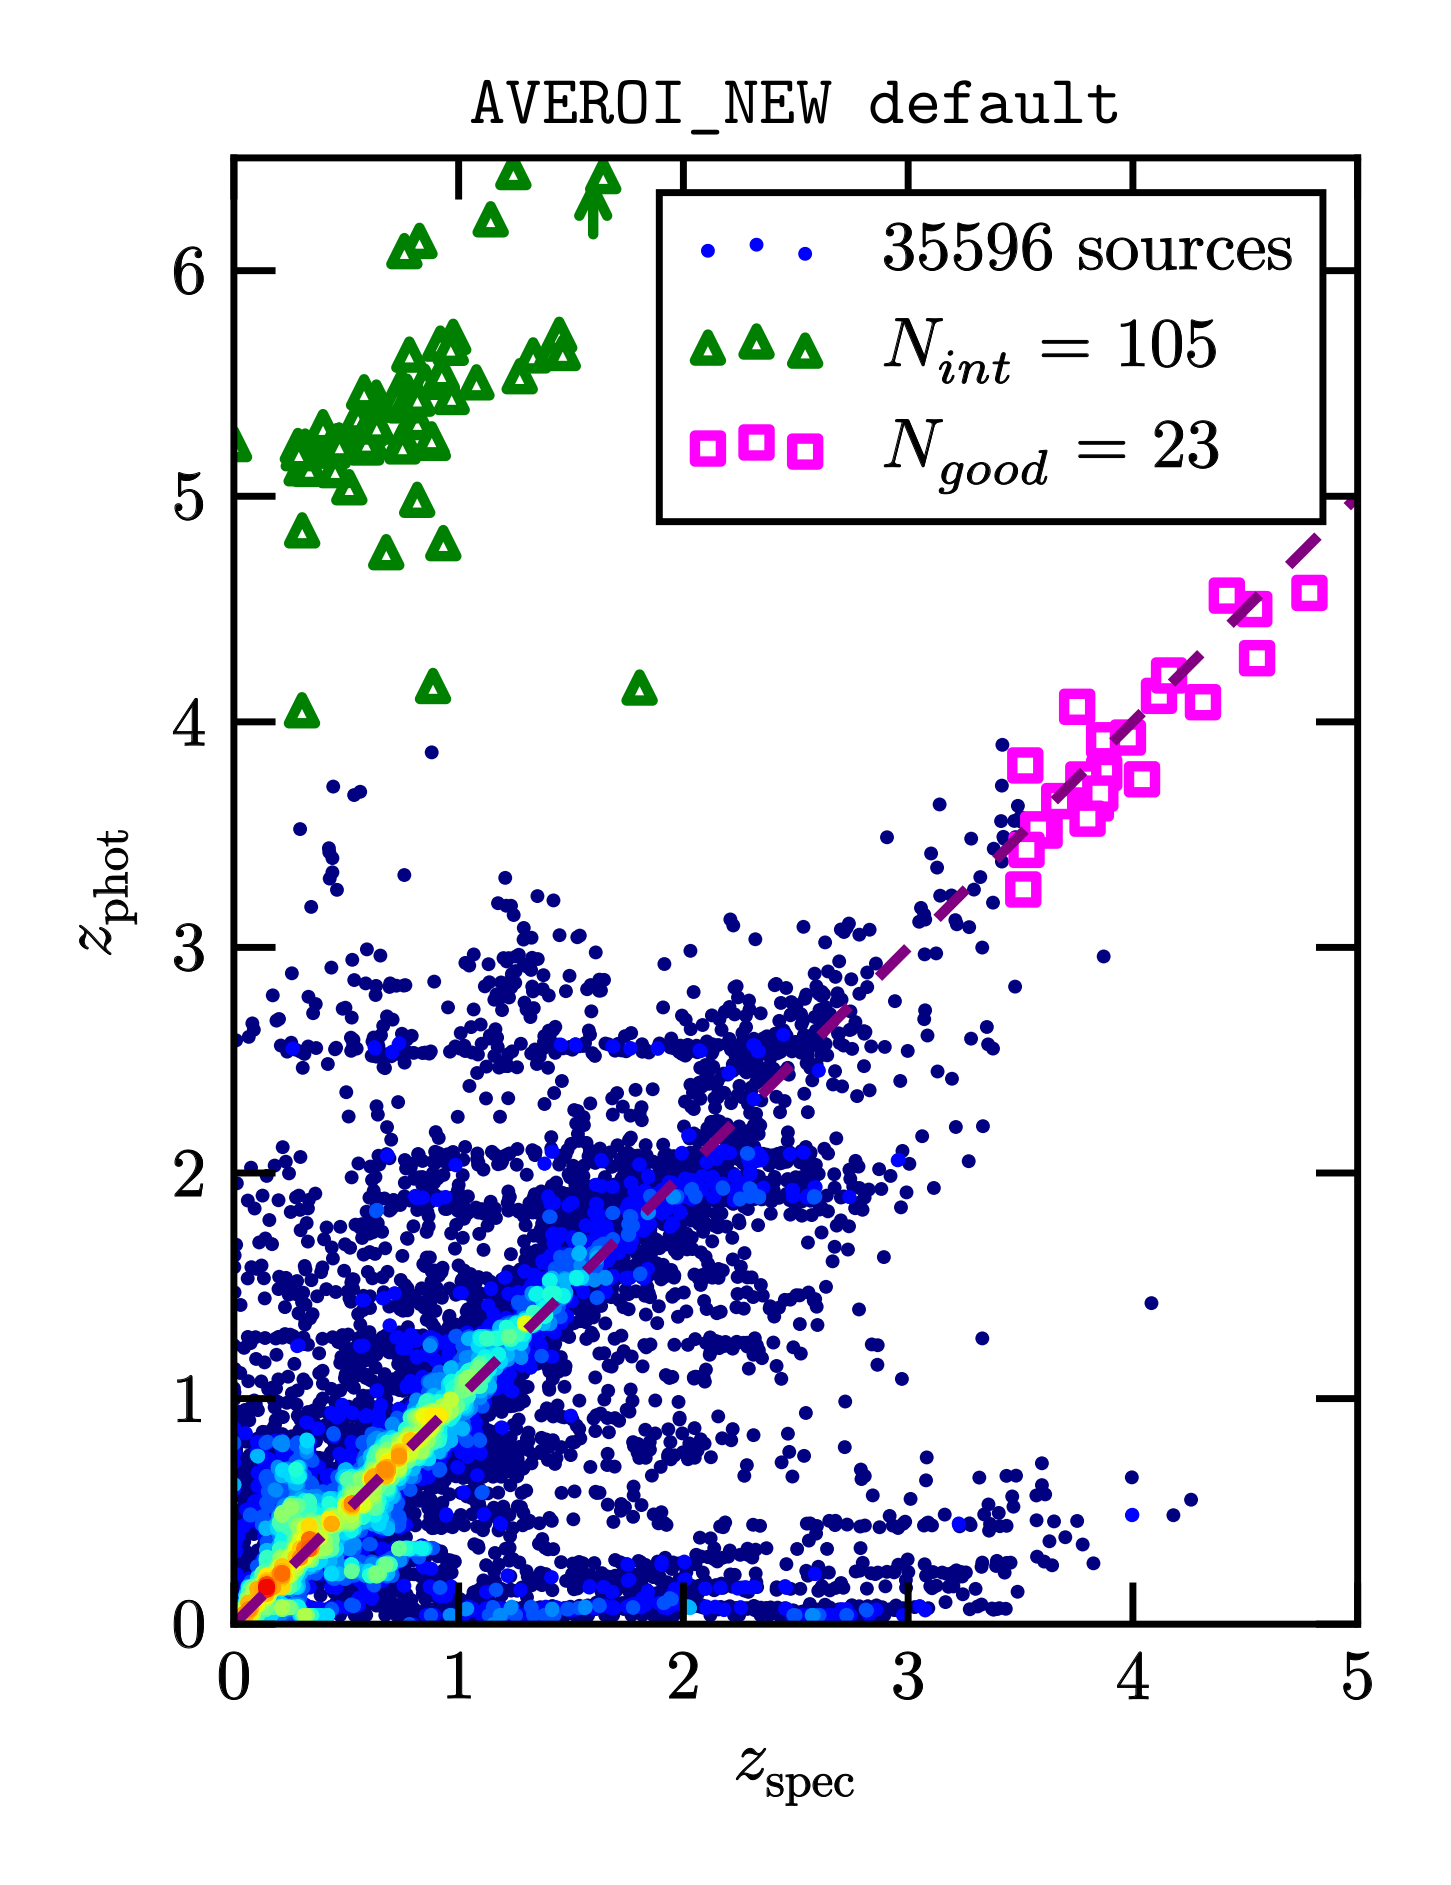
\includegraphics[clip, width=0.5\textwidth]{Chapter3/Figs/template_basic.png}}
\subfloat[\label{fig:cosmos_basic}]{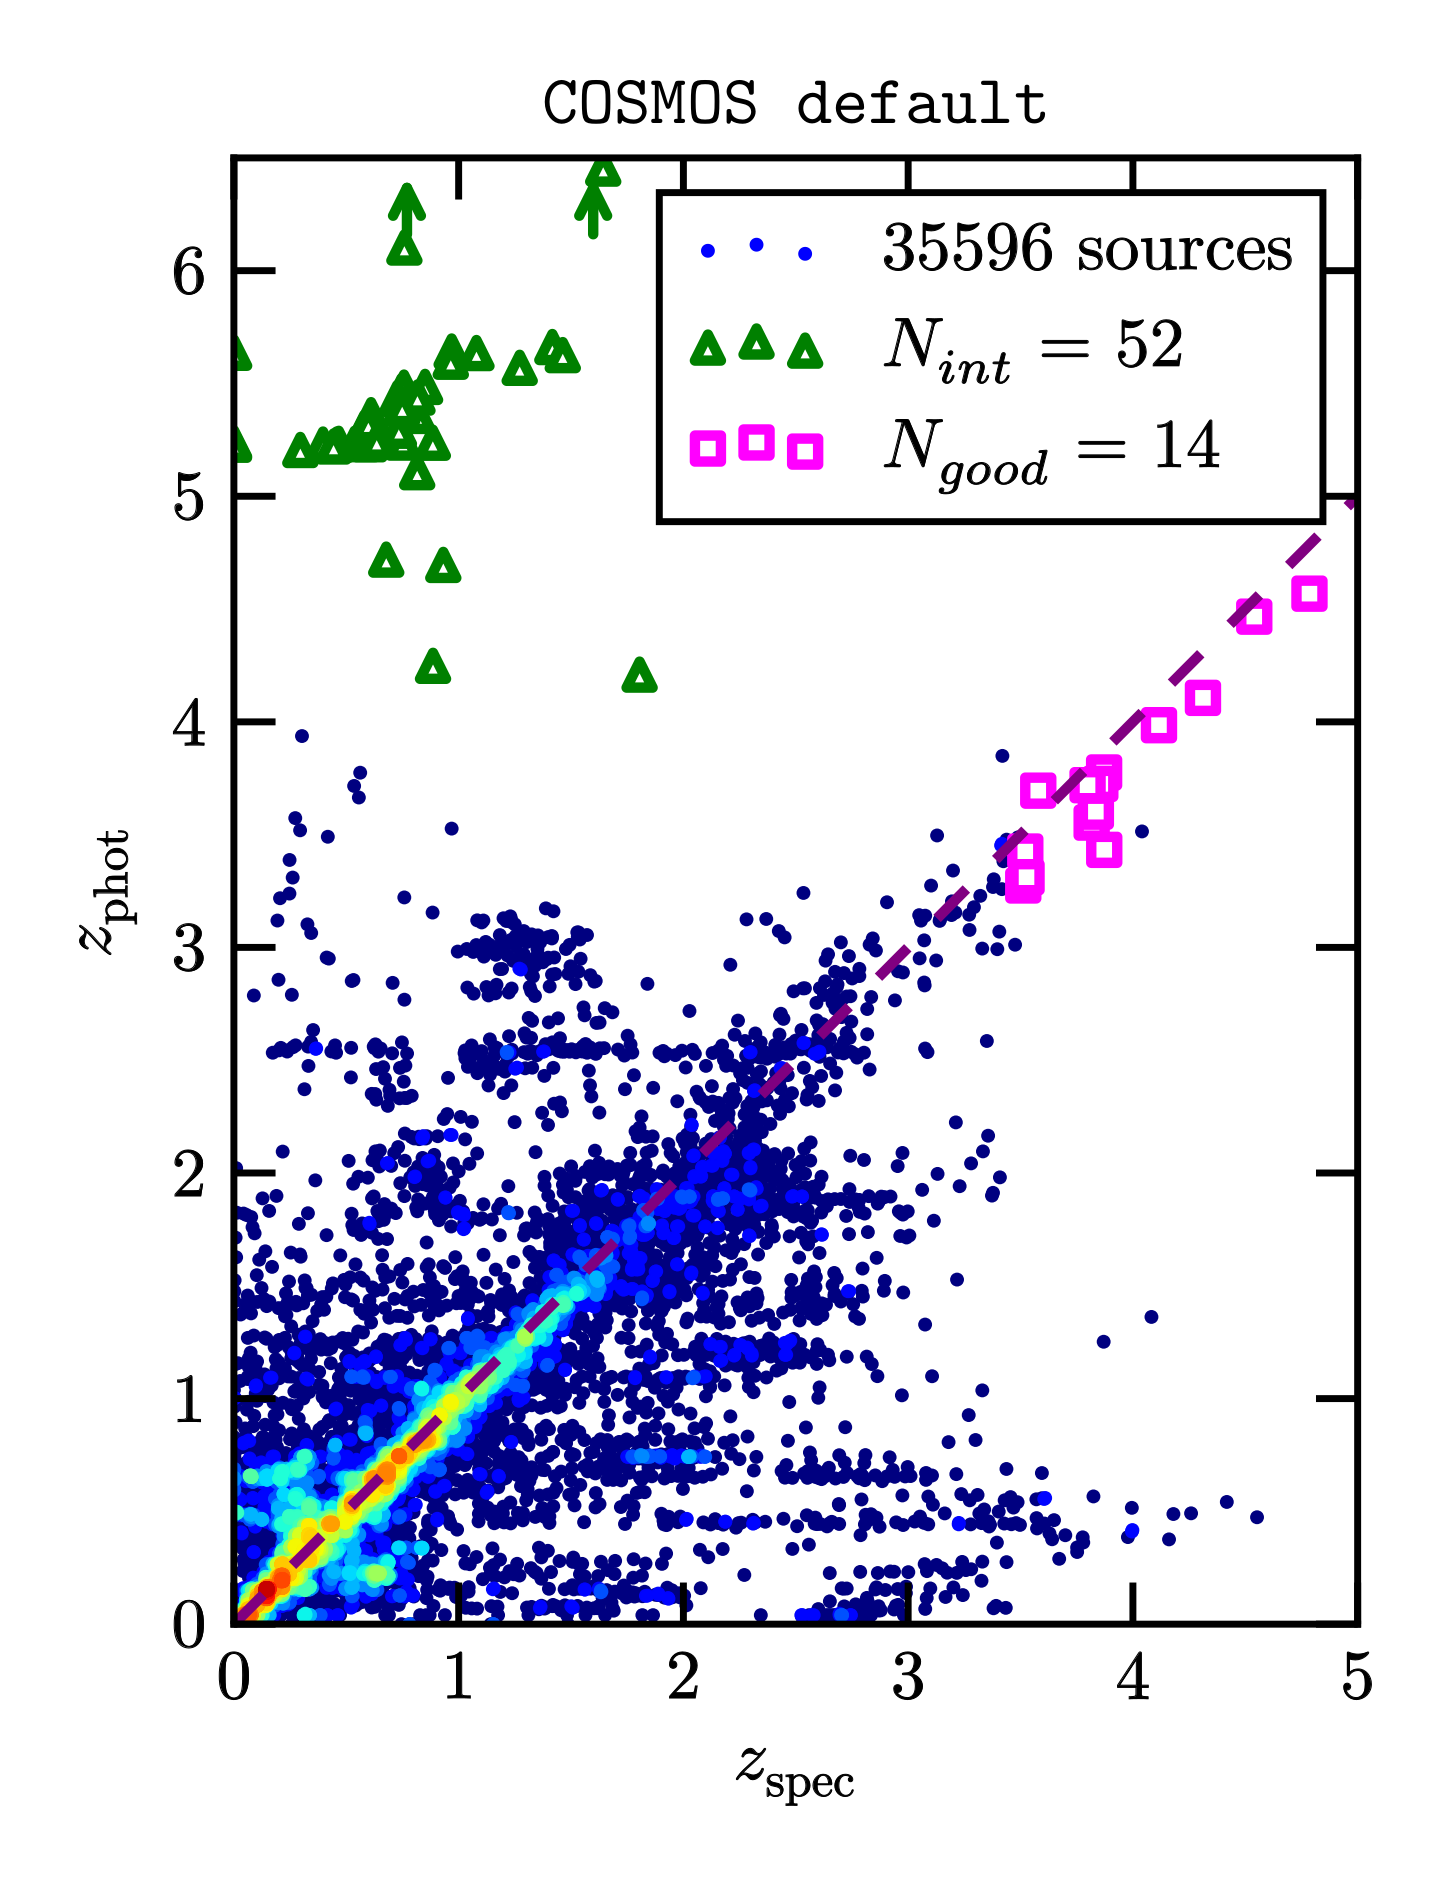
\includegraphics[clip, width=0.5\textwidth]{Chapter3/Figs/template_cosmos.png}}
\caption[\texorpdfstring{$z_{\mathrm{spec}}$}{} vs \texorpdfstring{$z_{\mathrm{phot}}$}{} distributions of the test configurations]{The distribution of spectroscopic vs photometric redshifts for all configurations listed in Table \ref{table:photoz_test}. The colour of each data point shows the number density in bins of 0.01, on a rainbow scale of blue (low) to red (high). The colours have been normalised over all figures, so that the same colour depicts the same number density across all plots. The pink squares represent good high-redshift fits, defined via $N_{\mathrm{good}}$ in Equation \ref{eqn:N_good}. The green triangles show low-redshift interlopers defined via $N_{\mathrm{int}}$ in Equation \ref{eqn:N_int}. The green arrows in some figures indicate interlopers for which the photometric redshift falls outside the plotted window (i.e. $z_{\mathrm{phot}}>6.5$).}\label{fig:photoz_distribution}
\end{figure}

\begin{figure}
\ContinuedFloat
\subfloat[\label{fig:less_ext}]{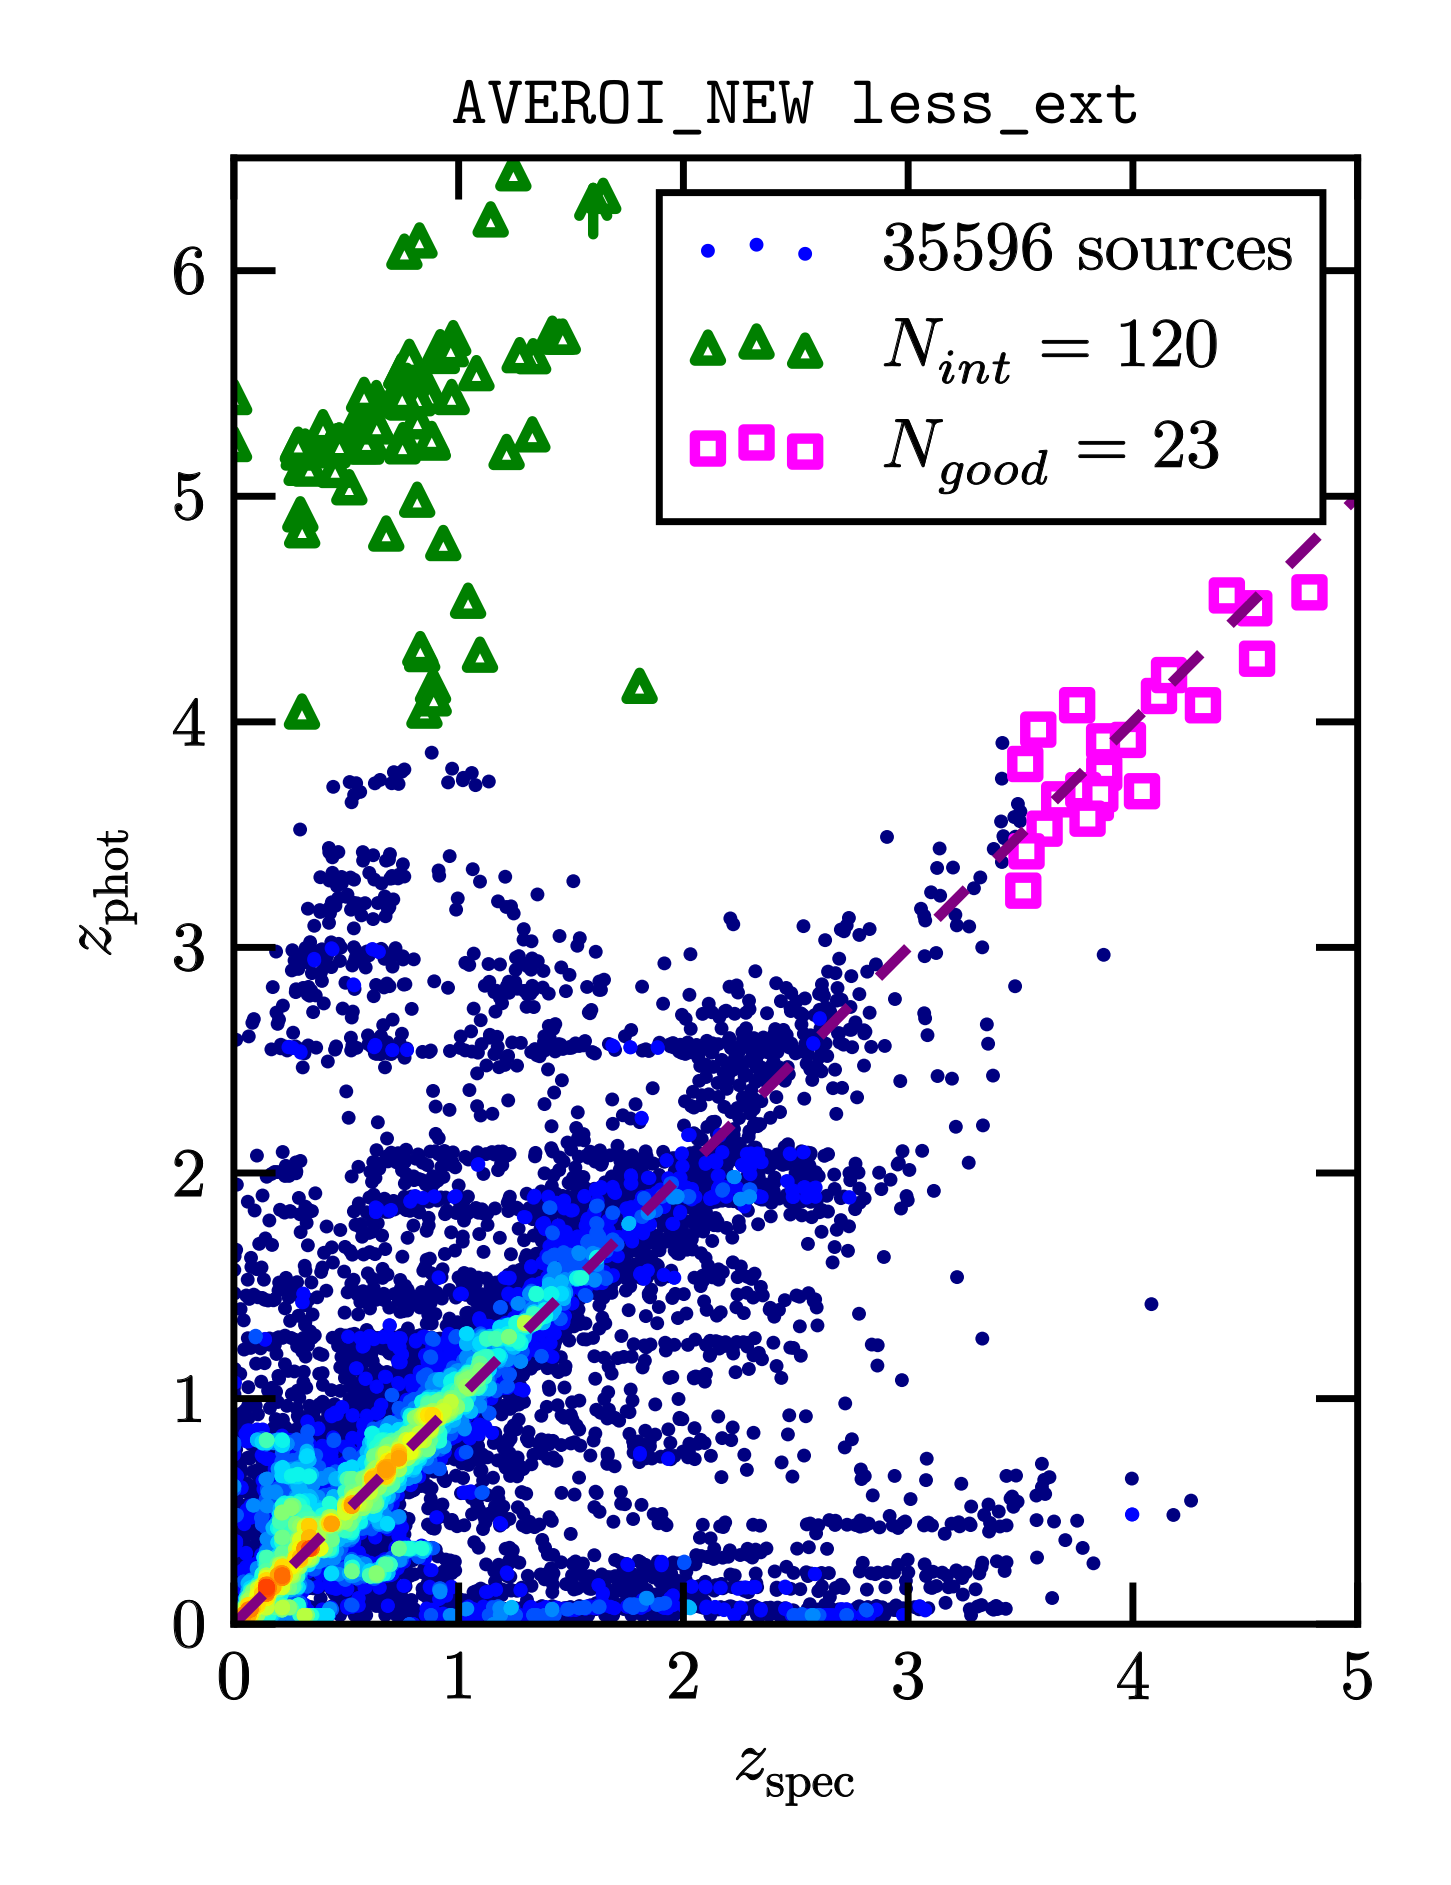
\includegraphics[clip, width=0.5\textwidth]{Chapter3/Figs/template_less_ext.png}}
\subfloat[\label{fig:more_ext}]{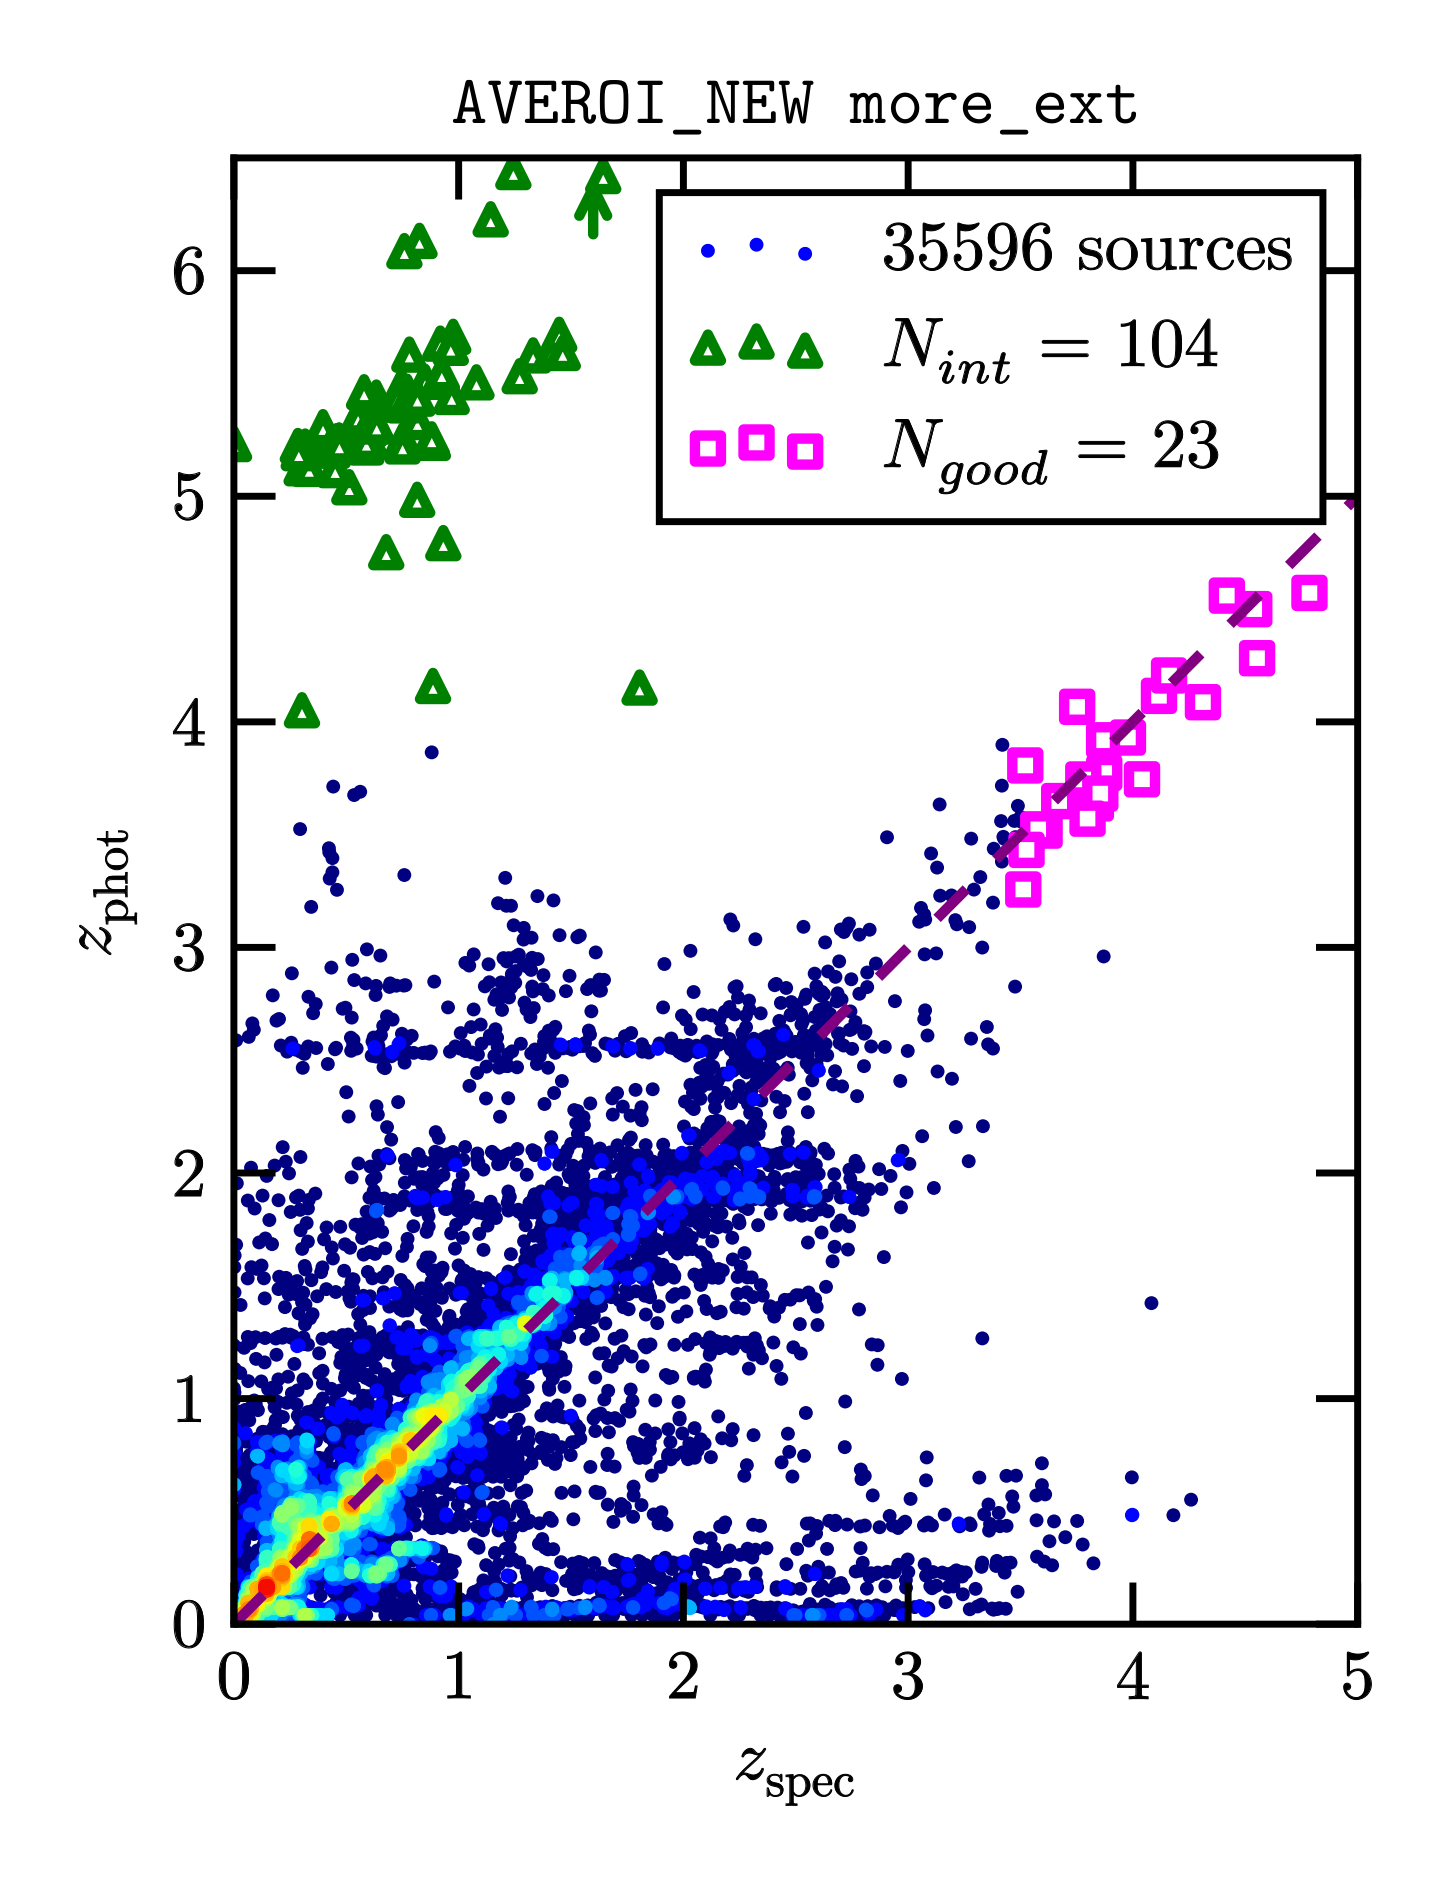
\includegraphics[clip, width=0.5\textwidth]{Chapter3/Figs/template_more_ext.png}}

\subfloat[]{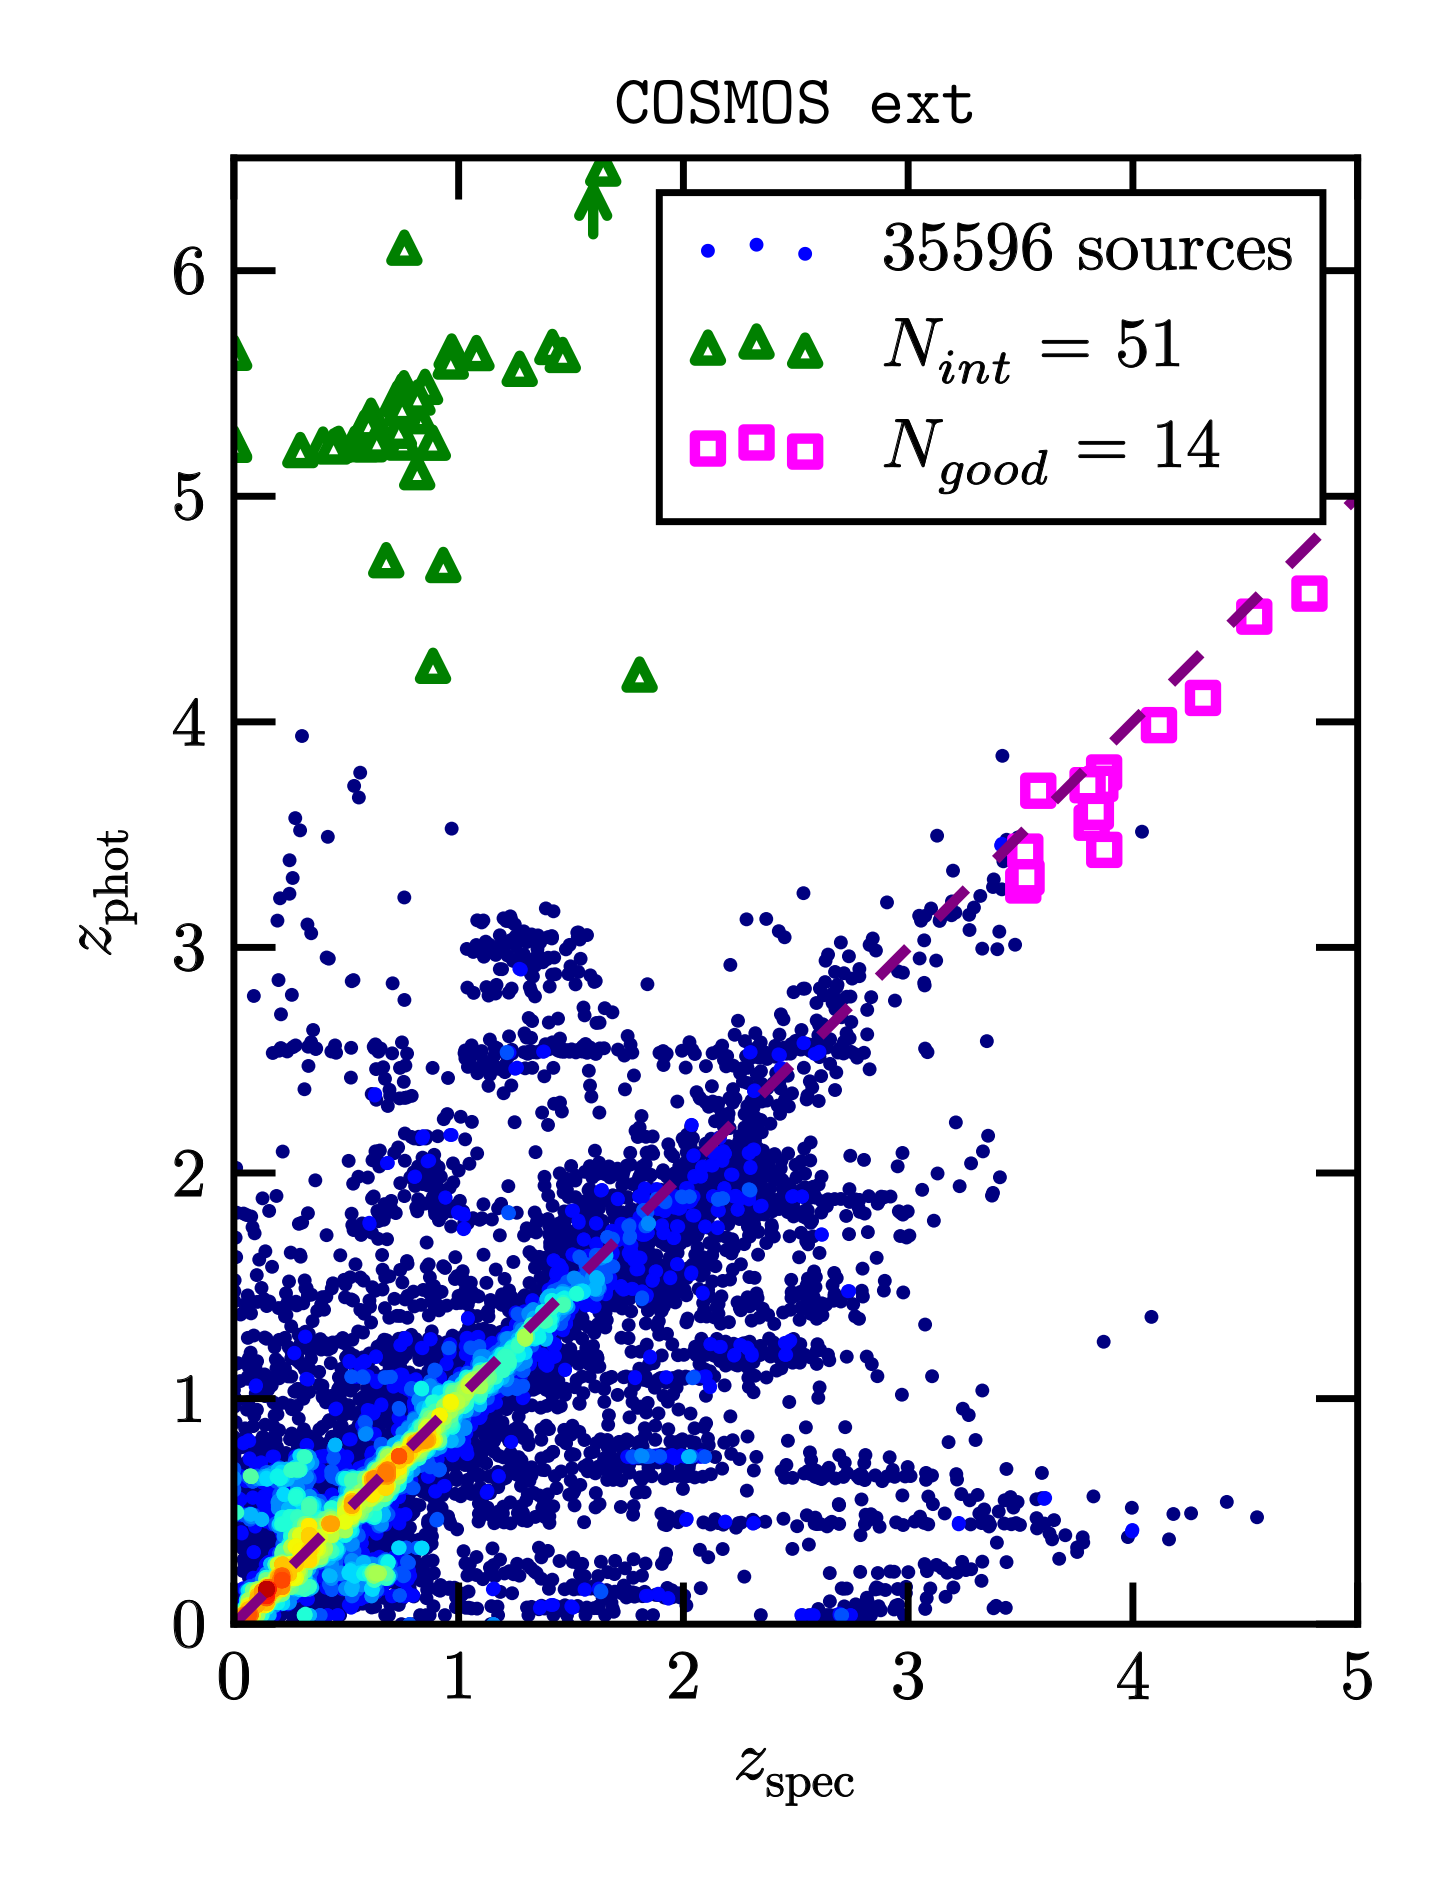
\includegraphics[clip, width=0.5\textwidth]{Chapter3/Figs/template_cosmos_ext.png}}
\subfloat[]{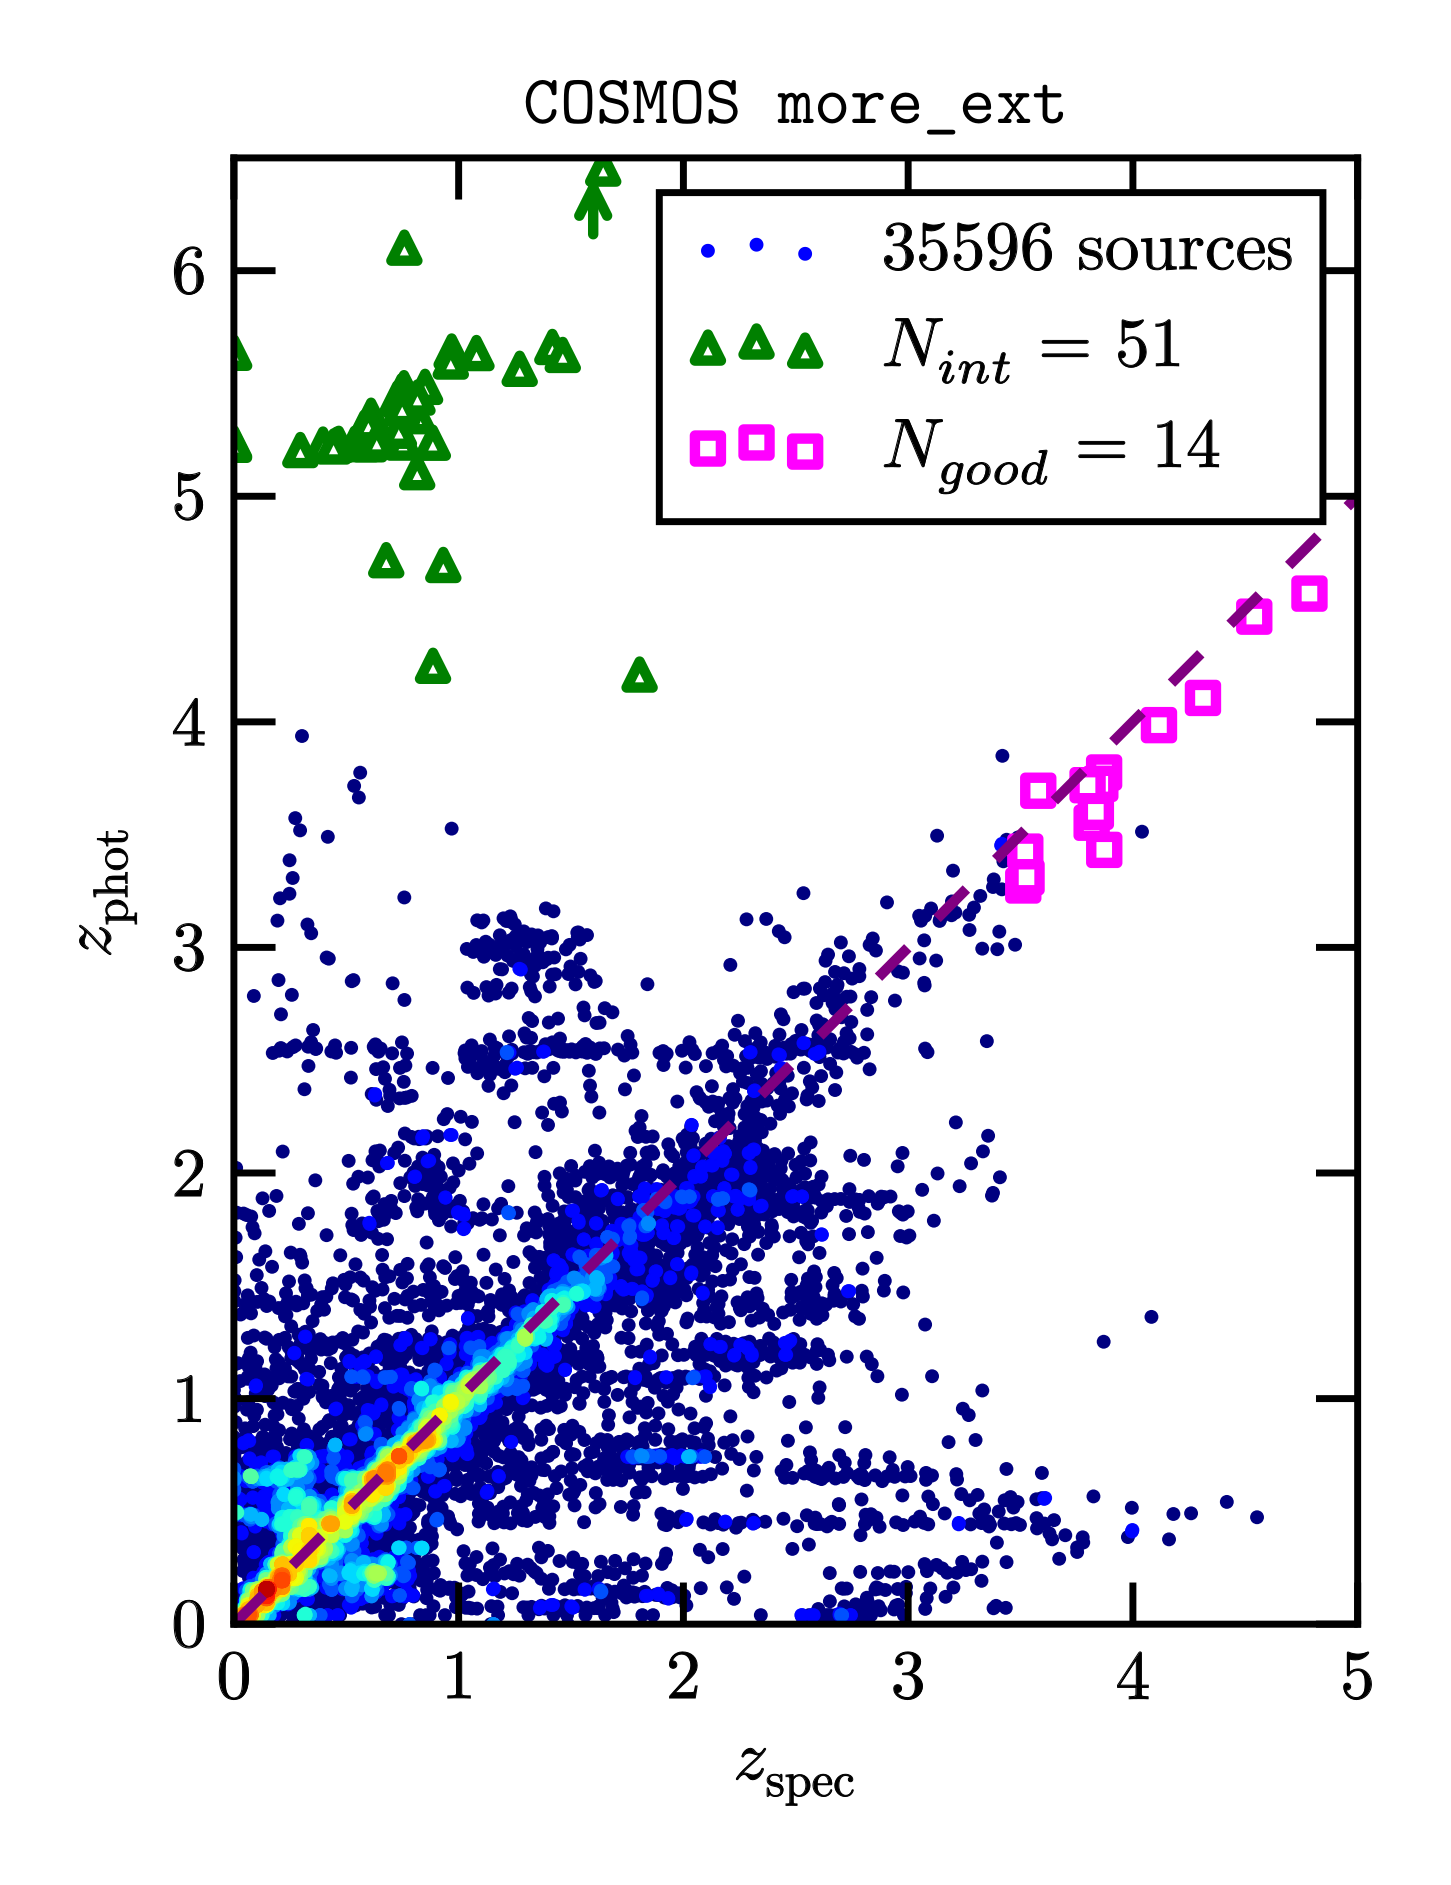
\includegraphics[clip, width=0.5\textwidth]{Chapter3/Figs/template_cosmos_more_ext.png}}
\caption{\textit{continued}}
\end{figure}

\begin{figure}
\ContinuedFloat
\subfloat[\label{fig:no_emlines}]{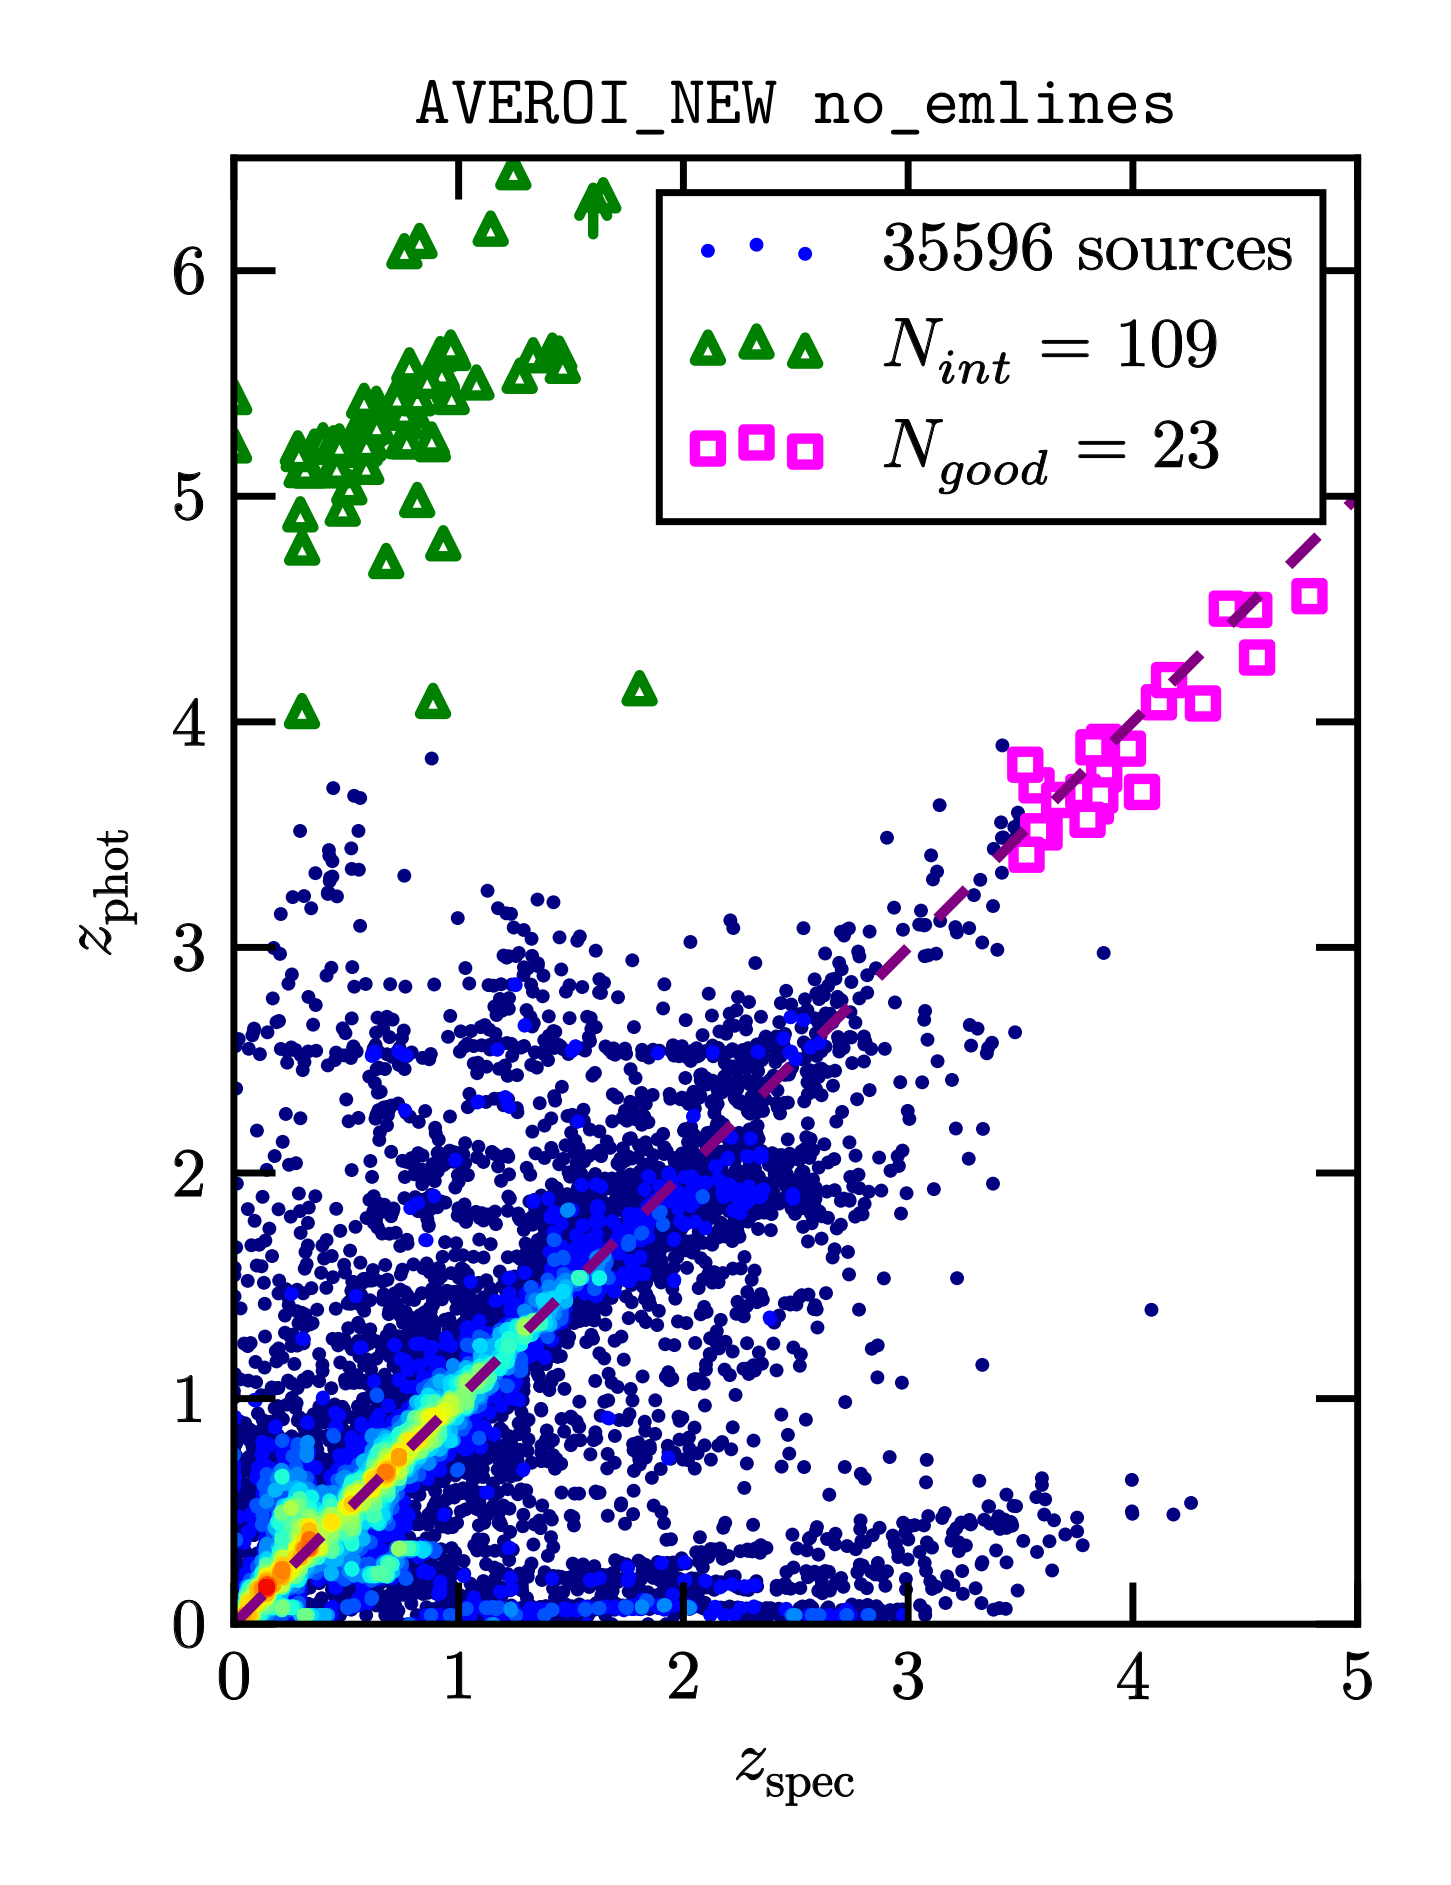
\includegraphics[clip, width=0.5\textwidth]{Chapter3/Figs/template_no_emlines.png}}
\subfloat[\label{fig:cosmos_no_emlines}]{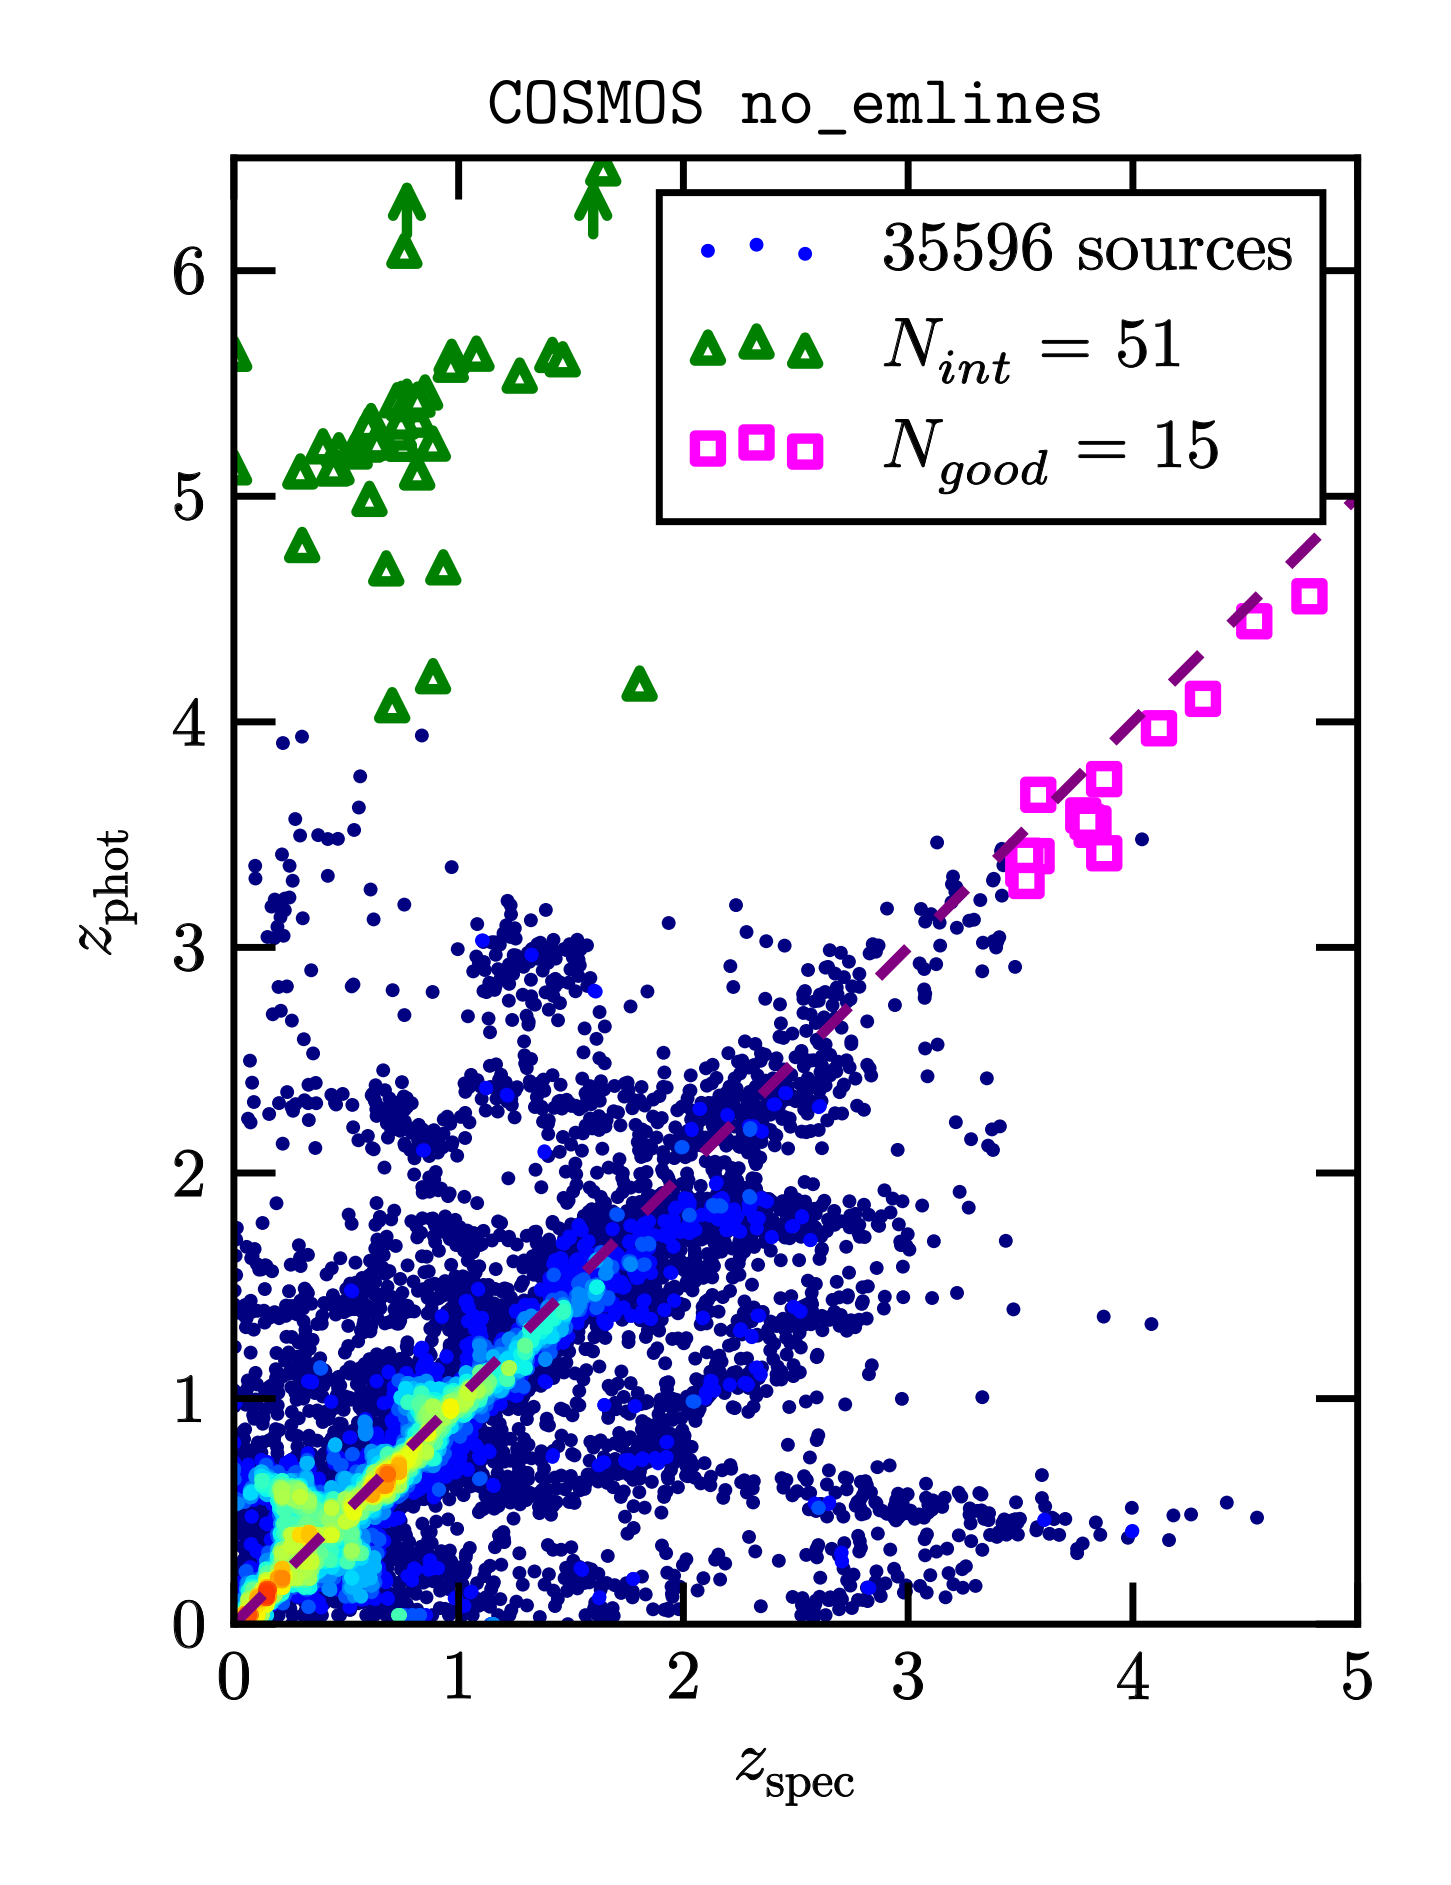
\includegraphics[clip, width=0.5\textwidth]{Chapter3/Figs/template_cosmos_no_emlines.png}}

\subfloat[\label{fig:no_prior}]{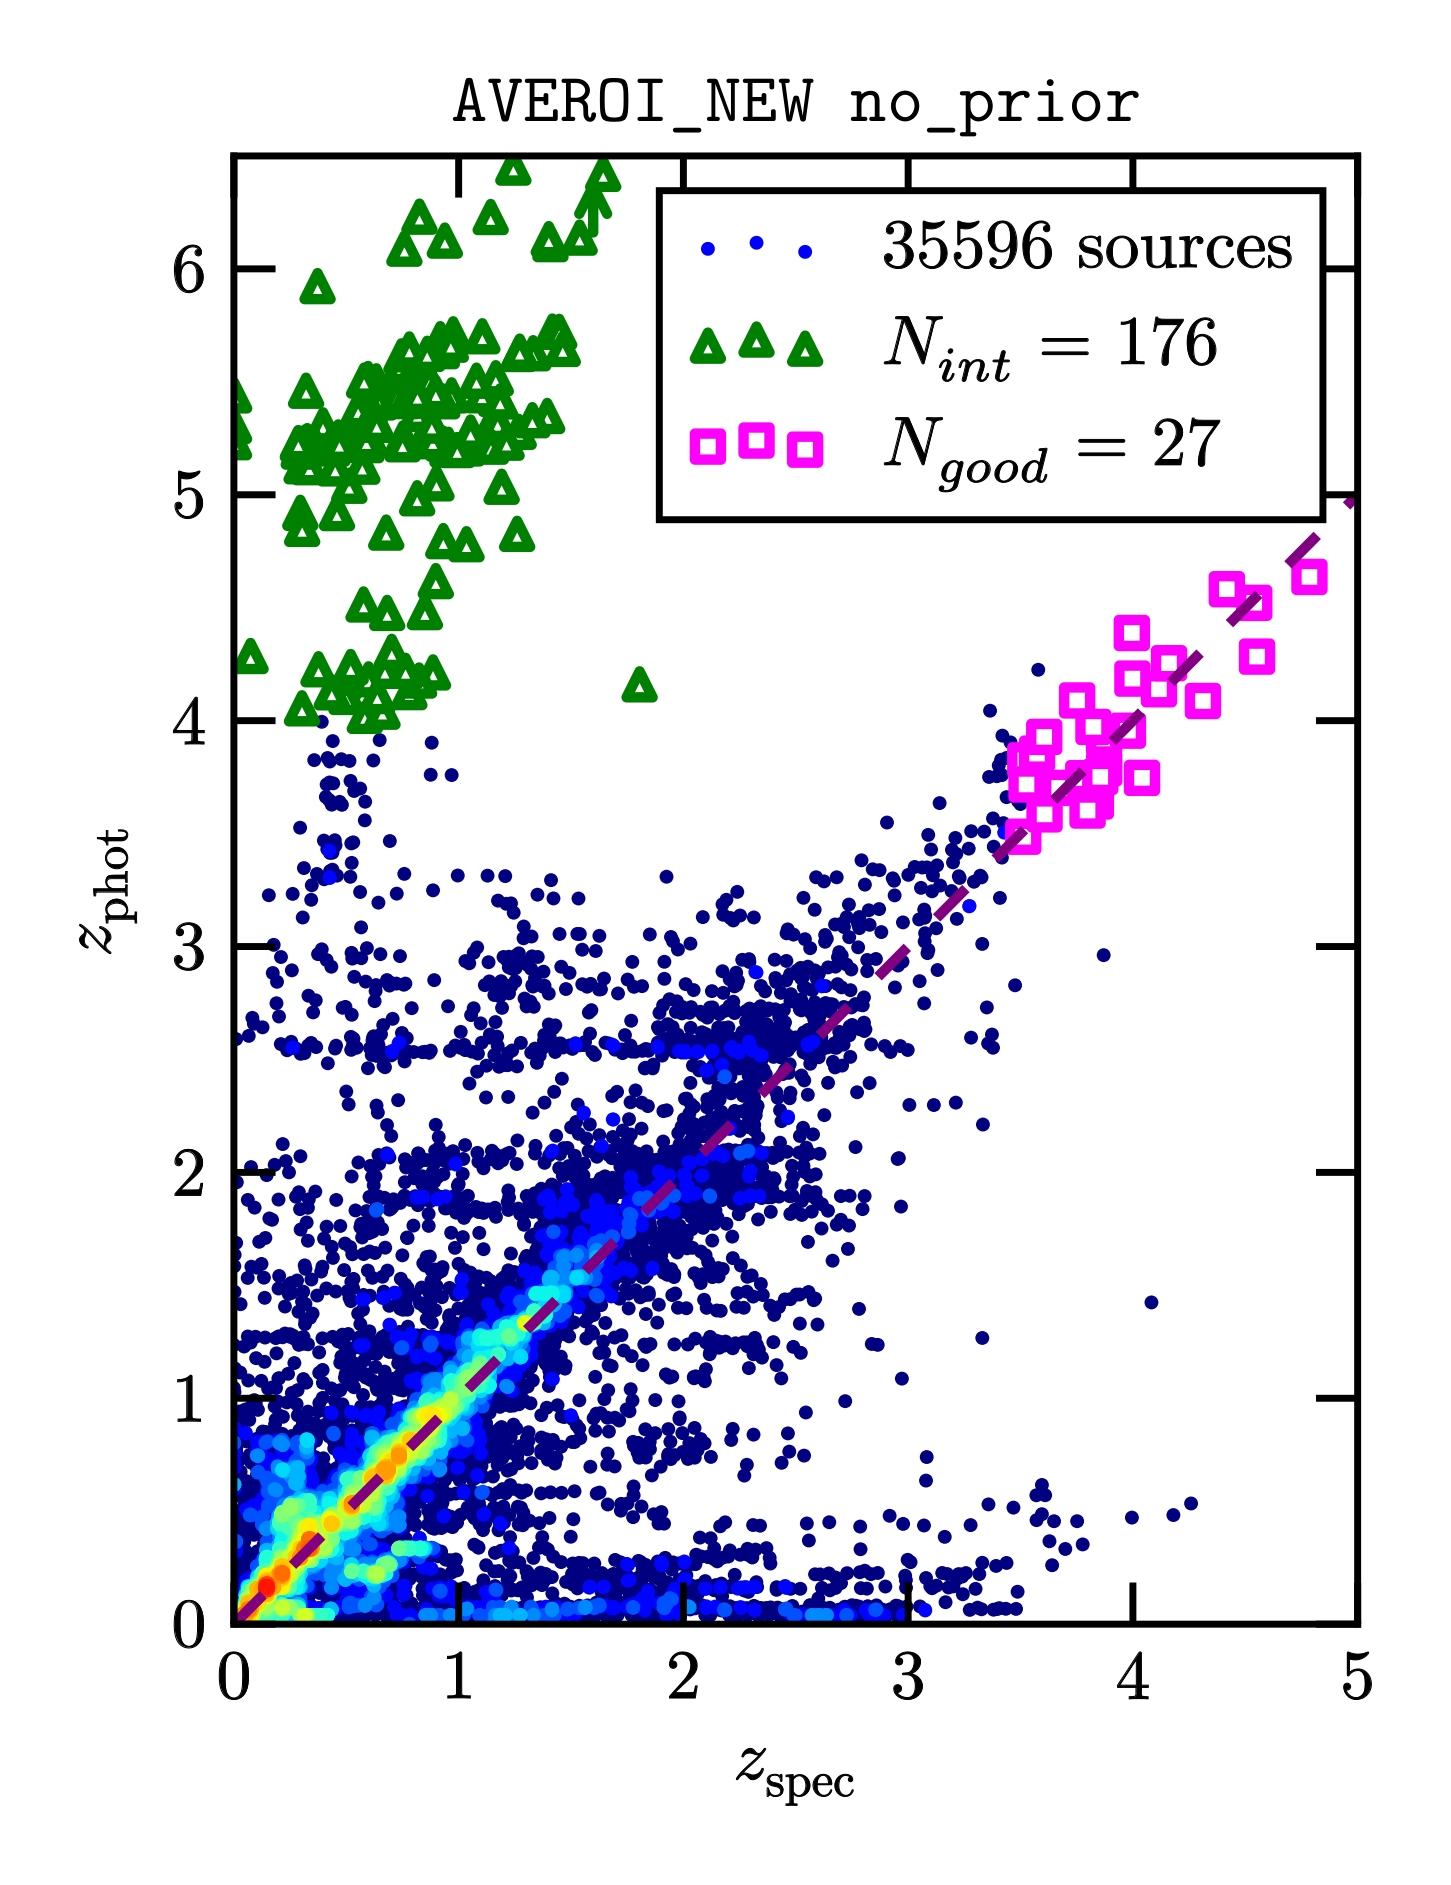
\includegraphics[clip, width=0.5\textwidth]{Chapter3/Figs/template_no_prior.png}}
\subfloat[\label{fig:cosmos_no_prior}]{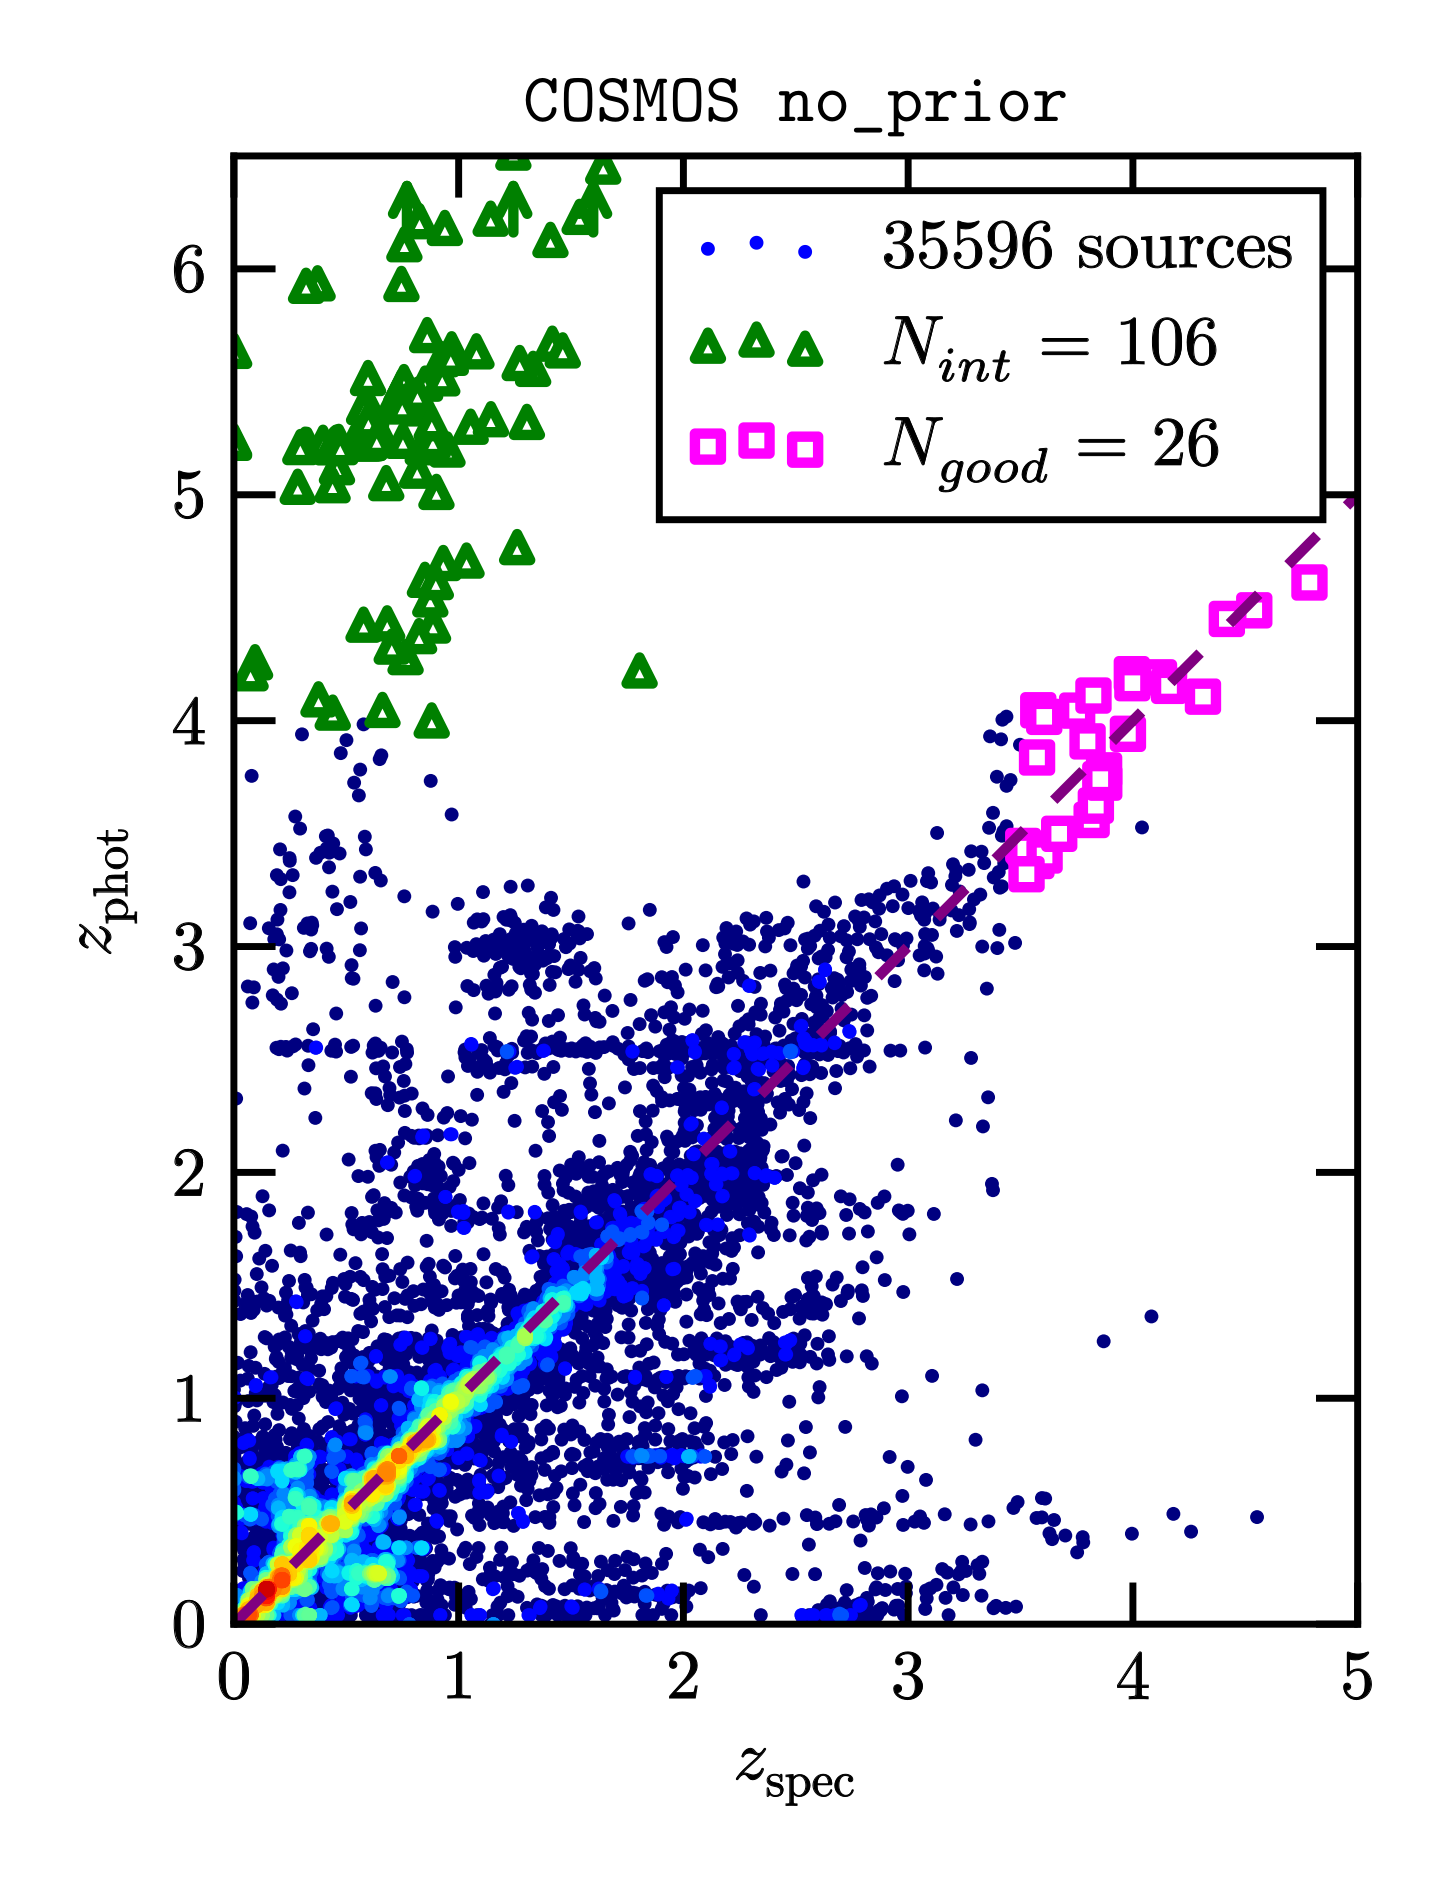
\includegraphics[clip, width=0.5\textwidth]{Chapter3/Figs/template_cosmos_no_prior.png}}
\caption{\textit{continued}}
\end{figure}

\begin{figure}
\ContinuedFloat
\subfloat[]{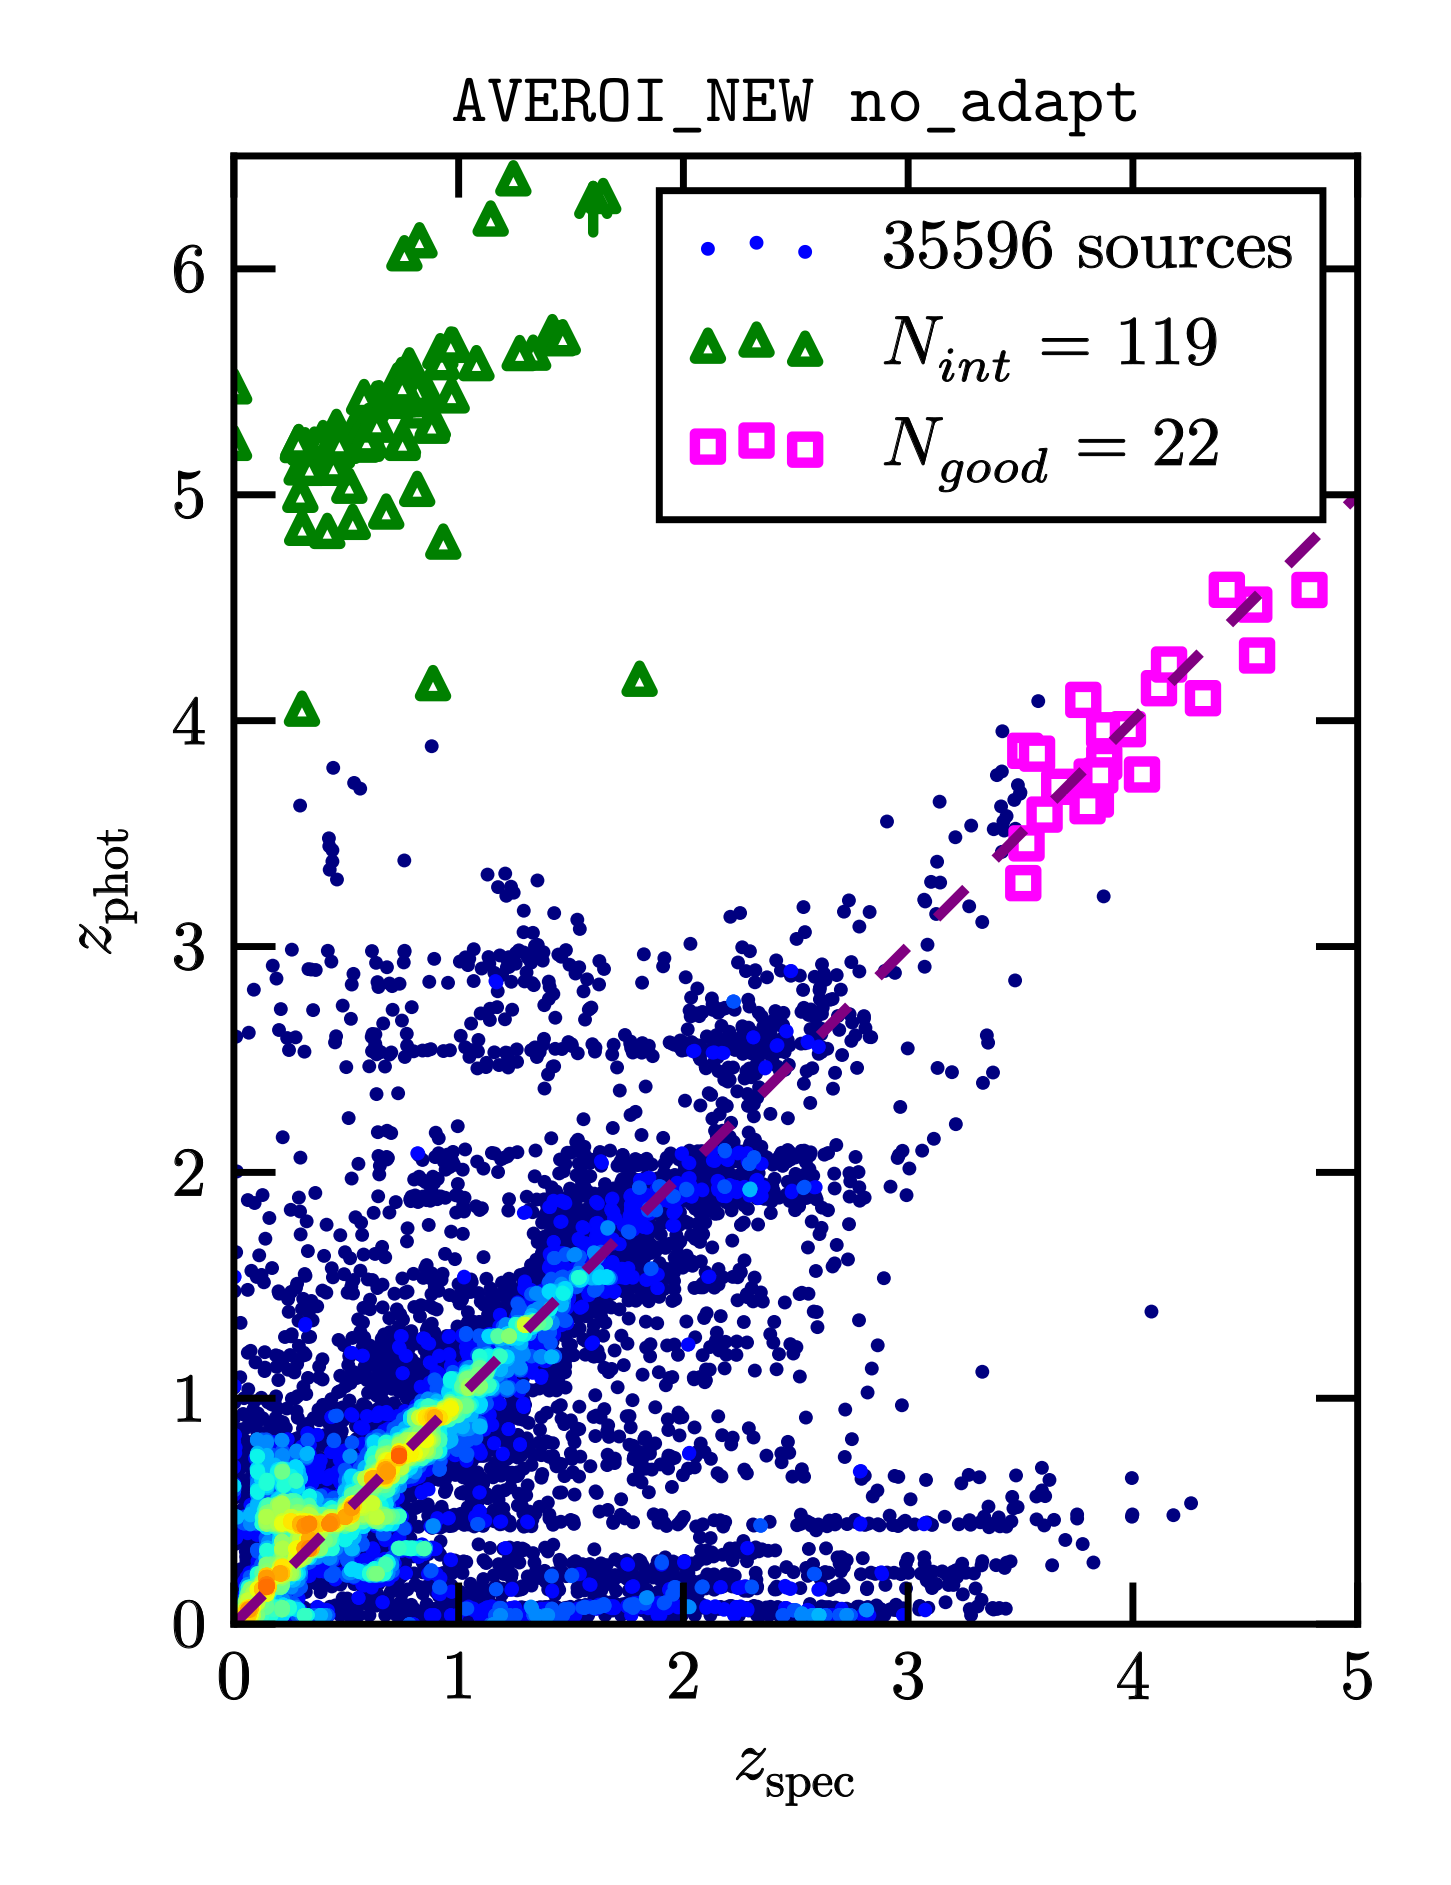
\includegraphics[clip, width=0.5\textwidth]{Chapter3/Figs/template_no_adapt.png}}
\subfloat[\label{fig:cosmos_no_adapt}]{\includegraphics[clip, width=0.5\textwidth]{Chapter3/Figs/template_cosmos_no_adapt.png}}

\subfloat[]{\includegraphics[clip, width=0.5\textwidth]{Chapter3/Figs/template_auto.png}}
\subfloat[]{\includegraphics[clip, width=0.5\textwidth]{Chapter3/Figs/template_cosmos_auto.png}}
\caption{\textit{continued}}
\end{figure}

\begin{figure}
\ContinuedFloat
\subfloat[\label{fig:des_only}]{\includegraphics[clip, width=0.5\textwidth]{Chapter3/Figs/template_des_only.png}}
\subfloat[\label{fig:cosmos_des_only}]{\includegraphics[clip, width=0.5\textwidth]{Chapter3/Figs/template_cosmos_des_only.png}}

\subfloat[]{\includegraphics[clip, width=0.5\textwidth]{Chapter3/Figs/template_des_only_auto.png}}
\subfloat[]{\includegraphics[clip, width=0.5\textwidth]{Chapter3/Figs/template_cosmos_des_only_auto.png}}
\phantomcaption
\end{figure}





\section{Discussion on configuration testing}\label{section:photoz_discussion}
The part of this chapter concerned with photometric redshift testing has now reached its final stage, where the preceding results can be used to explore the effect of all the different options that have been trialled. To this end, the current section will present a comparative evaluation of the photometric redshift performance for all the setups. In the analysis, configurations are compared by the values of their accuracy metrics in Table \ref{table:photoz_test} and by their photo-z distributions in Figure \ref{fig:photoz_distribution}. \par 

The end goal is to find the most suitable way to estimate photo-zs for the \DESVIDEO catalogue, which, as emphasised throughout this thesis, needs to be specifically geared towards optimal results at high redshifts.  At several points the discussion will also comment on the implication of the test results for general photo-z research. These analyses will disregard the high-redshift accuracy metrics, and looks only at those statistics that apply to the full testing sample --- i.e. the bias, scatter, and outlier fractions. Those primarily reflect the accuracy for the low-redshift ($z_{\mathrm{spec}}\lesssim1.5$) majority of galaxies in the sample, which is also approximately the range that most other photo-z studies tend to focus on.\par

%LOOK AT THIS TEXT BELOW
%As Section \ref{subsection:conclusion_photoz_intro} indicated at the start, one of the aims of this thesis is to utilise the \DESVIDEO dataset to investigate photo-z optimisation for the sake of future studies. Section \ref{section:photoz_discussion} has therefore analysed the general implications of the \DESVIDEO tests. This investigation looked only at the bias, scatter, and outlier fraction metrics, i.e. those that were measured on all objects in the testing sample. Naturally, these metrics thus primarily reflect the accuracy for the low-redshift ($z_{\mathrm{spec}}\lesssim1.5$) majority of galaxies in the sample, which is also the range at which most photo-z studies operate.



\subsection{Templates}
\subsubsection{Template sets}\label{subsubsection:template_sets}
In order to investigate which template set performs best, the \texttt{AVEROI\_NEW} and \texttt{COSMOS} entries in Table \ref{table:photoz_test} are compared directly for each setup\footnote{The \texttt{AVEROI\_NEW} \texttt{less\_ext} and \texttt{COSMOS} \texttt{ext} configurations are not directly comparable, because they use very different amounts of extinction. Therefore they are not considered in this template set comparison.}. A general observation is that the \texttt{COSMOS} templates perform better than the \texttt{AVEROI\_NEW} templates for most statistical measures and most configurations. The \DESVIDEO tests thus confirm the claim by \cite{2009ApJ...690.1236I} mentioned earlier in Section \ref{subsubsection:COSMOS}, that the \texttt{COSMOS} SEDs are generally more accurate than template sets based on the CWW spectra (such as the \texttt{AVEROI\_NEW} SEDs). \par


In terms of metrics, a notable exception is that the \texttt{AVEROI\_NEW} templates consistently show a larger value for $N_{\mathrm{good}}$ (except in the \texttt{des\_auto} setup where the values are identical). Secondly, the \texttt{AVEROI\_NEW} templates also perform better in terms of mean bias $\overbar{\Delta z}$ in all but one case (the \texttt{no\_prior} configuration being the exception). Regarding configurations, there are two instances where the \texttt{AVEROI\_NEW} templates are conclusively more accurate than \texttt{COSMOS}, namely the \texttt{des} and \texttt{des\_auto} setups. For the \texttt{des} setup, the mean and median bias $\overbar{\Delta z}$ and $\Delta z_{50}$ are 0.0120 and 0.0057 lower for the \texttt{AVEROI\_NEW} templates, and the $\sigma $, $f_{2\sigma}$, and $f_{3\sigma}$ values are 10.2\%, 13.7\% and 13.9\% lower. For the \texttt{des\_auto} configuration the metrics are lower by 0.0319 and 0.0242 for $\overbar{\Delta z}$ and $\Delta z_{50}$, and 13.2\%, 10.5\% and 16.4\% for $\sigma$, $f_{2\sigma}$ and $f_{3\sigma}$. A possible explanation for why the \texttt{AVEROI\_NEW} templates perform slightly better when using exclusively optical data might be found within Section \ref{subsubsection:COSMOS}. To recap, there it was stated that \cite{2009ApJ...690.1236I} claim that the better accuracy of the \texttt{COSMOS} templates is because they produce a better joining of the UV to the infrared. If this is indeed the reason why these SEDs perform better for the full \DESVIDEO filterset, it would follow that this advantage would not apply when only optical data is used. At the same time, the \texttt{AVEROI\_NEW} templates might be more reliable over visible wavelengths because that part of these spectra is based on the empirically measured CWW SEDs, whereas the \texttt{COSMOS} SEDs are theoretical. Furthermore, the CWW spectra are local, and the spectroscopic dataset used for the statistics is predominantly low-redshift. \par

Let us now return to the observation that the \texttt{COSMOS} templates generate superior statistics on the whole. Particularly interesting is the discovery that the \texttt{default} \texttt{COSMOS} setup produces better results than the \texttt{more\_ext} \texttt{AVEROI\_NEW} setup. Over the course of the following few sections, it will be demonstrated that those two are the best choice for their respective template sets. Upon comparing these configurations, the \texttt{COSMOS} metrics come out 0.0055 lower for $\Delta z_{50}$, and lower by 16.1\% in $\sigma$, 23.7 \% in $\sigma_{68}$, 0.8\% in $f_{2\sigma}$, and 10.2\% in $f_{3\sigma}$. The number of low-redshift interlopers $N_{\mathrm{int}}$ is also twice as small. The only instances where the \texttt{more\_ext} \texttt{AVEROI\_NEW} templates perform better is with regard to the mean bias $\overbar{\Delta z}$ (lower by 0.016), and the number of successfully retrieved high-redshift objects $N_{\mathrm{good}}$: the \texttt{COSMOS} setup correctly identifies only 14 high-redshift galaxies, whereas the \texttt{AVEROI\_NEW} results find 23. In the end, the latter advantage is one of the major reasons why the high-redshift search later in this thesis makes use of the \texttt{AVEROI\_NEW} templates. Section \ref{subsection:template_choice} will describe the reasons for this choice in detail. \par

The remainder of the setup comparisons will now determine the best configuration parameters for each template set. Such an analysis is useful both for finding the best way to apply each template set, and for a template-independent assessment of all the parameter options. The topic of template set choice will be revisited at the end in Section \ref{subsubsection:templates_revisited}.\par %TEMPLATE-INDEPENDENT COMPARISONS




\subsubsection{Extinction}\label{subsubsection:extinction_discussion}
The next point of inquiry involves the effects of dust extinction on the photo-zs. The observed trends with various amounts of extinction differ between the two template sets. To start with, the discussion will focus on the \texttt{AVEROI\_NEW} templates. It is evident from Table \ref{table:photoz_test} that the \texttt{default} setup with extinction values of up to $E(B-V)=1.0$ performs better than the \texttt{less\_ext} setup with a maximum extinction of only $E(B-V)=0.3$ (recommended in the \texttt{LePHARE} installation). The superior performance is demonstrated across $\overbar{\Delta z}$ (better by 0.0197), $\Delta z_{50}$ (0.0003), $\sigma$ (better by 9.0\%), $\sigma_{68}$ (10.3\%), $f_{2\sigma}$ (6.3\%), $f_{3\sigma}$ (9.0\%) and $N_{\mathrm{good}}$ (16 fewer interlopers). $N_{\mathrm{int}}$ is the only statistic where both setups are equally accurate. Specific reasons for this improvement can be found in Figure \ref{fig:basic} and Figure \ref{fig:less_ext}. The latter plot demonstrates that the \texttt{less\_ext} configuration contains a population of galaxies at $0\lesssim z_{\mathrm{spec}} \lesssim 1.5$ that are assigned high photo-zs of $z_{\mathrm{phot}}\gtrsim 2.5$. When inspecting the imaging and photometry for these sources, it becomes apparent that they are extremely red galaxies. It is likely that they are so red that without templates with adequate dust extinction the \SI{4000}{\angstrom} break at $z<1.5$ is mistaken for a \SI{1216}{\angstrom} Lyman break at $z>2.5$. However, when higher extinction values are included through the \texttt{default} setup, these galaxies are fitted well. The findings above thus suggest that the $E(B-V)\leq0.3$ dust extinction values listed in the \texttt{LePHARE} installation do not span the full range of attenuation observed in real galaxies. In fact, this shortcoming was partly implicitly acknowledged by the \cite{2007A&A...476..137A} study that the \texttt{AVEROI\_NEW} templates are derived from, which includes $E(B-V)$ values of up to 0.6. Nonetheless, the \DESVIDEO results indicate that this is also not sufficient --- out of a sample of 166 $z_{\mathrm{phot}}\gtrsim 2.5$ interloper galaxies that are poorly fitted by the \texttt{less\_ext} exctinction range, 16 are best fitted by templates as red as $E(B-V)=1.0$. This number is of the same order as the number of true high-redshift objects $N_{\mathrm{good}}=24$. This thesis therefore emphasises that it is important for high-redshift studies to include templates with large amounts of extinction, in order to accurately model very attenuated sources.\par 


%\begin{figure*}[!htpb]
%\centering
%\subfloat[]{
%	\includegraphics[clip, width=0.50\textwidth]{Chapter3/Figs/difference_basic.png}}
%\subfloat[]{
%	\includegraphics[clip, width=0.50\textwidth]{Chapter3/Figs/difference_less_ext.png}}
%\caption[]{}
%\label{fig:ext_difference}
%\end{figure*}


The \texttt{more\_ext} configuration is aimed at testing whether extinction values above $E(B-V)=1.0$ would further improve the photo-zs. Table \ref{table:photoz_test} shows that this is not the case for the spectroscopic testing sample, as the difference between the \texttt{default} and \texttt{more\_ext} metrics is negligible (the \texttt{default} results show only a marginal 0.0004 lower $\overbar{\Delta z}$, and any improvements are at the subpercent level for the $\sigma$, $\sigma_{68}$, $f_{2\sigma}$ and $f_{3\sigma}$ metrics). In fact, only 10 out of \num{35596} sources differed by more than 0.2 in photometric redshift across the two configurations. The two configurations could therefore be considered equivalent for the (low-redshift) population that dominates the spectroscopic subsample. Nevertheless, there is a potential benefit to including redder templates for the high-redshift search in the full catalogue, since extremely red galaxies are a common contaminant. As the statistical metrics indicate that there is no worsening performance when using the \texttt{more\_ext} setup, this potential advantage was considered a sufficient reason to regard the extinction values in the \texttt{more\_ext} as the optimal choice for the \DESVIDEO catalogue. \par 


The remaining analysis of the most suitable extinction values will now focus on the \texttt{COSMOS} templates.  When looking at the results for the \texttt{default} [$E(B-V)\leq0.5$], \texttt{ext} [$E(B-V)\leq1.0$] and \texttt{more\_ext} [$E(B-V)\leq2.0$] configurations, the conclusion is fairly straightforward: the photo-z metrics tend to worsen slightly with increased extinction ($\sigma$ and $f_{3\sigma}$ being the only exceptions). Overall this makes the extinction in the \texttt{default} setup the best choice for the \DESVIDEO data, although it must be noted that the differences between the three configurations are quite small ($<2\%$ for all metrics). The fact that the \texttt{default} setup performs best suggests that the extinction values of $E(B-V)\leq0.5$ in the default setup are largely sufficient, corroborating the values from \cite{2009ApJ...690.1236I} and the \texttt{LePHARE} \texttt{README} files. The optimal dust extinction required for the \texttt{COSMOS} SEDs is therefore less than for the \texttt{AVEROI\_NEW} templates, where values of up to $E(B-V)\leq1.0$ are needed to achieve the best performance. A likely explanation is that the \texttt{COSMOS} template set is either more complete or more accurate at the red end. In the latter case, this could again be related to the fact that the \texttt{COSMOS} templates provide a better joining of the UV to the IR than the \texttt{AVEROI\_NEW} templates, which leads to more accurate red SEDs. \par 


\subsubsection{Emission lines}\label{subsubsection:discussion_emlines}
%THE MOST PROMINENT RESULT IS THAT THERE ARE 4 MORE LOW REDSHIFT INTERLOPERS
To investigate the effect of adding emission lines, the metrics for the \texttt{no\_emlines} setups are compared to the \texttt{default} results. For the \texttt{COSMOS} templates, the statistics agree with the original findings by  \cite{2009ApJ...690.1236I}, which indicated that emission lines are important to the photo-z performance. The improvement in photometric redshifts is especially clear when comparing Figures \ref{fig:cosmos_basic} and \ref{fig:cosmos_no_emlines}. The most prominent enhancement occurs for the main body of objects below $z_{\mathrm{spec}}\lesssim1.2$, where the distribution is much narrower  with emission lines. In terms of metrics, the superior performance of the \texttt{default} setup is reflected in $\Delta z_{50}$ (lower by 0.0026); $\sigma$ (lower by 1.3\%); and particularly in $\sigma_{68}$ (36.8\%), which encapsulates the narrower distribution noted earlier. The \texttt{no\_emlines} configuration does perform better for $f_{2\sigma}$ (lower by 0.9\%) and $f_{3\sigma}$ (8.8\%), but because the $2\sigma$ and $3\sigma$ bounds are widened by the higher scatter $\sigma$, these lower outlier fractions do not directly correspond to better photometric redshifts. The \texttt{no\_emlines} results are also lower by 0.0124 in $\overbar{\Delta z}$, and indicate one more good high-z galaxy through $N_{\mathrm{good}}$, and one fewer low-redshift contaminant through $N_{\mathrm{int}}$. However, as the latter two metrics improve only by a single object, these advantages were deemed insignificant compared to the overall worse performance. Emission lines are therefore applied in the final \texttt{COSMOS} configuration. \par


The conclusions are more mixed for the \texttt{AVEROI\_NEW} templates. The most prominent result here is that there are 4 fewer low-redshift interlopers when emission lines are included. The \texttt{default} setup also shows slightly lower values of $\sigma$ (lower by 0.2\%) and $f_{3\sigma}$ (0.30\%), but it performs worse in terms of $\overbar{\Delta z}$ (higher by 0.0015), $\Delta z_{50}$ (0.0055),  $\sigma_{68}$ (higher by 2.36\%) and $f_{2\sigma}$ (0.32\%; although the last result again does not necessarily indicate worse emission line performance due to the narrower value of $\sigma$). Altogether, the \texttt{AVEROI\_NEW} results are therefore not clearly conclusive for photometric redshift research in general. However, the lower values of $\sigma$, $f_{3\sigma}$, and particularly the lower number of low-redshift contaminants, make the application of emission lines the most suitable choice at high redshifts.\par 


%Regarding emission lines, the statistics in this thesis agree with the original findings by  \cite{2009ApJ...690.1236I}, which indicated that emission lines are important to the photo-z performance. The improvement is relatively subtle for the \texttt{AVEROI\_NEW} templates. The most prominent result is that the \texttt{no\_emlines} setup includes 4 more low redshift interlopers than the \texttt{default} configuration. The \texttt{default} setup also performs a little bit better in $\overbar{\Delta z}$ (lower by 0.0015), $\Delta z_{50}$ (0.0055), $\sigma$ (lower by 0.2\%), $f_{2\sigma}$ (0.32\%) and $f_{3\sigma}$ (0.30\%). $\sigma_{68}$ is the only statistic that is better without emission lines (by 2.36\%).

%THEY WILL BE INCLUDED
%\paragraph{} Because the results for both template sets indicate that the inclusion of emission lines improves the photometric redshifts, they are included in the final best setups.  {\color{red} revisit this to streamline with the story in this section}

%EMISSION LINES AT HIGH-Z https://ui.adsabs.harvard.edu/abs/2010A%26A...515A..73S/abstract

%\paragraph{} {\color{red}Because the inclusion of emission lines indeed improves the photo-z performance, this feature was included in the final selected setups. }

\subsection{Photo-z code options}
\subsubsection{Prior}\label{subsubsection:discussion_prior}
%THESE OUTCOMES CAN BE DISCARDED
When comparing the \texttt{default} and \texttt{no\_prior} setups, it is clear that the $N(z)$ prior indeed functions as expected. Based on Table \ref{table:photoz_test}, the use of such a prior improves the scatter $\sigma$ and $\sigma_{68}$ by 9.2\% and 4.8\% respectively for the \texttt{AVEROI\_NEW} templates, and by 8.9\% and 3.8\% for the \texttt{COSMOS} SEDs. It is noteworthy that a fall in scatter indeed agrees with previous studies by \cite{2006A&A...457..841I} and \cite{2015ApJ...801...20T}. Regarding outlier fractions, even though the $f_{2\sigma}$ and $f_{3\sigma}$ values come out lower without a prior, those outcomes probably do not reflect a true worsening in redshifts because the lower values are likely caused by the higher scatter $\sigma$. There seems to be no clear trend in improvement with regards to the mean and median bias $\overbar{\Delta z}$ and $\Delta z_{50}$. For the \texttt{AVEROI\_NEW} templates, the inclusion of a prior improves $\overbar{\Delta z}$ by 0.0122, but $\Delta z_{50}$ gets slightly worse by 0.0009. On the other hand, for the \texttt{COSMOS} templates the prior improves $\Delta z_{50}$ by 0.001, but $\overbar{\Delta z}$ gets worse by 0.0132. \par



More insights into the effects of a prior can be obtained by direct comparisons between Figure \ref{fig:basic} and Figure \ref{fig:no_prior} (for \texttt{AVEROI\_NEW}), and between Figure \ref{fig:cosmos_basic} and Figure \ref{fig:cosmos_no_prior} (for \texttt{COSMOS}). In both cases, the plots without a prior show an outlier population of galaxies with $z_{\mathrm{spec}}<1$ and $z_{\mathrm{phot}} > 2.5$, which is strongly reduced with the inclusion of a prior. In particular, the prior decreases the number of problematic fits at $z_{\mathrm{phot}} \sim 3$ for which the \SI{4000}{\angstrom} break at $z\sim 0$ is confused with a Lyman break at $z\sim 3$, in agreement with predictions by \cite{2000ApJ...536..571B}. The reduction of outliers is also reflected numerically in the lower values of $N_{\mathrm{int}}$: compared to the \texttt{no\_prior} configurations, the \texttt{default} setups contains 71 fewer interlopers for the \texttt{AVEROI\_NEW} templates and 54 fewer for the \texttt{COSMOS} templates. This corresponds to a reduction by a factor 1.5 and 2 respectively. The result that a prior cuts down extreme outliers mirrors similar findings by e.g. \cite{2000ApJ...536..571B}, \cite{2006A&A...457..841I}, and \cite{2015ApJ...801...20T}.\par

The improved accuracy provided by the prior does come at a cost, as its application is found to reduce the number of good high-redshift galaxies $N_{\mathrm{good}}$. The difference is relatively small for the \texttt{AVEROI\_NEW} configuration ($N_{\mathrm{good}}$ is 4 less), but it is significant for the \texttt{COSMOS} templates, where $N_{\mathrm{good}}$ is reduced by 12 objects. This suggests that the inclusion of a prior excludes true high-redshift sources from a photometrically selected sample, in agreement with predictions by \cite{2000ApJ...536..571B}. Despite this disadvantage, it was nevertheless decided to include a prior in the final photo-z setup. The reasons for this decision are two-fold. Firstly, the fractional reduction in contamination by including a prior is larger than the loss of good sources, and given the rarity of true high-redshift galaxies it is important to reduce the contamination. Secondly, the spectroscopically confirmed sources in the photo-z tests are biased towards bright sources for which spectra can be measured easily. The effect of low-redshift interlopers in a real catalogue with many faint objects is expected to be much larger. Including a prior will help to limit this contamination.\par  


%REWRITE THIS TO BE IN LINE WITH THE CONCLUSION
\subsubsection{Adaptive offsets}
The adaptive offsets also appear to be working as expected, since the tests show that they generally improve the photo-z statistics. These improvements particularly concentrate in the scatter and outlier fractions, a result which was previously also found by \cite{2013ApJ...775...93D}. For the \texttt{AVEROI\_NEW} templates, the \texttt{default} setup performs better than the \texttt{no\_adapt} setup in terms of $\overbar{\Delta z}$ (although only marginally by 0.00001), $\sigma$ (by 5.8\%), $\sigma_{68}$ (23.3\%), $f_{2\sigma}$ (0.6\%), $f_{3\sigma}$ (4.7\%), $N_{\mathrm{int}}$ (14 fewer interlopers) and $N_{\mathrm{good}}$ (1 more high-z galaxy). The only exception is $\Delta z_{50}$, which improves by 0.0019 without the adaptive offsets. Although less prominent, a general improvement is also seen for the \texttt{COSMOS} templates, where the \texttt{default} configuration shows improvement compared to the \texttt{no\_adapt} setup in $\sigma$ (by 3.6\%), $\sigma_{68}$ (39.2\%) and $f_{3\sigma}$ (2.5\%). On the other hand,  $\overbar{\Delta z}$ and $\Delta z_{50}$ are better without adaptive offsets, by 0.0066 and 0.0096 respectively. $f_{2\sigma}$ is also 0.9\% lower, although this result is inconclusive as to the real redshift improvement because of the higher value of $\sigma$. A further advantage of the \texttt{no\_adapt} \texttt{COSMOS} setup, especially relevant to this thesis, is that without the adaptive offsets, the number of interlopers $N_{\mathrm{int}}$ goes down by 3, and $N_{\mathrm{good}}$ goes up by 3. Given the goal of producing optimal results at high redshifts, this could prima facie be considered a reason not to use the offsets with the \texttt{COSMOS} templates. However, the noted improvements are fairly small, and the lower scatter values, together with a comparison between Figure \ref{fig:cosmos_no_adapt} and Figure \ref{fig:cosmos_basic}, all indicate that the adaptive offsets do generally improve the redshifts. The plots show slight improvement around $z_{\mathrm{phot}}\sim3$, whilst the main enhancement is concentrated around $z_{\mathrm{phot}}<0.5$. Even though those lower redshifts are not directly relevant for the high-redshift performance, the positive effect of the offsets suggests that the adaptive corrections track real properties, which would generally be expected to translate to high redshifts too. For all the reasons mentioned above, it was therefore decided to include the adaptive offsets in the final selected configuration for both setups. \par

It must be borne in mind, however, that improvements in photo-z performance when applying adaptive offsets are trivially expected if these offset corrections have been calibrated via the same set of spectroscopic objects that was used in the photo-z accuracy tests (as is the case in this thesis). When using such corrections to estimate photometric redshifts for a larger superset of survey objects, the measured advantage does therefore not necessarily carry over. Because offset values can be affected by template incompleteness (see Section \ref{subsection:adaptive_offsets}), they may be biased towards the types of galaxies present within the spectroscopic subsample. If these sources are not representative of the galaxy population in the full survey, the offsets may not improve the photo-z performance for the total \DESVIDEO catalogue. Fortunately, the spectroscopic sample in this thesis is large and originates from a varied range of sources, making it likely that the spectra are indeed varied enough to avoid strong biases. Furthermore, the adaptive offsets also correct for errors in the zero-point calibration as well as aperture corrections, both of which are independent of the spectroscopic subsample. At least some of the improvements provided by the adaptive offsets are therefore expected to apply directly to the full survey, justifying the decision to include this feature in the final configurations. \par



\subsection{Input photometry}
\subsubsection{Auto vs aperture fluxes}\label{subsubsection:auto_magnitudes}
The analysis will now turn to the question of whether auto or aperture fluxes produce more accurate photometric redshifts. For the \texttt{COSMOS} templates, Table \ref{table:photoz_test} shows that the aperture fluxes in the \texttt{default} setup perform better than the auto fluxes in the \texttt{auto} setup for almost all metrics. Improvements were observed in $\overbar{\Delta z}$ (lower by 0.0286), $\Delta z_{50}$ (0.0080), $\sigma$ (lower by 4.2\%), $\sigma_{68}$ (12.4\%), $f_{2\sigma}$ (8.3\%), $f_{3\sigma}$ (1.3\%) and $N_{\mathrm{good}}$ (5 more objects). The only exception is $N_{\mathrm{int}}$, which is lower by 12 objects when adopting auto photometry. \par


For the \texttt{AVEROI\_NEW} templates, aperture fluxes also produce better results for $\overbar{\Delta z}$ (lower by 0.0139), $\sigma_{68}$ (lower by 12.7 \%), $f_{2\sigma}$ (1.0\%; although this is insignificant due to the worse performance in $\sigma$, see below) and $N_{\mathrm{good}}$ (9 more objects). However, the auto fluxes perform better in terms of $\Delta z_{50}$ (by 0.0067), $\sigma$ (2.2\%), $f_{3\sigma}$ (1.0\%) and $N_{\mathrm{int}}$ (33 fewer interlopers). A possible explanation for why some metrics improve under the \texttt{auto} setup may be to do with the sizes of some objects. For extended sources larger than \SI{1.95}{\arcsec}, \SI{1.95}{\arcsec} apertures cannot capture their full emission, whereas auto apertures --- which are scaled individually to the size of each source --- are expected to produce more accurate estimates of their total flux. Since photometric redshifts predominantly\footnote{For the sake of conceptual clarity, the effect of the $N(z)$ prior is set aside in this line of reasoning.} rely not on the absolute flux measurement but on the colour \textit{difference} between filters, using fixed aperture photometry is generally not a problem for most sources (as reflected in the fact that the photo-zs still work well for the vast majority of large objects). Nevertheless, it can occasionally be an issue for extended objects where different regions have different colours, or if the DES and VIDEO astrometry do not line up perfectly\footnote{Even though the astrometry of the two surveys was found to line up very well (see Section \ref{subsection:astrometry}), for extended objects that are bright outside the aperture, even a small offset could make a difference.}. The use of aperture fluxes could thus occasionally lead to catastrophic photo-z failures, which would particularly manifest in higher $\sigma$ scatter and larger outlier fractions compared to the auto statistics, while leaving the $\sigma_{68}$ scatter in the very core of the distribution mostly unaffected. This behaviour is indeed exactly what is detected in the measurements of $\sigma$, $\sigma_{68}$, and $f_{3\sigma}$ of the \texttt{AVEROI\_NEW} configuration. It is not clear to the author why the partial improvement with auto photometry is only observed for that template set. It is speculated that the answer probably lies in the specifics of the SEDs, possibly combined with the effect of the adaptive offsets (which are different for each setup). Nevertheless, for the \texttt{COSMOS} setup the aperture fluxes do show smaller improvements for $\sigma$, $f_{2\sigma}$, and $f_{3\sigma}$ than for $\sigma_{68}$ compared to the auto photometry, in line with the hypothesis that adopting auto fluxes has a larger impact on the catastrophic failure rate than on the main body of photo-zs. \par


The reasoning above can also explain why for both template sets the \texttt{auto} results show lower values for $N_{\mathrm{int}}$. The author visually inspected\footnote{The general process for the visual inspection of photo-z fits will be described in more detail in Section \ref{subsection:visual_inspection}.} the imaging and best-fit SEDs  of low-redshift interlopers in the \texttt{default} setups, and found that the majority of these objects are very red extended galaxies. As explained, auto magnitudes capture more of the total flux for such large sources, altogether making it less likely that the code assigns them erroneous (in this case high) redshifts. However, one must note that with values of 72 (\texttt{AVEROI\_NEW}) and 40 (\texttt{COSMOS}), $N_{\mathrm{int}}$ is not close to zero even when applying auto photometry, so using these fluxes still cannot properly eliminate low-redshift contamination from extended objects. This is probably partly caused by template incompleteness at the very red end, and partly by the fact that the forced photometry in this thesis bases the position of the auto apertures on the shape of an object in the $r+i+z$ detection image. For galaxies that are more extended in VIDEO than in DES, such apertures would still be too small to capture the full flux. \par


Despite creating less contamination at high redshifts (and at low redshifts for the \texttt{AVEROI\_NEW} setup), auto magnitudes perform considerably worse in terms of the number of correctly measured high-redshift objects $N_{\mathrm{good}}$. This is almost certainly caused by the underestimation of \texttt{SExtractor} auto fluxes for faint objects, an effect which has been well documented in the literature \citep{2003AJ....125.1107L,2007AJ....134.1103Q}. Very faint measurements tend to miss an appreciable fraction of light, because the scaled auto apertures often become too small. Since high-redshift galaxies are on the whole faint as a population, this issue disproportionately affects their photo-zs in particular. The demonstrated significant reduction of $N_{\mathrm{good}}$ for the \texttt{auto} setups, which is fractionally larger than the drop in $N_{\mathrm{int}}$ for both template sets, is the most important reason why this thesis concludes that aperture photometry is more suitable for high-redshift photo-z research. Moreover, for the full \DESVIDEO catalogue the benefit of aperture fluxes is anticipated to be even larger than expected purely from $N_{\mathrm{good}}$, because the total catalogue contains many sources that are several magnitudes fainter than the spectroscopically confirmed galaxies used in the photo-z accuracy tests. Based on all these reasons, it was decided to use aperture magnitudes in the final configurations for both template sets.\par

%Based on these reasons, aperture magnitudes are deemed most suitable for the final \DESVIDEO redshifts for both templates sets. 



\subsubsection{Near-IR data}\label{subsubsection:near_IR}
As described when outlining the aims of this thesis in Section \ref{subsection:conclusion_photoz_intro}, a one of its core objectives is to investigate the benefits of adding near-infrared information to optical surveys. Table \ref{table:photoz_test} indicates that for the \DESVIDEO dataset, the addition of VIDEO near-IR photometry indeed strongly improves the redshift estimates. This result applies to both template sets. A comparison between the \texttt{default} (\DESVIDEO) and \texttt{des} (DES-only) metrics shows that for the \texttt{AVEROI\_NEW} templates, the \DESVIDEO photo-zs are better than the DES-only results by 0.0018 for $\overbar{\Delta z}$, 1.1\% for $\sigma$, 45.9\% for $\sigma_{68}$, 12.9 \% for $f_{2\sigma}$, 14.3\% for $f_{3\sigma}$, and by 7 more objects for $N_{\mathrm{good}}$. The trend is similar but stronger for the \texttt{COSMOS} templates, which show superior results for \DESVIDEO over DES by 0.0057 for $\Delta z_{50}$, 25.5\% for $\sigma$, 56.4\% for $\sigma_{68}$, 25.3\% for $f_{2\sigma}$, 33.5\% for $f_{3\sigma}$, and 6 more objects for $N_{\mathrm{good}}$. The only metrics where the \DESVIDEO statistics perform worse are $\Delta z_{50}$ (by 0.0056) for the \texttt{AVEROI\_NEW} SEDs, $\overbar{\Delta z}$ (by 0.0021) for the \texttt{COSMOS} templates, and $N_{\mathrm{int}}$ for both setups. The latter metric goes up enormously when including the VIDEO data --- from 5 to 105 interlopers for the \texttt{AVEROI\_NEW} templates, and from 5 to 52 for \texttt{COSMOS}. \par

\paragraph{Near-infrared data in high-redshift research}
This sharp increase in low-redshift interlopers is slightly surprising; because the majority of metrics demonstrate that near-IR data strongly improves the photo-zs, one may expect a priori that this general result also carries over to $z_{\mathrm{phot}}>4$. A low contamination rate is crucial to the search for high-redshift galaxies, so it is important to understand the reasons behind this rise in $N_{\mathrm{int}}$. Investigating the SEDs of individual low-redshift contaminants revealed that it is very likely caused by the combined effect of template incompleteness and the prior, as will now be explained. As described earlier in Section \ref{subsubsection:auto_magnitudes}, most low-redshift interlopers in the \texttt{default} configuration are IR-luminous galaxies whose extremely red spectra are not fitted well by any low-redshift templates. Subsequently, their red colours are best captured by a high-redshift solution instead. However, because the DES-only data excludes the near-IR colours that are not well matched to the available low-redshift templates, low-redshift solutions are more compatible with the DES input photometry without any VIDEO data. Provided these low-redshift fits are sufficiently probable, the prior will then cause \texttt{LePHARE} to favour them over high-redshift options. As a result, the \texttt{des} configurations show a smaller number of low-redshift interlopers. To frame the argument more generally: without near-IR data there are fewer fluxes to constrain a (true or fictitious) high-redshift solution, and the code is then more likely to select a low photometric redshift because of the prior. Following this  reasoning, the  \texttt{des} output is expected to contain fewer high-redshift photo-zs across the board, leading to a reduction in the number of good high-redshift solutions as well. This effect is indeed observed in the lower values of $N_{\mathrm{good}}$. \par 

The lower values of $N_{\mathrm{int}}$ for the \texttt{des} setups are thus most likely caused by the combined effect of template incompleteness and the prior, rather than because exclusively optical fluxes truly capture the redshifts better. On top of that, it is reiterated that the other metrics in Table \ref{table:photoz_test} do indicate that including near-IR data improves the photo-zs. In particular, the \DESVIDEO photometry performs better in terms of $N_{\mathrm{good}}$, which is one of the reasons why it was decided to include near-IR data in the final configuration for this thesis. Moreover, the positive effect on the number of correctly retrieved high-redshift galaxies is expected to increase further for the full \DESVIDEO catalogue, which contains many sources fainter than the spectroscopic testing sample. These objects have less reliable photometry, causing that their best-fit solutions to be less strongly constrained. For some faint true high-redshift galaxies, if only DES photometry is included, the prior could then lead the photo-z code to favour low-redshift solutions. Finally, the last argument in favour of using near-IR data for the high-redshift search involves reducing contamination by sources other than low-redshift galaxies. In contrast to the spectroscopic test sample, which is comprised only of galaxies, the full dataset contains many other types of objects that can contaminate a high-redshift sample. In Chapter \ref{chapter:high_redshift_candidates}, it will be shown that contamination by transients is a major issue in the $z\sim6$ sample, and that near-IR data can be used to eliminate these problematic detections. The VIDEO data is also of major importance to reduce contamination by stars later; Section \ref{subsection:star_galaxy} will demonstrate the value of the near-IR data for star-galaxy separation. \par



\paragraph{Near-infrared data in general photo-z research}
In addition to the search for distant galaxies, it is also interesting to focus on the effect of near-IR data on the lower-redshift bulk of test objects, as the \DESVIDEO dataset can offer valuable insights for photo-z science in general. As mentioned in the beginning of the current discussion on near-IR data, Table \ref{table:photoz_test} demonstrates that almost all general (i.e. non-high-redshift) metrics are significantly more accurate with the inclusion of VIDEO data. This is in agreement with results in the literature --- both  simulations (e.g. \citealt{2008MNRAS.386.1219B,2008MNRAS.387..969A})  and observational studies \citep{2001AJ....122.2205R, 2013MNRAS.428.1281J, 2015MNRAS.446.2523B, 2019NatAs...3..212S}. \par



Plots can provide a more detailed understanding of the effects of adding near-IR data. First of all, some insight can be gained by considering the $z_{\mathrm{spec}}$ vs $z_{\mathrm{phot}}$ plots in Figure \ref{fig:photoz_distribution}, where the effect of the VIDEO data can be observed by comparing the \texttt{default} distributions (Figure \ref{fig:basic} for \texttt{AVEROI\_NEW}, Figure \ref{fig:cosmos_basic} for \texttt{COSMOS}) to the \texttt{des} equivalents (Figure \ref{fig:des_only}, \texttt{AVEROI\_NEW}, Figure \ref{fig:cosmos_des_only}). To analyse the effect of the VIDEO data further, the author created two more figures to show the statistical metrics for these results as a function of redshift. For the range $0<z<6.5$ this plot is shown in Figure \ref{fig:photoz_long}, and a low redshift close-up for $0<z<1.5$ is provided in Figure \ref{fig:photoz}. \par


\begin{figure}[!htp]
\centering
\includegraphics[width=0.95\textwidth]{Chapter3/Figs/basic_des_only_cosmos_cosmos_des_only_photz_long.png}
\caption[Accuracy metrics as a function of photometric redshift between \texorpdfstring{$0<z_{\mathrm{phot}}<6.5$}{}]{The  statistical  metrics  defined  in  Equations \ref{eqn:bias}-\ref{eqn:frac3} as  a  function of photometric redshift,  calculated in redshift bins of $\delta z=  0.2$. Plots have been created via a custom script, adapted by the author based on code written by Matias Carrasco Kind for \cite{2014MNRAS.445.1482S}. Results for the \texttt{AVEROI\_NEW} templates  are  plotted  as  dark  blue  triangles  for  the \texttt{default} (\DESVIDEO) configuration, and light blue circles for the \texttt{des} configuration. Results for the \texttt{COSMOS} templates are shown as dark green squares for the \texttt{default} configuration, and light green pentagons for the \texttt{des} configuration. The red dashed lines in the $\sigma$, $\sigma_{68}$, $f_{2\sigma}$ and $f_{3\sigma}$ plots indicate the DES collaboration requirements on these metrics \citep{2014MNRAS.445.1482S}. When interpreting all six plots, it is important to consider the interplay between the different metrics. Around $z_{\mathrm{phot}} \approx 3$ for instance, the scatter metrics $\sigma$ and $\sigma_{68}$ for the DES-only configurations fall below those of the \DESVIDEO setups. However, a closer look at the $z_{\mathrm{spec}}$ vs $z_{\mathrm{phot}}$ plots (Figures \ref{fig:basic}, \ref{fig:des_only}, \ref{fig:cosmos_basic} and \ref{fig:cosmos_des_only}) shows that this is due to the majority of galaxies in those redshift bins having very low $z_{\mathrm{spec}}<0.5$. This is reflected in the bias metrics, where the DES-only setups show much higher values for $\overbar{\Delta z}$ and $\Delta z_{50}$. Similarly, there is a connection between the value of the outlier fractions $f_{2\sigma}$ and $f_{3\sigma}$ and the value of $\sigma$, where a higher value of $\sigma$ leads to fewer objects being classed as $>2\sigma$ and $>3\sigma$ outliers.}
\label{fig:photoz_long}
\end{figure}

%


\begin{figure}[!htp]
\centering
\includegraphics[width=0.95\textwidth]{Chapter3/Figs/basic_des_only_cosmos_cosmos_des_only_photz.png}
\caption[Accuracy metrics as a function of photometric redshift between \texorpdfstring{$0<z_{\mathrm{phot}}<1.5$}{}]{Results from Figure \ref{fig:photoz_long} zoomed in on the low-redshift region $0<z_{\mathrm{phot}}<1.5$, this time using redshift bins of $\delta z=0.1$. In all other aspects, the description is identical to that of Figure \ref{fig:photoz_long}.}
\label{fig:photoz}
\end{figure}

%UNVEIL MORE PRECISELY
%THIS LARGER SCATTER IN DES-ONLY... <2, AS SHOWN IN FIGURE 3.4 WHERE THE SCATTER IS PLOTTED AS A FUNCTION OF Z_PHOT. 
Together, all the plots show more precisely how the near-IR photometry improves the redshifts estimates. The discussion will concentrate on the most notable features. The first of these involves the scatter in the $\Delta z= z_{\mathrm{phot}} - z_{\mathrm{spec}}$ distribution in Figure \ref{fig:photoz_distribution} (\ref{fig:basic} vs \ref{fig:des_only} and \ref{fig:cosmos_basic} vs \ref{fig:cosmos_des_only}). For both template sets, it is clear that the \DESVIDEO distributions are narrower at the core than the DES-only ones. This is the behaviour that causes the observed strong decrease in the $\sigma_{68}$ metric (45.9\% for \texttt{AVEROI\_NEW} and 56.5\% for \texttt{COSMOS}). For the \texttt{COSMOS} plots, the addition of near-IR data leads to considerably less scatter in the tails of the distribution as well. This is reflected in the value of $\sigma$, which is lower for \DESVIDEO by 25.6\% compared to DES-only (at 1.1\% the equivalent improvement is less prominent for the \texttt{AVEROI\_NEW} templates). In general, the larger scatter with DES-only photometry is most notable between $0.3\lesssim z_{\mathrm{phot}} \lesssim 2$. Looking at the scatter as a function of $z_{\mathrm{phot}}$ in Figure \ref{fig:photoz_long}, it becomes apparent that over most of the redshift range the values of $\sigma$ and $\sigma_{68}$ are indeed smaller for the \DESVIDEO configurations than for DES-only. The most prominent exception is the region around $2.7\lesssim z_{\mathrm{phot}} \lesssim3.1$, where  both scatter metrics come out lower without VIDEO data. However, a quick look at the corresponding distributions in Figure \ref{fig:photoz_distribution} demonstrates this reduced scatter does not correspond to better photo-z performance. Instead it is simply a result of a consistently stronger bias; above $z_{\mathrm{phot}}\gtrsim 2.7$ almost all objects in the DES-only dataset lie at $z_{\mathrm{spec}}\sim0$, leading to low scatter centred around a false result. The second exception is the region around $z_{\mathrm{phot}} \sim 0$ for the \texttt{AVEROI\_NEW} templates. In this region, most notable in Figure \ref{fig:photoz}, the \DESVIDEO configuration shows slightly higher scatter metrics. Figure \ref{fig:basic} demonstrates that this effect originates from the large number of objects at any $z_{\mathrm{spec}}$ that are assigned $z_{\mathrm{phot}}\sim0$, which most likely occurred as a result of template incompleteness. This problem is localised to $z_{\mathrm{phot}}\sim0$. Apart from the two exceptions stated above, the inclusion of near-IR data generally leads to lower scatter at almost all redshifts. This is an important result for  photometric redshift studies, as low scatter is often desirable for cosmology \citep{2014MNRAS.445.1482S, 2008MNRAS.386.1219B, 2011MNRAS.414..329C, 2012MNRAS.420.3240N}. \par

%I GOT UP TO HERE LOOK AT THE LAST FEW SENTENCES

%NEAR-IR CAN REDUCE THE SCATTER CONSIDERABLY

%GET RID OF THE FOOTNOTE/LY BREAK ONLY ENTERS BETWEEN Z1 AND Z2

The second main improvement that comes with the addition of near-infrared data concerns the reduction of outliers. Photometric redshifts heavily rely on strong spectral features, such as the Lyman and \SI{4000}{\angstrom} breaks. With only $griz$ DES data, the photo-zs enter the so-called `redshift desert' \citep{2001AJ....122.2205R,2006A&A...457..841I} at $z\gtrsim1.5$, as the \SI{4000}{\angstrom} break shifts out of the $z$-band. Because the Lyman break only enters the $g$-band between\footnote{Depending on the amount of absorption in the Lyman-$\alpha$ forest, the rest-frame Lyman break lies between \SI{912}{\angstrom} (the Lyman limit) and \SI{1216}{\angstrom} (Lyman-$\alpha$), see e.g. Section \ref{subsubsection:lyman_break} and \cite{1995ApJ...441...18M}.} $z=2.3$ and $z=3.4$, without near-IR data there are no strong continuum features available to constrain the redshift of objects between $1.5\lesssim z \lesssim 3$. As a result, the DES-only results in Figures \ref{fig:des_only} and \ref{fig:cosmos_des_only} show a large number of outliers between $ 2 \lesssim z_{\mathrm{phot}} \lesssim 3$, mainly with $z_{\mathrm{spec}}\lesssim0.5$. Many of these are galaxies without a strong \SI{4000}{\angstrom} break, for which the code erroneously assumes that the absence of a such a feature must mean the Lyman break lies unobserved at $ 2 \lesssim z_{\mathrm{phot}} \lesssim 3$. The addition of near-infrared data removes this degeneracy, as the absence of a \SI{4000}{\angstrom} break can now be confirmed in the VIDEO $YJH$-bands. The effectiveness of near-infrared data at overcoming problems to do with the redshift desert is also illustrated by Figure \ref{fig:photoz_long}. From $z\gtrsim 1.5$ onwards, the bias metrics $\Delta z$ and $\Delta z_{50}$ start to deviate more strongly from zero for the DES-only plots (compared to their \DESVIDEO counterparts). Similarly, the scatter as indicated by $\sigma$ and $\sigma_{68}$ also increases sharply. The importance of the VIDEO data is observed the most in the value of $\Delta z_{50}$, which stays close to zero for most of the $1.5<z<3$ redshift range when near-IR data is included. \par

%DON'T USE STRONGLY SO MUCH 

Figure \ref{fig:photoz} focuses on the value of near-infrared data for the local ($z<1.5$) end of the spectroscopic subsample. This redshift range contains the bulk of the available spectra (see Figure \ref{fig:spectra}), and is of particular interest for cosmological applications of photo-zs. The plots demonstrate that in most redshift bins, the values for the \DESVIDEO metrics are lower than for DES-only. It is also interesting to consider the red dashed lines for $\sigma$, $\sigma_{68}$, $f_{2\sigma}$, and $f_{3\sigma}$, which show the DES collaboration requirements on these metrics \citep{2014MNRAS.445.1482S}. The importance of near-infrared data is especially apparent for $\sigma_{68}$, where the values in most bins only lie below the specified requirement when VIDEO data is added. \par

%ALL (photo-z) RESULTS??? ALSO RESULTS OR CONCLUSIONS
The discussion on near-IR data will now conclude with some final remarks. As mentioned at the beginning of this chapter, the reader must bear in mind that the configurations in this thesis have been designed primarily with high-redshift performance in mind. Regarding the conclusions for general photo-z research, this affects several aspects. Most importantly, the choice of code was informed by the fact that template fitting codes are more suitable in this regime. Results are therefore presented with the caveat that they are not explicitly proven to hold for empirical methods. Naturally, a related limitation is that the research in this chapter has only been performed using \texttt{LePHARE}. Extending this work to other codes is therefore presented as a topic for further study (although at low redshifts several comparative studies already exist, see e.g.  \citealt{2010A&A...523A..31H,2011MNRAS.417.1891A,2014MNRAS.445.1482S}). Furthermore, the setups used in the near-IR analysis all include emission lines, even though Section \ref{subsubsection:discussion_emlines} indicated that emission lines do not conclusively improve the non-high-redshift results for the \texttt{AVEROI\_NEW} templates. However, the small worsening in some metrics between the \texttt{default} and \texttt{no\_emlines} setups is considerably less than the improvement with VIDEO data, so it is expected that near-IR data will still be beneficial if emission lines are omitted. Lastly, the third possible high-redshift bias lies in the use of fixed aperture magnitudes, which Section \ref{subsubsection:auto_magnitudes} found to perform slightly worse for the \texttt{AVEROI\_NEW} templates in some metrics. However, a comparison between the \texttt{auto} and \texttt{des\_auto} metrics in Table \ref{table:photoz_test} confirms that using near-IR data leads to considerable improvements with auto photometry as well.\par

\subsubsection{Template sets revisited}\label{subsubsection:templates_revisited}
Let us now return to the question of template set choice raised in Section \ref{subsubsection:template_sets}. The preceding analyses of the \texttt{AVEROI\_NEW} setups have concluded that for those SEDs the \texttt{more\_ext} configuration is the most suitable for this thesis (i.e. when judged primarily by the expected high-redshift performance). For the \texttt{COSMOS} templates, the \texttt{default} configuration emerged as the best-performing set of options, at high redshifts as well as over the full (low-z dominated) redshift range. \par

For the sake of versatility, it was decided to run both these best-performing setups on the full \DESVIDEO catalogue. Anyone who wishes to use the catalogue can then choose which template set is most appropriate for their particular science goals. For instance, the high-redshift search later in this thesis makes use of the \texttt{AVEROI\_NEW} templates, for reasons that will be explained in Section \ref{subsection:template_choice}. Lower redshift applications, on the other hand, may benefit from using the \texttt{COSMOS} photo-zs instead, as Section \ref{subsubsection:template_sets} demonstrated that these templates performed better in almost all non-high-redshift metrics.\par




\section{Full \DESVIDEO catalogue}\label{section:full_catalogue}
After it was decided to use the \texttt{AVEROI\_NEW more\_ext} and \texttt{COSMOS default} setups as the final configurations, photometric redshifts were generated for all \num{2 443 576} sources in the full \DESVIDEO catalogue. As before, these redshifts have been calculated by running \texttt{LePHARE} per VIDEO tile, calibrating the adaptive offsets in the same way as for the spectroscopic subsample in Section \ref{subsection:photoz_computation_method}. The results were then added to the \DESVIDEO catalogue from Chapter \ref{chapter:catalogue}. \par

Before any meaningful scientific inferences can be made from the photo-zs, it is necessary to eliminate sources that are stars, as these of course have nonsensical redshift estimates. The current section will therefore firstly address finding a suitable star-galaxy separation strategy. Along the way, the analysis will also discuss the extent to which the VIDEO data helps to distinguish between galaxies and stellar sources. The final part of this section will then present the photometric redshifts for all galaxies in the \DESVIDEO dataset, obtained after filtering out stars via the established method. \par




\subsection{Star-galaxy separation}\label{subsection:star_galaxy}
\subsubsection{Background}\label{subsubsection:star_galaxy_background}
Finding a reliable way of filtering out stars is crucial for ensuring that the \DESVIDEO catalogue is suitable for future studies of galaxy evolution and cosmology. Such a star-galaxy separation strategy is also necessary for the $z\gtrsim5$ galaxy search later in this thesis, as stars are known contaminants among high-redshift samples. Furthermore, the study of how to differentiate between galaxies and stellar sources is of general interest to the scientific community, so it is important to investigate what insights the \DESVIDEO catalogue can offer. \par


Common star-galaxy separation methods in the literature often employ morphological strategies. In recent years, use of the \texttt{spread\_model} classifier has become popular \citep{2012ApJ...757...83D, 2015MNRAS.450..666S, 2015MNRAS.446.2523B}. This parameter is computed by \texttt{SExtractor} as a discriminant between the best-fitting PSF model and an extended disk model. Other morphology-based options in the literature have included the use of neural networks, such as the \texttt{CLASS\_STAR} parameter in \texttt{SExtractor} \citep{2003MNRAS.344..337T,2015A&A...582A..62D,2018MNRAS.481.5451S} or custom machine learning methods \citep{2015MNRAS.450..666S,2018MNRAS.481.5451S}. However, at $z\sim 6$, galaxies are frequently small in size \citep{2012ApJ...744...83O,2016MNRAS.457..440C}, which means that they are not reliably resolved in ground-based surveys with similar seeing to \DESVIDEO. While some objects in ground-based high-redshift samples show resolved light-profiles \citep{2012MNRAS.426.2772B}, overall roughly half the candidates are unresolved \citep{2013AJ....145....4W, 2014MNRAS.440.2810B}, and the apparent sizes are generally dominated by the seeing \citep{2015MNRAS.452.1817B}. Subsequently, morphological criteria would likely not be effective in distinguishing between stars and galaxies at high redshifts. \par

Alternative methods based on colour information are therefore more appropriate for the purpose of this thesis. Some authors have performed star-galaxy separation via simple colour-colour cuts based on optical and near-IR photometry (e.g. \citealt{2010MNRAS.404...86B, 2013MNRAS.428.1281J}). Others have employed an SED-based approach using the full range of photometry from all available filters, by fitting star SEDs and rejecting objects from a high-$z$ sample if they show good stellar fits (e.g. \citealt{2014MNRAS.440.2810B,2015MNRAS.452.1817B}). \par

\subsubsection{A \texorpdfstring{$\chi^2_{\nu}$}{TEXT}-based method}\label{subsubsection:chi_method}
This thesis has opted to investigate an SED-based approach. \texttt{LePHARE}'s inbuilt capacity to fit stellar SEDs makes such a strategy straightforward to implement, since the code assigns every object a best-fit galaxy, QSO, and stellar template with corresponding $\chi^2$ in the output files. This $\chi^2$ can  be converted\footnote{This is necessary in order to enable meaningful comparisons between objects with varying numbers of observed filters.} straightforwardly to a reduced $\chi_{\nu}^2$ via Equation \ref{eqn:red_chi_squared}.  Star-galaxy separation can then be performed by requiring that any object designated as a galaxy must have a lower galaxy reduced $\chi^2_{\nu,\mathrm{gal}}$ compared to its star fit $\chi^2_{\nu,\mathrm{star}}$: 

\begin{equation}
\chi^2_{\nu,\mathrm{gal}} - \chi^2_{\nu,\mathrm{star}} < \Delta \chi^2_{\nu}. \label{eqn:star_galaxy}
\end{equation}

\noindent Here, $\Delta \chi^2_{\nu}$ is a threshold that can be adjusted according to the desired strength of the separation cut. A value of $\Delta \chi^2_{\nu} = 0$ dictates that any object designated as a galaxy must simply show a better galaxy fit than a star fit. Negative values of $\Delta \chi^2_{\nu}$ produce a stricter selection, with more negative values generating increasingly conservative cuts. The star-galaxy separation method in the rest of the current chapter employs a threshold of $\Delta \chi^2_{\nu}=0$. For the selection of a high-redshift sample in Chapter \ref{chapter:high_redshift_candidates}, a lower value of $\Delta \chi^2_{\nu}=-1.5$ is imposed. \par


\subsubsection{Method validation}\label{subsubsection:star_galaxy_validation}
In order to validate the above method, it has been trialled on the \DESVIDEO \texttt{LePHARE} output, using the fits from both the \texttt{AVEROI\_NEW} and \texttt{COSMOS} SEDs. The results were then compared to a truth catalogue based on spectroscopic and space-based observations, provided by Nacho Sevilla-Noarbe on behalf of the DES collaboration\footnote{For the sake of producing reproducible research, it should be mentioned that this catalogue was titled \texttt{round5\_101\_testing\_master.fits}.}. A similar truth catalogue is described in \cite{2018MNRAS.481.5451S}. The dataset contains a total of \num{226 611} sources with classifications. Of these, \num{73 551} matched to the (non-duplicate) \DESVIDEO catalogue within a \SI{1}{\arcsec} radius. Sources flagged as galaxies (\texttt{TRUE\_CLASS} = 1) account for \num{64 326} of this total, and stars (\texttt{TRUE\_CLASS} = 0) for 982. The 9225 remaining objects are either classified as QSOs or uncertain. Of the 982 objects listed as stars, 132 also occur in the DES galaxy spectroscopic redshift catalogue (introduced in Section \ref{subsection:spectra}); these sources were removed from the list of stars in order to achieve maximum confidence that the truth sample indeed consists solely of stars. Finally, to reduce the chance of any biases through faulty photometry, any sources that contain non-zero values for the \texttt{FLAGS\_WEIGHT} parameters were also removed (the process and justification for this is the same as in Section \ref{section:photoz_computation}). The final truth sample then consists of 847 stars and \num{62 951} galaxies, leading to a total truth catalogue containing \num{63 798} sources.\par

Using the \texttt{AVEROI\_NEW} SED fits, the star-galaxy separation method proposed in Section \ref{subsubsection:chi_method} (applying Equation \ref{eqn:star_galaxy} with a loose cut of $\Delta \chi^2_{\nu} =0$ to fits based on \DESVIDEO photometry) classifies 2895 of the total \num{63 798} sources as stars and \num{60 903} as galaxies. Out of the 847 real stellar sources, 834 (98\%) are indeed retrieved as stars. Only 15 (1.8\%) actual stars are falsely designated as galaxies. This implies that the \textit{stellar contamination} --- defined as the ratio between the number of stars misidentified as galaxies to the total number of sources classified as galaxies \citep{2015MNRAS.450..666S} --- equals\footnote{It is stressed that because the ratio of stars to galaxies in the truth catalogue is not representative of the true numbers in the \DESVIDEO fields, the stellar contamination does not give an accurate view of the absolute expected fraction of misclassified stars. However, the values are nevertheless valuable for a comparison between different photo-z configurations; because all the verification tests use the same truth catalogue, they give an indication of which setup is likely to contain the most contamination from stars.} 0.025\%. Moreover, 60 888  true galaxies (97\%) are confirmed as galaxies. This percentage  --- i.e. the ratio of the number of true well-classified galaxies to the number of total true galaxies --- is sometimes referred to as the galaxy \textit{completeness} \citep{2015MNRAS.450..666S}. Finally, 2063 (3.3\%) real galaxies are wrongly classified as stars. When repeating the above analysis with the \texttt{COSMOS} fits, the proposed separation strategy finds 2275 stars and \num{61 523} galaxies. It correctly identifies a total of 828 (98\%) true stars and misjudges 19 (2.2\%) as galaxies, implying a stellar contamination rate of 0.031\%. In the same vein, 61 504 (98\% galaxy completeness) true galaxies are correctly classified and 1447 (2.3\%) are wrongly classified as stars. Figures \ref{fig:star_galaxy_des_video}  and \ref{fig:star_galaxy_cosmos_des_video} further illustrate the separation results, showing the full $\chi^2_{\nu,\mathrm{gal}} - \chi^2_{\nu,\mathrm{star}}$ distributions of the true stars and galaxies for the two template sets. When comparing all the results for the two configurations, it is apparent that the \texttt{COSMOS} SEDs perform slightly better in terms of galaxy completeness. On the flip side, however, they also show higher stellar contamination. A likely explanation for these observations is the lower galaxy $\chi_{\nu}^2$ found among the \texttt{COSMOS} fits, leading to lower values of $\chi^2_{\nu,\mathrm{gal}} - \chi^2_{\nu,\mathrm{star}}$ (because the two configurations use the same set of stellar templates, $\chi^2_{\nu,\mathrm{star}}$ remains almost\footnote{The two configurations produce different adaptive offsets, so the $\chi^2_{\nu,\mathrm{star}}$ may also vary ever so slightly.} entirely the same).  Therefore, more objects satisfy the $\chi^2_{\nu,\mathrm{gal}} - \chi^2_{\nu,\mathrm{star}} < 0 $ criterion for galaxy classification. As a result, more true galaxies are assigned galaxy status with the \texttt{COSMOS} SEDs, leading to higher galaxy completeness, but more true stars are classified as galaxies as well, increasing stellar contamination. \par


\begin{figure}
\centering
\subfloat[\label{fig:star_galaxy_des_video}]{
	\includegraphics[clip, width=0.50\textwidth]{star_galaxy_des_video_reduced.png}}
\subfloat[\label{fig:star_galaxy_des_only}]{
	\includegraphics[clip, width=0.50\textwidth]{star_galaxy_des_only_reduced.png}}

\subfloat[\label{fig:star_galaxy_cosmos_des_video}]{
	\includegraphics[clip, width=0.50\textwidth]{star_galaxy_cosmos_des_video_reduced.png}}
\subfloat[\label{fig:star_galaxy_cosmos_des_only}]{
	\includegraphics[clip, width=0.50\textwidth]{star_galaxy_cosmos_des_only_reduced.png}}
\caption[Star-galaxy separation verification]{The star-galaxy separation strategy proposed in this thesis, which is based on reduced $\chi^2_{\nu}$ values for the best-fit star and galaxy templates computed by \texttt{LePHARE}. Objects consist of all non-duplicate sources in the \DESVIDEO footprint matched to a truth catalogue (see the text), comprising a total of 847 true stars (green bars) and \num{62 951} true galaxies (blue bars). The red line shows the separation threshold $\chi^2_{\nu,\mathrm{gal}}- \chi^2_{\nu,\mathrm{star}} = 0$. The technique in this chapter classifies objects to the left of this line as galaxies, and objects to the right as stars. Figures  \textbf{(a)} and \textbf{(c}) show the results for template fitting using both DES and VIDEO data for the \texttt{AVEROI\_NEW} and \texttt{COSMOS} templates respectively. Figures  \textbf{(b)} and \textbf{(d}) show the results using DES data only.  Further discussion is provided in the text.}
\label{fig:star_galaxy}
\end{figure}


Regardless, it can be concluded that for both template sets the suggested star-galaxy separation strategy  is highly effective, with a failure rate of around 2--3\% for both stars and galaxies. Despite this excellent prognosis though, it must be remarked that most of the objects in the validation truth catalogue are relatively bright. Such sources are generally expected to have the highest quality photometry, and it is possible that the current method is less accurate at the faint magnitudes that are typical in high-redshift research, where photometric uncertainties are higher. However, this issue  affects any star-galaxy separation technique based on broadband imaging alone, including the morphology-based strategies mentioned in Section \ref{subsubsection:star_galaxy_background}. All things considered, the good performance of the proposed $\chi_{\nu}$-based technique on the validation truth catalogue instills confidence that the technique will be competitive at high redshifts as well. \par


\subsubsection{The effect of near-IR data}\label{subsubsection:method_validation_near_IR}
%THE ABOVE ANALYSIS WAS REPEATED
It is interesting to investigate to what extent the star-galaxy separation is helped by the inclusion of near-IR data. To answer this question, \texttt{LePHARE} was run on the truth catalogue sources using only DES $griz$ photometry (via the \texttt{des} setups introduced in Section \ref{subsection:alternative_setups}), and the separation procedure from the previous section was repeated.  This time, classification based on the \texttt{AVEROI\_NEW} templates selects 6128 (supposed) stars and \num{57 670} galaxies. The selection correctly identifies only 531 (64\%) true stars, and falsely classifies 316 (36\%) as galaxies, leading to a stellar contamination rate of 0.55\%. Regarding true galaxies, \num{57354} sources are correctly retrieved, implying a galaxy completeness of 91\%. The remaining 5597 (8.9\%) true galaxies are misclassified as stars. For the \texttt{COSMOS} templates, which find 2515 stars and \num{61 283} galaxies, most numbers are even less favourable; only 190 (22\%) of the actual stars are correctly classified, and a majority of 657  (78\%) true stars are wrongly identified as galaxies, leading to a substantially worse stellar contamination of 1.1\%. The galaxy completeness is slightly better than for the \texttt{AVEROI\_NEW} templates, with \num{60 626} (96\%) of the true galaxies classified properly. The other 2325 (3.6\%) true galaxies are wrongly judged to be stars. Figures \ref{fig:star_galaxy_des_only} and \ref{fig:star_galaxy_cosmos_des_only} provide a more detailed view of the performance, plotting the $\chi^2_{\nu,\mathrm{gal}} - \chi^2_{\nu,\mathrm{star}}$ distributions for both template sets. \par



A direct comparison between these DES-only results and the earlier \DESVIDEO outcomes clearly illustrates that the $\chi_{\nu}^2$ star-galaxy separation method proposed in this thesis is significantly more successful when near-IR data is included. This result holds regardless of what template set is used. The effect on stellar contaminants is particularly strong; when removing the near-IR data, the stellar contamination rate increases 22 times for \texttt{AVEROI\_NEW} and 35 times for \texttt{COSMOS}. Additionally, the galaxy completeness drops by a factor of 1.06 for \texttt{AVEROI\_NEW} and for 1.01 for \texttt{COSMOS}. These findings highlight the importance of near-IR data for SED-based star-galaxy separation methods.  The positive effect on stellar contamination is expected to be especially important at high redshifts, where stars are a common contaminant in candidate galaxy samples. \par 



\subsection{Total galaxy redshift distribution}
The star-galaxy separation classifier proposed in Section \ref{subsubsection:chi_method} was applied to the full \DESVIDEO dataset. Of the \num{2443576} objects (including duplicates) in the catalogue, \num{1 976 201} are classified as galaxies with the \texttt{AVEROI\_NEW} templates, and \num{2 191 030} with the \texttt{COSMOS} SEDs. \par


\begin{figure*}[tb]
\centering
\includegraphics[width=0.95\textwidth]{photoz_distribution_combined.png}
\caption[Total photometric redshift distribution]{Photometric redshift distributions for all galaxies with good photometry in the final \DESVIDEO catalogue, plotted in bins of $\delta z=0.2$. The blue and green histograms show the photo-zs for the \texttt{AVEROI\_NEW} and \texttt{COSMOS} templates respectively. The plot exclusively includes objects classified as galaxies, selected by applying the star-galaxy separation strategy from Section \ref{subsubsection:chi_method} to the $\chi^2_{\nu,\mathrm{gal}}$ output from the respective template sets. Sources with unreliable photometry have been removed via their \texttt{FLAGS\_WEIGHT} values as described in the text.}
\label{fig:photoz_distribution_total}
\end{figure*}


Figure \ref{fig:photoz_distribution_total} presents the redshift distribution of all the selected galaxies with good photometry, showing the results for both template sets. To reduce the chances of unreliable photometry causing inaccurate photo-zs, sources with non-zero \texttt{FLAGS\_WEIGHT} values have been removed from the plot (using the same procedure as before in Sections \ref{section:photoz_computation} and \ref{subsubsection:star_galaxy_validation}), leaving \num{1919510} galaxies for \texttt{AVEROI\_NEW} and \num{2129053} for \texttt{COSMOS}. The histograms show that the two configurations produce a broadly similar distribution, with several noteworthy peaks at high redshifts. These features originate from transitions between filters, and correspond to changes in the dropout bands of Lyman-break galaxies. For instance, the strong peak at $z_{\mathrm{phot}}\equiv6$ is situated around the $z_{\mathrm{phot}}=5.99$ point where $r$-dropouts end and $i$-dropouts begin. The similar behaviour around $z\equiv4.8$ is caused by the changeover between $g$-dropouts and $r$-dropouts at $z_{\mathrm{phot}}=4.84$. The prior is likely to be a contributing factor as to why galaxies tend to cluster around these peaks; because this weighting factor leads \texttt{LePHARE} to favour the lowest redshift solution that still provides a good fit, it will tend to push the photo-z to the lowest allowable value. For Lyman-break galaxies, this lowest value is dictated by the dropout bands (e.g. for an $i$-dropout, solutions below $z_{\mathrm{phot}}=5.99$ are not compatible with the observed lack of $i$-band flux). Another contributing factor to the feature at $z\equiv6$ in particular consists of (transient) contaminants that are only observed in the $z$-band, and thus partly mimic the Lyman-break behaviour of an $i$-dropout. Section \ref{subsubsection:contamination_transients} will discuss such objects in detail. \par


The final galaxy photo-z distribution in Figure \ref{fig:photoz_distribution_total} concludes the photometric redshift part of this thesis. Equipped with all the necessary photo-z fitting data, the \DESVIDEO catalogue is ready for the selection of high-redshift galaxies, which is the topic of the next chapter.\par



%!TEX root = ../thesis.tex
%*******************************************************************************
%****************************** FOURTH Chapter **********************************
%*******************************************************************************
\chapter{High-redshift Candidates}\label{chapter:high_redshift_candidates}

% **************************** Define Graphics Path **************************


\ifpdf
    \graphicspath{{Chapter4/Figs/Raster/}{Chapter4/Figs/PDF/}{Chapter4/Figs/}}
\else
    \graphicspath{{Chapter4/Figs/Vector/}{Chapter4/Figs/}}
\fi




\section{Motivation}\label{section:motivation_high_z}
The previous chapter concentrated on the task of optimising photometric redshift estimates for the \DESVIDEO catalogue, focused especially on optimal results at high redshifts. Furthermore, it also proposed a method for separating stars and galaxies based on the best-fit stellar and galaxy SEDs obtained during the photo-z computation. Together, these results
can be used to identify a collection of $z\gtrsim 5$ high-redshift candidates. The current chapter now describes the process of isolating such a sample. The purpose of this research is to investigate an optimal selection strategy, and to select a preliminary collection of high-redshift candidates. In future work, such a sample could be used to constrain the properties of galaxies in the early stages of evolution. Examples of such properties have been outlined in the introduction (see Section \ref{subsubsection:high_redshift_galaxy_evolution}). \par 

Although a strategy based on photometric redshifts could in principle retrieve any high-redshift galaxy with magnitudes brighter than the \DESVIDEO depths, the high photometric errors of objects close to the survey's limiting magnitude can lead to uncertain redshift estimates. To make sure redshifts for the candidate sample are maximally secure, this thesis concentrates on galaxies with $i$-band or $z$-band magnitudes below $m_{\mathrm{AB}}< 25$. These bright sources are particularly interesting, because as explained in Section \ref{subsubsection:lyman_break_galaxy_history}, the known samples of such objects are currently small. Section \ref{subsection:conclusion_high_z_intro} made the case how, thanks to the unprecedented size of a deep search area in the \DESVIDEO catalogue, the current work can thus provide a substantial increase in potential candidates. \par 

Moreover, this thesis focuses predominantly on Lyman-break galaxies, which are most likely to dominate  high-redshift samples. Despite the fact that a selection method based on photo-zs can theoretically also recover sources of other spectral types (provided these are represented in the template set), such objects are expected to be much less bright in the rest-frame UV (observed-frame optical), so they are unlikely to satisfy the brightness criteria. Furthermore, their spectral features  are much less distinct in the optical to near-IR wavebands, which makes them almost impossible to separate from stars or red low-redshift contaminants. For all the reasons listed above, the targets in this thesis thus consist of \textit{bright Lyman-break galaxies}. \par 


\section{High-redshift galaxy candidate selection process}\label{section:selection_criteria}
\subsection{Brief overview}\label{subsection:brief_overview}
After a careful investigation of possible selection criteria for high-redshift sources, the eventual strategy that was settled on consists of multiple stages. The task of the current part of this chapter is to describe this procedure. In order to clarify the structure of the upcoming discourse, a brief summary is listed below.  \par 

\begin{itemize}[leftmargin=4em]
    \item[\bf Step 1] The first stage is made up of a series of broad initial cuts, which are presented in Section \ref{subsection:broad_cuts}. The aim of this round is to extract a preliminary sample of bright high-redshift galaxy candidates. 
    \item[\bf Step 2] The next stage then involves visual examination of the preliminary candidates. Each object is assessed individually by looking at its imaging, photometry, and best-fit SEDs. Section \ref{subsection:visual_inspection} reports on this inspection, which has uncovered several major sources of contamination. 
    \item[\bf Step 3] Lastly, a second selection round consists of another round of cuts to address each type of contaminant identified in step 2, resulting in a final sample of secure candidates. Section \ref{subsection:second_cuts} describes this second selection stage. 
\end{itemize}

\subsection{Template choice}\label{subsection:template_choice}
Before any candidate selection could occur, a choice had to be made regarding which template set to use for the photometric redshifts. To explain this decision process, the current section revisits the issue of comparing the \texttt{AVEROI\_NEW} and \texttt{COSMOS} template sets, this time specifically in terms of high-redshift performance. Section \ref{subsubsection:template_sets} discussed how in general, the plots and metrics from Figure \ref{fig:photoz_distribution} and Table \ref{table:photoz_test} indicate that the \texttt{COSMOS} templates produce better accuracy over the full redshift range. However, the sample in those tests is almost entirely dominated by galaxies at $z_{\mathrm{spec}}< 1.5$, so this general conclusion may not translate to higher redshifts. The only quantities to test the high-redshift performance exclusively are $N_{\mathrm{int}}$ and $N_{\mathrm{good}}$. For these metrics, there appears to be a trade-off between contamination and true high-redshift candidates when it comes to template choice. Regarding contamination, the \texttt{COSMOS} SEDs show only 51 low-redshift galaxies in a high-redshift\footnote{The reader is reminded that the definition of high-redshift for $N_{\mathrm{int}}$ and $N_{\mathrm{good}}$ is slightly different from the $z\gtrsim5$ definition used in the rest of this thesis, see Section \ref{subsection:accuracy_metrics}.} sample ($N_{\mathrm{int}}$), whereas there are 104 for the \texttt{AVEROI\_NEW} templates. But that higher purity comes at a cost: the \texttt{COSMOS} configuration only retrieves 14 galaxies with accurate high redshifts ($N_{\mathrm{good}}$), compared to 23 for \texttt{AVEROI\_NEW}. These quantities suggest that the number of true high-redshift galaxies in a photo-z selected sample is higher for the \texttt{AVEROI\_NEW} configuration. This counts strongly in favour of those templates, especially since it is also anticipated that the higher contamination can be managed in another way. Figure \ref{fig:photoz_distribution} clearly shows that the number of galaxies at $z_{\mathrm{phot}}\gtrsim 5$ is roughly equal between the two template sets. As a result, visual inspection (step 2 of the candidate selection procedure) is not considerably harder with the \texttt{AVEROI\_NEW} templates, and targeted cuts can be applied in step 3 to remove any low-redshift interlopers. Besides, the star-galaxy separation validation in Section \ref{subsubsection:star_galaxy_validation} suggested that a galaxy sample selected based on the  \texttt{AVEROI\_NEW} SEDs may also contain less stellar contamination. As stars are known to be a significant contaminant in bright high-redshift samples \citep{2013AJ....145....4W,2015MNRAS.452.1817B}, this provides another edge over the \texttt{COSMOS} configuration. Together, all the above reasons led to the decision to base the high-redshift search in this thesis on the \texttt{AVEROI\_NEW} templates. \par 
 



\subsection{Broad initial cuts}\label{subsection:broad_cuts}
After the \texttt{AVEROI\_NEW} templates were established as the choice of template set, the corresponding photometric redshifts could be used to commence the search for high-redshift candidates. It was decided to use the full set of \num{2 443 576} \DESVIDEO sources for this search. This choice to retain duplicates was deliberate, to inspect whether multiple instances of the same candidate (with slightly different photometry) make it into the final sample. As outlined in the overview from Section \ref{subsection:brief_overview}, the first step of the candidate search consists of an initial selection round to narrow the full \DESVIDEO catalogue down to a preliminary sample of high-redshift galaxies. The following exposition will describe in detail the five cuts that make up this first stage. \par 


\subsubsection{Weight flag cut}\label{subsubsection:weight_flag_cut}
The DES and VIDEO images contain some regions with unreliable measurements, due to e.g. bad pixels around chip gaps, faulty CCDs, saturated bright stars, or transients. These issues have been described in Sections \ref{subsubsection:data_quality} and \ref{subsubsection:data_quality_video}, where it was also explained that objects in or directly adjacent to these bad regions are flagged by \texttt{SExtractor} with a non-zero value for the \texttt{FLAGS\_\allowbreak WEIGHT} parameter. To remove candidates that could be biased by unreliable photometry, it was therefore required that \texttt{FLAGS\_\allowbreak WEIGHT} = 0 in all observed bands\footnote{This includes the DES $Y$-band, which was not included in the photo-z fitting. The motivation for this is the same as in Section \ref{subsection:photoz_computation_method}.}, the same strategy as for the assembly of the spectroscopic testing sample described in Section \ref{subsection:photoz_computation_method}. The resulting weight flag selection can be summarised as follows\footnote{Naturally, this form of the expression is for objects that are observed in all filters. For objects that are not observed in all bands, the weight flag criterion is not imposed on the unobserved bands.}:

\begin{multline}
\texttt{FLAGS\_WEIGHT\_G} = 0 \land \texttt{FLAGS\_WEIGHT\_R} = 0 \land \texttt{FLAGS\_WEIGHT\_I} = 0 \\ \land \texttt{FLAGS\_WEIGHT\_Z} = 0  \land \texttt{FLAGS\_WEIGHT\_Y} = 0  \land \texttt{FLAGS\_WEIGHT\_Z2} = 0 \\ \land \texttt{FLAGS\_WEIGHT\_Y2} = 0 \land \texttt{FLAGS\_WEIGHT\_J} = 0 \land \texttt{FLAGS\_WEIGHT\_H} = 0 \\ \land \texttt{FLAGS\_WEIGHT\_K} = 0, 
\end{multline}

\noindent where \texttt{FLAGS\_WEIGHT\_Z} and \texttt{FLAGS\_WEIGHT\_Y} denote the DES $z$-band and $Y$-band, and \texttt{FLAGS\_WEIGHT\_Z2} and \texttt{FLAGS\_WEIGHT\_Y2} refer to the VIDEO $Z$-band and $Y$-band.  After applying this cut to the \DESVIDEO catalogue, \num{2 375 871} objects remained. \par 


\subsubsection{Redshift selection cut: definition of \texorpdfstring{$z\sim5$}{TEXT} and \texorpdfstring{$z\sim6$ samples}{TEXT}}\label{subsubsection:redshift_selection}
The next step consists of a redshift cut, and the discussion now turns to the task of establishing the appropriate photo-z boundaries for a high-redshift sample. Firstly, this involves specifying lower and upper bounds on the redshift. It was decided to impose limits that ensure candidates are as secure as possible. As discussed in Section \ref{subsubsection:lyman_break}, photo-z estimates at high redshifts use the Lyman break as the main discerning spectral feature. Therefore, such measurements are generally most reliable when this break falls between two filters (which is when it shows up most distinctively in the photometry). The most secure lower bound for $z\gtrsim5$ galaxies in the \DESVIDEO catalogue thus lies at $z_{\mathrm{phot}}=4.83$, the redshift at which the Lyman break moves from the $r$-band into the $i$-band. This cutoff also guarantees that all candidates in the sample show dropout behaviour in at least 2 DES bands, increasing the confidence that they are true high-redshift galaxies. \par 

Regarding an upper redshift bound, the principle of maximum security entails a threshold of $z=6.5$. Even though $i$-dropouts can technically be detected out to $z_{\mathrm{phot}}=7.77$, it is unlikely that the \DESVIDEO data can reliably identify credible candidates above $z=6.5$ given the survey depths. Indeed, the vast majority of studies that have found $z\gtrsim 6.5$ candidates have either used $HST$ data, or ground-based imaging significantly deeper than \DESVIDEO \citep{2010ApJ...709L..16O,2010MNRAS.403..960M,2015ApJ...803...34B, 2014MNRAS.440.2810B}. \cite{2012MNRAS.426.2772B} did find $\sim10$ possible very bright $z\sim 7$ candidates in ground-based data of similar limiting magnitudes as \DESVIDEO, but their selection method was specifically geared to this redshift range. In particular, the forced photometry in their study was extracted based on a combined $Y+J$ detection image, as opposed to the $riz$ data used for the \DESVIDEO catalogue. Because all secure \cite{2012MNRAS.426.2772B} candidates showed $z$-band emission fainter than the DES $5\sigma$ depths, those objects would not be reliably detected in the \DESVIDEO catalogue. For these reasons, any photometric redshifts for $z\gtrsim6.5$ galaxies were deemed too uncertain. It may still be possible to search for bright $z\sim7$ galaxies in \DESVIDEO using a similar strategy to \cite{2012MNRAS.426.2772B} based on VIDEO $Y$- and $J$-band detections, but this is left as a possibility for future research. \par 

To be able to compare the $4.83\leq z_{\mathrm{phot}}< 6.5$ sources in this thesis to samples in the literature, the candidates must be divided into $z\sim5$ and $z\sim6$ bins. The remainder of this section discusses how to define the optimal limits for this split. A simplistic first suggestion would be to identify the $z\sim5$ sample with $r$-dropouts (i.e. $4.83 \leq z_{\mathrm{phot}} < 5.99$) and the $z\sim6$ sample with $i$-dropouts (i.e. $5.99 \leq z_{\mathrm{phot}} < 6.5$). However, it will now be argued that this choice is undesirable given the magnitude cut imposed in a later step. That cut will be described in Section \ref{subsubsection:mag_cut} and consists of a $m_{\mathrm{AB}}< 25.0$ limit in the chosen detection band. It is natural to choose the $i$-band as the required detection filter at $z\sim5$ and the $z$-band at $z\sim6$, given the range of these two filters. However, if one were to follow the earlier suggestion where the $z\sim5$ sample would be directly equated with $r$-dropouts, this would correspond to an $i_{\mathrm{AB}}<25.0$ limit for all sources out to $z\leq5.99$. This is unideal, given that any $r$-dropouts at $z\gtrsim5.5$ are redshifted halfway out of the $i$-band, causing significantly dimmer $i$-band fluxes. In fact, it was verified that only a handful of $z_{\mathrm{phot}}\geq5.5$ objects in the catalogue would make it into the high-redshift sample if the $i_{\mathrm{AB}}< 25.0$ criterion were to be imposed on all $4.83\leq z_{\mathrm{phot}} <  5.99$ objects. The suggested simplistic definition of the $z\sim5$ sample would thus omits\footnote{The issue is even more urgent given the fact that Lyman-break galaxies enter the VIDEO $Z$-band at $z>5.81$. In the regions where $Z$-band data is available, a method that is not sensitive to galaxies at $5.5 \lesssim z <  5.99$ could remove a significant number of reliable candidates from the high-redshift sample.} a significant number of possible candidates between $5.5\leq z <  5.99$. Therefore, it was considered undesirable to equate the $z\sim5$ sample directly with the $r$-dropout redshift range. Instead, the split has been defined as follows:


\begin{equation}
\begin{alignedat}{3}
4.83 &\leq z_{\mathrm{phot}} <  5.5 \qquad &\text{for the } z &\sim 5 \text{ sample},\\
5.5 &\leq  z_{\mathrm{phot}} <  6.5 \qquad &\text{for the } z &\sim 6 \text{ sample}.
\end{alignedat}\label{eqn:redshift_sample}
\end{equation}

%CONSIDERED/DEEMED
\noindent For $r$-dropouts between $5.5 \lesssim z_{\mathrm{phot}} <  5.99$, the magnitude selection thus amounts to $z_{\mathrm{AB}}<25.0$. This is a more suitable choice, since any emission that is redshifted out of the $i$-band instead boosts the $z$-band flux. Beyond $z\gtrsim5.5$, the $z$-band is thus likely to contain more of the flux (on the plausible assumptions that $r$-dropout LBGs show a relatively flat observed-frame continuum throughout the $i$-band\footnote{Even though LBGs are known to show blue rest-frame UV emission, their observed-frame SEDs are stretched out along the wavelength-axis as their redshift increases. Since $\lambda_{\mathrm{obs}}=(1+z)\lambda_{\mathrm{em}}$ (see Equation  \ref{eqn:redshift_definition}), the flux in a wavelength interval $\Delta$ is stretched by a factor of 6.5 by $z=5.5$. Over the $\sim \SI{1500}{\angstrom}$ width of the $i$-filter, this leads to a relatively flat observed spectrum, as can be noted in the spectrum of a model $z=6$ galaxy in Figure \ref{fig:lyman_break}.}, and that any Lyman-$\alpha$ emission line is not so strong that it severely biases the magnitudes). All in all, the boundaries in Equation \ref{eqn:redshift_sample} ensure that a maximal number of good $5.5 \leq z_{\mathrm{phot}} < 5.99$ candidates are included in the final sample\footnote{The detail-oriented reader may wonder why the $z\sim5$ sample was not instead equated with $4.83 \leq z_{\mathrm{phot}} <  5.99$ $r$-dropouts, while imposing a looser magnitude cut of $i_{\mathrm{AB}}< 25.0 \lor z_{\mathrm{AB}}< 25.0$. This option was indeed investigated, but it was found that such a criterion led to the inclusion of roughly twice as many galaxies at $z\lesssim 5.5$. These additional galaxies did not pass the $i_{\mathrm{AB}}< 25.0$ requirement, but were instead selected due to their $z_{\mathrm{AB}}< 25.0$ emission. Given that this phenomenon was observed all the way out to $z\sim 4.83$, it is highly unlikely that many of these galaxies are true Lyman-break sources. This is because true $z\sim 4.83$ Lyman-break galaxies are expected to show blue SEDs redwards of the Lyman break, with the $i$-band emission comparable to or stronger than the $z$-band flux. Instead, the additional candidates are likely low-redshift contaminants or stars with more gradually sloping red spectra. The idea of imposing a $i_{\mathrm{AB}}< 25.0 \lor z_{\mathrm{AB}}< 25.0$ magnitude cut on an $r$-dropout $z\sim5$ sample was therefore rejected, as it would drastically increase the contamination.}. After the cuts in Equation \ref{eqn:redshift_sample} were applied, the $z\sim5$ and $z\sim6$ samples consisted of \num{14479} and 9899 objects respectively. \par 



\subsubsection{Star-galaxy separation}
The next selection step aims to make sure that any high-redshift candidate is indeed truly a galaxy and not a star.  Section \ref{subsection:star_galaxy} described how this thesis has explored a $\chi_{\nu}^2$-based approach for star-galaxy separation. This method isolates galaxies via Equation \ref{eqn:star_galaxy}, which is restated below for the sake of clarity: 

\begin{equation*}
\chi^2_{\nu,\mathrm{gal}} - \chi^2_{\nu,\mathrm{star}} <  \Delta \chi^2_{\nu}. 
\end{equation*}

Section \ref{subsubsection:star_galaxy_validation} found excellent separation performance with this strategy when using a straightforward value of $\Delta \chi^2_{\nu}=0$ (which simply requires that any galaxy must show a better fit to a galaxy template than to a star template). Naturally, a negative threshold of $\Delta \chi^2_{\nu}$ imposes an even stricter selection. Because stars can be a major contaminant among bright high-redshift candidates \citep{2013AJ....145....4W,2015MNRAS.452.1817B}, it was deemed important to reduce the chances of stars entering the sample. The threshold has therefore been set to $\Delta \chi^2_{\nu}=-1.5$, and the resulting star-galaxy separation cut can be summarised as follows: 

\begin{equation}
\chi^2_{\nu,\mathrm{gal}} - \chi^2_{\nu,\mathrm{star}} <  -1.5. \label{eqn:first_star_galaxy}
\end{equation}

\noindent After applying this criterion, the $z\sim5$ and $z\sim6$ samples contained 572 and 3504 galaxies respectively. \par 


\subsubsection{Galaxy fit}
In addition to eliminating stars, it is also important to remove objects that do not show an adequate fit to any galaxy template. Such sources are either not galaxies at all, or they are galaxies that cannot be fitted well by any galaxy SED in the template set (e.g. due to inaccurate photometry or template incompleteness). Objects in the former category naturally do not belong in an LBG sample, and sources in the latter category are at risk of spurious photometric redshifts. Therefore, it was required that any candidate must have a low galaxy $\chi^2_{\nu,\mathrm{gal}}$: 

\begin{equation}
\chi^2_{\nu,\mathrm{gal}}< 10. \label{eqn:galaxy_fit}
\end{equation}

\noindent After this selection step, 385 and 1011 candidates were left in the respective $z\sim5$ and $z\sim6$ samples. \par



\subsubsection{Magnitude cut}\label{subsubsection:mag_cut}
The search in this thesis specifically concentrates on bright (i.e. $m_{\mathrm{AB}}<25.0$) galaxies, as explained at the very start of the current chapter. To select only the most luminous sources, a $m_{\mathrm{AB}}<25.0$ magnitude cut was therefore imposed on the detection band for each high-redshift sample. As laid out previously in Section \ref{subsubsection:redshift_selection}, this detection band was chosen to be the $i$-band for the $z\sim5$ sample and the $z$-band for the $z\sim6$ sample. For both samples, the imposed $m_{\mathrm{AB}}< 25.0$ limit is $\approx\SI{1.5}{\magab}$ brighter than the $5\sigma$ depths of the very deepest regions (see Figure \ref{fig:area_depth}).  \par


For the purpose of isolating maximally secure candidates, it was decided that the desired $m_{\mathrm{AB}}< 25.0$ magnitude must be measured to a significance of at least $7.5 \sigma$, which is similar to the $6\sigma\text{--}10\sigma$ thresholds used in comparable studies \citep{2009MNRAS.395.2196M,2013AJ....145....4W,2015MNRAS.452.1817B}. A $7.5 \sigma$ signficance corresponds to a signal-to-noise ratio of $S/N \equiv F/\sigma_F =7.5$, where $F$ and $\sigma_{F}$ symbolise the flux and flux error respectively. The required significance can thus be expressed as a magnitude error $\sigma_{m}$ in the following way:

%The required significance thus translates to the following magnitude error:

%The required significance can thus be expressed as a magnitude error in the following way:

\begin{equation}
\sigma_{m}=\frac{2.5}{\ln{10}} \frac{\sigma_F}{F} = \frac{2.5}{\ln{10}} \frac{1}{S/N} = 0.1448. \label{eqn:sigma_m}
\end{equation}

Putting together all the requirements described above, the magnitude cuts amount to: 

\begin{equation}
\begin{alignedat}{4}
 i_{\mathrm{AB}} & < 25.0 \quad \land \quad \sigma_{i} & < 0.1448 \qquad &\text{for the } z & \sim 5 \text{ sample}, \\
 z_{\mathrm{AB}} & < 25.0 \quad \land \quad \sigma_{z} & < 0.1448 \qquad &\text{for the } z & \sim 6 \text{ sample}.
\end{alignedat}
\label{eqn:mag_cuts}
\end{equation}

\noindent After these limits were applied, the $z\sim5$ and $z\sim6$ samples consisted of 119 and 139 candidates respectively.  \par

\begin{figure}[t]
\centering
\includegraphics[width=0.95\textwidth]{Chapter4/Figs/area_depth_plot_7_5sig.png}
\caption[Area as a function of \texorpdfstring{$7.5\sigma$}{} depth for the \DESVIDEO footprint]{The area (with non-zero weight flags, see Section \ref{subsubsection:weight_flag_cut}) which is covered to a given $7.5\sigma$ depth as a function of that depth, for both the $i$-band and $z$-band data. The dashed vertical line signifies the $m_{\mathrm{AB}}< 25.0$ magnitude limit imposed in the candidate selection process.}
\label{fig:area_depth_7_5}
\end{figure}

For later reference, it is useful to point out that the DES $7.5\sigma$ depths are shallower than $m_{\mathrm{AB}} = 25.0$ in large regions of the \DESVIDEO footprint. Therefore, the magnitude/depth cut in Equation \ref{eqn:mag_cuts} has essentially restricted the high-redshift search to a smaller effective area --- i.e. the area with a $7.5\sigma$ limiting magnitude of $m_{7.5\sigma} > 25.0$. This is illustrated in Figure \ref{fig:area_depth_7_5}, which plots the available area to a given depth against depth (after excluding areas with bad weight flags defined in Section \ref{subsubsection:weight_flag_cut}). There is \SI{6.1}{\sqdeg} available to a $7.5\sigma$ limiting magnitude of $i_{\mathrm{AB}}< 25.0$, and \SI{4.9}{\sqdeg} to $z_{\mathrm{AB}}< 25.0$. \par 


\afterpage{
\clearpage
\begin{table}[p]
\centering
\begin{ThreePartTable}
%\setlength{\tabcolsep}{0.3em}
\textsc{Candidate Cuts} \\
\vspace{0.2em}
\begin{tabular}{lcclc}
\toprule
\multicolumn{2}{c}{\textsc{$z\sim5$ sample}} & & \multicolumn{2}{c}{\textsc{$z\sim6$ sample}}  \\
%\cmidrule{1-2} & & \cmidrule{4-5}\\
%\toprule\toprule
cut definition & remaining & \hspace{1.5em} & cut definition & remaining \\ 
\toprule\toprule 
\vspace{-0.8em}\\
Total catalogue\tnote{i} & \num{2443576} & & Total catalogue\tnote{i} & \num{2443576} \\ \midrule

\texttt{FLAGS\_WEIGHT}\tnote{ii} = 0 & \num{2375871} & & \texttt{FLAGS\_WEIGHT}\tnote{ii} = 0 & \num{2375871} \\[0.2em] \midrule

$4.83\leq z< 5.5$ & \num{14479} & & $5.5 \leq z< 6.5$ & 9899 \\[0.2em] \midrule

$\chi^2_{\nu,\mathrm{gal}} - \chi^2_{\nu,\mathrm{star}} <  -1.5$ & 572 & & $\chi^2_{\nu,\mathrm{gal}} - \chi^2_{\nu,\mathrm{star}} <  -1.5$ & 3504  \\[0.2em] \midrule

$\chi^2_{\nu,\mathrm{gal}}< 10$ & 386 & &  $\chi^2_{\nu,\mathrm{gal}}< 10$ & 1011 \\[0.2em] \midrule

\begin{tabular}{@{}l@{}}$i_{\mathrm{AB}}< 25.0$ \land \\ \hspace{0.2em} $\sigma_{i}< 0.1447$ ($7.5\sigma$)  \end{tabular} & 119 & & \begin{tabular}{@{}l@{}}$z_{\mathrm{AB}}< 25.0$ \land \\ \hspace{0.2em} $\sigma_{z}< 0.1447$ ($7.5\sigma$) \end{tabular} &  316 \\

\bottomrule
\end{tabular}
\vspace{0.2em}
\begin{tablenotes}
%\singlespacing
\setstretch{0.9}\small
\item[i] This catalogue consists of all sources in the \DESVIDEO footprint, including duplicates from overlapping DES or VIDEO tiles.
\item[ii] The requirement on \texttt{FLAGS\_WEIGHT} was imposed in all (observed) filters, so that `\texttt{FLAGS\_WEIGHT} = 0' is short for `$\texttt{FLAGS\_WEIGHT\_G} = 0 \land \texttt{FLAGS\_WEIGHT\_R} = 0 \land \texttt{FLAGS\_WEIGHT\_I} = 0 \land \texttt{FLAGS\_WEIGHT\_Z} = 0 \land \texttt{FLAGS\_WEIGHT\_Y} = 0 \land \texttt{FLAGS\_WEIGHT\_Z2} = 0 \land \texttt{FLAGS\_WEIGHT\_Y2} = 0 \land \texttt{FLAGS\_WEIGHT\_J} = 0 \land \texttt{FLAGS\_WEIGHT\_H} = 0 \land \texttt{FLAGS\_WEIGHT\_K} = 0$', where \texttt{Z} and \texttt{Y} refer to the DES $z$-band and $Y$-band, and \texttt{Z2} and \texttt{Y2} refer to the VIDEO $Z$-band and $Y$-band. 
\end{tablenotes}
\vspace{1em}
\caption[Selection criteria for the first round of cuts]{An overview of the selection criteria that have been applied to the total \DESVIDEO catalogue to obtain a preliminary sample of high-redshift candidate galaxies for visual inspection and further selection.}\label{table:preliminary_cuts}
\end{ThreePartTable}
\end{table}
\clearpage
}


\subsubsection{Conclusion of first round cuts}\label{subsubsection:first_cuts_summary}
The magnitude cuts above concluded the first selection round for the high-redshift search. Table \ref{table:preliminary_cuts} summarises all five selection criteria from this stage. Together, these broad initial cuts have generated a preliminary sample of 119 $z\sim5$ and 319 $z\sim6$ candidates,  to be narrowed down further by visual inspection and a second round of cuts described in the following sections. \par 

The observant reader may have noticed that the number of $z\sim6$ candidates in the preliminary sample is significantly higher than the number of $z\sim5$ candidates, which conflicts with the known behaviour of cosmic structure formation (as reflected, for instance, in the luminosity functions in Figure \ref{fig:luminosity_functions}, which show that the abundance of bright galaxies increases with decreasing redshift). This number disparity is partly caused by the fact that the $z\sim6$ sample includes a slightly wider redshift range than the $z\sim5$ sample. However, it was found during visual inspection that the main cause of the number difference is contamination by transients and artefacts in the $z\sim6$ sample. This issue will be addressed further in Section \ref{subsubsection:contamination_transients}. \par



\subsection{Visual inspection}\label{subsection:visual_inspection}
The next step in the selection process visually inspected each preliminary candidate. The aim of this stage, which is the topic of the current section, is to isolate any remaining contaminants. For this purpose, the author created a custom piece of code to produce an inspection image for each candidate object. Figure \ref{fig:example_transient} shows an example of such an image. \par 

Each inspection image consists of two parts. The top half is based on code written by Sophie Reed, and shows an array of fourteen \SI{30}{\arcsec} by \SI{30}{\arcsec} postage stamp cutouts of the object in various types of imaging. Nine of these cutouts show the nine \DESVIDEO bands used for computing photo-zs ($grizZYJHK_{s}$), with images left blank in bands where no data exists. The cutouts array also displays the DES $r+i+z$ detection image, as well as two false-colour images constructed from $g+r+i$ and $r+i+z$ images. The final two slots in the postage stamp array are filled with mid-infrared imaging from the \textit{Spitzer} Extragalactic Representative Volume Survey (SERVS; \citealt{2012PASP..124..714M}) in the IRAC CH1 (3.6$\mu$m) and CH2 (4.5$\mu$m) wavebands. This survey was conducted by the \textit{\textit{Spitzer}} Space Telescope in its post-cryogenic phase and covers an area of \SI{18}{\sqdeg} largely overlapping the \DESVIDEO footprint. With depths around $m_{\mathrm{AB}}\sim 23.1$ and a PSF FWHM of \SI{2}{\arcsec}, its image quality is considerably poorer than \DESVIDEO. Because of this, the SERVS data has not been used for the catalogue and photometric redshifts in this thesis. Evidence that the inclusion of IRAC fluxes does not improve photo-zs for many codes (around half of codes tested by \citealt{2010A&A...523A..31H}, including \texttt{LePHARE}) contributed to this decision. However, since the raw imaging does contain information that reflects the amount and extent of mid-IR emission, SERVS cutouts were considered valuable for the purpose of visual inspection. \par 


The second half of the inspection image consists of an SED plot that illustrates the photo-z fitting results for the candidate object in question. Measured magnitudes and magnitude errors are plotted in black for every (observed) filter, with the best-fit galaxy, star, and QSO templates overlaid in blue, yellow, and green respectively. For some candidates, \texttt{LePHARE} also found a secondary solution. As explained in Section \ref{subsubsection:chi_minimisation}, this occurs if the probability of the second-best galaxy redshift is above a certain user-specified threshold (chosen to be 0.1 in this thesis). If such a solution exists, it is overlaid in red. Magenta arrows show the $3\sigma$ depths in the area around the candidate object, as computed from Equations \ref{eqn:m_n} and \ref{eqn:m_n_video} (the top of the arrow corresponds to the $3\sigma$ depth). Inside the SED plot, a smaller inlay shows the probability distribution $P(z)$ as a function of redshift, computed by \texttt{LePHARE} during photometric redshift fitting (see Equation \ref{eqn:prob_func}). \par

Together, the combination of postage stamp images and SEDs contains a wealth of photometric and morphological clues. This information was then used to identify possible contaminants in the preliminary sample. The process unveiled several major types of contamination, which will be discussed below. \par 




\subsubsection{Contamination from transient emission and imaging artefacts}\label{subsubsection:contamination_transients}

\begin{figure}[tb]
\centering
\includegraphics[width=0.95\textwidth]{Chapter4/Figs/DES1459264_thesis.png}
\caption[Example of contamination from a transient]{Verification image showing an example of contamination from a moving object. As the object happened to be in the field-of-view while a $z$-band exposure was taken, it only appears in that filter, mimicking a Lyman break between $i$ and $z$. On top of that, the errors in the redder (VIDEO) filters are large enough that the random background flux is compatible with galaxy continuum emission so that its best galaxy fit passed the required $\chi_{\nu,\mathrm{gal}}<10.0$ preliminary cut.}
\label{fig:example_transient}
\end{figure}

The most easily distinguishable type of contamination consists of objects that are neither stars nor galaxies of any sort. Specifically, this category is comprised of imaging artefacts and transient emission. The latter kind was found to occur the most often, due to cosmic rays as well as moving extended sources such as asteroids, airplanes, or satellites. Transients were easily identified in the postage stamp cutouts via two main distinguishing properties. Firstly, the shape of the emission provided crucial evidence: spikes from fast-moving objects show up as bright elongated trails, and slower asteroids or satellites often look like resolved spheroids that are bright all over (as opposed to galaxies or stars whose light profiles look like ellipsoids, disks, or PSFs). Secondly, transients only show up in one filter, because they temporarily appeared in the field-of-view while that waveband was being exposed. The reason why such time-variable objects can infiltrate the preliminary sample is to do with this second property. If a bright transient happens to appear in the detection band, its observed SED can mimic the spectrum of high-redshift Lyman-break galaxies.  This is because the lack of flux bluewards of the detection band can replicate the characteristic LBG dropout behaviour shortwards of the Lyman break, while the strong emission in the detection band can imitate the expected strong continuum flux in the rest-frame UV. In some of these cases, the  photometry redwards of the detection band is consistent with LBG continuum emission, for instance if the data contains sufficiently large photometric errors in these redder bands, or if the contaminant overlaps with a real object, a random spike in background emission, or an artefact (see below). \texttt{LePHARE} may assign such transients a high-redshift solution, which, if the errors in the redder bands are large enough, can have a $\chi^2_{\nu,\mathrm{gal}}$ within the range from the preliminary cuts. An example of a transient contaminant is shown in Figure \ref{fig:example_transient}. \par 

\begin{figure}[tb]
\centering
\includegraphics[width=0.95\textwidth]{Chapter4/Figs/DES0091714_thesis.png}
\caption[Example of contamination from an imaging artefact]{An example of contamination caused by imaging artefacts. Zooming out on the imaging for this contaminant revealed that the diffuse background emission in the postage stamps is caused by the extended PSF of a very bright nearby star. The random $z$-band spike in this PSF flux turns out to be bright enough to pass the \texttt{SExtractor} detection threshold, so that it shows up as a phantom detection in the \DESVIDEO catalogue. Because the nearby star is particularly luminous in the near-IR, its colours fairly closely replicate those of true high-redshift galaxies, which caused this phantom detection to make it into the preliminary sample.}
\label{fig:example_artefact}
\end{figure}

Imaging artefacts form another category of contaminant that was identified during visual inspection. Since imaging faults do not represent any external light source at all, these sorts of objects are `phantom' detections. The most common type of artefact contamination was found to be extended emission in the PSF of very bright stars (including diffraction spikes). Occasionally, random fluctuations in this stellar emission are bright enough to pass the object detection threshold in \texttt{SExtractor}, causing them to appear as phantom objects in the \DESVIDEO catalogue. In some cases, their colours are sufficiently like true high-redshift galaxies that these sources entered the preliminary sample. Figure \ref{fig:example_artefact} shows an example of contamination from the extended PSF of a bright star. \par


%In addition to moving objects and cosmic rays, imaging artefacts form a third category of junk contaminant.


Contamination from transients and artefacts was found exclusively in the $z\sim6$ sample. This is the primary cause of the discrepancy between the number of $z\sim5$ and $z\sim6$ preliminary candidates noted previously in Section \ref{subsubsection:first_cuts_summary}. The discussion will now turn to why this contamination specifically occurs at $z\sim6$. Two main reasons can be identified. Firstly, the DES data is generally deeper than VIDEO, so the VIDEO photometric uncertainties are typically larger than those in DES. On top of that, near-infrared imaging also suffers from higher atmospheric background noise, which can lead to random bright spots within the VIDEO data, especially if the background subtraction was not performed perfectly. As a result, compared to DES, the VIDEO photometry is more likely to be consistent with the expected continuum emission from a high-redshift galaxy, even if there is no real object present. At $z\sim6$, all imaging redwards of the detection band lies within VIDEO, so a $z$-band transient can mimic a true $z\sim6$ LBG due to this lower VIDEO data quality. On the other hand, any $i$-band transient would also need to show bright continuum emission in the DES $z$-band to be compatible with a $z\sim5$ LBG, which is less likely thanks to the higher DES image quality. The second reason why contamination from transients and artefacts is less probable among $z\sim5$ candidates, is that a $z\sim5$ candidate requires continuum emission to be detected in one additional filter compared to $z\sim6$ objects (i.e. $izZYJHK_{s}$ instead of $zZYJHK_{s}$). If the object is not a true high-redshift LBG, the inconsistency between the measured contaminant flux and the high-redshift template flux in this additional filter will increase its $\chi^2_{\nu,\mathrm{gal}}$, which significantly decreases the chances of this object making it into the preliminary candidate sample. \par


\subsubsection{Contamination from low-redshift galaxies and QSOs}\label{subsubsection:contamination_low_z}
Visual inspection also uncovered low-redshift galaxies as another major type of contaminant. While these were not always quite as straightforward to identify as the earlier `junk' objects, the inspection images nevertheless contain various key indicators. These distinguishing characteristics will be described below.  \par

The first way to identify low-redshift contamination is via flux bluewards of the Lyman break. As explained in Section \ref{subsubsection:lyman_break}, true Lyman-break galaxies show virtually no emission shortwards of \SI{912}{\angstrom}, and a strong (redshift dependent) lack of flux between \SI{912}{\angstrom} and \SI{1216}{\angstrom}. Objects which contain blue flux incompatible with these limits can therefore not be true high-redshift galaxies. In addition to low-redshift interlopers, blue light could theoretically also originate from stars. However, this is much less likely in a high-redshift sample, since the types of stars that are compatible with the colours of $z\gtrsim5$ galaxies are M, L, and T (brown) dwarfs, which are undetectable in blue filters. Regardless, even if it is stellar in origin, excess blue flux indicates contamination. For the $z\sim5$ sample, such an excess consists of any emission in the $g$-band, and any $r$-band flux that is brighter than the typical $r_{\mathrm{AB}}-i_{\mathrm{AB}}$ drop values of around 1 to 2 (or more) expected for $r$-dropouts based on observational studies \citep{2004AJ....127.2598S,2010A&A...523A..74V}. Similarly, contamination in the $z\sim6$ sample can be confirmed through the presence of $g$-band emission, a \SI{912}{\angstrom} drop in $r$-band flux smaller than the expected $r_{\mathrm{AB}}-z_{\mathrm{AB}}\gtrsim 3$ break (such a drop manifests as a non-detection in $r$ in almost all cases), or a \SI{1216}{\angstrom} drop less than the expected $i_{\mathrm{AB}}-z_{\mathrm{AB}}$ break of at least 2 or 3 (all the above colours have been derived from observations; \citealt{2004AJ....127.2598S,2015MNRAS.452.1817B,2013AJ....145....4W}). During visual inspection, these requirements exposed several preliminary candidates as contaminants,  either because they show $g$-band emission in the cutouts, or because their Lyman breaks are not strong enough in the SED plots. On top of that, a further set of preliminary candidates was marked as highly uncertain on the basis that their imaging is too noisy\footnote{These noisy regions lie mainly in the proximity of chip gaps.} in the designated blue filters to rule out an excess of blue flux. To ensure maximum purity of the final high-redshift sample, these dubious sources were also classified as contaminants. An example is shown in Figure \ref{fig:example_g_noise}. \par

\begin{figure}[tb]
\centering
\includegraphics[width=0.95\textwidth]{Chapter4/Figs/DES0703313_thesis.png}
\caption[Example of low-redshift contamination due to \texorpdfstring{$g$}{}-band and \texorpdfstring{$r$}{}-band  noise]{An example of  low-redshift contamination likely caused by noisy photometry in the $g$- and $r$-band (due to close proximity to the chip gaps). On the whole, the object shows clear signs of a low-redshift origin, such as a gently sloping SED and bright \textit{Spitzer} emission. Due to the high noise in the $g$- and $r$-band imaging, the object did not pass the \texttt{SExtractor} detection threshold in these bands, mimicking the flux measurements of an $i$-dropout. However, visual examination of the $g$- and $r$-band cutouts suggests that these wavebands do contain some flux that was missed due to the high noise.}
%the object is removed as a potential quasar or secondary solution
\label{fig:example_g_noise}
\end{figure}


A second strategy to identify low-redshift contaminants looked at the shape of their observed SEDs. Since their photometry must be sufficiently similar to true high-redshift galaxies to have passed the first round of preliminary cuts, their intrinsic spectra need to be exceptionally red, implying that they must be extremely dusty. The SEDs of intrinsically red sources generally show a more gently sloping increase than typical Lyman-break galaxies, and their observed colours often continue getting redder into the near-infrared regime (whereas Lyman-break galaxies show blue colours longwards of the Lyman break). Because they are so dusty, they also often display bright mid-IR emission in the \textit{Spitzer} CH1 and CH2 cutouts. During visual inspection, several preliminary candidates were found to show such photometry indicative of a red low-redshift galaxy. It is suspected that this failure by \texttt{LePHARE} to correctly identify some very red galaxies may be due to inaccurate photometry, or template incompleteness at the extreme red end. Regarding the former issue, the inspection image SED plots of many low-redshift contaminants indeed sometimes indicate that $\chi^2_{\nu,\mathrm{gal}}$ might have been biased by one or two bands with very small errors, while the other bands look more compatible with a low-redshift fit. This hypothesis is supported by the fact that the best-fit solution for most (89\%) objects in the preliminary sample has a reduced chi-squared of $\chi_{\nu}^2>1$, which suggests that the photometric uncertainties in at least some bands may be slightly too small compared to the template set. For another class of low-redshift contaminants, it was found that the false high-redshift outcome has likely been biased by data in noisy regions (as previously seen in Figure \ref{fig:example_g_noise}) or nearby sources. Figure \ref{fig:example_low_z} presents an example of the latter cause. \par


\begin{figure}[tb]
\centering
\includegraphics[width=0.95\textwidth]{Chapter4/Figs/DES0942009_thesis.png}
\caption[Example of a low-redshift contaminant]{An example of low-redshift contamination likely caused by flux from a nearby source to the left. Like the low-redshift interloper in Figure \ref{fig:example_g_noise}, this object shows a gently sloping SED (note the lack of a strong $r-i$ break) and luminous \texttt{Spitzer} emission, both indicating a low-redshift origin. It is likely that the galaxy fit was biased by very small errors in some bands where the flux was boosted by a bright neighbour. }
%sloping SED, QSO solution, flux affected by nearby object
\label{fig:example_low_z}
\end{figure}


Inbuilt features in \texttt{LePHARE} can provide further ways to distinguish potential low-redshift contaminants. One such strategy utilised secondary redshift solutions, which, if present\footnote{As explained in Sections \ref{subsubsection:chi_minimisation} and \ref{subsection:visual_inspection}, a secondary solution exists if the probability function $P(z)$ is larger than 0.1 at the second most probable photometric redshift.}, are plotted in the inspection images. Several preliminary candidates were found to have secondary redshifts between $0<z_{\mathrm{sec}}<2$, indicating that their photometry is compatible with a low-redshift origin. The contaminant previously introduced in Figure \ref{fig:example_g_noise} is an example of such an object with a secondary solution around $z_{\mathrm{sec}}\approx1$. Because it is important that all final candidates are maximally secure, any preliminary candidates with a low-redshift secondary solution were considered contaminants. \par 

%I GOT UP TO HERE

A further useful feature in \texttt{LePHARE} is the ability to fit QSO templates (see Section \ref{subsection:star_qso_templates}), which helped to identify preliminary candidates that could be low-redshift quasars. Since each inspection image contains the best-fit QSO template, potential low-redshift QSOs could easily be recognised in the SED plots. During visual inspection, it was found that several preliminary candidates have a reasonable quasar solution at low-redshift. In many cases, the photometry for these sources indeed shows signs of low-redshift emission, such as gently sloping SEDs similar to those of the low-redshift galaxies found earlier. Again, to ensure maximal purity, objects with a good low-redshift QSO fit were flagged as contaminants. \par 


\subsubsection{Contamination from stars}\label{subsubsection:contamination_stars}

\begin{figure}[tb]
\centering
\includegraphics[width=0.95\textwidth]{Chapter4/Figs/DES0259619_thesis.png}
\caption[Example of a stellar contaminant]{An example of a suspected stellar contaminant caused by biased photometry. The postage stamps for this object indicate point source emission in all filters, which, for an object this bright ($i_{\mathrm{AB}}=23.95$) suggests that the source is likely a star. The SED plots support this hypothesis, as they show photometry that is on the whole (more) compatible with the stellar template. The high photometric redshift is likely strongly influenced by extremely small error bars in the $Z$-filter. These small uncertainties, in turn, are caused by boosting of the $Z$-band flux due to background emission from the extended PSF of a very bright star (which was discovered upon zooming out on the imaging).}
\label{fig:example_star}
\end{figure}


Stars constitute the final contaminant type that was revealed by visual inspection. Out of all the different categories of contamination, these sources were the most challenging to identify, because their inspection images contain the least distinctive features. Nevertheless, there are a few possible indicators. First of all, some stellar contaminants can in theory show blue emission, as explained during the discussion of low-redshift interlopers in Section \ref{subsubsection:contamination_low_z}. Secondly, the morphology in the postage stamps can provide some clues, since stars always appear as point sources, whereas a substantial fraction of bright galaxies are likely resolved. Unfortunately, it is expected that some of the $z\sim5$ galaxies targeted in this thesis are also unresolved in the \DESVIDEO imaging, as previously described in  Sections \ref{subsubsection:input_phot_default} and  \ref{subsubsection:star_galaxy_background}. Nonetheless, if a very bright preliminary candidate shows PSF-shaped emission in all filters, this increases the likelihood that it is a stellar contaminant. The third and most reliable indicator for finding stars, however, is their photometry. During visual inspection, it was found that some preliminary candidates have an observed SED that appears for the most part more compatible with the best-fit stellar template than the best-fit galaxy template (despite the fact that the preliminary star-galaxy separation cut required that the galaxy template has a lower $\chi^2_{\nu}$). Similarly to the analogous issue with low-redshift interlopers, this suggests the possibility of template incompleteness or inaccurate photometry. Again, it was observed that there are some cases where a high-redshift galaxy fit might be favoured due to one or two bands with very small errors, while the other bands are more compatible with a stellar fit. In other cases, the postage stamps indicate poor or biased imaging in one or more filters. In the end, it was decided to classify preliminary candidates as a potential star if they display a PSF-like morphology in all filters, and either a) they have an observed SED that appears on the whole (more) compatible with a stellar fit or b) they show an excess of blue flux (according to the requirements laid out previously in Section \ref{subsubsection:contamination_low_z}). An example of a suspected star is presented in Figure \ref{fig:example_star}. This object appears stellar in shape and shows a good fit to the stellar template in most filters, but its fit has been biased by flux from one of the rings in the extended PSF of an extremely bright nearby star. \par 



\subsection{Second round of cuts}\label{subsection:second_cuts}
After visual inspection identified the types of contamination in the preliminary sample, a series of targeted cuts was made to address each of these categories. This second selection round narrowed the sample down to a final set of secure high-redshift galaxy candidates. The following sections will describe the cuts in this final stage. \par 


\subsubsection{Artefacts and transients}
The first cut addressed artefacts and transients. Because this type of contamination was exclusively found among $z\sim6$ candidates (as discussed in Section \ref{subsubsection:contamination_transients}), this step was only applied to these objects. All transients, as well as most artefacts, only show large fluxes in one band, and artefacts that are present in multiple bands are usually only bright in some filters. Therefore, the vast majority could be removed by requiring that any final candidate must be detected to a significance of at least $3\sigma$ in a second filter redwards of the Lyman break. Bearing in mind the intrinsic blue colours of LBGs, the optimal filter for this would be the $Z$-band, but because data in this band does not exist for all VIDEO tiles, $Y$ or $J$ detections were also permitted. According to Equation \ref{eqn:sigma_m}, a $> 3\sigma$ significance corresponds to a magnitude error of $\sigma_{m}< 0.3619$, so that the cut in question amounts to the following: 

\begin{equation}
    \sigma_{Z}< 0.3619  \quad \lor \quad \sigma_{Y}< 0.3619 \quad \lor \quad \sigma_{J}< 0.3619 \qquad \text{for the } z \sim 6 \text{ sample}.
\end{equation}

\noindent After this step, there were 179 candidates left in the $z\sim6$ sample. \par 


\subsubsection{Low-redshift galaxies and QSOs}\label{subsubsection:second_round_lowz}
Contamination from low-redshift galaxies and QSOs  was tackled via a combination of five cuts that addressed the issues identified in Section \ref{subsubsection:contamination_low_z}. These cuts are listed and described below: 

\begin{itemize}
\item{} As established in Section \ref{subsubsection:contamination_low_z}, the presence of $g$-band flux is a definite indicator of contamination, most likely from low-redshift galaxies (including QSOs), or possibly from stars. To tackle such contaminants, only with objects $g$-band flux below the local $2\sigma$ magnitude limit were retained in the sample: 

\begin{equation}
    g_{\mathrm{AB}} <  m_{\mathrm{lim}, 2\sigma}
\end{equation}

\noindent This cut resulted in a total of 126 and 153 remaining objects in the $z\sim5$ and $z\sim6$ samples respectively. 

\item{} The next step targeted contaminants whose observed photometry appears overall more consistent with a low-redshift template, despite a good high-redshift $\chi^{2}_{\nu}$. When describing these objects in Section \ref{subsubsection:contamination_low_z}, it was suggested that inaccurate photometry is one of the causes of this issue. For many such low-redshift interlopers, the photometric redshift was found to be skewed towards a high-redshift result by small errors in one or more filters. To eliminate any bias from bands with very low errors, a second photo-z run was performed on all preliminary candidates, this time imposing a floor\footnote{It is interesting to note that the imposed threshold of $\sigma_{m}=0.1$ is roughly equal to the maximum adaptive offset in this thesis (see Section \ref{subsection:adaptive_offsets}), which is 0.08 in the $H$-band of the cdfs1 tile. Therefore, the error floor also insures the final candidate sample against any contamination that could result from these offsets.} on the uncertainties such that any error below $\sigma_{m}<0.1$ was increased to $\sigma_{m}=0.1$. Any candidates that switched to a low-redshift solution with these higher errors were then eliminated by imposing the following requirement:  

\begin{equation}
     z_{\mathrm{phot,high\_error}} > 4.73.\label{eqn:high_error_cut}
\end{equation}

\noindent This new redshift threshold is 0.1 lower than the previous lower bound at $z_{\mathrm{phot}}=4.83$ in order to allow for a slight shift in photometric redshift. For the same reason, objects were also permitted to swap between the $z\sim5$ or $z\sim6$ bins. After this process, there were 90 candidates left at $z\sim5$ and 115  at $z\sim6$. 



\item{} Candidates were also rejected if \texttt{LePHARE} found a secondary solution at low redshift, either with the original errors or the higher errors introduced in the previous step. Like in the previous step, `low-redshift' has been defined as $z\leq4.73$ for the purpose of this cut. Since \texttt{LePHARE} assigns a secondary redshift of $z_{\mathrm{sec}}=-99.0$ to objects without any secondary solution, the cut can be formulated as follows: 

\begin{equation}
\begin{alignedat}{1}
    (z_{\mathrm{sec}}< 0 \quad &\lor \quad z_{\mathrm{sec}}>4.73) \quad \land \quad \\ (z_{\mathrm{sec, high\_error}}< 0 \quad &\lor \quad z_{\mathrm{sec, high\_error}}>4.73).\label{eqn:z_sec_cut}
\end{alignedat}
\end{equation} 

\noindent After this step\footnote{It must be noted that the $z>4.73$ parts of the criterion turned out to be inconsequential since all secondary redshifts in the preliminary sample happen to fall below $z=2$.}, the samples contained a total of 70 and 101 candidates at $z\sim5$ and $z\sim6$ respectively. 


\item{} To remove any further low-redshift galaxy stragglers, the next step placed a restriction on the likelihood of a $z\leq 2.0$ solution. To achieve this, \texttt{LePHARE} was run for a third time in order to compute the $\chi^2_{\nu,z\leq2.0}$ value of the best possible $z\leq2.0$ galaxy solution for each candidate. This third run used the higher errors introduced above, and imposed a maximum permitted redshift of $z = 2.0$ during photo-z fitting. It was required that the resulting low-redshift solutions must be a significantly worse fit than the earlier high-redshift solutions, with the ratio set to: 

\begin{equation}
    \frac{\chi^2_{\nu,\mathrm{high\_error}}}{\chi^2_{\nu,\mathrm{high\_error},z\leq 2.0}}< 0.4. \label{eqn:low_z_cut}
\end{equation} 


\noindent The relatively restrictive threshold of 0.4 was chosen to ensure maximum purity of the final sample, so that any final candidate must have a high-redshift $\chi^2_{\nu}$ just over twice as good as the best low-redshift alternative. In the end, imposing Equation \ref{eqn:low_z_cut} did not eliminate any $z\sim5$ candidates, leaving the size of that sample at 70. The number of $z\sim6$ candidates was cut down to 95. 

\item{} Possible contamination by low-redshift quasars was addressed by removing any candidates with an acceptable low-redshift QSO solution. An acceptable fit has been defined as $\chi^2_{\nu}< 10.0$, the same threshold as in Equation \ref{eqn:galaxy_fit} of the preliminary cuts. `Low-redshift' has again been defined as  $z\leq4.73$. The requirements were applied to the QSO fits from both the original and higher errors, so that any candidate must satisfy:   

\begin{equation}
\begin{alignedat}{1}
    (z_{\mathrm{QSO}}>4.73 \quad &\lor \quad \chi^2_{\nu,\mathrm{QSO}}\geq10.0) \quad \land \quad \\ (z_{\mathrm{QSO,high\_error}}>4.73 \quad &\lor \quad \chi^2_{\nu,\mathrm{QSO,high\_error}}\geq10.0).\label{eqn:qso_cut}
\end{alignedat}
\end{equation} 

\noindent This cut did not eliminate any $z\sim5$ objects, leaving 70 candidates in that sample. For the $z\sim6$ sample, 87 objects remained. 
\end{itemize}

\subsubsection{Stars}
Contamination from stars is the last major issue that had to be confronted. As explained in Section \ref{subsubsection:contamination_stars}, visual inspection indicated that the SEDs for many of these potential stellar contaminants appear more compatible with a star than galaxy templates in most filters, an issue also noted among low-redshift interlopers. Similarly, inaccurate photometry was identified as a likely cause. Therefore, contamination from stars was addressed by imposing a second star-galaxy separation criterion, this time using the aforementioned higher photometric errors. Analogous to the low-redshift equivalent in Equation \ref{eqn:low_z_cut}, this cut consists of a maximum on the ratio between the star and galaxy $\chi^2_{\nu,\mathrm{high\_error}}$: 

\begin{equation}
    \frac{\chi^2_{\nu,\mathrm{gal,high\_error}}}{\chi^2_{\nu,\mathrm{star,high\_error}}}< 0.4. \label{eqn:second_star_cut}
\end{equation}

\noindent After this step, there were 39 and 54 candidates left in the $z\sim5$ and $z\sim6$ samples respectively.  \par

\subsubsection{Manual removal}
Despite the specialised cuts described so far, at this point the $z\sim6$ sample still contained 13 contaminants. Among these are 10 imaging artefacts and transient objects that accurately replicate high-redshift SEDs, for instance because they overlap with a true object, or with diffuse background flux from e.g. bright stars. The other 3 contaminants contain $g$-band imaging in a noisy region around the chip gaps, so that their dropout behaviour could not be reliably confirmed. All these 13 sources were removed from the sample by hand. This final step narrowed the $z\sim6$ sample down to 41 objects. \par



\subsubsection{Summary and verification of the second selection round}\label{subsubsection:verification_second_round}
The second round of cuts described in the preceding sections has thus resulted in a final sample of 39 $z\sim5$ and 41 $z\sim6$ candidates. Table \ref{table:final_cuts} summarises this round by listing all the selection steps that have been applied. \par 

%The end result of the second round of cuts is thus a final sample of x candidates. To summarise this round, Table x presents an overview of all the selection steps

%To summarise, the end result of the second round of cuts is a final sample of 39 $z\sim5$ and 41 $z\sim6$ candidates. Table \ref{table:final_cuts} presents an overview of this process, listing all the selection steps that were applied. 
%The cuts in the previous sections describing the second round have thus produced...


%The previous section concludes the second round of cuts. To summarise, the resulting final sample consists of 39 $z\sim5$, and 41 $z\sim6$ candidates, and all the selection steps are listed in Table \ref{table:final_cuts}. To investigate the effectiveness of these cuts, it is important to verify their effect on sample purity and completeness. Regarding purity, the inspection images of all the final candidates reassuringly indicate no signs of contamination in both the $z\sim5$ and $z\sim6$ samples. This suggests that the aim of isolating a highly secure sample of high-redshift galaxies {\color{red}is} successful. The completeness part of the verification procedure, assesses the inspection images of all the objects rejected at each step of the second round, to check whether any of them could be real high-redshift galaxies. The remainder of this section describes the results of this process. 

\afterpage{
\clearpage
\begin{table}[p]
\centering
\begin{ThreePartTable}
\setlength{\tabcolsep}{0.1em}
\textsc{Candidate Cuts} \\
\vspace{0.2em}
\begin{tabular}{lcclc}
\toprule
\multicolumn{2}{c}{\textsc{$z\sim5$ sample}} & & \multicolumn{2}{c}{\textsc{$z\sim6$ sample}}  \\
%\cmidrule{1-2} & & \cmidrule{4-5}\\
%\toprule\toprule
cut definition & remaining & \hspace{1.5em} & cut definition & remaining \\ 
\toprule\toprule 
\vspace{-0.8em}\\
%\doublespacing
Preliminary sample & 131 & & Preliminary sample & 320 \\ \midrule

--- & 131 & &   \begin{tabular}{@{}l@{}}$\sigma_{Z}< 0.3619 \thickspace\thickspace\thickspace \lor $ \\ \hspace{0.2em} $\sigma_{Y}< 0.3619$ \lor  \\ \hspace{0.2em} $\sigma_{J}< 0.3619$ \end{tabular}  & 179 \vspace{0.4em} \\

$g_{\mathrm{AB}} <  m_{\mathrm{lim}, 2\sigma}$ & 126 & & $g_{\mathrm{AB}} <  m_{\mathrm{lim}, 2\sigma}$ & 153 \vspace{0.4em} \\

$z_{\mathrm{phot, high\_error}} > 4.73$ & 90 & & $z_{\mathrm{phot, high\_error}} > 4.73$ & 115 \vspace{0.4em} \\

%$z_{\mathrm{sec}}< 0  \land z_{\mathrm{sec}, high\_error}< 0$ & 70 & & $z_{\mathrm{sec}}< 0  \land z_{\mathrm{sec}, high\_error}< 0$ & 101  \vspace{0.4em}\\

\begin{tabular}{@{}l@{}} $(z_{\mathrm{sec}}< 0$ \thickspace \lor \thickspace $z_{\mathrm{sec}}>4.73)$ \thickspace \land \\   \hspace{0.2em} $(z_{\mathrm{sec, high\_error}}< 0$ \lor \\  \hspace{0.2em} \thickspace $z_{\mathrm{sec,high\_error}}>4.73$) \end{tabular} & 70 & & \begin{tabular}{@{}l@{}} $(z_{\mathrm{sec}}< 0$ \thickspace \lor \thickspace $z_{\mathrm{sec}}>4.73)$ \thickspace \land \\   \hspace{0.2em} $(z_{\mathrm{sec,high\_error}}< 0$ \lor \\  \hspace{0.2em} \thickspace $z_{\mathrm{sec,high\_error}}>4.73$) \end{tabular} & 101 \vspace{0.4em} \\


$\frac{\chi^2_{\nu,\mathrm{gal,high\_error}}}{\chi^2_{\nu,\mathrm{high\_error},z\leq2.0}}< 0.4$ & 70 &  & $\frac{\chi^2_{\nu,\mathrm{gal,high\_error}}}{\chi^2_{\nu,\mathrm{high\_error},z\leq2.0}}< 0.4$ & 95 \vspace{0.4em} \\


\begin{tabular}{@{}l@{}} $(z_{\mathrm{QSO}}>4.73$ \lor \\ \hspace{0.2em} $\chi^2_{\nu,\mathrm{QSO}}\geq10.0)$ \land \\   \hspace{0.2em} $(z_{\mathrm{QSO,high\_error}}>4.73$ \lor \\  \hspace{0.2em} \thickspace $\chi^2_{\nu,\mathrm{QSO,high\_error}}\geq10.0)$ \end{tabular} & 70 & & \begin{tabular}{@{}l@{}} $(z_{\mathrm{QSO}}>4.73$ \lor \\ \hspace{0.2em} $\chi^2_{\nu,\mathrm{QSO}}\geq10.0)$ \land \\   \hspace{0.2em} $(z_{\mathrm{QSO,high\_error}}>4.73$ \lor \\  \hspace{0.2em} \thickspace $\chi^2_{\nu,\mathrm{QSO,high\_error}}\geq10.0)$ \end{tabular} & 87 \vspace{0.4em} \\

%$\chi^2_{\nu,high\_error}/ \chi^2_{\nu,high\_error,z< 2.0}< 0.4$ & 70 &  & $\chi^2_{\nu,high\_error}/ \chi^2_{\nu,high\_error,z< 2.0}< 0.4$ & 87 \\

$\frac{\chi^2_{\nu,\mathrm{gal,high\_error}}}{\chi^2_{\nu,\mathrm{star,high\_error}}}< 0.4$ & 39 & & $\frac{\chi^2_{\nu,\mathrm{gal,high\_error}}}{\chi^2_{\nu,\mathrm{star,high\_error}}}< 0.4$ & 54 \vspace{0.4em} \\


%$\chi^2_{\nu,gal,high\_error}/\chi^2_{\nu,star,high\_error}< 0.4$ & 39 & & $\chi^2_{\nu,gal,high\_error}/\chi^2_{\nu,star,high\_error}< 0.4$ & 54 \\

--- & 39 & & Manual removal & 41 \vspace{0.4em}\\ 


\bottomrule
\end{tabular}
\vspace{1em}
%\begin{tablenotes}
%\singlespacing
%\setstretch{0.9}\small
%\item[i] 
%\end{tablenotes}
%\vspace{1em}
\caption[Selection criteria for the second round of cuts]{An overview of the selection criteria that have been applied to the preliminary subsample to produce a final sample of high-redshift galaxy candidates. The samples of 39 $z\sim5$ and 41 $z\sim6$ candidates each contain five duplicates (see Section \ref{section:final_sample}), so there are 34 and 36 unique candidates respectively.}\label{table:final_cuts}
\end{ThreePartTable}
\end{table}
\clearpage
}





To investigate the effectiveness of these cuts, the author has investigated the completeness and purity of the sample via the inspection images. Regarding purity, the inspection images of all the final candidates reassuringly indicate no signs of contamination in both the $z\sim5$ and $z\sim6$ samples. This suggests that this thesis has succeeded in its aim of isolating a highly secure sample of high-redshift galaxies. The completeness part of the verification procedure assessed the inspection images of all the objects rejected at each step of the second round, to check whether any of them could be real high-redshift galaxies. The remainder of this section describes the results of this completeness check.  \par


For the $z\sim6$ sample, the selection proved highly successful. Most of the rejected objects are either artefacts, transients, or low-redshift galaxies. In fact, with the exception of the cut in Equation \ref{eqn:second_star_cut}, none of the steps removed preliminary candidates that would not have been rejected in a subsequent step. Equation \ref{eqn:second_star_cut} did, due to their adequate stellar fits, remove three objects which in reality cannot be stars, because their postage stamps indicate extended emission\footnote{These objects also have high values of \texttt{spread\_model}, exceeding the galaxy threshold of \texttt{spread\_model}>0.0028 posited by  \cite{2015MNRAS.446.2523B} for another DES dataset.}. It is therefore possible that these sources may be true high-redshift galaxies. However, because their photometry is not accurate enough to indicate a strong preference for a galaxy template over a stellar SED, the fit for these candidates was considered too unreliable. \par 


The selection for the $z\sim5$ sample was found to be slightly less efficient than at $z\sim5$, with some cuts removing probable real $z\sim5$ galaxies. The photometry of these rejected preliminary candidates shows a strong \SI{1216}{\angstrom} break as well as blue continuum colours, both of which are incompatible with the gently sloping red SEDs of dusty low-redshift galaxies. In many cases the postage stamps also display extended emission, ruling out a stellar origin as well. It is postulated that this unnecessary rejection, which did not occur in the $z\sim6$ sample, is partly caused by the minimum $\sigma_{m}>0.1$ error floor (introduced in Section \ref{subsubsection:second_round_lowz} and used in Equations \ref{eqn:high_error_cut}, \ref{eqn:z_sec_cut}, \ref{eqn:low_z_cut}, \ref{eqn:qso_cut}, and \ref{eqn:second_star_cut}). Because the magnitude uncertainty $\sigma_{m}$ scales proportionally with the flux uncertainty $\sigma_{F}$ and inversely with the flux $F$ (see Equation \ref{eqn:sigma_m}), this error floor only affects filters with sufficiently deep data and adequately bright emission. Galaxies at $z\sim5$ are on average brighter than their $z\sim6$ counterparts in all filters, and they are also bright in more filters, since they emit (rest-frame UV) continuum flux in both the $i$- and $z$-band rather than the $z$-band alone. Emission from the $i$-band is comparatively more affected by the error floor, because this filter is deeper than the $z$-band and VIDEO bands. On the whole, all these factors entail that the imposition of minimum errors has a larger effect on the $z\sim5$ photometry. This effect could lead to the rejection of real candidates, because the higher errors produce a lower $\chi^2_{\nu}$ for all templates, increasing the possibility of a low-redshift secondary solution, as well as the likelihood of a low-redshift primary solution (due to the prior vastly favouring low-redshift fits). In addition to the error floor, another potential cause for the removal of probable $z\sim5$ candidates is that the second round of cuts has been made conservative by design. Strong cuts have been chosen in order to reduce contamination, which could come at the cost of rejecting some true candidates. This issue affects the $z\sim5$ sample more strongly, because $z\sim5$ galaxies are more compatible with a larger range of star and low-redshift galaxy templates, due to dropout behaviour being displayed in one fewer filter. As a result, $z\sim5$ fits may be less likely to pass the conservative second round cuts. One could argue that the use of the higher errors is therefore not appropriate at $z\sim5$. However, it was found that several stellar and low-redshift contaminants enter the final sample when the error floor is removed. It was therefore decided to retain the minimum errors, in order to ensure a maximally secure sample. An additional advantage of this decision is that it also enables a more direct comparison with the $z\sim6$ candidates. Nevertheless, it would be interesting to investigate whether it would be possible to formulate alternative selection criteria for the $z\sim5$ sample that reject fewer good candidates. This task is left as a suggestion for future work. \par 


\section{Final sample}\label{section:final_sample}

\afterpage{\clearpage
\begin{ThreePartTable}
\centering
\onehalfspacing
\footnotesize

\begin{TableNotes}
%\vspace{-0.2em}
\onehalfspacing
\textbf{Notes:}\\
The sample contains five pairs of duplicates, originating from the tile overlap listed below. The parentheses after each tile enclose the catalogue ID of the duplicate object in that tile.\\
\item[a] Duplicates from the es1-north (DES0261588) and es1-south (DES0334028) VIDEO tiles. \\
\item[b] Duplicates from the DES0236-2832 (DES1429846) and DES0328-2749 (DES1613457) DES tiles. \\
\item[c] Duplicates from the cdfs1 (DES1480785) and cdfs2 (DES1615885) VIDEO tiles. \\
\item[d] Duplicates from the DES0328-2749 (DES1513918) and DES0332-2749 (DES1873583) DES tiles. \\
\item[e] Duplicates from the DES0332-2832 (DES2022830) and DES03333-2915 (DES2191223) DES tiles. \\
\vspace{0.5em}
\end{TableNotes}

%\renewcommand\TPTminimum{\textwidth}
\setlength{\tabcolsep}{0.4em}
%\setlength\LTleft{-1.7cm}
%\setlength\LTright{1.7cm}
\centering
%\small
\doublespacing
\begin{longtable}{lccccccl}
\multicolumn{8}{c}{\textsc{$z\sim5$ Candidate Sample}}\\
\toprule\toprule 
ID & RA and Dec (J2000) & $\thickspace z_{\mathrm{phot}} \thickspace$ & $r_{\mathrm{AB}}$ & $i_{\mathrm{AB}}$ & $z_{\mathrm{AB}}$ & $J_{\mathrm{AB}}$ & Notes \\
\midrule
\endfirsthead
\multicolumn{8}{c}{\normalsize \textsc{$z\sim5$ Candidate Sample (continued)}}\\
\toprule\toprule 
ID & RA and Dec (J2000) & $\thickspace z_{\mathrm{phot}} \thickspace$ & $r_{\mathrm{AB}}$ & $i_{\mathrm{AB}}$ & $z_{\mathrm{AB}}$ & $J_{\mathrm{AB}}$ & Notes \\
\midrule
\endhead
\bottomrule
\multicolumn{8}{r}{\textit{continued}}
\endfoot
\midrule\midrule
\insertTableNotes \\
\bottomrule \\
\caption[Final \texorpdfstring{$z\sim5$}{} candidate sample]{The final sample of $z\sim5$ candidates, with for each candidate its catalogue ID, position, photometric redshift $z_{\mathrm{phot}}$, and $r$-, $i$-, $z$-, and $J$-band magnitude. The sample contains five pairs of duplicates, which are flagged in the notes. The value of $z_{\mathrm{phot}}$ is the photometric redshift computed with the original uncertainties (i.e. without the error floor imposed in Section \ref{subsubsection:second_round_lowz}). Magnitudes are given for a \SI{1.95}{\arcsec} diameter aperture. If the magnitude of a candidate falls below the $1\sigma$ depth in that area, the $1\sigma$ limiting magnitude is shown instead.}\label{table:candidates_5}\\
\endlastfoot


DES0261588 & 00:40:13.35-44:00:37.26 & 5.03 & $25.15^{ \pm 0.18}$ & $23.41^{ \pm 0.04}$ & $22.99^{ \pm 0.04}$ & $23.25^{ \pm 0.12}$ & \tnote{a} \\
DES0334028 & 00:40:13.35-44:00:37.26 & 4.98 & $25.15^{ \pm 0.18}$ & $23.41^{ \pm 0.04}$ & $22.99^{ \pm 0.04}$ & $23.20^{ \pm 0.11}$ & \tnote{a} \\
DES0773209 & 02:22:28.00-04:51:37.10 & 4.95 & $> 28.24$ & $25.00^{ \pm 0.06}$ & $24.67^{ \pm 0.05}$ & $24.94^{ \pm 0.30}$ & \\
DES0892423 & 02:24:43.46-04:33:16.77 & 4.98 & $26.97^{ \pm 0.33}$ & $24.89^{ \pm 0.05}$ & $24.61^{ \pm 0.05}$ & $24.84^{ \pm 0.27}$ & \\
DES0924984 & 02:25:10.25-04:12:22.94 & 4.97 & $26.19^{ \pm 0.18}$ & $24.57^{ \pm 0.04}$ & $24.29^{ \pm 0.04}$ & $24.63^{ \pm 0.22}$ & \\
DES0927703 & 02:25:17.30-04:10:47.95 & 4.88 & $26.32^{ \pm 0.20}$ & $24.73^{ \pm 0.04}$ & $24.57^{ \pm 0.05}$ & $24.59^{ \pm 0.22}$ & \\
DES1008140 & 02:23:39.65-04:38:34.73 & 4.96 & $26.53^{ \pm 0.23}$ & $24.68^{ \pm 0.05}$ & $24.46^{ \pm 0.04}$ & $24.58^{ \pm 0.22}$ & \\
DES1027267 & 02:25:31.35-05:10:25.29 & 4.90 & $27.06^{ \pm 0.36}$ & $24.87^{ \pm 0.05}$ & $24.83^{ \pm 0.06}$ & $25.25^{ \pm 0.40}$ & \\
DES1053297 & 02:25:18.60-04:57:41.88 & 4.90 & $27.28^{ \pm 0.45}$ & $24.87^{ \pm 0.06}$ & $24.61^{ \pm 0.05}$ & $24.68^{ \pm 0.23}$ & \\
DES1069344 & 02:24:26.12-04:49:48.35 & 5.04 & $26.33^{ \pm 0.19}$ & $24.92^{ \pm 0.06}$ & $24.53^{ \pm 0.05}$ & $24.73^{ \pm 0.25}$ & \\
DES1099438 & 02:24:23.91-05:28:06.61 & 4.90 & $26.03^{ \pm 0.16}$ & $24.33^{ \pm 0.03}$ & $24.09^{ \pm 0.03}$ & $24.11^{ \pm 0.14}$ & \\
DES1158545 & 02:27:55.10-04:23:57.81 & 4.89 & $27.12^{ \pm 0.40}$ & $24.82^{ \pm 0.05}$ & $24.72^{ \pm 0.06}$ & $24.56^{ \pm 0.21}$ & \\
DES1230744 & 02:28:01.00-03:59:37.89 & 4.88 & $26.26^{ \pm 0.15}$ & $24.49^{ \pm 0.03}$ & $24.36^{ \pm 0.03}$ & $24.18^{ \pm 0.15}$ & \\
DES1240477 & 02:28:02.95-05:17:21.98 & 4.97 & $27.07^{ \pm 0.37}$ & $24.86^{ \pm 0.05}$ & $24.56^{ \pm 0.05}$ & $24.74^{ \pm 0.25}$ & \\
DES1248943 & 02:27:26.10-05:13:47.74 & 4.91 & $27.11^{ \pm 0.38}$ & $24.65^{ \pm 0.04}$ & $24.45^{ \pm 0.04}$ & $24.38^{ \pm 0.18}$ & \\
DES1266621 & 02:28:40.91-05:08:12.87 & 5.01 & $25.92^{ \pm 0.13}$ & $24.44^{ \pm 0.04}$ & $24.09^{ \pm 0.03}$ & $24.48^{ \pm 0.19}$ & \\
DES1391206 & 03:26:57.50-27:47:26.78 & 4.89 & $26.70^{ \pm 0.21}$ & $24.49^{ \pm 0.04}$ & $24.58^{ \pm 0.04}$ & $24.62^{ \pm 0.23}$ & \\
DES1429846 & 03:27:26.41-28:11:04.15 & 5.03 & $26.28^{ \pm 0.14}$ & $24.59^{ \pm 0.04}$ & $24.23^{ \pm 0.03}$ & $24.36^{ \pm 0.26}$ & \tnote{b} \\
DES1453274 & 03:29:25.84-27:19:34.34 & 4.89 & $26.10^{ \pm 0.12}$ & $24.47^{ \pm 0.04}$ & $24.30^{ \pm 0.03}$ & $24.43^{ \pm 0.19}$ &  \\
DES1480785 & 03:30:09.41-28:10:13.10 & 4.86 & $25.40^{ \pm 0.06}$ & $23.93^{ \pm 0.02}$ & $23.75^{ \pm 0.02}$ & $23.75^{ \pm 0.10}$ & \tnote{c} \\
DES1506707 & 03:29:09.48-28:01:35.17 & 5.29 & $26.75^{ \pm 0.22}$ & $24.81^{ \pm 0.05}$ & $24.17^{ \pm 0.03}$ & $24.20^{ \pm 0.16}$ & \\
DES1510338 & 03:30:21.63-28:00:28.02 & 4.97 & $26.36^{ \pm 0.15}$ & $24.66^{ \pm 0.04}$ & $24.39^{ \pm 0.03}$ & $24.65^{ \pm 0.24}$ & \\
DES1513918 & 03:30:29.44-27:59:21.69 & 4.91 & $26.87^{ \pm 0.25}$ & $24.96^{ \pm 0.05}$ & $24.82^{ \pm 0.05}$ & $25.19^{ \pm 0.39}$ & \tnote{d} \\
DES1516307 & 03:28:44.72-27:58:41.09 & 5.29 & $27.15^{ \pm 0.32}$ & $24.98^{ \pm 0.06}$ & $24.38^{ \pm 0.03}$ & $24.68^{ \pm 0.24}$ & \\
DES1613457 & 03:27:26.41-28:11:04.15 & 5.02 & $26.28^{ \pm 0.14}$ & $24.58^{ \pm 0.04}$ & $24.22^{ \pm 0.03}$ & $24.31^{ \pm 0.25}$ & \tnote{b} \\
DES1615885 & 03:30:09.41-28:10:13.10 & 4.84 & $25.40^{ \pm 0.06}$ & $23.93^{ \pm 0.02}$ & $23.75^{ \pm 0.02}$ & $23.74^{ \pm 0.15}$ & \tnote{c} \\
DES1683336 & 03:29:18.72-28:40:21.16 & 4.88 & $26.76^{ \pm 0.22}$ & $24.77^{ \pm 0.04}$ & $24.50^{ \pm 0.04}$ & $24.59^{ \pm 0.32}$ & \\
DES1798803 & 03:30:27.12-27:19:41.66 & 4.88 & $26.71^{ \pm 0.22}$ & $24.91^{ \pm 0.05}$ & $24.69^{ \pm 0.05}$ & $24.61^{ \pm 0.23}$ & \\
DES1802305 & 03:32:45.06-27:18:38.68 & 4.89 & $26.82^{ \pm 0.24}$ & $24.95^{ \pm 0.06}$ & $24.78^{ \pm 0.05}$ & $24.88^{ \pm 0.29}$ & \\
DES1870784 & 03:30:54.31-28:00:20.08 & 4.83 & $25.88^{ \pm 0.10}$ & $24.34^{ \pm 0.03}$ & $24.34^{ \pm 0.03}$ & $24.34^{ \pm 0.18}$ & \\
DES1873583 & 03:30:29.44-27:59:21.77 & 4.91 & $26.89^{ \pm 0.26}$ & $24.96^{ \pm 0.05}$ & $24.84^{ \pm 0.05}$ & $25.07^{ \pm 0.35}$ & \tnote{d} \\
DES1929684 & 03:30:54.69-27:39:17.44 & 4.96 & $26.67^{ \pm 0.21}$ & $24.79^{ \pm 0.05}$ & $24.54^{ \pm 0.04}$ & $24.50^{ \pm 0.21}$ & \\
DES1941550 & 03:32:54.04-27:34:44.68 & 4.97 & $26.72^{ \pm 0.21}$ & $24.70^{ \pm 0.04}$ & $24.47^{ \pm 0.04}$ & $24.41^{ \pm 0.19}$ & \\
DES2022830 & 03:32:07.78-28:53:22.34 & 4.84 & $25.65^{ \pm 0.08}$ & $24.21^{ \pm 0.03}$ & $23.96^{ \pm 0.02}$ & $24.15^{ \pm 0.21}$ & \tnote{e} \\
DES2023522 & 03:32:41.96-28:53:06.73 & 4.96 & $26.58^{ \pm 0.19}$ & $24.49^{ \pm 0.04}$ & $24.11^{ \pm 0.03}$ & $24.05^{ \pm 0.19}$ & \\
DES2048158 & 03:31:36.51-28:43:14.73 & 5.28 & $26.73^{ \pm 0.21}$ & $24.91^{ \pm 0.05}$ & $24.27^{ \pm 0.03}$ & $24.04^{ \pm 0.19}$ & \\
DES2122745 & 03:31:45.95-28:12:02.69 & 4.95 & $26.99^{ \pm 0.24}$ & $24.83^{ \pm 0.07}$ & $24.75^{ \pm 0.05}$ & $25.08^{ \pm 0.50}$ & \\
DES2177455 & 03:31:32.36-29:01:48.78 & 4.96 & $26.94^{ \pm 0.28}$ & $24.45^{ \pm 0.03}$ & $24.08^{ \pm 0.02}$ & $24.05^{ \pm 0.19}$ & \\
DES2191223 & 03:32:07.78-28:53:22.21 & 4.83 & $25.63^{ \pm 0.08}$ & $24.20^{ \pm 0.03}$ & $23.95^{ \pm 0.02}$ & $24.14^{ \pm 0.21}$ & \tnote{e} \\


\end{longtable}
\end{ThreePartTable}

\clearpage

\begin{ThreePartTable}
\centering
\onehalfspacing
\footnotesize

\begin{TableNotes}[]
\onehalfspacing
\textbf{Notes:}\\
The sample contains five pairs of duplicates, originating from the tile overlap listed below. The parentheses after each tile  enclose the catalogue ID of the duplicate object in that tile.\\
\item[a] Duplicates from the DES0221-0416 (DES0688180) and DES0223-0416 (DES0826107) DES tiles. \\
\item[b] Duplicates from the xmm2 (DES0853065) and xmm3 (DES0911243) VIDEO tiles. \\
\item[c] Duplicates from the xmm2 (DES0975555) and xmm3 (DES1049468) VIDEO tiles. \\
\item[d] Duplicates from the DES0328-2706 (DES1431780) and DES0328-2749 (DES1611505) DES tiles. \\
\item[e] Duplicates from the cdfs1 (DES1494058) and cdfs2 (DES1627764) tiles. \\
\vspace{-0.7em} \\
Three candidates correspond to the following objects from a sample by  \cite{2013AJ....145....4W}: \\
\item[f] WMH2 \\
\item[g] WMH3 \\
\item[h] WMH5 \\
\vspace{-0.7em} \\
Spectroscopy:\\
\item[i] Candidate selected for spectroscopic follow-up. \\
\vspace{0.5em}
\end{TableNotes}

\renewcommand\TPTminimum{\textwidth}
\setlength{\tabcolsep}{0.4em}
%\setlength\LTleft{-1.7cm}
%\setlength\LTright{1.7cm}
%\centering
%\footnotesize
\doublespacing
\begin{longtable}{lccccccl}
\multicolumn{8}{c}{\textsc{$z\sim6$ Candidate Sample}}\\
\toprule\toprule 
ID & RA and Dec (J2000) & $\thickspace z_{\mathrm{phot}} \thickspace$ & $r_{\mathrm{AB}}$ & $i_{\mathrm{AB}}$ & $z_{\mathrm{AB}}$ & $J_{\mathrm{AB}}$ & Notes \\
\midrule
\endfirsthead
\multicolumn{8}{c}{\normalsize \textsc{$z\sim6$ Candidate Sample (continued)}}\\
\toprule\toprule 
ID & RA and Dec (J2000) & $\thickspace z_{\mathrm{phot}} \thickspace$ & $r_{\mathrm{AB}}$ & $i_{\mathrm{AB}}$ & $z_{\mathrm{AB}}$ & $J_{\mathrm{AB}}$ & Notes \\
\midrule
\endhead
\bottomrule
\multicolumn{8}{r}{\textit{continued}}
\endfoot
\midrule\midrule
\insertTableNotes \\
\bottomrule \\
\caption[Final \texorpdfstring{$z\sim6$}{} candidate sample]{The final sample of $z\sim6$ candidates, with for each candidate its catalogue ID, position, photometric redshift $z_{\mathrm{phot}}$, and $r$-, $i$-, $z$-, and $J$-band magnitude.  The sample contains five pairs of duplicates, which are flagged in the notes. Objects that were found in a $z\approx6$ study by \cite{2013AJ....145....4W} are also flagged, as well as the three candidates that were submitted for spectroscopic follow-up. Further details on $z_{\mathrm{phot}}$ and the magnitude measurements are identical to those in Table \ref{table:candidates_5}.  }\label{table:candidates_6}\\
\endlastfoot


DES0027723 & 00:34:29.87-43:43:19.09 & 5.93 & $> 27.62$ & $26.86^{ \pm 0.70}$ & $24.69^{ \pm 0.11}$ & $25.21^{ \pm 0.72}$ & \\
DES0688180 & 02:22:28.32-04:33:08.94 & 5.88 & $> 28.22$ & $26.49^{ \pm 0.25}$ & $24.76^{ \pm 0.06}$ & $24.79^{ \pm 0.26}$ & \tnote{a} \\
DES0825517 & 02:23:00.37-04:33:25.15 & 6.09 & $> 28.29$ & $> 28.14$ & $24.84^{ \pm 0.06}$ & $24.76^{ \pm 0.26}$ & \\
DES0826107 & 02:22:28.33-04:33:08.91 & 5.88 & $> 28.22$ & $26.41^{ \pm 0.23}$ & $24.75^{ \pm 0.06}$ & $24.77^{ \pm 0.26}$ & \tnote{a} \\
DES0837948 & 02:23:00.03-04:27:56.15 & 5.99 & $> 28.29$ & $27.69^{ \pm 0.72}$ & $25.00^{ \pm 0.07}$ & $24.95^{ \pm 0.30}$ & \\
DES0853065 & 02:24:15.10-04:20:47.05 & 6.08 & $> 28.25$ & $> 28.14$ & $24.96^{ \pm 0.07}$ & $25.61^{ \pm 0.56}$ & \tnote{b,} \enspace \tnote{f} \\
DES0911243 & 02:24:15.10-04:20:47.05 & 6.07 & $> 28.25$ & $> 28.14$ & $24.96^{ \pm 0.07}$ & $25.02^{ \pm 0.32}$ & \tnote{b,} \enspace \tnote{f} \\
DES0938949 & 02:24:51.15-04:03:29.42 & 6.07 & $> 28.23$ & $> 28.12$ & $24.78^{ \pm 0.06}$ & $24.83^{ \pm 0.27}$ & \tnote{g,} \enspace \tnote{i} \\
DES0975555 & 02:23:52.26-04:59:27.69 & 5.90 & $27.94^{ \pm 0.82}$ & $27.15^{ \pm 0.46}$ & $24.85^{ \pm 0.06}$ & $24.75^{ \pm 0.25}$ & \tnote{c} \\
DES1020121 & 02:25:43.56-05:16:02.62 & 6.18 & $> 28.22$ & $> 28.08$ & $24.98^{ \pm 0.09}$ & $24.93^{ \pm 0.30}$ & \\
DES1026848 & 02:25:15.61-05:10:36.95 & 5.56 & $27.72^{ \pm 0.66}$ & $25.65^{ \pm 0.11}$ & $24.66^{ \pm 0.05}$ & $24.55^{ \pm 0.21}$ & \\
DES1049468 & 02:23:52.26-04:59:27.69 & 5.92 & $27.94^{ \pm 0.82}$ & $27.15^{ \pm 0.46}$ & $24.85^{ \pm 0.06}$ & $25.23^{ \pm 0.39}$ & \tnote{c} \\
DES1170574 & 02:26:55.55-04:20:05.77 & 5.85 & $> 28.29$ & $26.70^{ \pm 0.28}$ & $24.96^{ \pm 0.07}$ & $25.39^{ \pm 0.45}$ & \\
DES1182031 & 02:27:57.37-04:15:44.16 & 6.04 & $26.74^{ \pm 0.34}$ & $> 28.12$ & $24.78^{ \pm 0.08}$ & $25.37^{ \pm 0.44}$ & \\
DES1251416 & 02:26:50.96-05:13:01.16 & 5.99 & $> 28.29$ & $27.31^{ \pm 0.51}$ & $24.71^{ \pm 0.06}$ & $24.67^{ \pm 0.23}$ & \\
DES1272155 & 02:26:12.78-05:06:28.34 & 5.82 & $> 28.23$ & $27.35^{ \pm 0.53}$ & $24.74^{ \pm 0.06}$ & $23.59^{ \pm 0.09}$ & \\
DES1299781 & 02:27:15.34-04:56:59.94 & 5.71 & $26.89^{ \pm 0.30}$ & $25.39^{ \pm 0.09}$ & $24.04^{ \pm 0.03}$ & $24.14^{ \pm 0.14}$ & \\
DES1310137 & 02:26:27.02-04:52:38.14 & 6.15 & $> 28.29$ & $> 28.17$ & $24.54^{ \pm 0.05}$ & $24.55^{ \pm 0.21}$ & \tnote{h} \\
DES1361409 & 02:28:20.94-04:27:48.13 & 5.68 & $> 28.24$ & $26.22^{ \pm 0.19}$ & $24.79^{ \pm 0.06}$ & $24.74^{ \pm 0.25}$ & \tnote{i} \\
DES1362410 & 02:28:23.81-04:25:23.24 & 5.79 & $> 28.18$ & $25.43^{ \pm 0.13}$ & $23.98^{ \pm 0.03}$ & $23.96^{ \pm 0.12}$ & \tnote{i} \\
DES1380979 & 03:27:00.73-28:05:17.32 & 6.17 & $> 27.56$ & $> 28.00$ & $24.94^{ \pm 0.06}$ & $25.19^{ \pm 0.39}$ & \\
DES1431780 & 03:30:06.95-27:28:01.38 & 5.60 & $28.14^{ \pm 0.83}$ & $25.57^{ \pm 0.10}$ & $24.42^{ \pm 0.04}$ & $24.90^{ \pm 0.30}$ & \tnote{d} \\
DES1436416 & 03:28:34.65-27:25:50.74 & 5.64 & $27.51^{ \pm 0.47}$ & $25.71^{ \pm 0.12}$ & $24.44^{ \pm 0.04}$ & $24.33^{ \pm 0.18}$ & \\
DES1491906 & 03:28:51.96-28:06:49.50 & 5.74 & $> 28.54$ & $26.42^{ \pm 0.21}$ & $24.98^{ \pm 0.06}$ & $25.40^{ \pm 0.47}$ & \\
DES1494058 & 03:28:37.42-28:05:31.32 & 5.87 & $> 28.45$ & $26.67^{ \pm 0.35}$ & $24.67^{ \pm 0.06}$ & $24.51^{ \pm 0.21}$ & \tnote{e} \\
DES1499635 & 03:27:30.56-28:03:47.75 & 5.58 & $28.53^{ \pm 1.09}$ & $25.68^{ \pm 0.10}$ & $24.59^{ \pm 0.04}$ & $24.58^{ \pm 0.22}$ & \\
DES1510928 & 03:29:56.17-28:00:18.36 & 5.82 & $27.72^{ \pm 0.55}$ & $26.34^{ \pm 0.19}$ & $24.63^{ \pm 0.04}$ & $24.48^{ \pm 0.20}$ & \\
DES1535579 & 03:27:40.63-27:52:13.53 & 6.03 & $> 28.52$ & $27.71^{ \pm 0.68}$ & $24.90^{ \pm 0.05}$ & $24.88^{ \pm 0.29}$ & \\
DES1578557 & 03:28:07.48-27:38:33.71 & 5.78 & $> 28.49$ & $26.34^{ \pm 0.19}$ & $24.79^{ \pm 0.05}$ & $24.69^{ \pm 0.25}$ & \\
DES1591044 & 03:30:05.75-27:34:17.97 & 5.58 & $> 28.47$ & $25.95^{ \pm 0.14}$ & $24.82^{ \pm 0.05}$ & $24.93^{ \pm 0.31}$ & \\
DES1608291 & 03:28:16.90-27:28:56.88 & 5.93 & $> 28.50$ & $25.22^{ \pm 0.07}$ & $23.14^{ \pm 0.01}$ & $22.94^{ \pm 0.05}$ & \\
DES1611505 & 03:30:06.95-27:28:01.33 & 5.59 & $28.07^{ \pm 0.78}$ & $25.55^{ \pm 0.10}$ & $24.42^{ \pm 0.04}$ & $24.89^{ \pm 0.30}$ & \tnote{d} \\
DES1627764 & 03:28:37.42-28:05:31.32 & 5.85 & $> 28.45$ & $26.67^{ \pm 0.35}$ & $24.67^{ \pm 0.06}$ & $24.11^{ \pm 0.21}$ & \tnote{e} \\
DES1649871 & 03:30:33.69-28:51:22.66 & 5.97 & $> 27.44$ & $26.61^{ \pm 0.37}$ & $24.26^{ \pm 0.05}$ & $24.42^{ \pm 0.27}$ & \\
DES1650997 & 03:30:32.24-28:51:01.41 & 5.87 & $> 28.56$ & $26.73^{ \pm 0.28}$ & $24.71^{ \pm 0.05}$ & $24.13^{ \pm 0.21}$ & \\
DES1666316 & 03:29:08.46-28:46:17.75 & 5.83 & $> 28.51$ & $25.48^{ \pm 0.13}$ & $24.05^{ \pm 0.04}$ & $23.89^{ \pm 0.17}$ & \\
DES1870647 & 03:32:45.87-28:00:23.37 & 5.52 & $27.84^{ \pm 0.60}$ & $25.35^{ \pm 0.08}$ & $24.09^{ \pm 0.03}$ & $23.42^{ \pm 0.08}$ & \\
DES1873886 & 03:30:34.07-27:59:15.40 & 5.98 & $> 28.50$ & $27.35^{ \pm 0.49}$ & $24.96^{ \pm 0.06}$ & $24.85^{ \pm 0.29}$ & \\
DES1875662 & 03:33:09.77-27:58:37.63 & 5.90 & $> 28.49$ & $27.05^{ \pm 0.37}$ & $24.84^{ \pm 0.05}$ & $25.19^{ \pm 0.39}$ & \\
DES2015850 & 03:33:33.85-27:33:03.83 & 5.57 & $> 28.56$ & $25.44^{ \pm 0.08}$ & $24.35^{ \pm 0.03}$ & $24.24^{ \pm 0.25}$ & \\
DES2131269 & 03:33:00.13-28:39:38.94 & 5.89 & $> 28.59$ & $27.58^{ \pm 0.56}$ & $24.84^{ \pm 0.05}$ & $23.85^{ \pm 0.18}$ & \\

\end{longtable}
\end{ThreePartTable}

\clearpage
\begin{figure}[p]
\centering
\includegraphics[width=0.95\textwidth]{combine_cutouts_5.png}
\caption[False-colour images of \texorpdfstring{$z\sim5$}{} candidates]{False-colour images of the 39 candidates in the final $z\sim5$ sample. These have been generated from cutouts of the DES $g$-, $r$-, $i$-, and $z$-band data using a custom code created by the author, described in Appendix \ref{appendix:false_colour}. Each image covers an area of $\SI[product-units = repeat]{6.6 x 6.6}{\arcsec}$. It is clear that several pairs of candidates have identical false-colour images; those are duplicates originating from DES tile overlap. It is also interesting to observe that the morphologies of many candidates show signs of extended emission.}
\label{fig:candidates_5}
\end{figure}

\clearpage
\begin{figure}[p]
\centering
\includegraphics[width=0.95\textwidth]{combine_cutouts_6.png}
\caption[False-colour images of \texorpdfstring{$z\sim6$}{} candidates]{False-colour images of the 41 final  $z\sim6$ candidates, obtained in the same way as for the $z\sim5$ sample in Figure \ref{fig:candidates_5}. The colour calibration and scale are identical, with each cutout covering $\SI[product-units = repeat]{6.6 x 6.6}{\arcsec}$. Similarly to Figure \ref{fig:candidates_5}, some pairs of candidates have identical false-colour images due to the presence of duplicates. Several objects show morphologies indicative of extended emission. It is reassuring to note that the $z\sim6$ candidates generally appear fainter and smaller than their $z\sim5$ counterparts, as would be expected from their greater distances.}
\label{fig:candidates_6}
\end{figure}
\clearpage
}

Now the process for isolating a secure collection of high-redshift candidates has been discussed, the current section focuses on these final candidates in further detail. Table \ref{table:candidates_5} presents the 39 objects in the $z\sim5$ sample, listing their position, photometric redshift and magnitudes in the $r$, $i$, $z$ and $J$ filters. Table \ref{table:candidates_6} lists the corresponding results for the 41 $z\sim6$ candidates. It is worth noting that these samples include duplicates. The total number of unique galaxies is 34 at $z\sim5$, and 36 at $z\sim6$, as both samples contain 5 pairs of duplicates (indicated in the aforementioned tables). The existence of such duplicates is reassuring, because it suggests that the selection method retrieves similar results for flux measurements in tiles with slightly different depths. \par 


False-colour images for the candidates are presented in Figures \ref{fig:candidates_5} and \ref{fig:candidates_6} for the $z\sim5$ and $z\sim6$ samples respectively. These images have been generated using a custom code created by the author, described in detail in Appendix \ref{appendix:false_colour}. It is reassuring to note that several candidates very clearly display extended emission, definitively confirming their status as galaxies. Some of these galaxies even show signs of irregular, ellipsoid, or disk-like shapes. Furthermore, many more (around half the objects in both samples) show a morphology with at least some indications of an extended shape. This is consistent with results from \cite{2015MNRAS.452.1817B} and \cite{2013AJ....145....4W}, who found that over half, but not all, bright $z\sim6$ galaxies are resolved in ground-based imaging (with a slightly lower seeing of \SIrange[range-phrase = \text{--}, range-units = single]{0.7}{0.8}{\arcsec}). \par 


\subsection{Comparison with previous studies}

\subsubsection{Number of expected candidates}\label{subsubsection:expected_number}
It is interesting to estimate the expected number of \DESVIDEO high-redshift candidates based on other research in the literature. In recent years, several authors have found samples of bright $z\gtrsim5$ galaxies. For instance, \cite{2009MNRAS.395.2196M} found 1621 possible\footnote{It must be remarked that this sample was probably not entirely pure. \cite{2009MNRAS.395.2196M} did not exclude objects with a possibility of a secondary solution at low redshift, instead choosing to weight their objects by the redshift probability density function $P(z)$ when computing their luminosity function.} galaxies with magnitudes of $z'_{\mathrm{AB}}< 26.0$ and redshifts of $z>4.5$ over a search area of \SI{0.63}{\sqdeg} with $5\sigma$ depths of $z'_{\mathrm{AB}}\approx26.2$. In a comparable study restricted only to $z\sim6$, \cite{2015MNRAS.452.1817B} searched a deep \SI{1.36}{\sqdeg} region with $5\sigma$ depths of $z'_{\mathrm{AB}}=\numrange[range-phrase = \text{--}, list-units = single]{26.5}{26.8}$, finding 263 candidates with magnitudes of $z'_{\mathrm{AB}}< 26.0$. These two studies suggest that there may be several hundreds, possibly thousands, of high-redshift $z_{\mathrm{AB}}<{26.0}$ objects in the deepest \SI{4}{\sqdeg} of \DESVIDEO data.  However, the search in this thesis is limited to the brightest galaxies with magnitudes of $m_{\mathrm{AB}}< 25.0$, and these luminous sources have been found to be much rarer. Comparable studies in this regime have mainly been conducted at $z\sim6$. The study by \cite{2015MNRAS.452.1817B} found nine bright $z'< 25.0$ candidates in their \SI{1.65}{\sqdeg} search area (situated within the COSMOS and SDXS fields). These candidates, selected via photometric redshifts, span a redshift range of $5.7 <  z <  6.3$. For a \SI{0.29}{\sqdeg} sub-region\footnote{\cite{2015MNRAS.452.1817B} refer to this area as the ULTRAVISTA/COSMOS DR1 region. This region has shallower near-IR data than the other \SI{1.36}{\sqdeg} of their footprint, but has identical $z'_{\mathrm{AB}}= \numrange[range-phrase = \text{--}, list-units = single]{26.5}{26.8}$ limiting magnitudes.} the authors also reported three $z'< 25.0$ galaxies when they imposed $5.5 <  z <  6.5$ limits identical to those used in this thesis. \cite{2013AJ....145....4W} conducted another study that found 14 $z\approx6$ candidate Lyman-break galaxies with magnitudes of $z'< 25.0$ in the four CFHTLS Deep Fields. Their search covered an area of \SI{4}{\sqdeg} with a $5\sigma$ depth of $z'\approx26.5$, and it made use of colour-colour selection criteria, which were most sensitive to galaxies in the range $5.7< z< 6.0$. \par 

%When they imposed $5.5 <  z <  6.5$ limits identical to those used in this thesis, the authors reported three $z'< 25.0$ galaxies for a \SI{0.29}{\sqdeg} sub-region\footnote{\cite{2015MNRAS.452.1817B} refer to this area as the ULTRAVISTA/COSMOS DR1 region. This part has shallower near-IR data than the rest of their \SI{1.36}{\sqdeg} footprint, but has identical $z'_{\mathrm{AB}}= \numrange[range-phrase = \text{--}, list-units = single]{26.5}{26.8}$ limiting magnitudes.}. 

The samples from \cite{2015MNRAS.452.1817B} and \cite{2013AJ....145....4W} can be used to extrapolate the rough number of expected \DESVIDEO $z\sim6$ galaxies. For this it is necessary to know the effective search area, which was measured to be \SI{4.9}{\sqdeg} as previously described in Section \ref{subsubsection:mag_cut}. Using this quantity, the numbers from previous studies were then simply scaled by area to obtain the estimated number of \DESVIDEO catalogues. Those calculations produced an expected total of 27 $z\sim6$ candidates based on the \cite{2015MNRAS.452.1817B} study, and a lower estimate of 17 from \cite{2013AJ....145....4W}. \par

%For this it is necessary to know the effective search area, which was previously introduced in Section \ref{subsubsection:mag_cut}, where it was stated that it is equal to \SI{4.9}{\sqdeg}. 

Clearly, both these values are smaller than the actual \DESVIDEO total of 36 unique candidates. There are several possible explanations for this. Firstly, the \cite{2013AJ....145....4W} estimate of 17 is likely too low, as \cite{2015MNRAS.452.1817B} demonstrated that the \cite{2013AJ....145....4W} selection method excluded many genuine LBGs (possibly by as much as a factor of \numrange{3}{6}). Additionally, both studies restricted their final estimates to a narrower redshift range than \DESVIDEO, so their projected number counts are inherently expected to be lower than those in this thesis. To emphasise this point, if one considers only the \SI{0.29}{\sqdeg} region where \cite{2015MNRAS.452.1817B} quoted three objects within the \DESVIDEO range of $5.5 <  z <  6.5$, the number of estimated candidates rises to 51 --- a little more than were found in this thesis. A further factor is that the number counts and search area in the  \cite{2015MNRAS.452.1817B} sample are small, which makes any extrapolations from their numbers strongly susceptible to random chance, both from selection effects\footnote{It is certainly possible that the photo-zs computations or star-galaxy separation by \cite{2015MNRAS.452.1817B} happened to exclude a few real sources, or that uncertainties in the photometry caused some of their magnitude measurement to be just over $z'=25.0$.} and from variations in the underlying number of actual bright $z\sim6$ galaxies in the fields. Finally, another possible factor may be cosmic variance, although this is prima facie unlikely given the fields in question. The studies by \cite{2013AJ....145....4W} and \cite{2015MNRAS.452.1817B} both include the COSMOS field, which according to either study contains an overdensity of galaxies at $z\sim6$. The \DESVIDEO sample, on the other hand, contains a roughly equal number of objects in the equally-sized\footnote{The effective area in both these fields is approximately equal, and largely corresponds to the deep regions in Figures \ref{fig:depth_xmm} and \ref{fig:depth_cdfs}.} XMM-LSS and CDF-S fields. In the former region, which is also within the \cite{2013AJ....145....4W} search area, \cite{2013AJ....145....4W} found 8 candidates --- similar to the number of objects in their other three fields apart from COSMOS. This implies that none of the \DESVIDEO footprint is likely to be particularly overdense. It is nevertheless possible that cosmic variance did contribute to why the \cite{2015MNRAS.452.1817B} estimate falls below \DESVIDEO. Their paper raised the possibility that the SDXS field (which supplied 45\% of their footprint) may be underpopulated around $z\approx5.7$, which could cause their estimate to be biased slightly low. All things considered, all the mitigating factors in this paragraph suggest that there are several highly plausible reasons why the candidate estimates from previous studies have come out low, which means that these comparisons provide no reason to believe that the \DESVIDEO sample is substantially too large. Consequently, there is no compelling evidence for significant contamination within the sample presented in this thesis. \par 




\subsubsection{Comparison with \texorpdfstring{\cite{2013AJ....145....4W}}{TEXT}}\label{subsubsection:willott_compare}
Conveniently, as mentioned previously, the imaging used by \cite{2013AJ....145....4W} partially overlaps with the \DESVIDEO footprint in the XMM-LSS field. It is therefore interesting to compare their candidates to the $z\sim6$ sample in this thesis. Their selection method used a both a different dataset (optical imaging from the CFHTLS-Deep and near-IR data from an earlier VIDEO release) and a different selection method (based on colour-colour cuts instead of photometric redshifts). Even though most of the candidates in their sample are not spectroscopically confirmed, the \cite{2013AJ....145....4W} objects can therefore be used as an independent means to verify the candidates in this thesis.  \par

Out of the 40 $z\sim6$ Lyman-break candidates found by \cite{2013AJ....145....4W}, eight are located within the \DESVIDEO footprint. Of these eight objects, six unique sources exist in the \DESVIDEO catalogue (WMH2, WMH3, WMH4, WMH5, WMH6, WMH8). The two others, WMH1 and WMH7, are too faint in the $r+i+z$ detection image to be included in the DESDM catalogues, so they are not present in the \DESVIDEO tables. WMH2 is found twice in the \DESVIDEO data, as it is a duplicate that was observed in both the xmm2 and xmm3 VIDEO tiles. \par 


Of the six unique common candidates, only three (WMH2, WMH3 and WMH5) are brighter than the $z_{\mathrm{AB}}< 25.0$ magnitude limit imposed in Equation \ref{eqn:mag_cuts}. It is reassuring to note that all three of these bright objects appear in the final \DESVIDEO candidate sample. Especially encouraging is the fact that this includes WMH5, which was spectroscopically confirmed to be a high-redshift galaxy at $z_{\mathrm{spec}}=6.068$. Moreover, both duplicate instances of WMH2 passed the selection criteria, confirming that the VIDEO photometry in both the xmm2 and xmm3 tiles is sufficient in quality to ascertain its high-redshift status. The \DESVIDEO candidates that correspond to a \cite{2013AJ....145....4W} object are flagged in Table \ref{table:candidates_6}. \par

The remaining three objects (WMH4, WMH6 and WMH8) were not included in the \DESVIDEO sample due to their faint magnitudes. Besides, WMH6 was also assigned a low \DESVIDEO redshift of $z_{\mathrm{phot}}=0.8$, despite it being spectroscopically confirmed at $z_{\mathrm{spec}}=5.645$. This suggests that the selection method in this thesis is indeed less effective in the faint $z_{\mathrm{AB}}>25.0$ regime, and that it is appropriate to impose this magnitude limit. Nevertheless, WMH4 and WMH8 did get assigned \DESVIDEO photometric redshifts of $z_{\mathrm{phot}}=6.1$ and $z_{\mathrm{phot}}=6.0$ respectively, suggesting that the photo-z method in this thesis does retrieve accurate results for some faint sources at (presumed) high redshifts. Furthermore, these two candidates also pass all the other selection criteria in both rounds of Section \ref{section:selection_criteria}, which means that they would have made it into the final sample were it not for the magnitude limit. \par

The conclusion of the comparison in this section is highly encouraging ---  the fact that all three bright \cite{2013AJ....145....4W} galaxies (including the spectroscopically confirmed WMH5) were retrieved as high-redshift candidates provides additional confidence in the selection method used in this thesis. Furthermore, the good performance for 2 out of 3 of the fainter objects is also encouraging. Thirdly, the two \DESVIDEO candidates that correspond to the WMH2 and WMH3 candidates are very likely to be true high-redshift galaxies, as they have independently been found via both the \cite{2013AJ....145....4W} colour-cuts and the photmetric redshift method used in this thesis. \par 




\section{Attempted spectroscopic follow-up}\label{subsection:spectroscopic_confirmation}
%Despite the confidence in the final sample as indicated by the colour chart, it would be good to obtain definite verification of the selection method via spectroscopic redshifts. 

Despite the good level of confidence in the search strategy employed in this thesis, spectroscopic redshifts constitute the only way of confirming the high-redshift status of candidates with certainty. Therefore, the author attempted to obtain spectra for some of the most promising \DESVIDEO candidates. Observing time for this spectroscopic follow-up was kindly secured on the Large Binocular Telescope (LBT) via Paul Martini, who volunteered to observe two candidates on the Multi Object Double Spectrographs (MODS; \citealt{2010SPIE.7735E..0AP}). This instrument also facilitated the observation of a third $z\sim6$ candidate close to one of the original candidates, thanks to its large field of view and capacity to observe multiple objects at once. All in all, candidates DES0938949 (WMH3;  $z_{\mathrm{phot}}=6.07$), and DES1361409 + DES1362410 (observed simultaneously; $z_{\mathrm{phot}}=5.68$ and $z_{\mathrm{phot}}=5.79$ respectively) were submitted for spectroscopic follow-up and observed in October 2016. Unfortunately, the observations yielded no useful spectra, most likely due to bad weather conditions. Further spectroscopic follow-up is therefore highly recommended as an objective for future research. \par 



%!TEX root = ../thesis.tex
%*******************************************************************************
%****************************** FIFTH Chapter **********************************
%*******************************************************************************
\chapter{Summary and conclusion}\label{chapter:conclusion}

% **************************** Define Graphics Path **************************


\ifpdf
    \graphicspath{{Chapter5/Figs/Raster/}{Chapter5/Figs/PDF/}{Chapter5/Figs/}}
\else
    \graphicspath{{Chapter5/Figs/Vector/}{Chapter5/Figs/}}
\fi


A core part of the research presented in this thesis has concentrated around applications of multiwavelength survey datasets. As we saw in Chapter \ref{chapter:introduction}, modern advancements in imaging technology have created highly sophisticated instrumentation capable of conducting surveys that efficiently capture the night sky in digital imaging. Over the last 30 years, such survey datasets have become an integral part of observational astronomy, revolutionising many parts of cosmology and galaxy evolution studies. This thesis has capitalised on those developments, producing a combined optical+near-IR catalogue over the largest area to comparable depths so far. That data has been used to address a number of important astronomical challenges, specifically the computation of photometric redshifts and the identification of a sample of candidate $z\gtrsim5$ galaxies. The current chapter summarises and concludes all this work, revisiting the core findings in each of the three parts of this thesis. \par  

%IT ALSO DISCUSSES FUTURE WORK 


\section{Summary of Chapter 2: combined \DESVIDEO catalogue}
Chapter \ref{chapter:catalogue} described the process of merging the optical $griz$ data from the Dark Energy Survey (DES) deep fields with the near-infrared $ZYJHK_{s}$ VISTA Deep Extragalactic Observations Survey (VIDEO). The two datasets were added together via a specially created automated data processing pipeline, which extracted forced photometry directly from the VIDEO imaging using a deeper DES $r+i+z$ image for source detections. The pipeline then added the measured VIDEO fluxes to pre-existing DES catalogues, producing a catalogue that contains \num{2 443 576} total detections originating from \num{2 152 575} unique sources, altogether spanning a total footprint of 12.1 deg\textsuperscript{2}. A large portion covering 10.8 deg\textsuperscript{2} reaches $5\sigma$ limiting magnitudes of at least $z_{5\sigma}=24.9$, of which 4.3 deg\textsuperscript{2} reaches at least $z_{5\sigma}=26.2$. \par


While creating the \DESVIDEO pipeline, this thesis  produced two main results that are important to survey science in general. For starters, it has provided further evidence for a well-supported (e.g. \citealt{2003AJ....125.1107L,2006ApJS..162....1G,2011ApJ...735...86W,2013ApJS..206....8M}) vital requirement for processing survey datasets: if imaging has been resampled to a different pixelscale, it is necessary to correct photometric errors to account for correlated noise. Section \ref{subsubsection:error_discussion} showed that without such corrections, the VIDEO uncertainties measured by \texttt{SExtractor} would be underestimated by as much as a factor of 2 in some filters. Because accurate uncertainties are important to many applications in astronomy (not in the least to photometric redshifts), it is imperative that anyone who wishes to compile catalogues from resampled imaging must thus take great care to measure the photometric noise properties correctly. A second key finding was presented in Section \ref{subsection:forced_phot_verification}, and concerns the power of forced photometry when combining different surveys. By extracting VIDEO forced photometry via DES detection image deeper than VIDEO, this thesis managed to increase the total number of (unique) VIDEO detections by 22\% compared to the number that would have been obtained by simply position matching the existing DES and VIDEO tables. In a sub-region where the DES data is especially deep compared to VIDEO, this increase was as high as 34\%. This thesis therefore further adds to the existing evidence for the power of combining surveys through forced photometry. It has demonstrated clearly that a deeper survey can be leveraged to extract more flux information from a shallower one, increasing the number of secure detections in the shallower dataset, while at the same time adding more wavebands to the deeper. In this way, forced photometry unlocks a form of synergy between surveys at different wavelengths. This thesis therefore advocates that observatories with different wavelength coverage coordinate surveys in the same fields. It also recommends that forced photometry be used to take full advantage of any overlapping datasets that already exist. \par 


%This thesis therefore recommends that different observatories continue to move in the direction of coordinating surveys in the same fields. %It also suggests that 

%This observation will be valuable for the design of future surveys, or to take full advantage of any overlapping datasets that already exist. 

%take full advantage of %get the most out of %maximally exploit



The most important result of Chapter \ref{chapter:catalogue}, however, is probably the \DESVIDEO catalogue itself. As mentioned above, this dataset contains VIDEO fluxes from more (generally fainter) objects than can be achieved with VIDEO alone, boosting the amount of information available from this survey. Besides, Section \ref{subsection:multiwavelength} outlined the great potential of multiwavelength datasets, which have a wide range of applications in modern astronomy.  Together, the ten $grizYZYJHK_{s}$ filters in the \DESVIDEO catalogue provide a wealth of multiwavelength information over optical and near-infrared frequencies. Since both the DES and VIDEO datasets used in this thesis have recently become publicly available, the \DESVIDEO catalogue thus forms a useful resource for the astronomical community. \par 

\subsection{Suggestions for future work}
One of the ways that future work could improve the \DESVIDEO catalogue is by measuring aperture corrections for the photometry. As explained in Section \ref{subsubsection:aperture_corrections}, such corrections were not strictly necessary for the work in this thesis, and due to the challenging and time-consuming nature of accurately measuring the inhomogenous DES PSF this was considered beyond the scope of this thesis. However, including such corrections would further add to the value of the catalogue as a resource for the general astronomical community. \par 

In a similar vein, the scientific value of the catalogue could be increased by the addition of \textit{Spitzer} IRAC fluxes from SERVS (see Section \ref{subsection:visual_inspection}). Such measurements would likely not have been useful for photometric redshifts \citep{2010A&A...523A..31H}, but would further broaden the scope of the catalogue for general use. Forced photometry with DES detection images can increase the amount of information extracted from the SERVS imaging, and at the same time add mid-IR wavebands to the catalogue. It is worth noting that, due to the large difference in PSF size between the DES and IRAC imaging, this endeavour would require a method for accurately deblending IRAC sources, such as that used by e.g. \cite{2006ApJ...649L..67L} and \cite{2013ApJS..206....8M}. \par 

Finally, in future, improvements to the catalogue can be made by adding data from later DES and VIDEO releases, which are expected to have higher limiting magnitudes and include imaging for the full set of VIDEO filters in all tiles. Thanks to the automated nature of the pipeline created for this thesis, this suggestion should be relatively straightforward to implement. \par



\section{Summary of Chapter 3: photometric redshifts}
Chapter \ref{chapter:photometric_redshifts} focused on computing photometric redshifts for the \DESVIDEO catalogue created in Chapter \ref{chapter:catalogue}. The first point of action was to test 18 configurations of the template fitting code \texttt{LePHARE} on a sample of \num{35 596} \DESVIDEO sources with spectroscopic redshifts. These configurations were based on two sets of templates (the \texttt{AVEROI\_NEW} SEDs, and the \texttt{COSMOS} SEDs), and nine different options for photo-z code features and input photometry were trialled for each of the two sets. To assess the performance of each setup, the quality of the output photometric redshifts was quantified via a series of eight accuracy metrics capturing the bias, scatter, outlier fractions, and high-redshift accuracy, measured using the known spectroscopic redshifts. \par 

Section \ref{section:photoz_discussion} then compared and analysed the metrics of all the setups, in order to find the most suitable configuration (for each template set) to use on the full \DESVIDEO catalogue. The primary aim here was to achieve optimal performance at high redshifts. For both template sets, it was concluded that the most suitable high-redshift setups add emission lines to the SEDs, apply adaptive offsets, apply an $N(z)$ prior, use fixed  aperture photometry, and include near-IR VIDEO fluxes. Regarding the extinction parameters, it was established that values of up to $E(B-V) = 0.5$ perform best for the \texttt{COSMOS} templates, while the most appropriate values for the \texttt{AVEROI\_NEW} templates include extinction up to $E(B-V)=2.0$. \par


%CAN INFORM FUTURE RESEARCH, SO WILL BE LISTED
%SHORTEN THIS
%As Section \ref{subsection:conclusion_photoz_intro} indicated in the introduction, one of the aims of this thesis has been to use the \DESVIDEO dataset to determine how to optimise photo-zs for the sake of future research.

Section \ref{section:photoz_discussion} also investigated what the \DESVIDEO tests imply for photometric redshift studies in general. This analysis omitted the high-redshift accuracy metrics, and looked only at those statistics that apply to the full testing sample --- i.e. the bias, scatter, and outlier fractions. These primarily reflect the accuracy for the low-redshift ($z_{\mathrm{spec}}\lesssim1.5$) majority of galaxies in the sample, which is also approximately the range that most photo-z studies tend to focus on. The \DESVIDEO tests established the following conclusions: %THE \DESVIDEO TESTS FOUND THE FOLLOWING CONCLUSIONS 


\begin{itemize}
    \item The \texttt{COSMOS} templates perform best with extinction values up to $E(B-V) = 0.5$. For the \texttt{AVEROI\_NEW} SEDs, the best accuracy is instead achieved with values up to $E(B-V) = 1.0$. Notably, this is higher than the values of $E(B-V) \leq 0.6$ used in the \cite{2007A&A...476..137A} study that produced the \texttt{AVEROI\_NEW} templates, and substantially higher than the $E(B-V) \leq 0.3$ recommendation in the \texttt{README} files of the \texttt{LePHARE} installation. Future users of these SEDs may want to bear this in mind. 
    

    \item For the \texttt{COSMOS} templates, enabling the option to let \texttt{LePHARE} add emission lines to the templates generally improves photometric redshifts. The data did not conclusively establish whether this is also the case for the \texttt{AVEROI\_NEW} SEDs.
    
    \item  The \DESVIDEO tests also support the usefulness of the $N(z)$ prior and adaptive offset features in \texttt{LePHARE}. It was demonstrated that the use of the prior improves the scatter for both template sets. Applying adaptive offsets was similarly found to be helpful, particularly with regard to the scatter and outlier fractions.
    
    \item Fixed aperture magnitudes constitute the best way to supply input photometry for the \texttt{COSMOS} templates. For the \texttt{AVEROI\_NEW} SEDs, it was inconclusive whether auto or fixed aperture photometry yield better results. 
    
    \item An especially important part of Section \ref{section:photoz_discussion} consisted of an in-depth analysis of the impact of near-IR photometry on the \DESVIDEO redshifts. This thesis resoundingly showed that adding near-IR VIDEO fluxes to the optical DES data leads to considerably lower scatter and outlier fractions. For the \texttt{AVEROI\_NEW} and \texttt{COSMOS} templates respectively, the near-IR data reduced $\sigma$ by 1.1\% and 25.5\%, $\sigma_{68}$ by 45.9\% and 56.4\%, $f_{2\sigma}$ by 12.9\% and 25.3\%, and $f_{3\sigma}$ by 14.3\% and 33.5\%.  While the beneficial effect of near-IR data was generally noted at all redshifts, the VIDEO photometry was found to be especially important in the area around $ 2 \lesssim z_{\mathrm{phot}} \lesssim 3$, where the \SI{4000}{\angstrom} break has redshifted out of the optical filters but can still be constrained in the near-IR. Altogether, the data thus presents strong evidence for the importance of the near-IR waveband for photometric redshift studies. 
    
    %adding a bigger/more comprehensive set of evidence to papers by e.g. Banerji, Ilbert, Jarvis

\end{itemize}

% In addition to these findings, the final conclusion from the photo-z analysis in Section \ref{section:photoz_discussion} that will be summarised here concerns the choice of templates.
 
 %THIS LEAVES THE QUESTION OF WHAT TEMPLATE SET TO USE
This leaves the template comparison as the final result from Section \ref{section:photoz_discussion} to be summed up here. When considering the outcome for the (low-redshift dominated) totality of redshifts, it was found that the \texttt{COSMOS} templates conclusively outperform the \texttt{AVEROI\_NEW} SEDs in most metrics and configurations. At high redshifts, however, the latter correctly retrieve more true high-redshift galaxies. To ensure the \DESVIDEO catalogue is as versatile as possible as a resource for the astronomical community, photo-zs were added for both collections of templates, using the best high-redshift configurations summarised earlier in this section. Notably, for the \texttt{COSMOS} templates this configuration is the same as the best-performing setup in the general (low-redshift dominated) regime, and it is recommended that any low-redshift studies use the photo-zs from these templates. However, the high-redshift search in Chapter \ref{chapter:high_redshift_candidates} of this thesis has made use of the \texttt{AVEROI\_NEW} redshifts instead. \par

The task of separating out the nonsensical photo-zs of stellar sources was explored in Section \ref{subsection:star_galaxy}, which described the process of identifying a star-galaxy separation method suited to this thesis. The strategy that was proposed is an SED-based method where galaxies are identified based on the goodness-of-fit of the best-fitting galaxy template compared to the best-fitting stellar template. An advantage of this approach is that it works on unresolved galaxies (common at e.g. high redshifts), unlike most standard methods for survey datasets which often rely on morphological information. When validated on a set of spectroscopically confirmed stars and galaxies, the method in this thesis was found to be highly successful, misclassifying only around 2\% of true stars as galaxies. A related important discovery is that near-infrared data is of crucial importance to SED-based separation --- without including VIDEO data in the fitting, the stellar contamination rate increased enormously by a factor of \numrange{22}{35}. When taken together with the improvement in photo-z accuracy established before, this result further emphasises the importance of near-IR data to modern survey science. \par 


\subsection{Suggestions for future work}
The scope of the general photometric redshift research in Chapter \ref{chapter:photometric_redshifts} could be expanded by applying the \DESVIDEO tests to a wider range of codes. Even though \texttt{LePHARE} is likely the most suitable code for this thesis (as explained in Section \ref{subsection:code_choice}), extending the tests to other codes will yield additional useful results for the field of photometric redshift studies. \par 

Secondly, future work could make the conclusions of the star-galaxy separation validation in  Section \ref{subsection:star_galaxy} more widely applicable. That verification process used a truth catalogue with a far smaller number of stars (compared to galaxies) than is realistic for survey datasets. The stellar contamination ratios found in this thesis therefore cannot be meaningfully compared to those of other studies. To give a more realistic estimate of the real stellar contamination, which would allow direct comparisons between the star-galaxy separation method in this thesis and others in the literature, future work could apply the method to a representative sample of simulated stars and galaxies. It is important that such simulations accurately replicate the \DESVIDEO imaging by taking account of the variable PSF and image quality, especially for the inhomogeneous DES data. \par 





\section{Summary of Chapter 4: high-redshift galaxies}
Chapter \ref{chapter:high_redshift_candidates} presented the search for the brightest ($m_{\mathrm{AB}}<25.0$) high-redshift Lyman-break galaxies in the \DESVIDEO dataset. This endeavour made use of the photometric redshifts computed in Chapter \ref{chapter:photometric_redshifts}, applying various targeted cuts that resulted in a final sample of 34 unique galaxy candidates at $z\sim5$ and 36 at $z\sim6$. Accounting for the magnitude and depth requirements in the selection cuts, the effective search areas over which these two candidate sets have been gathered equal 6.1 deg\textsuperscript{2} and 4.9 deg\textsuperscript{2} respectively, the largest footprints currently available in datasets of comparable depth. \par 


The $z\sim6$ candidates were then compared against those from two similar $z\sim6$ studies in the literature (by \citealt{2015MNRAS.452.1817B} and \citealt{2013AJ....145....4W}). The first such comparison in Section \ref{subsubsection:expected_number} looked at the expected number of galaxies based on these two studies. It was found that the \DESVIDEO sample size is larger than the numbers from previous studies, but several reasons were identified why those expected numbers are likely too low or unreliable. Subsequently, there is no evidence for considerable contamination in the $z\sim6$ sample. \par 

The sizeable number of bright $z\sim6$ \DESVIDEO candidates revealed in this thesis thus holds great scientific promise. Prior to this thesis, the known number of such galaxies totalled only 32. Of the 36 \DESVIDEO candidates found by the current work, 33 are new (the 3 others had already been discovered by \citealt{2013AJ....145....4W}). Hence, this thesis more than doubles the number of known bright galaxy candidates at $z\sim6$. \par



%In Section \ref{subsubsection:expected_number}, it was described how the first of these comparisons indicated that the \DESVIDEO sample size at $z\sim6$ appears larger than expected from scaling up candidate numbers from these previous candidate samples. However, it was explained that these scaled up estimates are very likely too low or too unreliable. Subsequently, there is no evidence for considerable contamination in the $z\sim6$ sample. The sizeable number of bright $z\sim6$ \DESVIDEO candidates revealed in this thesis thus holds great scientific promise; previously, Section \ref{subsubsection:lyman_break_galaxy_history} described how prior to this thesis the known number of such galaxies totalled only 32. Of the 36 \DESVIDEO candidates that were found here, 33 are new ({\color{red}3 had already been found/overlap with previously, as will be recapped shortly below.}). {\color{red} Hence, this thesis more than doubles the number of known bright galaxy candidates at $z\sim6$.}


In Section \ref{subsubsection:willott_compare}, the second comparison with previous research looked at the candidates from the study by \cite{2013AJ....145....4W}, which partly overlaps the \DESVIDEO footprint. It was found that the results from this thesis agree well with theirs. The \DESVIDEO sample contains all three of the \cite{2013AJ....145....4W} candidates that pass the $z_{\mathrm{AB}}<25.0$ magnitude cut imposed in this thesis, including an object spectroscopically confirmed at $z_{\mathrm{spec}}=6.068$.  Since \cite{2013AJ....145....4W} selected their candidates via colour cuts rather than photometric redshifts, this agreement presents an independent corroboration of the selection method in this thesis. It therefore imparts a good degree of confidence in the \DESVIDEO sample. \par


%The second comparison with previous studies looked at the candidates in a region of \DESVIDEO that overlaps the similar $z\sim6$ study by \cite{2013AJ....145....4W}. It was found that the results from this thesis agree well with theirs. 

\subsection{Suggestions for future work}
The most important avenue of future research for this thesis is obtaining spectra for as many of the \DESVIDEO candidates as possible. If the high-redshift status of these objects is confirmed, this would prove directly that the selection method in this thesis is able to isolate real (previously unknown) high-redshift galaxies. Such confirmation would also increase the number of known bright $z\gtrsim5$ galaxies with a confirmed high-redshift status, and the spectra would enable measurements of the strength of the Lyman-$\alpha$ line. This can be useful for constraining reionisation in ways described in Section \ref{subsubsection:high_redshift_galaxy_evolution}. \par

If the effectiveness of the selection method in this thesis is confirmed by spectroscopic observations, the samples of \DESVIDEO high-redshift galaxies can be used to study the many galaxy properties outlined in Section \ref{subsubsection:high_redshift_galaxy_evolution}. The UV luminosity function at $z=6$ is potentially the most impactful of these. As explained in Section \ref{subsubsection:high_redshift_galaxy_evolution}, this quantity is currently not well constrained at the very bright end due to the small number of previously known objects in this regime. Since the 36 $z\sim6$ \DESVIDEO objects double the number of available $m_{\mathrm{AB}}<25.0$ candidates at this redshift, they would be able to make a considerable contribution to constraining the LF. To compute the \DESVIDEO LF accurately it will be necessary to perform simulations that measure the purity and completeness of the \DESVIDEO candidate selection. Once again, it is important that such simulations take the inhomogeneous nature of the imaging into account properly. Besides the luminosity function, galaxy stellar masses are another major property from Section \ref{subsubsection:high_redshift_galaxy_evolution} that the \DESVIDEO sample could help to investigate. Thanks to the aforementioned IRAC SERVS data, many candidates have available mid-IR data that can probe the observed-frame optical emission from lower-mass stars, which may make up the bulk of stellar mass. Lastly, dust attenuation at high redshifts is a further property suggested in Section \ref{subsubsection:high_redshift_galaxy_evolution} that can be examined via the \DESVIDEO candidates. \par   

By finding a substantial number of very bright candidate Lyman-break galaxies at $z\sim5$ and $z\sim6$, this thesis has therefore laid some of the groundwork for potential important discoveries within the field of high-redshift galaxy evolution. 

%"INTERESTING" OR "IMPORTANT" DISCOVERIES

%The author hopes that future discoveries can use these?

%THIS THESIS HAS COMPLETED THE IMPORTANT GROUNDWORK OF SELECTING A SAMPLE OF GALAXIES. FUTURE WORK CAN USE THESE 

%\include{Chapter6/chapter6}
%\include{Chapter7/chapter7}



% ********************************** Back Matter *******************************
% Backmatter should be commented out, if you are using appendices after References
%\backmatter

% ********************************** Bibliography ******************************
\begin{spacing}{0.9}

% To use the conventional natbib style referencing
% Bibliography style previews: http://nodonn.tipido.net/bibstyle.php
% Reference styles: http://sites.stat.psu.edu/~surajit/present/bib.htm

\bibliographystyle{References/apj}
%\bibliographystyle{unsrt} % Use for unsorted references  
%\bibliographystyle{plainnat} % use this to have URLs listed in References
\cleardoublepage
\bibliography{References/references} % Path to your References.bib file


% If you would like to use BibLaTeX for your references, pass `custombib' as
% an option in the document class. The location of 'reference.bib' should be
% specified in the preamble.tex file in the custombib section.
% Comment out the lines related to natbib above and uncomment the following line.

%\printbibliography[heading=bibintoc, title={References}]


\end{spacing}

% ********************************** Appendices ********************************

\begin{appendices} % Using appendices environment for more functunality

%!TEX root = ../thesis.tex
% ******************************* Thesis Appendix A ****************************
\chapter{Configuration files}


\section{\texttt{SWarp} configuration file}\label{appendix:swarp}
\lstinputlisting{Appendix1/des_video.swarp.txt}


\section{\texttt{SExtractor} configuration file}\label{appendix:sextractor}
\lstinputlisting{Appendix1/desdm_201310_sex_video.config.txt}



\section{\texttt{LePHARE} configuration file}\label{appendix:config_lephare}
\lstinputlisting{Appendix1/des_more_ext.para.txt}

\chapter{False-colour image code}\label{appendix:false_colour}
\paragraph{} This appendix briefly describes the process of generating the false-colour images in Figure \ref{fig:candidates_5} and \ref{fig:candidates_6}. These pictures have been produced by a custom code created by the author, which combines \SI[product-units = repeat]{25 x 25}{pix} (\SI[product-units = repeat]{6.6 x 6.6}{\arcsec}) cutouts of the DES $g$, $r$, $i$ and $z$ imaging into a single picture of each object. Firstly, the code colours each cutout with one of four hues (\ang{90} apart on the colour-wheel in order to span the full colour space; see \citealt{2007AJ....133..598R} and \citealt{2017PASP..129e8007R}). The hues are magenta-blue (\ang{270}) for the $g$-band, cyan (\ang{180}) for the $r$-band, green-yellow (\ang{90}) for the $i$-band and red (\ang{0}) for the $z$-band. In order to amplify the source signal compared to the background noise, the code caps the pixel values in each image at -3 counts and +10 counts and scales them via a square function. To brighten the colours of the final false-colour picture, each pixel is converted to a trio of RGB values, and the three RGB values are amplified\footnote{This is necessary because of the specifics of combining four colours. Adding together four colours separated by \ang{90} on the colour wheel results in an image where a pixel that is maximally bright in all four colours shows up as grey instead of white. Since this leads to dimmer colours that obfuscate the candidate sources, the pixel values are amplified to increase the brightness.} by a factor of 4. False-colour images are then created by averaging the four $g$, $r$, $i$, $z$ input images, with the average R, G and B values computed by taking the mean of the four input R, G and B values in each pixel. If the colour-brightening amplification increased any of the R, G, or B values in a given pixel over the maximum of 255, the code scales back all three values of the RGB trio by the same amount so that the maximum value is 255 in R, G or B. This ensures that the (false) colour of the brightest pixels is preserved.


%\chapter{Functional form for the prior}\label{appendix:prior_function}
\paragraph{} \cite{2006A&A...457..841I} devise a functional form for the prior $P(z, T | m_{0})$, by once more using Bayes' theorem to obtain: 

\begin{equation}
P(z, T | m_{0}) = P(T | m_{0}) P(z | T, m_{0}). \label{eqn:prior}
\end{equation}

$P(z|T, m_{0})$ is parameterised as:
 
\begin{equation}
P(z|T,m_{0})  \propto z^{\alpha_{T}}\exp{-\left[ \frac{z}{z_{oT}+k_{mT}(m_{0} -20)} \right]},\label{eqn:redshift_distr}
\end{equation}

\noindent where $\alpha_{T}$, $z_{0T}$, $k_{mT}$ are free parameters and $T$ encapsulates the dependence on spectral type. The other part of Equation \ref{eqn:prior}, $P(T|m_{0})$, gives the magnitude distribution of spectral types and is parameterised as

\begin{equation}
P(T|m_{0}) = f_{T} e^{-k_{T}(m_{0}-20)},\label{eqn:spectral_distr}
\end{equation}

where $k_{T}$ is a free parameter  and $f_{T}$ is the fraction of each type at $m_{0} = 20 \textrm{ mag AB}$. Following the formalism in \cite{2000ApJ...536..571B}, \cite{2006A&A...457..841I} calibrated the values for all four free parameters using a deep and representative $I$-selected spectroscopic sample from VVDS \citep{2005A&A...439..845L} using data from a (different) $i'$ band for $m_{0}$. To quantify the dependence on spectral type, the sample was divided into four different spectral type groups (according to the four optimised CWW  templates [\cite{1980ApJS...43..393C}, \cite{2006A&A...457..841I}]). For each group,  $f_T$ and $k_T$ were determined by fitting Equation \ref{eqn:spectral_distr} to the observed magnitude distribution. Likewise, the redshift distrubution of each spectral type group was fitted to {\color{red} Equation \ref{eqn:redshift_distr}} to obtain $\alpha_{T}$, $z_{0,T}$ and $k_{mT}$. 


\end{appendices}

% *************************************** Index ********************************
\printthesisindex % If index is present

\end{document}
